\documentclass[lang=cn,scheme=chinese,color=blue,device=normal,toc=onecol,math=cm]{elegantbook}

\usepackage{fvextra}
\usepackage{longtable}
\usepackage{booktabs}
\usepackage{array}
\usepackage{tabularx}
\usepackage{float}
\usepackage{caption}
\usepackage[export]{adjustbox}
\usepackage{ragged2e}
\tcbuselibrary{most}
\usepackage{bookmark}

\IfFontExistsTF{DejaVu Sans Mono}{\setmonofont{DejaVu Sans Mono}}{}
\IfFontExistsTF{Microsoft YaHei}{\setCJKmonofont{Microsoft YaHei}}{}
\definecolor{ResearchNavy}{HTML}{17365D}
\definecolor{ResearchBlue}{HTML}{2F75B5}
\definecolor{ResearchCyan}{HTML}{DDEBF7}
\definecolor{ResearchGold}{HTML}{C9952E}
\definecolor{ResearchGray}{HTML}{F3F6F9}
\hypersetup{
  colorlinks=true, linkcolor=ResearchNavy, urlcolor=ResearchBlue, citecolor=ResearchNavy,
  pdftitle={计算材料与拓扑磁性研究工作手册}, pdfauthor={马睿骁},
  pdfsubject={博士研究生申请科研手册}
}
\setcounter{tocdepth}{1}
\setcounter{secnumdepth}{1}
\setlength{\emergencystretch}{8em}
\setlength{\parskip}{0.35em}
\renewcommand{\arraystretch}{1.25}
\captionsetup{font=small,labelfont=bf}
\raggedbottom
\sloppy
\clubpenalty=10000
\widowpenalty=10000
\displaywidowpenalty=10000
\makeatletter
\let\cleardoublepage\clearpage
\makeatother

% 五级阅读层次：部分（模块）> 章（专题）> 节（文章）> 小节（文内标题）。
\titleformat{\chapter}[display]
  {\normalfont\bfseries\color{ResearchNavy}}
  {\Large\color{ResearchGold}\IfAppendix{\appendixname\ \thechapter}{专题 \thechapter}}
  {0.45em}{\titlerule[1.1pt]\vspace{0.75ex}\Huge\filright}
\titlespacing*{\chapter}{0pt}{-12pt}{1.5\baselineskip}
\titleformat{\section}[hang]
  {\Large\bfseries\color{ResearchBlue}}
  {\color{ResearchGold}\thesection}{0.75em}{}
\titlespacing*{\section}{0pt}{2.2\baselineskip}{0.9\baselineskip}
\titleformat{\subsection}[hang]
  {\Large\bfseries\color{ResearchNavy}}
  {}{0pt}{\textcolor{ResearchGold}{\ensuremath{\blacktriangleright}}\hspace{0.55em}\raggedright}
\titlespacing*{\subsection}{0pt}{1.7\baselineskip}{0.65\baselineskip}
\titleformat{\subsubsection}[hang]
  {\large\bfseries\color{ResearchNavy}}
  {}{0pt}{\textcolor{ResearchGold}{\ensuremath{\blacktriangleright}}\hspace{0.5em}\raggedright}
\renewcommand{\cftpartfont}{\Large\bfseries\color{ResearchNavy}}
\renewcommand{\cftpartpagefont}{\Large\bfseries\color{ResearchNavy}}
\renewcommand{\cftchapfont}{\large\bfseries\color{ResearchBlue}}
\renewcommand{\cftchappagefont}{\large\bfseries\color{ResearchBlue}}
\renewcommand{\cftsecfont}{\normalsize\color{black!82}}
\renewcommand{\cftsecpagefont}{\normalsize\color{ResearchNavy}}

\newtcolorbox{profilebox}[1]{enhanced,breakable,colback=ResearchGray,colframe=ResearchBlue,boxrule=0.7pt,arc=2mm,left=3mm,right=3mm,top=2mm,bottom=2mm,title=\textbf{#1},fonttitle=\bfseries}
\newtcolorbox{partbox}{enhanced,breakable,colback=ResearchCyan,colframe=ResearchNavy,boxrule=0.8pt,arc=2mm,left=4mm,right=4mm,top=3mm,bottom=3mm}
\newtcolorbox{articlemeta}{enhanced,breakable,colback=white,colframe=ResearchGold,boxrule=0.7pt,arc=1.5mm,left=3mm,right=3mm,top=2mm,bottom=2mm}
\newtcolorbox{codeindexbox}[1]{enhanced,breakable,colback=ResearchGray,colframe=ResearchBlue,boxrule=0.55pt,arc=1.5mm,left=3mm,right=3mm,top=1.5mm,bottom=1.5mm,title=\textbf{#1},fonttitle=\small}
\newtcolorbox{inlinecodebox}[1]{enhanced,breakable,colback=black!2,colframe=ResearchBlue,boxrule=0.65pt,arc=1.5mm,left=2.5mm,right=2.5mm,top=1.5mm,bottom=1.5mm,title=\textbf{#1},fonttitle=\small\bfseries,colbacktitle=ResearchBlue,coltitle=white}
\newtcolorbox{quotebox}{enhanced,breakable,colback=ResearchGray,colframe=ResearchBlue,leftrule=2.5pt,rightrule=0pt,toprule=0pt,bottomrule=0pt,sharp corners,left=4mm,right=2mm,top=1.5mm,bottom=1.5mm}
\newtcolorbox{missingfigure}{enhanced,breakable,colback=red!2,colframe=red!45!black,boxrule=0.5pt,arc=1mm,left=3mm,right=3mm,top=2mm,bottom=2mm}
\newtcolorbox{notebox}[1]{enhanced,breakable,colback=ResearchGray,colframe=ResearchBlue,title=\textbf{#1},boxrule=0.5pt}
\tcbset{kbdstyle/.style={on line,colback=ResearchGray,colframe=ResearchBlue,boxrule=0.4pt,arc=1mm}}

\title{计算材料与拓扑磁性\\研究工作手册}
\subtitle{博士研究生申请科研手册 · 方法、软件、代码、绘图与心得}
\author{马睿骁}
\institute{浙江省量子物态调控重点实验室}
\wechat{19800353973}
\coveremail{2024210104023@mails.zstu.edu.cn}
\date{2026 年 9 月}
\cover{assets/cover.jpg}

\begin{document}
\maketitle


\frontmatter
\tableofcontents
\mainmatter

\part{第一性原理计算教程}
\chapter{VASP 基础计算}
\begin{partbox}集中呈现 VASP 结构优化、能带、态密度、磁交换参数与 DMI 等基础计算流程,形成从建模到结果验证的第一性原理方法主线。\par\medskip 本专题收录 4 篇文章。\end{partbox}

\section{vasp计算态密度}
\begin{articlemeta}
\textbf{日期：}2025-09-24\hfill\textbf{在线原文：}\href{https://marx2001.github.io/sci-note\_posts/20250924-dos/}{marx2001.github.io}
\end{articlemeta}

\subsubsection{Vasp计算Dos}


DOS的计算不是必需的,而是在分析机制的时候使用。例如在分析晶体场劈裂情况以及定性讨论配体场效应时,需要计算DOS以及PDOS。\par


\textbf{ 1. 静态自洽计算(static)}\par


以MPSS为例,其结构如图所示\par


\par\begin{figure}[H]\centering
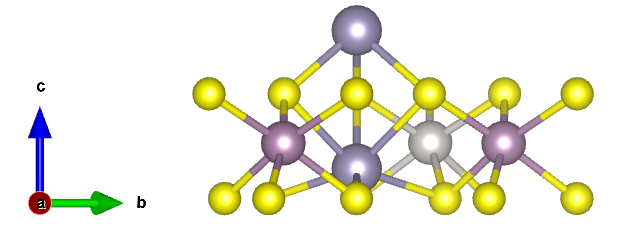
\includegraphics[max width=0.88\linewidth,max height=0.62\textheight,keepaspectratio]{assets/figure-40e35c707e27.png}
\caption{MPSS结构图}
\end{figure}\par


\par\begin{figure}[H]\centering
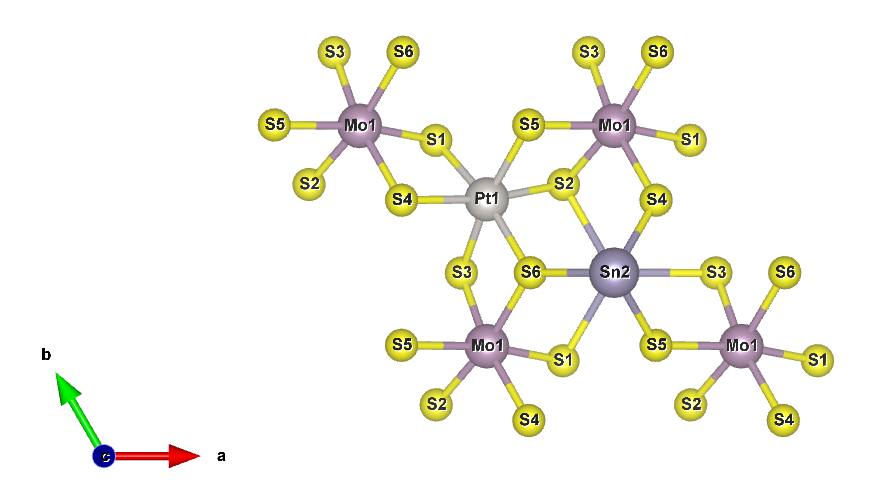
\includegraphics[max width=0.88\linewidth,max height=0.62\textheight,keepaspectratio]{assets/figure-54a09f852c31.png}
\caption{MPSS结构图}
\end{figure}\par


首先准备INCAR\par


\begin{codeindexbox}{代码清单 A.1.1}
语言：python；完整代码见附录第 \pageref{code:1:1} 页，共 38 行。
\end{codeindexbox}


由于是磁性体系,所以要增加很多设置,虽然部分设置是隐式开启或者关闭的,但根据官网的说法,显式地设置出来,也会起到一定的作用。\par


注意,个人习惯先用AGLO=Fast,这样计算速度快,可以快速了解大概的情况,同时第一次计算的时候,可以取小K点,同样使得计算速度快。单层材料不加IVDW范德华修正。 个人习惯开启自旋极化后不设置磁矩,让其自行演化,得到最准确的基态。\par


对于强关联体系,必须加U,具体数值自行测试。\par


准备好POSCAR、POTCAR、CHGCAR、KPOINTS后,提交任务进行计算。\par


\subsection{2. 数据处理方法(重点)}


首先绘制PDOS,这一部分较为繁琐,首先vaspkit/\allowbreak{}114,可以选择原子,输出原子所有轨道的pdos。其它功能进入vaspkit后,自行翻译即可。\par


产生的PDOS\_\allowbreak{}SUM\_\allowbreak{}DW是该原子的数据,复制进orgin表格中。然后把同一轨道的up和down放到一起,再在前面插入x轴——Energy,这一列。全选页面内所有数据后,选择堆积图,调整x和y轴范围即可。\par


成品示例如下:\par


\par\begin{figure}[H]\centering
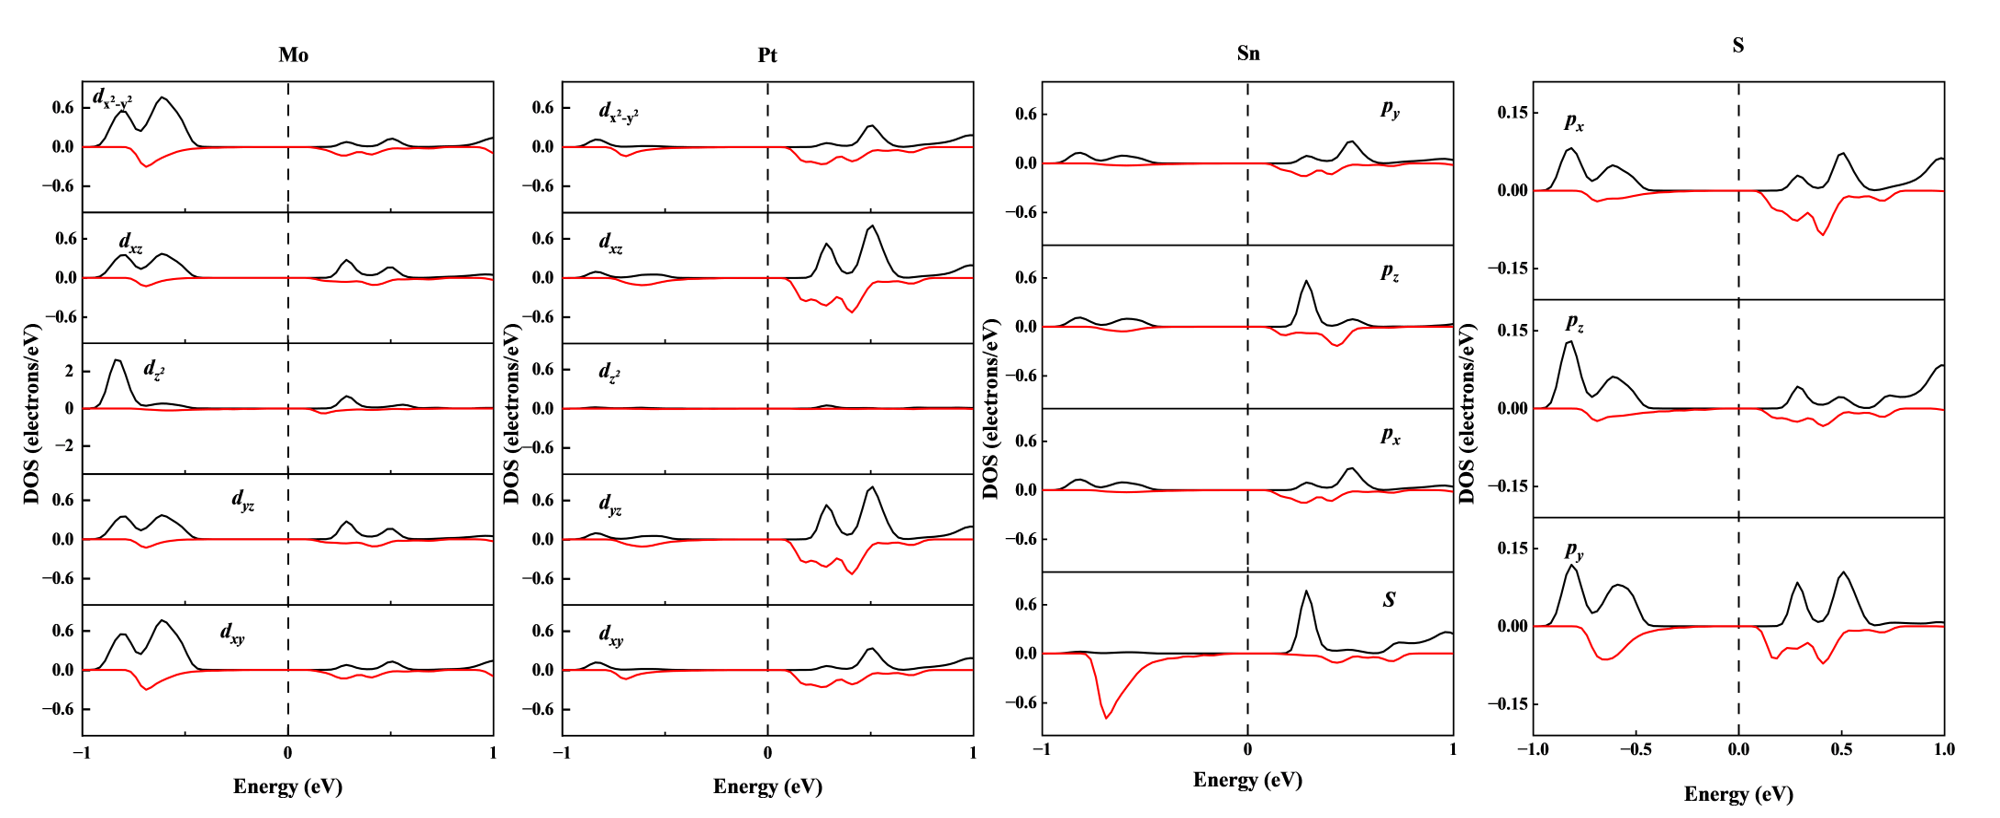
\includegraphics[max width=0.88\linewidth,max height=0.62\textheight,keepaspectratio]{assets/figure-1b796dd54785.png}
\caption{MPSS结构图}
\end{figure}\par


DOS的Origin绘图更为简单,在此不做赘述(同能带计算的数据后处理方式)。\par



\section{vasp计算投影能带}
\begin{articlemeta}
\textbf{日期：}2025-09-24\hfill\textbf{在线原文：}\href{https://marx2001.github.io/sci-note\_posts/20250924-pbands/}{marx2001.github.io}
\end{articlemeta}

\subsubsection{Vasp计算DOS}


投影能带的计算不是必需的,而是在分析机制的时候使用。例如在分析晶体场劈裂情况时需要用到。使用名称为《vasp计算能带》文章中所用的INCAR,计算完成后,输入vaspkit/\allowbreak{}214 即可输出手动选择特定原子的投影能带数据文件。下面是vaspkit投影能带的选取注释:\par


211 标准能带结构(包含所有原子和轨道的投影)\par


212 仅提取单个选定原子的轨道投影能带\par


213 按元素分类(如所有 Fe 原子)的投影能带\par


214 手动选择特定原子(输入原子序号)的投影能带\par


215 按元素权重(如 50\% Fe + 50\% O)的投影能带\par


216 对选定原子和轨道的投影求和(如所有 Fe 的 d 轨道)\par


\textbf{ 1.Origin绘图(重点)}\par


以MPSS为例,其结构如图所示\par


\par\begin{figure}[H]\centering
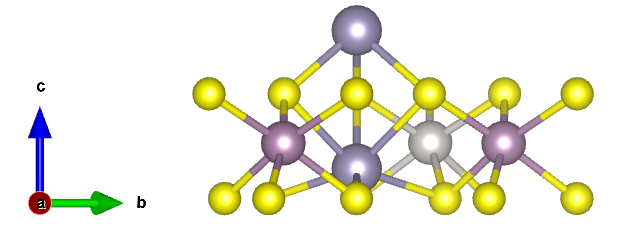
\includegraphics[max width=0.88\linewidth,max height=0.62\textheight,keepaspectratio]{assets/figure-40e35c707e27.png}
\caption{MPSS结构图}
\end{figure}\par


\par\begin{figure}[H]\centering
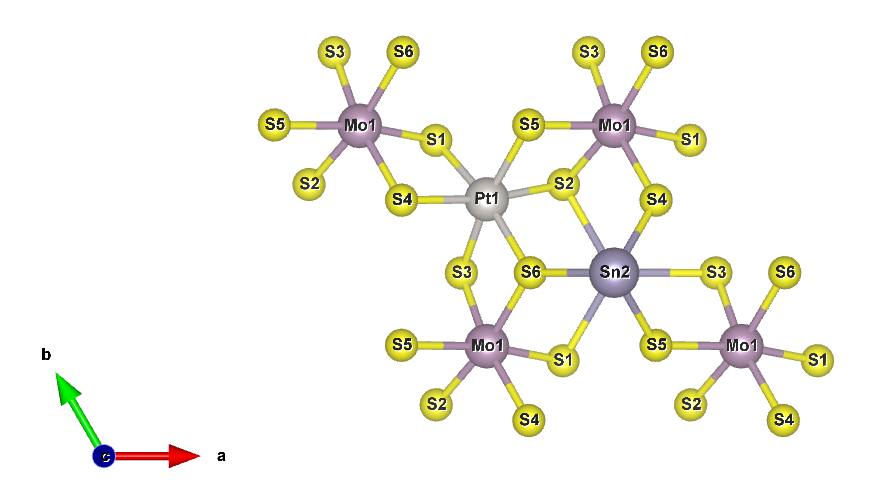
\includegraphics[max width=0.88\linewidth,max height=0.62\textheight,keepaspectratio]{assets/figure-54a09f852c31.png}
\caption{MPSS结构图}
\end{figure}\par


vaspkit/\allowbreak{}214/\allowbreak{}Mo,绘制Mo原子的投影能带\par


\par\begin{figure}[H]\centering
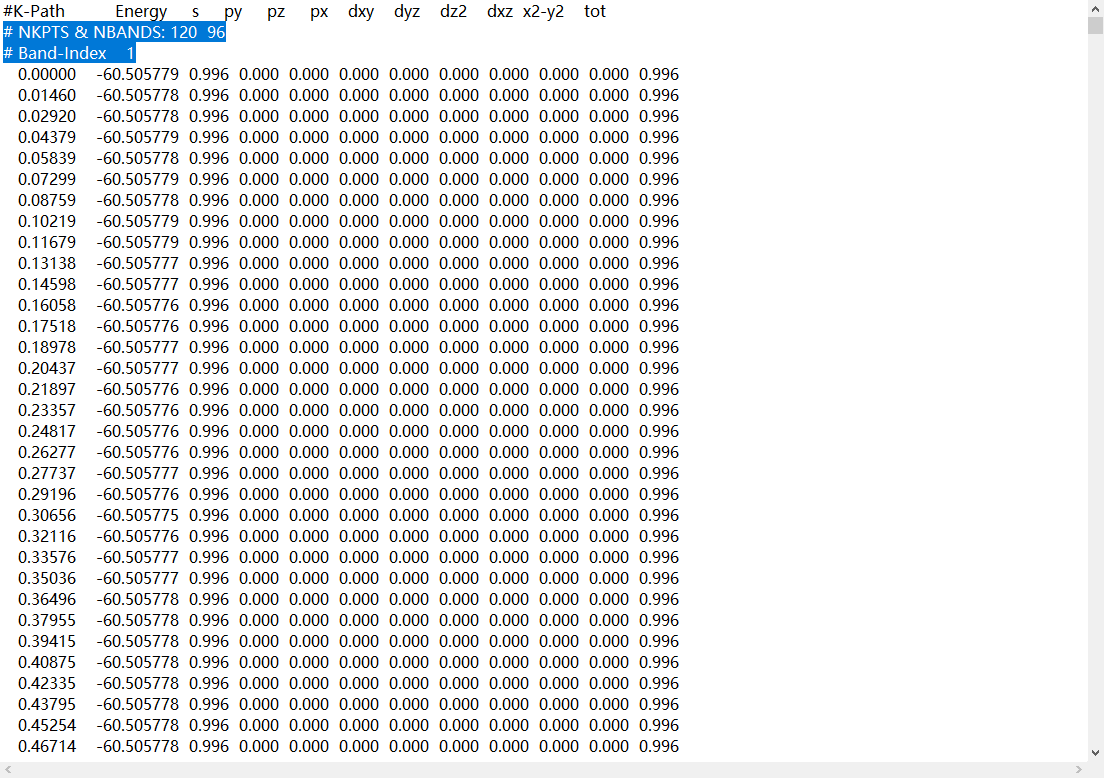
\includegraphics[max width=0.88\linewidth,max height=0.62\textheight,keepaspectratio]{assets/figure-5a34edce6c50.png}
\caption{第一步}
\end{figure}\par


如上图所示,得到数据文件PBAND\_\allowbreak{}SUM\_\allowbreak{}DW.dat和PBAND\_\allowbreak{}SUM\_\allowbreak{}UP.dat文件。删除上图中选中的两行,便于在origin中直接作为标签。\par


如下图所示,直接将数据文件拖到origin中:\par


\par\begin{figure}[H]\centering
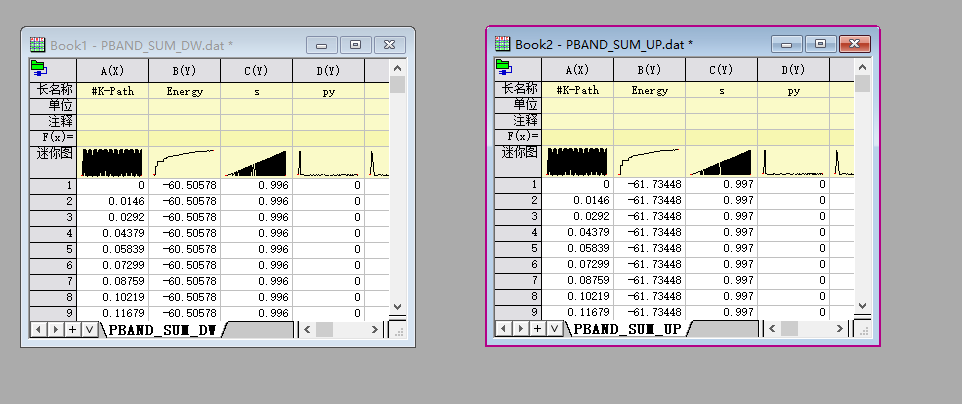
\includegraphics[max width=0.88\linewidth,max height=0.62\textheight,keepaspectratio]{assets/figure-e8881ea13984.png}
\caption{第一步}
\end{figure}\par


选中如图所示两行画图,如下图所示\par


\par\begin{figure}[H]\centering
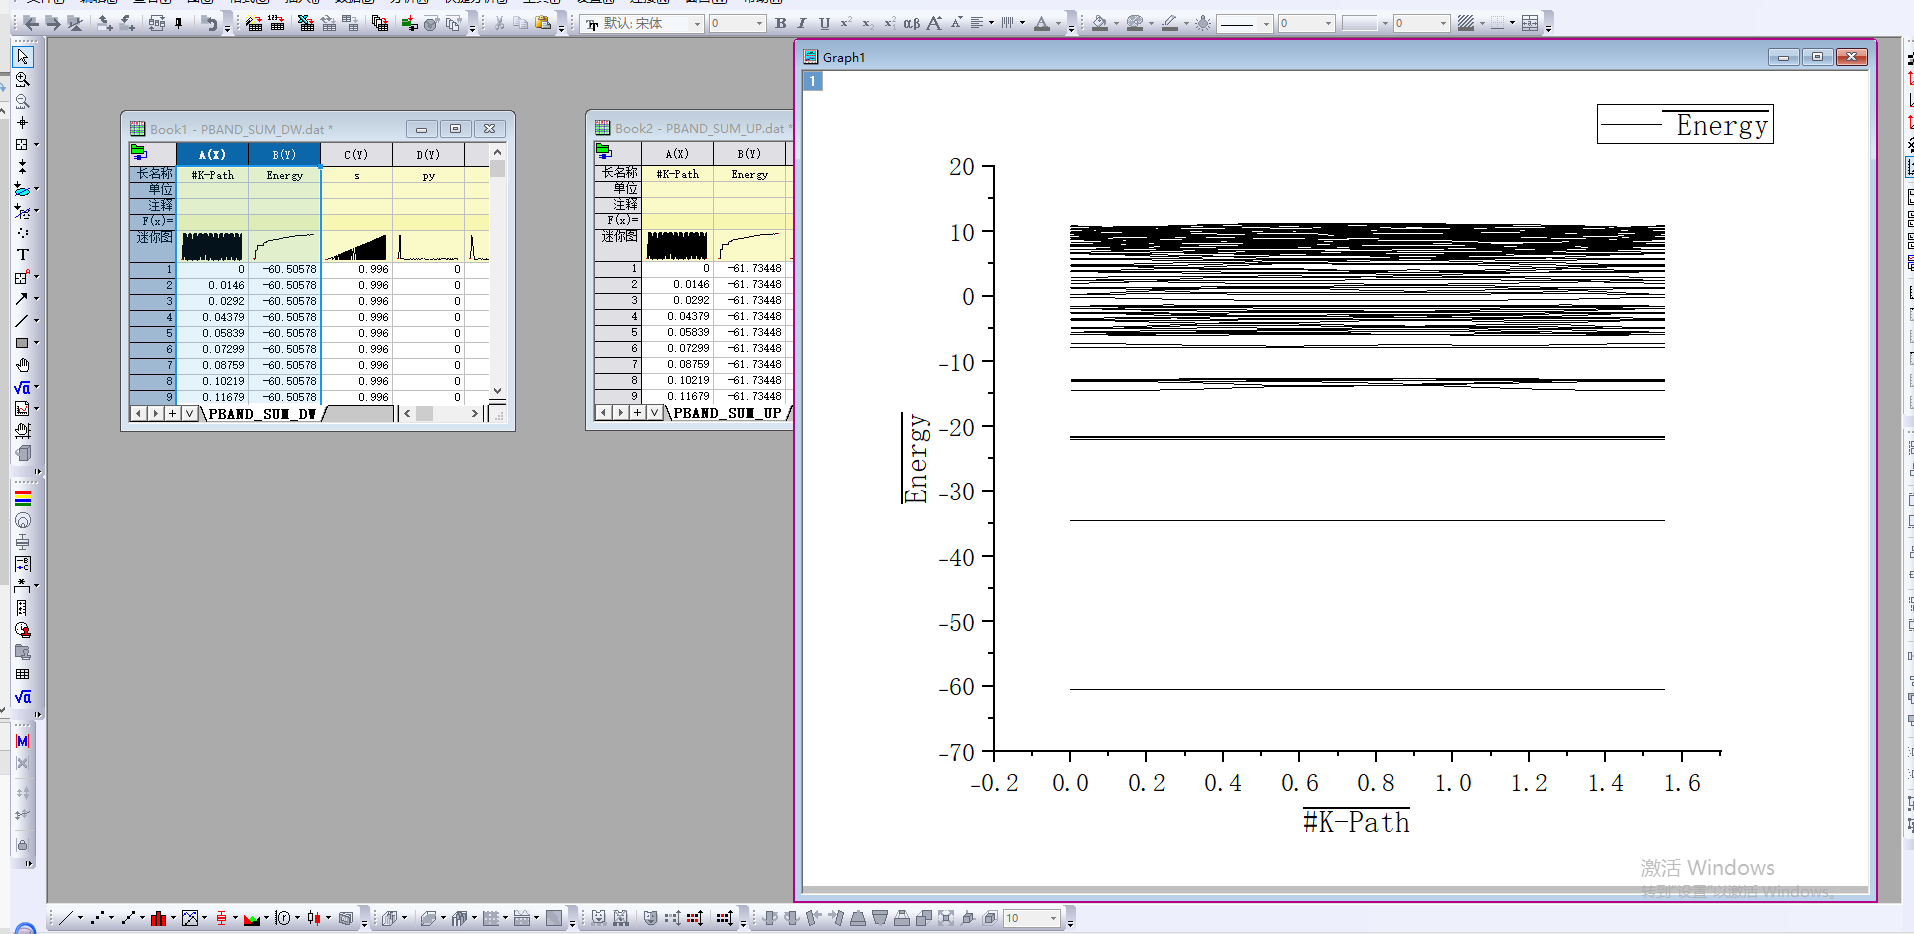
\includegraphics[max width=0.88\linewidth,max height=0.62\textheight,keepaspectratio]{assets/figure-1f4912869950.png}
\caption{b3}
\end{figure}\par


双击1,进入图层,选中十个新添加的图层,点击2成组,点击3,修改成散点图\par


\par\begin{figure}[H]\centering
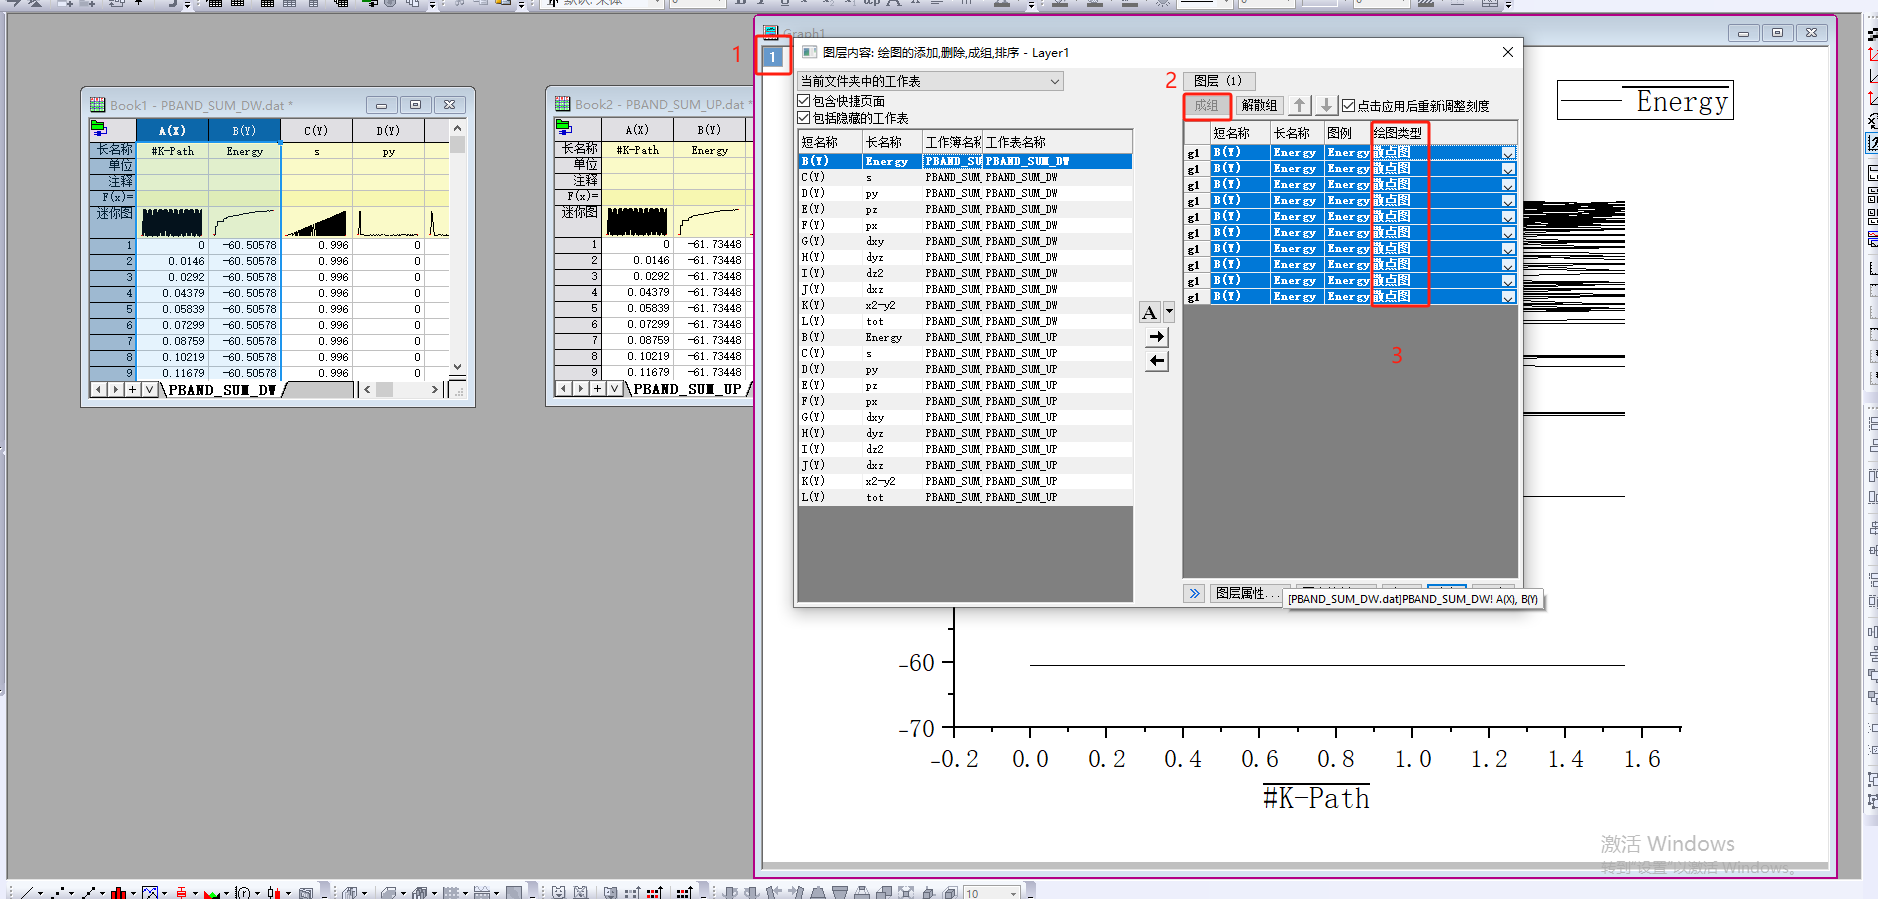
\includegraphics[max width=0.88\linewidth,max height=0.62\textheight,keepaspectratio]{assets/figure-7e1c9a53ab05.png}
\caption{b3}
\end{figure}\par


双击图像(红框区域),弹出来对话框\par


\par\begin{figure}[H]\centering
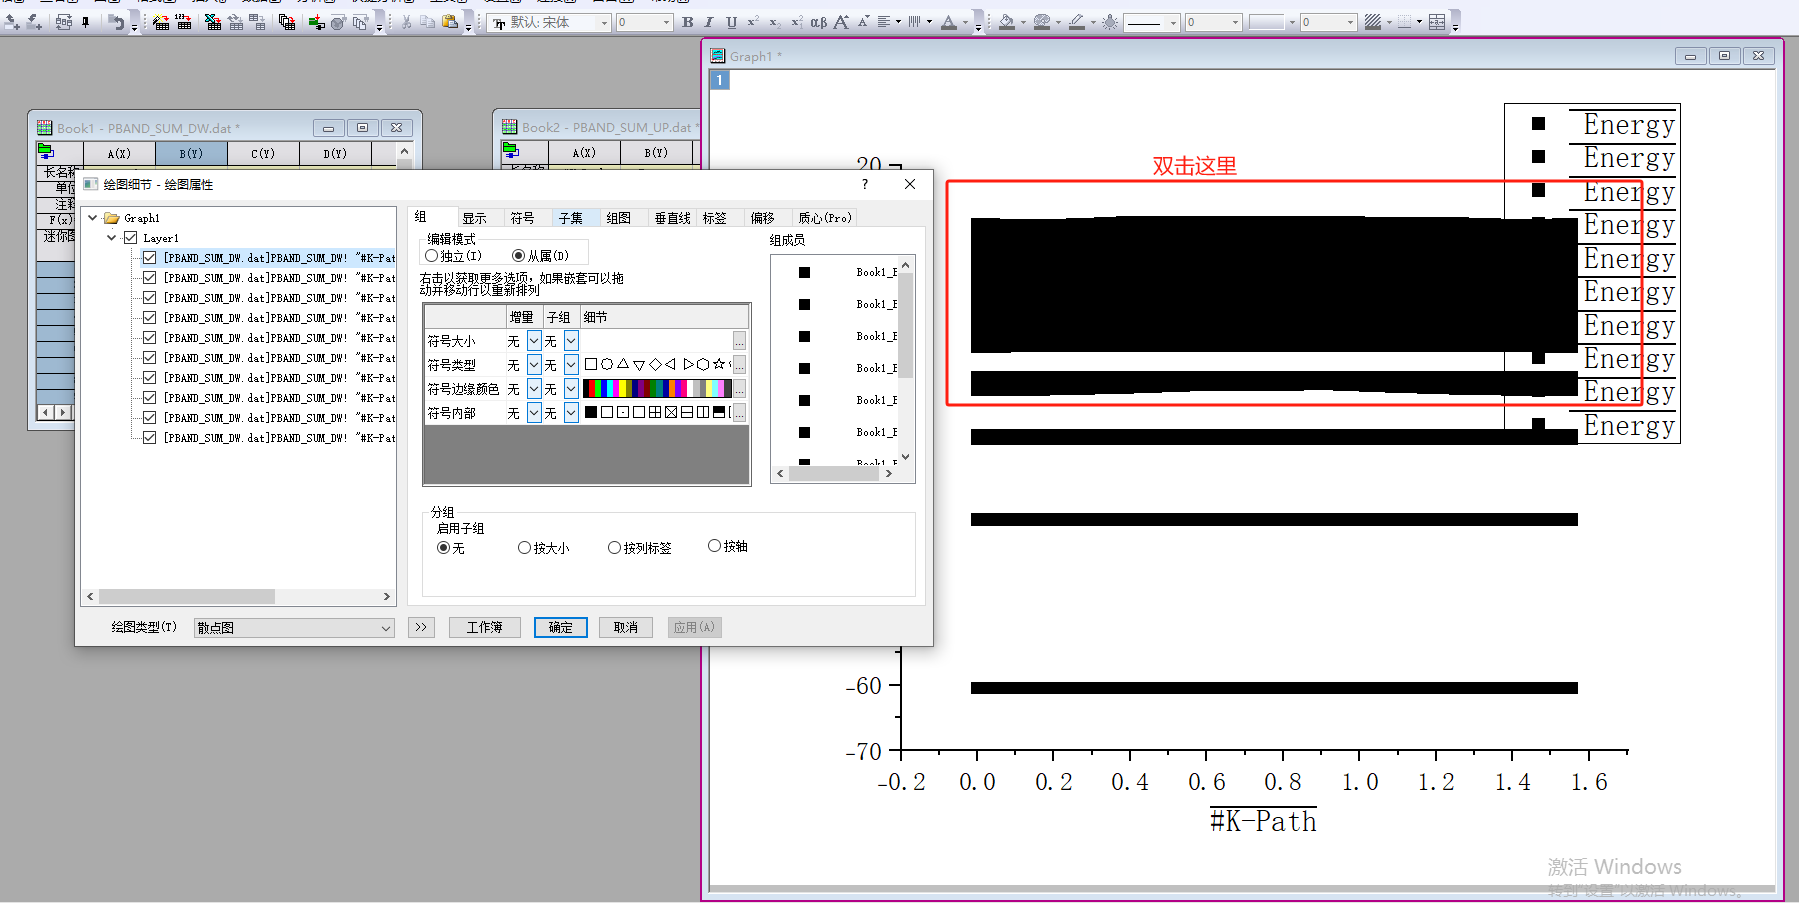
\includegraphics[max width=0.88\linewidth,max height=0.62\textheight,keepaspectratio]{assets/figure-dec9c76efb7e.png}
\caption{b3}
\end{figure}\par


修改如下图所示的三个参数,缩放因子建议20。\par


\par\begin{figure}[H]\centering
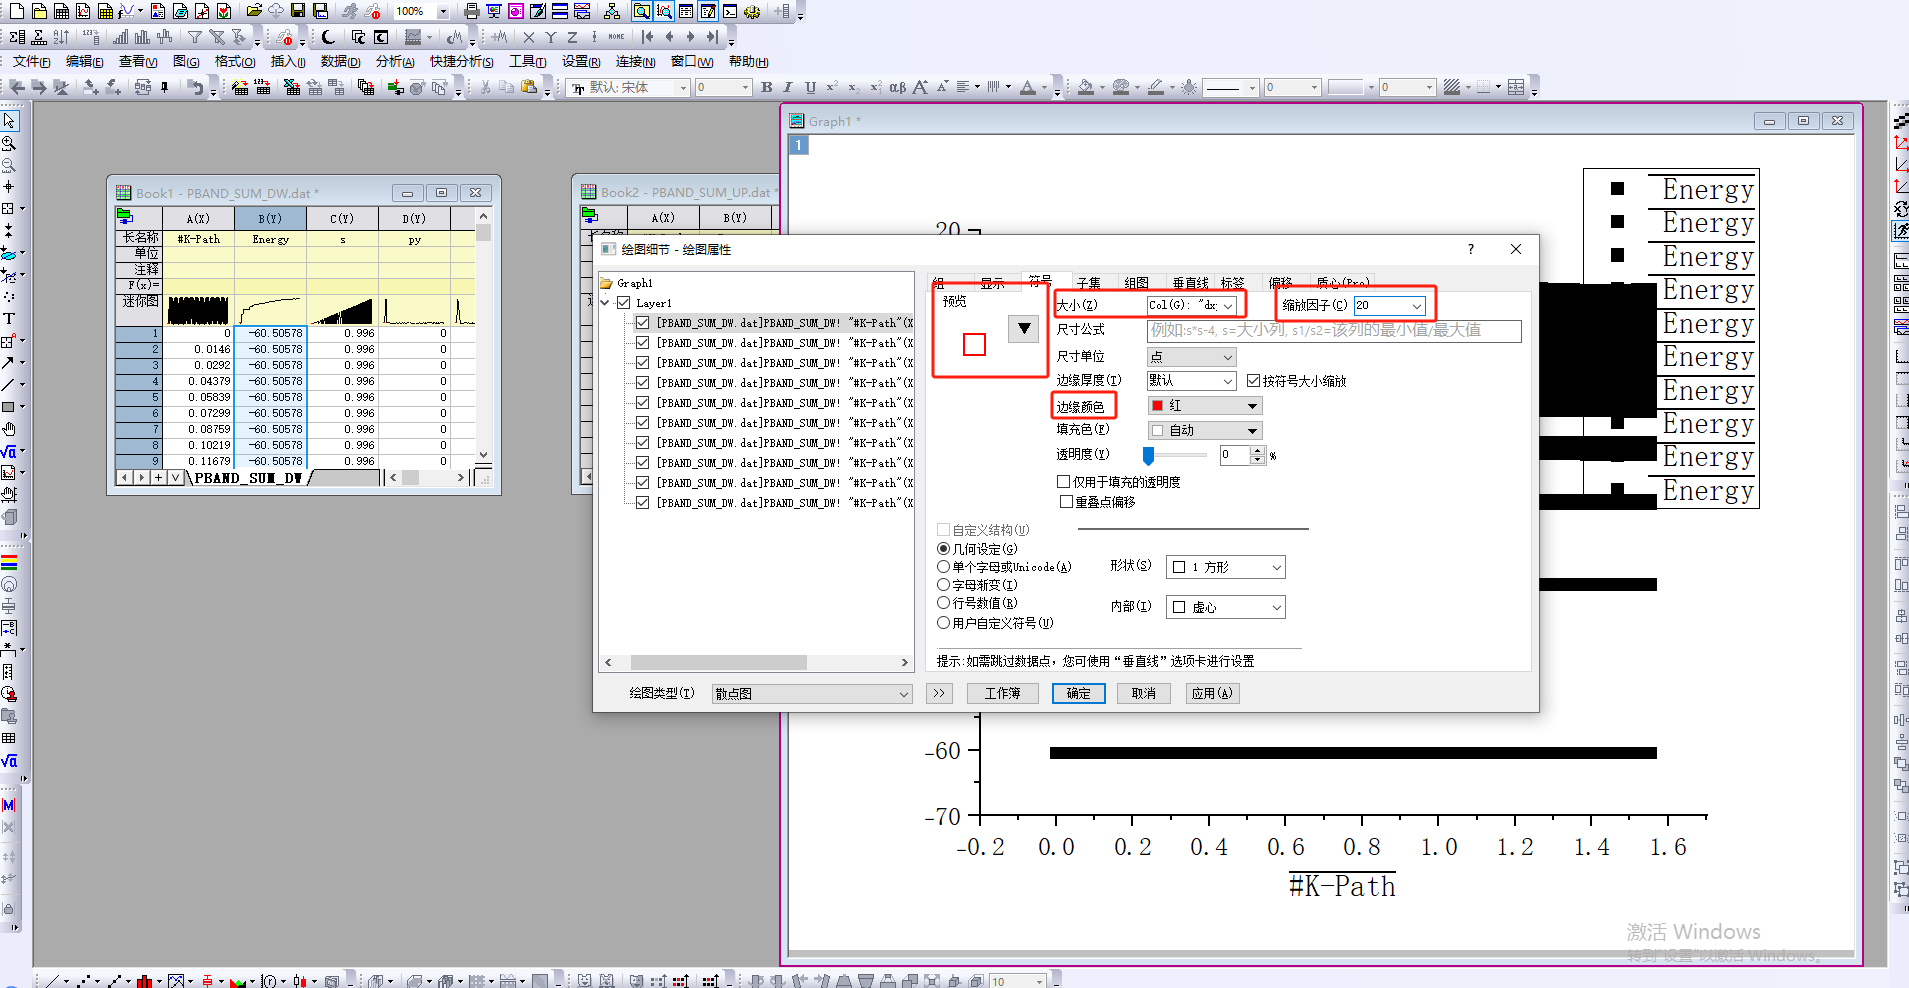
\includegraphics[max width=0.88\linewidth,max height=0.62\textheight,keepaspectratio]{assets/figure-c5630de09945.png}
\caption{b3}
\end{figure}\par


注意事项——反铁磁基态,可以任意选择能量折线图,而铁磁基态,由于能带spin up和spin down不简并,所以绘图时要注意,Energy折线图up要选5个(d轨道,p轨道选3个),down要选五个。\par


原因是投影能带是算的每个轨道相比于Energy的权重,而反铁磁基态的能量是简并的,所以选up和down的均可,不影响权重计算,而铁磁基态由于作为分母的总能量不简并,所以若想准确计算权重,能量折线图(分母)必须一半up一半down。\par


最终效果图:\par


\par\begin{figure}[H]\centering
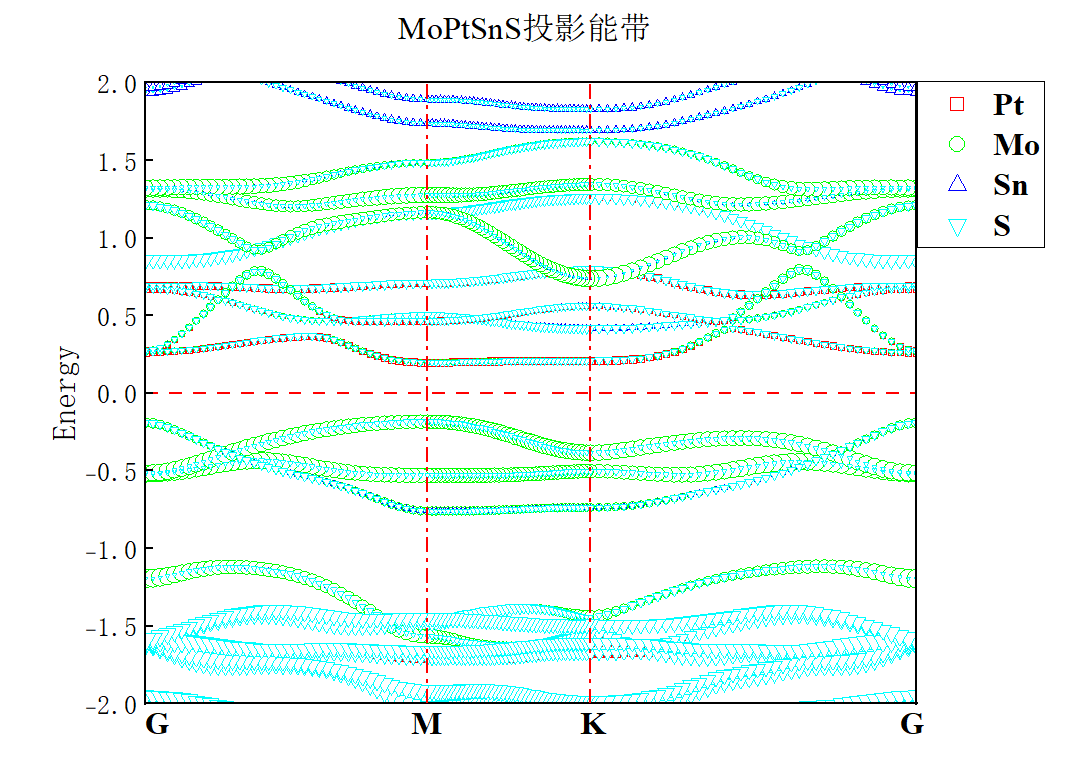
\includegraphics[max width=0.88\linewidth,max height=0.62\textheight,keepaspectratio]{assets/figure-266885fad17b.png}
\caption{b3}
\end{figure}\par


\textbf{ 2.自定义脚本绘图(原创)}\par


该脚本功能较为完善,支持灵活自定义参数,使用方式类似 VASPKIT。首先需要采用如下目录结构:\par


\begin{codeindexbox}{代码清单 A.2.1}
语言：python；完整代码见附录第 \pageref{code:2:1} 页，共 19 行。
\end{codeindexbox}


自旋极化的投影能带绘制,代码如下:\par


\begin{codeindexbox}{代码清单 A.2.2}
语言：python；完整代码见附录第 \pageref{code:2:2} 页，共 658 行。
\end{codeindexbox}


Usage\par


\begin{codeindexbox}{代码清单 A.2.3}
语言：python；完整代码见附录第 \pageref{code:2:3} 页，共 70 行。
\end{codeindexbox}


考虑SOC非自旋极化的情况下的代码:\par


\begin{codeindexbox}{代码清单 A.2.4}
语言：python；完整代码见附录第 \pageref{code:2:4} 页，共 651 行。
\end{codeindexbox}


运行命令绘制Ge的p轨道分布\par


\begin{inlinecodebox}{短代码 · python}
\VerbatimInput[fontsize=\small,breaklines=true,breakanywhere=true,tabsize=2,listparameters={\setlength{\topsep}{0pt}\setlength{\partopsep}{0pt}\setlength{\parsep}{0pt}}]{code/002-005.py}
\end{inlinecodebox}



\section{vasp计算能带}
\begin{articlemeta}
\textbf{日期：}2025-09-24\hfill\textbf{在线原文：}\href{https://marx2001.github.io/sci-note\_posts/20250924-band/}{marx2001.github.io}
\end{articlemeta}

能带计算作为最基本的计算,也有其合理的步骤以及注意事项。\par


\textbf{ 1. 静态自洽计算(static)}\par


以MPSS为例,其结构如图所示\par


\par\begin{figure}[H]\centering
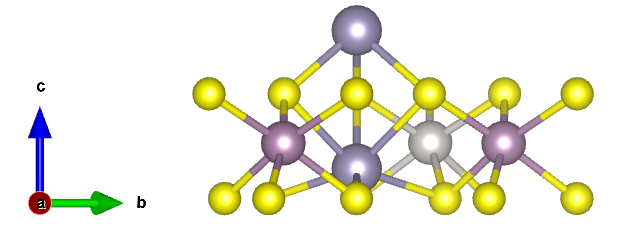
\includegraphics[max width=0.88\linewidth,max height=0.62\textheight,keepaspectratio]{assets/figure-40e35c707e27.png}
\caption{MPSS结构图}
\end{figure}\par


\par\begin{figure}[H]\centering
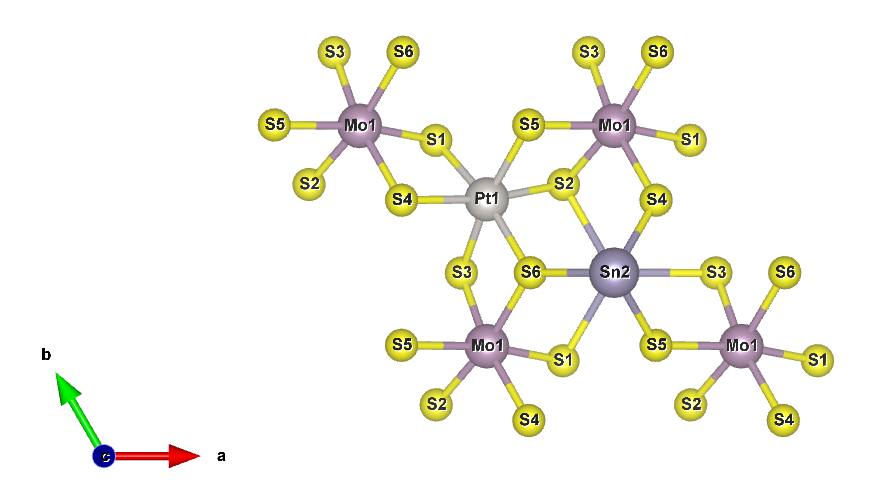
\includegraphics[max width=0.88\linewidth,max height=0.62\textheight,keepaspectratio]{assets/figure-54a09f852c31.png}
\caption{MPSS结构图}
\end{figure}\par


首先准备INCAR\par


\begin{codeindexbox}{代码清单 A.3.1}
语言：python；完整代码见附录第 \pageref{code:3:1} 页，共 36 行。
\end{codeindexbox}


由于是磁性体系,所以要增加很多设置,虽然部分设置是隐式开启或者关闭的,但根据官网的说法,显式地设置出来,也会起到一定的作用。\par


注意,个人习惯先用AGLO=Fast,这样计算速度快,可以快速了解大概的情况,同时第一次计算的时候,可以取小K点,同样使得计算速度快。单层材料不加IVDW范德华修正。 个人习惯开启自旋极化后不设置磁矩,让其自行演化,得到最准确的基态。static计算较快,因此不设置混合系数也是可以的。\par


LCHARG必须开启,因为能带计算必须要用到CHGCAR才能足够精确。\par


对于强关联体系,必须加U,具体数值自行测试。\par


提交static任务计算脚本后等待结果。\par


\subsection{2. 进行能带计算(重点)}


这个计算需要注意一个情况,必须设置ISTART=1,ICHARG=11,原因如下方注释所言。而且NBANDS不要设置,避免浪费时间。band计算不开启自旋轨道耦合(SOC),如果想看考虑自旋轨道耦合的结果,则取消LSORBIT和LORBMOM的注释即可。\par


INCAR如下\par


\begin{codeindexbox}{代码清单 A.3.2}
语言：python；完整代码见附录第 \pageref{code:3:2} 页，共 37 行。
\end{codeindexbox}


KPOINTS用vaspkit/\allowbreak{}302,生成,不要用static的KPOINTS,同时也可以前往SeekKPATH网站自定义高对称点路径。\par


准备好INCAR、CHGCAR、POSCAR、POTCAR后提交计算即可。\par


\subsection{3. 数据处理}


计算结束后,vaspkit/\allowbreak{}211,产生BAND.dat和KLINES.dat文件,打开文件后,复制内容到Origin当中,先复制BAND.dat数据,再在band数据后添加列,复制进KLINTS.dat数据,并右键选中列后设置为X轴。再点击左下角绘图,点击右上角让曲线更平滑,然后选择数据范围,一般只看费米能级附近的能带,所以y轴范围[-2,2].其它格式自行调节。\par



\section{vasp计算磁耦合参数大小}
\begin{articlemeta}
\textbf{日期：}2025-09-25\hfill\textbf{在线原文：}\href{https://marx2001.github.io/sci-note\_posts/20250925-J}{marx2001.github.io}
\end{articlemeta}

为了研究二维材料的拓扑自旋纹理,我们需要计算海森堡模型中的DMI的能量大小。\par


磁耦合参数,即磁性原子之间相互作用的大小。J>0,磁矩倾向于平行排列,即铁磁(FM);J<0,磁矩倾向于反平行排列,即反铁磁(AFM)。J的大小决定磁耦合的强弱。J大,相互作用强,居里温度/\allowbreak{}尼尔温度高。J小,相互作用弱,热涨落容易破坏有序性。\par


J源于电子的交换效应和电子-电子相互作用,包括直接交换、超交换、超超交换、双交换以及RKKY相互作用。\par


J决定自旋是FM还是AFM,DMI倾向于让自旋扭转,形成螺旋或者畴壁。\par


\textbf{ 1. 能量法计算J值}\par


以MPSS为例,其结构如图所示\par


\par\begin{figure}[H]\centering
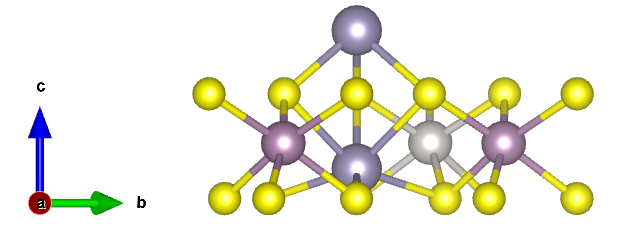
\includegraphics[max width=0.88\linewidth,max height=0.62\textheight,keepaspectratio]{assets/figure-40e35c707e27.png}
\caption{MPSS结构图}
\end{figure}\par


\par\begin{figure}[H]\centering
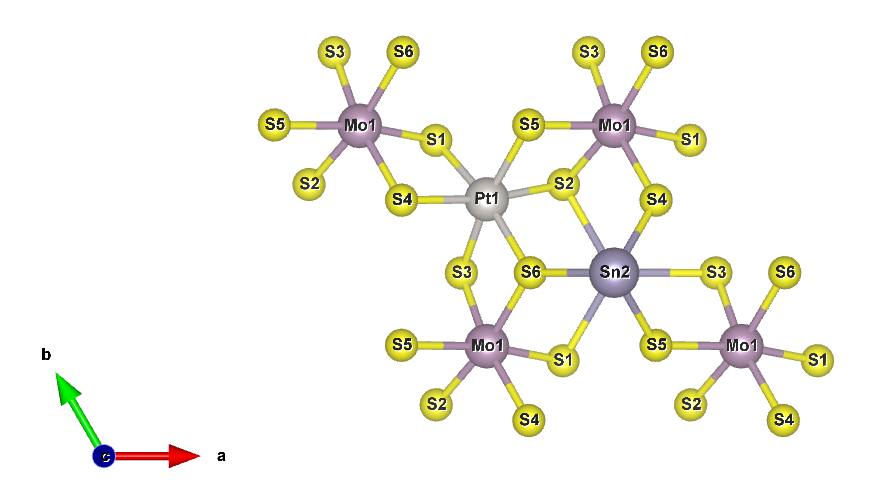
\includegraphics[max width=0.88\linewidth,max height=0.62\textheight,keepaspectratio]{assets/figure-54a09f852c31.png}
\caption{MPSS结构图}
\end{figure}\par


需要准备四个INCAR,四个INCAR的唯一区别就是磁态设置——FM、Neel、Stripy、Zigzag。如下图所示,箭头为磁矩方向:\par

 
\par\begin{figure}[H]\centering
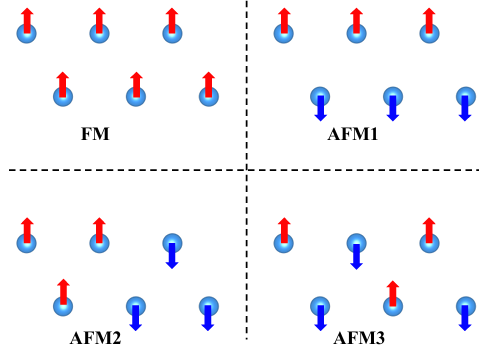
\includegraphics[max width=0.88\linewidth,max height=0.62\textheight,keepaspectratio]{assets/figure-7101d4c54cf9.png}
\caption{Fig1}
\end{figure}\par
 

四种INCAR如下方所示\par


INCAR1:\par


\begin{codeindexbox}{代码清单 A.4.1}
语言：shell；完整代码见附录第 \pageref{code:4:1} 页，共 40 行。
\end{codeindexbox}


INCAR2\par


\begin{codeindexbox}{代码清单 A.4.2}
语言：shell；完整代码见附录第 \pageref{code:4:2} 页，共 40 行。
\end{codeindexbox}


INCAR3\par


\begin{codeindexbox}{代码清单 A.4.3}
语言：shell；完整代码见附录第 \pageref{code:4:3} 页，共 40 行。
\end{codeindexbox}


INCAR4\par


\begin{codeindexbox}{代码清单 A.4.4}
语言：shell；完整代码见附录第 \pageref{code:4:4} 页，共 40 行。
\end{codeindexbox}


由于是磁性体系,所以要增加很多设置,虽然部分设置是隐式开启或者关闭的,但根据官网的说法,显式地设置出来,也会起到一定的作用。\par


注意,个人习惯先用AGLO=Fast,这样计算速度快,可以快速了解大概的情况,同时第一次计算的时候,可以取小K点,同样使得计算速度快。单层材料不加IVDW范德华修正。 个人习惯开启自旋极化后不设置磁矩,让其自行演化,得到最准确的基态。\par


对于强关联体系,必须加U,具体数值自行测试。\par


由于要设置四种磁态,所以要进行扩胞,根据三近邻海森堡模型,MPSS的扩胞大小要包含任意磁性原子的第三近邻磁性原子。显而易见,对于MPSS材料体系,需要扩胞3\emph{3}1。\par


准备好POSCAR、POTCAR、KPOINTS后,提交任务进行计算。任务脚本如下:\par


\begin{codeindexbox}{代码清单 A.4.5}
语言：shell；完整代码见附录第 \pageref{code:4:5} 页，共 41 行。
\end{codeindexbox}


计算完成后,键入qvasp -e,得到四个能量,进入这个网址:http:/\allowbreak{}/\allowbreak{}www.yunsuan.info/\allowbreak{}matrixcomputations/\allowbreak{}solvelinearsystems.html,解线性方程组,其系数如下所示:\par

 
\par\begin{figure}[H]\centering
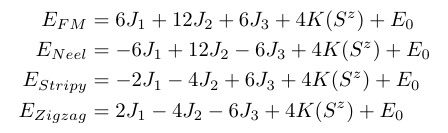
\includegraphics[max width=0.88\linewidth,max height=0.62\textheight,keepaspectratio]{assets/figure-7cf18de24b7d.png}
\caption{Fig1}
\end{figure}\par
 

\textbf{ 2. 四态法计算J值}\par


计算量非常大,不推荐此种方法。四态法最好使用ncl计算,较为准确。另外,如果算z方向,则是把磁矩设置到z方向上,如果计算y方向,就把磁矩设置到y方向上。\par


方法原理同四态法计算DMI,因此直接放上4个INCAR文件和提交任务脚本:\par


INCAR1\par


\begin{codeindexbox}{代码清单 A.4.6}
语言：shell；完整代码见附录第 \pageref{code:4:6} 页，共 46 行。
\end{codeindexbox}


INCAR2\par


\begin{codeindexbox}{代码清单 A.4.7}
语言：shell；完整代码见附录第 \pageref{code:4:7} 页，共 41 行。
\end{codeindexbox}


INCAR3\par


\begin{codeindexbox}{代码清单 A.4.8}
语言：shell；完整代码见附录第 \pageref{code:4:8} 页，共 41 行。
\end{codeindexbox}


INCAR4\par


\begin{codeindexbox}{代码清单 A.4.9}
语言：shell；完整代码见附录第 \pageref{code:4:9} 页，共 41 行。
\end{codeindexbox}


提交任务脚本为:\par


\begin{codeindexbox}{代码清单 A.4.10}
语言：shell；完整代码见附录第 \pageref{code:4:10} 页，共 51 行。
\end{codeindexbox}


\chapter{磁性参数与 DMI}
\begin{partbox}本专题收录 2 篇文章。\end{partbox}

\section{vasp计算DMI大小}
\begin{articlemeta}
\textbf{日期：}2025-09-25\hfill\textbf{在线原文：}\href{https://marx2001.github.io/sci-note\_posts/20250925-D}{marx2001.github.io}
\end{articlemeta}

为了研究二维材料的拓扑自旋纹理,我们需要计算海森堡模型中的DMI的能量大小。\par


DMI的大小取决于两个核心条件——对称性和自旋轨道耦合。只有存在较强的自旋轨道耦合(SOC),才有可能产生DMI。这是因为DMI本质上来源于SOC对超交换相互作用的修正。\par


在轻元素体系里,SOC很弱,DMI可以忽略。\par


含有重元素(如过渡金属、5d元素、Bi,W,Ir等)或者与重原子基地相耦合的二维材料,更容易产生显著的DMI。\par


根据Moriya定理,缺乏空间反演对称性,如果两个磁性原子之间的中点存在反演中心,对应的DMI为0.因此在二位材料中产生DMI,需要在结构上产生破缺的对称性。\par


例如:固有结构的不对称、缺陷或表面不对称;界面或基底效应;外场诱导(电场或者应变导致结构对称性破缺)\par


点群限制:DMI的方向由晶体对称性决定。二维材料中,常见的 C3v、C2v 等对称性都可能允许 DM 相互作用。\par


\textbf{ 1. 能量法的计算步骤}\par


以MPSS为例,其结构如图所示\par


\par\begin{figure}[H]\centering
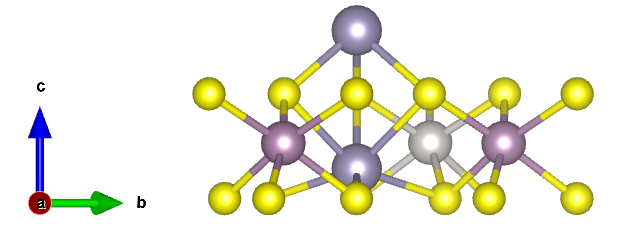
\includegraphics[max width=0.88\linewidth,max height=0.62\textheight,keepaspectratio]{assets/figure-40e35c707e27.png}
\caption{MPSS结构图}
\end{figure}\par


\par\begin{figure}[H]\centering
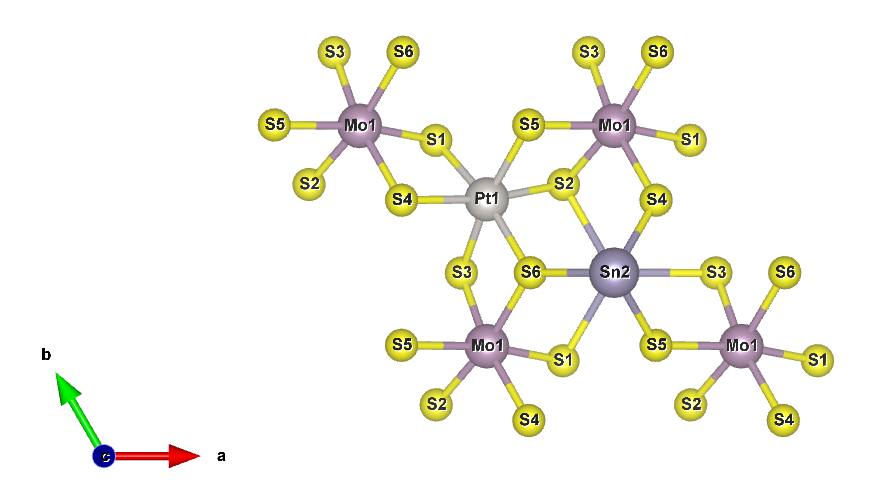
\includegraphics[max width=0.88\linewidth,max height=0.62\textheight,keepaspectratio]{assets/figure-54a09f852c31.png}
\caption{MPSS结构图}
\end{figure}\par


首先准备INCAR\par


\begin{codeindexbox}{代码清单 A.5.1}
语言：python；完整代码见附录第 \pageref{code:5:1} 页，共 39 行。
\end{codeindexbox}


需要注意的是,能量法的原理是设置磁态为顺时针的能量减去逆时针的能量再除以一个系数,所以我们需要在ISPIN=2的情况下,设置磁矩为顺时针的方向。\par


由于是磁性体系,所以要增加很多设置,虽然部分设置是隐式开启或者关闭的,但根据官网的说法,显式地设置出来,也会起到一定的作用。\par


注意,个人习惯先用AGLO=Fast,这样计算速度快,可以快速了解大概的情况,同时第一次计算的时候,可以取小K点,同样使得计算速度快。单层材料不加IVDW范德华修正。 个人习惯开启自旋极化后不设置磁矩,让其自行演化,得到最准确的基态。\par


对于强关联体系,必须加U,具体数值自行测试。\par


由于要设置顺时针四个方向的磁矩,只有一个磁性原子显然是不够的,所以我们需要在x方向扩4倍于原胞大小的超胞,在shell面板内,输入vaspkt/\allowbreak{}401/\allowbreak{}4 1 1,注意411之间要加空格。\par


得到SUPERCELL411.vasp文件后,修改名称为POSCAR。\par


接下来准备KPOINTS,有一个细节,不要使用之前计算的KPOINTS,而是要再次键入vaspkit/\allowbreak{}102/\allowbreak{}1/\allowbreak{}102/\allowbreak{}0.03,得到KPOINTS。\par


准备好POSCAR、POTCAR、KPOINTS后,提交任务进行计算。任务脚本如下:\par


\begin{codeindexbox}{代码清单 A.5.2}
语言：shell；完整代码见附录第 \pageref{code:5:2} 页，共 39 行。
\end{codeindexbox}


等待计算结束后,键入qvasp -e,收集能量信息,cw的能量减去acw的能量除以一个系数即可。这个系数根据体系而定,可以参考具体的文献。\par


\textbf{ 1. 四态法的计算步骤}\par


四态法是指通过构建四种磁态,通过求解这四个海森堡模型哈密顿方程的方程组来得到对应的磁耦合参数,具有一般性,但计算量相比于能量法较大,对于原胞内原子数目较多的大体系而言,设备要求较高。\par


应用四态法计算DMI,首先要构建超胞,以MPSS的三角晶格为例,由于两个磁性原子之间的距离为0.637nm,所以我们选择扩3\emph{3}1的超胞,使得相邻周期同一原子的距离大于0.15nm,以屏蔽相邻周期同一磁性原子的影响。\par


然后构建四个磁态,这四个磁态分别是均是朝上的铁磁,一上一下反铁磁+其它磁性原子向上、一下以上+其他磁性原子向上、同下+其他磁性原子向上。运行计算任务后,E1+E4-E2-E3的结果再除以4即可,为了得到真实的能量,需要再除以自旋的平方,自旋量子数的数值是原胞磁矩的值除以2.\par


提交计算任务的脚本为:\par


\begin{codeindexbox}{代码清单 A.5.3}
语言：shell；完整代码见附录第 \pageref{code:5:3} 页，共 46 行。
\end{codeindexbox}



\section{(文献整理)块体材料 DMI 的第一性原理提取方法}
\begin{articlemeta}
\textbf{日期：}2026-07-08\hfill\textbf{在线原文：}\href{https://marx2001.github.io/sci-note\_posts/20260708DMI}{marx2001.github.io}
\end{articlemeta}

\subsubsection{说明}


本文整理用于\textbf{块体材料 Dzyaloshinskii–Moriya interaction(DMI)第一性原理计算与提取}的代表性文献。重点不是介绍 DMI 的物理起源,而是给后续实际计算提供文献依据,包括:\par


\begin{codeindexbox}{代码清单 A.6.1}
语言：shell；完整代码见附录第 \pageref{code:6:1} 页，共 5 行。
\end{codeindexbox}


对于块体材料,DMI 一般不应只写成一个标量 (D),而应写成每一类磁性键的 DMI 矢量:\par


[ H\_\allowbreak{}\textbackslash{}\allowbreak{}mathrm\{DMI\} = \textbackslash{}\allowbreak{}sum\_\allowbreak{}\{ij\}\textbackslash{}\allowbreak{}mathbf\{D\}\_\allowbreak{}\{ij\}\textbackslash{}\allowbreak{}cdot \textbackslash{}\allowbreak{}left(\textbackslash{}\allowbreak{}mathbf\{e\}\_\allowbreak{}i\textbackslash{}\allowbreak{}times\textbackslash{}\allowbreak{}mathbf\{e\}\_\allowbreak{}j\textbackslash{}\allowbreak{}right) ]\par


或者根据文献约定写成带负号的形式:\par


[ H\_\allowbreak{}\textbackslash{}\allowbreak{}mathrm\{DMI\} = -\textbackslash{}\allowbreak{}sum\_\allowbreak{}\{ij\}\textbackslash{}\allowbreak{}mathbf\{D\}\_\allowbreak{}\{ij\}\textbackslash{}\allowbreak{}cdot \textbackslash{}\allowbreak{}left(\textbackslash{}\allowbreak{}mathbf\{e\}\_\allowbreak{}i\textbackslash{}\allowbreak{}times\textbackslash{}\allowbreak{}mathbf\{e\}\_\allowbreak{}j\textbackslash{}\allowbreak{}right) ]\par


因此,在引用文献或写计算方法时,必须明确自己的哈密顿量符号约定。\par


\medskip\hrule\medskip


\subsubsection{文献总览}


\begin{center}\small
\begin{longtable}{@{}p{0.200\textwidth} p{0.200\textwidth} p{0.200\textwidth} p{0.200\textwidth}@{}}
\toprule
序号 & 文献 & 方法类型 & 适合用途 \\
\midrule
1 & Yang, Liang \& Cui, Nat. Rev. Phys. 2023 & DMI 第一性原理综述 & 总述引用 \\
2 & Xiang et al., Dalton Trans. 2013 & 能量映射综述 & 说明 spin Hamiltonian /\allowbreak{} energy mapping \\
3 & Šabani et al., Phys. Rev. B 2020 & 通用四态映射 & 提取完整 exchange matrix \\
4 & Xu et al., Phys. Rev. B 2019 & BiFeO3 四态映射 & 块体多铁材料 DMI 案例 \\
5 & Xu et al., Phys. Rev. B 2021 & BiFeO3 spin spiral & 用 (E(q)) 提取 DMI \\
6 & Yang et al., Phys. Rev. Lett. 2012 & Cu2OSeO3 DMI & 块体手性磁体 /\allowbreak{} 多铁材料案例 \\
7 & Loh \& Gan, AIP Adv. 2017 & bulk FeGe spin spiral /\allowbreak{} SOC & 块体 B20 手性磁体案例 \\
8 & Koretsune et al., Sci. Rep. 2015 & Wannier /\allowbreak{} first-principles DMI & Mn1-xFexGe 中 DMI 大小和符号调控 \\
9 & He et al., Comput. Phys. Commun. 2021 & TB2J /\allowbreak{} Green’s function & 自动提取 (J\_\allowbreak{}\{ij\})、(\textbackslash{}\allowbreak{}mathbf\{D\}\_\allowbreak{}\{ij\}) \\
10 & Mahfouzi \& Kioussis, Phys. Rev. B 2021 & Green’s function DMI & Green’s function 方法依据 \\
\bottomrule
\end{longtable}
\end{center}


\medskip\hrule\medskip


\subsubsection{方法分类}


\subsubsection{1. 四态能量映射法}


四态能量映射法适合从总能差中提取某一对磁性原子的交换矩阵。对于两个自旋 (i,j),一般写成:\par


[ H\_\allowbreak{}\{ij\} = \textbackslash{}\allowbreak{}mathbf\{S\}\emph{i \textbackslash{}\allowbreak{}mathbf\{J\}}\{ij\} \textbackslash{}\allowbreak{}mathbf\{S\}\_\allowbreak{}j ]\par


其中 (\textbackslash{}\allowbreak{}mathbf\{J\}\_\allowbreak{}\{ij\}) 是 (3\textbackslash{}\allowbreak{}times3) exchange matrix。其反对称部分对应 DMI:\par


[ D\textasciicircum{}x\_\allowbreak{}\{ij\} = \textbackslash{}\allowbreak{}frac\{J\textasciicircum{}\{yz\}\emph{\{ij\}-J\textasciicircum{}\{zy\}}\{ij\}\}\{2\} ]\par


[ D\textasciicircum{}y\_\allowbreak{}\{ij\} = \textbackslash{}\allowbreak{}frac\{J\textasciicircum{}\{zx\}\emph{\{ij\}-J\textasciicircum{}\{xz\}}\{ij\}\}\{2\} ]\par


[ D\textasciicircum{}z\_\allowbreak{}\{ij\} = \textbackslash{}\allowbreak{}frac\{J\textasciicircum{}\{xy\}\emph{\{ij\}-J\textasciicircum{}\{yx\}}\{ij\}\}\{2\} ]\par


这个方法的优点是公式直观,适合写在支撑材料中。缺点是对于复杂块体材料,超胞里往往含有很多等价或不等价的磁性键,容易把不同路径的 DMI 混在一起。因此使用时必须明确:\par


\begin{enumerate}
\item 选择哪一对磁性原子;
\item 超胞中这一类等价键的数量 N;
\item 是否存在多个不等价 V–V、Fe–Fe、Cu–Cu 或其他磁性键;
\item 哈密顿量中 DMI 项的正负号约定;
\item 最终提取的是单键 (\textbackslash{}\allowbreak{}mathbf\{D\}\_\allowbreak{}\{ij\}),还是等效总 DMI。
\end{enumerate}


\subsubsection{2. Spin spiral 方法}


spin spiral 方法适合提取连续模型中的有效 DMI。对于小 (q) 附近的自旋螺旋,可以写成:\par


[ E(q) = Aq\textasciicircum{}2 \textbackslash{}\allowbreak{}pm Dq ]\par


或者用左右手螺旋能量差:\par


[ \textbackslash{}\allowbreak{}Delta E(q) = E\_\allowbreak{}\textbackslash{}\allowbreak{}mathrm\{CW\}(q)-E\_\allowbreak{}\textbackslash{}\allowbreak{}mathrm\{CCW\}(q) ]\par


在小 (q) 极限下,(\textbackslash{}\allowbreak{}Delta E(q)) 与 (q) 的线性项给出有效 DMI。这个方法适合:\par


\begin{enumerate}
\item 块体 B20 手性磁体;
\item BiFeO3 这类长周期 spin cycloid;
\item 想得到连续模型参数 A 和 D,而不是每条键的 (\textbackslash{}\allowbreak{}mathbf\{D\}\_\allowbreak{}\{ij\});
\item 后续要和微磁模拟或长周期螺旋周期联系。
\end{enumerate}


\subsubsection{3. Green’s function /\allowbreak{} Wannier /\allowbreak{} TB2J 方法}


Green’s function 方法基于 magnetic force theorem 和局域刚性自旋旋转微扰。它的优势是可以从 Wannier Hamiltonian 或局域轨道 Hamiltonian 中自动提取远距离磁相互作用,包括:\par


[ J\_\allowbreak{}\{ij\},\textbackslash{}\allowbreak{}quad \textbackslash{}\allowbreak{}mathbf\{D\}\emph{\{ij\},\textbackslash{}\allowbreak{}quad \textbackslash{}\allowbreak{}Gamma}\{ij\} ]\par


对于复杂块体体系,这条路线通常比手动四态法更稳妥。尤其是当磁性原子很多、交换路径复杂、近邻壳层很多时,推荐优先考虑 TB2J 或同类 Green’s function 程序。\par


\medskip\hrule\medskip


\subsubsection{重点文献整理}


\subsubsection{1. First-principles calculations for Dzyaloshinskii–Moriya interaction}


\begin{codeindexbox}{代码清单 A.6.2}
语言：text；完整代码见附录第 \pageref{code:6:2} 页，共 4 行。
\end{codeindexbox}


这是一篇 DMI 第一性原理计算综述,适合放在方法部分开头作为总述文献。文章系统讨论了 DMI 的第一性原理计算路线,包括:\par


\begin{codeindexbox}{代码清单 A.6.3}
语言：shell；完整代码见附录第 \pageref{code:6:3} 页，共 5 行。
\end{codeindexbox}


建议用途:\par


\begin{codeindexbox}{代码清单 A.6.4}
语言：shell；完整代码见附录第 \pageref{code:6:4} 页，共 1 行。
\end{codeindexbox}


\medskip\hrule\medskip


\subsubsection{2. Magnetic properties and energy-mapping analysis}


\begin{codeindexbox}{代码清单 A.6.5}
语言：text；完整代码见附录第 \pageref{code:6:5} 页，共 4 行。
\end{codeindexbox}


这篇是能量映射法的经典综述,主要讨论如何从第一性原理总能中映射得到磁性哈密顿量参数。虽然它不只讲 DMI,但对于解释 exchange、single-ion anisotropy、DMI 等磁参数的能量映射思想非常有用。\par


建议用途:\par


\begin{codeindexbox}{代码清单 A.6.6}
语言：shell；完整代码见附录第 \pageref{code:6:6} 页，共 3 行。
\end{codeindexbox}


\medskip\hrule\medskip


\subsubsection{3. Generic four-state energy mapping onto a Heisenberg spin Hamiltonian}


\begin{codeindexbox}{代码清单 A.6.7}
语言：text；完整代码见附录第 \pageref{code:6:7} 页，共 5 行。
\end{codeindexbox}


这篇文章系统推导了通用四态能量映射公式。它的核心价值是:不是只提取一个标量 (J),而是提取完整的 exchange matrix。DMI 对应 exchange matrix 的反对称部分。\par


建议用途:\par


\begin{enumerate}
\item 如果要在支撑材料中写四态映射公式,优先引用这篇;
\item 如果要提取 (\textbackslash{}\allowbreak{}mathbf\{D\}\_\allowbreak{}\{ij\}=(D\textasciicircum{}x,D\textasciicircum{}y,D\textasciicircum{}z)),这篇比普通 J 映射文献更合适;
\item 对复杂低对称体系、块体材料、二维材料都可作为方法依据。
\end{enumerate}


\medskip\hrule\medskip


\subsubsection{4. Magnetic interactions in BiFeO3: A first-principles study}


\begin{codeindexbox}{代码清单 A.6.8}
语言：text；完整代码见附录第 \pageref{code:6:8} 页，共 4 行。
\end{codeindexbox}


这篇是块体多铁材料 BiFeO3 的典型案例。作者使用 first-principles calculations 结合 four-state energy mapping 提取了:\par


\begin{codeindexbox}{代码清单 A.6.9}
语言：shell；完整代码见附录第 \pageref{code:6:9} 页，共 4 行。
\end{codeindexbox}


这篇非常适合用来证明:\textbf{块体材料也可以通过四态能量映射法提取 DMI}。\par


建议用途:\par


\begin{codeindexbox}{代码清单 A.6.10}
语言：shell；完整代码见附录第 \pageref{code:6:10} 页，共 1 行。
\end{codeindexbox}


\medskip\hrule\medskip


\subsubsection{5. First-principles study of spin spirals in the multiferroic BiFeO3}


\begin{codeindexbox}{代码清单 A.6.11}
语言：text；完整代码见附录第 \pageref{code:6:11} 页，共 4 行。
\end{codeindexbox}


这篇研究 BiFeO3 中的 AFM spin cycloid。它通过计算 cycloidal spin spiral 的 (E(q)) 来分析长周期螺旋基态,并和 DMI、交换、各向异性联系起来。\par


它的附录中包含从第一性原理确定 exchange 和 Dzyaloshinskii–Moriya interaction 的内容,因此适合作为 spin spiral 提取 DMI 的具体案例。\par


建议用途:\par


\begin{enumerate}
\item 想用 (E(q)) 或 spin spiral 能量色散提取有效 DMI;
\item 想解释块体多铁材料中 DMI 诱导长周期 cycloid;
\item 想把第一性原理 DMI 与 Monte Carlo /\allowbreak{} spin dynamics 联系。
\end{enumerate}


\medskip\hrule\medskip


\subsubsection{6. Strong Dzyaloshinskii–Moriya Interaction and Origin of Ferroelectricity in Cu2OSeO3}


\begin{codeindexbox}{代码清单 A.6.12}
语言：text；完整代码见附录第 \pageref{code:6:12} 页，共 4 行。
\end{codeindexbox}


这篇是块体手性磁体 /\allowbreak{} 多铁材料 Cu2OSeO3 的代表性 DFT 研究。文章指出不同 Cu 离子之间存在较强 DMI,并将 DMI 与 helical ground state 和 skyrmion state 联系起来。\par


建议用途:\par


\begin{codeindexbox}{代码清单 A.6.13}
语言：shell；完整代码见附录第 \pageref{code:6:13} 页，共 3 行。
\end{codeindexbox}


\medskip\hrule\medskip


\subsubsection{7. Exchange and Dzyaloshinskii–Moriya interactions in bulk FeGe: Effects of atomic vacancies}


\begin{codeindexbox}{代码清单 A.6.14}
语言：text；完整代码见附录第 \pageref{code:6:14} 页，共 5 行。
\end{codeindexbox}


这篇标题中直接包含 bulk FeGe,是块体 B20 手性磁体中 DMI 计算的直接案例。文章研究了 FeGe 中原子空位对 Heisenberg exchange 和 DMI 的影响,并通过包含 SOC 的计算分析 DM interaction 的大小和符号变化。\par


建议用途:\par


\begin{codeindexbox}{代码清单 A.6.15}
语言：shell；完整代码见附录第 \pageref{code:6:15} 页，共 3 行。
\end{codeindexbox}


\medskip\hrule\medskip


\subsubsection{8. Control of Dzyaloshinskii–Moriya interaction in Mn1-xFexGe: a first-principles study}


\begin{codeindexbox}{代码清单 A.6.16}
语言：text；完整代码见附录第 \pageref{code:6:16} 页，共 5 行。
\end{codeindexbox}


这篇研究 B20 型金属螺旋磁体 Mn1-xFexGe 中 DMI 的大小和符号如何随 Fe 掺杂变化。它强调 DMI 对电子结构细节非常敏感,尤其与 exchange splitting、反交叉点分布、载流子浓度等有关。\par


建议用途:\par


\begin{codeindexbox}{代码清单 A.6.17}
语言：shell；完整代码见附录第 \pageref{code:6:17} 页，共 3 行。
\end{codeindexbox}


\medskip\hrule\medskip


\subsubsection{9. TB2J: A python package for computing magnetic interaction parameters}


\begin{codeindexbox}{代码清单 A.6.18}
语言：text；完整代码见附录第 \pageref{code:6:18} 页，共 4 行。
\end{codeindexbox}


TB2J 是一个自动计算磁相互作用参数的 Python 程序,可以从 Wannier90 或局域轨道 Hamiltonian 中提取:\par


\begin{enumerate}
\item isotropic exchange (J\_\allowbreak{}\{ij\});
\item anisotropic exchange;
\item Dzyaloshinskii–Moriya interaction (\textbackslash{}\allowbreak{}mathbf\{D\}\_\allowbreak{}\{ij\});
\item 可用于后续 magnon、spin dynamics、Monte Carlo 等计算。
\end{enumerate}


这篇对于复杂块体材料非常实用。因为块体材料中磁性原子多、交换路径多,手动四态能量映射很容易遗漏或混合不同键的贡献。TB2J 可以更系统地输出不同距离、不同原子对之间的磁相互作用参数。\par


建议用途:\par


\begin{codeindexbox}{代码清单 A.6.19}
语言：shell；完整代码见附录第 \pageref{code:6:19} 页，共 1 行。
\end{codeindexbox}


\medskip\hrule\medskip


\subsubsection{10. First-principles calculation of the Dzyaloshinskii–Moriya interaction: A Green’s function approach}


\begin{codeindexbox}{代码清单 A.6.20}
语言：text；完整代码见附录第 \pageref{code:6:20} 页，共 5 行。
\end{codeindexbox}


这篇文章专门讨论 Green’s function 方法计算 DMI。它的价值在于给出比 supercell 和 generalized Bloch 方法更高效的 DMI 计算框架,尤其适合需要处理 DMI tensor 或多层/\allowbreak{}复杂体系的情况。\par


建议用途:\par


\begin{codeindexbox}{代码清单 A.6.21}
语言：shell；完整代码见附录第 \pageref{code:6:21} 页，共 3 行。
\end{codeindexbox}


\medskip\hrule\medskip


\subsubsection{针对块体材料的推荐引用组合}


如果目标是写“块体材料 DMI 的计算方法”,推荐按下面方式组合引用。\par


\subsubsection{情况一:使用四态能量映射法}


\begin{codeindexbox}{代码清单 A.6.22}
语言：text；完整代码见附录第 \pageref{code:6:22} 页，共 3 行。
\end{codeindexbox}


推荐写法:\par


\begin{codeindexbox}{代码清单 A.6.23}
语言：text；完整代码见附录第 \pageref{code:6:23} 页，共 1 行。
\end{codeindexbox}


\subsubsection{情况二:使用 spin spiral 方法}


\begin{codeindexbox}{代码清单 A.6.24}
语言：text；完整代码见附录第 \pageref{code:6:24} 页，共 2 行。
\end{codeindexbox}


推荐写法:\par


For long-wavelength spiral states, the effective DMI can be evaluated from the linear-in-(q) contribution to the spin-spiral energy dispersion.\par


\subsubsection{情况三:使用 Wannier /\allowbreak{} TB2J /\allowbreak{} Green’s function 方法}


\begin{codeindexbox}{代码清单 A.6.25}
语言：text；完整代码见附录第 \pageref{code:6:25} 页，共 3 行。
\end{codeindexbox}


推荐写法:\par


\begin{codeindexbox}{代码清单 A.6.26}
语言：text；完整代码见附录第 \pageref{code:6:26} 页，共 1 行。
\end{codeindexbox}


\medskip\hrule\medskip


\subsubsection{实际计算时需要注意的问题}


\subsubsection{1. 先判断 DMI 是否由对称性允许}


DMI 存在的必要条件不是“块体”或“二维”,而是:\par


\begin{enumerate}
\item 体系存在 SOC;
\item 对应磁性原子对之间的交换路径没有反演中心;
\item 该键的局域对称性允许对应方向的 (\textbackslash{}\allowbreak{}mathbf\{D\}\_\allowbreak{}\{ij\}) 分量。
\end{enumerate}


即使整个晶体是非中心对称,也不代表所有磁性键都有 DMI。反过来,即使整体晶体具有反演对称,也可能在局域非中心对称子晶格中讨论 hidden /\allowbreak{} staggered DMI,但这时需要更谨慎地处理对称性和磁结构。\par


\subsubsection{2. 块体材料不能只看层内最近邻}


块体材料至少要区分:\par


\begin{codeindexbox}{代码清单 A.6.27}
语言：shell；完整代码见附录第 \pageref{code:6:27} 页，共 5 行。
\end{codeindexbox}


\subsubsection{3. 四态法要除以等价键数量}


如果四态能量差对应的是一个超胞总能,则提取单键 DMI 时必须除以该超胞中对应等价键数量 (N)。否则得到的是总贡献,不是单键 (\textbackslash{}\allowbreak{}mathbf\{D\}\_\allowbreak{}\{ij\})。\par


\subsubsection{4. 哈密顿量符号要统一}


常见写法有两种:\par


[ H\_\allowbreak{}\textbackslash{}\allowbreak{}mathrm\{DMI\} = \textbackslash{}\allowbreak{}sum\_\allowbreak{}\{ij\}\textbackslash{}\allowbreak{}mathbf\{D\}\_\allowbreak{}\{ij\}\textbackslash{}\allowbreak{}cdot (\textbackslash{}\allowbreak{}mathbf\{e\}\_\allowbreak{}i\textbackslash{}\allowbreak{}times\textbackslash{}\allowbreak{}mathbf\{e\}\_\allowbreak{}j) ]\par


和\par


[ H\_\allowbreak{}\textbackslash{}\allowbreak{}mathrm\{DMI\} = -\textbackslash{}\allowbreak{}sum\_\allowbreak{}\{ij\}\textbackslash{}\allowbreak{}mathbf\{D\}\_\allowbreak{}\{ij\}\textbackslash{}\allowbreak{}cdot (\textbackslash{}\allowbreak{}mathbf\{e\}\_\allowbreak{}i\textbackslash{}\allowbreak{}times\textbackslash{}\allowbreak{}mathbf\{e\}\_\allowbreak{}j) ]\par


两种写法会导致 (D) 的符号相反。因此,最终论文中必须明确采用哪一种定义。\par


\medskip\hrule\medskip


\subsubsection{推荐阅读顺序}


如果只是为了快速建立计算方法,可以按下面顺序阅读:\par


\begin{codeindexbox}{代码清单 A.6.28}
语言：shell；完整代码见附录第 \pageref{code:6:28} 页，共 17 行。
\end{codeindexbox}


\medskip\hrule\medskip


\subsubsection{对复杂块体材料的建议}


对于类似 Cs3V9Te13 这种 V 原子较多、交换路径复杂、层状但仍属于块体周期结构的体系,更推荐优先采用:\par


\begin{codeindexbox}{代码清单 A.6.29}
语言：shell；完整代码见附录第 \pageref{code:6:29} 页，共 1 行。
\end{codeindexbox}


原因是:\par


\begin{enumerate}
\item 可以一次性输出多个近邻壳层的 (J\_\allowbreak{}\{ij\}) 和 (\textbackslash{}\allowbreak{}mathbf\{D\}\_\allowbreak{}\{ij\});
\item 能区分不同 V–V 键、不等价 V 原子以及层内/\allowbreak{}层间路径;
\item 比手动四态映射更不容易混入多个键的贡献;
\item 输出结果更适合后续导入 Spirit、Vampire 或 Monte Carlo /\allowbreak{} spin dynamics 程序。
\end{enumerate}


如果只是为了在支撑材料中给出一个清楚、可复现的 DMI 提取公式,则可以采用:\par


\begin{codeindexbox}{代码清单 A.6.30}
语言：shell；完整代码见附录第 \pageref{code:6:30} 页，共 1 行。
\end{codeindexbox}


如果目的是得到连续模型中的有效 DMI 常数,并与螺旋周期或 skyrmion 尺寸联系,则可以采用:\par


\begin{codeindexbox}{代码清单 A.6.31}
语言：shell；完整代码见附录第 \pageref{code:6:31} 页，共 1 行。
\end{codeindexbox}


\medskip\hrule\medskip


\subsubsection{参考文献}


\begin{codeindexbox}{代码清单 A.6.32}
语言：text；完整代码见附录第 \pageref{code:6:32} 页，共 54 行。
\end{codeindexbox}


\chapter{结构建模与计算方法}
\begin{partbox}本专题收录 1 篇文章。\end{partbox}

\section{vasp结构优化}
\begin{articlemeta}
\textbf{日期：}2025-09-26\hfill\textbf{在线原文：}\href{https://marx2001.github.io/sci-note\_posts/20250926-geo1}{marx2001.github.io}
\end{articlemeta}

对于磁性材料的结构优化相比于非磁材料来说,复杂程度有所提高。本文区别于全网介绍结构优化的步骤的文章,详细的提供两种进阶的结构优化方式。\par


\subsubsection{1. 第一种结构优化方式}


首先进行非磁结构优化,即正常的结构优化(isif=3),确保结构在没有磁相互作用的情况下达到最稳定的状态\par


再进行静态自洽计算,即,使用优化后的结构,分别对铁磁和反铁磁的磁构型进行静态自洽计算(isif=2,nsw=0,ibrion=-1)\par


最后比较设置的几种磁构型的能量,最低的那个被认为是基态。\par


优势:这种方法可以确保所有的磁构型都是在相同结构的基础上比较的,因此能量的比较是很公平的。\par


适用范围: 磁性对结构影响不大的材料\par


缺点:如果磁性对结构有显著影响,那么这个方法并不准确。\par


\subsubsection{2. 第二种结构优化的方式}


首先设置不同的磁构型,分别进行结构优化(isif=3,nsw=400,ibrion=2)\par


然后进行能量的比较。\par


缺点:对每种磁构型单独优化,计算量大\par


\subsubsection{3. 个人选择}


对于完全陌生的材料,我个人会选择isif=3,逐步结构优化,设置力和能量的收敛标准为1e-6和-0.01,这个标准已经足够精确,并可以用于其他参数的计算。\par


然后基于优化结果计算材料的J,因为计算J的时候会设置四种磁构型,所以得到J的数值后,同时也可以得到磁基态。以上是我通常的做法。\par


更为极致严谨的做法,应当采用1和2中的方法的进一步融合,即完成上述步骤后,再根据磁基态,开启自旋极化和SOC进行结构优化。\par


我的通常做法进行结构优化的INCAR设置如下:\par


\begin{codeindexbox}{代码清单 A.7.1}
语言：shell；完整代码见附录第 \pageref{code:7:1} 页，共 22 行。
\end{codeindexbox}


由于要逐步优化,所以依次减小能量的收敛标准为1e-6、1e-8,力的收敛标准为-0.1、-0.05、-0.01、-0.001,其中1e-6搭配-0.05和-0.01优化两次。\par


将脚本放到计算目录下,此时目录中要有vasp基本的输入文件。提交任务的脚本为:\par


\begin{codeindexbox}{代码清单 A.7.2}
语言：shell；完整代码见附录第 \pageref{code:7:2} 页，共 27 行。
\end{codeindexbox}


\part{软件学习}
\chapter{Wannier90 与电子结构工具}
\begin{partbox}独立整理科研软件与工具链的安装、配置、参数逻辑和测试记录,覆盖 Wannier90、TB2J、pyw90、pythTB、WannierTools、VASP2KP、IRVSP、pybinding、Materials Studio、LaTeX 与网站维护。\par\medskip 本专题收录 19 篇文章。\end{partbox}

\section{Wannier90 学习笔记}
\begin{articlemeta}
\textbf{日期：}2025-11-21\hfill\textbf{在线原文：}\href{https://marx2001.github.io/sci-note\_posts/20251121-w}{marx2001.github.io}
\end{articlemeta}

\subsubsection{心得笔记}


\subsubsection{方法论}


wannier90 根据 Marzari 和 Vanderbilt (MV) 的方法1 计算最大局域化 Wannier 函数 (MLWF)。对于纠缠能带,则使用 Souza、Marzari 和 Vanderbilt (SMV) 的方法2。我们在此简要介绍这些方法和关键定义,但完整细节可在原始论文及参考文献3 中找到。\par


第一性原理代码通常用布洛赫态 ψnk 来求解周期性材料的电子结构。这些扩展态由能带索引 n 和晶体动量 k 表征。另一种表示方式是利用称为 Wannier 函数 (WF) 的空间局域函数。\par


迄今为止,wannier90 已与基于平面波和赝势(范数守恒和超软赝势)的电子结构代码以及像 FLAPW这样的混合基组技术结合使用。\par


Wannier90的主要目的是将第一性原理计算中得到的扩展的电子态(布洛赫波函数),转换成一类在空间中高度局域化的函数,即最大局域化Wannier函数。这种局域化的表示方法对于分析化学键、计算电子传输性质等非常有用。\par


从扩展的波函数变换到局域化的波函数,这个过程存在一个“规范选择”问题,即存在无数种数学上等价但局域化程度不同的变换方式。\par


Wannier90的解决方法(MV方法)是:通过数学优化,寻找一个最佳的规范选择,使得最终得到的Wannier函数在空间上的“展宽”最小,从而实现“最大局域化”。这个总展宽可以分解为三部分:一部分是固有的、无法通过优化减少的展宽;另外两部分分别与单个函数在不同位置的重叠和不同函数之间的重叠有关,优化过程就是通过调整规范来最小化这两部分。\par


Wannier90本身不进行初始的电子结构计算,它需要从其他第一性原理软件(如VASP、QE等)获取结果作为输入,主要包括两种信息:\par


重叠积分:描述不同k点(动量空间中的点)的布洛赫态之间的关系,这是计算Berry相位和展宽的关键。\par


投影:作为优化的初始猜测。它将布洛赫态投影到用户提供的试局域轨道(通常类似于原子轨道)上,帮助算法找到一个好的起点,加速收敛。\par


这些输入数据和软件内部优化的矩阵都是小型矩阵,并且与第一性原理计算所使用的具体数值基组(如平面波)无关。因此,Wannier90可以与多种主流的计算软件兼容合作。\par


之前描述的方法适用于彼此分离的“孤立能带”(如绝缘体中的价带)。但在许多材料(如金属)中,能带是相互重叠或“纠缠”在一起的,无法简单分离出一组特定的能带进行转换。 为了解决这个问题,软件引入了一种称为“解缠”的方法。其核心思想是:\par


首先,用户需要定义一个较大的能量范围,称为“外窗口”。\par


然后,软件会在这个窗口内的所有电子态中,通过特定的数学变换,主动“挑选”或“构造”出一组数量固定且能量分布平滑的“最佳”电子态子集。这个变换过程旨在让这些被选出的态在空间中尽可能容易地变得局域化。\par


为了确保计算的准确性,特别是要精确保留材料在某个关键能量区域(例如费米能级附近)的性质,该方法引入了第二个能量窗口,称为“内窗口”或“冻结窗口”。\par


冻结窗口:落在这个较小窗口内的原始电子态将原封不动、强制性地被包含在最终选出的“最佳子集”中,不允许被混合或改变。\par


外窗口:在冻结窗口之外、外窗口之内的其余电子态,则参与上述的优化选择过程,用于填补所需电子态数量的空缺。\par


总结来说,处理纠缠能带是一个两步走的过程:先通过“解缠”在大的能量窗口内智能地挑选出一个好的电子态子集,同时利用“冻结窗口”来保护关键物理性质;然后,再对这个优化后的子集使用标准方法计算其最大局域化Wannier函数。\par


\subsubsection{参数}


\paragraph{使用方法}


wannier90.x 可以使用 MPI 库进行并行运行,以减少计算时间。\par


串行执行命令:\par


wannier90.x [-pp] [种子名]\par


种子名:如果提供了种子名字符串,程序将从名为 种子名.win的文件中读取其输入。默认值为 wannier。也可以等价地提供字符串 种子名.win来代替种子名。\par


-pp:此可选标志指示程序生成所需的重叠积分列表,然后退出。此信息将被写入到文件 种子名.nnkp中。\par


并行执行命令:\par


mpirun -np 进程数 wannier90.x [-pp] [种子名]\par


进程数:替换为计划使用的处理器数量。\par


需要注意,mpirun 命令及其命令行选项可能随 MPI 实现而异:应查阅相应的 MPI 手册或咨询计算机管理员。\par


同时需要确保 wannier90.x 可执行文件已编译为其并行版本(可遵循 wannier90 发行版主目录下 README.install文件中的说明),并且 MPI 库和二进制文件已正确安装并配置在当前计算机上。\par


seedname.win 文件\par


wannier90 的输入文件 seedname.win采用灵活的自由格式结构。\par


关键字的顺序不重要。\par


字母大小写不敏感(因此 num\_\allowbreak{}bands与 Num\_\allowbreak{}Bands是相同的)。\par


在 !或 \#符号之后的字符将被视为注释。\par


大多数关键字都有默认值;除非在 seedname.win文件中给出了关键字,否则将使用其默认值。\par


关键字可以通过以下任何一种方式设置:\par


\begin{codeindexbox}{代码清单 A.8.1}
语言：shell；完整代码见附录第 \pageref{code:8:1} 页，共 3 行。
\end{codeindexbox}


可以将逻辑关键字设置为 true,可以使用以下任意字符串表示:T, true, .true.。\par


\par\begin{figure}[H]\centering
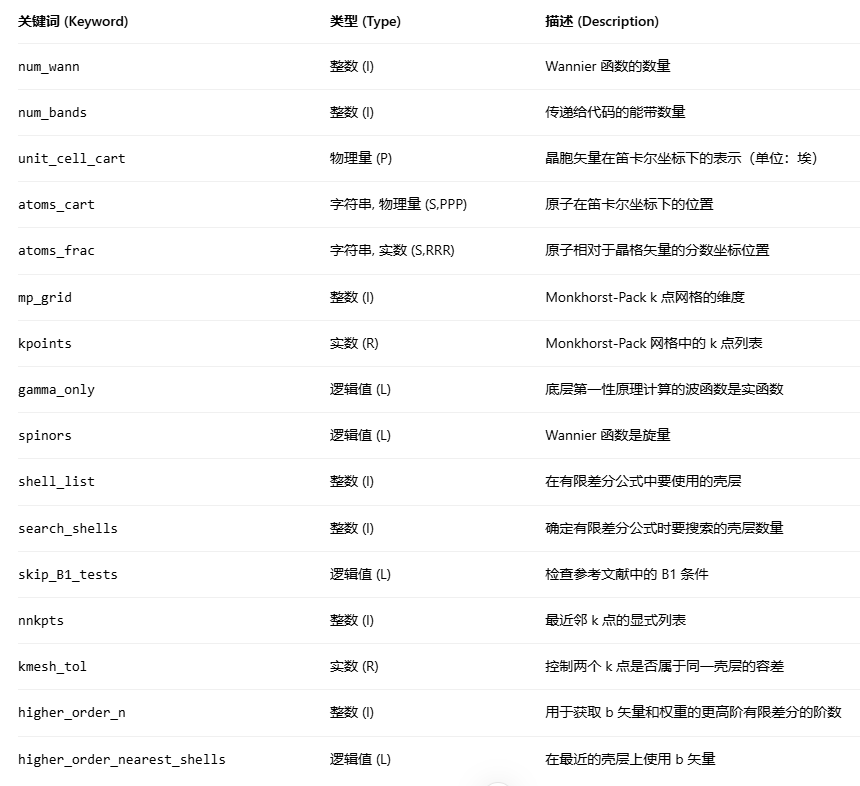
\includegraphics[max width=0.88\linewidth,max height=0.62\textheight,keepaspectratio]{assets/figure-d68f621e2425.png}
\end{figure}\par\par


seedname.win 文件关键词:系统定义\par


用于定义系统的 seedname.win文件关键词。参数类型表示为:I 代表整数,R 代表实数,P 代表物理量,L 代表逻辑值,S 代表文本字符串。\par


注意:在同一个输入文件中,不能同时定义 atoms\_\allowbreak{}cart和 atoms\_\allowbreak{}frac这两个关键词。\par


\subsubsection{任务控制参数}


\par\begin{figure}[H]\centering
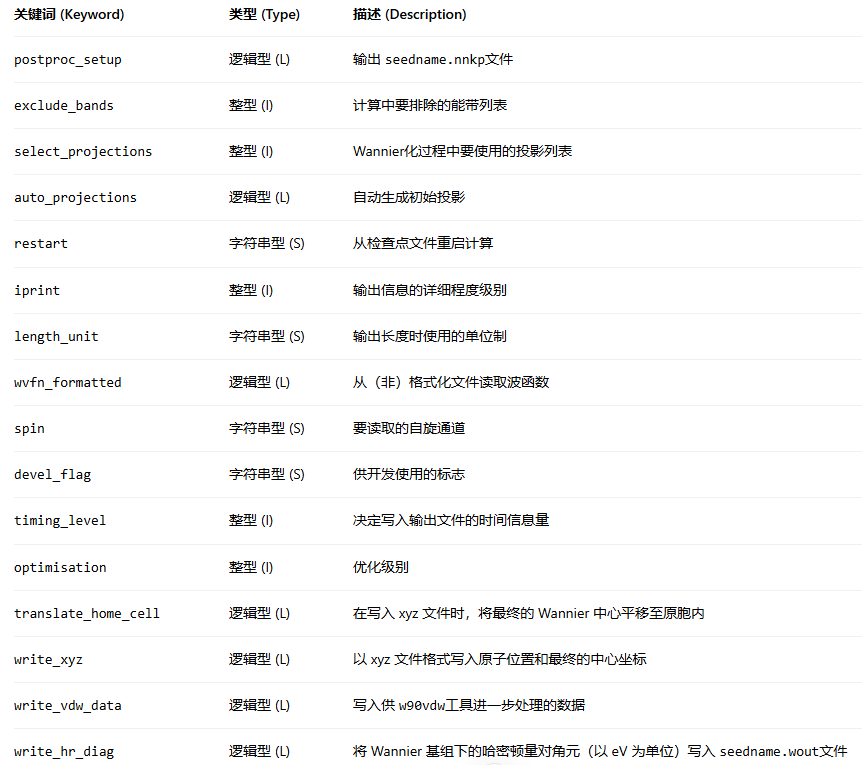
\includegraphics[max width=0.88\linewidth,max height=0.62\textheight,keepaspectratio]{assets/figure-6b241b232566.png}
\end{figure}\par\par


seedname.win 文件关键字:作业控制\par


用于定义作业控制的 seedname.win文件关键字。参数类型表示为:I 代表整数,R 代表实数,P 代表物理量,L 代表逻辑值,S 代表文本字符串。\par


注意:translate\_\allowbreak{}home\_\allowbreak{}cell仅在 write\_\allowbreak{}xyz为 .true.时相关。\par


\subsubsection{解纠缠参数}


\par\begin{figure}[H]\centering
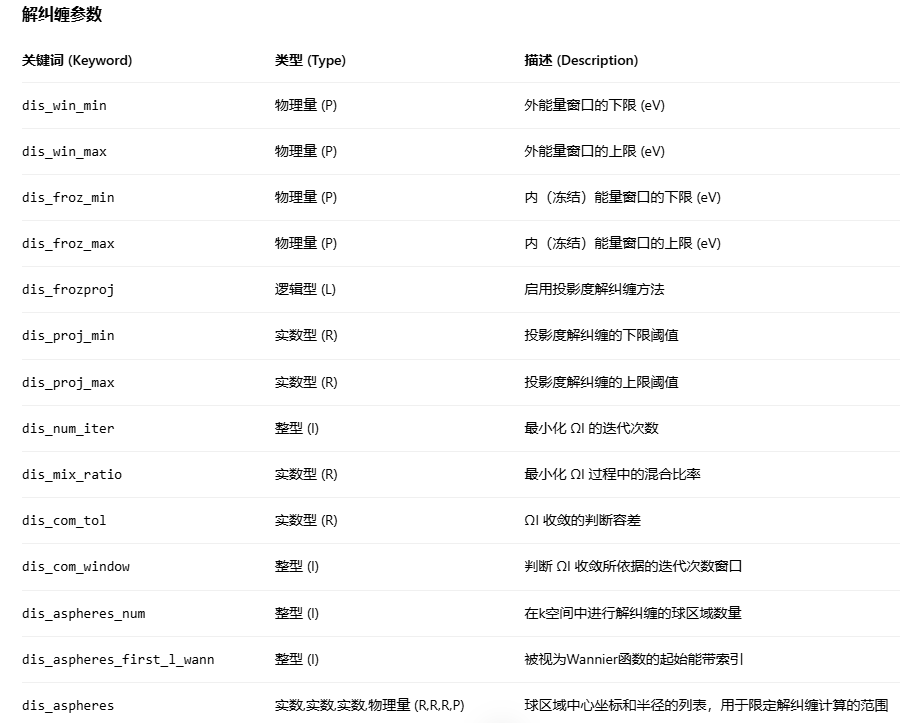
\includegraphics[max width=0.88\linewidth,max height=0.62\textheight,keepaspectratio]{assets/figure-939937979338.png}
\end{figure}\par\par


seedname.win 文件中控制解纠缠的关键字\par


关键字参数类型说明如下:\par


I 代表整数\par


R 代表实数\par


P 代表物理量\par


L 代表逻辑值\par


S 代表文本字符串\par


\subsubsection{优化参数}


\par\begin{figure}[H]\centering
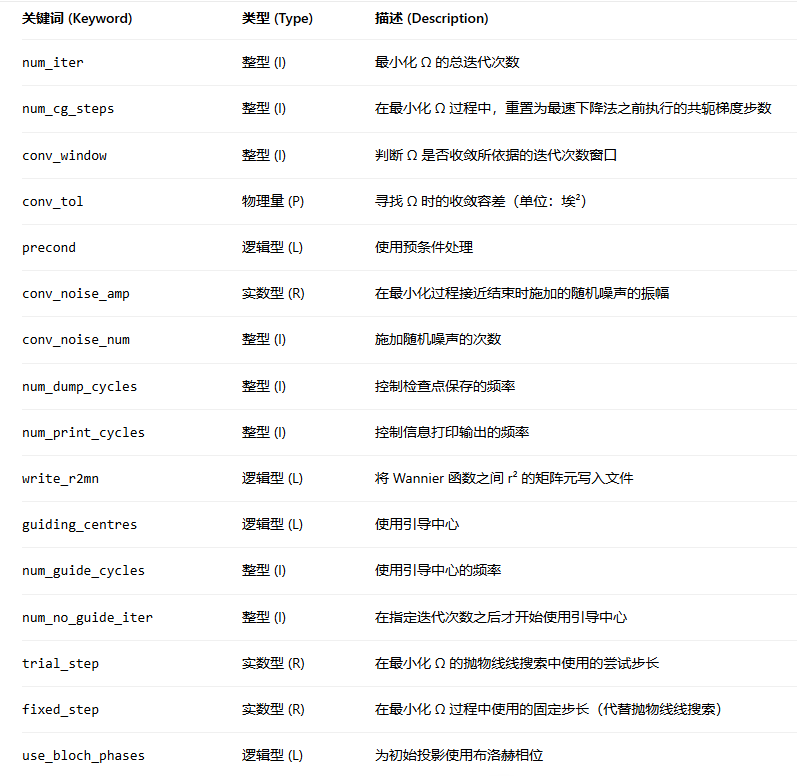
\includegraphics[max width=0.88\linewidth,max height=0.62\textheight,keepaspectratio]{assets/figure-e19a9c3456a8.png}
\end{figure}\par\par


\par\begin{figure}[H]\centering
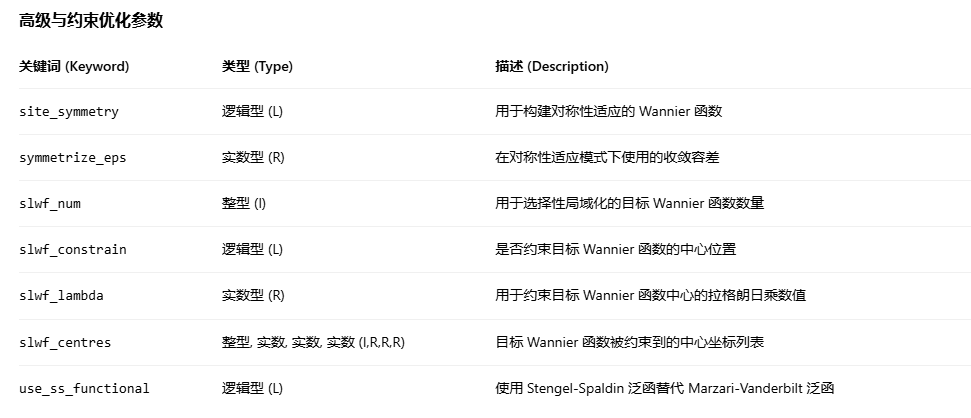
\includegraphics[max width=0.88\linewidth,max height=0.62\textheight,keepaspectratio]{assets/figure-99b81f5b40c8.png}
\end{figure}\par\par


L (Logical): 逻辑值(是/\allowbreak{}否)\par


R (Real): 实数\par


I (Integer): 整数\par


I,R,R,R: 表示需要提供一组参数,通常为一个整数(如函数索引)后跟三个实数(如空间坐标)\par


\par\begin{figure}[H]\centering
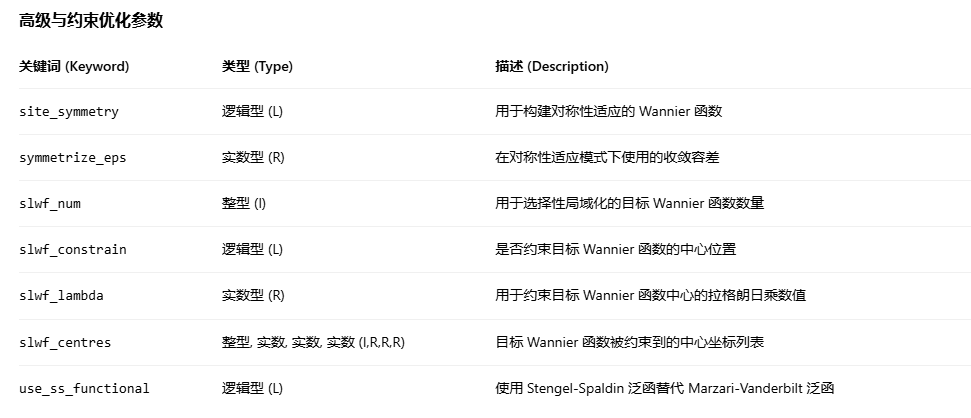
\includegraphics[max width=0.88\linewidth,max height=0.62\textheight,keepaspectratio]{assets/figure-99b81f5b40c8.png}
\end{figure}\par\par


\subsubsection{绘图参数}


\par\begin{figure}[H]\centering
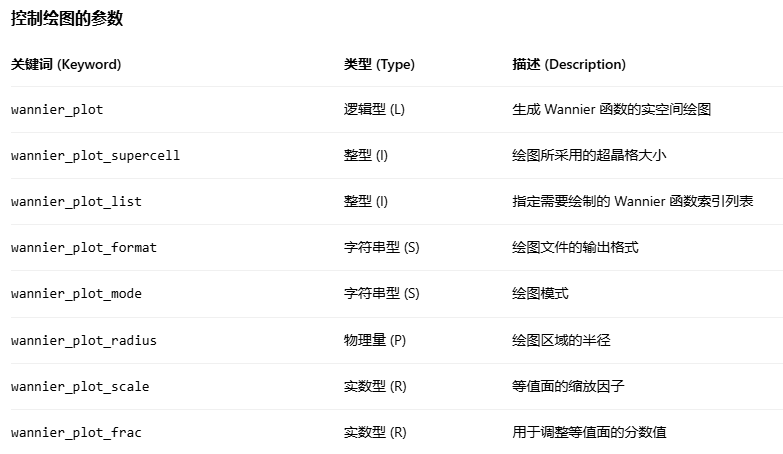
\includegraphics[max width=0.88\linewidth,max height=0.62\textheight,keepaspectratio]{assets/figure-d17082098141.png}
\end{figure}\par\par


\par\begin{figure}[H]\centering
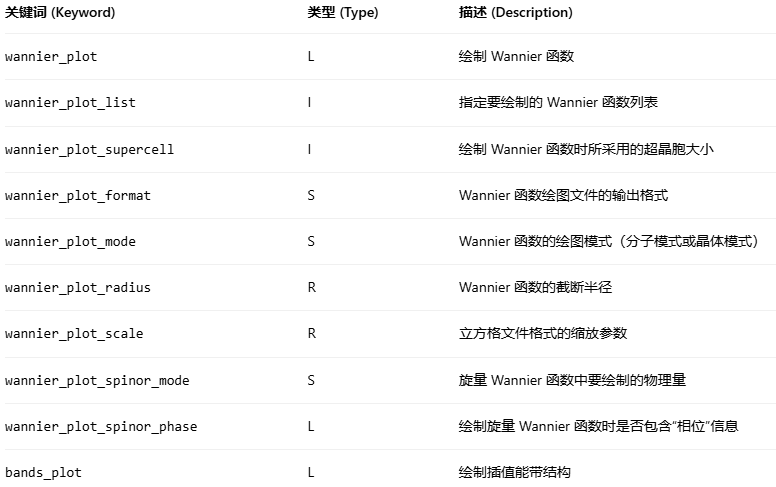
\includegraphics[max width=0.88\linewidth,max height=0.62\textheight,keepaspectratio]{assets/figure-06aa82188508.png}
\end{figure}\par\par


\par\begin{figure}[H]\centering
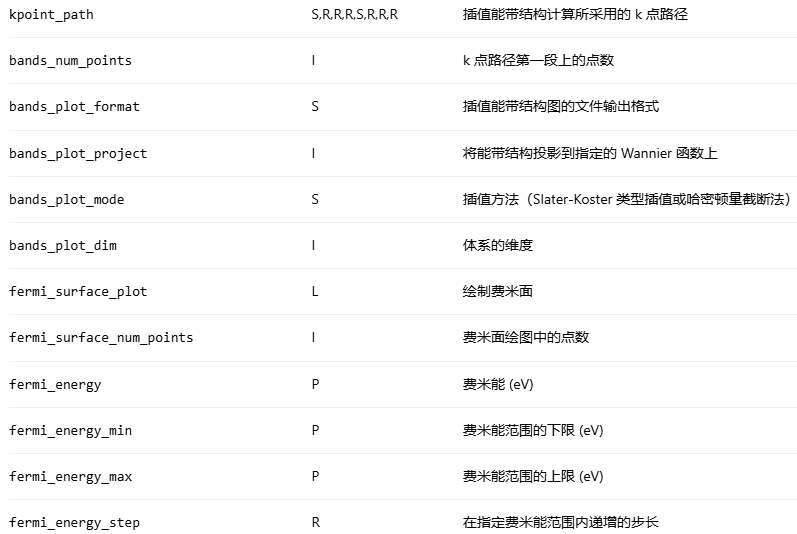
\includegraphics[max width=0.88\linewidth,max height=0.62\textheight,keepaspectratio]{assets/figure-717e1b16130f.png}
\end{figure}\par\par


\par\begin{figure}[H]\centering
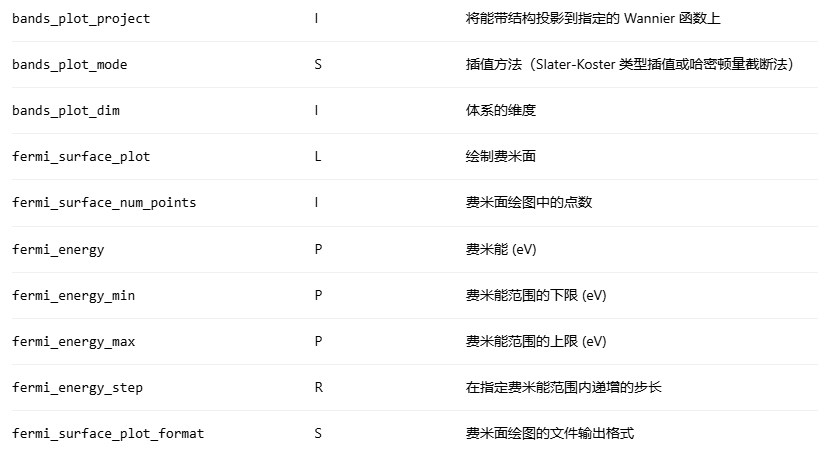
\includegraphics[max width=0.88\linewidth,max height=0.62\textheight,keepaspectratio]{assets/figure-4c9379ca045b.png}
\end{figure}\par\par


\par\begin{figure}[H]\centering
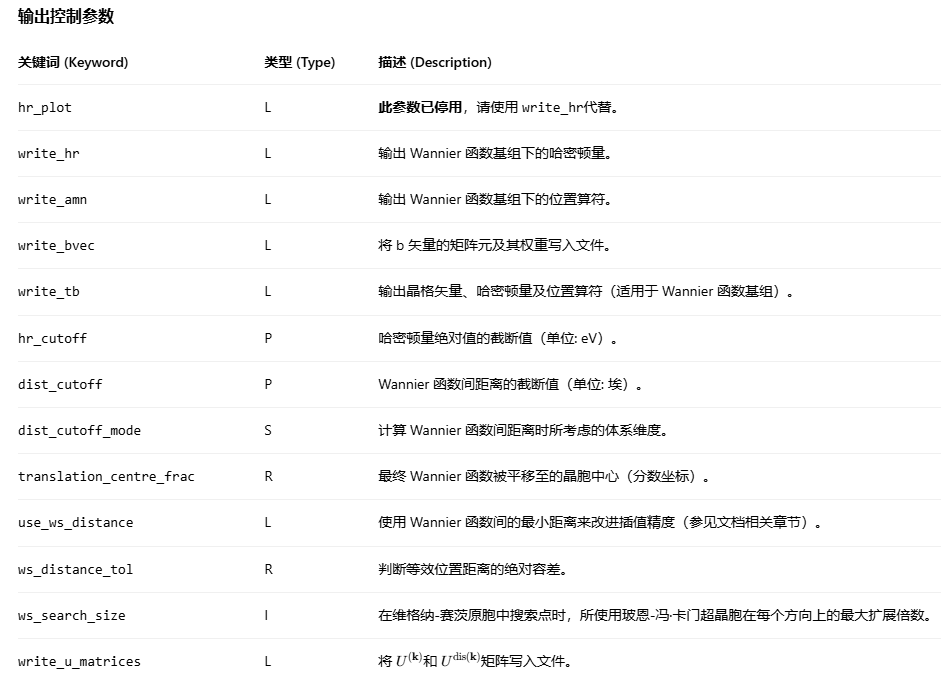
\includegraphics[max width=0.88\linewidth,max height=0.62\textheight,keepaspectratio]{assets/figure-b257c7deffc7.png}
\end{figure}\par\par


\subsubsection{输运参数}


\par\begin{figure}[H]\centering
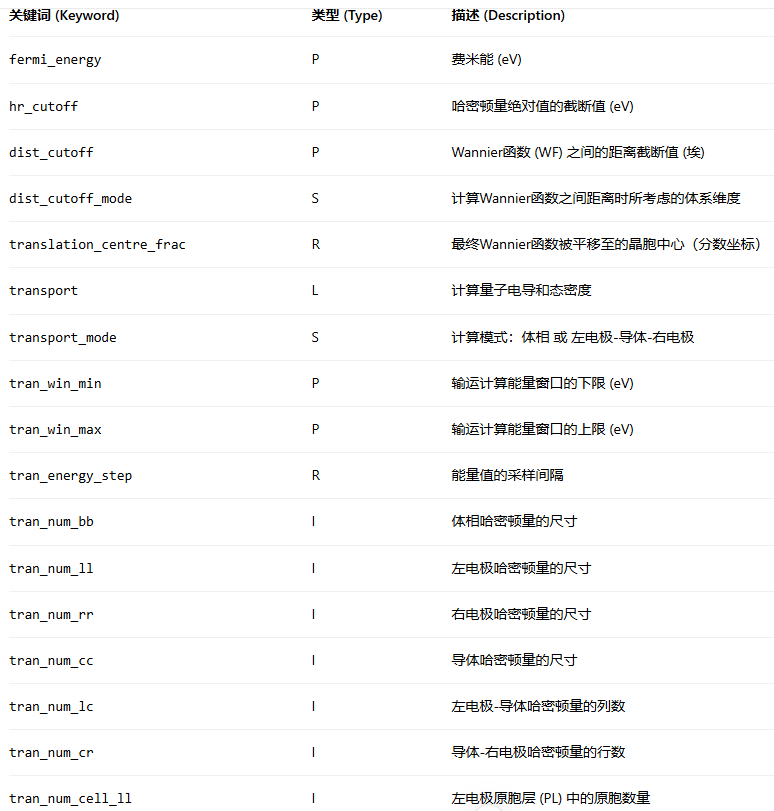
\includegraphics[max width=0.88\linewidth,max height=0.62\textheight,keepaspectratio]{assets/figure-4f56dec3909b.png}
\end{figure}\par\par


\par\begin{figure}[H]\centering
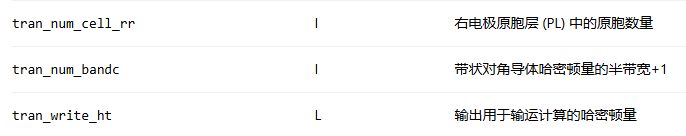
\includegraphics[max width=0.88\linewidth,max height=0.62\textheight,keepaspectratio]{assets/figure-94b15733933e.png}
\end{figure}\par\par


\par\begin{figure}[H]\centering
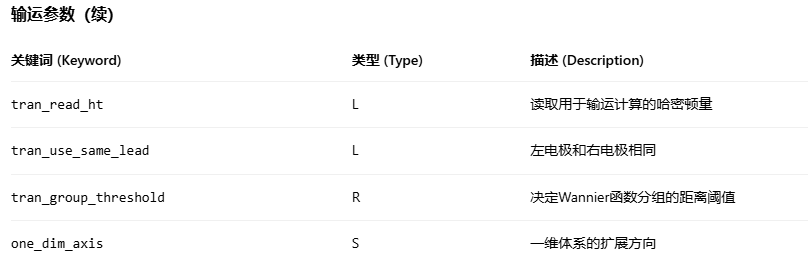
\includegraphics[max width=0.88\linewidth,max height=0.62\textheight,keepaspectratio]{assets/figure-5bedb082daa6.png}
\end{figure}\par\par



\section{以Bi烯为例的wannier90表面态计算}
\begin{articlemeta}
\textbf{日期：}2025-11-22\hfill\textbf{在线原文：}\href{https://marx2001.github.io/sci-note\_posts/20251122-Bi-m}{marx2001.github.io}
\end{articlemeta}

\subsubsection{心得笔记}


-免责声明:私人笔记-不传播 -原作者示例来源于公众号“计算凝聚态物理”,本笔记是用于学习、复现此公众号中的教程,并记录本人遇到的问题和步骤以及心得体会,如在互联网上检索到本文章,请勿用作他途。\par


注意,安装6.3.0版本以上的vasp,不包含6.3.0的vasp,并且编译的时候不要注释掉并行计算,wannier3.1.0版本是支持并行计算的,如果注释掉的话,会报错。\par


\subsubsection{1.能带计算}


计算得到BAND.dat,KLABELS,查看能带中的轨道贡献,通过投影能带,我们需要投影Bi原子的p轨道,原胞有两个原子,每个原子6个p轨道,我们需要拟合12个wannier轨道。\par


\par\begin{figure}[H]\centering
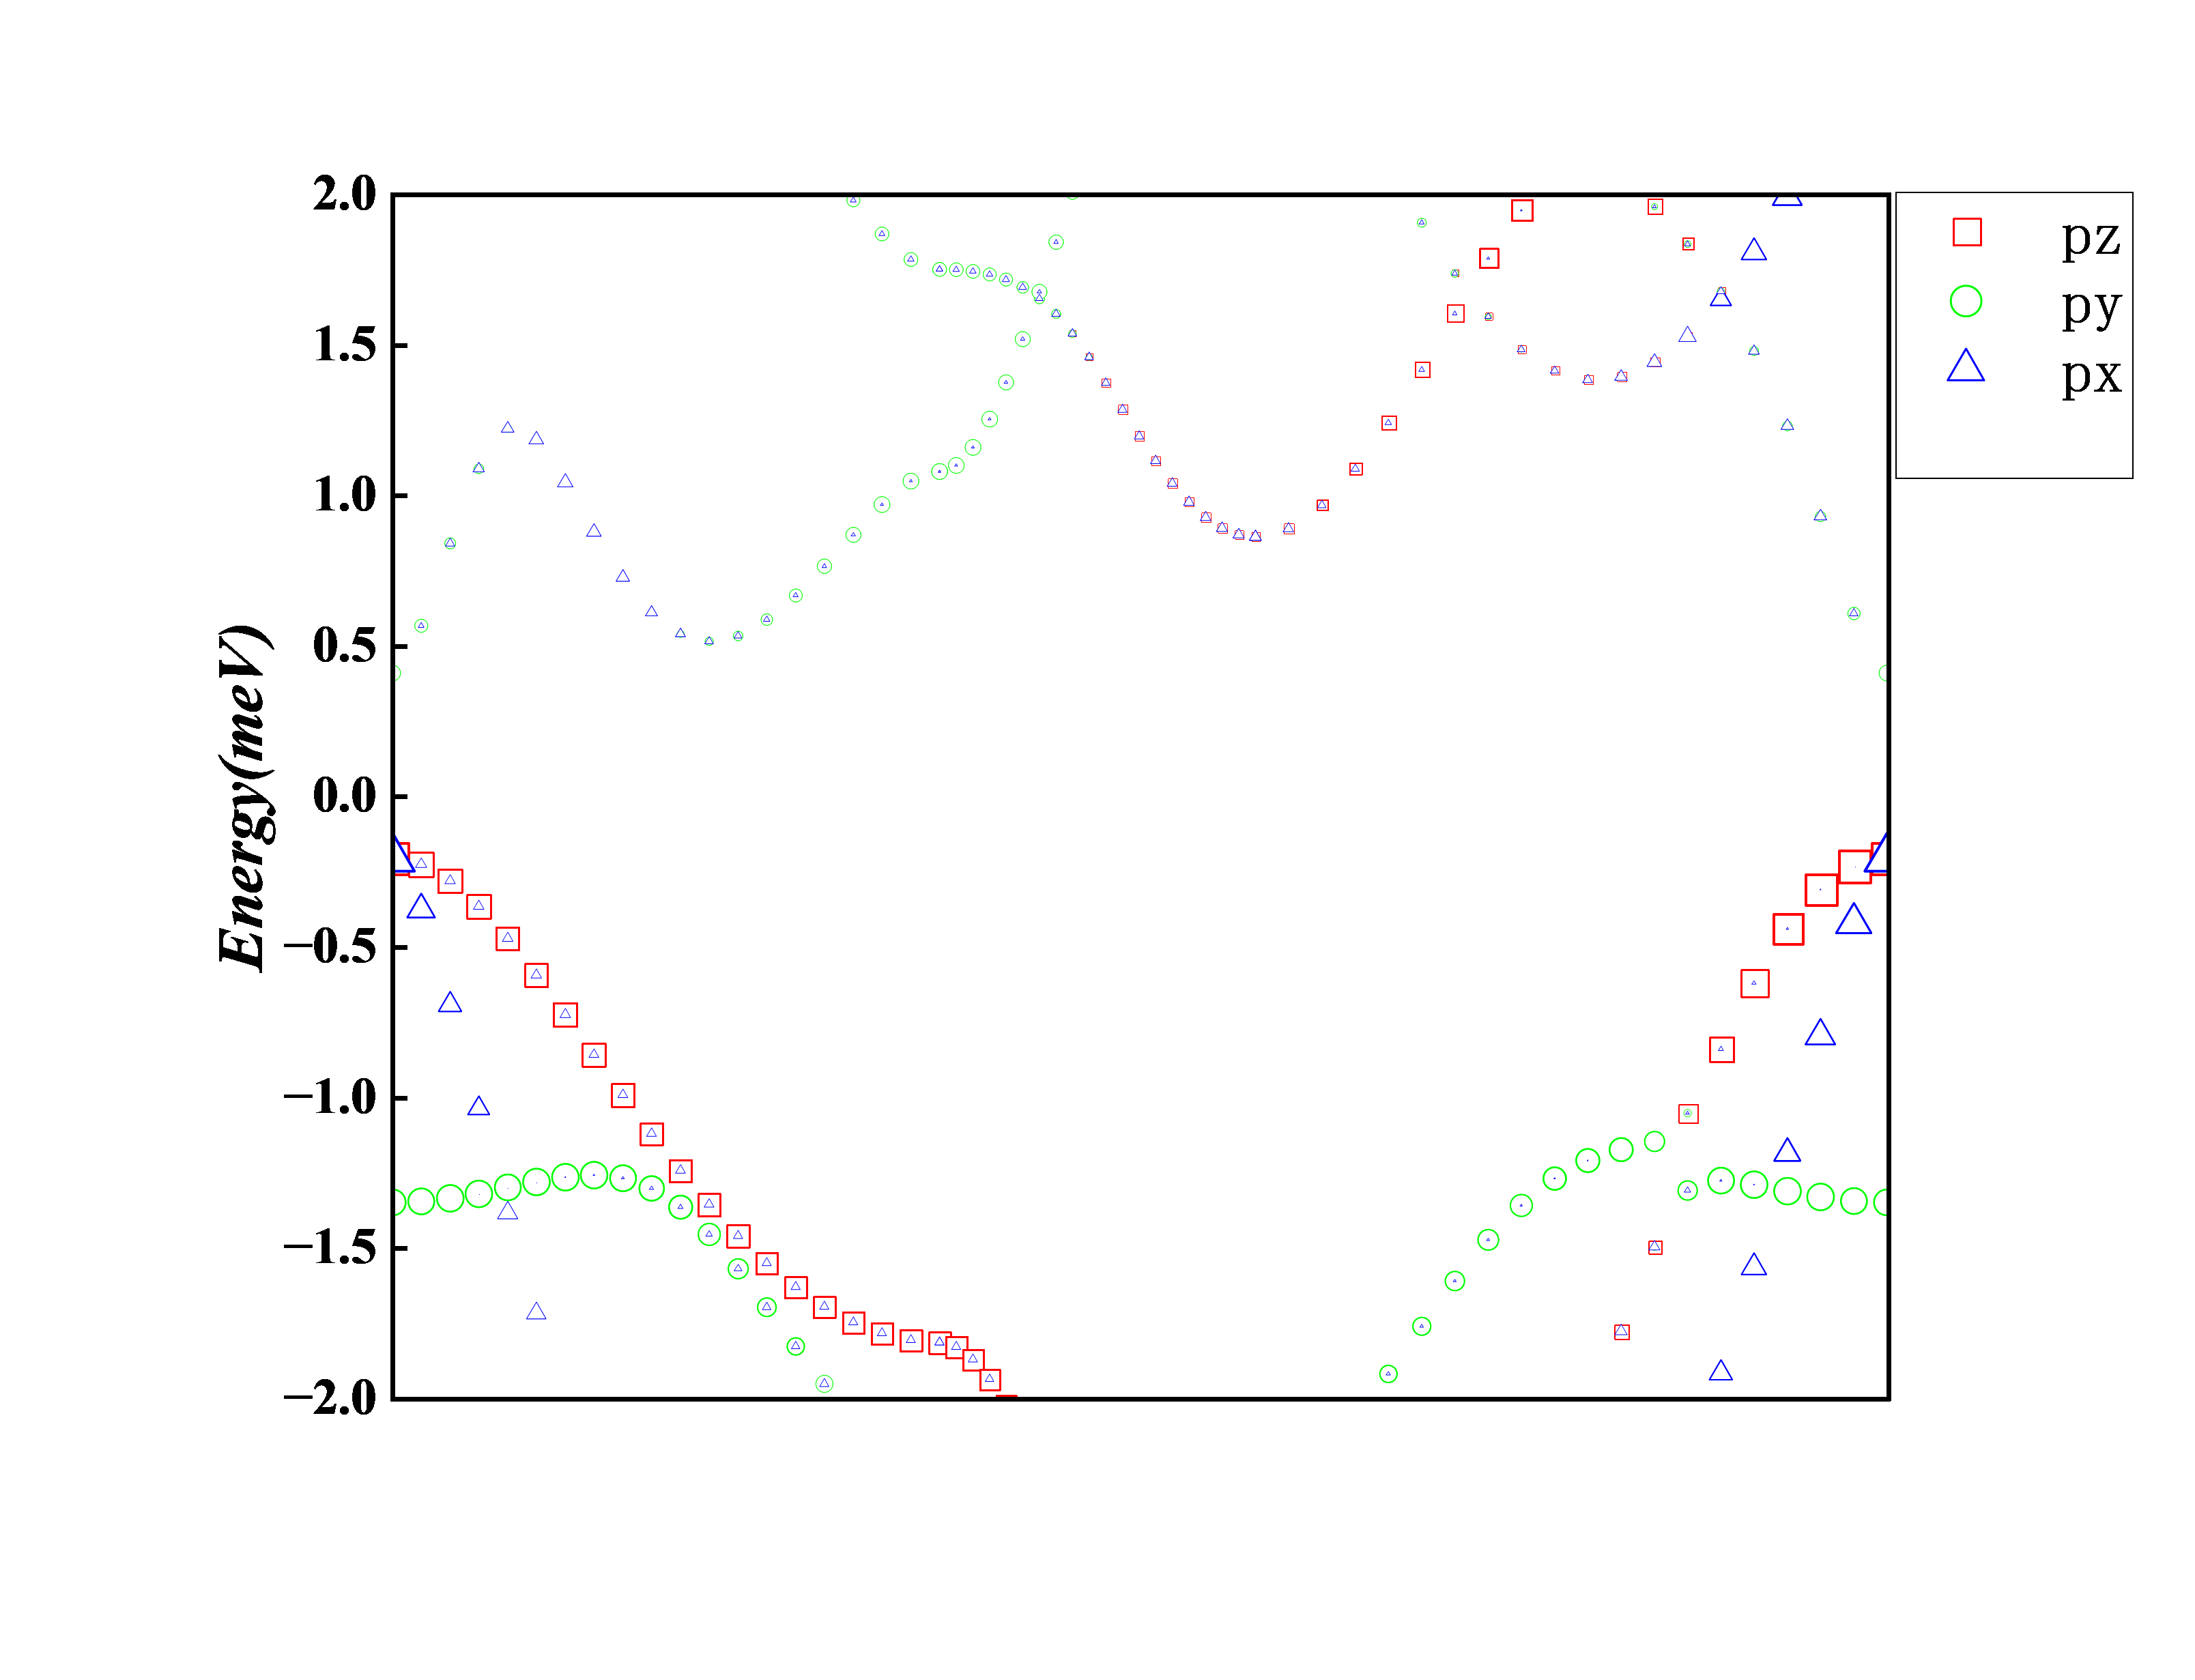
\includegraphics[max width=0.88\linewidth,max height=0.62\textheight,keepaspectratio]{assets/figure-8c9e3c280c9b.png}
\end{figure}\par\par


\par\begin{figure}[H]\centering
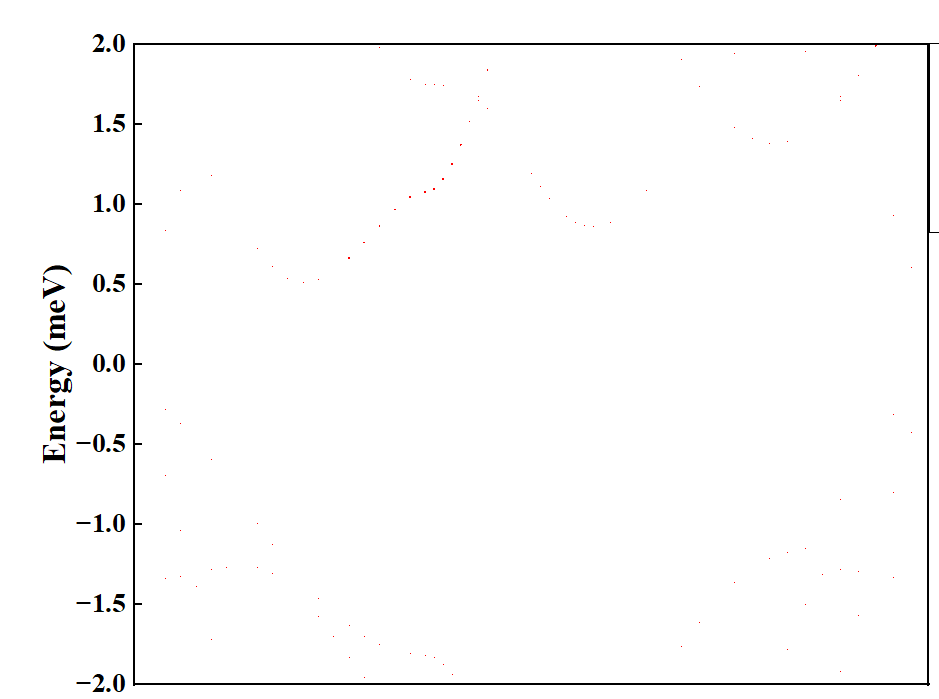
\includegraphics[max width=0.88\linewidth,max height=0.62\textheight,keepaspectratio]{assets/figure-957763f1635a.png}
\end{figure}\par\par


\subsubsection{2.静态自洽计算(注意添加LWANNIER90=.T)}


准备文件 
\par\begin{figure}[H]\centering
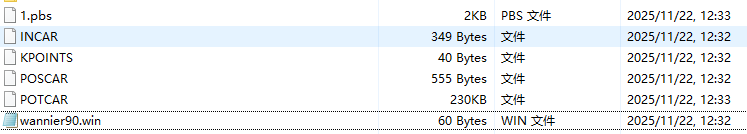
\includegraphics[max width=0.88\linewidth,max height=0.62\textheight,keepaspectratio]{assets/figure-dd2190b7d83c.png}
\end{figure}\par\par


win文件内容:\par


\begin{inlinecodebox}{命令示例 · shell}
\VerbatimInput[fontsize=\small,breaklines=true,breakanywhere=true,tabsize=2,listparameters={\setlength{\topsep}{0pt}\setlength{\partopsep}{0pt}\setlength{\parsep}{0pt}}]{code/009-001.sh}
\end{inlinecodebox}


NBANDS = 64(该数值应为 CPU 核心数的整数倍;此处使用 64 核提交),并在 INCAR 中加入 LWANNIER90 = T。\par


INCAR文件内容:\par


\begin{codeindexbox}{代码清单 A.9.2}
语言：shell；完整代码见附录第 \pageref{code:9:2} 页，共 30 行。
\end{codeindexbox}


\subsubsection{3.vasp非自洽计算,拟合Wannier90}


win文件中加入,同时修改ICHGCAR=11\par


\begin{codeindexbox}{代码清单 A.9.3}
语言：shell；完整代码见附录第 \pageref{code:9:3} 页，共 15 行。
\end{codeindexbox}


这个步骤需要反复调试能量窗口,如果成功的话,会产生新的文件。wannier90.amn, wannier90.eig, wannier90.mmn, wannier90.win, wannier90.wout\par


\subsubsection{4. Wannier90计算}


修改wannier90.win,上一步基础上,增加\par


\begin{codeindexbox}{代码清单 A.9.4}
语言：shell；完整代码见附录第 \pageref{code:9:4} 页，共 10 行。
\end{codeindexbox}


这里bands\_\allowbreak{}num\_\allowbreak{}points = 20 跟 VASPKIT 中能带计算的KPOINTS中 K 点数要相同(如下 KPOINTS的前三行,第二行中 K 点密度是 20,这么做是为了方便对比 VASP 和 wannier90 的能带)\par


提交wannier90的计算:\par


\begin{inlinecodebox}{命令示例 · shell}
\VerbatimInput[fontsize=\small,breaklines=true,breakanywhere=true,tabsize=2,listparameters={\setlength{\topsep}{0pt}\setlength{\partopsep}{0pt}\setlength{\parsep}{0pt}}]{code/009-005.sh}
\end{inlinecodebox}


\subsubsection{5.对比vasp和Wannier90的能带}


找到能带计算的费米能级:\par


\begin{inlinecodebox}{命令示例 · shell}
\VerbatimInput[fontsize=\small,breaklines=true,breakanywhere=true,tabsize=2,listparameters={\setlength{\topsep}{0pt}\setlength{\partopsep}{0pt}\setlength{\parsep}{0pt}}]{code/009-006.sh}
\end{inlinecodebox}


查看费米能级后,将能带计算的BAND.dat和KLABELS放到wannier90计算的文件夹中,修改compare\_\allowbreak{}wan\_\allowbreak{}vasp.py中的efermi,然后运行。\par


\subsubsection{6.WannierTools 计算边缘态和陈数}


\paragraph{(1) 边缘态}


以 zig-zag方向为例,展示计算得到的边界态 参照 wannier90.win 中的信息,修改wannierTools 的输入文件 wt.in:\par


\begin{codeindexbox}{代码清单 A.9.7}
语言：shell；完整代码见附录第 \pageref{code:9:7} 页，共 63 行。
\end{codeindexbox}


运行WannierTools:\par


\begin{inlinecodebox}{命令示例 · shell}
\VerbatimInput[fontsize=\small,breaklines=true,breakanywhere=true,tabsize=2,listparameters={\setlength{\topsep}{0pt}\setlength{\partopsep}{0pt}\setlength{\parsep}{0pt}}]{code/009-008.sh}
\end{inlinecodebox}


运行完后绘图:\par


\begin{inlinecodebox}{命令示例 · shell}
\VerbatimInput[fontsize=\small,breaklines=true,breakanywhere=true,tabsize=2,listparameters={\setlength{\topsep}{0pt}\setlength{\partopsep}{0pt}\setlength{\parsep}{0pt}}]{code/009-009.sh}
\end{inlinecodebox}


\par\begin{figure}[H]\centering
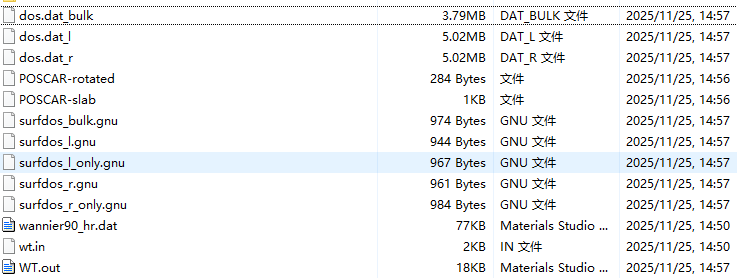
\includegraphics[max width=0.88\linewidth,max height=0.62\textheight,keepaspectratio]{assets/figure-81bd9174f5c1.png}
\end{figure}\par\par


我复现的边缘态:\par


\par\begin{figure}[H]\centering
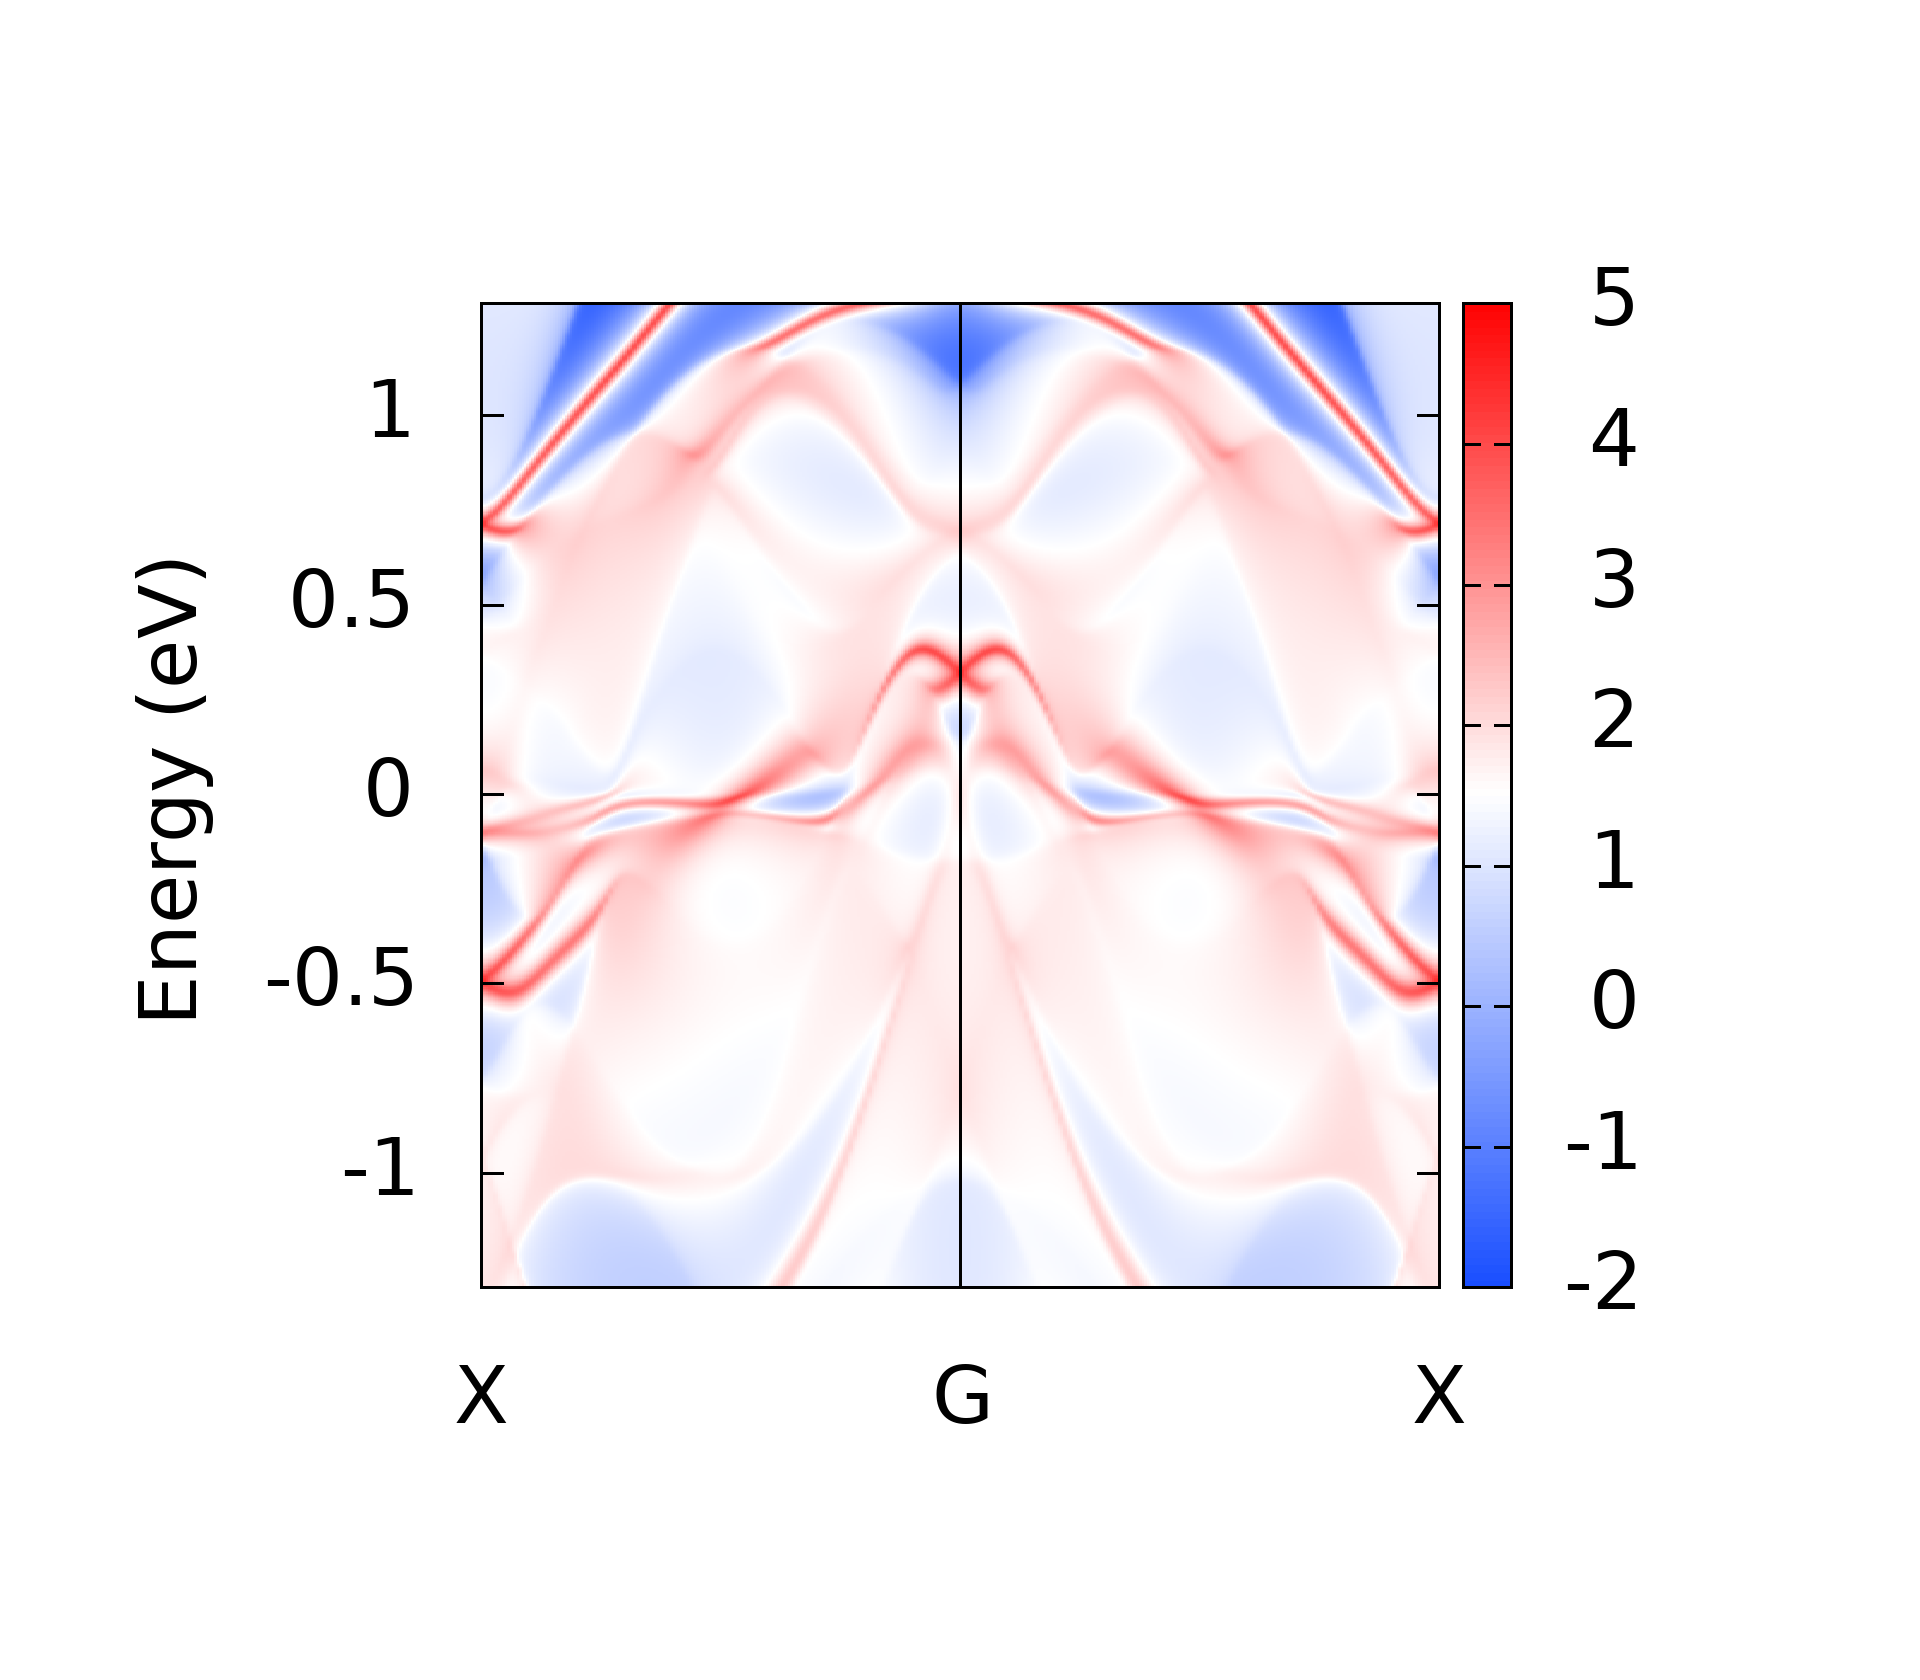
\includegraphics[max width=0.88\linewidth,max height=0.62\textheight,keepaspectratio]{assets/figure-8a3462a72310.png}
\end{figure}\par\par


与公众号的文件不同,很奇怪,但原因应该是我的拟合的轨道不同,我设置的Bi:l=1\par


一些可能的原因:我的NBANDS设置是64,而示例中是40,导致我的拟合能带和DFT能带有一些差距。这个保持质疑,我始终按照博主给的INCAR进行计算,但是始终得不到和公众号一样的带隙。开 ISPIN会让费米能级升高。加入下面tag后,费米能级继续升高:\par


\begin{inlinecodebox}{命令示例 · shell}
\VerbatimInput[fontsize=\small,breaklines=true,breakanywhere=true,tabsize=2,listparameters={\setlength{\topsep}{0pt}\setlength{\partopsep}{0pt}\setlength{\parsep}{0pt}}]{code/009-010.sh}
\end{inlinecodebox}


开SOC后,费米能级上升了\par


不用管了,不知道是什么原因,导致的费米能级无法复现,我们只需要知道整体步骤即可:\par


使用由VASP生成的 wannier90.amn、wannier90.mmn、wannier90.eig和 wannier90.win文件,生成最大局域瓦尼尔函数。\par


在后台运行Wannier90,命令为:wannier90.x wannier90 \&。\par


这将生成一系列文件,我们所需的是 wannier90.chk(检查点文件)。\par


使用得到的瓦尼尔函数计算体材料的能带结构,并将其与通过DFT计算得到的能带进行比较。\par


将步骤1中得到的 wannier90.chk和 wannier90.eig文件复制到当前文件夹,在后台运行Wannier90,命令为:wannier90.x wannier90 \&。\par


执行命令 gnuplot –persist wannier90\_\allowbreak{}band.gnu来绘制能带结构图。\par


将瓦尼尔方法计算得到的能带结构与DFT计算的结果进行比较。\par


使用得到的瓦尼尔函数来获取瓦尼尔哈密顿量。\par


将步骤1中得到的 wannier90.chk和 wannier90.eig文件复制到当前文件夹,在后台运行Wannier90,命令为:wannier90.x wannier90 \&。\par


检查输出文件 wannier90\_\allowbreak{}hr.dat。\par


计算表面态:\par


cp wt\_\allowbreak{}SS.in wt.in\par


wt.x \&\par


\begin{codeindexbox}{代码清单 A.9.11}
语言：shell；完整代码见附录第 \pageref{code:9:11} 页，共 63 行。
\end{codeindexbox}


\paragraph{(2) Z2计算}


计算威尔逊环(Wilson loop)和Z2拓扑不变量。\par


将 wannier90\_\allowbreak{}hr.dat从 5\_\allowbreak{}wannier\_\allowbreak{}cal目录的最后一步复制到此处。\par


将 wt\_\allowbreak{}Z2.in复制为 wt.in。\par


执行命令 wt.x \&来计算 Z2 拓扑不变量。\par


执行命令 gnuplot wanniercenter3D\_\allowbreak{}Z2.gnu来查看瓦尼尔电荷中心的演化。\par


检查 WT.out输出文件和 wanniercenter3D\_\allowbreak{}Z2.eps图像文件。\par


计算表面态。\par


将瓦尼尔计算步骤中的 wannier90\_\allowbreak{}hr.dat文件复制到此处。\par


将 wt\_\allowbreak{}SS.in复制为 wt.in。\par


执行命令 wt.x \&来计算表面态。\par


执行命令 gnuplot surfdos\_\allowbreak{}r.gnu来绘制表面态图谱。\par


检查 surfdos\_\allowbreak{}r.png图像文件。\par


完整的执行流程我已经fork到我的github库内,此处为基本的笔记指导,方便查阅。下方为基本的示例输入文件:\par


计算Z2\par


cp wt\_\allowbreak{}Z2.in wt.in\par


wt.x \&\par


\begin{codeindexbox}{代码清单 A.9.12}
语言：shell；完整代码见附录第 \pageref{code:9:12} 页，共 57 行。
\end{codeindexbox}


\subsubsection{报错:}


—————————————————————————– | \_\allowbreak{} \textbf{\_\allowbreak{}\_\allowbreak{} \_\allowbreak{} \_\allowbreak{} \_\allowbreak{}\_\allowbreak{}}\_\allowbreak{} \_\allowbreak{} | | | | | \_\allowbreak{} \textbackslash{}\allowbreak{} | | | | /\allowbreak{} \textbf{\_\allowbreak{}\_\allowbreak{}| | | | | | | | |\emph{) | | | | | | | \_\allowbreak{}\_\allowbreak{} | | | | |}| | \_\allowbreak{} < | | | | | | |\_\allowbreak{} | |\emph{| | | \_\allowbreak{} | |}) | | |}| | | |\textbf{| | \_\allowbreak{} | | (\emph{) |}}\emph{/\allowbreak{} \_\allowbreak{}}\textbf{/\allowbreak{} \_\allowbreak{}}\emph{\_\allowbreak{}| (}) | | | | internal error in: mkpoints\_\allowbreak{}change.F at line: 794 | | | | internal error in GENERATE\_\allowbreak{}KPOINTS\_\allowbreak{}TRANS: number of G-vector | | changed in star 7778 7776 | | | | If you are not a developer, you should not encounter this problem. | | Please submit a bug report. | | | —————————————————————————–\par


k点取偶数即可规避。\par


\begin{inlinecodebox}{命令示例 · shell}
\VerbatimInput[fontsize=\small,breaklines=true,breakanywhere=true,tabsize=2,listparameters={\setlength{\topsep}{0pt}\setlength{\partopsep}{0pt}\setlength{\parsep}{0pt}}]{code/009-013.sh}
\end{inlinecodebox}


退出环境\par



\section{wannier90汇总}
\begin{articlemeta}
\textbf{日期：}2025-11-23\hfill\textbf{在线原文：}\href{https://marx2001.github.io/sci-note\_posts/20251123}{marx2001.github.io}
\end{articlemeta}

\subsubsection{心得笔记}


拟合完的指令:wannier90.x wannier90 \& 激活TB2J:source /\allowbreak{}public/\allowbreak{}home/\allowbreak{}cssong/\allowbreak{}song/\allowbreak{}zhchen/\allowbreak{}1\_\allowbreak{}materials/\allowbreak{}1\_\allowbreak{}VTeCl/\allowbreak{}TB2J/\allowbreak{}strain/\allowbreak{}-2/\allowbreak{}TB2J\_\allowbreak{}env/\allowbreak{}bin/\allowbreak{}activate 进入pyw90环境:conda activate pyw90\_\allowbreak{}env pyw90 eig suggest –path . -e -20 20 -w 20 在选定能量区间内计算推荐的内外能量窗口的范围\par


求平均值:TB2J\_\allowbreak{}merge.py –type structure x y z\par


求磁耦合参数:wann2J.py –spinor –groupby spin –efermi -1.0098 –emin -2.06514 –emax -0.065 –elements Nb –kmesh 9 9 1 –nz 100 –rcut 6.0 –np 1 第一次测试\par


安装计算SHC的环境:conda install -c conda-forge wannierberri numpy scipy matplotlib h5py sympy -y\par


计算自旋霍尔电导:postw90.x wannier90\par



\section{Wannier90的表面态的参数选择标准1\_\allowbreak{}示例文件的参数注释}
\begin{articlemeta}
\textbf{日期：}2025-11-25\hfill\textbf{在线原文：}\href{https://marx2001.github.io/sci-note\_posts/20251125-wannier-in-mrx}{marx2001.github.io}
\end{articlemeta}

计算表面态\par


\begin{codeindexbox}{代码清单 A.11.1}
语言：shell；完整代码见附录第 \pageref{code:11:1} 页，共 63 行。
\end{codeindexbox}


\subsubsection{参数选择标准}


\begin{codeindexbox}{代码清单 A.11.2}
语言：shell；完整代码见附录第 \pageref{code:11:2} 页，共 10 行。
\end{codeindexbox}


\par\begin{figure}[H]\centering
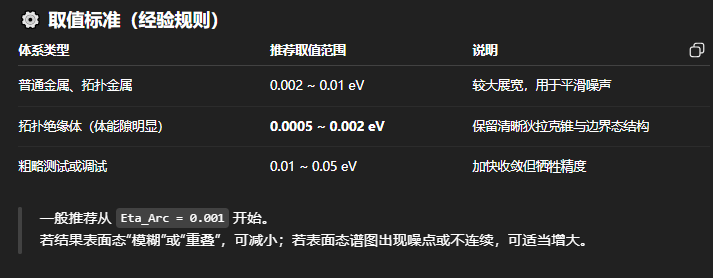
\includegraphics[max width=0.88\linewidth,max height=0.62\textheight,keepaspectratio]{assets/figure-93553ef48545.png}
\end{figure}\par\par


\par\begin{figure}[H]\centering
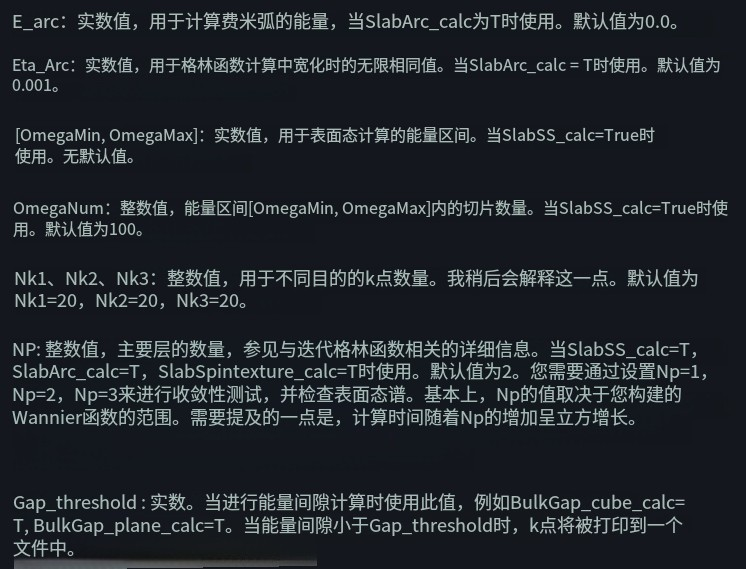
\includegraphics[max width=0.88\linewidth,max height=0.62\textheight,keepaspectratio]{assets/figure-3a6eb4abd762.png}
\end{figure}\par\par


\par\begin{figure}[H]\centering
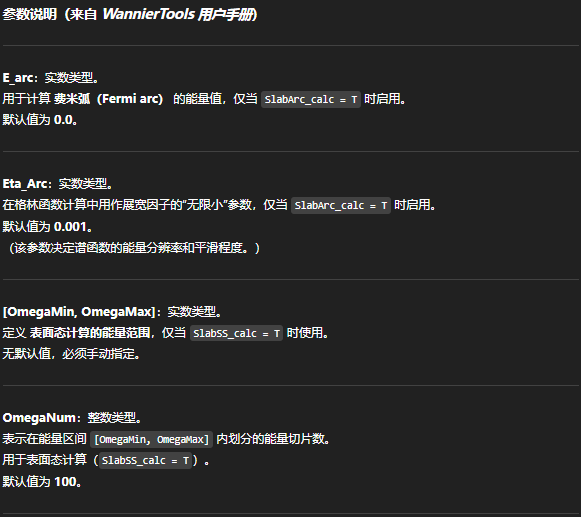
\includegraphics[max width=0.88\linewidth,max height=0.62\textheight,keepaspectratio]{assets/figure-e0c00fdc4437.png}
\end{figure}\par\par


\par\begin{figure}[H]\centering
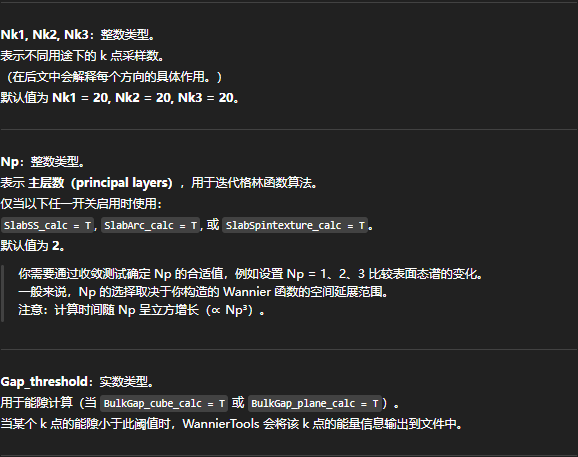
\includegraphics[max width=0.88\linewidth,max height=0.62\textheight,keepaspectratio]{assets/figure-861a0204850f.png}
\end{figure}\par\par


\begin{codeindexbox}{代码清单 A.11.3}
语言：shell；完整代码见附录第 \pageref{code:11:3} 页，共 4 行。
\end{codeindexbox}


\par\begin{figure}[H]\centering
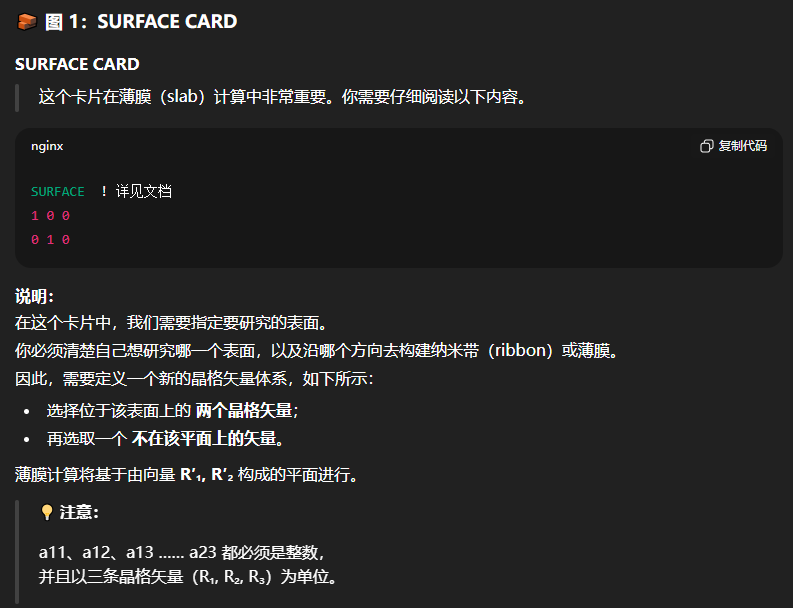
\includegraphics[max width=0.88\linewidth,max height=0.62\textheight,keepaspectratio]{assets/figure-ca8bf78846ff.png}
\end{figure}\par\par


\par\begin{figure}[H]\centering
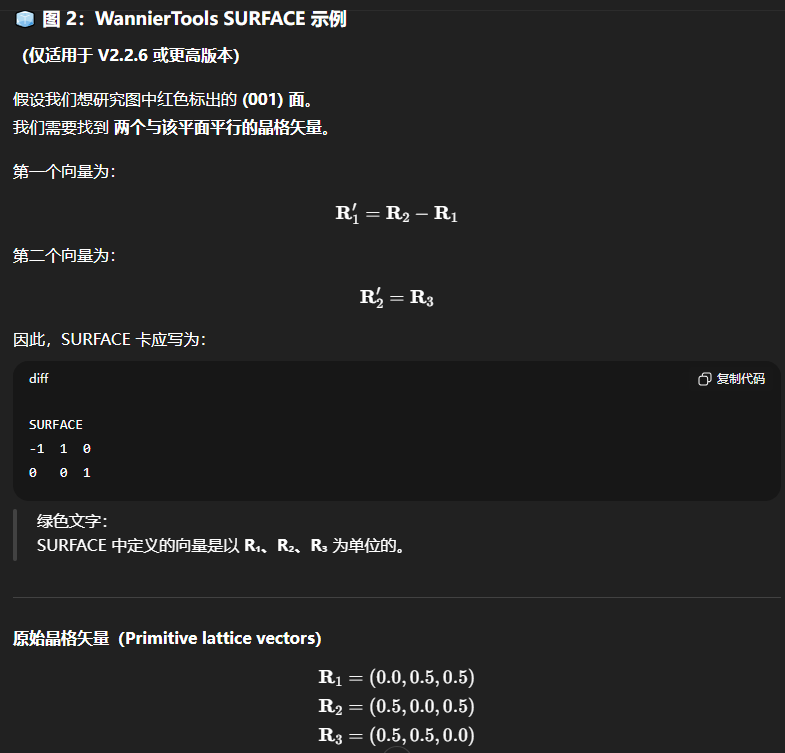
\includegraphics[max width=0.88\linewidth,max height=0.62\textheight,keepaspectratio]{assets/figure-c7643dd228cd.png}
\end{figure}\par\par


\par\begin{figure}[H]\centering
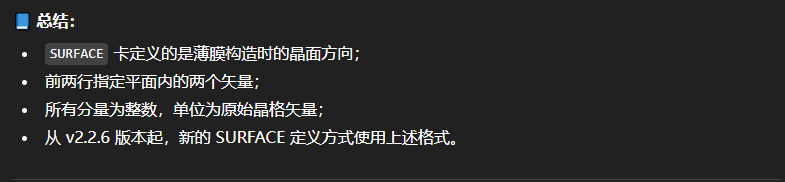
\includegraphics[max width=0.88\linewidth,max height=0.62\textheight,keepaspectratio]{assets/figure-791977fbbe37.png}
\end{figure}\par\par


\begin{codeindexbox}{代码清单 A.11.4}
语言：shell；完整代码见附录第 \pageref{code:11:4} 页，共 5 行。
\end{codeindexbox}


\par\begin{figure}[H]\centering
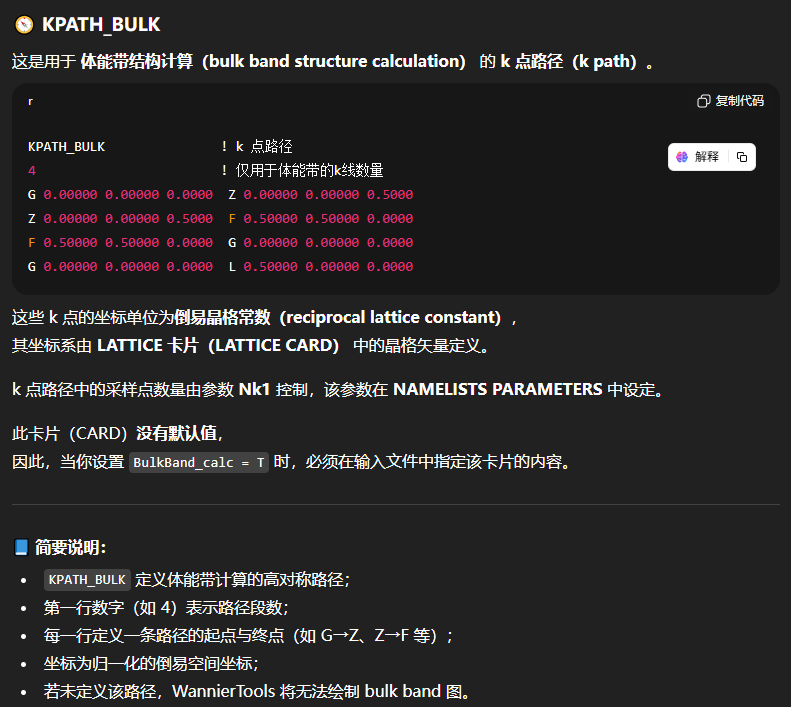
\includegraphics[max width=0.88\linewidth,max height=0.62\textheight,keepaspectratio]{assets/figure-322e9c50b9e5.png}
\end{figure}\par\par


\begin{codeindexbox}{代码清单 A.11.5}
语言：shell；完整代码见附录第 \pageref{code:11:5} 页，共 4 行。
\end{codeindexbox}


\par\begin{figure}[H]\centering
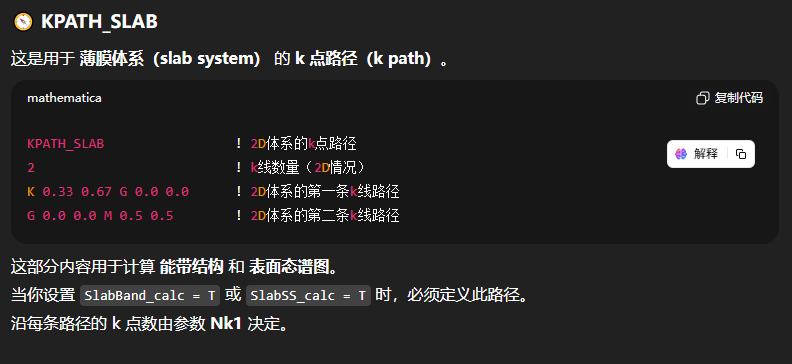
\includegraphics[max width=0.88\linewidth,max height=0.62\textheight,keepaspectratio]{assets/figure-0ed857ccb543.png}
\end{figure}\par\par


\par\begin{figure}[H]\centering
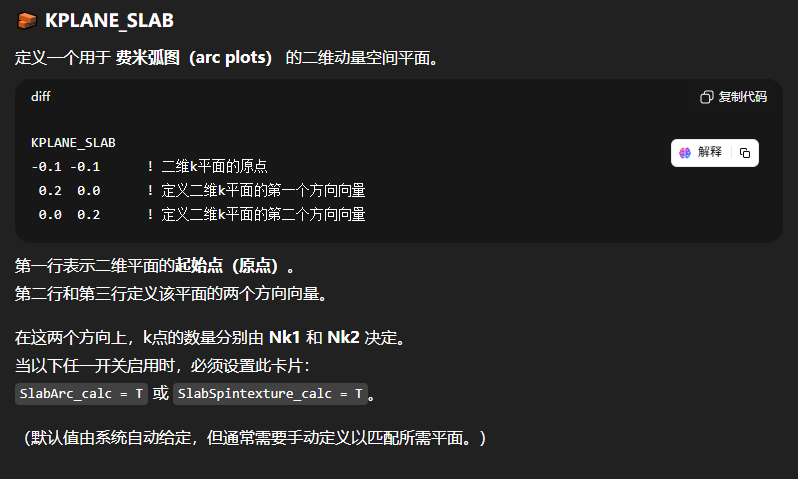
\includegraphics[max width=0.88\linewidth,max height=0.62\textheight,keepaspectratio]{assets/figure-9e58e4077a7f.png}
\end{figure}\par\par


\par\begin{figure}[H]\centering
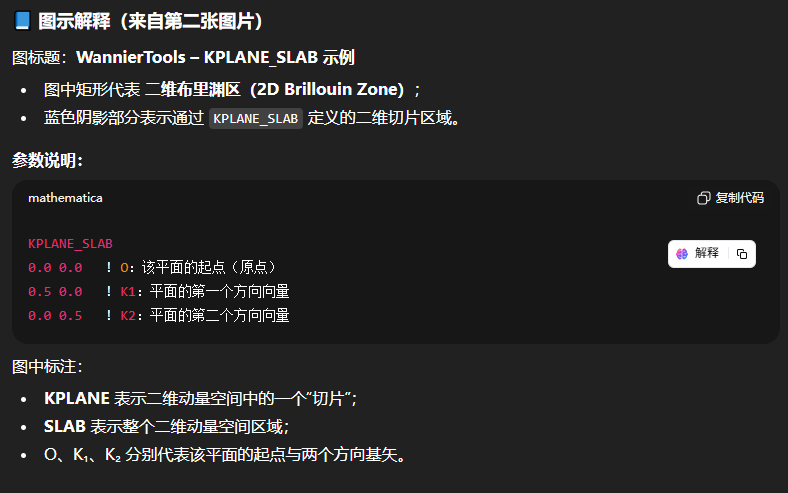
\includegraphics[max width=0.88\linewidth,max height=0.62\textheight,keepaspectratio]{assets/figure-13ad9960b5f4.png}
\end{figure}\par\par



\section{wannier90编译}
\begin{articlemeta}
\textbf{日期：}2025-11-25\hfill\textbf{在线原文：}\href{https://marx2001.github.io/sci-note\_posts/20251125}{marx2001.github.io}
\end{articlemeta}

\subsubsection{大概流程}


复制vasp6.4.3\par


tar-xvf vasp6.4.3 tar.gz\par


cp 配置文件到wannier90 3.1.0文件夹\par


cp make.inc\par


检查编译器路径并复制\par


nano make.inc文件,改LIBDIR到自己的mkl文件中\par


键入make all 开始安装(wannier90 3.1.0文件夹中)\par


makefile.include(这个是arch文件夹中的一个文件要复制出来然后修改成这个名称)。修改Wannier\_\allowbreak{}ROOT等内容以及LLIBS\par


安装vasp\par


make all\par



\section{以Bi烯为例的wannier90表面态计算}
\begin{articlemeta}
\textbf{日期：}2025-11-25\hfill\textbf{在线原文：}\href{https://marx2001.github.io/sci-note\_posts/20251125-wannier90-mrx}{marx2001.github.io}
\end{articlemeta}

\subsubsection{我的一些问题——AI回答,谨慎甄别}


AI引擎:Chatgpt-5.1 Auto决定回答时长\par


Q1:什么是wannier90?\par


A1: Wannier90 是一个在计算材料科学和凝聚态物理中非常重要的软件包,用于构造 Maximally Localized Wannier Functions(MLWFs,最大局域化的Wannier函数)。它是第一性原理计算中连接 电子能带结构 与 实空间局域化电子态 的关键工具。 固体物理中,电子波函数通常以Bloch波函数的形式表示,适用于周期性晶体。但bloch函数是在动量空间局域,实空间扩展,不适合描述化学键或者局域电子特性。\par


Wannier函数相反,它是实空间局域化的波函数。\par


Wannier90是一个独立的后处理程序,可以从多种第一性原理计算程序,导入计算结果,构造Wannier函数。\par


Q2:具体应用?\par


A1:拓扑绝缘体与陈绝缘体分析、电输运与自旋输运、光学响应与Berry相计算、紧束缚模型参数提取、分子吸附、磁性、超导配对分析\par


\subsubsection{表面态相关疑问}


Q1:拓扑绝缘体、高阶拓扑绝缘体以及表面态都是什么?\par


A1:拓扑绝缘体是一类内部(体)为绝缘体、表面为导体的量子态。其本质是:能带结构具有非平庸拓扑性质(即,无法连续变形为普通绝缘体),由 拓扑不变量(如 Z2、Chern数)区分。电子结构特征:体态 (bulk):具有能隙(如普通绝缘体);表面态(surface state):存在受保护的导电态;能带倒转(band inversion):由于强自旋轨道耦合(SOC),价带与导带在能量序上“翻转”,产生拓扑非平庸结构。可以理 解为:“内部像绝缘体,表皮却像金属。”\par


Q2:为什么计算二维体系的表面态,要计算bulk 能带呢?二维体系的是否具有不同面?(wt.in文件中要规定切面,且我遇见过6个切面都存在陈数的情况)\par


A2:这其实触及到了拓扑能带理论的核心逻辑:体态拓扑决定边界态。表面态(或边界态)来源于体态拓扑性质:拓扑材料的一个核心定理是:Bulk–Boundary Correspondence(体–边对应原理)。一个体态系统的拓扑不变量(如 Chern 数、Z2 指标)决定了其边界是否存在稳定的表面态。换句话说:表面态不是独立存在的;它是体能带(bulk band)拓扑结构的“投影”或“表现形式”。所以计算二维表面态的第一步是:确定 bulk 能带及其拓扑不变量。\par


1 从 DFT/\allowbreak{}Wannier90 得到 bulk 哈密顿矩阵 (wannier90\_\allowbreak{}hr.dat)\par


2 WannierTools 读取 bulk 哈密顿量\par


3 根据用户定义的表面切面 (surface plane),对晶格进行投影\par


4 构造 slab(超胞体)或半无限格林函数\par


5 求解表面态或边缘态谱\par


虽然二维体系在物理空间中厚度极薄,但它依然是一个晶格周期性的二维平面。 在WannierTools的框架中,二维系统仍被视为一个二维晶体中的周期性布洛赫体,因此在数值模拟时可以“虚拟地”切割出不同的边界方向。\par


\par\begin{figure}[H]\centering
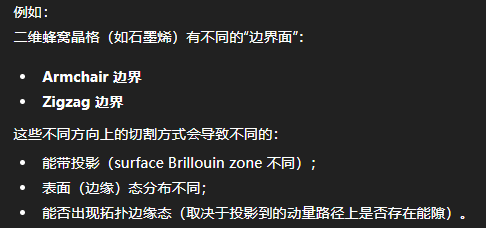
\includegraphics[max width=0.88\linewidth,max height=0.62\textheight,keepaspectratio]{assets/figure-00f3f298596b.png}
\end{figure}\par\par


\par\begin{figure}[H]\centering
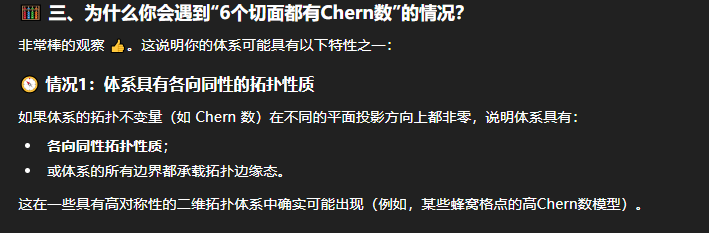
\includegraphics[max width=0.88\linewidth,max height=0.62\textheight,keepaspectratio]{assets/figure-ff1f1a4bcf17.png}
\end{figure}\par\par


\par\begin{figure}[H]\centering
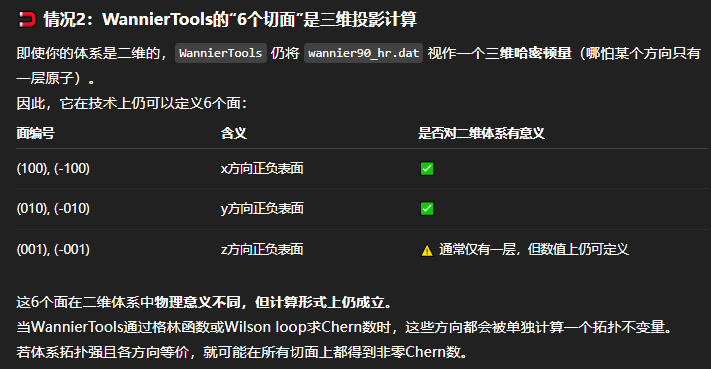
\includegraphics[max width=0.88\linewidth,max height=0.62\textheight,keepaspectratio]{assets/figure-2ab85037124e.png}
\end{figure}\par\par


\par\begin{figure}[H]\centering

\includegraphics[max width=0.88\linewidth,max height=0.62\textheight,keepaspectratio]{assets/figure-67523c0a2b80.png}
\end{figure}\par\par


Q3:实际上vasp对接的是二维体系的能带计算,然后wannier构造wannier函数,但计算的又是三位体系,如何保证计算的物理合理性和数学合理性?\par


A3: 
\par\begin{figure}[H]\centering
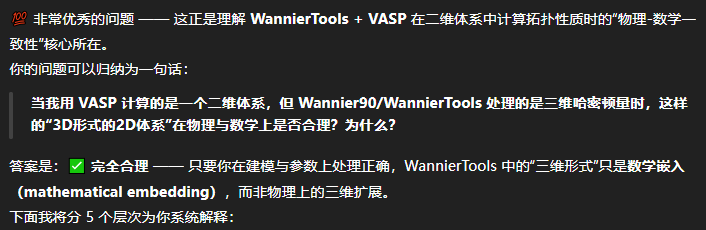
\includegraphics[max width=0.88\linewidth,max height=0.62\textheight,keepaspectratio]{assets/figure-762c34a46c98.png}
\end{figure}\par\par


\par\begin{figure}[H]\centering
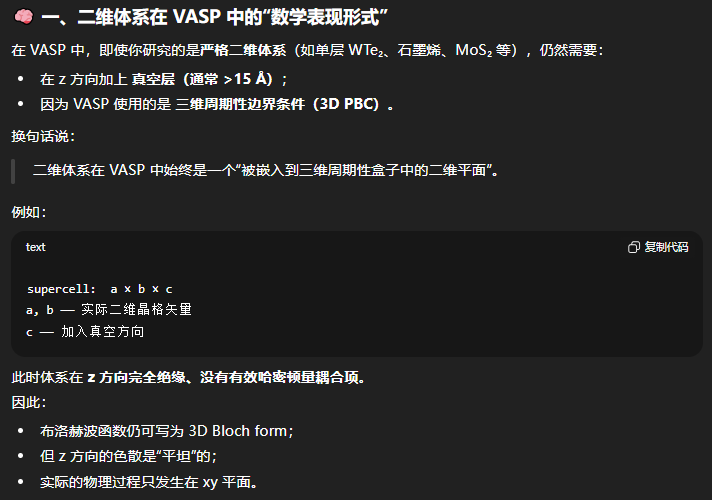
\includegraphics[max width=0.88\linewidth,max height=0.62\textheight,keepaspectratio]{assets/figure-cf15d564a292.png}
\end{figure}\par\par


\par\begin{figure}[H]\centering
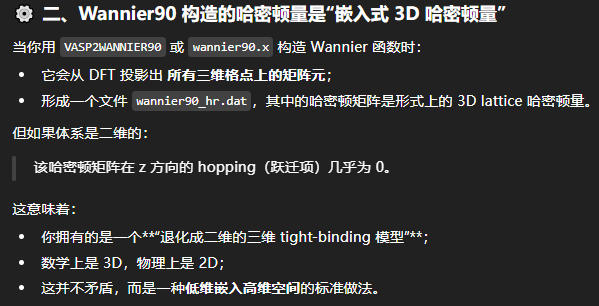
\includegraphics[max width=0.88\linewidth,max height=0.62\textheight,keepaspectratio]{assets/figure-9cf6f3e83501.png}
\end{figure}\par\par


\par\begin{figure}[H]\centering
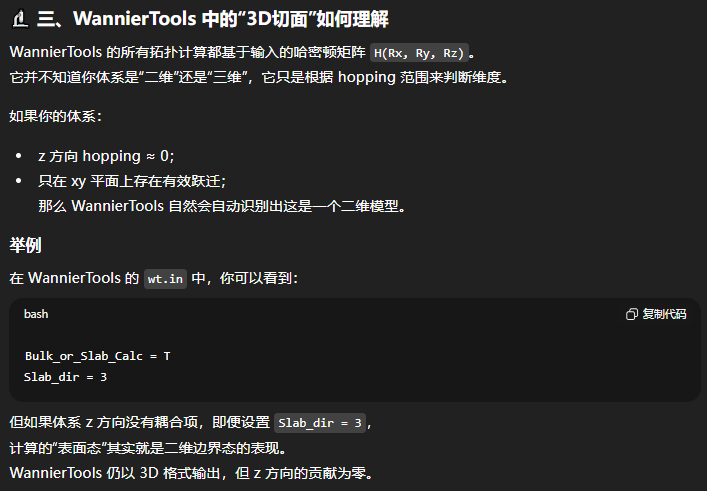
\includegraphics[max width=0.88\linewidth,max height=0.62\textheight,keepaspectratio]{assets/figure-957ea1751eed.png}
\end{figure}\par\par


\par\begin{figure}[H]\centering
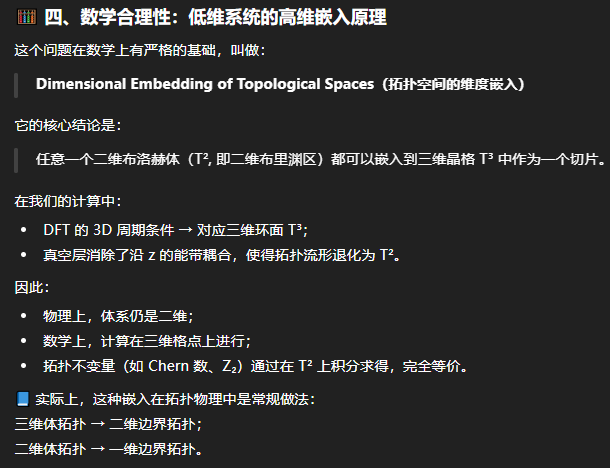
\includegraphics[max width=0.88\linewidth,max height=0.62\textheight,keepaspectratio]{assets/figure-e6cdc9746339.png}
\end{figure}\par\par


Q4: 我看到in文件中的CONTROL中可以选择是否计算bulkband\_\allowbreak{}calc,结合前述结果,似乎一定要计算bulkband?\par


A5: 
\par\begin{figure}[H]\centering
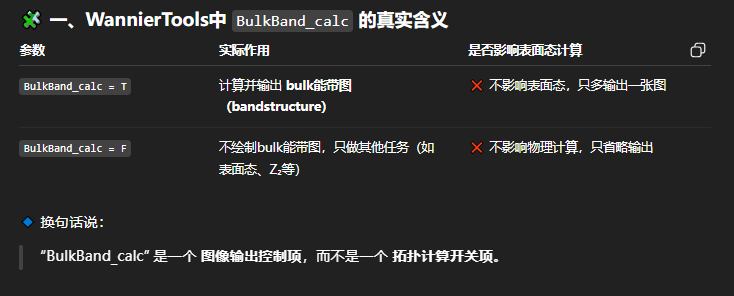
\includegraphics[max width=0.88\linewidth,max height=0.62\textheight,keepaspectratio]{assets/figure-31697f4e9f14.png}
\end{figure}\par\par


\par\begin{figure}[H]\centering
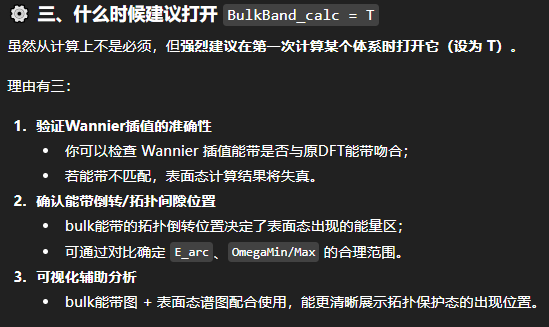
\includegraphics[max width=0.88\linewidth,max height=0.62\textheight,keepaspectratio]{assets/figure-099639f8ab48.png}
\end{figure}\par\par


\par\begin{figure}[H]\centering
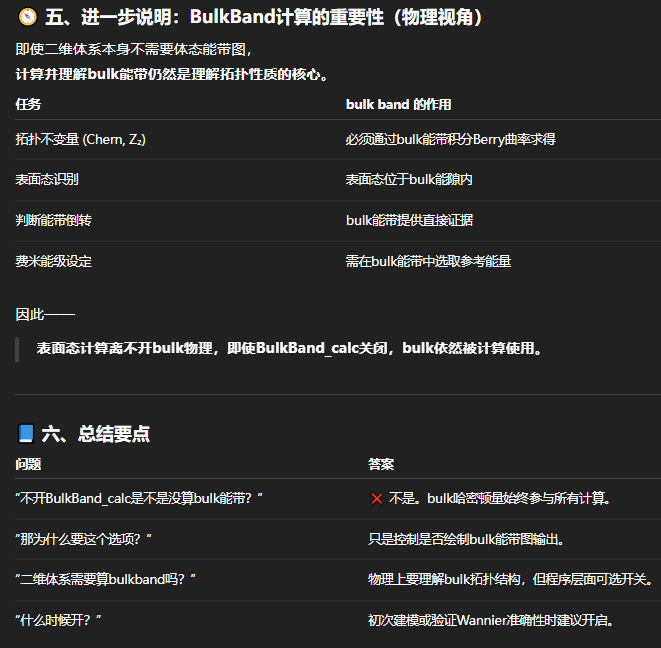
\includegraphics[max width=0.88\linewidth,max height=0.62\textheight,keepaspectratio]{assets/figure-54d4dbb32681.png}
\end{figure}\par\par



\section{pwy90推荐能量窗口测试}
\begin{articlemeta}
\textbf{日期：}2025-11-27\hfill\textbf{在线原文：}\href{https://marx2001.github.io/sci-note\_posts/20251127-pyw1}{marx2001.github.io}
\end{articlemeta}

\subsubsection{心得笔记}


拟合完的指令:wannier90.x wannier90 \& 激活TB2J:source /\allowbreak{}public/\allowbreak{}home/\allowbreak{}cssong/\allowbreak{}song/\allowbreak{}zhchen/\allowbreak{}1\_\allowbreak{}materials/\allowbreak{}1\_\allowbreak{}VTeCl/\allowbreak{}TB2J/\allowbreak{}strain/\allowbreak{}-2/\allowbreak{}TB2J\_\allowbreak{}env/\allowbreak{}bin/\allowbreak{}activate\par


进入pyw90环境:conda activate pyw90\_\allowbreak{}env pyw90 eig suggest –path . -e -20 20 -w 20 在选定能量区间内计算推荐的内外能量窗口的范围\par


求平均值:TB2J\_\allowbreak{}merge.py –type structure x y z\par


求磁耦合参数:wann2J.py –spinor –groupby spin –efermi -1.0098 –emin -2.06514 –emax -0.065 –elements Nb –kmesh 9 9 1 –nz 100 –rcut 6.0 –np 1 第一次测试\par


\subsubsection{测试1}


conda activate pyw90\_\allowbreak{}env\par


pyw90 eig suggest –path . -e -20 20 -w 38\par


\par\begin{figure}[H]\centering
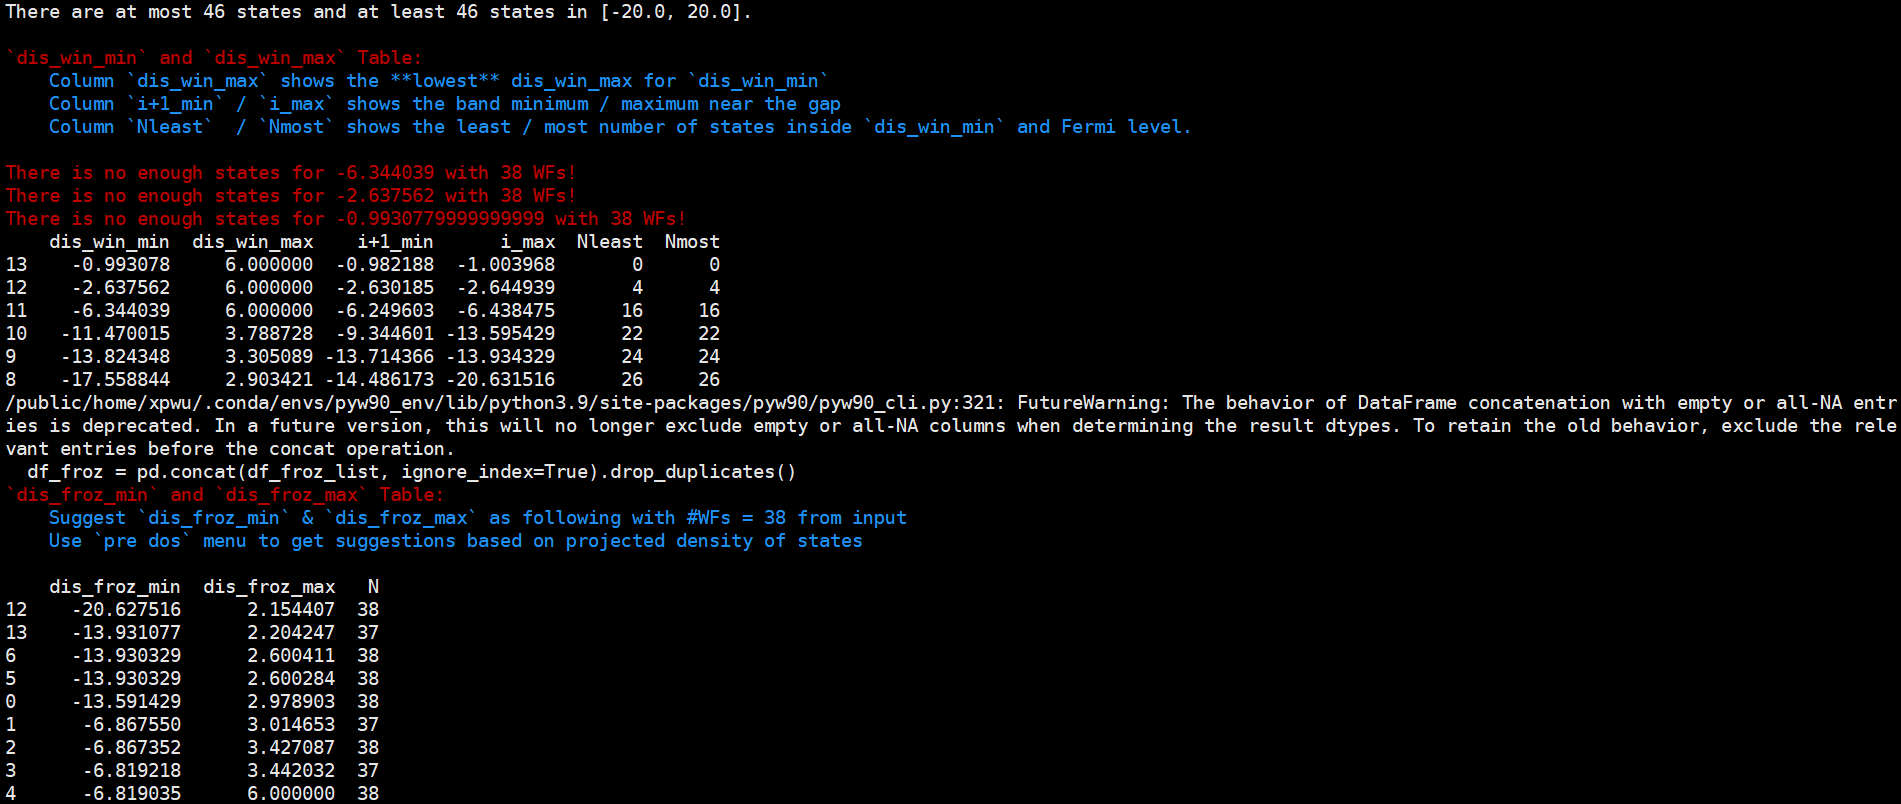
\includegraphics[max width=0.88\linewidth,max height=0.62\textheight,keepaspectratio]{assets/figure-8a1413195a63.png}
\end{figure}\par\par


有个问题,为什么大窗口不满足38个states,而小窗口反而有38个states?\par


\par\begin{figure}[H]\centering
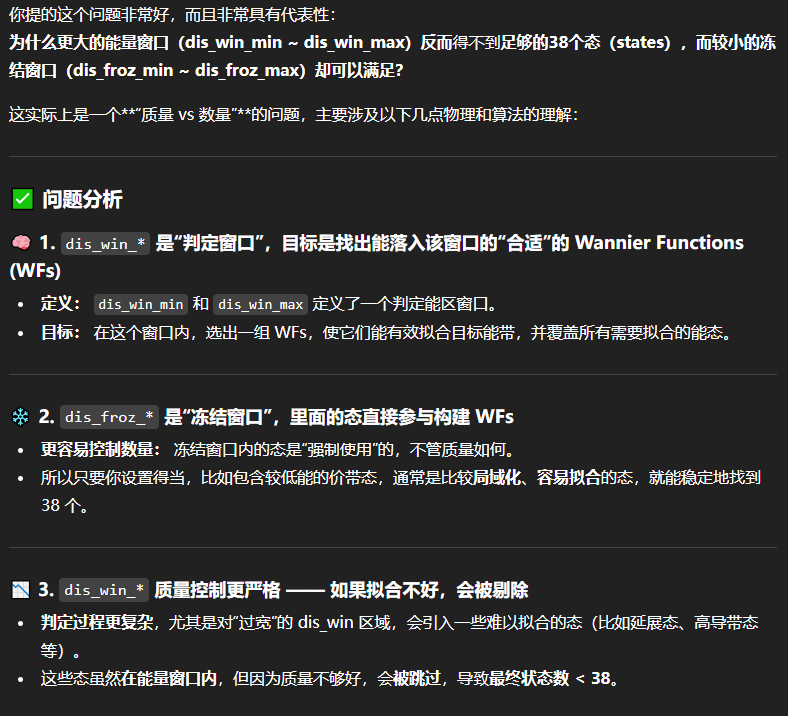
\includegraphics[max width=0.88\linewidth,max height=0.62\textheight,keepaspectratio]{assets/figure-833b6b235e2c.png}
\end{figure}\par\par


\par\begin{figure}[H]\centering
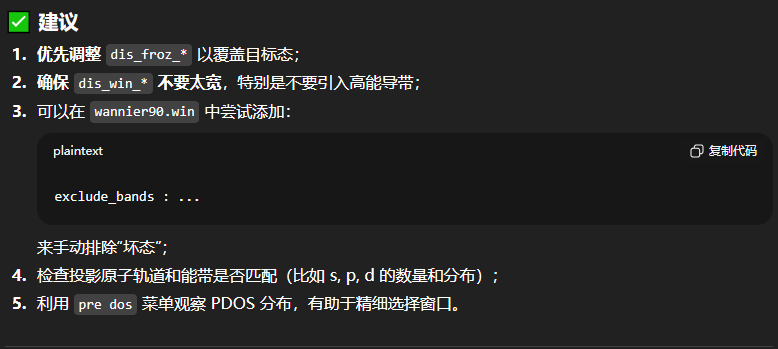
\includegraphics[max width=0.88\linewidth,max height=0.62\textheight,keepaspectratio]{assets/figure-b3072ee3b8e6.png}
\end{figure}\par\par


\par\begin{figure}[H]\centering
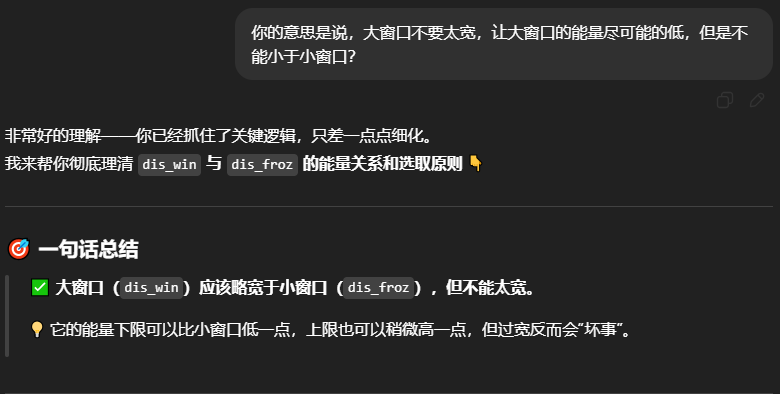
\includegraphics[max width=0.88\linewidth,max height=0.62\textheight,keepaspectratio]{assets/figure-6d31ad2d130f.png}
\end{figure}\par\par


还是有一个问题,这个pyw90判定不足38个态,但是实际上wannier90拟合能带的时候并没有报错,反而拟合的很好,与原来能带完全重合\par


\par\begin{figure}[H]\centering
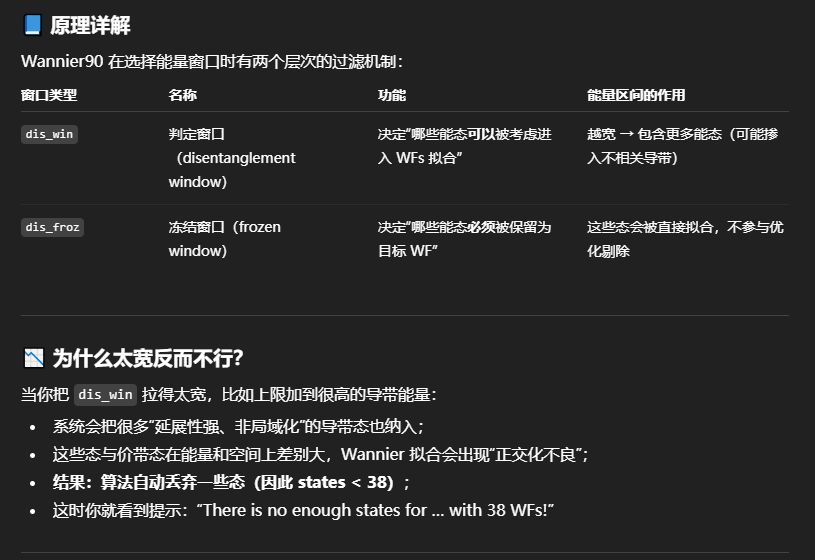
\includegraphics[max width=0.88\linewidth,max height=0.62\textheight,keepaspectratio]{assets/figure-197666d327dd.png}
\end{figure}\par\par


\par\begin{figure}[H]\centering
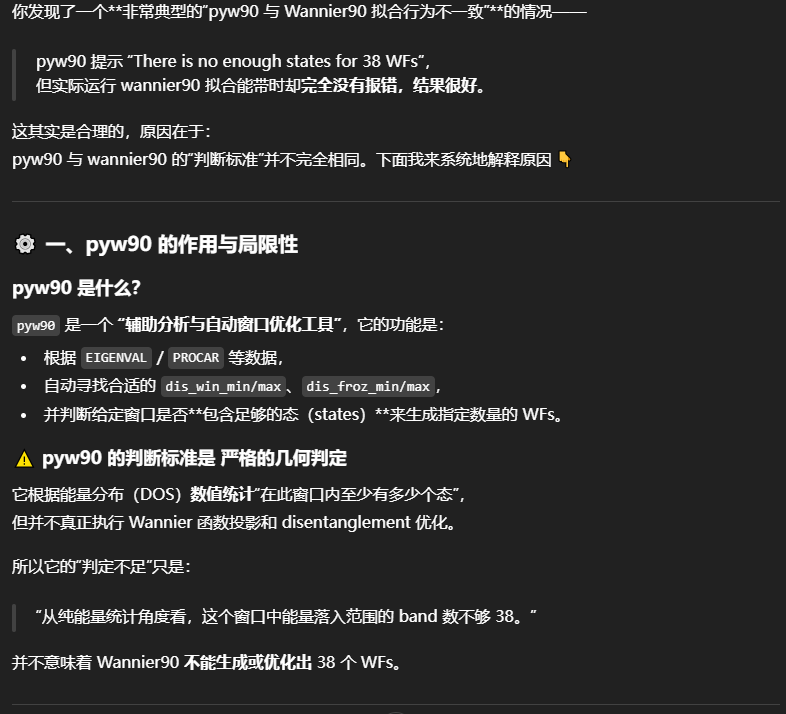
\includegraphics[max width=0.88\linewidth,max height=0.62\textheight,keepaspectratio]{assets/figure-4af6315b4fea.png}
\end{figure}\par\par


\par\begin{figure}[H]\centering
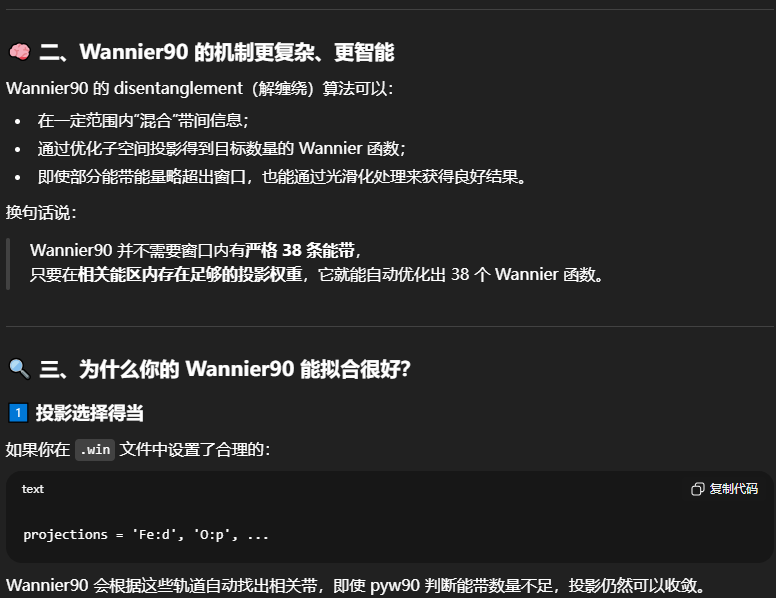
\includegraphics[max width=0.88\linewidth,max height=0.62\textheight,keepaspectratio]{assets/figure-aedd365bbfe0.png}
\end{figure}\par\par


\par\begin{figure}[H]\centering
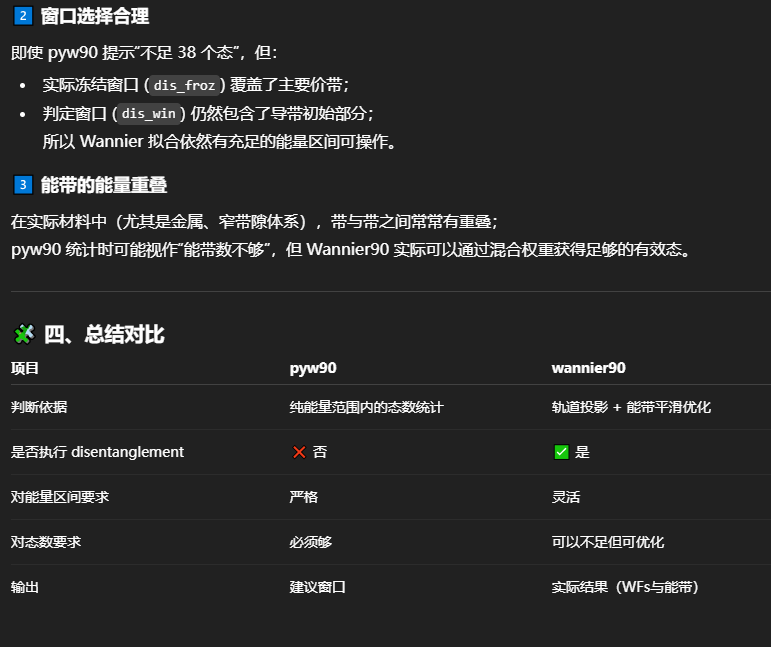
\includegraphics[max width=0.88\linewidth,max height=0.62\textheight,keepaspectratio]{assets/figure-c406328ec990.png}
\end{figure}\par\par


\par\begin{figure}[H]\centering
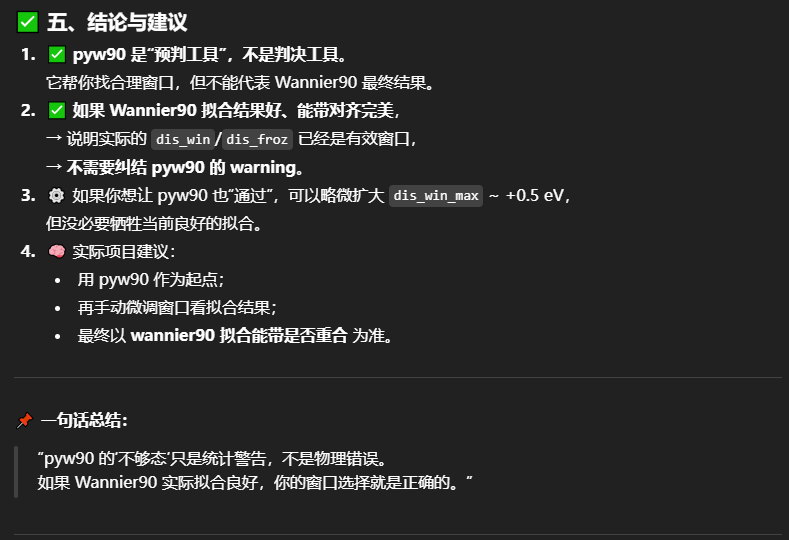
\includegraphics[max width=0.88\linewidth,max height=0.62\textheight,keepaspectratio]{assets/figure-6d12ef68d734.png}
\end{figure}\par\par


与我的已经成功拟合且百分百重合的能带相比,能量窗口的范围,应该是相对靠谱的,可能需要后期手动再调整,可以说能够当作一个预判工具:\par


\par\begin{figure}[H]\centering
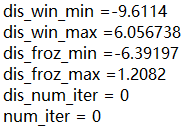
\includegraphics[max width=0.88\linewidth,max height=0.62\textheight,keepaspectratio]{assets/figure-e996c320da30.png}
\end{figure}\par\par


\par\begin{figure}[H]\centering
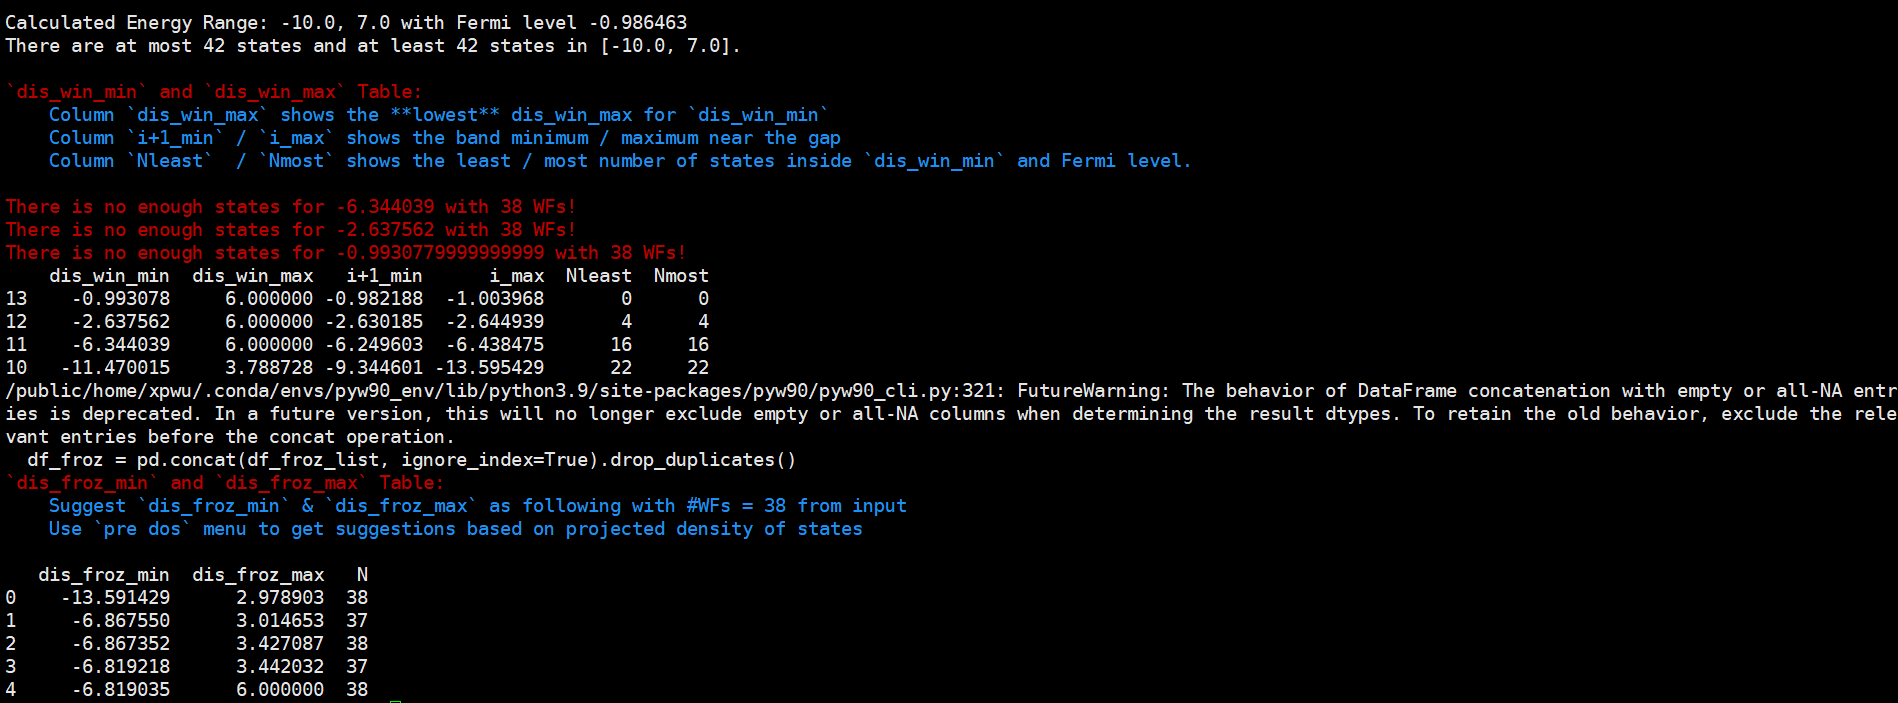
\includegraphics[max width=0.88\linewidth,max height=0.62\textheight,keepaspectratio]{assets/figure-9ecf0ba3756f.png}
\end{figure}\par\par



\section{pyw90的auto功能介绍}
\begin{articlemeta}
\textbf{日期：}2025-11-27\hfill\textbf{在线原文：}\href{https://marx2001.github.io/sci-note\_posts/20251127-pyw-auto}{marx2001.github.io}
\end{articlemeta}

https:/\allowbreak{}/\allowbreak{}github.com/\allowbreak{}Cloudiiink/\allowbreak{}pyw90/\allowbreak{}blob/\allowbreak{}master/\allowbreak{}README.md\par


\subsubsection{简介}


\par\begin{figure}[H]\centering
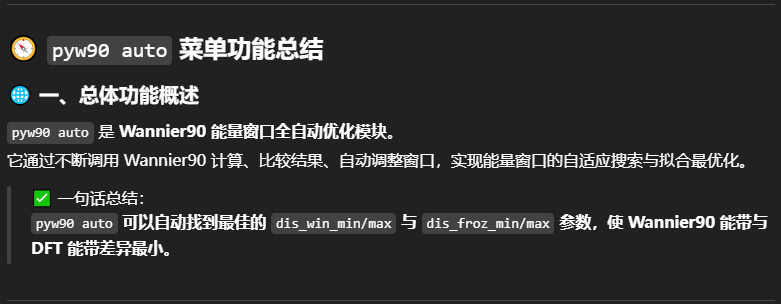
\includegraphics[max width=0.88\linewidth,max height=0.62\textheight,keepaspectratio]{assets/figure-f5a1c884ad37.png}
\end{figure}\par\par


\par\begin{figure}[H]\centering
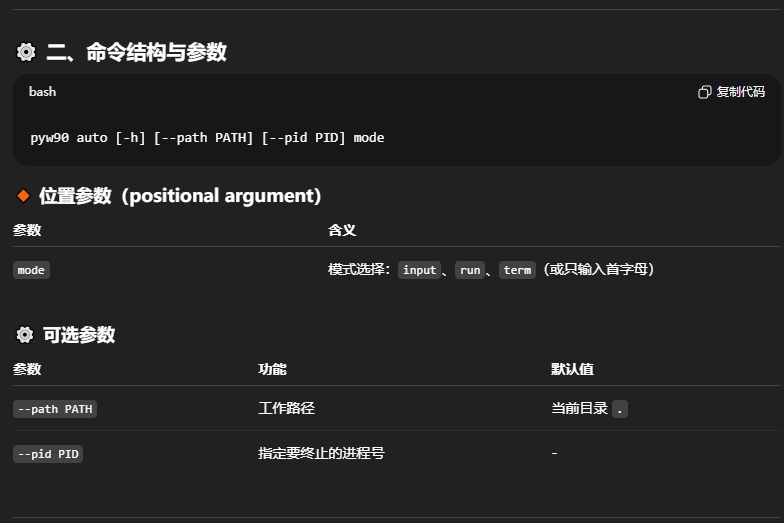
\includegraphics[max width=0.88\linewidth,max height=0.62\textheight,keepaspectratio]{assets/figure-94535843b624.png}
\end{figure}\par\par


\par\begin{figure}[H]\centering
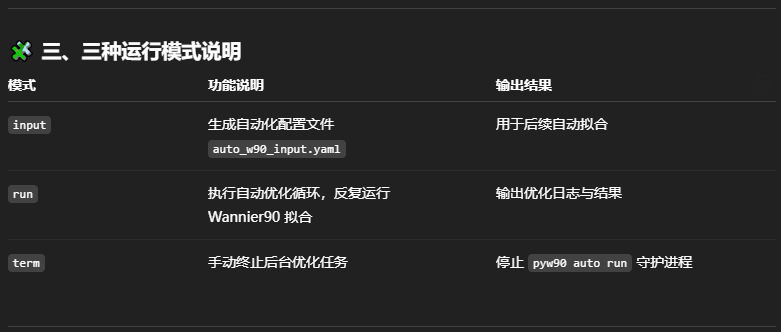
\includegraphics[max width=0.88\linewidth,max height=0.62\textheight,keepaspectratio]{assets/figure-cc59b284395c.png}
\end{figure}\par\par


\par\begin{figure}[H]\centering
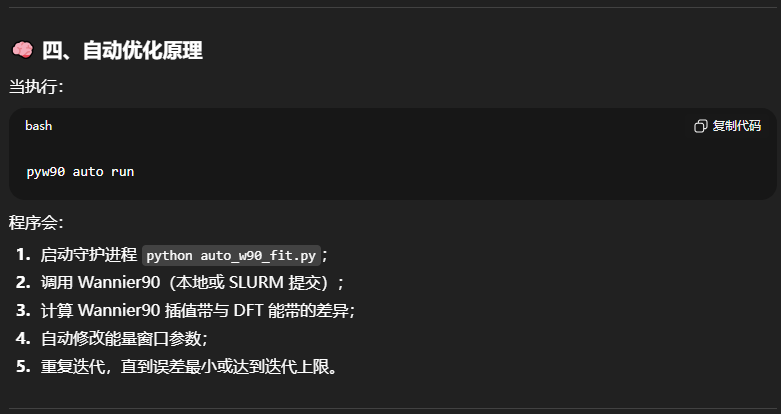
\includegraphics[max width=0.88\linewidth,max height=0.62\textheight,keepaspectratio]{assets/figure-8fcd59f0f7c9.png}
\end{figure}\par\par


\par\begin{figure}[H]\centering
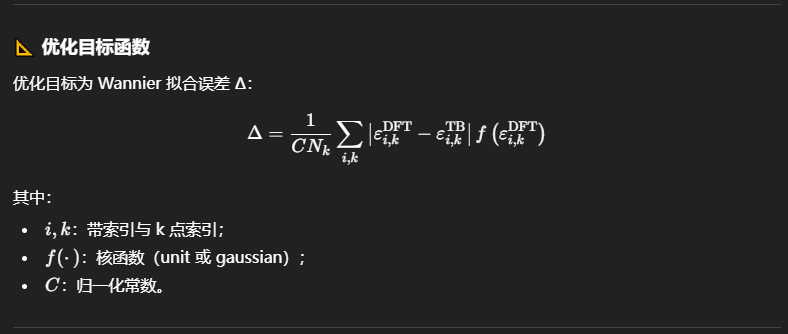
\includegraphics[max width=0.88\linewidth,max height=0.62\textheight,keepaspectratio]{assets/figure-dc0ff9634ab0.png}
\end{figure}\par\par


\par\begin{figure}[H]\centering

\includegraphics[max width=0.88\linewidth,max height=0.62\textheight,keepaspectratio]{assets/figure-9742037530e1.png}
\end{figure}\par\par


\par\begin{figure}[H]\centering
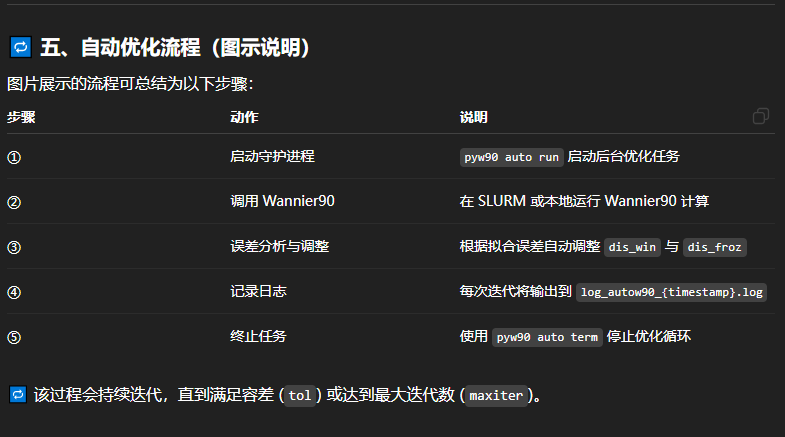
\includegraphics[max width=0.88\linewidth,max height=0.62\textheight,keepaspectratio]{assets/figure-d05a793b81a6.png}
\end{figure}\par\par


\par\begin{figure}[H]\centering
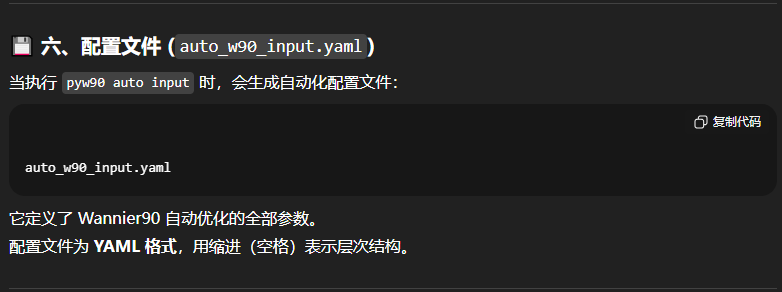
\includegraphics[max width=0.88\linewidth,max height=0.62\textheight,keepaspectratio]{assets/figure-c94f587a8e66.png}
\end{figure}\par\par


\par\begin{figure}[H]\centering
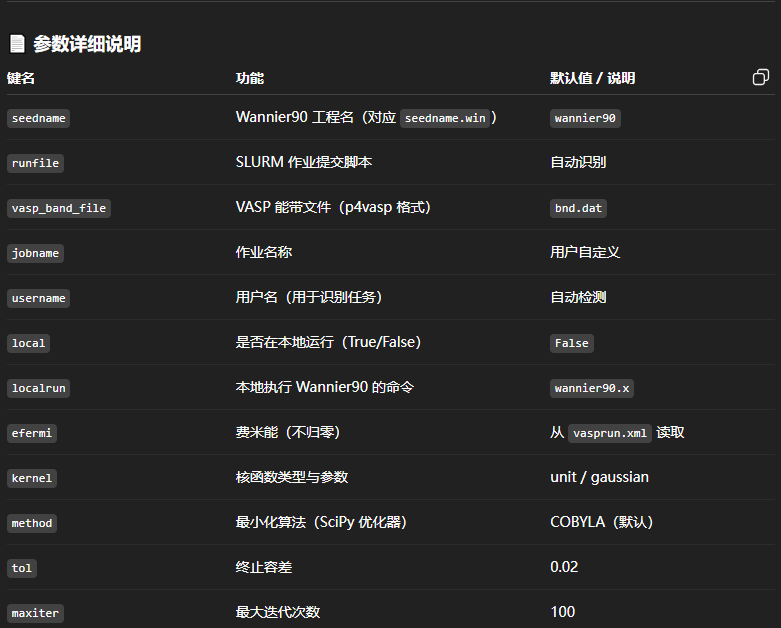
\includegraphics[max width=0.88\linewidth,max height=0.62\textheight,keepaspectratio]{assets/figure-f135d7de0a02.png}
\end{figure}\par\par


\par\begin{figure}[H]\centering
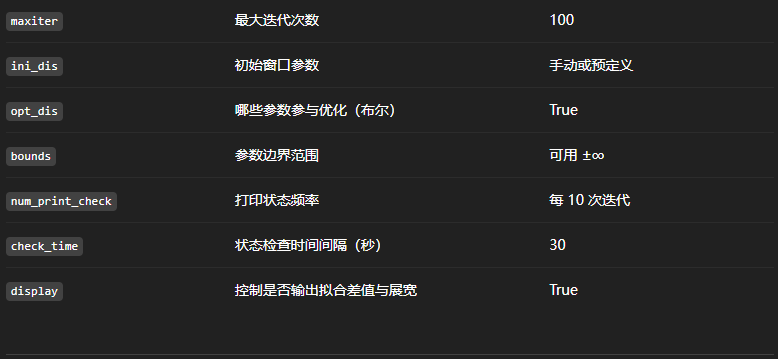
\includegraphics[max width=0.88\linewidth,max height=0.62\textheight,keepaspectratio]{assets/figure-b6a424f0c0a2.png}
\end{figure}\par\par


\par\begin{figure}[H]\centering
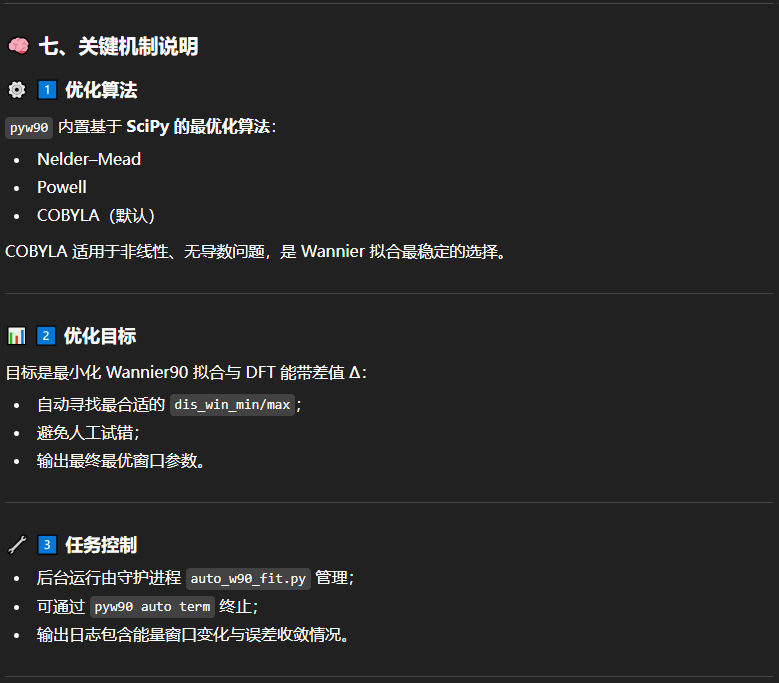
\includegraphics[max width=0.88\linewidth,max height=0.62\textheight,keepaspectratio]{assets/figure-942ae03fefcc.png}
\end{figure}\par\par


\par\begin{figure}[H]\centering
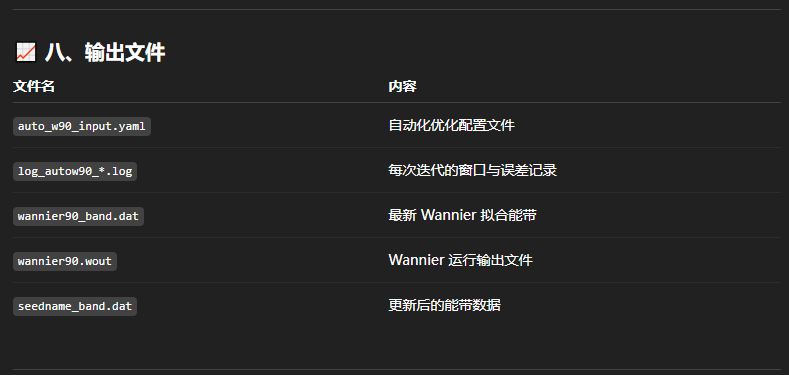
\includegraphics[max width=0.88\linewidth,max height=0.62\textheight,keepaspectratio]{assets/figure-86c7f2a6f0a1.png}
\end{figure}\par\par


\par\begin{figure}[H]\centering
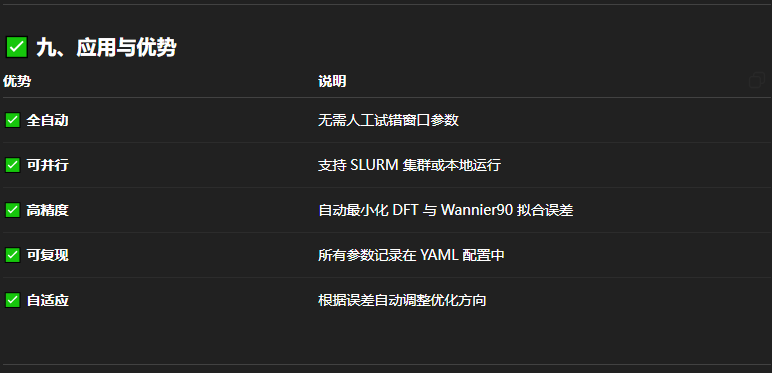
\includegraphics[max width=0.88\linewidth,max height=0.62\textheight,keepaspectratio]{assets/figure-0bee1b2fe5fa.png}
\end{figure}\par\par


\par\begin{figure}[H]\centering
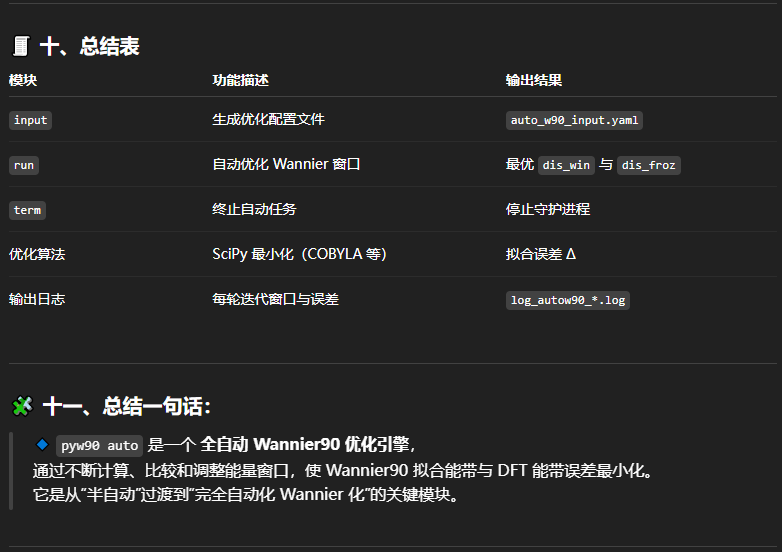
\includegraphics[max width=0.88\linewidth,max height=0.62\textheight,keepaspectratio]{assets/figure-eb5cf8c1688a.png}
\end{figure}\par\par


Q1:wannier90的能带拟合步骤是通过设置VASP中的INCAR中的LWANNIER90=.T的tag实现的,在此过程中,vasp先计算能带,然后通过上面那个接口输出为wannier格式,那么这个pyw90是怎么确定拟合出来的结果和窗口能量区间是正确的呢?\par


A1:\par


\par\begin{figure}[H]\centering
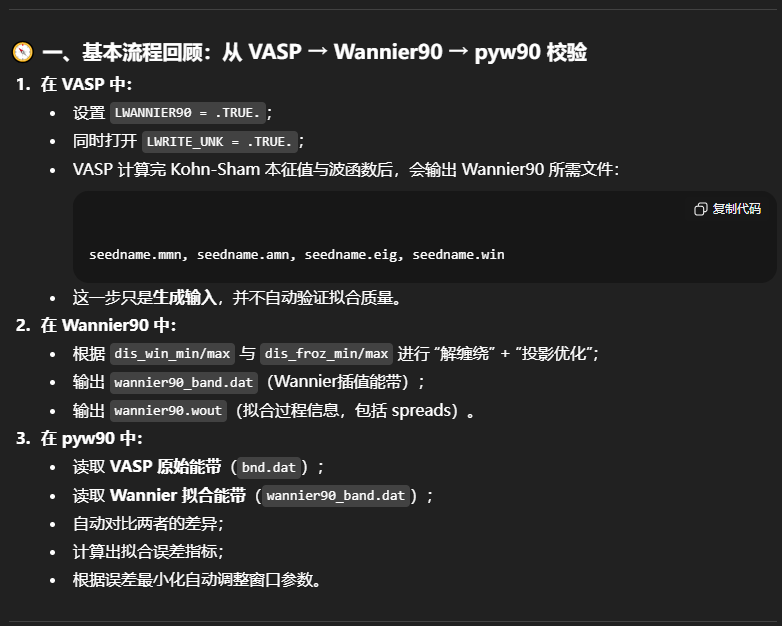
\includegraphics[max width=0.88\linewidth,max height=0.62\textheight,keepaspectratio]{assets/figure-75a2e85177d8.png}
\end{figure}\par\par


\par\begin{figure}[H]\centering
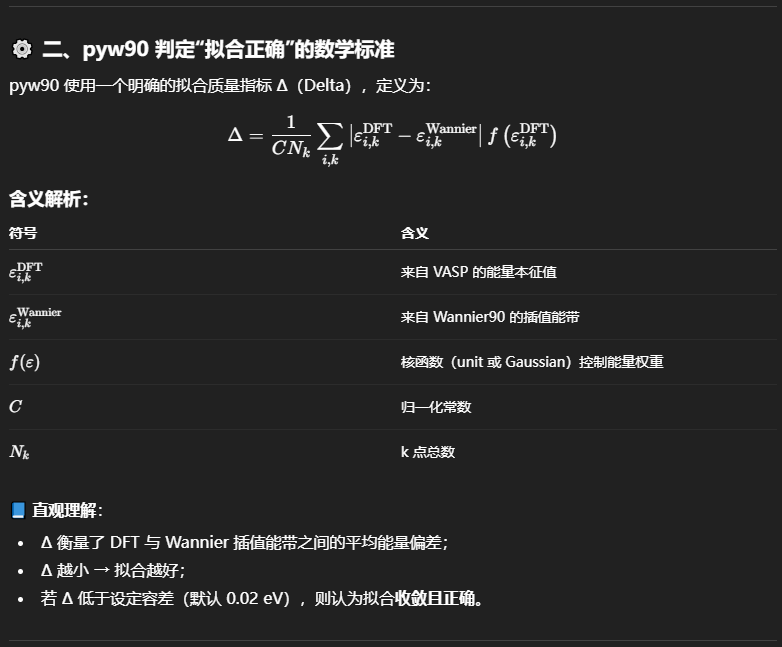
\includegraphics[max width=0.88\linewidth,max height=0.62\textheight,keepaspectratio]{assets/figure-040f9ad8c169.png}
\end{figure}\par\par


\par\begin{figure}[H]\centering
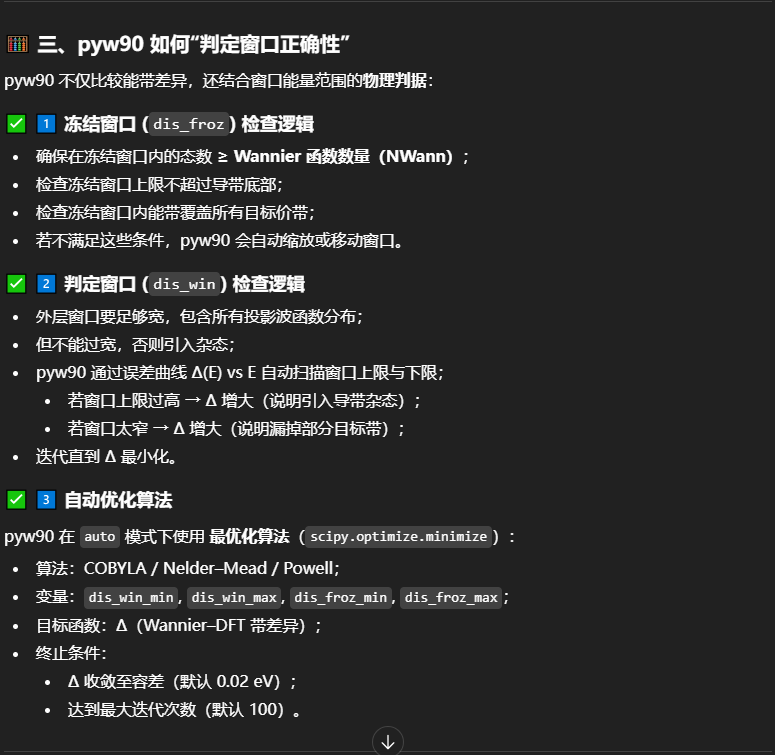
\includegraphics[max width=0.88\linewidth,max height=0.62\textheight,keepaspectratio]{assets/figure-f0dfc014fa6f.png}
\end{figure}\par\par


\par\begin{figure}[H]\centering
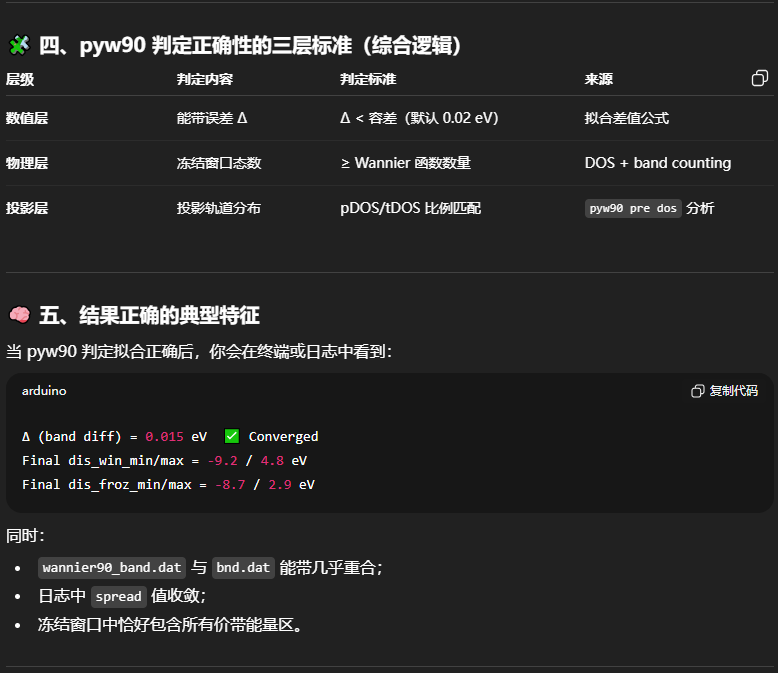
\includegraphics[max width=0.88\linewidth,max height=0.62\textheight,keepaspectratio]{assets/figure-3ca694b9f06c.png}
\end{figure}\par\par


\par\begin{figure}[H]\centering
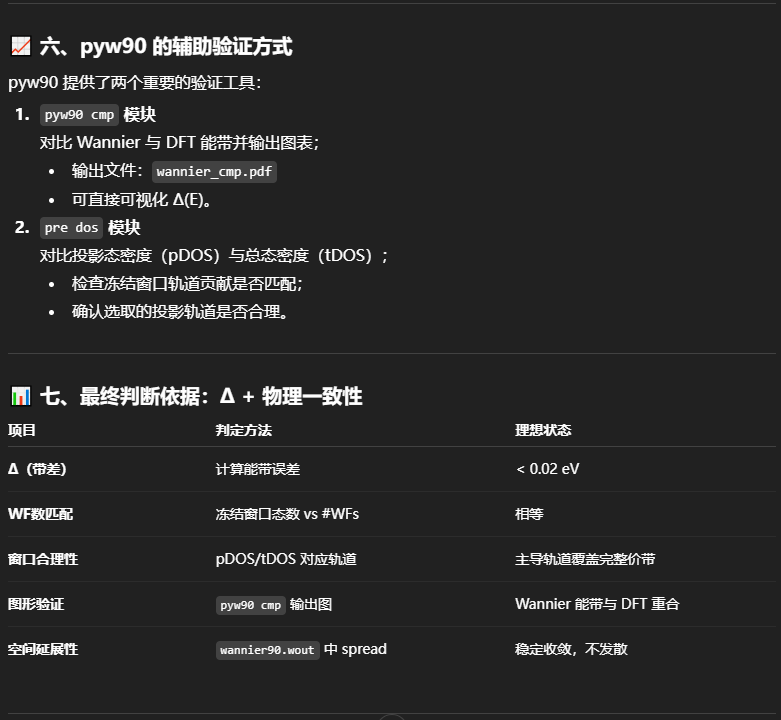
\includegraphics[max width=0.88\linewidth,max height=0.62\textheight,keepaspectratio]{assets/figure-99cc04a3c6a4.png}
\end{figure}\par\par


\par\begin{figure}[H]\centering
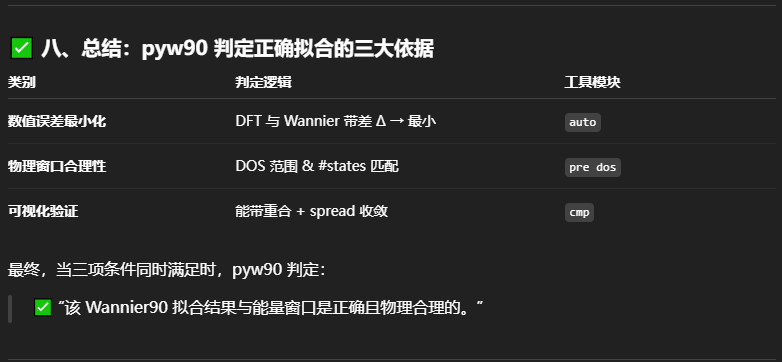
\includegraphics[max width=0.88\linewidth,max height=0.62\textheight,keepaspectratio]{assets/figure-2805648d0e9e.png}
\end{figure}\par\par



\section{pyw90的cmp功能介绍}
\begin{articlemeta}
\textbf{日期：}2025-11-27\hfill\textbf{在线原文：}\href{https://marx2001.github.io/sci-note\_posts/20251127-pyw-cmap}{marx2001.github.io}
\end{articlemeta}

https:/\allowbreak{}/\allowbreak{}github.com/\allowbreak{}Cloudiiink/\allowbreak{}pyw90/\allowbreak{}blob/\allowbreak{}master/\allowbreak{}README.md\par


\subsubsection{简介}


\par\begin{figure}[H]\centering
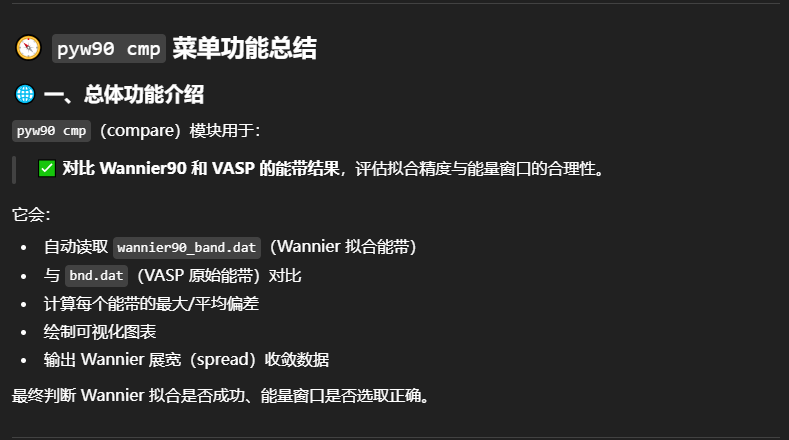
\includegraphics[max width=0.88\linewidth,max height=0.62\textheight,keepaspectratio]{assets/figure-4c4ce1047d57.png}
\end{figure}\par\par


\par\begin{figure}[H]\centering
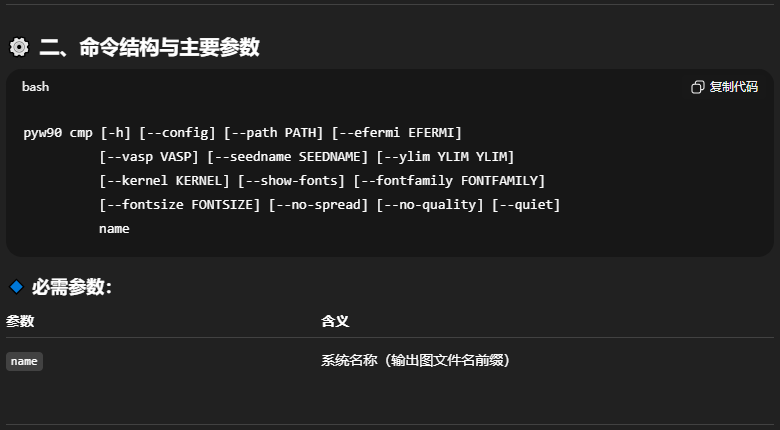
\includegraphics[max width=0.88\linewidth,max height=0.62\textheight,keepaspectratio]{assets/figure-3ef6ae16c153.png}
\end{figure}\par\par


\par\begin{figure}[H]\centering
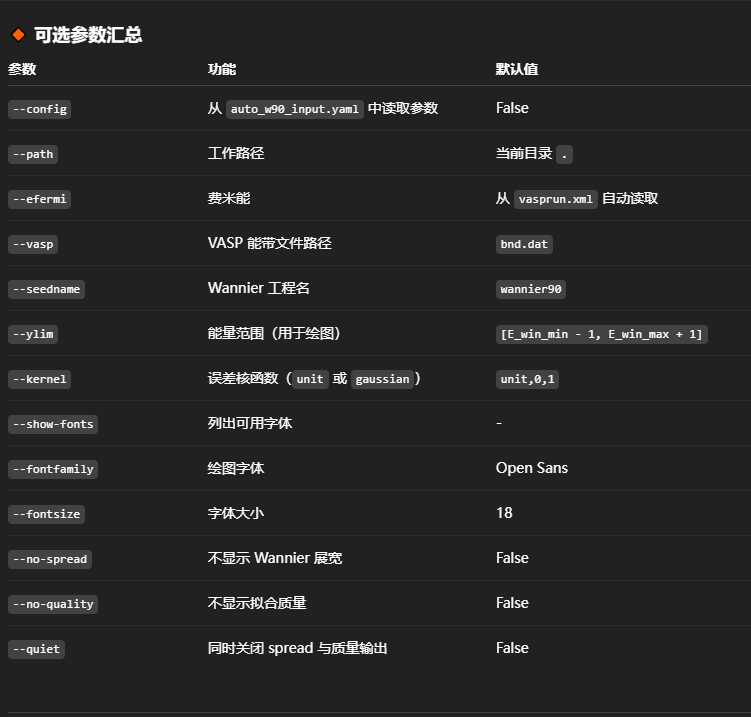
\includegraphics[max width=0.88\linewidth,max height=0.62\textheight,keepaspectratio]{assets/figure-0dc1932a6467.png}
\end{figure}\par\par


\par\begin{figure}[H]\centering
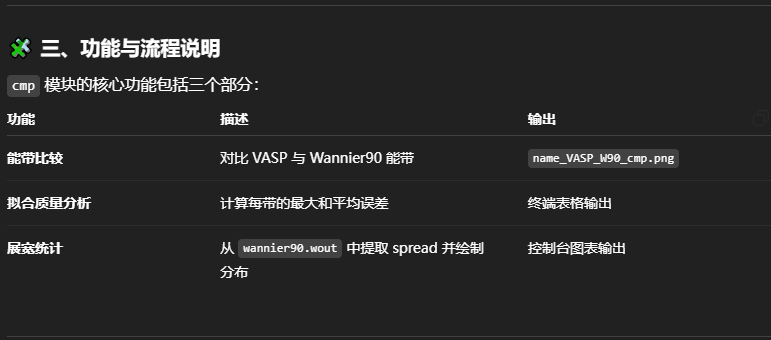
\includegraphics[max width=0.88\linewidth,max height=0.62\textheight,keepaspectratio]{assets/figure-bf2c2f74e318.png}
\end{figure}\par\par


\par\begin{figure}[H]\centering
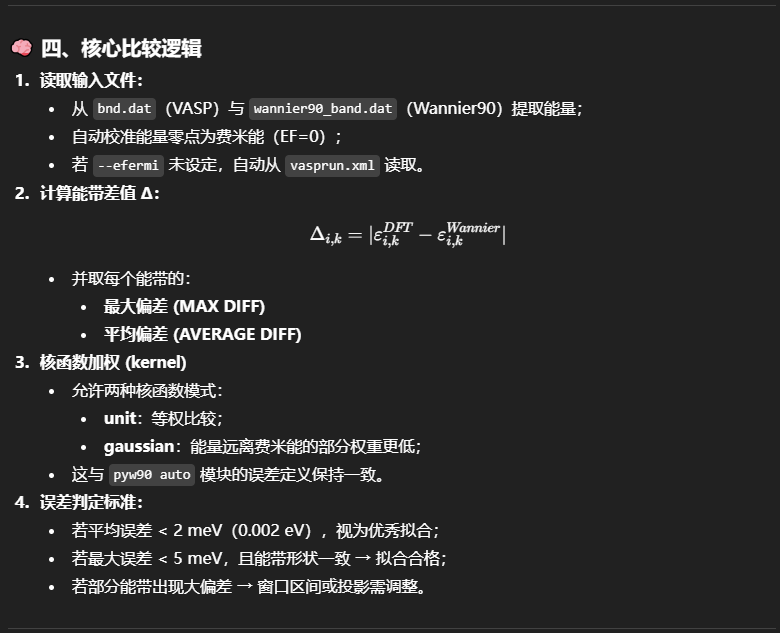
\includegraphics[max width=0.88\linewidth,max height=0.62\textheight,keepaspectratio]{assets/figure-6a184886b69b.png}
\end{figure}\par\par


\par\begin{figure}[H]\centering
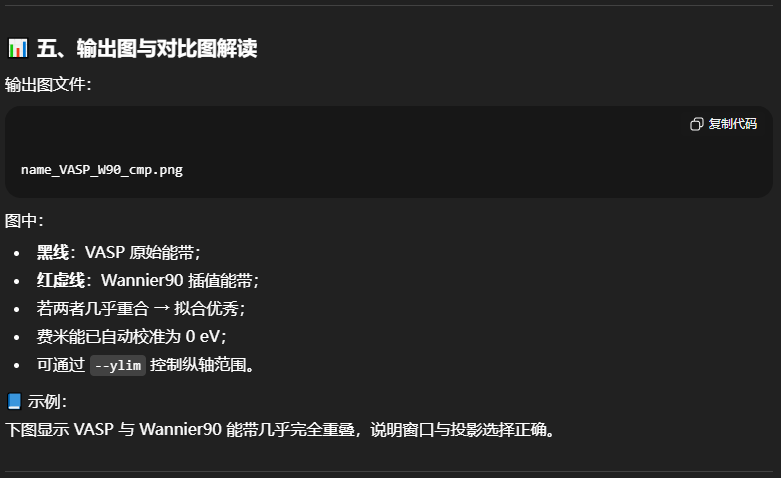
\includegraphics[max width=0.88\linewidth,max height=0.62\textheight,keepaspectratio]{assets/figure-a3ab59ad59b6.png}
\end{figure}\par\par


\par\begin{figure}[H]\centering
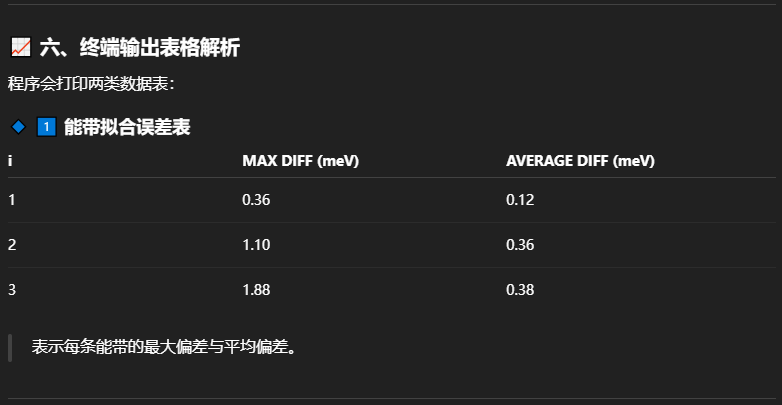
\includegraphics[max width=0.88\linewidth,max height=0.62\textheight,keepaspectratio]{assets/figure-8fab92b83634.png}
\end{figure}\par\par


\par\begin{figure}[H]\centering
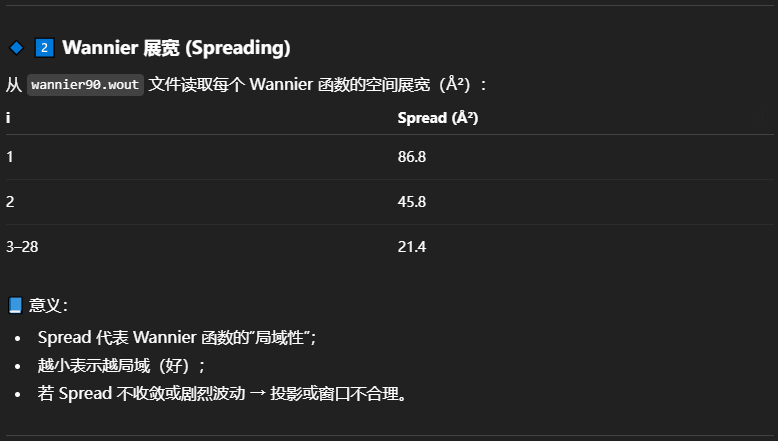
\includegraphics[max width=0.88\linewidth,max height=0.62\textheight,keepaspectratio]{assets/figure-378fbc103626.png}
\end{figure}\par\par


\par\begin{figure}[H]\centering
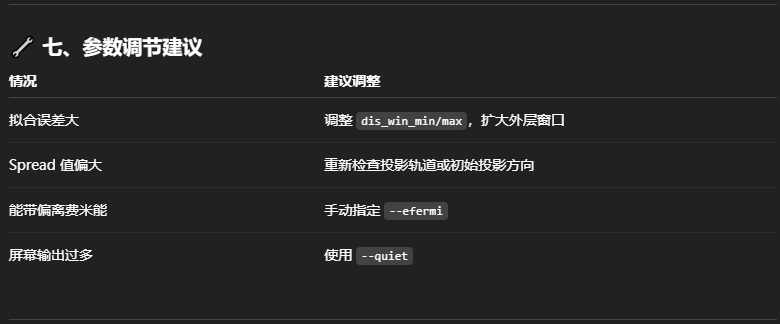
\includegraphics[max width=0.88\linewidth,max height=0.62\textheight,keepaspectratio]{assets/figure-41a9518760f1.png}
\end{figure}\par\par


\par\begin{figure}[H]\centering
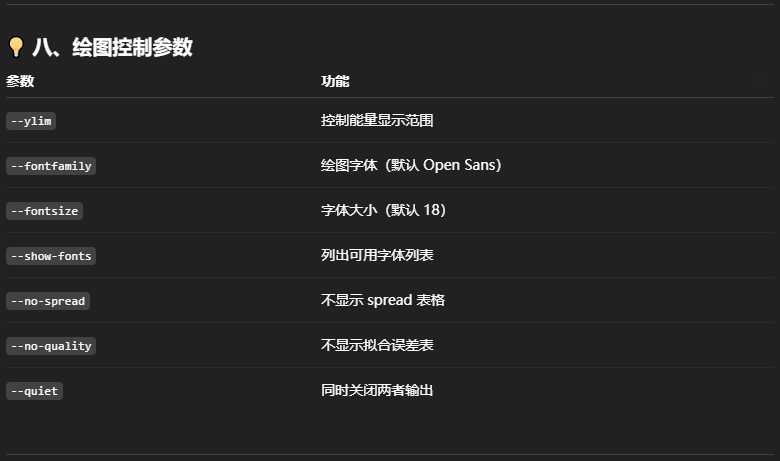
\includegraphics[max width=0.88\linewidth,max height=0.62\textheight,keepaspectratio]{assets/figure-6a8519f15978.png}
\end{figure}\par\par


\par\begin{figure}[H]\centering
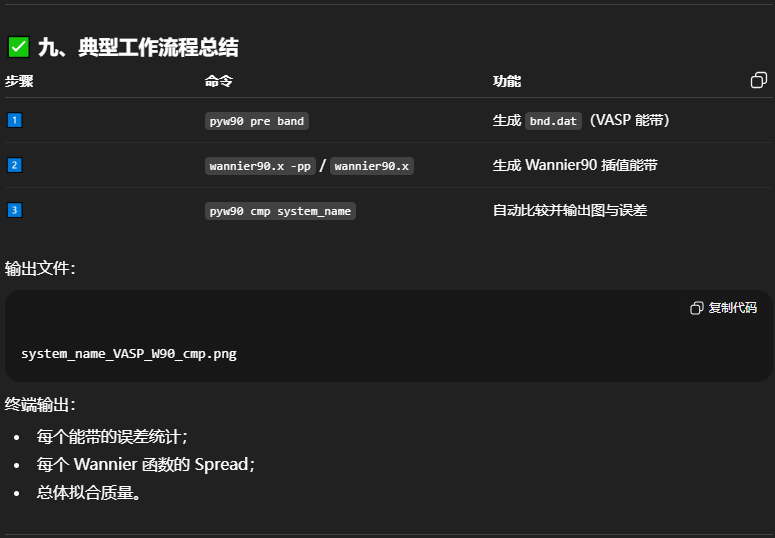
\includegraphics[max width=0.88\linewidth,max height=0.62\textheight,keepaspectratio]{assets/figure-9df36ed23969.png}
\end{figure}\par\par


\par\begin{figure}[H]\centering
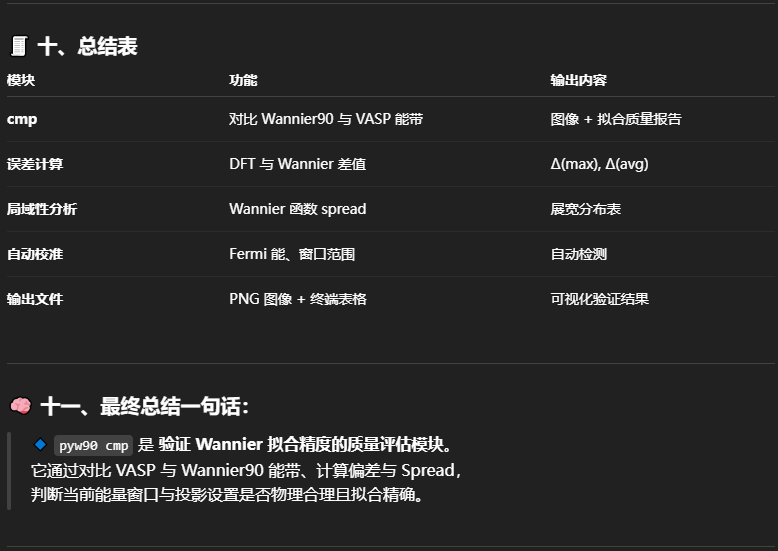
\includegraphics[max width=0.88\linewidth,max height=0.62\textheight,keepaspectratio]{assets/figure-e8391e83fea9.png}
\end{figure}\par\par



\section{pyw90的eig功能介绍}
\begin{articlemeta}
\textbf{日期：}2025-11-27\hfill\textbf{在线原文：}\href{https://marx2001.github.io/sci-note\_posts/20251127-pyw-eig}{marx2001.github.io}
\end{articlemeta}

https:/\allowbreak{}/\allowbreak{}github.com/\allowbreak{}Cloudiiink/\allowbreak{}pyw90/\allowbreak{}blob/\allowbreak{}master/\allowbreak{}README.md\par


\subsubsection{简介}


\par\begin{figure}[H]\centering
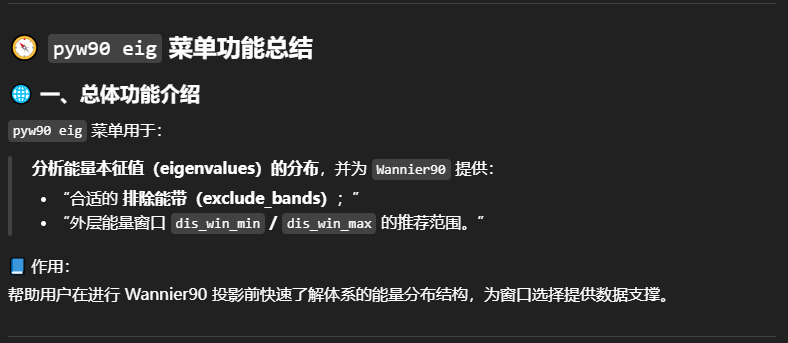
\includegraphics[max width=0.88\linewidth,max height=0.62\textheight,keepaspectratio]{assets/figure-505e282645e1.png}
\end{figure}\par\par


\par\begin{figure}[H]\centering
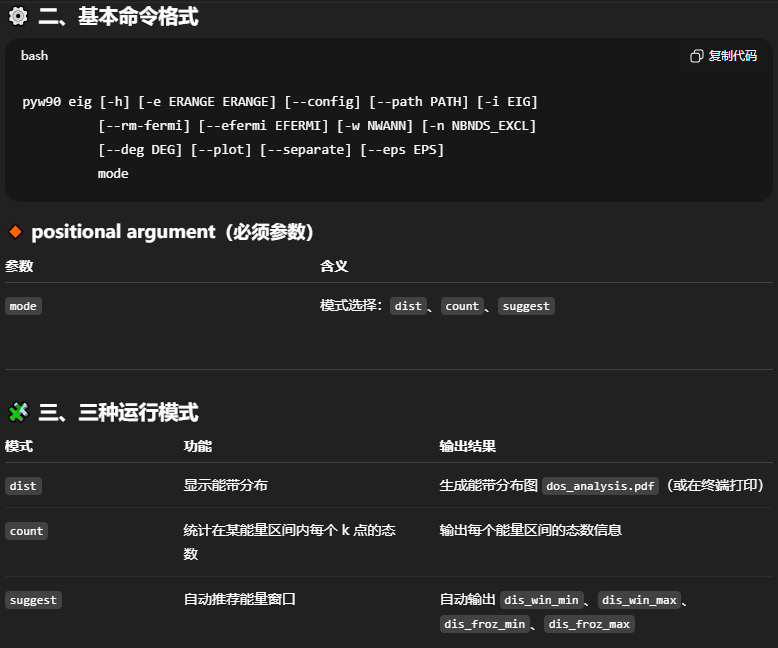
\includegraphics[max width=0.88\linewidth,max height=0.62\textheight,keepaspectratio]{assets/figure-ddf22d1ba32d.png}
\end{figure}\par\par


\par\begin{figure}[H]\centering
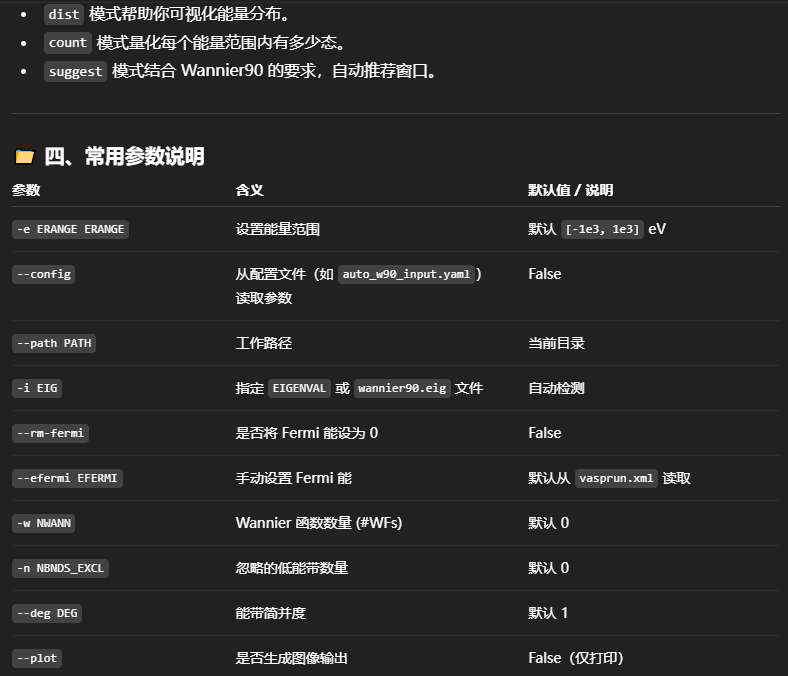
\includegraphics[max width=0.88\linewidth,max height=0.62\textheight,keepaspectratio]{assets/figure-829308c67948.png}
\end{figure}\par\par


\par\begin{figure}[H]\centering
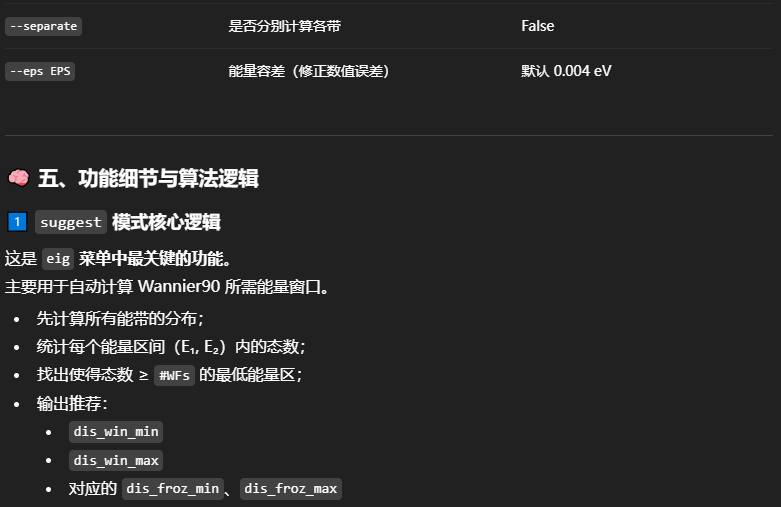
\includegraphics[max width=0.88\linewidth,max height=0.62\textheight,keepaspectratio]{assets/figure-e30f3a5dc645.png}
\end{figure}\par\par


\par\begin{figure}[H]\centering
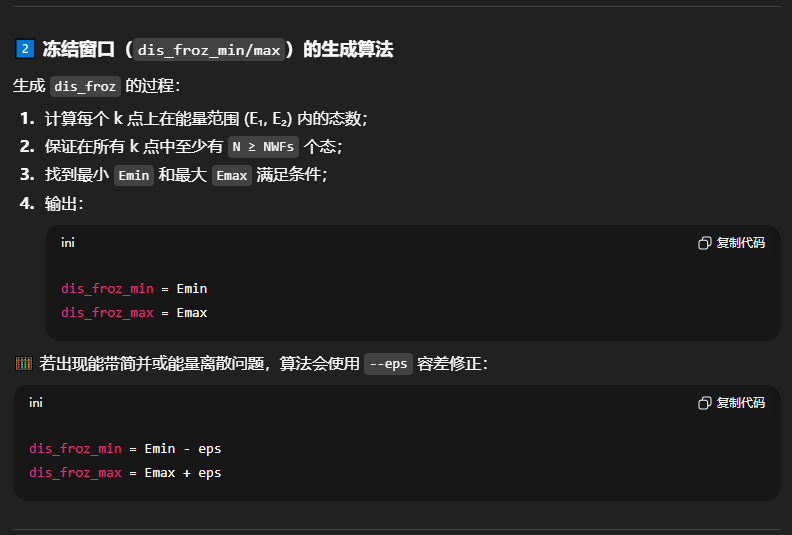
\includegraphics[max width=0.88\linewidth,max height=0.62\textheight,keepaspectratio]{assets/figure-61f75fc72898.png}
\end{figure}\par\par


\par\begin{figure}[H]\centering
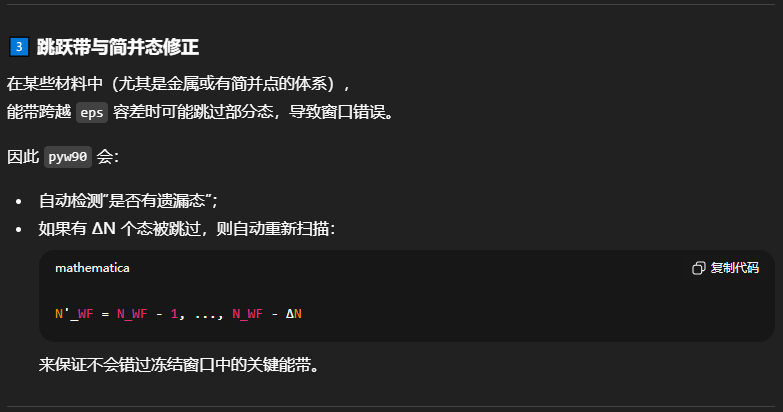
\includegraphics[max width=0.88\linewidth,max height=0.62\textheight,keepaspectratio]{assets/figure-756bc1bc3471.png}
\end{figure}\par\par


\par\begin{figure}[H]\centering
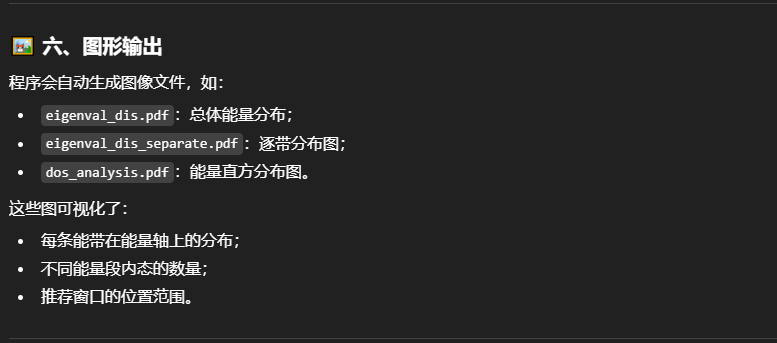
\includegraphics[max width=0.88\linewidth,max height=0.62\textheight,keepaspectratio]{assets/figure-d2e1cb288278.png}
\end{figure}\par\par


\par\begin{figure}[H]\centering
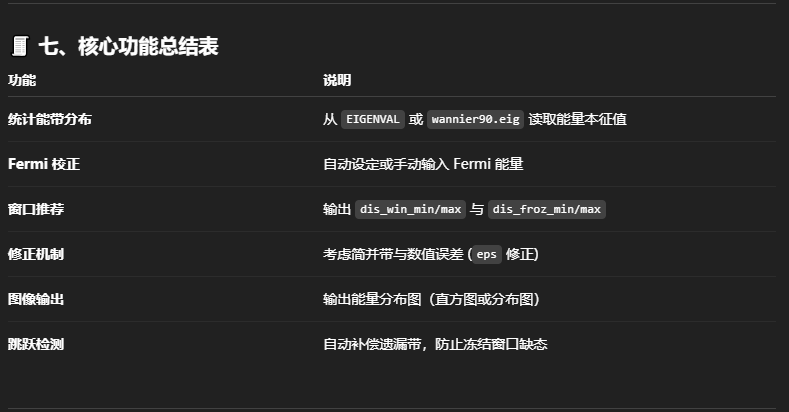
\includegraphics[max width=0.88\linewidth,max height=0.62\textheight,keepaspectratio]{assets/figure-94672265a967.png}
\end{figure}\par\par


\par\begin{figure}[H]\centering
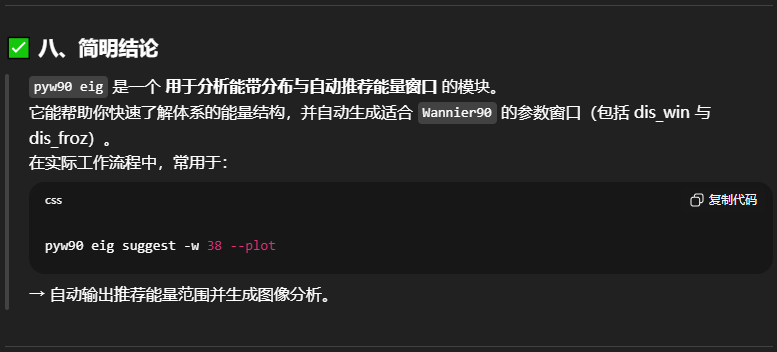
\includegraphics[max width=0.88\linewidth,max height=0.62\textheight,keepaspectratio]{assets/figure-92a65ce27137.png}
\end{figure}\par\par



\section{pyw90的pre功能介绍}
\begin{articlemeta}
\textbf{日期：}2025-11-27\hfill\textbf{在线原文：}\href{https://marx2001.github.io/sci-note\_posts/20251127-pyw-pre}{marx2001.github.io}
\end{articlemeta}

https:/\allowbreak{}/\allowbreak{}github.com/\allowbreak{}Cloudiiink/\allowbreak{}pyw90/\allowbreak{}blob/\allowbreak{}master/\allowbreak{}README.md\par


\subsubsection{简介}


\par\begin{figure}[H]\centering
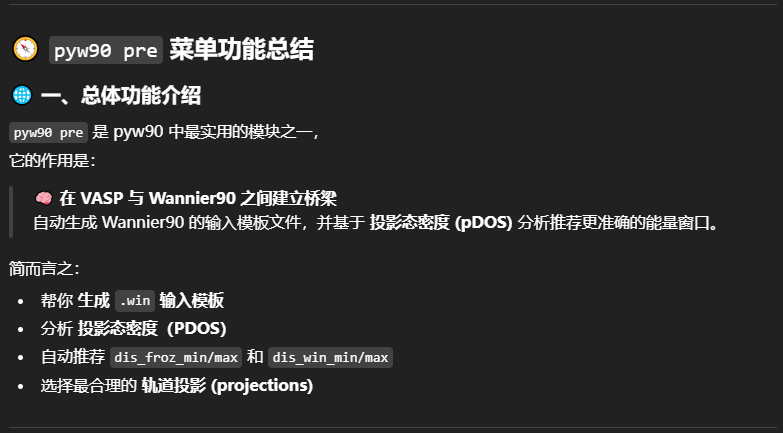
\includegraphics[max width=0.88\linewidth,max height=0.62\textheight,keepaspectratio]{assets/figure-0f75fa2c4d13.png}
\end{figure}\par\par


\par\begin{figure}[H]\centering
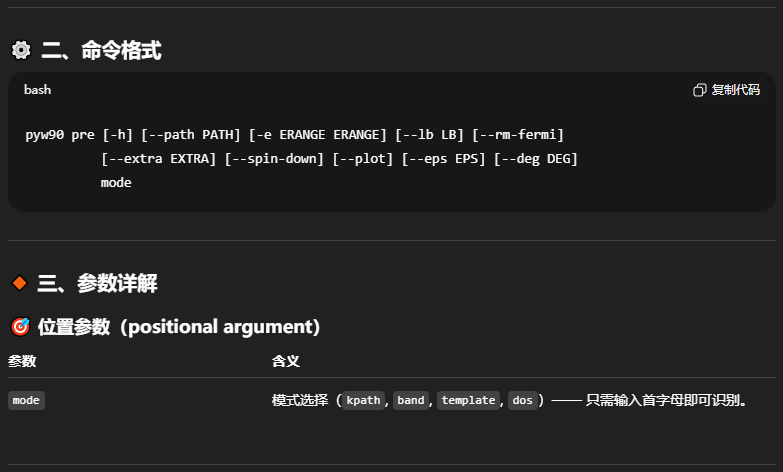
\includegraphics[max width=0.88\linewidth,max height=0.62\textheight,keepaspectratio]{assets/figure-22ccf816b504.png}
\end{figure}\par\par


\par\begin{figure}[H]\centering
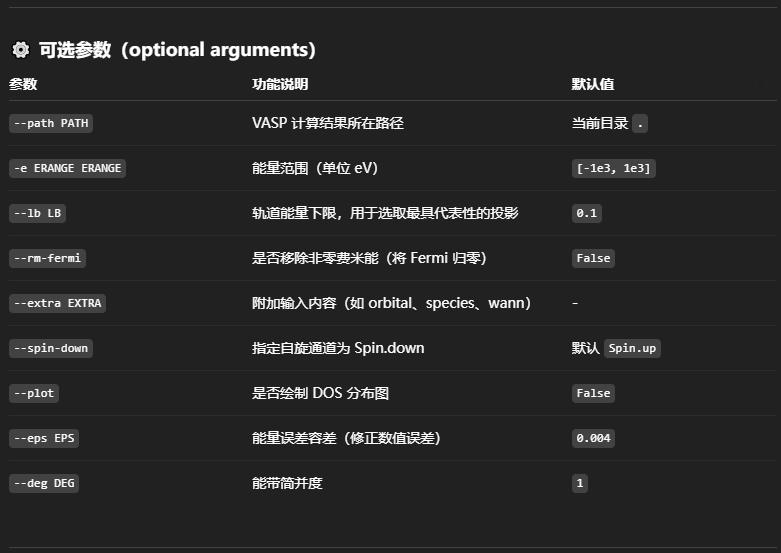
\includegraphics[max width=0.88\linewidth,max height=0.62\textheight,keepaspectratio]{assets/figure-9b5d250a7acc.png}
\end{figure}\par\par


\par\begin{figure}[H]\centering
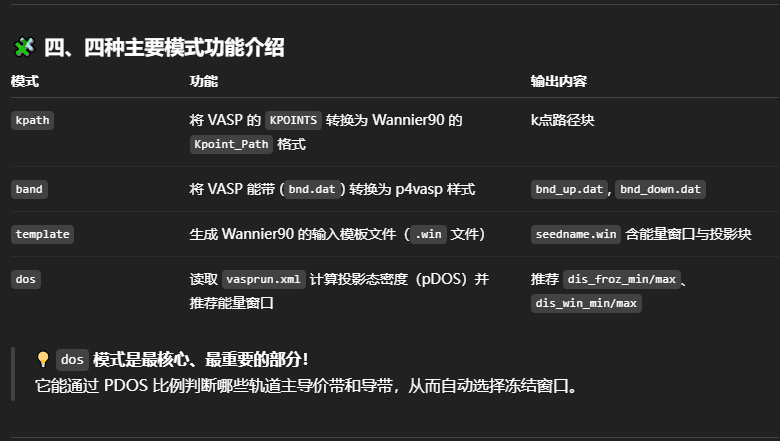
\includegraphics[max width=0.88\linewidth,max height=0.62\textheight,keepaspectratio]{assets/figure-2efdb1628035.png}
\end{figure}\par\par


\par\begin{figure}[H]\centering
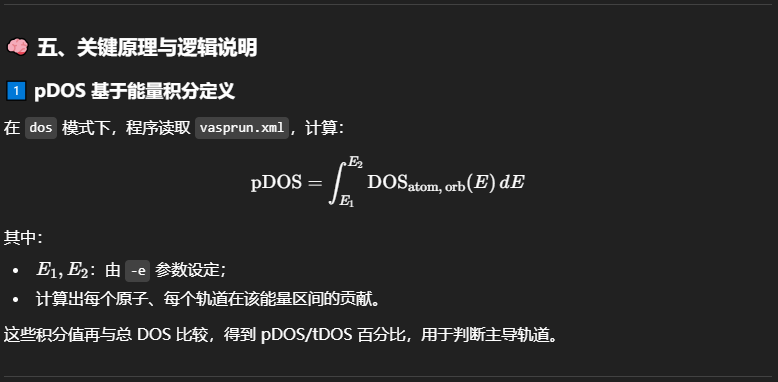
\includegraphics[max width=0.88\linewidth,max height=0.62\textheight,keepaspectratio]{assets/figure-545edba9c9dc.png}
\end{figure}\par\par


\par\begin{figure}[H]\centering
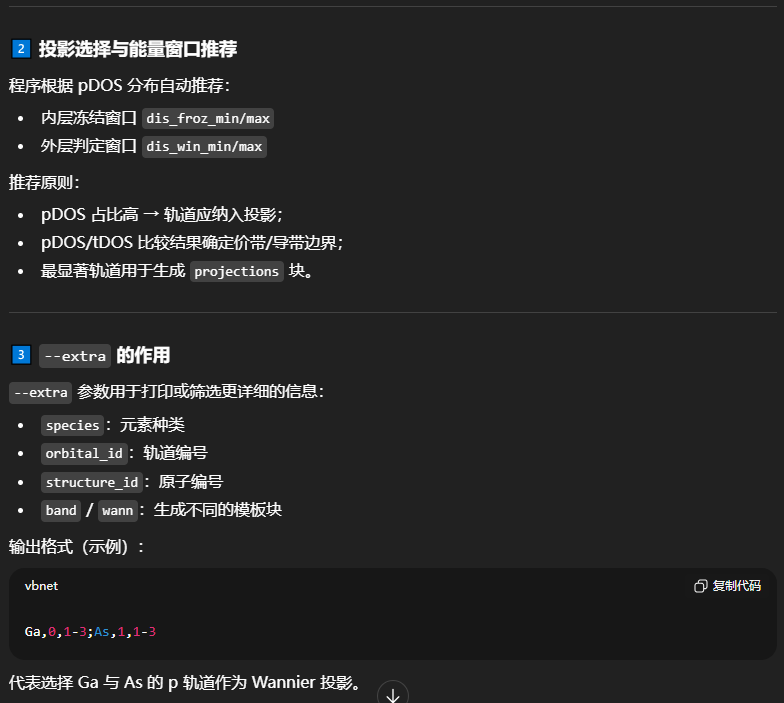
\includegraphics[max width=0.88\linewidth,max height=0.62\textheight,keepaspectratio]{assets/figure-10a6892da9c9.png}
\end{figure}\par\par


\par\begin{figure}[H]\centering

\includegraphics[max width=0.88\linewidth,max height=0.62\textheight,keepaspectratio]{assets/figure-9dbe5bc34d30.png}
\end{figure}\par\par


\par\begin{figure}[H]\centering
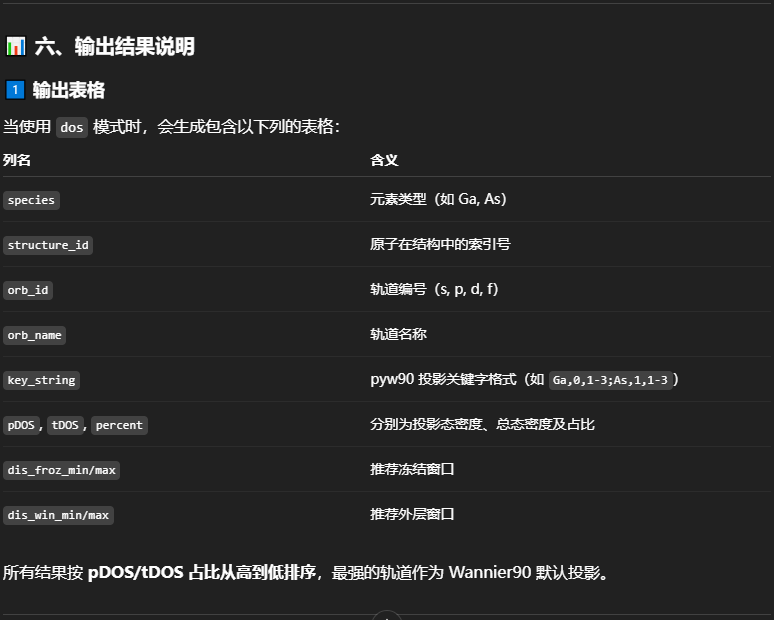
\includegraphics[max width=0.88\linewidth,max height=0.62\textheight,keepaspectratio]{assets/figure-965f8aa57509.png}
\end{figure}\par\par


\par\begin{figure}[H]\centering
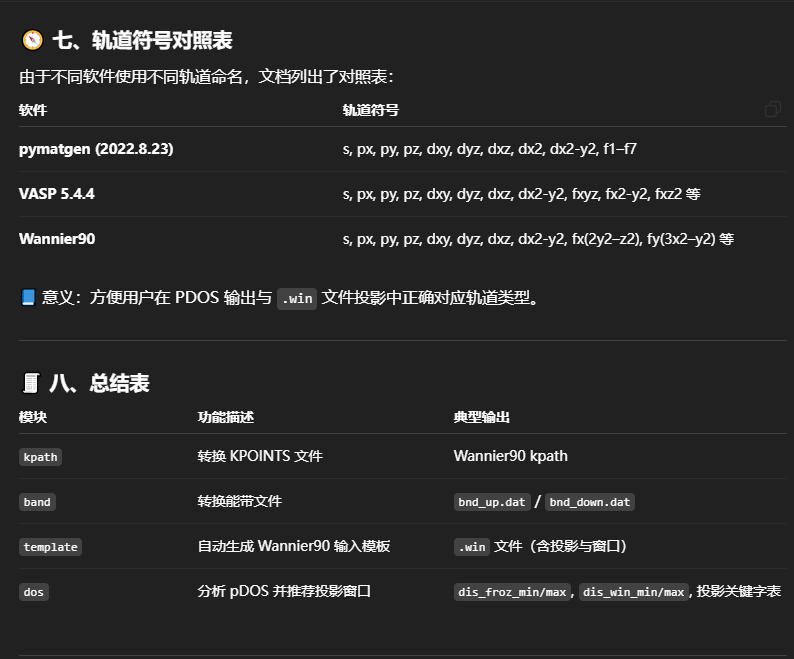
\includegraphics[max width=0.88\linewidth,max height=0.62\textheight,keepaspectratio]{assets/figure-64c4e6cbd068.png}
\end{figure}\par\par


\par\begin{figure}[H]\centering
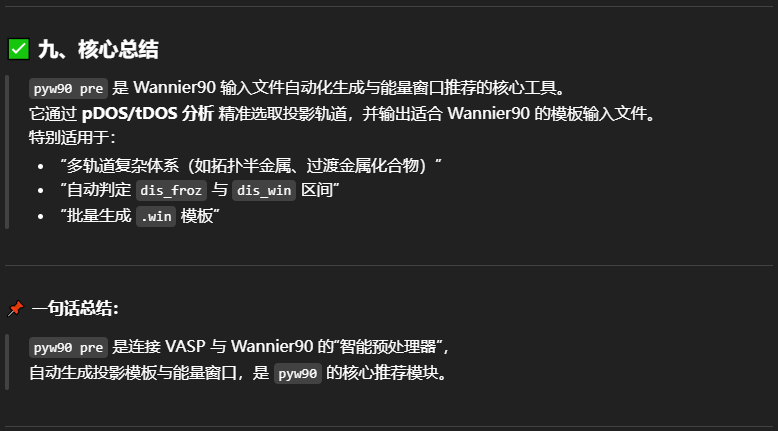
\includegraphics[max width=0.88\linewidth,max height=0.62\textheight,keepaspectratio]{assets/figure-689b0719d8d6.png}
\end{figure}\par\par



\section{pyw90的简介}
\begin{articlemeta}
\textbf{日期：}2025-11-27\hfill\textbf{在线原文：}\href{https://marx2001.github.io/sci-note\_posts/20251127-pyw2}{marx2001.github.io}
\end{articlemeta}

https:/\allowbreak{}/\allowbreak{}github.com/\allowbreak{}Cloudiiink/\allowbreak{}pyw90/\allowbreak{}blob/\allowbreak{}master/\allowbreak{}README.md\par


\subsubsection{简介}


\par\begin{figure}[H]\centering
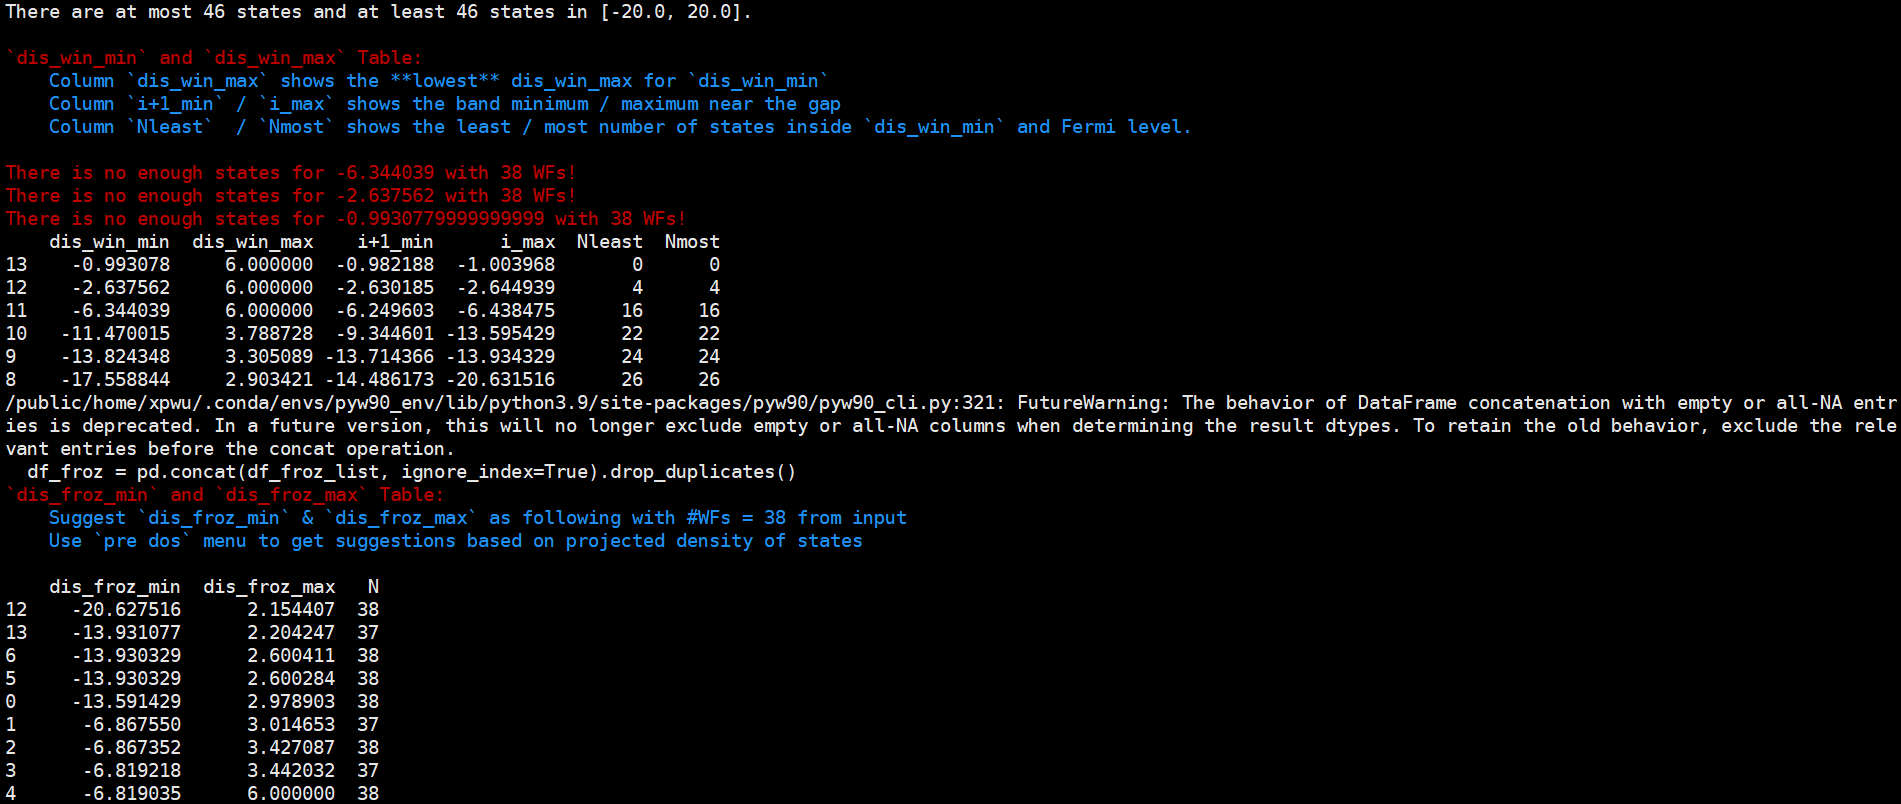
\includegraphics[max width=0.88\linewidth,max height=0.62\textheight,keepaspectratio]{assets/figure-8a1413195a63.png}
\end{figure}\par\par


\par\begin{figure}[H]\centering
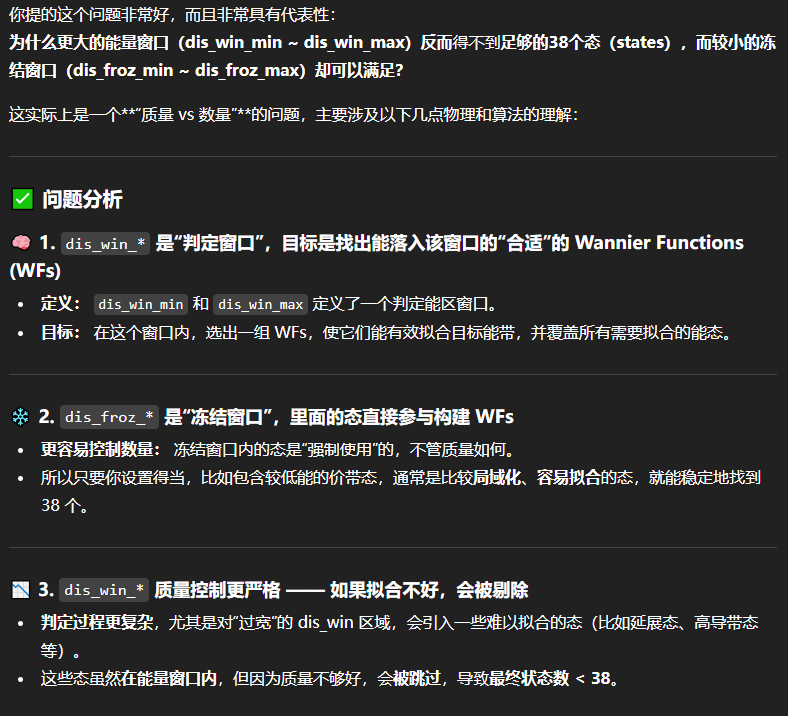
\includegraphics[max width=0.88\linewidth,max height=0.62\textheight,keepaspectratio]{assets/figure-833b6b235e2c.png}
\end{figure}\par\par


\par\begin{figure}[H]\centering
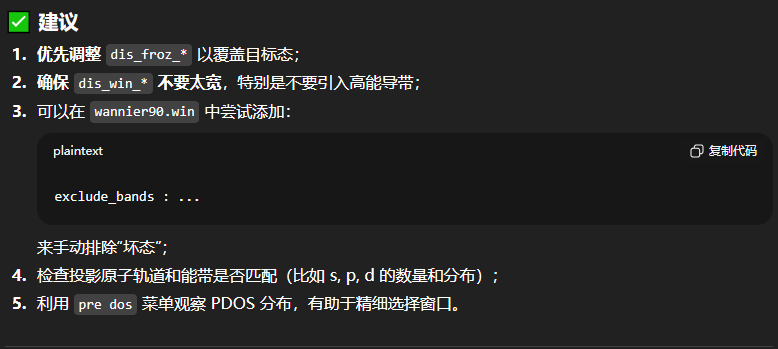
\includegraphics[max width=0.88\linewidth,max height=0.62\textheight,keepaspectratio]{assets/figure-b3072ee3b8e6.png}
\end{figure}\par\par


\par\begin{figure}[H]\centering
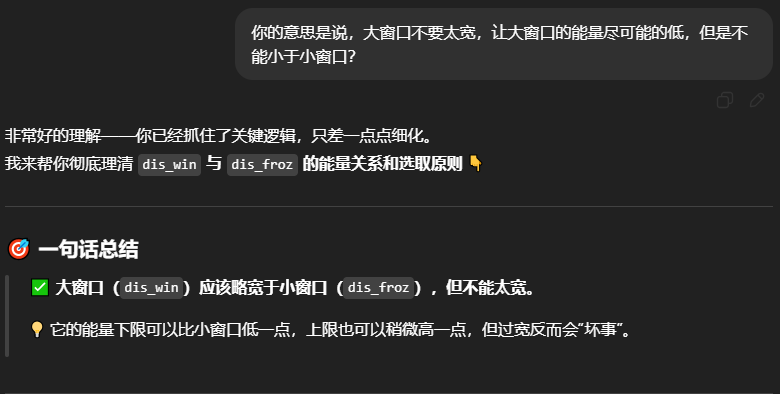
\includegraphics[max width=0.88\linewidth,max height=0.62\textheight,keepaspectratio]{assets/figure-6d31ad2d130f.png}
\end{figure}\par\par


\par\begin{figure}[H]\centering
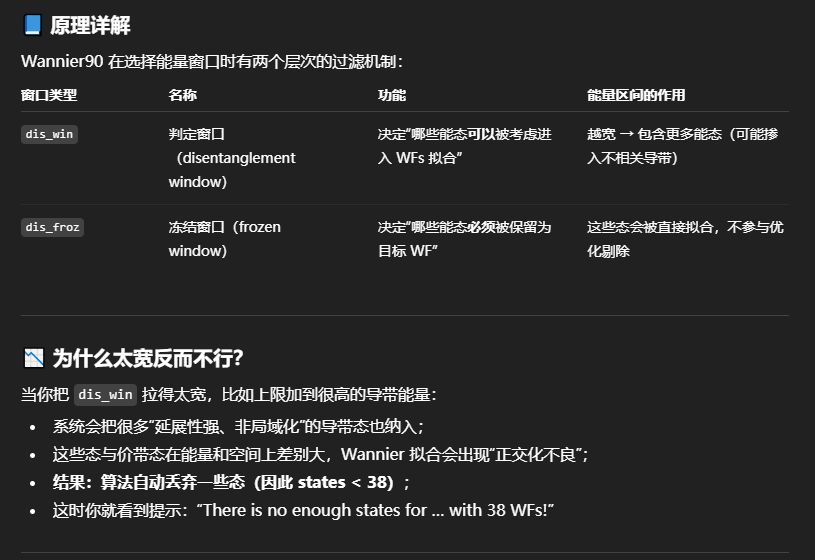
\includegraphics[max width=0.88\linewidth,max height=0.62\textheight,keepaspectratio]{assets/figure-197666d327dd.png}
\end{figure}\par\par


\par\begin{figure}[H]\centering
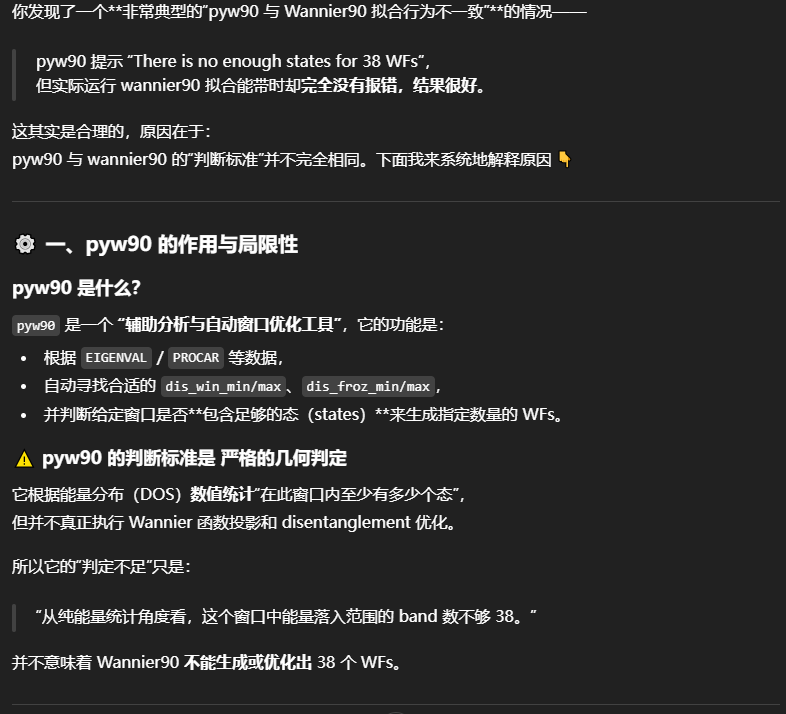
\includegraphics[max width=0.88\linewidth,max height=0.62\textheight,keepaspectratio]{assets/figure-4af6315b4fea.png}
\end{figure}\par\par



\section{wannier90的能带拟合步骤}
\begin{articlemeta}
\textbf{日期：}2025-11-27\hfill\textbf{在线原文：}\href{https://marx2001.github.io/sci-note\_posts/20251127-band}{marx2001.github.io}
\end{articlemeta}

\subsection{流程与步骤日志}


\subsubsection{1. static计算}


不开启ncl\par


k点取11,如下\par


\begin{codeindexbox}{代码清单 A.20.1}
语言：shell；完整代码见附录第 \pageref{code:20:1} 页，共 5 行。
\end{codeindexbox}


INCAR如下\par


\begin{codeindexbox}{代码清单 A.20.2}
语言：shell；完整代码见附录第 \pageref{code:20:2} 页，共 43 行。
\end{codeindexbox}


运行计算\par


获得结果并查看磁矩\par


\begin{codeindexbox}{代码清单 A.20.3}
语言：shell；完整代码见附录第 \pageref{code:20:3} 页，共 11 行。
\end{codeindexbox}


\subsubsection{2. bandsoc计算}


INCAR如下\par


\begin{codeindexbox}{代码清单 A.20.4}
语言：shell；完整代码见附录第 \pageref{code:20:4} 页，共 42 行。
\end{codeindexbox}


kpoints如下\par


\begin{codeindexbox}{代码清单 A.20.5}
语言：shell；完整代码见附录第 \pageref{code:20:5} 页，共 15 行。
\end{codeindexbox}


绘制投影能带(略)\par


\subsubsection{3. ncl\_\allowbreak{}Wannier90计算}


添加LWANNIER90=.T\par


以及WANNIER\_\allowbreak{}WIN和NBANDS=64以及NUM\_\allowbreak{}WANN=38的tag,其它的参数参考ncl的设置方式进行修改\par


NCORE=4注释掉\par


\begin{codeindexbox}{代码清单 A.20.6}
语言：shell；完整代码见附录第 \pageref{code:20:6} 页，共 54 行。
\end{codeindexbox}


体系不易收敛,可以尝试开启输出波函数和电荷密度方便续算.\par


\subsubsection{4. 能带拟合}


后续过程见之前的Bi烯教程中的相应部分的内容\par


\subsection{Results}


\begin{codeindexbox}{代码清单 A.20.7}
语言：shell；完整代码见附录第 \pageref{code:20:7} 页，共 10 行。
\end{codeindexbox}


结果不太对,判断为构建紧束缚模型的时候可能考虑了多余的轨道,导致既有陈数又有Z2.\par


如果static是线性计算的,看看是否会有影响。(因为之前用的线性计算的static的chgcar,并未出现陈数和z2数同时出现的情况)\par


问题同样出现,应该是拟合轨道数目的问题,新版本wannier可能对轨道的严格性做了提升,1.2的版本可以正常计算出Z2拓扑不变量。\par


\subsection{选择合适的轨道的结果}


遇到一个情况,启动第三步,静态ncl+LWANNIER90=.T的时候,一定要先清理上次计算剩下的输出文件mmn等,并删掉win文件中上次计算vasp生成的部分,然后重新启动计算,这样能保证输出正 确,减少遇到非主流报错的可能性。\par



\section{pyw90的测试用例}
\begin{articlemeta}
\textbf{日期：}2025-11-28\hfill\textbf{在线原文：}\href{https://marx2001.github.io/sci-note\_posts/20251128-pyw-test}{marx2001.github.io}
\end{articlemeta}

https:/\allowbreak{}/\allowbreak{}github.com/\allowbreak{}Cloudiiink/\allowbreak{}pyw90/\allowbreak{}blob/\allowbreak{}master/\allowbreak{}README.md\par


创建虚拟环境\par


\begin{inlinecodebox}{命令示例 · shell}
\VerbatimInput[fontsize=\small,breaklines=true,breakanywhere=true,tabsize=2,listparameters={\setlength{\topsep}{0pt}\setlength{\partopsep}{0pt}\setlength{\parsep}{0pt}}]{code/021-001.sh}
\end{inlinecodebox}


激活环境 并安装\par


\begin{codeindexbox}{代码清单 A.21.2}
语言：shell；完整代码见附录第 \pageref{code:21:2} 页，共 8 行。
\end{codeindexbox}


\subsubsection{流程与步骤}


例子选取于上方网址,作为学习交流使用,切勿用作他途。\par


以下假设已熟悉 Wannier90,并已按下方示例准备文件夹。该结构仅作示例;实际操作时,命令在能带计算文件夹中运行。\par


\begin{codeindexbox}{代码清单 A.21.3}
语言：shell；完整代码见附录第 \pageref{code:21:3} 页，共 15 行。
\end{codeindexbox}


通过eig菜单显示特征值分布:\par


\begin{codeindexbox}{代码清单 A.21.4}
语言：shell；完整代码见附录第 \pageref{code:21:4} 页，共 1 行。
\end{codeindexbox}


结果为:\par


\begin{codeindexbox}{代码清单 A.21.5}
语言：shell；完整代码见附录第 \pageref{code:21:5} 页，共 23 行。
\end{codeindexbox}


也可以将结果输出为pdf格式,且是某个波段的能量分布到文件夹中。\par


运行下方指令得到一些关于能量窗口的建议:\par


\begin{codeindexbox}{代码清单 A.21.6}
语言：shell；完整代码见附录第 \pageref{code:21:6} 页，共 1 行。
\end{codeindexbox}


结果:\par


\begin{codeindexbox}{代码清单 A.21.7}
语言：shell；完整代码见附录第 \pageref{code:21:7} 页，共 24 行。
\end{codeindexbox}


运行指令得到建议投影的轨道并产生wannier90.in。\par


此处,我们选择费米能级附近 [-1, 1] eV 的能量区间进行评估,以得出最具代表性的投影权重建议\par


也可以通过调整相应参数来修改能量区间的选择下限,以观察输出结果的变化。\par


\begin{codeindexbox}{代码清单 A.21.8}
语言：shell；完整代码见附录第 \pageref{code:21:8} 页，共 2 行。
\end{codeindexbox}


结果:\par


\begin{codeindexbox}{代码清单 A.21.9}
语言：shell；完整代码见附录第 \pageref{code:21:9} 页，共 78 行。
\end{codeindexbox}


尝试修改上下限:\par


\begin{codeindexbox}{代码清单 A.21.10}
语言：shell；完整代码见附录第 \pageref{code:21:10} 页，共 1 行。
\end{codeindexbox}


\begin{codeindexbox}{代码清单 A.21.11}
语言：shell；完整代码见附录第 \pageref{code:21:11} 页，共 76 行。
\end{codeindexbox}


可以看出拟合能带的能量范围不同,投影轨道的数目也不同。\par


随后,我们可以将能量范围调整至一个非常大的区间:\par


\begin{codeindexbox}{代码清单 A.21.12}
语言：shell；完整代码见附录第 \pageref{code:21:12} 页，共 1 行。
\end{codeindexbox}


其中,第一个“1-2”是Nb的原子编号,“4-8”为轨道编号,其余元素的格式同理。上一步中的靠后部分有这些编号的output\par


结果为:\par


\begin{codeindexbox}{代码清单 A.21.13}
语言：shell；完整代码见附录第 \pageref{code:21:13} 页，共 35 行。
\end{codeindexbox}


轨道编号参考(vasp5.4.4与vasp6.4.3应当相同)\par


\begin{codeindexbox}{代码清单 A.21.14}
语言：shell；完整代码见附录第 \pageref{code:21:14} 页，共 12 行。
\end{codeindexbox}


由此,我们获得了Wannier函数的初始猜测。随后,我们可以使用命令 pyw90 pre template –extra basic来为 Wannier90 与 VASP 的接口生成 .wannier90.win模板文件。\par


由于(VASP版本 <6.0)仅支持 Wannier90 1.2 版本的接口。可能需要修改并重新编译接口代码,使其能够计算非共线Wannier函数并支持旋量投影方法。更多详细信息,请参考项目: Chengcheng-Xiao/\allowbreak{}VASP2WAN90\_\allowbreak{}v2\_\allowbreak{}fix(一个更新版的VASP2WANNIER90v2接口)。\par


\begin{center}\small
\begin{longtable}{@{}p{0.400\textwidth} p{0.400\textwidth}@{}}
\toprule
此处由于不识别“ & ”符号,所以可以手写win文件: \\
\midrule
\bottomrule
\end{longtable}
\end{center}


\begin{codeindexbox}{代码清单 A.21.15}
语言：shell；完整代码见附录第 \pageref{code:21:15} 页，共 12 行。
\end{codeindexbox}


此文件 (wannier90.win) 需在 wannier文件夹内创建。同时,必须在 INCAR文件中设置 LWANNIER90 = .TRUE.以启用 VASP与 Wannier90之间的接口。\par


此功能(VASP-Wannier90接口)仅在 VASP 编译时启用了 -DVASP2WANNIER90或 -DVASP2WANNIER90v2选项才可用。\par


其他输入参数(如 kpoints- k点列表,atoms- 原子位置,unit\_\allowbreak{}cell- 晶胞矢量,mp\_\allowbreak{}grid- Monkhorst-Pack网格尺寸等)将基于 VASP计算的信息自动设置。\par


对于 VASP (>= 6.2.0) 版本,它将支持 Wannier90>=3.0。并且,wannier90.win输入文件的内容可以直接通过 INCAR文件中的 WANNIER90\_\allowbreak{}WIN参数输入(参见 Vaspwiki 上的 WANNIER90\_\allowbreak{}WIN 条目),不再需要单独的初始 wannier90.win文件。\par


执行计算任务后,VASP会为后续的 WANNIER90运行写入所需的输入文件:wannier90.win, wannier90.mmn, wannier90.eig以及 wannier90.amn。\par


这里我们将 disentanglement (dis) 能量窗口的初始猜测和能带结构计算的路径卡片写入 wannier90.win文件。其中 Kpoint\_\allowbreak{}Path模块可以通过命令 pyw90 pre kpath –path ../\allowbreak{}bnd生成(此命令可能利用之前能带计算 ../\allowbreak{}bnd的路径信息)。\par


开始第一次wannier90能带拟合,具体过程参考之前的教程\par


\begin{codeindexbox}{代码清单 A.21.16}
语言：shell；完整代码见附录第 \pageref{code:21:16} 页，共 12 行。
\end{codeindexbox}


我使用的是vasp6.4.3的版本,写在INCAR内即可,不需要单独的win文件。\par


随后,我们可以使用 pyw90 auto菜单来自动优化 disentanglement 能量窗口。配置文件应使用 pyw90 auto input命令生成。在运行计算之前,请自定义该配置文件(有关每个参数键的含义, 请参阅该菜单的文档)。\par


先进行wannier90的能带拟合,得到wannier90\_\allowbreak{}band.dat等等文件。\par


准备好所有输入文件后,键入 pyw90 auto run来执行该流程。会产生两个输出文件。\par


我们一步一步进行。\par


先运行脚本\par


\begin{codeindexbox}{代码清单 A.21.17}
语言：shell；完整代码见附录第 \pageref{code:21:17} 页，共 1 行。
\end{codeindexbox}


产生auto\_\allowbreak{}w90\_\allowbreak{}input.yaml文件,修改其中的内容与slurm系统的匹配\par


再修改yml文件中的参数\par


\begin{codeindexbox}{代码清单 A.21.18}
语言：shell；完整代码见附录第 \pageref{code:21:18} 页，共 2 行。
\end{codeindexbox}


或\par


\begin{codeindexbox}{代码清单 A.21.19}
语言：shell；完整代码见附录第 \pageref{code:21:19} 页，共 2 行。
\end{codeindexbox}


编辑提交任务脚本w90.script\par


\begin{codeindexbox}{代码清单 A.21.20}
语言：shell；完整代码见附录第 \pageref{code:21:20} 页，共 42 行。
\end{codeindexbox}


然后运行自动分析程序\par


\begin{codeindexbox}{代码清单 A.21.21}
语言：shell；完整代码见附录第 \pageref{code:21:21} 页，共 1 行。
\end{codeindexbox}


等待即可。\par


此刻凌晨3:20了,稍后睡醒再写一篇如何修改正确参数来进行能量窗口计算的文章。\par


补充,最后一步,利用命令生成可视化的DFT计算能带与pyw90结果的对比\par


\begin{codeindexbox}{代码清单 A.21.22}
语言：shell；完整代码见附录第 \pageref{code:21:22} 页，共 1 行。
\end{codeindexbox}


yaml文件中有kernel的设置,efermi可以自己寻找\par


备注:如果没有bnd.dat文件,运行指令产生\par


\begin{codeindexbox}{代码清单 A.21.23}
语言：shell；完整代码见附录第 \pageref{code:21:23} 页，共 1 行。
\end{codeindexbox}



\section{pyw90的测试用例2\_\allowbreak{}本地运行}
\begin{articlemeta}
\textbf{日期：}2025-11-28\hfill\textbf{在线原文：}\href{https://marx2001.github.io/sci-note\_posts/20251128-pyw-auto}{marx2001.github.io}
\end{articlemeta}

https:/\allowbreak{}/\allowbreak{}github.com/\allowbreak{}Cloudiiink/\allowbreak{}pyw90/\allowbreak{}blob/\allowbreak{}master/\allowbreak{}README.md\par


首先以任意窗口成功地运行一次weannier90,得到wannier90\_\allowbreak{}band.dat文件。准备好auto\_\allowbreak{}w90\_\allowbreak{}input.yaml文件。\par


修改auto\_\allowbreak{}w90\_\allowbreak{}input.yaml文件中的代码为:\par


\begin{codeindexbox}{代码清单 A.22.1}
语言：shell；完整代码见附录第 \pageref{code:22:1} 页，共 20 行。
\end{codeindexbox}


然后运行,这个要在band计算的文件夹中运行才能得到正确的bnd.dat,大小应该和BAND.dat文件相差不大\par


\begin{codeindexbox}{代码清单 A.22.2}
语言：shell；完整代码见附录第 \pageref{code:22:2} 页，共 1 行。
\end{codeindexbox}


得到vasp计算的bnd.dat文件\par


再运行\par


\begin{codeindexbox}{代码清单 A.22.3}
语言：shell；完整代码见附录第 \pageref{code:22:3} 页，共 1 行。
\end{codeindexbox}


设置窗口的技巧,能量上下限减去费米能级,即为origin作图的能带图的能量范围,可以根据dft计算的能量范围设计每一次迭代的能量上下限。\par


得到结果后,修改yml文件中的窗口范围,然后改变固定窗口,比如原来固定小窗口,优化大窗口,同时也要修改窗口变化的范围,大概看一眼能带,选择合适的区间\par


经过一些测试,我发现固定两个窗口的min,优化max窗口的位置似乎是一个不错的开始,因为我们可以在gap处设置好min,可以保证这个min的数值没有问题,然后比较难搞的上窗口通过迭代方式 优化得到。\par


以上为暂时的最终的程序使用方法和心得体会。\par


流程梳理:\par


\begin{enumerate}
\item static计算得到CHGCAR\par
\item bandsoc计算得到bnd.dat\par
\item wannier90的能带拟合,一定要确定好min窗口所在的能量,记得减去费米能级对照origin画的能带图确定min窗口所在的能量值\par
\item 运行pyw90进行上窗口能量优化,如果中途计算因为包含的state不足而停掉,那么需要重新修改yaml的窗口和win文件的窗口匹配,检查好yaml内能量窗口的变化的范围。\par
\item 重复上述步骤3、4,直到能带完全对应。\par
\end{enumerate}


\begin{codeindexbox}{代码清单 A.22.4}
语言：shell；完整代码见附录第 \pageref{code:22:4} 页，共 1 行。
\end{codeindexbox}


yaml文件中有kernel的设置,efermi可以自己寻找\par


备注:如果没有bnd.dat文件,运行指令产生\par


\begin{codeindexbox}{代码清单 A.22.5}
语言：shell；完整代码见附录第 \pageref{code:22:5} 页，共 1 行。
\end{codeindexbox}


终止任务\par


\begin{codeindexbox}{代码清单 A.22.6}
语言：shell；完整代码见附录第 \pageref{code:22:6} 页，共 1 行。
\end{codeindexbox}


或者\par


\begin{codeindexbox}{代码清单 A.22.7}
语言：shell；完整代码见附录第 \pageref{code:22:7} 页，共 1 行。
\end{codeindexbox}



\section{Wannier Tools的代码解释}
\begin{articlemeta}
\textbf{日期：}2025-12-02\hfill\textbf{在线原文：}\href{https://marx2001.github.io/sci-note\_posts/20251202-code}{marx2001.github.io}
\end{articlemeta}

创建虚拟环境\par


\begin{codeindexbox}{代码清单 A.23.1}
语言：fortran；完整代码见附录第 \pageref{code:23:1} 页，共 2051 行。
\end{codeindexbox}


\begin{codeindexbox}{代码清单 A.23.2}
语言：fortran；完整代码见附录第 \pageref{code:23:2} 页，共 290 行。
\end{codeindexbox}



\section{wannierberrier的安装}
\begin{articlemeta}
\textbf{日期：}2025-12-03\hfill\textbf{在线原文：}\href{https://marx2001.github.io/sci-note\_posts/20251203-wann}{marx2001.github.io}
\end{articlemeta}

\subsection{Recording}


\subsubsection{1. 步骤}


创建虚拟环境\par


\begin{inlinecodebox}{命令示例 · shell}
\VerbatimInput[fontsize=\small,breaklines=true,breakanywhere=true,tabsize=2,listparameters={\setlength{\topsep}{0pt}\setlength{\partopsep}{0pt}\setlength{\parsep}{0pt}}]{code/024-001.sh}
\end{inlinecodebox}


使用清华源安装\par


\begin{codeindexbox}{代码清单 A.24.2}
语言：shell；完整代码见附录第 \pageref{code:24:2} 页，共 9 行。
\end{codeindexbox}


查看所需依赖的版本:\par


\begin{inlinecodebox}{命令示例 · shell}
\VerbatimInput[fontsize=\small,breaklines=true,breakanywhere=true,tabsize=2,listparameters={\setlength{\topsep}{0pt}\setlength{\partopsep}{0pt}\setlength{\parsep}{0pt}}]{code/024-003.sh}
\end{inlinecodebox}


装完环境重启一下shell面板,会更新python的版本显示。\par


修改并更新知乎中的代码,还需要安装FFT等库,安装很简单,就不在此一一列出了。\par


目前的代码是大概正确的,报错是因为晶格常数不完全对称,但是没有找到代码中调整tolerance的api,所以我用高对称性结构重新加入wannier接口拟合一遍。 第一版代码,存在报错,这是为了记录,可以及时进行版本回退\par


\begin{codeindexbox}{代码清单 A.24.4}
语言：shell；完整代码见附录第 \pageref{code:24:4} 页，共 93 行。
\end{codeindexbox}



\section{wansymm的对称化功能}
\begin{articlemeta}
\textbf{日期：}2025-12-03\hfill\textbf{在线原文：}\href{https://marx2001.github.io/sci-note\_posts/20251203-wannberrier}{marx2001.github.io}
\end{articlemeta}

\subsection{Recording}


\subsubsection{1. 步骤}


其余步骤同知乎上文章https:/\allowbreak{}/\allowbreak{}zhuanlan.zhihu.com/\allowbreak{}p/\allowbreak{}675502389和https:/\allowbreak{}/\allowbreak{}zhuanlan.zhihu.com/\allowbreak{}p/\allowbreak{}675502472,但是build文件夹内并没有出现lib,所以我把路径放到lib64文件夹中,即在配置变量这个步骤 中,把路径指定到lib64文件夹,而不是知乎上写的build/\allowbreak{}lib。\par


给命令授权:wannsymm.x ,在cssong目录中的bashrc内添加环境变量的路径即可。\par


\begin{inlinecodebox}{命令示例 · shell}
\VerbatimInput[fontsize=\small,breaklines=true,breakanywhere=true,tabsize=2,listparameters={\setlength{\topsep}{0pt}\setlength{\partopsep}{0pt}\setlength{\parsep}{0pt}}]{code/025-001.sh}
\end{inlinecodebox}


\begin{inlinecodebox}{命令示例 · shell}
\VerbatimInput[fontsize=\small,breaklines=true,breakanywhere=true,tabsize=2,listparameters={\setlength{\topsep}{0pt}\setlength{\partopsep}{0pt}\setlength{\parsep}{0pt}}]{code/025-002.sh}
\end{inlinecodebox}


没节点了,直接管理节点上用1核跑\par


\begin{inlinecodebox}{命令示例 · shell}
\VerbatimInput[fontsize=\small,breaklines=true,breakanywhere=true,tabsize=2,listparameters={\setlength{\topsep}{0pt}\setlength{\partopsep}{0pt}\setlength{\parsep}{0pt}}]{code/025-003.sh}
\end{inlinecodebox}


绘图脚本记录:\par


\begin{inlinecodebox}{命令示例 · shell}
\VerbatimInput[fontsize=\small,breaklines=true,breakanywhere=true,tabsize=2,listparameters={\setlength{\topsep}{0pt}\setlength{\partopsep}{0pt}\setlength{\parsep}{0pt}}]{code/025-004.sh}
\end{inlinecodebox}


正式开始计算:\par


\begin{enumerate}
\item 采用模板,ws.in,进行第一步计算:
\end{enumerate}


\begin{codeindexbox}{代码清单 A.25.5}
语言：python；完整代码见附录第 \pageref{code:25:5} 页，共 19 行。
\end{codeindexbox}


\begin{enumerate}
\item 第二步加入高对称点路径
\end{enumerate}


加入restart = T 绘制对称化后的能带\par


\begin{codeindexbox}{代码清单 A.25.6}
语言：python；完整代码见附录第 \pageref{code:25:6} 页，共 9 行。
\end{codeindexbox}



\section{利用Wannier Tools的对称化hr.dat}
\begin{articlemeta}
\textbf{日期：}2025-12-14\hfill\textbf{在线原文：}\href{https://marx2001.github.io/sci-note\_posts/20251215-wt-sym}{marx2001.github.io}
\end{articlemeta}

\subsection{Tutorials-irvsp补充和指令}


\subsubsection{简介}


确保hr.dat仍保留DFT计算中的对称性,这样能保证wannier90的计算结果是正确的\par


\subsection{流程}


\begin{enumerate}
\item 准备POSCAR\par
\item 判断空间群:\par
\end{enumerate}


\begin{inlinecodebox}{命令示例 · shell}
\VerbatimInput[fontsize=\small,breaklines=true,breakanywhere=true,tabsize=2,listparameters={\setlength{\topsep}{0pt}\setlength{\partopsep}{0pt}\setlength{\parsep}{0pt}}]{code/026-001.sh}
\end{inlinecodebox}


然后\par


\begin{inlinecodebox}{命令示例 · shell}
\VerbatimInput[fontsize=\small,breaklines=true,breakanywhere=true,tabsize=2,listparameters={\setlength{\topsep}{0pt}\setlength{\partopsep}{0pt}\setlength{\parsep}{0pt}}]{code/026-002.sh}
\end{inlinecodebox}


判断空间群\par


\begin{enumerate}
\item 复制新POSCAR,再做计算静态自洽、能带计算
\end{enumerate}


\subsection{Wannier Tools对称化}


\begin{enumerate}
\item 准备输入文件locaxis.in
\end{enumerate}


\begin{codeindexbox}{代码清单 A.26.3}
语言：python；完整代码见附录第 \pageref{code:26:3} 页，共 24 行。
\end{codeindexbox}


采用晶格对称性,设置line 20为0,即不读取原子坐标系。\par


准备poscar.in,内容:\par


\begin{codeindexbox}{代码清单 A.26.4}
语言：python；完整代码见附录第 \pageref{code:26:4} 页，共 13 行。
\end{codeindexbox}


复制poscar进去。\par


对应的轨道,准备文件wann.in\par


\begin{codeindexbox}{代码清单 A.26.5}
语言：python；完整代码见附录第 \pageref{code:26:5} 页，共 30 行。
\end{codeindexbox}


准备wannier90.in文件,内容:\par


\begin{codeindexbox}{代码清单 A.26.6}
语言：python；完整代码见附录第 \pageref{code:26:6} 页，共 70 行。
\end{codeindexbox}


准备hr.dat文件,未对称化的。\par


\begin{enumerate}
\item 激活环境,运行程序
\end{enumerate}


\begin{inlinecodebox}{命令示例 · shell}
\VerbatimInput[fontsize=\small,breaklines=true,breakanywhere=true,tabsize=2,listparameters={\setlength{\topsep}{0pt}\setlength{\partopsep}{0pt}\setlength{\parsep}{0pt}}]{code/026-007.sh}
\end{inlinecodebox}


运行程序\par


\begin{inlinecodebox}{命令示例 · shell}
\VerbatimInput[fontsize=\small,breaklines=true,breakanywhere=true,tabsize=2,listparameters={\setlength{\topsep}{0pt}\setlength{\partopsep}{0pt}\setlength{\parsep}{0pt}}]{code/026-008.sh}
\end{inlinecodebox}


记得把python库和上面的symmhr\_\allowbreak{}addrptblock.py放到一个文件夹内,要不然运行不了\par


看日志,没有报错的话,就得到了最终的hr.dat\par


要用wannier1.2版本。\par


\chapter{紧束缚、拓扑与磁性软件}
\begin{partbox}本专题收录 13 篇文章。\end{partbox}

\section{tb2j计算磁参数的DMI计算}
\begin{articlemeta}
\textbf{日期：}2025-11-26\hfill\textbf{在线原文：}\href{https://marx2001.github.io/sci-note\_posts/20251126-DMI-tb2j}{marx2001.github.io}
\end{articlemeta}

\subsection{Recording}


对于tb2j的0.7版本,DMI体现在原子对内,并无如同四态法一样的计算形式,所以需要手动推导每一个原子对的DMI大小。\par


\begin{enumerate}
\item 首先找到两个原子的相对位置,对应的原子对,做中垂线\par
\item 找到两个原子间的DMI坐标形式的强度分布,对这个中垂线做投影,相加即为D/\allowbreak{}/\allowbreak{}的大小\par
\item Dz就是绝对值大小,因为在二维投影上是一个点\par
\end{enumerate}



\section{TB2J新版测试}
\begin{articlemeta}
\textbf{日期：}2025-11-27\hfill\textbf{在线原文：}\href{https://marx2001.github.io/sci-note\_posts/20251127-tb2j-1}{marx2001.github.io}
\end{articlemeta}

TB2J0.9.0+Wannier3.1.0+vasp6.4.3\par


\subsection{Recording}


\subsubsection{1. 查看tb2j版本}


\begin{inlinecodebox}{命令示例 · shell}
\VerbatimInput[fontsize=\small,breaklines=true,breakanywhere=true,tabsize=2,listparameters={\setlength{\topsep}{0pt}\setlength{\partopsep}{0pt}\setlength{\parsep}{0pt}}]{code/028-001.sh}
\end{inlinecodebox}


新0.7.2.1版本的tb2j安装:\par


创建环境\par


\begin{inlinecodebox}{命令示例 · shell}
\VerbatimInput[fontsize=\small,breaklines=true,breakanywhere=true,tabsize=2,listparameters={\setlength{\topsep}{0pt}\setlength{\partopsep}{0pt}\setlength{\parsep}{0pt}}]{code/028-002.sh}
\end{inlinecodebox}


进入环境:\par


\begin{inlinecodebox}{命令示例 · shell}
\VerbatimInput[fontsize=\small,breaklines=true,breakanywhere=true,tabsize=2,listparameters={\setlength{\topsep}{0pt}\setlength{\partopsep}{0pt}\setlength{\parsep}{0pt}}]{code/028-003.sh}
\end{inlinecodebox}


现升级为tb2j0.9.0版本。\par


\begin{inlinecodebox}{命令示例 · shell}
\VerbatimInput[fontsize=\small,breaklines=true,breakanywhere=true,tabsize=2,listparameters={\setlength{\topsep}{0pt}\setlength{\partopsep}{0pt}\setlength{\parsep}{0pt}}]{code/028-004.sh}
\end{inlinecodebox}


0.7.1.1版本的环境进入方法:\par


\begin{inlinecodebox}{命令示例 · shell}
\VerbatimInput[fontsize=\small,breaklines=true,breakanywhere=true,tabsize=2,listparameters={\setlength{\topsep}{0pt}\setlength{\partopsep}{0pt}\setlength{\parsep}{0pt}}]{code/028-005.sh}
\end{inlinecodebox}


\subsubsection{2. 运行}


\begin{inlinecodebox}{命令示例 · shell}
\VerbatimInput[fontsize=\small,breaklines=true,breakanywhere=true,tabsize=2,listparameters={\setlength{\topsep}{0pt}\setlength{\partopsep}{0pt}\setlength{\parsep}{0pt}}]{code/028-006.sh}
\end{inlinecodebox}


自行修改合适的区间\par


\subsubsection{3. 如果配体的自旋磁动量不可忽略,需要downfolding海森堡哈密顿量}


先:\par


\begin{inlinecodebox}{命令示例 · shell}
\VerbatimInput[fontsize=\small,breaklines=true,breakanywhere=true,tabsize=2,listparameters={\setlength{\topsep}{0pt}\setlength{\partopsep}{0pt}\setlength{\parsep}{0pt}}]{code/028-007.sh}
\end{inlinecodebox}


结果保存到TB2J\_\allowbreak{}results目录后,运行downfolding功能,得到仅有Cr有效交换参数:\par


\begin{inlinecodebox}{命令示例 · shell}
\VerbatimInput[fontsize=\small,breaklines=true,breakanywhere=true,tabsize=2,listparameters={\setlength{\topsep}{0pt}\setlength{\partopsep}{0pt}\setlength{\parsep}{0pt}}]{code/028-008.sh}
\end{inlinecodebox}


文件夹中的文件要有POSCAR、POTCAR、xyz、hr.dat或tb.dat(某些版本的tb2j可以识别,见官方文档)、win文件等等,主要是dat文件,都放上也没坏处。\par


\subsection{Results}


上一模块是简要的过程记录,下面是结果比对,包括新老版本的\par


首先用0.7.1.1的版本进行测试:\par


进入环境:\par


\begin{inlinecodebox}{命令示例 · shell}
\VerbatimInput[fontsize=\small,breaklines=true,breakanywhere=true,tabsize=2,listparameters={\setlength{\topsep}{0pt}\setlength{\partopsep}{0pt}\setlength{\parsep}{0pt}}]{code/028-009.sh}
\end{inlinecodebox}


运行命令:\par


\begin{inlinecodebox}{命令示例 · shell}
\VerbatimInput[fontsize=\small,breaklines=true,breakanywhere=true,tabsize=2,listparameters={\setlength{\topsep}{0pt}\setlength{\partopsep}{0pt}\setlength{\parsep}{0pt}}]{code/028-010.sh}
\end{inlinecodebox}


得到结果\par


其它命令:\par


求平均值:\par


\begin{inlinecodebox}{命令示例 · shell}
\VerbatimInput[fontsize=\small,breaklines=true,breakanywhere=true,tabsize=2,listparameters={\setlength{\topsep}{0pt}\setlength{\partopsep}{0pt}\setlength{\parsep}{0pt}}]{code/028-011.sh}
\end{inlinecodebox}


求磁耦合参数:\par


\begin{inlinecodebox}{命令示例 · shell}
\VerbatimInput[fontsize=\small,breaklines=true,breakanywhere=true,tabsize=2,listparameters={\setlength{\topsep}{0pt}\setlength{\partopsep}{0pt}\setlength{\parsep}{0pt}}]{code/028-012.sh}
\end{inlinecodebox}


得到结果如下,体系为交错磁,而计算结果显示z方向磁矩为铁磁,我认为紧束缚模型可能有问题,需要重新拟合。升级了wannier90版本之后,也有许多新问题出现,比如一样的能量窗口,拟合 结果也对的上,但是k点由5\emph{5}1变为22\emph{22}11之后出现表面态等结果不对等问题,而且k点到超过13\emph{13}1之后,会出现开发者才能遇到的问题(报错中的信息是这么写的),报错内容是k点矢量方向变化,按照chatgpt5.1的建议修改为偶数个k点后,可以正常计算。\par


\par\begin{figure}[H]\centering
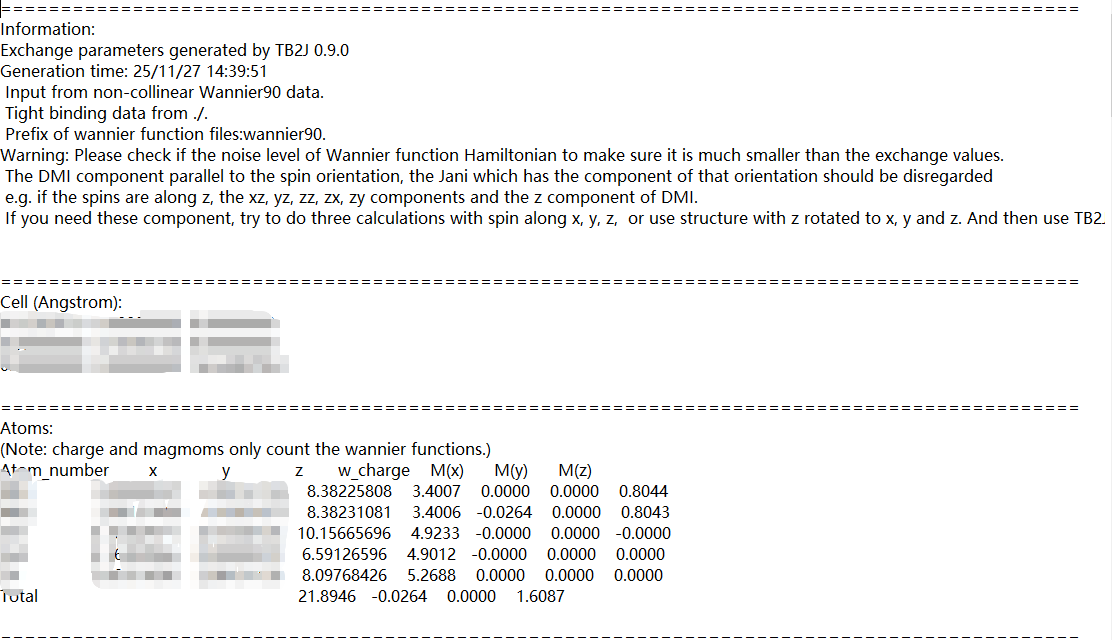
\includegraphics[max width=0.88\linewidth,max height=0.62\textheight,keepaspectratio]{assets/figure-4b7a207f236a.png}
\end{figure}\par\par


第一次测试结束。\par



\section{TB2J新版测试}
\begin{articlemeta}
\textbf{日期：}2025-12-01\hfill\textbf{在线原文：}\href{https://marx2001.github.io/sci-note\_posts/20251201-tb2j-2}{marx2001.github.io}
\end{articlemeta}

TB2J0.9.0+Wannier3.1.0+vasp6.4.3\par


\subsection{Recording}


\subsubsection{1. 查看tb2j版本}


\begin{inlinecodebox}{命令示例 · shell}
\VerbatimInput[fontsize=\small,breaklines=true,breakanywhere=true,tabsize=2,listparameters={\setlength{\topsep}{0pt}\setlength{\partopsep}{0pt}\setlength{\parsep}{0pt}}]{code/029-001.sh}
\end{inlinecodebox}


新0.7.2.1版本的tb2j安装:\par


创建环境\par


\begin{inlinecodebox}{命令示例 · shell}
\VerbatimInput[fontsize=\small,breaklines=true,breakanywhere=true,tabsize=2,listparameters={\setlength{\topsep}{0pt}\setlength{\partopsep}{0pt}\setlength{\parsep}{0pt}}]{code/029-002.sh}
\end{inlinecodebox}


进入环境:\par


\begin{inlinecodebox}{命令示例 · shell}
\VerbatimInput[fontsize=\small,breaklines=true,breakanywhere=true,tabsize=2,listparameters={\setlength{\topsep}{0pt}\setlength{\partopsep}{0pt}\setlength{\parsep}{0pt}}]{code/029-003.sh}
\end{inlinecodebox}


现升级为tb2j0.9.0版本。\par


\begin{inlinecodebox}{命令示例 · shell}
\VerbatimInput[fontsize=\small,breaklines=true,breakanywhere=true,tabsize=2,listparameters={\setlength{\topsep}{0pt}\setlength{\partopsep}{0pt}\setlength{\parsep}{0pt}}]{code/029-004.sh}
\end{inlinecodebox}


0.7.1.1版本的环境进入方法:\par


\begin{inlinecodebox}{命令示例 · shell}
\VerbatimInput[fontsize=\small,breaklines=true,breakanywhere=true,tabsize=2,listparameters={\setlength{\topsep}{0pt}\setlength{\partopsep}{0pt}\setlength{\parsep}{0pt}}]{code/029-005.sh}
\end{inlinecodebox}


\subsubsection{2. 运行}


\begin{inlinecodebox}{命令示例 · shell}
\VerbatimInput[fontsize=\small,breaklines=true,breakanywhere=true,tabsize=2,listparameters={\setlength{\topsep}{0pt}\setlength{\partopsep}{0pt}\setlength{\parsep}{0pt}}]{code/029-006.sh}
\end{inlinecodebox}


生成三个旋转结构\par


总览:对三个目录中的结构分别执行DFT自洽计算,必须保持自旋沿着z方向,然后对每个结构运行TB2J。\par


下面是第一步\par


先对xyz结构进行wannier90拟合,窗口不变,在此之前要先做静态自洽计算,得到chgcar。\par


然后运行\par


\begin{inlinecodebox}{命令示例 · shell}
\VerbatimInput[fontsize=\small,breaklines=true,breakanywhere=true,tabsize=2,listparameters={\setlength{\topsep}{0pt}\setlength{\partopsep}{0pt}\setlength{\parsep}{0pt}}]{code/029-007.sh}
\end{inlinecodebox}


\begin{inlinecodebox}{命令示例 · shell}
\VerbatimInput[fontsize=\small,breaklines=true,breakanywhere=true,tabsize=2,listparameters={\setlength{\topsep}{0pt}\setlength{\partopsep}{0pt}\setlength{\parsep}{0pt}}]{code/029-008.sh}
\end{inlinecodebox}


开始计算。\par


对y、z文件夹做同样的处理。\par


最后收集平均值:\par


\begin{inlinecodebox}{命令示例 · shell}
\VerbatimInput[fontsize=\small,breaklines=true,breakanywhere=true,tabsize=2,listparameters={\setlength{\topsep}{0pt}\setlength{\partopsep}{0pt}\setlength{\parsep}{0pt}}]{code/029-009.sh}
\end{inlinecodebox}



\section{pythTB的学习\_\allowbreak{}Parameterized\_\allowbreak{}TBModel}
\begin{articlemeta}
\textbf{日期：}2025-12-09\hfill\textbf{在线原文：}\href{https://marx2001.github.io/sci-note\_posts/20251209-Parameterized\_TBModel}{marx2001.github.io}
\end{articlemeta}

\subsection{Tutorials}


\subsubsection{初始化与填充 WFArray}


本教程展示了如何在PythTB中构建参数化的紧束缚模型,如何针对不同参数值对模型进行评估,以及如何将这些参数永久“固化”到模型中。\par


\#\#\#\#核心要点\par


在整个过程中,请始终记住:所有参数值都以标量(或在扫描时以一维标量数组)的形式被使用。\par


本节内容包括\par


定义符号化的跃迁项/\allowbreak{}在位项。\par


在参数扫描中评估哈密顿量、本征值等。\par


通过以下方法永久“固化”参数:\par


使用 TBModel.set\_\allowbreak{}parameters直接设置。\par


使用 TBModel.with\_\allowbreak{}parameters返回一个参数固定的模型副本。\par


扩展到自旋相关的模型,演示如何以参数化方式提供 2×2 矩阵块。\par


\begin{codeindexbox}{代码清单 A.30.1}
语言：python；完整代码见附录第 \pageref{code:30:1} 页，共 2 行。
\end{codeindexbox}


\subsubsection{无自旋模型与符号化跃迁}


我们从一个在类蜂窝晶格上的熟悉的两轨道无自旋模型开始。最近邻跃迁由单一符号 t 参数化。\par


\begin{codeindexbox}{代码清单 A.30.2}
语言：python；完整代码见附录第 \pageref{code:30:2} 页，共 13 行。
\end{codeindexbox}


目前,模型已识别出其依赖一个名为 t 的参数。请注意下方打印输出中,位点0到位点1的跃迁(晶格矢量 [0, 0] 处)被表示为 t,而其他跃迁值则显示为数值。\par


\begin{codeindexbox}{代码清单 A.30.3}
语言：python；完整代码见附录第 \pageref{code:30:3} 页，共 1 行。
\end{codeindexbox}


\begin{codeindexbox}{代码清单 A.30.4}
语言：python；完整代码见附录第 \pageref{code:30:4} 页，共 1 行。
\end{codeindexbox}


\begin{codeindexbox}{代码清单 A.30.5}
语言：python；完整代码见附录第 \pageref{code:30:5} 页，共 1 行。
\end{codeindexbox}


\begin{codeindexbox}{代码清单 A.30.6}
语言：python；完整代码见附录第 \pageref{code:30:6} 页，共 40 行。
\end{codeindexbox}


例如,如果我们尝试在不提供 t 的情况下构建哈密顿量,PythTB 会引发错误,因为符号 t 没有具体数值。\par


\begin{codeindexbox}{代码清单 A.30.7}
语言：python；完整代码见附录第 \pageref{code:30:7} 页，共 4 行。
\end{codeindexbox}


\begin{codeindexbox}{代码清单 A.30.8}
语言：python；完整代码见附录第 \pageref{code:30:8} 页，共 1 行。
\end{codeindexbox}


\subsubsection{在评估过程中提供参数值}


每一个评估例程(例如hamiltonian、solve\_\allowbreak{}ham、velocity等)都接受对应参数的关键字参数。参数值可以是标量,也可以是一维标量数组。\par


\begin{codeindexbox}{代码清单 A.30.9}
语言：python；完整代码见附录第 \pageref{code:30:9} 页，共 13 行。
\end{codeindexbox}


\begin{codeindexbox}{代码清单 A.30.10}
语言：python；完整代码见附录第 \pageref{code:30:10} 页，共 4 行。
\end{codeindexbox}


扫描结果的参数轴会附加在k点轴之后。在此例中,每个k点对应5个参数值t,而k点共有400个,因此哈密顿量数组的最终形状为 (400, 5, 2, 2)。solve\_\allowbreak{}ham 函数遵循相同的处理模式。\par


\begin{codeindexbox}{代码清单 A.30.11}
语言：python；完整代码见附录第 \pageref{code:30:11} 页，共 7 行。
\end{codeindexbox}


\begin{codeindexbox}{代码清单 A.30.12}
语言：python；完整代码见附录第 \pageref{code:30:12} 页，共 4 行。
\end{codeindexbox}


该方法也以相同的方式接受参数值。一个重要的注意事项是:当提供参数扫描时,哈密顿量相对于参数范围的导数是通过有限差分计算的,并连同k导数一起附加到主轴上。\par


\begin{codeindexbox}{代码清单 A.30.13}
语言：python；完整代码见附录第 \pageref{code:30:13} 页，共 7 行。
\end{codeindexbox}


注意\par


当传递一个标量时,速度数组的形状是 (2, 400, 2, 2),其中 t是参数。\par


当传递 5 个值的扫描时,速度数组的形状变为 (3, 400, 5, 2, 2)。此时,在 k 值轴之后添加了一个参数值轴,同时关于 t的有限差分导数被附加在最前面的轴上。\par


形状说明\par


标量参数:(2, 400, 2, 2)表示 2 个导数分量,400 个 k 点,2 个轨道,2 个轨道。\par


参数扫描:(3, 400, 5, 2, 2)表示 3 个导数分量(包括对 t 的导数),400 个 k 点,5 个参数值,2 个轨道,2 个轨道\par


\begin{codeindexbox}{代码清单 A.30.14}
语言：python；完整代码见附录第 \pageref{code:30:14} 页，共 4 行。
\end{codeindexbox}


\subsubsection{固定参数}


TBModel.set\_\allowbreak{}parameters 方法会将符号化的提供方(字符串或可调用对象)替换为指定数值。调用此方法后,这些项将变为永久固定的数值。\par


\paragraph{重要提示}


传递到 set\_\allowbreak{}parameters方法的每个参数必须是标量。标量数组仅允许用于评估例程(如计算哈密顿量、能带等),而不能用于固定模型参数。\par


\begin{codeindexbox}{代码清单 A.30.15}
语言：python；完整代码见附录第 \pageref{code:30:15} 页，共 2 行。
\end{codeindexbox}


\begin{codeindexbox}{代码清单 A.30.16}
语言：python；完整代码见附录第 \pageref{code:30:16} 页，共 1 行。
\end{codeindexbox}


\begin{codeindexbox}{代码清单 A.30.17}
语言：python；完整代码见附录第 \pageref{code:30:17} 页，共 42 行。
\end{codeindexbox}


\begin{inlinecodebox}{短代码 · python}
\VerbatimInput[fontsize=\small,breaklines=true,breakanywhere=true,tabsize=2,listparameters={\setlength{\topsep}{0pt}\setlength{\partopsep}{0pt}\setlength{\parsep}{0pt}}]{code/030-018.py}
\end{inlinecodebox}


\begin{codeindexbox}{代码清单 A.30.19}
语言：python；完整代码见附录第 \pageref{code:30:19} 页，共 2 行。
\end{codeindexbox}


若不希望修改原始模型,可以使用 TBModel.with\_\allowbreak{}parameters 方法。此方法会返回一个指定参数已被冻结的副本。\par


\begin{codeindexbox}{代码清单 A.30.20}
语言：python；完整代码见附录第 \pageref{code:30:20} 页，共 17 行。
\end{codeindexbox}


\begin{codeindexbox}{代码清单 A.30.21}
语言：python；完整代码见附录第 \pageref{code:30:21} 页，共 3 行。
\end{codeindexbox}


\subsubsection{无自旋模型与多重符号化跃迁项}


本次我们创建一个包含多个符号化跃迁项的模型。这些参数可以使用相同的名称,也可以使用不同的名称。当进行评估时,具有相同名称的参数将共享相同的数值。如下所示,两个轨道共享同一个 onsite 参数, 并且两个跃迁具有不同的参数名称 m、t1 和 t2。\par


\begin{codeindexbox}{代码清单 A.30.22}
语言：python；完整代码见附录第 \pageref{code:30:22} 页，共 10 行。
\end{codeindexbox}


\begin{codeindexbox}{代码清单 A.30.23}
语言：python；完整代码见附录第 \pageref{code:30:23} 页，共 38 行。
\end{codeindexbox}


下面我们将把其中两个参数设置为具体数值,而将 t2 保留为一个自由参数,以便在后续计算中再指定。\par


\begin{codeindexbox}{代码清单 A.30.24}
语言：python；完整代码见附录第 \pageref{code:30:24} 页，共 3 行。
\end{codeindexbox}


结果:\par


\begin{codeindexbox}{代码清单 A.30.25}
语言：python；完整代码见附录第 \pageref{code:30:25} 页，共 38 行。
\end{codeindexbox}


如果我们希望在冻结参数后将其恢复为符号形式,可以使用与最初构建模型时相同的方法,即 set\_\allowbreak{}onsite和 set\_\allowbreak{}hop函数。在此,我们重新将 onsite 能量设置为依赖参数 m。\par


\begin{codeindexbox}{代码清单 A.30.26}
语言：python；完整代码见附录第 \pageref{code:30:26} 页，共 2 行。
\end{codeindexbox}



\section{pythTB的学习\_\allowbreak{}lattice类}
\begin{articlemeta}
\textbf{日期：}2025-12-09\hfill\textbf{在线原文：}\href{https://marx2001.github.io/sci-note\_posts/20251209-PythonTB\_lattice}{marx2001.github.io}
\end{articlemeta}

\subsection{Tutorials}


\subsubsection{1. 介绍}


PythTB是一款用于构建和分析紧束缚模型的Python库,专为现代拓扑能带论应用而设计。它提供了从模型设定到物理解释的高效路径,既适用于电子结构的学习,也可用于研究级别的计算。只需几行代码,即可定义晶格模型、构建紧束缚哈密顿量并计算电子性质。\par


PythTB提供一个从模型构建、计算分析到结果可视化的完整工作流,其六大核心功能模块如下:\par


模型构建:核心是TBModel类,用于定义和操作紧束缚哈密顿量,可设置在位能、跃迁项、自旋结构及参数依赖项。\par


态采样:通过Mesh类构建结构化的k空间和参数网格,并在网格上采样哈密顿量,将结果态(波函数)存储于WFArray对象中以供后续分析。\par


拓扑与量子几何计算:利用WFArray和TBModel的方法,计算一系列关键物理量,包括贝里相位/\allowbreak{}联络/\allowbreak{}曲率、陈数、轴子角、局域陈数标记、混合万尼尔函数及其他量子几何观测量。\par


Wannier90集成:通过W90类导入Wannier90软件生成的紧束缚哈密顿量,以便进行后处理及拓扑/\allowbreak{}量子几何分析。\par


万尼尔函数工作流:使用Wannier类从WFArray构造最大局域化万尼尔函数,可执行投影、解纠缠、评估展宽,并分析其中心与局域化性质。\par


可视化:利用内置工具绘制能带结构、态密度、晶格几何、跃迁图及交互式3D模型。\par


总结而言,PythTB是一个功能集成的计算平台,它不仅能便捷地构建和分析各类紧束缚模型,其突出特色在于深度集成了万尼尔函数构造与高阶拓扑/\allowbreak{}量子几何量计算的能力,并提供了从数据计算到图形呈现的完整分析链条。\par


\subsubsection{2. 从pythTB开始}


安装后,激活环境:\par


\begin{inlinecodebox}{命令示例 · shell}
\VerbatimInput[fontsize=\small,breaklines=true,breakanywhere=true,tabsize=2,listparameters={\setlength{\topsep}{0pt}\setlength{\partopsep}{0pt}\setlength{\parsep}{0pt}}]{code/031-001.sh}
\end{inlinecodebox}


剩余步骤参考官网:https:/\allowbreak{}/\allowbreak{}pythtb.readthedocs.io/\allowbreak{}en/\allowbreak{}latest/\allowbreak{}install.html\par


\subsubsection{3. New to v2.0}


在2.0.0版本中,我们引入了Lattice类,用以封装晶格几何的所有信息,包括晶格矢量、轨道位置和周期性。通过这种模块化设计,实现了关注点的分离:Lattice类负责处理几何细节,而TBModel类则专注于紧束缚模型本身。这一设计显著提升了代码的可读性、可维护性和可复用性。\par


\begin{codeindexbox}{代码清单 A.31.2}
语言：python；完整代码见附录第 \pageref{code:31:2} 页，共 2 行。
\end{codeindexbox}


以下代码片段演示了如何使用Lattice类定义晶格并构建紧束缚模型。以蜂窝晶格(每个原胞含两个轨道)为例,首先给出晶格矢量:\par


\par\begin{figure}[H]\centering
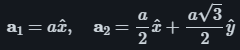
\includegraphics[max width=0.88\linewidth,max height=0.62\textheight,keepaspectratio]{assets/figure-b34c312a7a8e.png}
\end{figure}\par\par


为简化计算,取晶格常数a=1。轨道位置用约化坐标表示为:\par


\par\begin{figure}[H]\centering
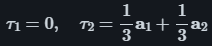
\includegraphics[max width=0.88\linewidth,max height=0.62\textheight,keepaspectratio]{assets/figure-724d1435aaff.png}
\end{figure}\par\par


此设定对应类似石墨烯的结构。通过Lattice类封装晶格几何信息,可实现晶格定义与模型构建的分离,提升代码的清晰度和可维护性。\par


\begin{inlinecodebox}{短代码 · python}
\VerbatimInput[fontsize=\small,breaklines=true,breakanywhere=true,tabsize=2,listparameters={\setlength{\topsep}{0pt}\setlength{\partopsep}{0pt}\setlength{\parsep}{0pt}}]{code/031-003.py}
\end{inlinecodebox}


我们将上述信息传入类中以创建一个晶格对象。此外,我们还需指定哪些方向具有周期性。在本示例中,两个方向均被设为周期性。\par


\begin{inlinecodebox}{短代码 · python}
\VerbatimInput[fontsize=\small,breaklines=true,breakanywhere=true,tabsize=2,listparameters={\setlength{\topsep}{0pt}\setlength{\partopsep}{0pt}\setlength{\parsep}{0pt}}]{code/031-004.py}
\end{inlinecodebox}


我们可以通过打印晶格对象,查看其生成的报告,以验证其中封装的晶格属性是否与预期一致。\par


\begin{codeindexbox}{代码清单 A.31.5}
语言：python；完整代码见附录第 \pageref{code:31:5} 页，共 26 行。
\end{codeindexbox}


如果我们想获取轨道在笛卡尔坐标系中的位置,可以使用 Lattice类的 get\_\allowbreak{}orb\_\allowbreak{}vecs方法,并将其参数 cartesian设置为 True。\par


\begin{codeindexbox}{代码清单 A.31.6}
语言：python；完整代码见附录第 \pageref{code:31:6} 页，共 1 行。
\end{codeindexbox}


\begin{codeindexbox}{代码清单 A.31.7}
语言：python；完整代码见附录第 \pageref{code:31:7} 页，共 2 行。
\end{codeindexbox}


该类内部会根据提供的晶格矢量和周期性生成倒格矢。我们可以通过 Lattice类的方法 get\_\allowbreak{}recip\_\allowbreak{}lat\_\allowbreak{}vecs或属性 recip\_\allowbreak{}lat\_\allowbreak{}vecs来访问这些倒格矢。\par


\begin{codeindexbox}{代码清单 A.31.8}
语言：python；完整代码见附录第 \pageref{code:31:8} 页，共 2 行。
\end{codeindexbox}


\begin{codeindexbox}{代码清单 A.31.9}
语言：python；完整代码见附录第 \pageref{code:31:9} 页，共 4 行。
\end{codeindexbox}


让我们验证倒格矢是否满足与实空间晶格矢量的正交性条件。\par


\par\begin{figure}[H]\centering

\includegraphics[max width=0.88\linewidth,max height=0.62\textheight,keepaspectratio]{assets/figure-bcfd10796ea6.png}
\end{figure}\par\par


\begin{inlinecodebox}{短代码 · python}
\VerbatimInput[fontsize=\small,breaklines=true,breakanywhere=true,tabsize=2,listparameters={\setlength{\topsep}{0pt}\setlength{\partopsep}{0pt}\setlength{\parsep}{0pt}}]{code/031-010.py}
\end{inlinecodebox}


\begin{codeindexbox}{代码清单 A.31.11}
语言：python；完整代码见附录第 \pageref{code:31:11} 页，共 2 行。
\end{codeindexbox}


如果需要,我们也可以获取实空间和倒空间中的原胞体积,这些值存储在 Lattice类的相应属性中。\par


\begin{codeindexbox}{代码清单 A.31.12}
语言：python；完整代码见附录第 \pageref{code:31:12} 页，共 1 行。
\end{codeindexbox}


\begin{codeindexbox}{代码清单 A.31.13}
语言：python；完整代码见附录第 \pageref{code:31:13} 页，共 1 行。
\end{codeindexbox}


完整代码如下:\par


\begin{codeindexbox}{代码清单 A.31.14}
语言：python；完整代码见附录第 \pageref{code:31:14} 页，共 90 行。
\end{codeindexbox}



\section{pythTB的学习\_\allowbreak{}mesh类}
\begin{articlemeta}
\textbf{日期：}2025-12-09\hfill\textbf{在线原文：}\href{https://marx2001.github.io/sci-note\_posts/20251209-PythonTB\_mesh}{marx2001.github.io}
\end{articlemeta}

\subsection{Tutorials}


本教程将演示如何在组合布里渊区(BZ)与参数空间中创建自定义网格与环绕路径。\par


\begin{codeindexbox}{代码清单 A.32.1}
语言：python；完整代码见附录第 \pageref{code:32:1} 页，共 2 行。
\end{codeindexbox}


Mesh对象接受以下参数:\par


•axis\_\allowbreak{}types:字符串列表,定义每个坐标轴的类型。选项为 “k”(晶格动量,约化单位)和 “l”(绝热参数)。\par


•axis\_\allowbreak{}names(可选):字符串列表,定义每个坐标轴的名称,主要用于绝热循环(示例可见“三格点 Thouless 泵”案例)。\par


•dim\_\allowbreak{}k(可选):整数,定义 k 空间的维度。当 “k”轴的数量少于 dim\_\allowbreak{}k时(例如在二维布里渊区中沿一维路径采样)必须提供此参数。\par


在下面的代码单元中,我们将在二维k空间中创建一个仅包含单个k轴的网格。这意味着该网格是二维布里渊区(BZ)中的一条路径。我们将使用 build\_\allowbreak{}custom()方法直接指定网格点。这里我们创建了一条从 Γ 点 [0, 0] 经过 X点 [0.5, 0.5] 到下一个单元中的 Γ点 [1, 1] 的路径。\par


\begin{codeindexbox}{代码清单 A.32.2}
语言：python；完整代码见附录第 \pageref{code:32:2} 页，共 5 行。
\end{codeindexbox}


我们可以通过 points属性访问网格点。请注意,网格中的每个点都是一个二维向量,对应于两个 k 空间维度。\par


\begin{codeindexbox}{代码清单 A.32.3}
语言：python；完整代码见附录第 \pageref{code:32:3} 页，共 3 行。
\end{codeindexbox}


结果:\par


\begin{codeindexbox}{代码清单 A.32.4}
语言：python；完整代码见附录第 \pageref{code:32:4} 页，共 12 行。
\end{codeindexbox}


我们可以通过打印对象来查看网格信息。这会告诉我们:\par


网格类型(”path” 路径 或 “grid” 网格)\par


k空间和参数空间的维度数\par


网格点的总数\par


网格数组的形状\par


k轴(类型(k)、名称、点数)\par


参数空间轴(类型(l)、名称、点数)\par


哪些轴是循环(周期性)的,哪些不是\par


网格中存在的环(若有)\par


\begin{codeindexbox}{代码清单 A.32.5}
语言：python；完整代码见附录第 \pageref{code:32:5} 页，共 1 行。
\end{codeindexbox}


\begin{codeindexbox}{代码清单 A.32.6}
语言：python；完整代码见附录第 \pageref{code:32:6} 页，共 9 行。
\end{codeindexbox}


代码本身无法自动判断在端点未包含时,哪些轴应对布里渊区(BZ)或参数空间进行“卷绕”,因此需要手动指定。这对于正确布洛赫波函数的周期性边界条件非常重要。\par


可以通过调用 loop 方法来声明一个轴对布里渊区进行卷绕。该方法接受以下参数:\par


axis\_\allowbreak{}idx:要卷绕的轴索引(从0开始计数)。\par


component\_\allowbreak{}idx:在组合的 (k, λ) 向量中对应的分量索引(从0开始计数)。\par


winds\_\allowbreak{}bz:布尔值,指示该轴是否通过倒格矢卷绕布里渊区(True表示是)。\par


closed:布尔值,指示该轴是否包含端点(即是否为闭合的轴)(False表示不包含)。\par


在该示例中,设置了:\par


将网格的第一个(且唯一一个)轴 (axis\_\allowbreak{}idx=0) 设置为卷绕第一个k空间维度 (component\_\allowbreak{}idx=0),调用 loop(axis\_\allowbreak{}idx=0, component\_\allowbreak{}idx=0, winds\_\allowbreak{}bz=True, closed=False)。\par


为了也对第二个k空间维度进行卷绕,再次调用 loop方法,但这次设置 component\_\allowbreak{}idx=1(即 axis\_\allowbreak{}idx=0, component\_\allowbreak{}idx=1, winds\_\allowbreak{}bz=True, closed=False))。\par


调用完成后,网格信息将显示两个轴均绕布里渊区卷绕。\par


注意:\par


当使用k点时,应通过设置 winds\_\allowbreak{}bz参数来明确该轴是否绕布里渊区(BZ)倒格矢一周。这确保了布洛赫波函数在周期性边界条件下得到正确处理。\par


若该轴绕布里渊区一周(例如跨越整个布里渊区的高对称路径),应设置为 winds\_\allowbreak{}bz=True。\par


若该轴不环绕布里渊区(例如布里渊区内部的小环形路径,如狄拉克点周围的闭合环路),则应设置为 winds\_\allowbreak{}bz=False。\par


此设置对确保波函数相位和拓扑计算的正确性至关重要。\par


\begin{codeindexbox}{代码清单 A.32.7}
语言：python；完整代码见附录第 \pageref{code:32:7} 页，共 6 行。
\end{codeindexbox}


\begin{codeindexbox}{代码清单 A.32.8}
语言：python；完整代码见附录第 \pageref{code:32:8} 页，共 9 行。
\end{codeindexbox}


我们将进行与之前相同的操作,但这次会将布里渊区(BZ)的端点包含在内。\par


注意:\par


Mesh类具备自动检测功能:如果 k 分量的起点和终点在模 1 下相等(即该轴是闭合的),则会自动将该轴识别为环绕布里渊区。因此,即使在以 Γ 点为中心(k 分量范围在 [-0.5, 0.5] 内)的网格中,如果包含了端点(±0.5),该类仍可检测到该轴环绕布里渊区。\par


\begin{codeindexbox}{代码清单 A.32.9}
语言：python；完整代码见附录第 \pageref{code:32:9} 页，共 7 行。
\end{codeindexbox}


\begin{codeindexbox}{代码清单 A.32.10}
语言：python；完整代码见附录第 \pageref{code:32:10} 页，共 9 行。
\end{codeindexbox}



\section{pythTB的学习\_\allowbreak{}tb\_\allowbreak{}model to TBModel in v2.0}
\begin{articlemeta}
\textbf{日期：}2025-12-09\hfill\textbf{在线原文：}\href{https://marx2001.github.io/sci-note\_posts/20251209-PythonTB\_tb}{marx2001.github.io}
\end{articlemeta}

\subsection{Tutorials}


在 TBModel 类的 v2.0 版本中,模块名称已发生重要变更。v1.8 版本中的 tb\_\allowbreak{}model、wf\_\allowbreak{}array和 w90在 v2.0 版本中已分别更新为 TBModel、WFArray 和 W90。在使用时,请注意在代码的导入行中相应 修改模块名称。\par


\begin{codeindexbox}{代码清单 A.33.1}
语言：python；完整代码见附录第 \pageref{code:33:1} 页，共 2 行。
\end{codeindexbox}


\subsubsection{构建一个TB模型}


在 v2.0 版本中,模型的构建方式发生了变化。我们不再将晶格矢量和轨道位置作为单独的参数传递,而是传递一个包含这些信息的 Lattice对象。\par


我们将以蜂窝晶格为例进行说明。在 v1.8 版本中,我们会这样操作:\par


\begin{codeindexbox}{代码清单 A.33.2}
语言：python；完整代码见附录第 \pageref{code:33:2} 页，共 6 行。
\end{codeindexbox}


在 v2.0 版本中,我们首先创建一个 Lattice对象,然后将其传递给 TBModel构造器。\par


需要注意的几个行为变化如下:\par


为提高清晰度,per参数已更名为 periodic\_\allowbreak{}dirs。若未指定,v1.8 版本的默认行为是假设所有方向均为周期性的;而在 v2.0 中,默认设置为无周期性方向。\par


整数参数 nspin已被替换为布尔型参数 spinful,用于指示模型是否具有自旋自由度。\par


dim\_\allowbreak{}r和 dim\_\allowbreak{}k不再是必需参数,因为它们可以从 lat\_\allowbreak{}vecs和 periodic\_\allowbreak{}dirs中推断得出。\par


其余大部分功能基本保持不变,仅被封装在 Lattice对象中。\par


\#\#\#\#提示:\par


将所有晶格方向指定为周期性的便捷方法是为 periodic\_\allowbreak{}dirs参数使用 ...,例如 periodic\_\allowbreak{}dirs=...。此外,也可以通过传递 periodic\_\allowbreak{}dirs=”all”来实现相同效果。\par


以下是 v2.0 中对应的代码:\par


\begin{inlinecodebox}{短代码 · python}
\VerbatimInput[fontsize=\small,breaklines=true,breakanywhere=true,tabsize=2,listparameters={\setlength{\topsep}{0pt}\setlength{\partopsep}{0pt}\setlength{\parsep}{0pt}}]{code/033-003.py}
\end{inlinecodebox}


\begin{codeindexbox}{代码清单 A.33.4}
语言：python；完整代码见附录第 \pageref{code:33:4} 页，共 14 行。
\end{codeindexbox}


\subsubsection{模型库}


一系列用于原型紧束缚模型的 TBModel 生成器已被收录在 pythtb.models中。这些模型包括:\par


棋盘模型\par


霍尔丹模型\par


凯恩-梅莱模型\par


石墨烯模型\par


举个例子,我们可以从模型库中导入与上文相同的霍尔丹紧束缚模型:\par


\begin{codeindexbox}{代码清单 A.33.5}
语言：python；完整代码见附录第 \pageref{code:33:5} 页，共 3 行。
\end{codeindexbox}


\subsubsection{报告模型信息}


使用下面代码查看模型信息:\par


\begin{codeindexbox}{代码清单 A.33.6}
语言：python；完整代码见附录第 \pageref{code:33:6} 页，共 7 行。
\end{codeindexbox}


\begin{codeindexbox}{代码清单 A.33.7}
语言：python；完整代码见附录第 \pageref{code:33:7} 页，共 1 行。
\end{codeindexbox}


结果:\par


\begin{codeindexbox}{代码清单 A.33.8}
语言：python；完整代码见附录第 \pageref{code:33:8} 页，共 52 行。
\end{codeindexbox}


\subsubsection{紧束缚模型的可视化}


紧束缚模型(TB)的轨道位置与跃迁键的可视化功能已更新。\par


与之前一样,我们调用 my\_\allowbreak{}model.visualize来查看紧束缚晶格。\par


在 v1.8 版本中,应使用如下方式:\par


\begin{codeindexbox}{代码清单 A.33.9}
语言：python；完整代码见附录第 \pageref{code:33:9} 页，共 2 行。
\end{codeindexbox}


结果图为: 
\par\begin{figure}[H]\centering
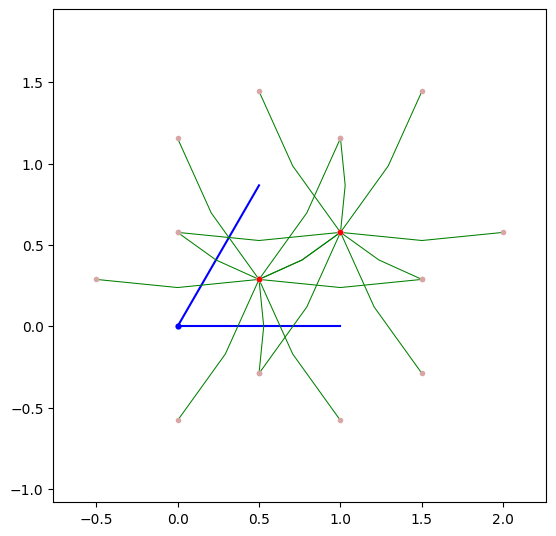
\includegraphics[max width=0.88\linewidth,max height=0.62\textheight,keepaspectratio]{assets/figure-79c83298d674.png}
\end{figure}\par\par


区别在于,在绘制二维图形时,我们不再需要指定晶格方向。对于三维模型,仍可通过 proj\_\allowbreak{}plane参数指定两个对应于ai和aj晶格矢量的整数,以将三维结构投影到该平面上。默认行为是:二维模型直接绘制二 维图形,三维模型默认投影到 a1-a2平面上。..note:: 对于三维模型,如果安装了 plotly,现在可以使用 visualize3d()绘制三维结构。\par


在 v2.0 版本中,输出效果如下所示:\par


\par\begin{figure}[H]\centering
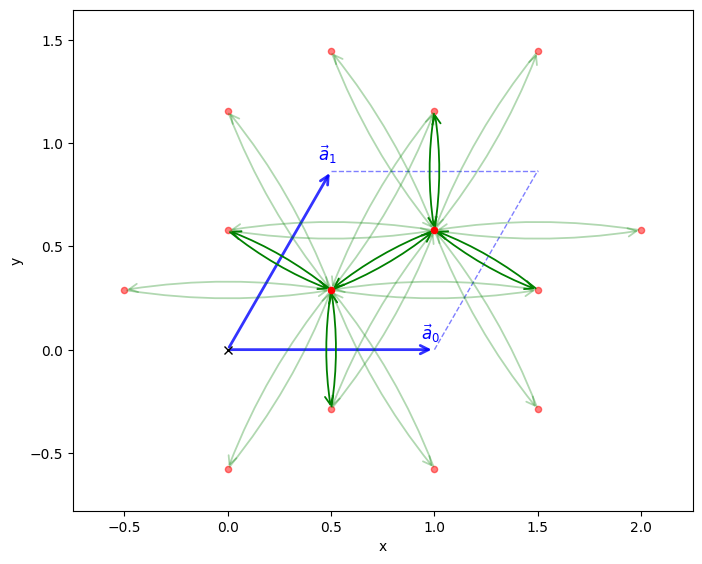
\includegraphics[max width=0.88\linewidth,max height=0.62\textheight,keepaspectratio]{assets/figure-ddea0d20603c.png}
\end{figure}\par\par


请注意,图中键的粗细并非完全一致。其透明度(alpha 值)会根据跃迁强度进行比例缩放。此外,我们现在还可以通过设置 annotate\_\allowbreak{}onsite\_\allowbreak{}en参数为 True来标注每个格点的位能值。\par


\subsubsection{获得哈密顿量矩阵}


在pythtb的旧版本中,用户无法直接获取哈密顿矩阵。相反,需要通过调用my\_\allowbreak{}model.solve\_\allowbreak{}all(kpts)或my\_\allowbreak{}model.solve\_\allowbreak{}one(kpt)函数来获取给定k点的本征值和本征向量。而在v2.0版本中,新增了 my\_\allowbreak{}model.hamiltonian(kpts)方法,允许用户直接获取一系列k点上的哈密顿矩阵,该方法会返回一个NumPy数组。\par


\begin{codeindexbox}{代码清单 A.33.10}
语言：python；完整代码见附录第 \pageref{code:33:10} 页，共 3 行。
\end{codeindexbox}


\begin{inlinecodebox}{短代码 · python}
\VerbatimInput[fontsize=\small,breaklines=true,breakanywhere=true,tabsize=2,listparameters={\setlength{\topsep}{0pt}\setlength{\partopsep}{0pt}\setlength{\parsep}{0pt}}]{code/033-011.py}
\end{inlinecodebox}


\begin{codeindexbox}{代码清单 A.33.12}
语言：python；完整代码见附录第 \pageref{code:33:12} 页，共 7 行。
\end{codeindexbox}


\subsubsection{能带绘制}


TBModel 的一个新功能是增加了一个便捷函数,可快速绘制能带结构。我们不再需要显式创建 k 路径和 matplotlib 图形,只需调用 plot\_\allowbreak{}bands 并传递以约化单位表示的高对称点即可。这将返回 matplotlib 图形和坐标轴对象,以供进一步自定义。\par


注意\par


我们还可以传递 k\_\allowbreak{}node\_\allowbreak{}labels 参数来指定高对称点的标签。\par


\begin{codeindexbox}{代码清单 A.33.13}
语言：python；完整代码见附录第 \pageref{code:33:13} 页，共 17 行。
\end{codeindexbox}


\begin{inlinecodebox}{短代码 · python}
\VerbatimInput[fontsize=\small,breaklines=true,breakanywhere=true,tabsize=2,listparameters={\setlength{\topsep}{0pt}\setlength{\partopsep}{0pt}\setlength{\parsep}{0pt}}]{code/033-014.py}
\end{inlinecodebox}


一个可选参数允许用户可视化能带的轨道特征。为此,我们向 proj\_\allowbreak{}orb\_\allowbreak{}idx参数提供一个列表。该列表定义了用于本征态投影的轨道索引。系统将显示一个颜色条,展示本征态在这些轨道集合上的权重。\par


在本示例中,Haldane 模型在 K 点和 K’ 点处展示了能带反转现象,这正是拓扑相变的典型特征。\par


\begin{codeindexbox}{代码清单 A.33.15}
语言：python；完整代码见附录第 \pageref{code:33:15} 页，共 3 行。
\end{codeindexbox}


\par\begin{figure}[H]\centering
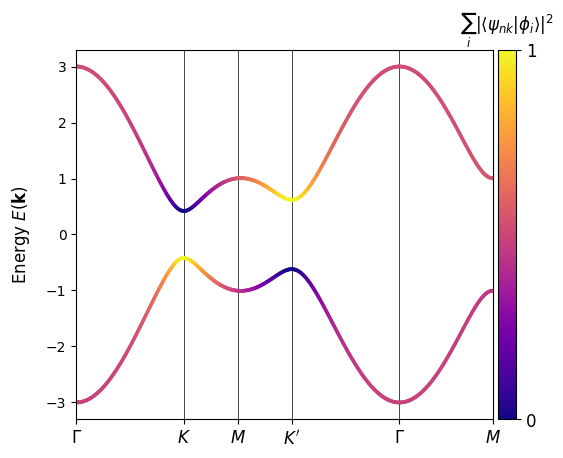
\includegraphics[max width=0.88\linewidth,max height=0.62\textheight,keepaspectratio]{assets/figure-392b9eed7e60.png}
\end{figure}\par\par


\subsubsection{向后兼容性}


为保持与为 PythTB v1.8 及更早版本编写的脚本的向后兼容性,旧版 tb\_\allowbreak{}model仍可作为 TBModel的别名使用。其函数与方法将采用 v2.0 版本的实现,但初始化 tb\_\allowbreak{}model类的旧方式依然有效。\par


\begin{codeindexbox}{代码清单 A.33.16}
语言：python；完整代码见附录第 \pageref{code:33:16} 页，共 2 行。
\end{codeindexbox}


从V1.8.0的Haldane model initialization:\par


\begin{codeindexbox}{代码清单 A.33.17}
语言：python；完整代码见附录第 \pageref{code:33:17} 页，共 31 行。
\end{codeindexbox}


\begin{codeindexbox}{代码清单 A.33.18}
语言：python；完整代码见附录第 \pageref{code:33:18} 页，共 52 行。
\end{codeindexbox}


\begin{codeindexbox}{代码清单 A.33.19}
语言：python；完整代码见附录第 \pageref{code:33:19} 页，共 4 行。
\end{codeindexbox}



\section{pythTB的学习\_\allowbreak{}wf\_\allowbreak{}array to in v2.0WFArray}
\begin{articlemeta}
\textbf{日期：}2025-12-09\hfill\textbf{在线原文：}\href{https://marx2001.github.io/sci-note\_posts/20251209-PythonTB\_tb2}{marx2001.github.io}
\end{articlemeta}

\subsection{Tutorials}


\subsubsection{初始化与填充 WFArray}


在 PythTB 的旧版本中,wf\_\allowbreak{}array类与 tb\_\allowbreak{}model类紧密耦合。初始化 wf\_\allowbreak{}array时,它会从关联的 tb\_\allowbreak{}model中读取晶格信息。而在 v2.0 版本中,与 TBModel的做法类似,我们将显式地将一个 Lattice对 象传递给 WFArray的构造函数。除了提高灵活性,这也使我们能够创建不绑定于任何特定 TBModel的 WFArray对象。例如,用户可能希望存储源自绝热循环中多个 TBModel的状态,而这些状态没有一个单一的 TBModel可以完全描述。\par


Compare to versions 1.x:\par


\begin{codeindexbox}{代码清单 A.34.1}
语言：python；完整代码见附录第 \pageref{code:34:1} 页，共 5 行。
\end{codeindexbox}


在 solve\_\allowbreak{}on\_\allowbreak{}grid方法中,wf\_\allowbreak{}array会先生成 k 点网格,并用来自 model的波函数数据填充自身。之后,这个 k 点网格会被丢弃,wf\_\allowbreak{}array仅保留波函数数据本身。这导致关于 k 点结构的信息丢失,如果后续分析(如绘图)需要这些 k 点信息,用户需要自己手动追踪和保存对应的 k 点网格。\par


\begin{enumerate}
\item 创建一个描述系统晶格结构的对象。
\end{enumerate}


\begin{inlinecodebox}{短代码 · python}
\VerbatimInput[fontsize=\small,breaklines=true,breakanywhere=true,tabsize=2,listparameters={\setlength{\topsep}{0pt}\setlength{\partopsep}{0pt}\setlength{\parsep}{0pt}}]{code/034-002.py}
\end{inlinecodebox}


\begin{enumerate}
\item 创建一个用于描述k点和参数网格的对象。
\end{enumerate}


\begin{inlinecodebox}{短代码 · python}
\VerbatimInput[fontsize=\small,breaklines=true,breakanywhere=true,tabsize=2,listparameters={\setlength{\topsep}{0pt}\setlength{\partopsep}{0pt}\setlength{\parsep}{0pt}}]{code/034-003.py}
\end{inlinecodebox}


\begin{enumerate}
\item 用所需的k点和参数值填充Mesh。
\end{enumerate}


\begin{codeindexbox}{代码清单 A.34.4}
语言：python；完整代码见附录第 \pageref{code:34:4} 页，共 1 行。
\end{codeindexbox}


\begin{enumerate}
\item 将这些对象传递给构造函数
\end{enumerate}


\begin{inlinecodebox}{短代码 · python}
\VerbatimInput[fontsize=\small,breaklines=true,breakanywhere=true,tabsize=2,listparameters={\setlength{\topsep}{0pt}\setlength{\partopsep}{0pt}\setlength{\parsep}{0pt}}]{code/034-005.py}
\end{inlinecodebox}


现在,如果我们想用一个给定的 TBModel的能量本征态来填充 WFArray,可以通过调用 WFArray.solve\_\allowbreak{}model()函数来实现。\par


\begin{codeindexbox}{代码清单 A.34.6}
语言：python；完整代码见附录第 \pageref{code:34:6} 页，共 18 行。
\end{codeindexbox}


\begin{inlinecodebox}{短代码 · python}
\VerbatimInput[fontsize=\small,breaklines=true,breakanywhere=true,tabsize=2,listparameters={\setlength{\topsep}{0pt}\setlength{\partopsep}{0pt}\setlength{\parsep}{0pt}}]{code/034-007.py}
\end{inlinecodebox}


我们可以通过索引来访问存储在 WFArray中的单个波函数,这与先前版本中的操作方式相似。例如,wfa[k\_\allowbreak{}index]将返回指定网格索引处的波函数。\par


\begin{codeindexbox}{代码清单 A.34.8}
语言：python；完整代码见附录第 \pageref{code:34:8} 页，共 1 行。
\end{codeindexbox}


\begin{codeindexbox}{代码清单 A.34.9}
语言：python；完整代码见附录第 \pageref{code:34:9} 页，共 6 行。
\end{codeindexbox}


与先前版本一样,在贝里相位计算及其他运算中,布里渊区边界会自动应用内部的周期性边界条件。\par


\subsubsection{绝热循环中的 WFArray}


我们将复用上文使用过的同一个晶格,但现在要创建一个包含绝热参数轴的 Mesh。这个参数在 0 到 1 的范围内变化,共分 11 个步骤。这个参数可以代表例如晶格的畸变或外部场的变化。\par


Mesh lambda 01\par


可回顾 Mesh 教程中的内容:我们需要根据在函数中变化的参数名称来命名这个坐标轴(如未阅读,可参阅上文的函数说明)。\par


λ TBModel1\par


\begin{inlinecodebox}{短代码 · python}
\VerbatimInput[fontsize=\small,breaklines=true,breakanywhere=true,tabsize=2,listparameters={\setlength{\topsep}{0pt}\setlength{\partopsep}{0pt}\setlength{\parsep}{0pt}}]{code/034-010.py}
\end{inlinecodebox}


现在我们将构建网格,指定绝热参数的范围从0到1,共分11个步骤。\par


\begin{codeindexbox}{代码清单 A.34.11}
语言：python；完整代码见附录第 \pageref{code:34:11} 页，共 7 行。
\end{codeindexbox}


如果我们希望将 λ 轴设置为一个绝热循环,我们需要为对应的轴索引设置 loop 参数。组合空间(k, λ)是二维的,且维度排列在 k 维度(这里只有 1 个 k 维度)之后,因此组件索引是 1(按 Python 计 数方式)。这表明,遍历轴 1 会使网格向量的第二个分量(Python 计数为 1)形成环路,从而使得环路末端的哈密顿量与起始端的哈密顿量相连。\par


由于 λ=1 的终点与 λ=0 的起点是等效的,我们也将该轴标记为闭合。这可以通过将 closed 参数设置为 True 来实现。\par


\begin{codeindexbox}{代码清单 A.34.12}
语言：python；完整代码见附录第 \pageref{code:34:12} 页，共 4 行。
\end{codeindexbox}


\begin{codeindexbox}{代码清单 A.34.13}
语言：python；完整代码见附录第 \pageref{code:34:13} 页，共 10 行。
\end{codeindexbox}


初始化WFArray\par


\begin{inlinecodebox}{短代码 · python}
\VerbatimInput[fontsize=\small,breaklines=true,breakanywhere=true,tabsize=2,listparameters={\setlength{\topsep}{0pt}\setlength{\partopsep}{0pt}\setlength{\parsep}{0pt}}]{code/034-014.py}
\end{inlinecodebox}


最后,我们调用函数,在组合网格的每个点 (k, λ) 上,用 TBModel 的本征态填充 WFAArray。\par


\begin{codeindexbox}{代码清单 A.34.15}
语言：python；完整代码见附录第 \pageref{code:34:15} 页，共 1 行。
\end{codeindexbox}


我们可以通过比较绝热循环开始和结束时的波函数,来验证该轴是否被正确设置为一个环路\par


\begin{codeindexbox}{代码清单 A.34.16}
语言：python；完整代码见附录第 \pageref{code:34:16} 页，共 1 行。
\end{codeindexbox}


\begin{codeindexbox}{代码清单 A.34.17}
语言：python；完整代码见附录第 \pageref{code:34:17} 页，共 1 行。
\end{codeindexbox}



\section{vasp2kp的学习\_\allowbreak{}1}
\begin{articlemeta}
\textbf{日期：}2025-12-10\hfill\textbf{在线原文：}\href{https://marx2001.github.io/sci-note\_posts/20251210-vasp2kp}{marx2001.github.io}
\end{articlemeta}

\subsection{Tutorials}


\subsubsection{初始化与填充 WFArray}


\par\begin{figure}[H]\centering
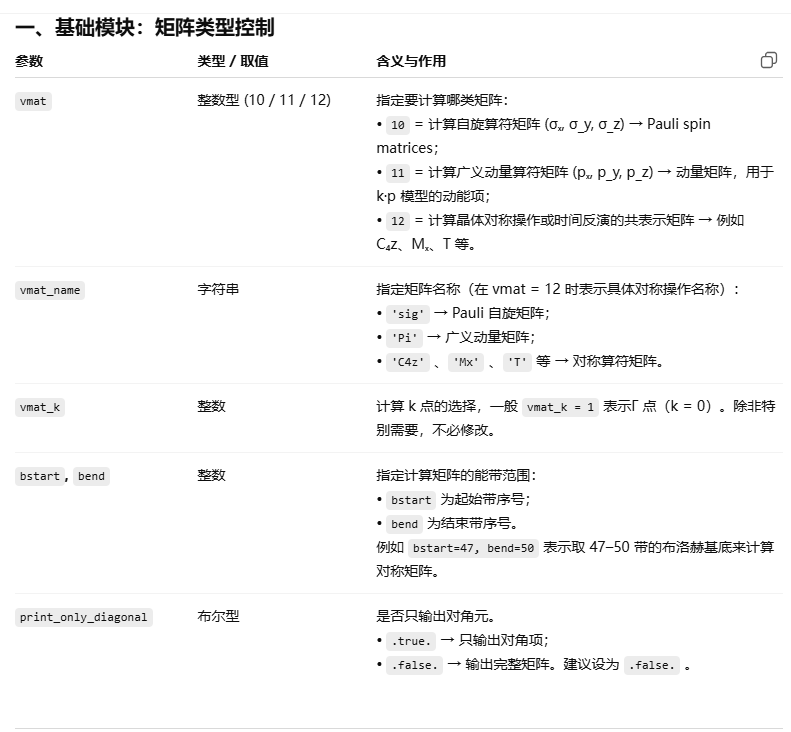
\includegraphics[max width=0.88\linewidth,max height=0.62\textheight,keepaspectratio]{assets/figure-aec29f9091a5.png}
\end{figure}\par\par


\par\begin{figure}[H]\centering
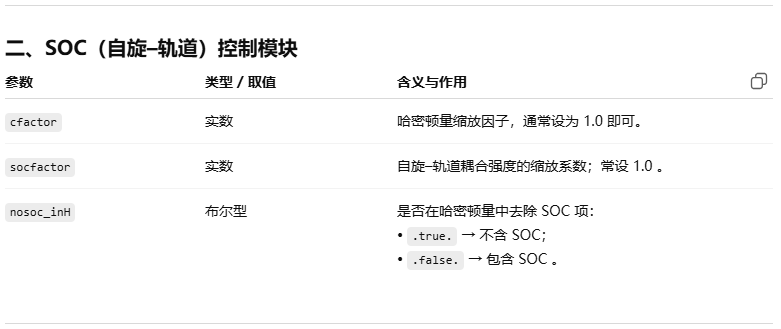
\includegraphics[max width=0.88\linewidth,max height=0.62\textheight,keepaspectratio]{assets/figure-7df2b4942a05.png}
\end{figure}\par\par


\par\begin{figure}[H]\centering
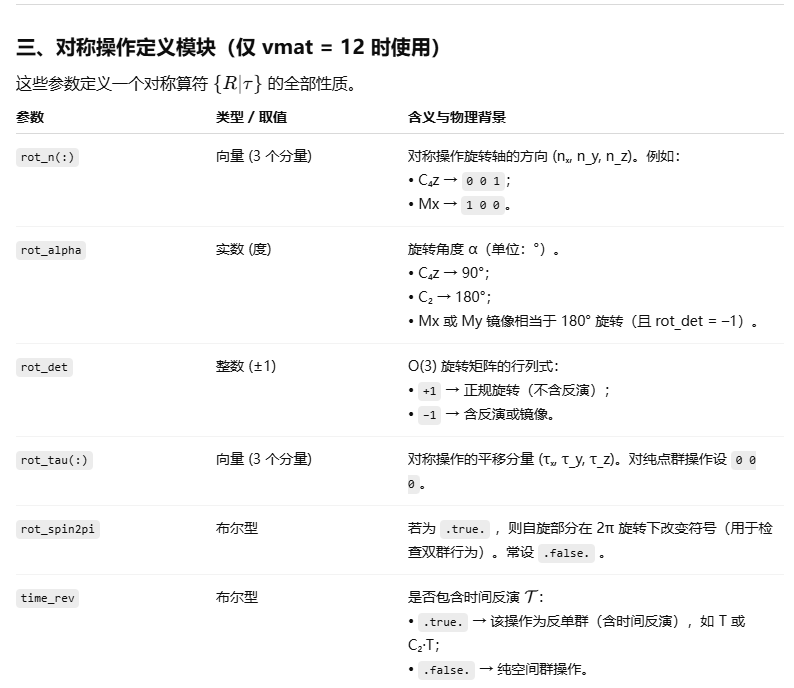
\includegraphics[max width=0.88\linewidth,max height=0.62\textheight,keepaspectratio]{assets/figure-2006c3913eeb.png}
\end{figure}\par\par


\par\begin{figure}[H]\centering
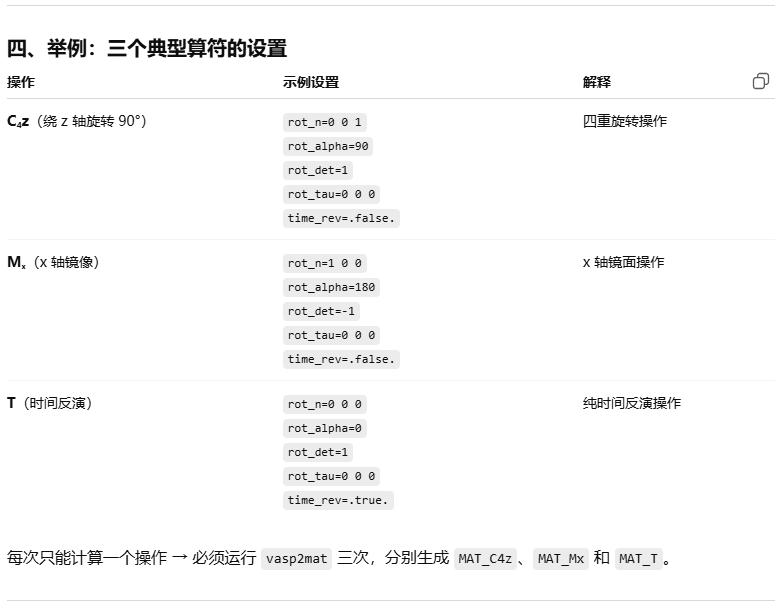
\includegraphics[max width=0.88\linewidth,max height=0.62\textheight,keepaspectratio]{assets/figure-14b50036bc6e.png}
\end{figure}\par\par


需要6个初始文件作为输入文件\par


\begin{codeindexbox}{代码清单 A.35.1}
语言：python；完整代码见附录第 \pageref{code:35:1} 页，共 1 行。
\end{codeindexbox}


运行命令开始计算:\par


\begin{inlinecodebox}{短代码 · python}
\VerbatimInput[fontsize=\small,breaklines=true,breakanywhere=true,tabsize=2,listparameters={\setlength{\topsep}{0pt}\setlength{\partopsep}{0pt}\setlength{\parsep}{0pt}}]{code/035-002.py}
\end{inlinecodebox}



\section{ir2TB的学习}
\begin{articlemeta}
\textbf{日期：}2025-12-13\hfill\textbf{在线原文：}\href{https://marx2001.github.io/sci-note\_posts/20251213-ir2TB}{marx2001.github.io}
\end{articlemeta}

\subsection{Tutorials}


\subsubsection{简介:Why is IRVSP\&IR2TB}


\par\begin{figure}[H]\centering
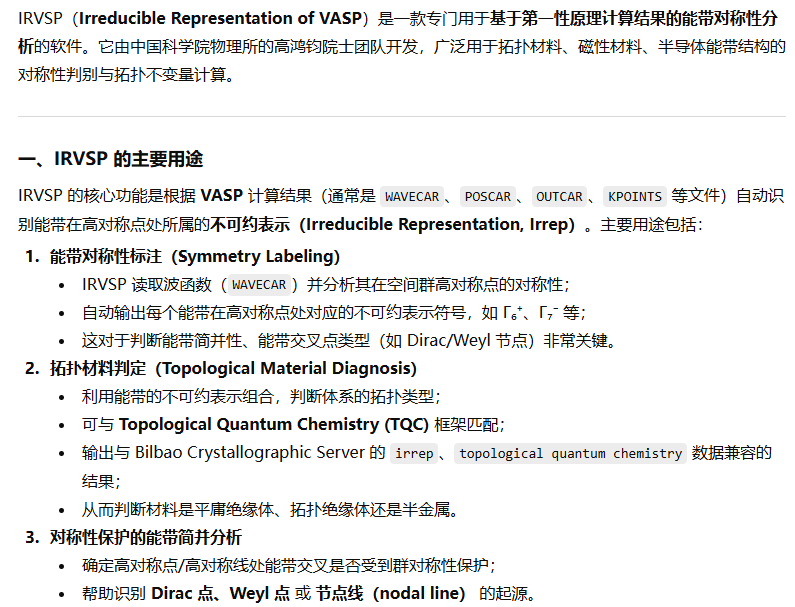
\includegraphics[max width=0.88\linewidth,max height=0.62\textheight,keepaspectratio]{assets/figure-af266d2fdadf.png}
\end{figure}\par\par


\par\begin{figure}[H]\centering
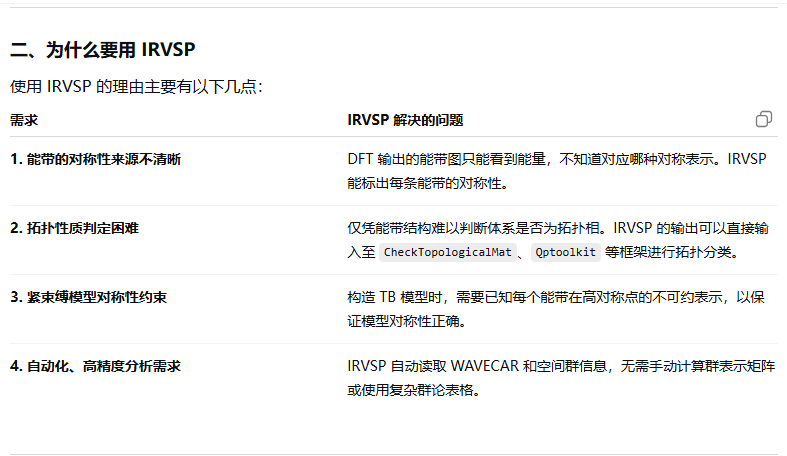
\includegraphics[max width=0.88\linewidth,max height=0.62\textheight,keepaspectratio]{assets/figure-ce32f52da1be.png}
\end{figure}\par\par


\par\begin{figure}[H]\centering

\includegraphics[max width=0.88\linewidth,max height=0.62\textheight,keepaspectratio]{assets/figure-a0aec7da843d.png}
\end{figure}\par\par


\subsection{IRVSP的使用}


用于判断非常规材料的电子性质(电子的电荷中心不在原子上),用拓扑量子化学和能带表示的理论,通过高对称k点的表示可以判断出来。(阻挫原子极限)\par


先确定能带的基本情况\par


\begin{enumerate}
\item 先找到POSCAR\par
\item 用phonopy跑一遍,得到标准化poscar。\par
\item 先算自洽,再算高对称k点的表示\par
\item 非自洽,算能带(kpoints需要特殊准备),chgcar不变,输出wavecar,得到高对称K点的波函数\par
\end{enumerate}


\begin{codeindexbox}{代码清单 A.36.1}
语言：shell；完整代码见附录第 \pageref{code:36:1} 页，共 1 行。
\end{codeindexbox}


看对应的能带表示\par


\begin{codeindexbox}{代码清单 A.36.2}
语言：shell；完整代码见附录第 \pageref{code:36:2} 页，共 1 行。
\end{codeindexbox}


看tqc.data、EBR等等。\par


见吴泉生老师的官网和B站视频均有资源,此为简单记录一些命令,方便复制命令。\par



\section{irvsp的学习}
\begin{articlemeta}
\textbf{日期：}2025-12-13\hfill\textbf{在线原文：}\href{https://marx2001.github.io/sci-note\_posts/20251213-irvsp}{marx2001.github.io}
\end{articlemeta}

\subsection{Tutorials}


\subsubsection{简介:Why is IRVSP\&IR2TB}


\par\begin{figure}[H]\centering
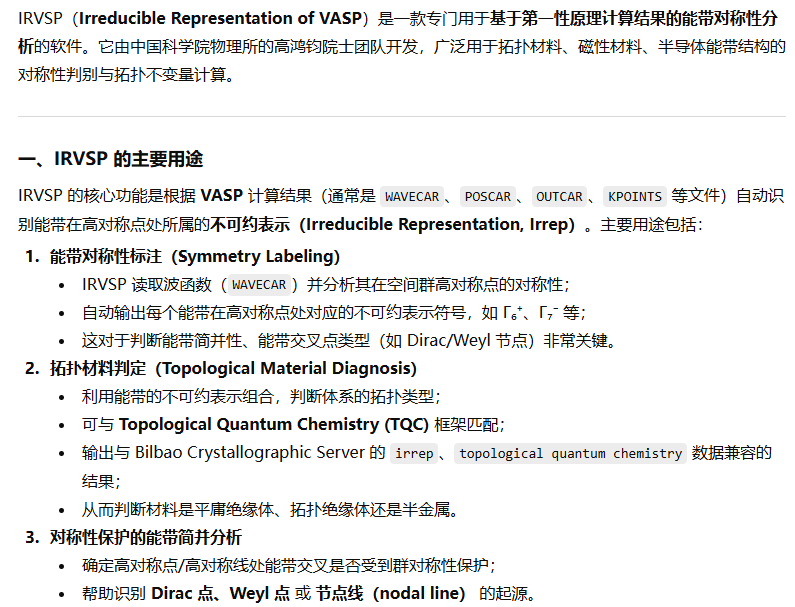
\includegraphics[max width=0.88\linewidth,max height=0.62\textheight,keepaspectratio]{assets/figure-af266d2fdadf.png}
\end{figure}\par\par


\par\begin{figure}[H]\centering
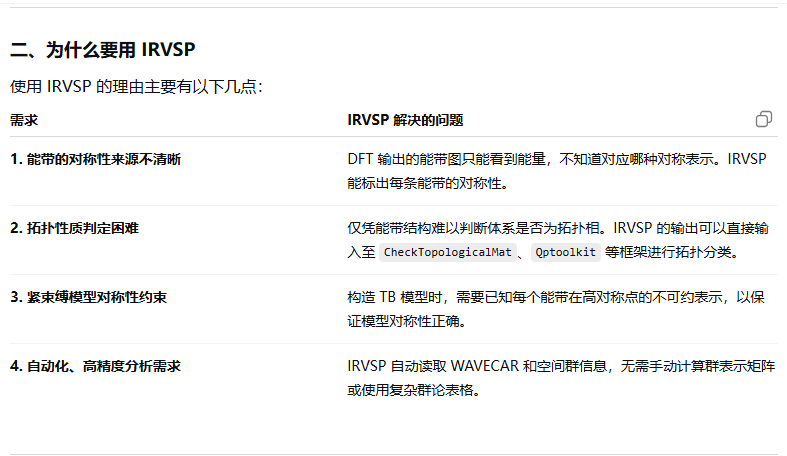
\includegraphics[max width=0.88\linewidth,max height=0.62\textheight,keepaspectratio]{assets/figure-ce32f52da1be.png}
\end{figure}\par\par


\par\begin{figure}[H]\centering

\includegraphics[max width=0.88\linewidth,max height=0.62\textheight,keepaspectratio]{assets/figure-a0aec7da843d.png}
\end{figure}\par\par


\subsection{IRVSP的使用}


用于判断非常规材料的电子性质(电子的电荷中心不在原子上),用拓扑量子化学和能带表示的理论,通过高对称k点的表示可以判断出来。(阻挫原子极限)\par


先确定能带的基本情况\par


\begin{enumerate}
\item 先找到POSCAR\par
\item 用phonopy跑一遍,得到标准化poscar。\par
\item 先算自洽,再算高对称k点的表示\par
\item 非自洽,算能带(kpoints需要特殊准备),chgcar不变,输出wavecar,得到高对称K点的波函数\par
\end{enumerate}


\begin{codeindexbox}{代码清单 A.37.1}
语言：shell；完整代码见附录第 \pageref{code:37:1} 页，共 1 行。
\end{codeindexbox}


看对应的能带表示\par


\begin{codeindexbox}{代码清单 A.37.2}
语言：shell；完整代码见附录第 \pageref{code:37:2} 页，共 1 行。
\end{codeindexbox}


看tqc.data、EBR等等。\par


13和13是能带序号\par



\section{(原创脚本)角态验证1-配置pybinding环境-Ubuntu系统配置}
\begin{articlemeta}
\textbf{日期：}2025-12-27\hfill\textbf{在线原文：}\href{https://marx2001.github.io/sci-note\_posts/20251227-pybinding}{marx2001.github.io}
\end{articlemeta}

\subsubsection{步骤}


windows环境下,需要下载cmake,和Visual Studio Build Tools:\par


\begin{codeindexbox}{代码清单 A.38.1}
语言：shell；完整代码见附录第 \pageref{code:38:1} 页，共 2 行。
\end{codeindexbox}


勾选:\par


\begin{codeindexbox}{代码清单 A.38.2}
语言：shell；完整代码见附录第 \pageref{code:38:2} 页，共 7 行。
\end{codeindexbox}


创建环境\par


\begin{inlinecodebox}{命令示例 · shell}
\VerbatimInput[fontsize=\small,breaklines=true,breakanywhere=true,tabsize=2,listparameters={\setlength{\topsep}{0pt}\setlength{\partopsep}{0pt}\setlength{\parsep}{0pt}}]{code/038-003.sh}
\end{inlinecodebox}


安装miniconda后,运行\par


\begin{inlinecodebox}{命令示例 · shell}
\VerbatimInput[fontsize=\small,breaklines=true,breakanywhere=true,tabsize=2,listparameters={\setlength{\topsep}{0pt}\setlength{\partopsep}{0pt}\setlength{\parsep}{0pt}}]{code/038-004.sh}
\end{inlinecodebox}


然后\par


\begin{inlinecodebox}{命令示例 · shell}
\VerbatimInput[fontsize=\small,breaklines=true,breakanywhere=true,tabsize=2,listparameters={\setlength{\topsep}{0pt}\setlength{\partopsep}{0pt}\setlength{\parsep}{0pt}}]{code/038-005.sh}
\end{inlinecodebox}


安装了Cmake和visual Studio installer仍然不能成功安装pybinding,尝试使用Linux环境,安装Ubantu\par


\subsubsection{安装Ubantu}


使用DiskGenius V4.6.4.2 x64专业版 ,选择有空余空间的磁盘,拖动棕色进度条,留出合适的空间。\par


使用Rufus 4.7.2231,写入Ubuntu镜像文件到安装u盘中,U盘要求16G以上。\par


12.28 用ubuntu系统成功安装了pybinding,用conda安装,先创建环境,然后用conda安装前置库,然后再安装pybinding。\par


在ubuntu中也不能直接用pip安装pybinding,只能用conda 安装0.9.5稳定版的pybinding。\par


安装完pybinding之后,由于是ipynb格式,需要jupyter notebook使用的kernel与安装的pybinding环境一致,这样代码才能在该环境中找到所需要的包并运行。\par


先激活环境,然后安装ipynernel,运行命令安装ipykernel并添加到jupyter可用的knernel列表中:\par


\begin{inlinecodebox}{命令示例 · shell}
\VerbatimInput[fontsize=\small,breaklines=true,breakanywhere=true,tabsize=2,listparameters={\setlength{\topsep}{0pt}\setlength{\partopsep}{0pt}\setlength{\parsep}{0pt}}]{code/038-006.sh}
\end{inlinecodebox}


这个命令会将pybinding\_\allowbreak{}env环境注册为一个jupyter kernel,名称为Python(pybinding\_\allowbreak{}env),可根据实况修改名称。\par


重新启动jupter notebook,已经打开的话需要重新关闭,在创建或打开notebook时,在kernel菜单中选择刚刚添加的python(pybinding\_\allowbreak{}env) kernel,这样就可以分模块运行代码。\par


上述是用conda安装0.9.5稳定版的pybinding,目前已经有包名为pybinding-dev的预发行版本,是1.0.6版本的pybinding,安装流程如下:\par


创建Python3.10版本以上的环境\par


\begin{codeindexbox}{代码清单 A.38.7}
语言：shell；完整代码见附录第 \pageref{code:38:7} 页，共 7 行。
\end{codeindexbox}


如果是新配置的vscode,可能没有安装python扩展,根据右下角vscode的提示,安装扩展即可。\par



\section{ubuntu中使用pybinding}
\begin{articlemeta}
\textbf{日期：}2025-12-29\hfill\textbf{在线原文：}\href{https://marx2001.github.io/sci-note\_posts/20251229mrx-usage}{marx2001.github.io}
\end{articlemeta}

\subsubsection{步骤}


\begin{enumerate}
\item 密码mrx123,笔记本的ubuntu系统密码
\item 使用下方命令进入pybinding环境中运行代码 
\begin{inlinecodebox}{命令示例 · shell}
\VerbatimInput[fontsize=\small,breaklines=true,breakanywhere=true,tabsize=2,listparameters={\setlength{\topsep}{0pt}\setlength{\partopsep}{0pt}\setlength{\parsep}{0pt}}]{code/039-001.sh}
\end{inlinecodebox}
\item 使用vscode,选择同样的环境名称运行程序即可。
\item 后续会安装pythTB计算陈数、边缘态等性质,后续会写文章同步研究进展
\end{enumerate}


\chapter{科研写作、建模与网站工具}
\begin{partbox}本专题收录 7 篇文章。\end{partbox}

\section{网站维护与操作手册}
\begin{articlemeta}
\textbf{日期：}2025-09-22\hfill\textbf{在线原文：}\href{https://marx2001.github.io/sci-note\_posts/20250922-note/}{marx2001.github.io}
\end{articlemeta}

此笔记作为维护和更新博客的操作手册:\par


\#\#更新Log\par


1.复制\_\allowbreak{}posts文件夹中的md文件\par


2.修改复制后的md文件中的开头front matter部分,可选择修改副标题和标题;categories根据Log的分类进行修改;permalink中根据需求进行修改,例如分类不同,就修改“分类\_\allowbreak{}posts/\allowbreak{}日期-log”.如果是科研笔记,那么可以根据心情和内容自行修改内容\par


PS:写目录名,要写全名,比如根目录下的sci-note.md文件,目录名应该写sci-note,否则无法在对应页面上形成文章链接\par


3.导入图片,需要按照相应格式命名——”bg-xxx”的形式,”xxx”内可以包含数字,并使用下方代码进行排版,这个代码是两列瀑布式排列图片,应该可以适应大部分情况\par


4.正常提交上传到github即可\par


20250923:\par


\begin{enumerate}
\item 修改全局页宽,ctral+shift+F 召唤全局搜索,搜索关键词.container,找到最下方的\_\allowbreak{}variable.scss文件,修改-xl部分即可
\item 修改导航栏字体大小,找到“.navbar-nav”代码,修改front-size即可。
\item 修改段落宽度,通过增加栅格列宽让字符数目增大,这样就可以保留原来的一切设置同时增大段落占据页面的比例:打开post.html,找到代码后增大两个数字即可。\par
 
\begin{codeindexbox}{代码清单 A.40.1}
语言：plaintext；完整代码见附录第 \pageref{code:40:1} 页，共 1 行。
\end{codeindexbox}
\item 对代码产生高亮,高亮分为两种,一种是伴随网页诞生而直接渲染的,一种是浏览器客户端渲染。此模板不能用第一种渲染,所以只讲第二种渲染。首先增加head.html中的 代码(查阅对应文件)
\end{enumerate}


其次要在md文件中使用```作为开头和结尾,并指定语言类别。\par


\begin{enumerate}
\item 对于代码页面UI增强效果,则需要在head.html中,直接添加代码(直接查看本网站的文件即可)
\end{enumerate}


还要在main.sccs中添加代码(直接查看此网站代码)\par


\begin{enumerate}
\item 实现分页功能:
\end{enumerate}


主要文件——assets/\allowbreak{}vendor/\allowbreak{}startbootstrap-clean-blot/\allowbreak{}pagination.js,新建这个文件,填入代码\par


主要文件——子页index.html文件,根目录新建子页名称为名的文件夹,并在其目录下新建index.html\par


主要文件——assets/\allowbreak{}main.scss\par


主要文件——根目录下,以子页名称命名的md文件\par


主要文件——JSON自动收集文章数据文件\par


下面讲解分页具体原理以及步骤。\par


此jekyll网站模板采用jekyll-paginate的v1版本,可以通过升级插件到jekyll-paginate-v2版本来实现任意界面的分页功能,但是由于修改文件过多且极其复杂,对于新手极难实现,因此我采用第二种方法——JavaScripts前端实现。\par


顾名思义,在浏览器客户端实现分页功能,并在打开网页过程中就已下载好所有文章数据,浏览起来快捷方便。经过412次网页部署与构建,终于在20250925下午16:50实现该分页功能,历时23小时+,为了便于后面回忆与复现,特此记录全部步骤。\par


步骤:\par


(1)将博客数据转换为JavaScript格式,需要在创建json文件(具体我不记得了,如果再次使用,可以问一下AI)\par


(2)在assets/\allowbreak{}vendor/\allowbreak{}startbootstrap-clean-blog/\allowbreak{}js中创建pagination.js文件\par


(3)写入代码如下:\par


\begin{codeindexbox}{代码清单 A.40.2}
语言：text；完整代码见附录第 \pageref{code:40:2} 页，共 161 行。
\end{codeindexbox}


(4)保存并退出,修改page.html,删掉静态文章列表代码,修改完成后的完整代码如下:\par


\begin{codeindexbox}{代码清单 A.40.3}
语言：text；完整代码见附录第 \pageref{code:40:3} 页，共 72 行。
\end{codeindexbox}


(5)保存并退出,然后在根目录新建子页名称命名的文件夹,里面创建好index.html文件,其示例代码如下(其它子页代码仅需修改子页名称):\par


\begin{codeindexbox}{代码清单 A.40.4}
语言：text；完整代码见附录第 \pageref{code:40:4} 页，共 41 行。
\end{codeindexbox}


(6)保存并退出后,找到assets/\allowbreak{}main.scss文件,复制下方完整代码:\par


\begin{codeindexbox}{代码清单 A.40.5}
语言：text；完整代码见附录第 \pageref{code:40:5} 页，共 226 行。
\end{codeindexbox}


(7)找到根目录下”子页名称.md”文件,将front matter后的代码改为:\par


\begin{codeindexbox}{代码清单 A.40.6}
语言：text；完整代码见附录第 \pageref{code:40:6} 页，共 4 行。
\end{codeindexbox}


至此,分页功能实现。\par



\section{(原创自研)网站维护记录1}
\begin{articlemeta}
\textbf{日期：}2026-03-25\hfill\textbf{在线原文：}\href{https://marx2001.github.io/sci-note\_posts/20260326change-web}{marx2001.github.io}
\end{articlemeta}

\subsection{Jekyll 博客导航栏修改总结}


\subsubsection{一、目的}


本次修改的目标是解决 Jekyll 博客导航栏的几个问题:\par


\begin{enumerate}
\item 导航项过多时出现换行。
\item 导航栏改宽后出现左右贴边、不居中的情况。
\item \texttt{Home} 与左侧品牌名 \texttt{Mr.X's Blog} 之间距离过大。
\item 希望在最终效果上,让导航菜单整体相对品牌名向右平移一段距离,使视觉更协调。
\end{enumerate}


\medskip\hrule\medskip


\subsubsection{二、涉及的文件名与目录位置}


本次对话中涉及并确认过的关键文件如下。\par


\subsubsection{1. 导航栏结构文件}


\textbf{文件名:} \texttt{navbar.html}\par


\textbf{目录位置:}\par


\begin{codeindexbox}{代码清单 A.41.1}
语言：text；完整代码见附录第 \pageref{code:41:1} 页，共 1 行。
\end{codeindexbox}


\textbf{作用:} 控制导航栏的 HTML 结构,包括:\par


\begin{itemize}
\item 品牌名 \texttt{Mr.X's Blog}
\item 各个菜单项
\item 折叠按钮
\item 外层容器与内部布局层级
\end{itemize}


\medskip\hrule\medskip


\subsubsection{2. 页面头部文件}


\textbf{文件名:} \texttt{head.html}\par


\textbf{目录位置:}\par


\begin{codeindexbox}{代码清单 A.41.2}
语言：text；完整代码见附录第 \pageref{code:41:2} 页，共 1 行。
\end{codeindexbox}


\textbf{作用:} 决定页面实际加载哪些 CSS 文件。\par


\textbf{本次确认结果:} 该文件中实际加载的是:\par


\begin{codeindexbox}{代码清单 A.41.3}
语言：html；完整代码见附录第 \pageref{code:41:3} 页，共 1 行。
\end{codeindexbox}


这说明页面最终使用的是:\par


\begin{inlinecodebox}{短代码 · text}
\VerbatimInput[fontsize=\small,breaklines=true,breakanywhere=true,tabsize=2,listparameters={\setlength{\topsep}{0pt}\setlength{\partopsep}{0pt}\setlength{\parsep}{0pt}}]{code/041-004.txt}
\end{inlinecodebox}


因此,真正生效的样式入口是 \texttt{assets/\allowbreak{}main.css},而不是最初修改的 vendor 目录下的 \texttt{\_\allowbreak{}navbar.scss}。\par


\medskip\hrule\medskip


\subsubsection{3. 页面布局文件}


\textbf{文件名:} \texttt{default.html}\par


\textbf{目录位置:}\par


\begin{codeindexbox}{代码清单 A.41.5}
语言：text；完整代码见附录第 \pageref{code:41:5} 页，共 1 行。
\end{codeindexbox}


\textbf{作用:} 负责将 \texttt{head.html}、\texttt{navbar.html}、页面主体等部分拼装成完整页面。\par


\textbf{说明:} 该文件本身不直接决定导航栏样式来源,但决定了页面结构是如何组合的。\par


\medskip\hrule\medskip


\subsubsection{4. 最初尝试修改但未直接生效的主题样式文件}


\textbf{文件名:} \texttt{\_\allowbreak{}navbar.scss}\par


\textbf{目录位置:}\par


\begin{codeindexbox}{代码清单 A.41.6}
语言：text；完整代码见附录第 \pageref{code:41:6} 页，共 1 行。
\end{codeindexbox}


\textbf{作用:} 这是主题源码中与 \texttt{\#mainNav} 相关的 SCSS 文件。\par


\textbf{结论:} 虽然这里确实存在 \texttt{\#mainNav} 样式,但本次站点实际加载的是 \texttt{assets/\allowbreak{}main.css},因此直接修改这个文件并没有在页面上体现出来。\par


\medskip\hrule\medskip


\subsubsection{5. 最终真正生效的样式文件}


\textbf{文件名:} \texttt{main.css}\par


\textbf{目录位置:}\par


\begin{codeindexbox}{代码清单 A.41.7}
语言：text；完整代码见附录第 \pageref{code:41:7} 页，共 1 行。
\end{codeindexbox}


\textbf{说明:} 页面实际加载的就是这个文件,所以最终的覆盖样式需要追加到这里,或者追加到它对应的源文件 \texttt{assets/\allowbreak{}main.scss} 中。\par


如果项目中存在:\par


\begin{codeindexbox}{代码清单 A.41.8}
语言：text；完整代码见附录第 \pageref{code:41:8} 页，共 1 行。
\end{codeindexbox}


那么更推荐修改它;如果没有,或者为了快速验证效果,可以直接在 \texttt{assets/\allowbreak{}main.css} 末尾追加覆盖样式。\par


\medskip\hrule\medskip


\subsubsection{三、问题排查过程}


\subsubsection{1. 初始问题:导航栏换行}


一开始观察到导航栏项目较多时发生换行,初步判断是导航栏可用宽度不足。\par


在 \texttt{navbar.html} 中原始结构为:\par


\begin{codeindexbox}{代码清单 A.41.9}
语言：html；完整代码见附录第 \pageref{code:41:9} 页，共 1 行。
\end{codeindexbox}


这是 Bootstrap 的固定宽度容器,当导航项较多时容易导致一行放不下,从而换行。\par


\medskip\hrule\medskip


\subsubsection{2. 第一次尝试:改成 container-fluid}


将:\par


\begin{codeindexbox}{代码清单 A.41.10}
语言：html；完整代码见附录第 \pageref{code:41:10} 页，共 1 行。
\end{codeindexbox}


改为:\par


\begin{codeindexbox}{代码清单 A.41.11}
语言：html；完整代码见附录第 \pageref{code:41:11} 页，共 1 行。
\end{codeindexbox}


\paragraph{结果}


优点:\par


\begin{itemize}
\item 导航栏可用宽度增大;
\item 缓解了换行问题。
\end{itemize}


缺点:\par


\begin{itemize}
\item 导航整体变成左右贴边;
\item 菜单与品牌名分得太开;
\item 视觉上像“两边对齐”,缺少居中感。
\end{itemize}


\medskip\hrule\medskip


\subsubsection{3. 第二次尝试:增加 nav-inner}


为了解决“更宽但又要居中”的问题,采用了新的结构思路:\par


\begin{itemize}
\item 外层仍然使用 \texttt{container-fluid}
\item 内层增加一个自定义容器 \texttt{nav-inner}
\end{itemize}


其作用是:\par


\begin{itemize}
\item 允许导航区域比默认 \texttt{container} 更宽;
\item 同时通过 \texttt{max-width + margin: 0 auto} 保持整体居中;
\item 避免 \texttt{container-fluid} 导致的左右贴边问题。
\end{itemize}


\medskip\hrule\medskip


\subsubsection{4. 第三次排查:为什么改 \_\allowbreak{}navbar.scss 没有效果}


虽然通过搜索 \texttt{\#mainNav} 找到了:\par


\begin{codeindexbox}{代码清单 A.41.12}
语言：text；完整代码见附录第 \pageref{code:41:12} 页，共 1 行。
\end{codeindexbox}


但多次修改后页面没有任何变化。\par


继续排查后,在:\par


\begin{codeindexbox}{代码清单 A.41.13}
语言：text；完整代码见附录第 \pageref{code:41:13} 页，共 1 行。
\end{codeindexbox}


中确认页面实际加载的是:\par


\begin{codeindexbox}{代码清单 A.41.14}
语言：html；完整代码见附录第 \pageref{code:41:14} 页，共 1 行。
\end{codeindexbox}


\paragraph{由此得出的关键结论}


真正生效的样式入口是:\par


\begin{codeindexbox}{代码清单 A.41.15}
语言：text；完整代码见附录第 \pageref{code:41:15} 页，共 1 行。
\end{codeindexbox}


因此:\par


\begin{itemize}
\item 直接改 vendor 目录里的 \texttt{\_\allowbreak{}navbar.scss}
\item 并不一定会反映到页面
\item 必须改最终实际加载的主样式文件
\end{itemize}


这也是前面“样式写了但页面完全没变化”的根本原因。\par


\medskip\hrule\medskip


\subsubsection{四、最终采用的结构修改方案}


\subsubsection{修改文件}


\begin{codeindexbox}{代码清单 A.41.16}
语言：text；完整代码见附录第 \pageref{code:41:16} 页，共 1 行。
\end{codeindexbox}


\subsubsection{主要修改内容}


\paragraph{1. 将外层容器改为 container-fluid}


由:\par


\begin{codeindexbox}{代码清单 A.41.17}
语言：html；完整代码见附录第 \pageref{code:41:17} 页，共 1 行。
\end{codeindexbox}


改为:\par


\begin{codeindexbox}{代码清单 A.41.18}
语言：html；完整代码见附录第 \pageref{code:41:18} 页，共 1 行。
\end{codeindexbox}


\medskip\hrule\medskip


\paragraph{2. 新增 nav-inner}


在 \texttt{container-fluid} 内再包一层:\par


\begin{codeindexbox}{代码清单 A.41.19}
语言：html；完整代码见附录第 \pageref{code:41:19} 页，共 1 行。
\end{codeindexbox}


用于控制:\par


\begin{itemize}
\item 最大宽度
\item 水平居中
\item 内容排列
\end{itemize}


\medskip\hrule\medskip


\paragraph{3. 去掉 ml-auto}


原本菜单列表使用:\par


\begin{codeindexbox}{代码清单 A.41.20}
语言：html；完整代码见附录第 \pageref{code:41:20} 页，共 1 行。
\end{codeindexbox}


这会让菜单整体被推到最右边,导致 \texttt{Home} 与品牌名距离过大。\par


最终改为:\par


\begin{codeindexbox}{代码清单 A.41.21}
语言：html；完整代码见附录第 \pageref{code:41:21} 页，共 1 行。
\end{codeindexbox}


\medskip\hrule\medskip


\subsubsection{五、最终采用的 navbar.html 关键结构}


\begin{codeindexbox}{代码清单 A.41.22}
语言：html；完整代码见附录第 \pageref{code:41:22} 页，共 48 行。
\end{codeindexbox}


\medskip\hrule\medskip


\subsubsection{六、最终真正生效的样式修改位置}


最终生效的样式需要追加到:\par


\begin{codeindexbox}{代码清单 A.41.23}
语言：text；完整代码见附录第 \pageref{code:41:23} 页，共 1 行。
\end{codeindexbox}


或者其对应源文件:\par


\begin{codeindexbox}{代码清单 A.41.24}
语言：text；完整代码见附录第 \pageref{code:41:24} 页，共 1 行。
\end{codeindexbox}


\subsubsection{最终思路}


\begin{enumerate}
\item 设置 \texttt{nav-inner}: 
\begin{itemize}
\item 保证更宽但不贴边
\item 整体居中
\end{itemize}
\item 设置 \texttt{navbar-brand}: 
\begin{itemize}
\item 不换行
\end{itemize}
\item 设置 \texttt{navbar-collapse}: 
\begin{itemize}
\item 不再自动占满剩余宽度
\item 不再把菜单推向最右侧
\item 可以通过 \texttt{margin-left} 微调菜单相对品牌名的位置
\end{itemize}
\item 设置 \texttt{.nav-link}: 
\begin{itemize}
\item 不换行
\item 控制左右间距
\item 让导航项在一行内更容易排开
\end{itemize}
\end{enumerate}


\medskip\hrule\medskip


\subsubsection{七、最终采用的样式代码}


以下为最终实际生效的样式方案。\par


注意:在最后微调时,\texttt{margin-left} 最终被设为:\par


\begin{codeindexbox}{代码清单 A.41.25}
语言：css；完整代码见附录第 \pageref{code:41:25} 页，共 1 行。
\end{codeindexbox}


这是最终满意的参数。\par


\begin{codeindexbox}{代码清单 A.41.26}
语言：css；完整代码见附录第 \pageref{code:41:26} 页，共 31 行。
\end{codeindexbox}


\medskip\hrule\medskip


\subsubsection{八、最终结果}


经过本次调整,导航栏最终达到了以下效果:\par


\begin{enumerate}
\item 解决了菜单项换行问题。
\item 导航栏不再左右贴边。
\item 导航内容整体保持居中。
\item \texttt{Home} 与品牌名 \texttt{Mr.X's Blog} 的距离可以手动精细控制。
\item 通过设置:
\end{enumerate}


\begin{codeindexbox}{代码清单 A.41.27}
语言：css；完整代码见附录第 \pageref{code:41:27} 页，共 1 行。
\end{codeindexbox}


实现了导航菜单整体向右平移,达到最终满意效果。\par


\medskip\hrule\medskip


\subsubsection{九、最终修改清单}


\subsubsection{需要修改的文件}


\paragraph{1. 导航结构}


\begin{codeindexbox}{代码清单 A.41.28}
语言：text；完整代码见附录第 \pageref{code:41:28} 页，共 1 行。
\end{codeindexbox}


\paragraph{2. 页面头部(用于确认样式入口,不一定需要改)}


\begin{codeindexbox}{代码清单 A.41.29}
语言：text；完整代码见附录第 \pageref{code:41:29} 页，共 1 行。
\end{codeindexbox}


\paragraph{3. 页面布局(用于确认页面拼装关系,不一定需要改)}


\begin{codeindexbox}{代码清单 A.41.30}
语言：text；完整代码见附录第 \pageref{code:41:30} 页，共 1 行。
\end{codeindexbox}


\paragraph{4. 最终生效的主样式文件}


\begin{codeindexbox}{代码清单 A.41.31}
语言：text；完整代码见附录第 \pageref{code:41:31} 页，共 1 行。
\end{codeindexbox}


或:\par


\begin{codeindexbox}{代码清单 A.41.32}
语言：text；完整代码见附录第 \pageref{code:41:32} 页，共 1 行。
\end{codeindexbox}


\paragraph{5. 曾尝试但本次未直接生效的主题 SCSS 文件}


\begin{codeindexbox}{代码清单 A.41.33}
语言：text；完整代码见附录第 \pageref{code:41:33} 页，共 1 行。
\end{codeindexbox}


\medskip\hrule\medskip


\subsubsection{十、简明结论}


本次修改完成了如下目标:\par


\begin{itemize}
\item 找到了导航栏换行的原因;
\item 解决了 \texttt{container-fluid} 导致的左右贴边问题;
\item 引入 \texttt{nav-inner} 实现“更宽但居中”的导航布局;
\item 确认了真正生效的样式入口是 \texttt{assets/\allowbreak{}main.css};
\item 通过 \texttt{navbar-collapse} 的 \texttt{margin-left} 微调菜单位置;
\item 最终将 \texttt{margin-left} 设为 \texttt{6rem},获得满意效果。
\end{itemize}


\medskip\hrule\medskip


\subsubsection{十一、最终总结}


本次对话完成了从:\par


\begin{itemize}
\item 问题判断
\item 文件排查
\item 样式入口确认
\item 结构调整
\item 样式覆盖
\item 视觉微调
\end{itemize}


到最终结果确认的完整过程。\par


最终成功解决了 Jekyll 博客导航栏的以下问题:\par


\begin{itemize}
\item 导航栏换行
\item 导航贴边
\item 不居中
\item 品牌名与菜单距离不协调
\end{itemize}


并形成了一套可复用的导航栏修改方案。\par


这份记录可以作为后续博客主题调整、导航栏优化以及样式排查时的参考。\par


============================\par


\subsubsection{一、对话目的}


本次修改的核心目标是解决 Jekyll 博客导航栏的两个问题:\par


\begin{enumerate}
\item 导航项过多时出现换行,怀疑是导航栏可用宽度不足。
\item 在解决换行后,希望导航栏整体视觉更协调: 
\begin{itemize}
\item 不要左右两边贴边;
\item 整体保持居中;
\item Home 与左侧品牌名 Mr.X’s Blog 的距离更合理;
\item 最终再将菜单整体向右平移到满意位置。
\end{itemize}
\end{enumerate}


\subsubsection{二、项目中涉及的关键文件}


本次对话中确认和涉及到的主要文件如下:\par


\begin{enumerate}
\item 结构文件 
\begin{itemize}
\item \_\allowbreak{}includes/\allowbreak{}navbar.html 作用:控制导航栏的 HTML 结构,包括品牌名、菜单项、按钮和容器层级。
\end{itemize}
\item 样式文件(最初尝试) 
\begin{itemize}
\item assets/\allowbreak{}vendor/\allowbreak{}startbootstrap-clean-blog/\allowbreak{}scss/\allowbreak{}\_\allowbreak{}navbar.scss 作用:主题中与 \#mainNav 相关的 SCSS 源码。 结论:虽然该文件中确实有 \#mainNav 样式,但本次站点实际加载的不是直接依赖这个文件编译后的结果,因此直接修改它没有产生页面效果。
\end{itemize}
\item 页面头部文件 
\begin{itemize}
\item \_\allowbreak{}includes/\allowbreak{}head.html 作用:决定页面实际加载哪些 CSS 文件。 结论:通过检查该文件,确认页面实际加载的是: /\allowbreak{}assets/\allowbreak{}main.css
\end{itemize}
\item 布局文件 
\begin{itemize}
\item \_\allowbreak{}layouts/\allowbreak{}default.html 作用:负责把 head、navbar 等 include 拼装到页面中。 结论:它不直接决定导航栏样式来源,只负责页面结构装配。
\end{itemize}
\item 最终生效的样式入口 
\begin{itemize}
\item assets/\allowbreak{}main.css(或对应的 assets/\allowbreak{}main.scss) 作用:页面最终加载的主样式文件。 结论:真正需要追加覆盖样式的地方是这里,而不是 vendor 目录下的 \_\allowbreak{}navbar.scss。
\end{itemize}
\end{enumerate}


\subsubsection{三、问题排查过程总结}


\begin{enumerate}
\item 初始判断:导航栏换行是由于宽度不足。 在 \_\allowbreak{}includes/\allowbreak{}navbar.html 中看到:  这是 Bootstrap 的固定宽度容器,导航项较多时容易换行。
\item 第一次修改: 将:  改为:  结果:  
\begin{itemize}
\item 导航栏变宽了;
\item 但出现左右贴边、两边对齐的情况;
\item 视觉上不居中,不符合预期。
\end{itemize}
\item 第二次修改思路: 在 navbar 中增加自定义居中内层容器 nav-inner,形成: 
\begin{itemize}
\item 外层 container-fluid 提供更大可用宽度;
\item 内层 nav-inner 通过 max-width + margin: 0 auto 实现“更宽但居中”。
\end{itemize}
\item 第二轮问题: 即使修改了 vendor 中的 \_\allowbreak{}navbar.scss,页面仍然没有变化。 排查后发现: 
\begin{itemize}
\item 搜索 \#mainNav 时,确实找到了 assets/\allowbreak{}vendor/\allowbreak{}startbootstrap-clean-blog/\allowbreak{}scss/\allowbreak{}\_\allowbreak{}navbar.scss;
\item 但修改这个文件没有效果;
\item 继续检查 \_\allowbreak{}includes/\allowbreak{}head.html 后确认,页面实际加载的是 /\allowbreak{}assets/\allowbreak{}main.css;
\item 因此说明之前改动的 vendor scss 不是当前页面最终生效的样式入口。
\end{itemize}
\item 第三次修改: 将覆盖样式直接追加到页面实际加载的主样式文件(assets/\allowbreak{}main.css 或其对应源文件 assets/\allowbreak{}main.scss)末尾。 这一步开始生效。\par
\item 后续微调: 
\begin{itemize}
\item 调整 navbar-collapse 的布局逻辑,使导航项不再被强制推到最右边;
\item 再通过修改 margin-left 来调整 Home 与品牌名之间的距离;
\item 最终用户将 margin-left 设为 6rem,并确认效果满意。
\end{itemize}
\end{enumerate}


\subsubsection{四、最终结构方案(navbar.html)}


最终导航栏结构修改的核心思路是:\par


\begin{enumerate}
\item 外层使用:  以获得比默认 container 更大的横向空间。
\item 在其中加入:  作为真正的内容容器,用于:  
\begin{itemize}
\item 限制最大宽度;
\item 实现整体水平居中;
\item 避免导航贴边。
\end{itemize}
\item 菜单列表使用:
\item 最终 navbar.html 的关键结构是: 
\begin{itemize}
\item nav\#mainNav
\item .container-fluid
\item .nav-inner
\item .navbar-brand
\item .collapse.navbar-collapse
\item .navbar-nav
\end{itemize}
\end{enumerate}


\subsubsection{五、最终生效的样式思路}


真正生效的样式不是直接写在 vendor 的 \_\allowbreak{}navbar.scss 中,而是追加到了页面最终加载的主样式文件末尾。\par


样式逻辑包括以下几个方面:\par


\begin{enumerate}
\item 控制 nav-inner 的宽度和居中 目的: 
\begin{itemize}
\item 比默认 container 更宽;
\item 但不贴满整个屏幕;
\item 保持视觉居中。
\end{itemize}
\item 控制 navbar-brand 不换行 目的: 
\begin{itemize}
\item 防止 “Mr.X’s Blog” 被压缩或换行。
\end{itemize}
\item 控制 navbar-collapse 的排列方式 目的: 
\begin{itemize}
\item 不让菜单自动占满剩余空间;
\item 不再把导航项强制推到最右边;
\item 允许菜单整体相对品牌名进行精细位置调整。
\end{itemize}
\item 控制 nav-link 不换行并缩小左右间距 目的: 
\begin{itemize}
\item 防止 Sci-log、Sci-note 等文字换行;
\item 给多个菜单项腾出更多横向空间。
\end{itemize}
\end{enumerate}


六、最终采用的样式代码\par


\medskip\hrule\medskip


以下代码为本次对话中最终生效并达到满意效果的核心样式。 注意:最后实际使用时,margin-left 已被用户改为 6rem。\par


\medskip\hrule\medskip


@media (min-width: 992px) \{ \#mainNav .nav-inner \{ width: 100\%; max-width: 1400px; margin: 0 auto; display: flex; align-items: center; \}\par


\#mainNav .navbar-brand \{ white-space: nowrap; flex-shrink: 0; \}\par


\#mainNav .navbar-collapse \{ display: flex !important; flex-grow: 0 !important; justify-content: flex-start !important; margin-left: 6rem !important; \}\par


\#mainNav .navbar-nav \{ margin-left: 0 !important; \}\par


\#mainNav .navbar-nav .nav-link \{ white-space: nowrap !important; padding-left: 12px !important; padding-right: 12px !important; \} \}\par


\subsubsection{七、最终结果}


经过本次修改,导航栏达成了以下效果:\par


\begin{enumerate}
\item 解决了导航项换行问题。
\item 导航栏不再左右贴边。
\item 导航内容整体保持居中。
\item Home 与品牌名之间的距离可以精细控制。
\item 最终通过: margin-left: 6rem !important; 将导航菜单整体向右平移到满意位置。
\item 用户确认: 
\begin{itemize}
\item 修改已经生效;
\item 并成功达到了想要的效果。
\end{itemize}
\end{enumerate}


\subsubsection{八、最终建议}


\begin{enumerate}
\item 以后如果类似修改“写了但页面没变化”,优先检查: 
\begin{itemize}
\item 页面实际加载的是哪个 CSS 文件;
\item 修改的 scss/\allowbreak{}css 是否真的参与了最终构建。
\end{itemize}
\item 对于主题源码目录下的 vendor scss: 
\begin{itemize}
\item 不要默认认为它一定会自动进入当前页面;
\item 先确认 head.html 中加载的最终样式入口。
\end{itemize}
\item 针对导航栏布局,推荐优先使用以下思路: 
\begin{itemize}
\item container-fluid 提供更大空间;
\item 自定义 nav-inner 控制最大宽度与居中;
\item 通过 navbar-collapse 的 margin-left 微调菜单整体位置;
\item 通过 nav-link padding 和 white-space 解决拥挤与换行问题。
\end{itemize}
\end{enumerate}


\subsubsection{九、本次最终配置要点(简明版)}


\begin{enumerate}
\item navbar.html: 
\begin{itemize}
\item container -> container-fluid
\item 新增 nav-inner
\item 去掉 navbar-nav 上的 ml-auto
\end{itemize}
\item 真正生效的样式追加位置: 
\begin{itemize}
\item assets/\allowbreak{}main.css 或对应的 assets/\allowbreak{}main.scss 末尾
\end{itemize}
\item 最终关键参数: 
\begin{itemize}
\item max-width: 1400px
\item nav-link 左右 padding: 12px
\item navbar-collapse 的 margin-left: 6rem
\end{itemize}
\end{enumerate}


\subsubsection{十、结论}


本次对话完成了从“问题判断 -> 文件排查 -> 样式入口确认 -> 结构调整 -> 样式覆盖 -> 视觉微调”的完整过程,最终成功解决了 Jekyll 博客导航栏的换行、贴边、间距不协调等问题,并形成了一套可复用的导航栏调整方案。\par



\section{(原创自研)网站维护记录2}
\begin{articlemeta}
\textbf{日期：}2026-03-26\hfill\textbf{在线原文：}\href{https://marx2001.github.io/sci-note\_posts/20260326speed}{marx2001.github.io}
\end{articlemeta}

\subsection{Jekyll 博客翻页逻辑更新总结}


\subsubsection{一、这次修改的核心目的}


这次更新翻页逻辑,核心目标有四个:\par


\begin{enumerate}
\item 解决网站文章数量较多时,页面加载过慢的问题。
\item 将原先依赖前端 JavaScript 的“假分页”改成真正的静态分页。
\item 让各分类页(如 \texttt{life}、\texttt{reading}、\texttt{writing} 等)支持真正的分页访问。
\item 将 GitHub Pages 的部署方式从原先的默认分支构建,切换到 GitHub Actions 自定义构建,以便支持 \texttt{jekyll-paginate-v2} 和自动分类页生成。
\end{enumerate}


\medskip\hrule\medskip


\subsubsection{二、原先的问题:前端假分页导致页面越来越卡}


在原先的方案中,多个栏目页都采用了类似的逻辑:\par


\begin{itemize}
\item 在页面中生成一个 \texttt{window.allPosts} 数组
\item 把大量文章元数据一次性写进前端
\item 再配合 \texttt{pagination.js} 在浏览器中进行“假分页”
\end{itemize}


典型结构包括:\par


\begin{itemize}
\item \texttt{posts-container}
\item \texttt{pagination}
\item \texttt{window.currentCategory}
\item \texttt{window.allPosts}
\item \texttt{pagination.js}
\end{itemize}


\subsubsection{这种做法的问题}


\begin{enumerate}
\item 页面一打开就要把大量文章数据全部塞进前端。
\item 分类页文章越多,页面体积越大,浏览器解析越慢。
\item 首页、分类页、搜索页都可能重复加载大量文章数据。
\item 读者点击“下一页”时并没有真的加载新页面,而只是前端切换已加载的数据。
\item 不利于后续维护,也不利于 GitHub Pages 上的稳定展示。
\end{enumerate}


\medskip\hrule\medskip


\subsubsection{三、为什么要切换到真分页}


目标是实现:\par


\begin{itemize}
\item 首页只显示当前页的文章
\item 分类页只显示该分类当前页的文章
\item 用户点“下一页”时,访问的是新的静态 HTML 页面
\item 页面不再一次性加载所有文章数据
\end{itemize}


也就是说,要从:\par


\textbf{前端 JS 分页}\par


切换到:\par


\textbf{Jekyll 构建阶段生成的真分页}\par


\medskip\hrule\medskip


\subsubsection{四、为什么部署方式也要改}


一开始网站是直接依赖 GitHub Pages 默认构建的。\\ 这种方式虽然简单,但有一个限制:\par


\begin{itemize}
\item GitHub Pages 原生受支持的插件有限
\item \texttt{jekyll-paginate-v2} 不适合继续走默认受限构建
\end{itemize}


因此后续改成了:\par


\begin{itemize}
\item 本地修改文件
\item 使用 GitHub Desktop commit /\allowbreak{} push
\item GitHub Actions 自动构建和部署到 GitHub Pages
\end{itemize}


\subsubsection{这个改动的意义}


\begin{enumerate}
\item 平时的写作和 push 流程基本不变。
\item 构建逻辑可以自己控制。
\item 可以使用 \texttt{jekyll-paginate-v2}。
\item 可以自动生成分类页和分页页。
\item 更适合文章数量越来越多的网站。
\end{enumerate}


\medskip\hrule\medskip


\subsubsection{五、这次涉及和修改过的主要文件}


下面按功能分类总结。\par


\medskip\hrule\medskip


\subsubsection{1. 导航栏结构文件}


\textbf{文件:}\par


\begin{codeindexbox}{代码清单 A.42.1}
语言：text；完整代码见附录第 \pageref{code:42:1} 页，共 1 行。
\end{codeindexbox}


\subsubsection{作用}


\begin{itemize}
\item 控制导航栏链接
\item 决定各分类页入口路径
\end{itemize}


\subsubsection{与本次翻页逻辑相关的点}


导航栏中的分类入口必须和自动生成分类页路径保持一致,例如:\par


\begin{itemize}
\item \texttt{writing} 对应 \texttt{/\allowbreak{}writing/\allowbreak{}}
\item \texttt{life} 对应 \texttt{/\allowbreak{}life/\allowbreak{}}
\item \texttt{reading} 对应 \texttt{/\allowbreak{}reading/\allowbreak{}}
\end{itemize}


\subsubsection{注意事项}


\begin{itemize}
\item 导航栏路径建议统一使用小写
\item 各分类名也建议统一使用小写
\item 避免出现 \texttt{/\allowbreak{}Writing/\allowbreak{}} 和 \texttt{/\allowbreak{}writing/\allowbreak{}} 混用的情况
\end{itemize}


\medskip\hrule\medskip


\subsubsection{2. 原先的前端分页脚本}


\textbf{文件:}\par


\begin{codeindexbox}{代码清单 A.42.2}
语言：text；完整代码见附录第 \pageref{code:42:2} 页，共 1 行。
\end{codeindexbox}


\subsubsection{原作用}


\begin{itemize}
\item 接收 \texttt{window.allPosts}
\item 在浏览器前端进行分页切换
\end{itemize}


\subsubsection{本次更新后的处理}


这个文件不再作为分类页和首页分页的核心逻辑使用。\\ 真分页完成后:\par


\begin{itemize}
\item 分类页不再依赖 \texttt{window.allPosts}
\item 首页不再依赖 \texttt{window.allPosts}
\item \texttt{pagination.js} 逻辑退出主要舞台
\end{itemize}


\subsubsection{结论}


这个脚本代表的是\textbf{旧的前端假分页方案}。\par


\medskip\hrule\medskip


\subsubsection{3. 站点配置文件}


\textbf{文件:}\par


\begin{codeindexbox}{代码清单 A.42.3}
语言：text；完整代码见附录第 \pageref{code:42:3} 页，共 1 行。
\end{codeindexbox}


\subsubsection{这是本次更新最关键的文件之一}


最终改成了支持:\par


\begin{itemize}
\item \texttt{jekyll-paginate-v2}
\item \texttt{autopages}
\item 分类自动分页页
\end{itemize}


\subsubsection{最终核心配置逻辑}


\begin{codeindexbox}{代码清单 A.42.4}
语言：yaml；完整代码见附录第 \pageref{code:42:4} 页，共 26 行。
\end{codeindexbox}


\subsubsection{这个文件里曾经遇到的问题}


\paragraph{问题 1:分页功能被关闭}


曾经写成:\par


\begin{codeindexbox}{代码清单 A.42.5}
语言：yaml；完整代码见附录第 \pageref{code:42:5} 页，共 2 行。
\end{codeindexbox}


这会导致:\par


\begin{itemize}
\item 自动分类页存在
\item 但 \texttt{paginator.posts} 不可用
\item 页面看起来生成了,但文章列表为空
\end{itemize}


\paragraph{解决方法}


改为:\par


\begin{codeindexbox}{代码清单 A.42.6}
语言：yaml；完整代码见附录第 \pageref{code:42:6} 页，共 2 行。
\end{codeindexbox}


并补充 \texttt{per\_\allowbreak{}page}、\texttt{permalink} 等分页参数。\par


\paragraph{问题 2:分类 slug 大小写不一致}


在自动生成分类页时,如果分类名或 slug 大小写不统一,GitHub Pages 上容易出现:\par


\begin{itemize}
\item 本地正常
\item 线上 404
\end{itemize}


\paragraph{解决方法}


增加:\par


\begin{codeindexbox}{代码清单 A.42.7}
语言：yaml；完整代码见附录第 \pageref{code:42:7} 页，共 3 行。
\end{codeindexbox}


强制分类页路径统一小写。\par


\medskip\hrule\medskip


\subsubsection{4. 页面通用布局文件}


\textbf{文件:}\par


\begin{codeindexbox}{代码清单 A.42.8}
语言：text；完整代码见附录第 \pageref{code:42:8} 页，共 1 行。
\end{codeindexbox}


\subsubsection{原问题}


原先这个文件里仍然内嵌了旧的前端假分页逻辑,例如:\par


\begin{itemize}
\item \texttt{posts-container}
\item \texttt{pagination}
\item \texttt{window.allPosts}
\item \texttt{pagination.js}
\end{itemize}


这会导致所有 \texttt{layout: page} 页面都可能被自动注入旧分页数据。\par


\subsubsection{解决方法}


将 \texttt{\_\allowbreak{}layouts/\allowbreak{}page.html} 改成真正的“纯页面布局”:\par


\begin{itemize}
\item 只负责页头显示
\item 只负责页面正文输出
\item 不再注入文章列表和前端分页逻辑
\end{itemize}


\subsubsection{最终作用}


\begin{itemize}
\item 普通页面(About、Search 等)正常显示正文
\item 不再意外地加载大量文章数据
\end{itemize}


\medskip\hrule\medskip


\subsubsection{5. 首页布局文件}


\textbf{文件:}\par


\begin{codeindexbox}{代码清单 A.42.9}
语言：text；完整代码见附录第 \pageref{code:42:9} 页，共 1 行。
\end{codeindexbox}


\subsubsection{原问题}


About 等页面曾经使用:\par


\begin{codeindexbox}{代码清单 A.42.10}
语言：yaml；完整代码见附录第 \pageref{code:42:10} 页，共 1 行。
\end{codeindexbox}


但 \texttt{home} 布局后来被改成了首页专用的文章分页布局:\par


\begin{itemize}
\item 显示站点标题
\item 遍历当前页文章列表
\item 不输出普通页面正文
\end{itemize}


这会导致:\par


\begin{itemize}
\item About 页面显示成 Home 的样子
\item 但没有正确显示正文
\end{itemize}


\subsubsection{解决方法}


\begin{itemize}
\item \texttt{layout: home} 只留给首页用
\item About /\allowbreak{} Search /\allowbreak{} 普通说明页改成 \texttt{layout: page}
\end{itemize}


\subsubsection{结论}


\texttt{home} 只服务首页真分页,不再给普通正文页面使用。\par


\medskip\hrule\medskip


\subsubsection{6. 自动分类页布局文件}


\textbf{文件:}\par


\begin{codeindexbox}{代码清单 A.42.11}
语言：text；完整代码见附录第 \pageref{code:42:11} 页，共 1 行。
\end{codeindexbox}


\subsubsection{这是分类页真分页的核心模板}


自动生成的分类页(如 \texttt{/\allowbreak{}life/\allowbreak{}}、\texttt{/\allowbreak{}reading/\allowbreak{}}、\texttt{/\allowbreak{}writing/\allowbreak{}})都依赖这个布局。\par


\subsubsection{主要职责}


\begin{enumerate}
\item 显示分类页头部
\item 根据分类名选择背景图
\item 根据分类名显示合适标题
\item 遍历当前分页文章
\item 输出上一页 /\allowbreak{} 下一页按钮
\end{enumerate}


\subsubsection{最终版模板解决了这些问题}


\paragraph{问题 1:标题显示为小写}


例如页面标题显示为:\par


\begin{codeindexbox}{代码清单 A.42.12}
语言：text；完整代码见附录第 \pageref{code:42:12} 页，共 1 行。
\end{codeindexbox}


而不是:\par


\begin{codeindexbox}{代码清单 A.42.13}
语言：text；完整代码见附录第 \pageref{code:42:13} 页，共 1 行。
\end{codeindexbox}


\paragraph{解决方法}


在模板里手动为分类名映射标题:\par


\begin{itemize}
\item \texttt{life} -> \texttt{Life}
\item \texttt{sci-log} -> \texttt{Sci-Log}
\item \texttt{sci-note} -> \texttt{Sci-Note}
\item \texttt{reading} -> \texttt{Reading}
\item \texttt{learning} -> \texttt{Learning}
\item \texttt{writing} -> \texttt{Writing}
\end{itemize}


\paragraph{问题 2:页面多出“life 分类文章”之类的说明文字}


\paragraph{解决方法}


删除多余说明文字,不再在分类页正文顶部显示这类句子。\par


\paragraph{问题 3:分类页背景图没有正确载入}


因为自动分类页不会自动继承原手写页面中的背景图字段。\par


\paragraph{解决方法}


在 \texttt{\_\allowbreak{}layouts/\allowbreak{}autopage\_\allowbreak{}category.html} 中按分类名手动分配背景图:\par


\begin{itemize}
\item \texttt{life} -> \texttt{/\allowbreak{}img/\allowbreak{}bg-life.jpg}
\item \texttt{sci-log} -> \texttt{/\allowbreak{}img/\allowbreak{}bg-sci-log.jpg}
\item \texttt{sci-note} -> \texttt{/\allowbreak{}img/\allowbreak{}bg-note.jpg}
\item \texttt{reading} -> \texttt{/\allowbreak{}img/\allowbreak{}bg-reading.jpg}
\item \texttt{learning} -> \texttt{/\allowbreak{}img/\allowbreak{}bg-about.jpg}
\item \texttt{writing} -> \texttt{/\allowbreak{}img/\allowbreak{}bg-travel.jpg}
\end{itemize}


\medskip\hrule\medskip


\subsubsection{7. GitHub Actions 工作流文件}


\textbf{文件:}\par


\begin{codeindexbox}{代码清单 A.42.14}
语言：text；完整代码见附录第 \pageref{code:42:14} 页，共 1 行。
\end{codeindexbox}


\subsubsection{作用}


\begin{itemize}
\item 自动构建站点
\item 自动部署到 GitHub Pages
\end{itemize}


\subsubsection{最终工作流作用}


\begin{enumerate}
\item checkout 仓库
\item 配置 Pages
\item 配置 Ruby
\item 执行依赖安装
\item 执行 Jekyll build
\item 上传 \texttt{\_\allowbreak{}site}
\item 部署到 \texttt{github-pages} environment
\end{enumerate}


\subsubsection{本次遇到的关键问题}


\paragraph{问题 1:workflow 不自动触发}


最开始 workflow 写的是只监听 \texttt{main},但实际 push 的分支是 \texttt{master}。\\ 所以:\par


\begin{itemize}
\item 不会自动触发
\item 只能手动点击 \texttt{Run workflow}
\end{itemize}


\paragraph{解决方法}


改成同时监听:\par


\begin{itemize}
\item \texttt{master}
\item \texttt{main}
\end{itemize}


这样:\par


\begin{itemize}
\item push 到 \texttt{master} 会自动部署
\item push 到 \texttt{main} 也能自动部署
\item 仍保留手动运行能力
\end{itemize}


\paragraph{问题 2:Actions 页面只看到旧的 pages-build-deployment}


这通常说明:\par


\begin{itemize}
\item 自己的 workflow 没被 GitHub 识别
\item 文件位置错误
\item Pages Source 没切到 GitHub Actions
\end{itemize}


\paragraph{解决方法}


确认:\par


\begin{codeindexbox}{代码清单 A.42.15}
语言：text；完整代码见附录第 \pageref{code:42:15} 页，共 1 行。
\end{codeindexbox}


存在并已 push;同时在仓库设置中将 Pages Source 切换到:\par


\begin{codeindexbox}{代码清单 A.42.16}
语言：text；完整代码见附录第 \pageref{code:42:16} 页，共 1 行。
\end{codeindexbox}


\medskip\hrule\medskip


\subsubsection{8. Gemfile}


\textbf{文件:}\par


\begin{codeindexbox}{代码清单 A.42.17}
语言：text；完整代码见附录第 \pageref{code:42:17} 页，共 1 行。
\end{codeindexbox}


\subsubsection{作用}


控制本地和 GitHub Actions 构建时安装哪些 Ruby gems。\par


\subsubsection{本次的关键改动}


将旧的分页 gem 替换为:\par


\begin{inlinecodebox}{短代码 · text}
\VerbatimInput[fontsize=\small,breaklines=true,breakanywhere=true,tabsize=2,listparameters={\setlength{\topsep}{0pt}\setlength{\partopsep}{0pt}\setlength{\parsep}{0pt}}]{code/042-018.txt}
\end{inlinecodebox}


同时保留:\par


\begin{itemize}
\item \texttt{jekyll-feed}
\item \texttt{jekyll-sitemap}
\end{itemize}


\subsubsection{作用}


让本地和 Actions 构建都能正确识别自动分类真分页能力。\par


\medskip\hrule\medskip


\subsubsection{9. 各分类页旧文件}


原先存在一些手写分类页,例如:\par


\begin{codeindexbox}{代码清单 A.42.19}
语言：text；完整代码见附录第 \pageref{code:42:19} 页，共 6 行。
\end{codeindexbox}


\subsubsection{原作用}


它们曾经承担:\par


\begin{itemize}
\item 分类入口页
\item 注入分类变量
\item 配合旧前端分页逻辑显示文章
\end{itemize}


\subsubsection{新问题}


如果继续保留这些文件,并且它们仍然占用这些 permalink:\par


\begin{itemize}
\item \texttt{/\allowbreak{}life/\allowbreak{}}
\item \texttt{/\allowbreak{}reading/\allowbreak{}}
\item \texttt{/\allowbreak{}sci-log/\allowbreak{}}
\item \texttt{/\allowbreak{}sci-note/\allowbreak{}}
\item \texttt{/\allowbreak{}learning/\allowbreak{}}
\item \texttt{/\allowbreak{}writing/\allowbreak{}}
\end{itemize}


就会与 autopages 自动生成的分类页冲突。\par


\subsubsection{处理建议}


最终建议:\par


\begin{itemize}
\item 删除这些旧手写分类页
\item 或至少改掉它们的 permalink,避免和新自动分类页冲突
\end{itemize}


\subsubsection{迁移原则}


不是一开始就立刻无脑删除,而是:\par


\begin{enumerate}
\item 先搭好新系统
\item 确认自动分类页正常生成
\item 再删除旧文件
\end{enumerate}


\medskip\hrule\medskip


\subsubsection{六、这次迁移过程中遇到的主要问题与解决办法}


下面按问题类型汇总。\par


\medskip\hrule\medskip


\subsubsection{问题 1:首页与分类页都在加载大量文章,导致站点越来越卡}


\subsubsection{原因}


前端假分页方案会把大量文章数据写入页面中。\par


\subsubsection{解决方法}


采用 Jekyll 构建时真分页:\par


\begin{itemize}
\item 首页走 \texttt{home} 布局的当前页文章列表
\item 分类页走 \texttt{autopage\_\allowbreak{}category.html} 的当前页文章列表
\end{itemize}


\medskip\hrule\medskip


\subsubsection{问题 2:本地能用,GitHub 上分类页 404}


\subsubsection{原因之一}


workflow 最初只监听 \texttt{main},实际 push 到 \texttt{master},自动部署没有正常触发。\par


\subsubsection{解决方法}


将 workflow 的分支监听改成:\par


\begin{codeindexbox}{代码清单 A.42.20}
语言：yaml；完整代码见附录第 \pageref{code:42:20} 页，共 1 行。
\end{codeindexbox}


\subsubsection{原因之二}


未来日期文章在 GitHub 构建时被排除。\par


Jekyll 默认不发布未来文章。如果某个分类(如 \texttt{writing})目前只有未来日期文章,那么:\par


\begin{itemize}
\item 单篇文章不会生成
\item 分类首页也不会生成
\end{itemize}


\subsubsection{解决方法}


将文章日期改到当前时间之前,或显式调整 \texttt{date} 字段。\\ 例如将:\par


\begin{itemize}
\item 文件名日期从未来日期改成当前或过去日期
\item front matter 中明确加 \texttt{date}
\end{itemize}


\medskip\hrule\medskip


\subsubsection{问题 3:本地构建和远端部署不一致}


\subsubsection{表现}


\begin{itemize}
\item 本地分类页正常
\item 远端访问 404
\item artifact 中缺少分类目录
\end{itemize}


\subsubsection{解决方法}


从 Actions build 日志和 artifact 反查:\par


\begin{enumerate}
\item 检查日志中是否有: 
\begin{itemize}
\item \texttt{AutoPages}
\item \texttt{Pagination}
\end{itemize}
\item 下载 artifact,看是否生成: 
\begin{itemize}
\item \texttt{writing/\allowbreak{}index.html}
\item \texttt{writing/\allowbreak{}page2/\allowbreak{}index.html}
\item 单篇文章页面
\end{itemize}
\end{enumerate}


通过这个过程可以判断问题是出在:\par


\begin{itemize}
\item 构建阶段
\item 还是发布阶段
\end{itemize}


\medskip\hrule\medskip


\subsubsection{问题 4:About 页面显示成 Home 的样子}


\subsubsection{原因}


About 页面使用了:\par


\begin{codeindexbox}{代码清单 A.42.21}
语言：yaml；完整代码见附录第 \pageref{code:42:21} 页，共 1 行。
\end{codeindexbox}


而 \texttt{home} 布局已经被改成首页专用文章分页布局。\par


\subsubsection{解决方法}


About 页改成:\par


\begin{codeindexbox}{代码清单 A.42.22}
语言：yaml；完整代码见附录第 \pageref{code:42:22} 页，共 2 行。
\end{codeindexbox}


\medskip\hrule\medskip


\subsubsection{问题 5:自动分类页背景图丢失、标题小写、多余说明文字}


\subsubsection{原因}


自动生成分类页不再读取原手写页面的 front matter。\par


\subsubsection{解决方法}


在 \texttt{\_\allowbreak{}layouts/\allowbreak{}autopage\_\allowbreak{}category.html} 中:\par


\begin{itemize}
\item 手动映射标题
\item 手动映射背景图
\item 删除多余说明文字
\end{itemize}


\medskip\hrule\medskip


\subsubsection{问题 6:workflow 存在 warning}


\subsubsection{表现}


GitHub Actions 中出现 Node.js 20 deprecation warning。\par


\subsubsection{结论}


这类 warning 当前不是导致部署失败或分类页 404 的直接原因。\\ 只要 \texttt{build} 和 \texttt{deploy} 是绿色,当前部署仍然是成功的。\par


\subsubsection{处理建议}


后续有空时再统一升级 action 版本。\par


\medskip\hrule\medskip


\subsubsection{问题 7:本地测试 Ruby /\allowbreak{} Bundler 环境不完整}


\subsubsection{表现}


最开始执行依赖安装命令时,终端提示找不到 \texttt{bundle}。\par


\subsubsection{解决方法}


\begin{enumerate}
\item 安装 RubyInstaller for Windows
\item 勾选加入 PATH
\item 安装 MSYS2-Devkit
\item 安装 Bundler 和 Jekyll
\item 再运行: 
\begin{itemize}
\item \texttt{bundle install}
\item \texttt{bundle exec jekyll serve}
\end{itemize}
\end{enumerate}


\medskip\hrule\medskip


\subsubsection{七、本次最终形成的翻页逻辑结构}


现在网站的翻页逻辑,目标结构如下:\par


\subsubsection{首页}


\begin{itemize}
\item 使用 \texttt{layout: home}
\item 使用当前页文章列表
\item 真分页 URL: 
\begin{itemize}
\item \texttt{/\allowbreak{}}
\item \texttt{/\allowbreak{}page2/\allowbreak{}}
\item \texttt{/\allowbreak{}page3/\allowbreak{}}
\end{itemize}
\end{itemize}


\subsubsection{分类页}


\begin{itemize}
\item 由 \texttt{jekyll-paginate-v2 + autopages} 自动生成
\item 使用 \texttt{\_\allowbreak{}layouts/\allowbreak{}autopage\_\allowbreak{}category.html}
\item 真分页 URL: 
\begin{itemize}
\item \texttt{/\allowbreak{}life/\allowbreak{}}
\item \texttt{/\allowbreak{}life/\allowbreak{}page2/\allowbreak{}}
\item \texttt{/\allowbreak{}reading/\allowbreak{}}
\item \texttt{/\allowbreak{}reading/\allowbreak{}page2/\allowbreak{}}
\item \texttt{/\allowbreak{}writing/\allowbreak{}}
\item \texttt{/\allowbreak{}writing/\allowbreak{}page2/\allowbreak{}}
\end{itemize}
\end{itemize}


\subsubsection{普通页面}


\begin{itemize}
\item 使用 \texttt{layout: page}
\item 只显示页面正文
\end{itemize}


\medskip\hrule\medskip


\subsubsection{八、当前分类建议}


目前建议作为自动分类真分页的分类:\par


\begin{itemize}
\item \texttt{life}
\item \texttt{sci-log}
\item \texttt{sci-note}
\item \texttt{reading}
\item \texttt{learning}
\item \texttt{writing}
\end{itemize}


不建议作为自动分类页处理的页面:\par


\begin{itemize}
\item \texttt{search}
\item \texttt{about}
\end{itemize}


因为它们更适合作为普通页面,而不是文章分类归档页。\par


\medskip\hrule\medskip


\subsubsection{九、后续维护建议}


\subsubsection{1. 分类名统一小写}


文章 front matter 中统一写:\par


\begin{codeindexbox}{代码清单 A.42.23}
语言：yaml；完整代码见附录第 \pageref{code:42:23} 页，共 6 行。
\end{codeindexbox}


不要混用:\par


\begin{itemize}
\item \texttt{Writing}
\item \texttt{WRITING}
\item \texttt{writing}
\end{itemize}


\subsubsection{2. 文章 permalink 尽量统一带尾斜杠}


例如:\par


\begin{codeindexbox}{代码清单 A.42.24}
语言：yaml；完整代码见附录第 \pageref{code:42:24} 页，共 1 行。
\end{codeindexbox}


这样更符合静态站点目录结构,也更稳定。\par


\subsubsection{3. 避免未来日期文章直接影响线上分类页}


如果某分类只有未来文章,那么线上分类页可能不会生成。\par


建议:\par


\begin{itemize}
\item 发布前确认日期不是未来时间
\item 或谨慎使用 \texttt{future: true}
\end{itemize}


\subsubsection{4. 删除旧的手写分类页残留}


一旦确认自动分类页稳定运行,应删除旧的:\par


\begin{itemize}
\item \texttt{life.md}
\item \texttt{reading.md}
\item \texttt{sci-log.md}
\item \texttt{sci-note.md}
\item \texttt{learning.md}
\item \texttt{writing.md}
\end{itemize}


避免路径冲突和维护混乱。\par


\subsubsection{5. Action warning 后续再统一处理}


当前可以先不影响正常写作与部署。\\ 后续若要升级,可统一更新 workflow 中的 action 版本。\par


\medskip\hrule\medskip


\subsubsection{十、最终总结}


这次翻页逻辑更新,本质上是一次从:\par


\textbf{前端假分页 + GitHub Pages 默认构建}\par


迁移到:\par


\textbf{Jekyll 构建时真分页 + GitHub Actions 自动部署}\par


的系统性重构。\par


\subsubsection{这次重构解决了什么}


\begin{enumerate}
\item 减少页面一次性加载全部文章带来的卡顿。
\item 首页、分类页都转向真正的静态分页。
\item 分类页支持自动生成和自动分页。
\item 文章数量增多后站点结构更清晰。
\item 本地与线上部署链路更加明确。
\end{enumerate}


\subsubsection{这次更新最重要的经验}


\begin{enumerate}
\item 先分清“构建问题”和“发布问题”。
\item 本地正常不代表远端部署一定一致。
\item GitHub Actions 的分支监听必须和实际分支一致。
\item 自动生成分类页时,要避免旧手写页抢同一路径。
\item 未来日期文章会直接影响线上分类页是否生成。
\end{enumerate}


\subsubsection{当前状态}


翻页逻辑已经完成从旧方案向新方案的迁移,整体方向是正确的。\\ 后续只需继续做少量清理和细节统一,就可以形成一个更稳定、更适合长期维护的博客结构。\par



\section{(原创自研)网站维护记录3}
\begin{articlemeta}
\textbf{日期：}2026-03-26\hfill\textbf{在线原文：}\href{https://marx2001.github.io/sci-note\_posts/20260326deploy/}{marx2001.github.io}
\end{articlemeta}

\subsection{Windows 下安装 Ruby 与本地预览 Jekyll 的流程总结}


\subsubsection{一、这部分内容的目的}


这次整理的目标,是把本对话中关于以下内容的操作流程完整记录下来:\par


\begin{enumerate}
\item 如何在 Windows 上安装 Ruby。
\item 如何安装 Bundler 和 Jekyll。
\item 如何在本地运行 Jekyll 站点并预览网页效果。
\item 如何理解本地预览时常见的终端输出、警告和错误。
\item 本次实际遇到过的问题以及对应的解决方法。
\end{enumerate}


这份记录适合作为以后重新配置电脑、本地重装环境、或者帮助别人搭建同类博客时的参考文档。\par


\medskip\hrule\medskip


\subsubsection{二、为什么最开始会报错}


最开始在项目目录里执行:\par


\begin{inlinecodebox}{命令示例 · bat}
\VerbatimInput[fontsize=\small,breaklines=true,breakanywhere=true,tabsize=2,listparameters={\setlength{\topsep}{0pt}\setlength{\partopsep}{0pt}\setlength{\parsep}{0pt}}]{code/043-001.txt}
\end{inlinecodebox}


终端报错:\par


\begin{codeindexbox}{代码清单 A.43.2}
语言：text；完整代码见附录第 \pageref{code:43:2} 页，共 1 行。
\end{codeindexbox}


\subsubsection{这说明什么}


这通常说明以下几种情况之一:\par


\begin{enumerate}
\item Ruby 还没有安装。
\item Bundler 还没有安装。
\item Ruby 已经安装,但没有加入系统 PATH。
\item 命令行窗口没有重新打开,环境变量还没有刷新。
\end{enumerate}


也就是说,这不是博客代码本身的问题,而是本地 Ruby 环境还没有准备好。\par


\medskip\hrule\medskip


\subsubsection{三、Windows 下安装 Ruby 的流程}


\subsubsection{1. 安装 RubyInstaller for Windows}


在 Windows 上,推荐安装:\par


\textbf{RubyInstaller for Windows}\par


建议选择:\par


\begin{itemize}
\item 64 位版本
\item 带 Devkit 的版本(Ruby+Devkit)
\end{itemize}


\subsubsection{安装时要注意的点}


安装过程中要注意:\par


\begin{enumerate}
\item 勾选 \textbf{Add Ruby executables to your PATH}
\item 安装完成后继续执行 \textbf{ridk install}
\item 安装 MSYS2 /\allowbreak{} Devkit
\end{enumerate}


\subsubsection{为什么要装 Devkit /\allowbreak{} MSYS2}


因为很多 Ruby gems 在 Windows 上都需要依赖它,尤其是 Jekyll 项目在安装部分依赖时,经常会需要 Devkit 环境。\par


\medskip\hrule\medskip


\subsubsection{2. 安装完成后看到的 Ruby 终端菜单}


安装完成后,打开 Ruby 终端时,会看到类似几个选项:\par


\begin{itemize}
\item \texttt{irb:>}
\item \texttt{Core and stdlib API}
\item \texttt{gem doc server}
\item \texttt{C:\textbackslash{}\allowbreak{}> ruby enabled command line}
\item \texttt{Install MSYS2-Devkit necessary for many gems}
\end{itemize}


\subsubsection{这几个选项里,实际最重要的是两个}


\paragraph{第一个:进入命令行环境}


应当选择:\par


\begin{codeindexbox}{代码清单 A.43.3}
语言：text；完整代码见附录第 \pageref{code:43:3} 页，共 1 行。
\end{codeindexbox}


这是后面执行 Ruby、gem、bundle、jekyll 命令的入口。\par


\paragraph{第二个:安装 Devkit}


还应该执行:\par


\begin{codeindexbox}{代码清单 A.43.4}
语言：text；完整代码见附录第 \pageref{code:43:4} 页，共 1 行。
\end{codeindexbox}


这个步骤建议完成,不要跳过。\par


\medskip\hrule\medskip


\subsubsection{四、安装完成后先验证环境}


进入 Ruby 命令行后,先执行:\par


\begin{inlinecodebox}{命令示例 · bat}
\VerbatimInput[fontsize=\small,breaklines=true,breakanywhere=true,tabsize=2,listparameters={\setlength{\topsep}{0pt}\setlength{\partopsep}{0pt}\setlength{\parsep}{0pt}}]{code/043-005.txt}
\end{inlinecodebox}


\subsubsection{这两条命令的作用}


\begin{itemize}
\item \texttt{ruby -v}:检查 Ruby 是否安装成功
\item \texttt{gem -v}:检查 RubyGems 是否可用
\end{itemize}


如果这两条命令都能正常输出版本号,说明 Ruby 基础环境已经可以用了。\par


\medskip\hrule\medskip


\subsubsection{五、安装 Bundler 和 Jekyll}


在 Ruby 命令行中执行:\par


\begin{inlinecodebox}{命令示例 · bat}
\VerbatimInput[fontsize=\small,breaklines=true,breakanywhere=true,tabsize=2,listparameters={\setlength{\topsep}{0pt}\setlength{\partopsep}{0pt}\setlength{\parsep}{0pt}}]{code/043-006.txt}
\end{inlinecodebox}


\subsubsection{这一步的作用}


安装:\par


\begin{itemize}
\item Bundler
\item Jekyll
\end{itemize}


安装完成后,再检查:\par


\begin{inlinecodebox}{命令示例 · bat}
\VerbatimInput[fontsize=\small,breaklines=true,breakanywhere=true,tabsize=2,listparameters={\setlength{\topsep}{0pt}\setlength{\partopsep}{0pt}\setlength{\parsep}{0pt}}]{code/043-007.txt}
\end{inlinecodebox}


\subsubsection{如果这里能正常输出版本号}


就说明:\par


\begin{itemize}
\item Bundler 安装成功
\item Jekyll 安装成功
\item 本地已经具备运行 Jekyll 项目的基础能力
\end{itemize}


\medskip\hrule\medskip


\subsubsection{六、进入项目目录}


在 Windows 下,项目目录在不同盘符时,推荐使用:\par


\begin{inlinecodebox}{命令示例 · bat}
\VerbatimInput[fontsize=\small,breaklines=true,breakanywhere=true,tabsize=2,listparameters={\setlength{\topsep}{0pt}\setlength{\partopsep}{0pt}\setlength{\parsep}{0pt}}]{code/043-008.txt}
\end{inlinecodebox}


\subsubsection{为什么要加 /\allowbreak{}d}


因为 \texttt{/\allowbreak{}d} 可以让命令同时切换盘符和目录。\\ 如果只写 \texttt{cd D:\textbackslash{}\allowbreak{}aa\textbackslash{}\allowbreak{}1\textbackslash{}\allowbreak{}marx2001.github.io},有时不会真正切换到对应盘符。\par


\medskip\hrule\medskip


\subsubsection{七、安装项目依赖}


进入博客项目目录后,执行:\par


\begin{inlinecodebox}{命令示例 · bat}
\VerbatimInput[fontsize=\small,breaklines=true,breakanywhere=true,tabsize=2,listparameters={\setlength{\topsep}{0pt}\setlength{\partopsep}{0pt}\setlength{\parsep}{0pt}}]{code/043-009.txt}
\end{inlinecodebox}


\subsubsection{这一步的作用}


根据项目根目录里的:\par


\begin{codeindexbox}{代码清单 A.43.10}
语言：text；完整代码见附录第 \pageref{code:43:10} 页，共 1 行。
\end{codeindexbox}


安装这个项目真正需要的所有 Ruby 依赖。\par


这一步非常重要,因为即使系统已经装好了 Jekyll,本项目可能还依赖其他 gems,例如:\par


\begin{itemize}
\item \texttt{jekyll-feed}
\item \texttt{jekyll-sitemap}
\item \texttt{jekyll-paginate-v2}
\end{itemize}


\medskip\hrule\medskip


\subsubsection{八、本地预览 Jekyll 网站}


\subsubsection{1. 启动本地服务}


在项目根目录执行:\par


\begin{inlinecodebox}{命令示例 · bat}
\VerbatimInput[fontsize=\small,breaklines=true,breakanywhere=true,tabsize=2,listparameters={\setlength{\topsep}{0pt}\setlength{\partopsep}{0pt}\setlength{\parsep}{0pt}}]{code/043-011.txt}
\end{inlinecodebox}


如果想提升实时刷新体验,也可以执行:\par


\begin{inlinecodebox}{命令示例 · bat}
\VerbatimInput[fontsize=\small,breaklines=true,breakanywhere=true,tabsize=2,listparameters={\setlength{\topsep}{0pt}\setlength{\partopsep}{0pt}\setlength{\parsep}{0pt}}]{code/043-012.txt}
\end{inlinecodebox}


\subsubsection{这两条命令的作用}


\begin{itemize}
\item \texttt{bundle exec jekyll serve}:启动本地 Jekyll 服务器
\item \texttt{--livereload}:保存文件后浏览器更容易自动刷新
\end{itemize}


\medskip\hrule\medskip


\subsubsection{2. 启动成功时的典型输出}


如果启动成功,终端通常会出现类似:\par


\begin{codeindexbox}{代码清单 A.43.13}
语言：text；完整代码见附录第 \pageref{code:43:13} 页，共 2 行。
\end{codeindexbox}


\subsubsection{这说明什么}


这说明:\par


\begin{itemize}
\item Jekyll 已经成功构建
\item 本地服务器已经启动
\item 现在可以在浏览器打开站点预览效果
\end{itemize}


\medskip\hrule\medskip


\subsubsection{3. 浏览器里打开本地地址}


一般打开以下地址之一即可:\par


\begin{codeindexbox}{代码清单 A.43.14}
语言：text；完整代码见附录第 \pageref{code:43:14} 页，共 1 行。
\end{codeindexbox}


或者:\par


\begin{codeindexbox}{代码清单 A.43.15}
语言：text；完整代码见附录第 \pageref{code:43:15} 页，共 1 行。
\end{codeindexbox}


如果首页能打开,说明本地预览成功。\par


\medskip\hrule\medskip


\subsubsection{九、本地修改后如何查看效果}


\subsubsection{1. 普通页面内容、布局、样式修改}


如果修改的是以下内容,通常不需要完全重启服务,只需要:\par


\begin{itemize}
\item 保存文件
\item 刷新浏览器
\end{itemize}


常见包括:\par


\begin{itemize}
\item 文章内容
\item 普通页面 \texttt{.md} /\allowbreak{} \texttt{.html}
\item \texttt{\_\allowbreak{}includes/\allowbreak{}}
\item \texttt{\_\allowbreak{}layouts/\allowbreak{}}
\item 大多数 CSS /\allowbreak{} SCSS
\item 导航栏内容
\item 页面正文文本
\end{itemize}


\medskip\hrule\medskip


\subsubsection{2. 哪些情况建议重启 jekyll serve}


如果修改的是下面这些,建议停止服务后重新运行:\par


\begin{itemize}
\item \texttt{\_\allowbreak{}config.yml}
\item \texttt{Gemfile}
\item 插件配置
\item 分页逻辑
\item 自动分类页逻辑
\item 新增 layout /\allowbreak{} 新增 plugin
\item 新增或大改生成规则
\end{itemize}


\subsubsection{原因}


这些内容往往会影响 Jekyll 的构建流程本身,单纯刷新浏览器不一定会重新读取这些配置。\par


\medskip\hrule\medskip


\subsubsection{3. 正确重启方式}


在当前终端按:\par


\begin{codeindexbox}{代码清单 A.43.16}
语言：text；完整代码见附录第 \pageref{code:43:16} 页，共 1 行。
\end{codeindexbox}


停止当前服务,然后再执行:\par


\begin{inlinecodebox}{命令示例 · bat}
\VerbatimInput[fontsize=\small,breaklines=true,breakanywhere=true,tabsize=2,listparameters={\setlength{\topsep}{0pt}\setlength{\partopsep}{0pt}\setlength{\parsep}{0pt}}]{code/043-017.txt}
\end{inlinecodebox}


如果改过 \texttt{Gemfile},则先执行:\par


\begin{inlinecodebox}{命令示例 · bat}
\VerbatimInput[fontsize=\small,breaklines=true,breakanywhere=true,tabsize=2,listparameters={\setlength{\topsep}{0pt}\setlength{\partopsep}{0pt}\setlength{\parsep}{0pt}}]{code/043-018.txt}
\end{inlinecodebox}


再执行:\par


\begin{inlinecodebox}{命令示例 · bat}
\VerbatimInput[fontsize=\small,breaklines=true,breakanywhere=true,tabsize=2,listparameters={\setlength{\topsep}{0pt}\setlength{\partopsep}{0pt}\setlength{\parsep}{0pt}}]{code/043-019.txt}
\end{inlinecodebox}


\medskip\hrule\medskip


\subsubsection{十、常见命令汇总}


下面整理成本次对话中最常用的一组命令。\par


\subsubsection{1. 检查 Ruby /\allowbreak{} gem /\allowbreak{} bundle 是否安装成功}


\begin{inlinecodebox}{命令示例 · bat}
\VerbatimInput[fontsize=\small,breaklines=true,breakanywhere=true,tabsize=2,listparameters={\setlength{\topsep}{0pt}\setlength{\partopsep}{0pt}\setlength{\parsep}{0pt}}]{code/043-020.txt}
\end{inlinecodebox}


\medskip\hrule\medskip


\subsubsection{2. 安装 Bundler 和 Jekyll}


\begin{inlinecodebox}{命令示例 · bat}
\VerbatimInput[fontsize=\small,breaklines=true,breakanywhere=true,tabsize=2,listparameters={\setlength{\topsep}{0pt}\setlength{\partopsep}{0pt}\setlength{\parsep}{0pt}}]{code/043-021.txt}
\end{inlinecodebox}


\medskip\hrule\medskip


\subsubsection{3. 进入项目目录}


\begin{inlinecodebox}{命令示例 · bat}
\VerbatimInput[fontsize=\small,breaklines=true,breakanywhere=true,tabsize=2,listparameters={\setlength{\topsep}{0pt}\setlength{\partopsep}{0pt}\setlength{\parsep}{0pt}}]{code/043-022.txt}
\end{inlinecodebox}


\medskip\hrule\medskip


\subsubsection{4. 安装项目依赖}


\begin{inlinecodebox}{命令示例 · bat}
\VerbatimInput[fontsize=\small,breaklines=true,breakanywhere=true,tabsize=2,listparameters={\setlength{\topsep}{0pt}\setlength{\partopsep}{0pt}\setlength{\parsep}{0pt}}]{code/043-023.txt}
\end{inlinecodebox}


\medskip\hrule\medskip


\subsubsection{5. 本地预览站点}


\begin{inlinecodebox}{命令示例 · bat}
\VerbatimInput[fontsize=\small,breaklines=true,breakanywhere=true,tabsize=2,listparameters={\setlength{\topsep}{0pt}\setlength{\partopsep}{0pt}\setlength{\parsep}{0pt}}]{code/043-024.txt}
\end{inlinecodebox}


或:\par


\begin{inlinecodebox}{命令示例 · bat}
\VerbatimInput[fontsize=\small,breaklines=true,breakanywhere=true,tabsize=2,listparameters={\setlength{\topsep}{0pt}\setlength{\partopsep}{0pt}\setlength{\parsep}{0pt}}]{code/043-025.txt}
\end{inlinecodebox}


\medskip\hrule\medskip


\subsubsection{6. 如果端口 4000 被占用}


可以改用其他端口,例如:\par


\begin{inlinecodebox}{命令示例 · bat}
\VerbatimInput[fontsize=\small,breaklines=true,breakanywhere=true,tabsize=2,listparameters={\setlength{\topsep}{0pt}\setlength{\partopsep}{0pt}\setlength{\parsep}{0pt}}]{code/043-026.txt}
\end{inlinecodebox}


然后在浏览器打开:\par


\begin{codeindexbox}{代码清单 A.43.27}
语言：text；完整代码见附录第 \pageref{code:43:27} 页，共 1 行。
\end{codeindexbox}


\medskip\hrule\medskip


\subsubsection{十一、这次实际遇到过的问题}


\subsubsection{问题 1:bundle 不是内部或外部命令}


\subsubsection{表现}


执行:\par


\begin{inlinecodebox}{命令示例 · bat}
\VerbatimInput[fontsize=\small,breaklines=true,breakanywhere=true,tabsize=2,listparameters={\setlength{\topsep}{0pt}\setlength{\partopsep}{0pt}\setlength{\parsep}{0pt}}]{code/043-028.txt}
\end{inlinecodebox}


时报错,提示系统找不到 \texttt{bundle}。\par


\subsubsection{原因}


通常是:\par


\begin{itemize}
\item Ruby 未安装
\item Bundler 未安装
\item Ruby 没有加入 PATH
\item 命令行没有重新打开
\end{itemize}


\subsubsection{解决方法}


\begin{enumerate}
\item 安装 RubyInstaller for Windows
\item 勾选加入 PATH
\item 安装 MSYS2-Devkit
\item 执行:
\end{enumerate}


\begin{inlinecodebox}{命令示例 · bat}
\VerbatimInput[fontsize=\small,breaklines=true,breakanywhere=true,tabsize=2,listparameters={\setlength{\topsep}{0pt}\setlength{\partopsep}{0pt}\setlength{\parsep}{0pt}}]{code/043-029.txt}
\end{inlinecodebox}


\begin{enumerate}
\item 重新打开命令行
\end{enumerate}


\medskip\hrule\medskip


\subsubsection{问题 2:不知道 Ruby 终端菜单里该选哪个}


\subsubsection{表现}


安装 Ruby 后打开界面,不清楚应该选:\par


\begin{itemize}
\item \texttt{irb}
\item \texttt{gem doc}
\item 还是其他选项
\end{itemize}


\subsubsection{解决方法}


优先选择:\par


\begin{codeindexbox}{代码清单 A.43.30}
语言：text；完整代码见附录第 \pageref{code:43:30} 页，共 1 行。
\end{codeindexbox}


后续如果还没装 Devkit,再选择:\par


\begin{codeindexbox}{代码清单 A.43.31}
语言：text；完整代码见附录第 \pageref{code:43:31} 页，共 1 行。
\end{codeindexbox}


\medskip\hrule\medskip


\subsubsection{问题 3:本地服务起来后,不确定是否正常}


\subsubsection{现象}


终端里出现一大段输出和 warning,不确定有没有启动成功。\par


\subsubsection{判断标准}


最重要的是有没有出现:\par


\begin{codeindexbox}{代码清单 A.43.32}
语言：text；完整代码见附录第 \pageref{code:43:32} 页，共 2 行。
\end{codeindexbox}


只要出现了这类输出,就说明:\par


\begin{itemize}
\item 站点已经成功在本地启动
\item 浏览器可以访问
\end{itemize}


\medskip\hrule\medskip


\subsubsection{问题 4:本地有大量 warning,不知道是否要马上处理}


\subsubsection{现象}


例如出现一堆 Sass deprecation warning。\par


\subsubsection{结论}


如果本地服务器已经成功运行,这类 warning 一般不会立刻阻止预览。\\ 它们往往是:\par


\begin{itemize}
\item 主题老旧
\item Bootstrap /\allowbreak{} SCSS 写法过时
\end{itemize}


\subsubsection{处理建议}


如果只是 warning,而不是 build failed,可以先继续做功能修改。\\ 后续有空再集中处理样式层面的 warning。\par


\medskip\hrule\medskip


\subsubsection{问题 5:本地正常,线上不正常}


这次对话中,本地预览成功后,后来还出现过:\par


\begin{itemize}
\item 本地分类页正常
\item GitHub Pages 上仍然 404
\end{itemize}


\subsubsection{这说明什么}


说明:\par


\begin{itemize}
\item 本地预览成功 ≠ 线上部署一定成功
\item 本地环境只是验证“构建逻辑是否工作”
\item 线上还要看 GitHub Actions 是否跑对了、是否部署了最新产物、文章日期是否影响发布等
\end{itemize}


\subsubsection{经验}


本地预览解决的是“本地构建问题”,\\ GitHub 上显示异常还要继续排查:\par


\begin{itemize}
\item workflow 是否触发
\item artifact 是否包含页面
\item 未来日期文章是否被排除
\item Pages Source 是否正确
\end{itemize}


\medskip\hrule\medskip


\subsubsection{十二、这次最终形成的本地测试流程}


以后在 Windows 上重新做同样事情,可以直接按照下面这个顺序。\par


\subsubsection{第一步:安装 Ruby}


\begin{itemize}
\item 安装 RubyInstaller for Windows
\item 勾选加入 PATH
\item 安装 MSYS2-Devkit
\end{itemize}


\subsubsection{第二步:打开 Ruby 命令行}


选择:\par


\begin{codeindexbox}{代码清单 A.43.33}
语言：text；完整代码见附录第 \pageref{code:43:33} 页，共 1 行。
\end{codeindexbox}


\subsubsection{第三步:安装 Bundler 和 Jekyll}


\begin{inlinecodebox}{命令示例 · bat}
\VerbatimInput[fontsize=\small,breaklines=true,breakanywhere=true,tabsize=2,listparameters={\setlength{\topsep}{0pt}\setlength{\partopsep}{0pt}\setlength{\parsep}{0pt}}]{code/043-034.txt}
\end{inlinecodebox}


\subsubsection{第四步:验证环境}


\begin{inlinecodebox}{命令示例 · bat}
\VerbatimInput[fontsize=\small,breaklines=true,breakanywhere=true,tabsize=2,listparameters={\setlength{\topsep}{0pt}\setlength{\partopsep}{0pt}\setlength{\parsep}{0pt}}]{code/043-035.txt}
\end{inlinecodebox}


\subsubsection{第五步:进入项目目录}


\begin{inlinecodebox}{命令示例 · bat}
\VerbatimInput[fontsize=\small,breaklines=true,breakanywhere=true,tabsize=2,listparameters={\setlength{\topsep}{0pt}\setlength{\partopsep}{0pt}\setlength{\parsep}{0pt}}]{code/043-036.txt}
\end{inlinecodebox}


\subsubsection{第六步:安装项目依赖}


\begin{inlinecodebox}{命令示例 · bat}
\VerbatimInput[fontsize=\small,breaklines=true,breakanywhere=true,tabsize=2,listparameters={\setlength{\topsep}{0pt}\setlength{\partopsep}{0pt}\setlength{\parsep}{0pt}}]{code/043-037.txt}
\end{inlinecodebox}


\subsubsection{第七步:启动本地预览}


\begin{inlinecodebox}{命令示例 · bat}
\VerbatimInput[fontsize=\small,breaklines=true,breakanywhere=true,tabsize=2,listparameters={\setlength{\topsep}{0pt}\setlength{\partopsep}{0pt}\setlength{\parsep}{0pt}}]{code/043-038.txt}
\end{inlinecodebox}


或者:\par


\begin{inlinecodebox}{命令示例 · bat}
\VerbatimInput[fontsize=\small,breaklines=true,breakanywhere=true,tabsize=2,listparameters={\setlength{\topsep}{0pt}\setlength{\partopsep}{0pt}\setlength{\parsep}{0pt}}]{code/043-039.txt}
\end{inlinecodebox}


\subsubsection{第八步:浏览器打开}


\begin{codeindexbox}{代码清单 A.43.40}
语言：text；完整代码见附录第 \pageref{code:43:40} 页，共 1 行。
\end{codeindexbox}


\medskip\hrule\medskip


\subsubsection{十三、后续维护建议}


\begin{enumerate}
\item 如果换电脑或重装系统,优先先恢复 Ruby /\allowbreak{} Bundler /\allowbreak{} Jekyll 环境。
\item 每次大改 \texttt{\_\allowbreak{}config.yml}、插件、分页逻辑后,最好重启一次 \texttt{jekyll serve}。
\item 本地预览只负责验证构建与页面效果,不代表 GitHub 线上发布一定同步正确。
\item 如果以后再安装依赖失败,先检查: 
\begin{itemize}
\item Ruby 是否在 PATH
\item \texttt{bundle -v} 是否可用
\item \texttt{Gemfile} 是否已经更新
\end{itemize}
\item 如果站点越来越复杂,建议保持: 
\begin{itemize}
\item 本地先测试
\item 再 push
\item 最后再看 GitHub Actions 与线上页面
\end{itemize}
\end{enumerate}


\medskip\hrule\medskip


\subsubsection{十四、最终总结}


这次关于 Ruby 安装与 Jekyll 本地预览的流程,最终明确了以下几点:\par


\begin{enumerate}
\item Windows 下必须先有正确的 Ruby 环境,才能运行 Bundler 和 Jekyll。
\item \texttt{bundle install} 报错,优先排查 Ruby /\allowbreak{} Bundler 环境,而不是先怀疑项目代码。
\item 本地预览的核心命令是:
\end{enumerate}


\begin{inlinecodebox}{命令示例 · bat}
\VerbatimInput[fontsize=\small,breaklines=true,breakanywhere=true,tabsize=2,listparameters={\setlength{\topsep}{0pt}\setlength{\partopsep}{0pt}\setlength{\parsep}{0pt}}]{code/043-041.txt}
\end{inlinecodebox}


\begin{enumerate}
\item 成功启动的关键标志是看到本地服务器地址,例如:
\end{enumerate}


\begin{codeindexbox}{代码清单 A.43.42}
语言：text；完整代码见附录第 \pageref{code:43:42} 页，共 1 行。
\end{codeindexbox}


\begin{enumerate}
\item 普通页面内容修改通常不需要重启,但配置、插件、Gemfile 修改建议重启。
\item 本地能跑通,是后续排查 GitHub Pages 问题的前提。
\end{enumerate}


这部分流程虽然属于环境准备,但它实际上决定了后续所有博客修改、分页调试、页面优化是否能够高效进行。\par



\section{(原创自研)网站维护记录4-更新结束}
\begin{articlemeta}
\textbf{日期：}2026-03-27\hfill\textbf{在线原文：}\href{https://marx2001.github.io/sci-note\_posts/20260327deploy/}{marx2001.github.io}
\end{articlemeta}

\subsection{Jekyll 页面与分页样式修复补充总结(承接上一份 md 之后)}


\subsubsection{1. 本阶段目标}


这一阶段主要围绕 Jekyll 博客的两个方向继续修复:\par


\begin{enumerate}
\item \textbf{移动端导航栏与页面排版问题}
\item \textbf{首页 /\allowbreak{} 分类页 /\allowbreak{} 文章页的分页(上一页、下一页)样式、文字和分隔线问题}
\end{enumerate}


本总结承接上一份 md 文件之后的全部对话内容,重点记录:\par


\begin{itemize}
\item 修改过的文件
\item 每一步的判断依据
\item 试错过程
\item 最终确认的经验性结论
\end{itemize}


\medskip\hrule\medskip


\subsubsection{2. 本阶段涉及的主要文件}


\subsubsection{2.1 布局 /\allowbreak{} include 文件}


\begin{itemize}
\item \texttt{\_\allowbreak{}layouts/\allowbreak{}home.html}
\item \texttt{\_\allowbreak{}layouts/\allowbreak{}post.html}
\item \texttt{autopage\_\allowbreak{}category.html}
\item \texttt{\_\allowbreak{}includes/\allowbreak{}navbar.html}
\item \texttt{\_\allowbreak{}includes/\allowbreak{}footer.html}
\item \texttt{\_\allowbreak{}includes/\allowbreak{}head.html}
\end{itemize}


\subsubsection{2.2 样式文件}


\begin{itemize}
\item \texttt{main.scss}
\item \texttt{\_\allowbreak{}navbar.scss}
\item 以及若干 \texttt{\_\allowbreak{}sass} 文件(如 \texttt{\_\allowbreak{}post.scss}、\texttt{\_\allowbreak{}global.scss}、\texttt{\_\allowbreak{}masthead.scss} 等,主要用于排查)
\end{itemize}


\medskip\hrule\medskip


\subsubsection{3. 移动端问题排查过程}


\subsubsection{3.1 首轮判断:不是 viewport 缺失,而是导航栏和样式层冲突}


最开始排查移动端异常时,先看了:\par


\begin{itemize}
\item \texttt{head.html}
\item \texttt{navbar.html}
\item \texttt{home.html}
\item \texttt{autopage\_\allowbreak{}category.html}
\item \texttt{main.scss}
\item \texttt{\_\allowbreak{}navbar.scss}
\end{itemize}


\subsubsection{结论}


\texttt{head.html} 中 viewport 已经存在,因此“整站完全不响应式”并不是因为忘写:\par


\begin{codeindexbox}{代码清单 A.44.1}
语言：html；完整代码见附录第 \pageref{code:44:1} 页，共 1 行。
\end{codeindexbox}


真正的问题主要集中在两点:\par


\begin{enumerate}
\item \textbf{导航栏移动端折叠菜单逻辑被自定义 flex 样式破坏}
\item \textbf{首页 /\allowbreak{} 分类页文章列表样式写在 \texttt{\#posts-container} 下,但模板最初并没有这个容器,导致一部分响应式样式根本没命中}
\end{enumerate}


\medskip\hrule\medskip


\subsubsection{3.2 \#posts-container 问题}


在 \texttt{main.scss} 中,首页和分类页很多样式都绑定在:\par


\begin{codeindexbox}{代码清单 A.44.2}
语言：scss；完整代码见附录第 \pageref{code:44:2} 页，共 1 行。
\end{codeindexbox}


但最开始的 \texttt{home.html} 和 \texttt{autopage\_\allowbreak{}category.html} 文章列表结构没有统一包在 \texttt{\#posts-container} 下。\par


\subsubsection{结果}


\begin{itemize}
\item 某些首页 /\allowbreak{} 分类页的移动端字号、间距、分页样式没有真正生效
\item 这不是唯一 bug,但属于一类“样式写了却没命中模板”的问题
\end{itemize}


\subsubsection{后续修正}


首页和分类页模板都改成了带有:\par


\begin{codeindexbox}{代码清单 A.44.3}
语言：html；完整代码见附录第 \pageref{code:44:3} 页，共 3 行。
\end{codeindexbox}


的结构。\par


\medskip\hrule\medskip


\subsubsection{3.3 移动端 menu 按钮“收回一瞬间又弹开”的问题}


这是本阶段最典型的导航栏 bug。\par


\subsubsection{现象}


\begin{itemize}
\item 点击 \texttt{Menu}
\item 导航似乎先收起
\item 但马上又重新下拉,继续遮挡标题和背景图
\end{itemize}


\subsubsection{根因判断}


问题不是 JS 失效,而是 \textbf{Bootstrap 的 collapse 逻辑被自定义 CSS 顶掉}。\par


核心原因包括:\par


\begin{itemize}
\item \texttt{.navbar-collapse} 在移动端也被强行写成 \texttt{display: flex}
\item 导致 \texttt{.collapse.show} /\allowbreak{} \texttt{.collapse:not(.show)} 的默认显示隐藏逻辑失效
\item 结果就是按钮点击时,JS 改变了 class,但 CSS 又把它硬显示出来
\end{itemize}


\subsubsection{对应修正思路}


后续改动集中在:\par


\begin{itemize}
\item \texttt{\_\allowbreak{}navbar.scss}
\item \texttt{navbar.html}
\end{itemize}


主要原则是:\par


\begin{itemize}
\item \textbf{移动端不再强制 \texttt{.navbar-collapse} 使用 flex}
\item \textbf{桌面端再启用 flex 布局}
\item \texttt{Menu} 按钮放到右上角,而不是居中
\end{itemize}


\medskip\hrule\medskip


\subsubsection{3.4 导航栏结构与桌面端居中效果的平衡}


中间曾尝试过“标准 Bootstrap 结构优先”的方案,这能解决移动端折叠问题,但会改变 PC 端导航居中视觉。\par


\subsubsection{经验结论}


\begin{itemize}
\item 单纯用标准 Bootstrap 结构,功能上更稳,但会改变原来桌面端的居中感
\item 如果想兼顾: 
\begin{itemize}
\item \textbf{PC 端:继续保持整体居中}
\item \textbf{移动端:Menu 固定右上角,正常折叠}
\end{itemize}
 
就需要分开写桌面端和移动端样式,而不是共用一套布局策略\par
\end{itemize}


\subsubsection{最终判断}


在实际部署中,之前某一版 \texttt{\_\allowbreak{}navbar.scss} 已经足够可用,因此后续没有继续大动 \texttt{\_\allowbreak{}navbar.scss},而是把重点转向分页和模板统一。\par


\medskip\hrule\medskip


\subsubsection{4. 分页(上一页 /\allowbreak{} 下一页)问题的排查与修复}


这一部分是本阶段讨论最多、也最容易反复的内容。\par


\medskip\hrule\medskip


\subsubsection{4.1 首页 /\allowbreak{} 分类页分页最开始的问题}


主要有几类:\par


\begin{enumerate}
\item PC 端分页按钮黏在一起,不够美观
\item 按钮上方出现双线
\item 移动端按钮上下排布过长,比例不好看
\item 中文 /\allowbreak{} 英文混用,带箭头,不统一
\item 首页、分类页、文章内部的分页逻辑和样式不统一
\end{enumerate}


\medskip\hrule\medskip


\subsubsection{4.2 首页与分类页分页结构的统一}


为了让 \texttt{main.scss} 中的分页样式能真正命中,后续统一采用类似这样的结构:\par


\begin{codeindexbox}{代码清单 A.44.4}
语言：html；完整代码见附录第 \pageref{code:44:4} 页，共 13 行。
\end{codeindexbox}


\subsubsection{这样做的原因}


原始模板里分页通常还是:\par


\begin{itemize}
\item \texttt{clearfix}
\item \texttt{float-left}
\item \texttt{float-right}
\end{itemize}


而后面写的 CSS 已经转向:\par


\begin{itemize}
\item \texttt{.pagination-btn}
\item \texttt{.pagination-prev}
\item \texttt{.pagination-next}
\item \texttt{.pagination-placeholder}
\end{itemize}


如果 HTML 不跟着统一,后面继续补 CSS 往往“看起来没效果”。\par


\medskip\hrule\medskip


\subsubsection{4.3 PC 端分页按钮间距和左右分布}


\subsubsection{初始问题}


PC 端“上一页 /\allowbreak{} 下一页”按钮:\par


\begin{itemize}
\item 间距不够大
\item 看起来像粘在一起
\item 不能很好地和内容区宽度对齐
\end{itemize}


\subsubsection{试过的方案}


\begin{enumerate}
\item 改按钮宽度
\item \texttt{flex + justify-content: space-between}
\item \texttt{margin-left: auto} /\allowbreak{} \texttt{margin-right: auto}
\item 单独推右按钮
\end{enumerate}


\subsubsection{经验结论}


\begin{itemize}
\item 仅改按钮宽度不能真正解决“对称分布”的问题
\item 如果 HTML 结构仍是旧的 \texttt{float-left /\allowbreak{} float-right},后面很多 flex 规则并不会达到预期
\item 真正要稳定,需要: 
\begin{itemize}
\item 容器结构统一
\item 分页按钮类名统一
\item 尽量避免 \texttt{clearfix} 伪元素继续干扰 flex
\end{itemize}
\end{itemize}


\medskip\hrule\medskip


\subsubsection{4.4 clearfix 对分页布局的干扰}


后期通过现象判断出:\par


\begin{codeindexbox}{代码清单 A.44.5}
语言：html；完整代码见附录第 \pageref{code:44:5} 页，共 1 行。
\end{codeindexbox}


这种写法在使用 flex 布局时可能引入伪元素 \texttt{::before /\allowbreak{} ::after},干扰分页按钮的对齐。\par


\subsubsection{对应经验}


如果分页容器本身已经用 flex,\texttt{clearfix} 一般没必要继续保留。\\ 中间也尝试通过 CSS 关闭:\par


\begin{codeindexbox}{代码清单 A.44.6}
语言：scss；完整代码见附录第 \pageref{code:44:6} 页，共 5 行。
\end{codeindexbox}


来抑制这类干扰。\par


\medskip\hrule\medskip


\subsubsection{4.5 中文化与去箭头}


后续统一要求:\par


\begin{itemize}
\item 首页分页:\texttt{上一页} /\allowbreak{} \texttt{下一页}
\item 分类页分页:\texttt{上一页} /\allowbreak{} \texttt{下一页}
\item 文章内部上一篇下一篇:\texttt{上一篇} /\allowbreak{} \texttt{下一篇}
\item 去掉左右箭头
\end{itemize}


\subsubsection{涉及文件}


\begin{itemize}
\item \texttt{home.html}
\item \texttt{autopage\_\allowbreak{}category.html}
\item \texttt{post.html}
\end{itemize}


\subsubsection{经验结论}


分页文字问题不要试图只用 CSS 解决,必须回到模板里直接改文本。\par


\medskip\hrule\medskip


\subsubsection{4.6 移动端分页问题}


\subsubsection{现象}


移动端曾出现:\par


\begin{itemize}
\item 上一页和下一页上下堆叠
\item 按钮太长,像横条
\item 和 PC 端风格不一致
\end{itemize}


\subsubsection{原因}


\texttt{main.scss} 中旧的移动端分页规则把它写成了:\par


\begin{codeindexbox}{代码清单 A.44.7}
语言：scss；完整代码见附录第 \pageref{code:44:7} 页，共 3 行。
\end{codeindexbox}


\subsubsection{经验结论}


如果想让移动端也尽量接近 PC 端风格,应避免这类“强行纵向堆叠 + 拉满宽度”的旧规则。\\ 但由于样式中重复的 \texttt{\#pagination} 规则很多,单纯在末尾追加一段覆盖规则,有时效果并不稳定。\par


因此后面反复强调的一点是:\par


\begin{quotebox}
仅追加 CSS 不一定能解决问题,必须先保证模板结构和目标样式是同一套体系。\par
\end{quotebox}


\medskip\hrule\medskip


\subsubsection{5. 双线问题的排查过程}


这部分是本阶段最典型的“必须靠开发者工具定位来源”的问题。\par


\medskip\hrule\medskip


\subsubsection{5.1 最初判断失误:以为两根线都来自分页}


一开始尝试通过:\par


\begin{itemize}
\item 去掉 \texttt{\#pagination} 的 \texttt{border-top}
\item 去掉最后一个 \texttt{<hr>}
\item 调整 \texttt{top: -1px}
\end{itemize}


等方法处理,但效果不稳定,说明两根线来源并不单一。\par


\medskip\hrule\medskip


\subsubsection{5.2 开发者工具定位结果}


后续通过开发者工具逐步确认:\par


\subsubsection{(1)footer 前确实存在单独的 <hr>}


这会在页面更下方形成一根线。\par


\subsubsection{(2)分页区域本身存在 border-top}


这也是一根线。\par


\subsubsection{(3)分类页模板中,文章循环后仍然无条件输出 <hr>}


也就是说,最后一篇文章后面也会有一根线。\par


最终就出现了“三个来源可能混在一起”的情况:\par


\begin{enumerate}
\item 文章列表最后一个 \texttt{<hr>}
\item \texttt{\#pagination} 的 \texttt{border-top}
\item footer 前单独的 \texttt{<hr>}
\end{enumerate}


\medskip\hrule\medskip


\subsubsection{5.3 经验结论:要先分清是哪一根线}


开发者工具最终告诉我们的核心经验是:\par


\begin{itemize}
\item \textbf{footer 的 \texttt{<hr>} 是底部那根线}
\item \textbf{分页按钮上方那组线,不是 footer 的线}
\item 分页按钮上方如果出现双线,通常是: 
\begin{itemize}
\item 最后一篇文章后的 \texttt{<hr>}
\item 加上 \texttt{\#pagination} 的 \texttt{border-top}
\end{itemize}
\end{itemize}


因此处理方式不是“乱删 CSS”,而是:\par


\begin{itemize}
\item 如果要保留分页自己的线\\ → 就应该让最后一篇文章后不再输出 \texttt{<hr>}
\item footer 前那根线要不要保留\\ → 是另一个独立决定
\end{itemize}


\medskip\hrule\medskip


\subsubsection{5.4 分类页最终正确改法}


\texttt{autopage\_\allowbreak{}category.html} 中原来是:\par


\begin{codeindexbox}{代码清单 A.44.8}
语言：liquid；完整代码见附录第 \pageref{code:44:8} 页，共 4 行。
\end{codeindexbox}


最终应改成:\par


\begin{codeindexbox}{代码清单 A.44.9}
语言：liquid；完整代码见附录第 \pageref{code:44:9} 页，共 6 行。
\end{codeindexbox}


\subsubsection{经验意义}


这说明很多“看起来像 CSS 问题”的视觉 bug,其实根源是模板中多输出了结构性元素。\par


\medskip\hrule\medskip


\subsubsection{6. 首页与分类页不一致的问题}


后期一个重要发现是:\par


\begin{itemize}
\item \texttt{home.html}
\item \texttt{autopage\_\allowbreak{}category.html}
\end{itemize}


虽然看起来类似,但细节上常常不一致:\par


\begin{itemize}
\item 有的有 \texttt{\#pagination}
\item 有的没有
\item 有的文章循环后用 \texttt{unless forloop.last}
\item 有的还是无条件 \texttt{<hr>}
\item 有的分页按钮类名统一了
\item 有的还残留旧类
\end{itemize}


\subsubsection{经验结论}


首页和分类页如果想统一体验,不能只“看起来差不多”,而要把:\par


\begin{itemize}
\item 容器
\item 循环中的 \texttt{<hr>}
\item 分页按钮类名
\item 分页文字
\end{itemize}


全部对齐。\par


\medskip\hrule\medskip


\subsubsection{7. 本阶段试错经验总结}


\subsubsection{7.1 仅在 main.scss 末尾叠加覆盖规则,不一定可靠}


原因包括:\par


\begin{itemize}
\item 旧规则重复太多
\item 模板结构没跟着改
\item 旧类名与新类名不匹配
\item 伪元素或 float 逻辑仍在干扰
\end{itemize}


\medskip\hrule\medskip


\subsubsection{7.2 先确认“是 CSS 命中问题,还是模板结构问题”}


这次很多问题最终都证明:\par


\begin{itemize}
\item 不是 SCSS 语法不对
\item 而是 HTML 模板结构没跟着改
\end{itemize}


典型例子:\par


\begin{itemize}
\item \texttt{\#posts-container} 没加,导致样式没命中
\item 分页按钮没用 \texttt{pagination-next} /\allowbreak{} \texttt{pagination-prev} 类,导致后加规则没用
\item 分类页仍无条件输出 \texttt{<hr>},导致双线一直存在
\end{itemize}


\medskip\hrule\medskip


\subsubsection{7.3 用浏览器开发者工具比猜 CSS 更有效}


尤其是这几类问题:\par


\begin{itemize}
\item 哪根线来自哪里
\item 当前页面到底命中了哪个规则
\item \texttt{footer} 的 \texttt{<hr>} 还是 \texttt{pagination} 的 \texttt{border-top}
\item 选中的元素到底是 \texttt{hr}、\texttt{div\#pagination} 还是伪元素
\end{itemize}


这是本阶段一个非常重要的经验。\par


\medskip\hrule\medskip


\subsubsection{7.4 不要一次性大改所有文件}


对导航栏、分页、首页、分类页、文章页这种多模板问题,最好:\par


\begin{itemize}
\item 一次只修一个场景
\item 一次只验证一个页面
\item 先定位来源,再改模板或样式
\end{itemize}


否则会出现“这里修好了,那里又坏了”的反复情况。\par


\medskip\hrule\medskip


\subsubsection{8. 当前阶段的稳定结论}


截至这一阶段,已经比较明确的结论有:\par


\begin{enumerate}
\item \textbf{移动端导航栏的主问题不是 viewport,而是 collapse 与自定义 flex 冲突}
\item \textbf{\texttt{\#posts-container} 是否存在,直接影响首页 /\allowbreak{} 分类页样式是否命中}
\item \textbf{分页问题不能只靠 CSS 叠加,必须统一 HTML 结构}
\item \textbf{分页按钮中文化与去箭头要在模板中改}
\item \textbf{分类页分页上方双线的核心来源,是最后一篇文章后无条件输出 \texttt{<hr>}}
\item \textbf{footer 前的 \texttt{<hr>} 是另一根独立横线,不应与分页双线混为一谈}
\item \textbf{开发者工具是定位这类视觉问题的关键工具}
\end{enumerate}


\medskip\hrule\medskip


\subsubsection{9. 建议后续维护方式}


后面如果继续维护这个博客,建议:\par


\subsubsection{9.1 统一模板规范}


尤其是:\par


\begin{itemize}
\item 首页
\item 分类页
\item 文章页
\end{itemize}


把分页区、文章循环、\texttt{<hr>} 输出逻辑都统一。\par


\subsubsection{9.2 main.scss 分区管理}


把分页相关样式集中到一个单独区域,不要在文件不同位置重复写多个 \texttt{\#pagination}。\par


\subsubsection{9.3 每次修改后立刻用 devtools 验证}


重点看:\par


\begin{itemize}
\item HTML 结构是否真变了
\item 当前命中的 CSS 规则是哪一条
\item 是否是缓存问题
\end{itemize}


\subsubsection{9.4 避免“补丁式叠加”}


当样式重复太多时,继续加覆盖规则只会越来越乱。\\ 与其补丁,不如收敛成一份明确的最终结构。\par


\medskip\hrule\medskip


\subsubsection{10. 本阶段最有价值的经验性信息}


如果只提炼最关键的经验,有以下几点:\par


\begin{enumerate}
\item \textbf{Jekyll 页面显示问题,很多时候不是 SCSS 写错,而是模板结构和样式目标不一致}
\item \textbf{导航栏、分页、分隔线这类问题,CSS 和模板必须配套修改}
\item \textbf{看到多条线时,不要先删 CSS,要先用开发者工具确认每一根线的真实来源}
\item \textbf{移动端与 PC 端可以共用主题,但不应强行共用完全相同的布局机制}
\item \textbf{调试时先定位“当前页面到底用了哪个模板、命中了哪条规则”,比盲改更重要}
\end{enumerate}


\medskip\hrule\medskip



\section{(原创自研)网站维护记录5-搜索功能与界面更新}
\begin{articlemeta}
\textbf{日期：}2026-03-28\hfill\textbf{在线原文：}\href{https://marx2001.github.io/sci-note\_posts/20260327deploy/}{marx2001.github.io}
\end{articlemeta}

这篇文章记录了博客升级搜索功能和代码复制功能的过程,界面更清晰美观,更加专业,以及更加方便。 两类更新:\par


\begin{enumerate}
\item 如何把 \textbf{Jekyll 站内搜索} 从“能用”改成“标题 + 正文尽量不漏召回”
\item 如何把 \textbf{代码块 + 复制按钮} 做成更稳定、更好维护的版本
\end{enumerate}


对于 Jekyll、GitHub Pages 或类似的静态博客,本文内容可作为直接参考。\par


\medskip\hrule\medskip


\subsubsection{一、这次更新要解决什么问题}


最开始遇到的不是单一问题,而是一串互相关联的小问题:\par


\subsubsection{1. 搜索功能不够稳}


已有搜索功能虽然能用,但存在几个明显短板:\par


\begin{itemize}
\item 搜索标题和正文时容易漏结果
\item 中文、多词组合、特殊写法不够稳
\item 文章多了以后,搜索开始变慢
\item 技术文章里的大段代码会污染搜索索引
\end{itemize}


\subsubsection{2. 代码块和复制按钮体验一般}


代码块部分也有多个问题:\par


\begin{itemize}
\item 代码块样式偏呆板
\item 复制按钮视觉不统一
\item 代码块一开始出现了双层灰背景
\item 部分按钮存在白色残留背景
\item 点击复制后,对勾状态不生效
\item 滚动代码时,按钮会跟着内容一起跑,体验不好
\end{itemize}


这次更新的核心,不是单纯“改个颜色”,而是把这两块都梳理成更清晰、可维护的方案。\par


\medskip\hrule\medskip


\subsubsection{二、搜索功能:目标不是复杂,而是“尽量不漏”}


这次搜索优化一开始就明确了目标:\par


\begin{quotebox}
不追求复杂筛选,不追求推荐系统,只追求“标题 + 正文尽量不漏召回”。\par
\end{quotebox}


这句话很重要,因为它决定了后面的技术路线。\par


如果目标是:\par


\begin{itemize}
\item 搜索尽量稳
\item 尽量少漏文章
\item 适合静态博客
\end{itemize}


那么继续使用 \textbf{前端静态搜索} 是合理的,不需要为了这个需求专门上后端搜索服务。\par


\medskip\hrule\medskip


\subsubsection{三、原有搜索方案的判断}


原本博客的搜索方案属于典型的静态站点前端搜索:\par


\begin{itemize}
\item 页面:\texttt{search.html}
\item 索引:\texttt{search.json}
\item 检索逻辑:\texttt{search.js}
\item 底层依赖:\texttt{lunr.js}
\end{itemize}


这种方案的优点很明显:\par


\begin{itemize}
\item 部署简单
\item GitHub Pages 友好
\item 不依赖服务器
\item 小博客足够轻量
\end{itemize}


但它的缺点也明显:\par


\begin{itemize}
\item 直接 \texttt{idx.search(q)} 的检索方式过于朴素
\item 一旦文章多起来,\texttt{search.json} 会越来越大
\item 技术博客里的代码块会干扰正文搜索
\end{itemize}


\medskip\hrule\medskip


\subsubsection{四、搜索功能是怎么改的}


\subsubsection{1. 查询逻辑不再只搜整句}


如果用户输入一个较长的短语,或者中英文混合关键词,直接整句搜索很容易漏。\par


因此搜索逻辑后来改成了更宽松的模式:\par


\begin{itemize}
\item 整句搜索
\item 拆词搜索
\item 前缀匹配
\item 原始字符串包含兜底
\end{itemize}


这里最关键的是最后一层:\par


\subsubsection{2. 加入“原始字符串包含”兜底}


这是这次搜索升级里最实用的一步。\par


思路很简单:\par


\begin{itemize}
\item 标题里直接包含关键词 → 强召回
\item 正文里直接包含关键词 → 兜底召回
\end{itemize}


它不一定最优雅,但对“尽量不漏文章”的目标非常有效。\par


\subsubsection{3. 标题命中优先}


在排序上,标题命中的文章会优先排到前面,这样搜索结果更符合日常直觉。\par


\medskip\hrule\medskip


\subsubsection{五、搜索性能为什么会变差}


当文章数量慢慢变多后,真正的性能瓶颈并不在页面本身,而在两个地方:\par


\subsubsection{1. search.json 越来越大}


原始做法通常是把整篇文章内容都放进去,例如:\par


\begin{codeindexbox}{代码清单 A.45.1}
语言：liquid；完整代码见附录第 \pageref{code:45:1} 页，共 1 行。
\end{codeindexbox}


这样做的后果是:\par


\begin{itemize}
\item 文件体积越来越大
\item 首次加载搜索页就很重
\item 前端建索引时间越来越长
\end{itemize}


\subsubsection{2. 页面一打开就立刻加载索引}


这意味着用户即使只是打开搜索页,还没开始搜索,也要先下载并构建整份索引。\par


\medskip\hrule\medskip


\subsubsection{六、搜索性能是怎么优化的}


\subsubsection{1. 正文改为截断,不再塞整篇全文}


例如改成:\par


\begin{codeindexbox}{代码清单 A.45.2}
语言：liquid；完整代码见附录第 \pageref{code:45:2} 页，共 1 行。
\end{codeindexbox}


这样做的意义是:\par


\begin{itemize}
\item 索引变小
\item 首次加载更快
\item 对大多数文章来说,前几段正文已经足够支持搜索
\end{itemize}


\subsubsection{2. 改成延迟加载索引}


搜索逻辑后来改成:\par


\begin{itemize}
\item 页面打开时不立刻建索引
\item 用户开始输入后,再加载 \texttt{search.json}
\item 只构建一次,后续复用
\end{itemize}


这种方式对于文章较多的博客非常有效。\par


\subsubsection{3. 控制结果数}


例如限制:\par


\begin{inlinecodebox}{短代码 · javascript}
\VerbatimInput[fontsize=\small,breaklines=true,breakanywhere=true,tabsize=2,listparameters={\setlength{\topsep}{0pt}\setlength{\partopsep}{0pt}\setlength{\parsep}{0pt}}]{code/045-003.js}
\end{inlinecodebox}


因为搜索结果不需要一次渲染几百条,限制显示数量可以减少页面渲染负担。\par


\medskip\hrule\medskip


\subsubsection{七、技术博客里的代码块,为什么会污染搜索}


这个问题是这次搜索优化里一个很关键的发现。\par


技术博客的文章经常包含大段代码,而在 Jekyll 里,代码块经过渲染后依然会进入 \texttt{post.content}。\par


这意味着:\par


\begin{itemize}
\item 代码内容会进入 \texttt{search.json}
\item 代码字符会占用正文截断长度
\item 如果文章前面代码很多,真正的正文就会被截掉
\end{itemize}


结果就是:\par


\begin{itemize}
\item 搜索结果变差
\item 搜索更容易命中代码而不是正文
\item 有些文章明明正文里有关键词,却因为正文没进索引而搜不到
\end{itemize}


\medskip\hrule\medskip


\subsubsection{八、如何在 search.json 里跳过代码块}


正确做法不是在前端再删除代码,而是在 \textbf{生成 \texttt{search.json} 的时候就先删掉代码块}。\par


思路是:\par


\begin{enumerate}
\item 先把 \texttt{<pre>...</\allowbreak{}pre>} 对应内容从文章 HTML 中剔除
\item 再 \texttt{strip\_\allowbreak{}html}
\item 再做 \texttt{truncate}
\end{enumerate}


这样做的好处非常直接:\par


\begin{itemize}
\item 代码不进入搜索索引
\item 截断长度留给真正正文
\item 搜索质量明显更好
\end{itemize}


对于技术博客来说,这是非常值得做的一步。\par


\medskip\hrule\medskip


\subsubsection{九、代码块样式部分:为什么主要改 main.scss}


代码块视觉和复制按钮的样式问题,本质上首先是 CSS 问题。\par


所以一开始的判断是正确的:\par


\begin{quotebox}
大部分视觉问题优先改 \texttt{main.scss},不要一开始就怀疑 HTML 结构。\par
\end{quotebox}


后续的实践也证明了这一点:\par


\begin{itemize}
\item 背景色
\item 圆角
\item 按钮视觉
\item tooltip
\item 按钮位置
\item 图标比例
\end{itemize}


这些主要都靠 \texttt{main.scss} 完成。\par


\medskip\hrule\medskip


\subsubsection{十、复制按钮的类名是怎么确认的}


通过开发者工具排查后,确认页面里的按钮类名是:\par


\begin{codeindexbox}{代码清单 A.45.4}
语言：text；完整代码见附录第 \pageref{code:45:4} 页，共 1 行。
\end{codeindexbox}


这个确认很重要,因为如果类名都没对上,后面所有样式覆盖都容易失效。\par


此外还发现,旧按钮曾经带有一套内联样式,这也是后来产生冲突的根源之一。\par


\medskip\hrule\medskip


\subsubsection{十一、双层灰背景是怎么出现的}


一开始代码块样式改动后,页面上出现了“双层灰背景”:\par


\begin{itemize}
\item 外层容器一层灰
\item 内层 \texttt{pre} 又一层灰
\end{itemize}


最后发现,正确的职责划分应该是:\par


\subsubsection{外层容器}


只负责:\par


\begin{itemize}
\item 定位
\item 容纳按钮
\end{itemize}


\subsubsection{pre}


负责:\par


\begin{itemize}
\item 真正的代码块背景
\item 圆角
\item 边框
\item 阴影
\end{itemize}


因此后来做法变成:\par


\begin{itemize}
\item 外层背景透明
\item 只有 \texttt{pre} 保留那层浅灰背景
\end{itemize}


这样视觉上才干净。\par


\medskip\hrule\medskip


\subsubsection{十二、复制按钮为什么一开始会有白边残留}


这个问题一开始看起来像单纯的 CSS 边框问题,但实际更复杂。\par


原因不是只有一个,而是几种情况叠加:\par


\begin{itemize}
\item 页面里存在不同来源的按钮
\item 有的按钮是旧脚本生成的
\item 有的按钮被额外容器包裹
\item 有的按钮还带旧的 inline style
\end{itemize}


这说明:\par


\begin{quotebox}
当同一个功能由两套脚本或两套结构同时控制时,CSS 问题会变得非常难判断。\par
\end{quotebox}


所以真正的解决方法,不是一直补选择器,而是要先消除旧逻辑冲突。\par


\medskip\hrule\medskip


\subsubsection{十三、为什么要把按钮改成图标化}


原来的“复制代码”纯文字按钮虽然可用,但有几个问题:\par


\begin{itemize}
\item 占空间
\item 风格不够简洁
\item 容易和代码块整体视觉不协调
\end{itemize}


因此后来改成了:\par


\begin{itemize}
\item 默认显示复制图标
\item 鼠标悬停时显示 tooltip“复制”
\item 点击成功后图标短暂变成对勾
\end{itemize}


这个交互形式更紧凑,也更符合现在常见的代码块工具按钮风格。\par


\medskip\hrule\medskip


\subsubsection{十四、为什么最后选择“纯 CSS 画图标”}


中间一度尝试过:\par


\begin{itemize}
\item 内嵌 SVG
\item data URI 图标
\end{itemize}


但在静态博客环境下,这种方式容易遇到:\par


\begin{itemize}
\item SCSS 编译转义问题
\item 引号 /\allowbreak{} 特殊字符问题
\item data URI 在不同环境下不稳定
\end{itemize}


最终改成:\par


\begin{quotebox}
直接用纯 CSS 画复制图标和对勾。\par
\end{quotebox}


这样虽然实现上略微原始,但非常稳:\par


\begin{itemize}
\item 不依赖外部图片
\item 不依赖 SVG 文件
\item 不受资源路径影响
\item 更容易微调比例
\end{itemize}


\medskip\hrule\medskip


\subsubsection{十五、为什么“复制成功后变对勾”一开始总是不成功}


这部分是本次更新中最典型的排错案例。\par


\subsubsection{第一步误判:以为是 CSS 对勾没画对}


一开始大家很自然会想到:\par


\begin{itemize}
\item 对勾位置错了
\item \texttt{.copied::before} 没覆盖干净
\item 默认图标还残留
\end{itemize}


这些判断不完全错,但都不是根因。\par


\subsubsection{第二步发现:点击后 class 根本没变}


继续排查后发现:\par


\begin{itemize}
\item 点击后按钮并没有短暂变成 \texttt{copy-btn copied}
\end{itemize}


这说明真正的问题不是“图标画错”,而是:\par


\begin{quotebox}
JS 根本没给按钮加 \texttt{.copied} 类。\par
\end{quotebox}


\subsubsection{第三步发现:页面里有旧复制脚本}


再继续查,发现 \texttt{head.html} 里原来存在一段旧的内联脚本。它会:\par


\begin{itemize}
\item 自己创建 \texttt{.copy-btn}
\item 自己写按钮样式
\item 点击后直接把文字改成“已复制”
\end{itemize}


这样一来,新脚本虽然存在,但用户实际点到的按钮并不一定受新逻辑控制。\par


\subsubsection{第四步发现:旧脚本删掉后按钮直接消失}


删掉旧脚本后,按钮完全消失,于是又怀疑“是不是按钮根本没创建”。\par


最后通过 Network 查到:\par


\begin{quotebox}
\texttt{/\allowbreak{}assets/\allowbreak{}js/\allowbreak{}copy-code.js} 是 404。\par
\end{quotebox}


这说明问题其实更基础:\par


\begin{itemize}
\item 新脚本根本没加载到页面
\item 那当然不会创建按钮
\item 也不会加 \texttt{.copied}
\end{itemize}


这个案例非常典型:\par


\begin{quotebox}
表面看起来像 CSS 问题,实际是旧脚本冲突 + 新脚本路径错误。\par
\end{quotebox}


\medskip\hrule\medskip


\subsubsection{十六、复制按钮脚本最后是怎么修好的}


\subsubsection{1. 修正文件路径}


最终确认 \texttt{copy-code.js} 必须放在:\par


\begin{codeindexbox}{代码清单 A.45.5}
语言：text；完整代码见附录第 \pageref{code:45:5} 页，共 1 行。
\end{codeindexbox}


然后在文章页布局中加载:\par


\begin{codeindexbox}{代码清单 A.45.6}
语言：html；完整代码见附录第 \pageref{code:45:6} 页，共 1 行。
\end{codeindexbox}


修正路径后,脚本成功执行。\par


\subsubsection{2. 删除旧脚本}


\texttt{head.html} 中旧的内联复制脚本彻底删除,只保留一套复制逻辑。\par


这一步非常重要,否则:\par


\begin{itemize}
\item 样式会互相打架
\item 点击行为会互相干扰
\item 很难判断当前按钮到底由谁生成
\end{itemize}


\subsubsection{3. 新脚本负责完整流程}


新的 \texttt{copy-code.js} 负责:\par


\begin{itemize}
\item 遍历所有 \texttt{pre}
\item 创建 \texttt{.copy-btn}
\item 绑定点击复制事件
\item 复制成功后添加 \texttt{.copied}
\item 1 秒后移除 \texttt{.copied}
\end{itemize}


这样 JS 和 CSS 的职责才对应起来。\par


\medskip\hrule\medskip


\subsubsection{十七、为什么复制按钮会随着代码滚动而消失}


这是后期又出现的一个交互问题。\par


原因很直接:\par


\begin{itemize}
\item 按钮一开始是 \texttt{appendChild} 到 \texttt{pre} 里面的
\item 而 \texttt{pre} 正好是滚动容器
\item 所以滚动代码时,按钮也会跟着代码内容一起移动
\end{itemize}


这就导致用户滚到代码中下部时,右上角复制按钮不见了。\par


\medskip\hrule\medskip


\subsubsection{十八、如何让按钮始终固定在代码块右上角}


最终做法是:\par


\begin{itemize}
\item 不再 \texttt{pre.appendChild(button)}
\item 改成找到外层 wrapper: 
\begin{itemize}
\item \texttt{.highlighter-rouge}
\item \texttt{.highlight}
\item \texttt{figure.highlight}
\end{itemize}
\item 把按钮 append 到 wrapper 上
\end{itemize}


这样就形成了更合理的结构:\par


\subsubsection{pre}


负责:\par


\begin{itemize}
\item 滚动代码内容
\end{itemize}


\subsubsection{wrapper}


负责:\par


\begin{itemize}
\item 定位复制按钮
\end{itemize}


这样无论代码怎么滚,按钮都固定在外层右上角,不再消失。\par


\medskip\hrule\medskip


\subsubsection{十九、为什么后来改成“图标与圆心绑定”}


如果按钮图标靠写死坐标定位,例如:\par


\begin{itemize}
\item \texttt{top: 12px}
\item \texttt{left: 12px}
\end{itemize}


那后面一旦改按钮大小或位置,就要一起重调图标,维护非常麻烦。\par


因此后来改成:\par


\begin{itemize}
\item 图标 \texttt{left: 50\%}
\item 图标 \texttt{top: 50\%}
\item 再通过 \texttt{transform: translate(...)} 细调
\end{itemize}


这样做之后:\par


\begin{itemize}
\item 调按钮位置 → 只改 \texttt{.copy-btn} 的 \texttt{top/\allowbreak{}right}
\item 调按钮大小 → 只改 \texttt{.copy-btn} 的 \texttt{width/\allowbreak{}height}
\item 图标自动跟着圆心走
\end{itemize}


这是一种非常值得保留的写法。\par


\medskip\hrule\medskip


\subsubsection{二十、这次更新后各文件的职责}


\subsubsection{main.scss}


负责:\par


\begin{itemize}
\item 代码块视觉
\item 行内代码样式
\item 滚动条样式
\item 复制按钮视觉
\item tooltip 样式
\item \texttt{.copied} 对勾状态
\end{itemize}


\subsubsection{assets/\allowbreak{}js/\allowbreak{}copy-code.js}


负责:\par


\begin{itemize}
\item 查找代码块
\item 创建复制按钮
\item 绑定复制事件
\item 控制 \texttt{.copied} 状态
\item 确保按钮插入到正确外层容器
\end{itemize}


\subsubsection{post.html}


负责:\par


\begin{itemize}
\item 在文章页底部加载 \texttt{copy-code.js}
\end{itemize}


\subsubsection{head.html}


当前只保留:\par


\begin{itemize}
\item highlight.js 资源
\item 基础页面资源
\end{itemize}


旧的复制按钮脚本已经删除。\par


\subsubsection{search.js}


负责:\par


\begin{itemize}
\item 标题 + 正文宽松召回
\item 整句 /\allowbreak{} 拆词 /\allowbreak{} 前缀 /\allowbreak{} 兜底匹配
\end{itemize}


\subsubsection{search.json}


负责:\par


\begin{itemize}
\item 生成搜索索引
\item 跳过代码块
\item 截断正文长度
\item 控制索引体积
\end{itemize}


\medskip\hrule\medskip


\subsubsection{二十一、这次更新里最值得记住的经验}


\subsubsection{1. 不要同时保留两套同功能脚本}


复制按钮的问题之所以会越来越乱,根本原因就是旧脚本和新脚本同时存在。\par


经验很简单:\par


\begin{quotebox}
一个功能,只保留一套逻辑来源。\par
\end{quotebox}


\subsubsection{2. 资源是否成功加载,必须优先确认}


这次 \texttt{copy-code.js} 404 非常典型。\par


如果没先查 Network,很容易在 CSS 和 DOM 上浪费大量时间。\par


经验顺序应该是:\par


\begin{enumerate}
\item 先看 Network
\item 再看 Console
\item 再查 DOM
\item 最后才是 CSS
\end{enumerate}


\subsubsection{3. 技术博客的搜索索引不能无脑塞全文}


技术文章里代码很多,如果全文直接进索引:\par


\begin{itemize}
\item 会拖慢搜索
\item 会污染召回结果
\item 会挤掉正文有效信息
\end{itemize}


因此删除代码块后再生成索引,是非常值得做的一步。\par


\subsubsection{4. 图标与圆心绑定后,维护成本明显降低}


这是本次样式调整中很有价值的一个结果。\par


后续无论继续调比例、位置还是按钮大小,都会轻松很多。\par


\medskip\hrule\medskip


\subsubsection{二十二、这次更新完成后达成了什么}


\subsubsection{搜索部分}


\begin{itemize}
\item 搜索目标明确:标题 + 正文尽量不漏
\item 召回逻辑更稳
\item 性能更可控
\item 代码块不再污染搜索索引
\end{itemize}


\subsubsection{代码块部分}


\begin{itemize}
\item 代码块视觉更统一
\item 复制按钮图标化
\item tooltip 更自然
\item 复制成功有明确反馈
\item 按钮不再随着代码滚动消失
\item 后续样式微调成本显著降低
\end{itemize}


\medskip\hrule\medskip


\subsubsection{二十三、后续仍可继续做的优化}


\subsubsection{搜索部分}


\begin{itemize}
\item 增加分类搜索
\item 为文章增加 \texttt{search\_\allowbreak{}content} 字段
\item 优化高亮摘要截取逻辑
\end{itemize}


\subsubsection{代码块部分}


\begin{itemize}
\item 继续细调按钮比例
\item 分别优化桌面端与移动端
\item 如果想进一步统一风格,可以继续往 GitHub /\allowbreak{} macOS 风格靠近
\end{itemize}


\medskip\hrule\medskip


\subsubsection{二十四、最终结论}


这次更新表面上看是两件小事:\par


\begin{itemize}
\item 改搜索
\item 改复制按钮
\end{itemize}


但实际涉及的内容很完整:\par


\begin{itemize}
\item 搜索逻辑
\item 索引体积控制
\item 技术博客中的代码块搜索污染问题
\item CSS 视觉层次整理
\item JS 事件绑定与状态切换
\item 静态资源路径排查
\item 页面布局中的脚本注入方式
\end{itemize}


最终最大的收获不是某一段代码,而是一套更清晰的维护方法:\par


\begin{quotebox}
\textbf{功能逻辑尽量单一来源,样式结构尽量职责分离,问题排查按照“资源加载 → JS 行为 → DOM 结构 → CSS 视觉”逐层推进。}\par
\end{quotebox}


这套思路,后面再改博客其他功能时也会继续有用。\par



\section{(建模流程)Materials Studio 2023 手动搭建 Cs3V9Te13 晶体结构}
\begin{articlemeta}
\textbf{日期：}2026-07-08\hfill\textbf{在线原文：}\href{https://marx2001.github.io/sci-note\_posts/20260708-build}{marx2001.github.io}
\end{articlemeta}

\subsubsection{说明}


本文记录如何在 \textbf{Materials Studio 2023} 中,根据文献给出的空间群、晶格参数和非等价原子分数坐标,手动搭建块体材料 \textbf{Cs3V9Te13} 的晶体结构。\par


核心思想是:\par


\begin{codeindexbox}{代码清单 A.46.1}
语言：text；完整代码见附录第 \pageref{code:46:1} 页，共 1 行。
\end{codeindexbox}


不要根据论文中的结构示意图手动画原子,也不要直接把非等价位点当成完整 POSCAR。对于 Cs3V9Te13,文献给出的 6 个原子坐标是 \textbf{asymmetric unit /\allowbreak{} 非等价原子位点},需要通过空间群 \textbf{P -6 2 m, No. 189} 自动展开,最终得到完整的 25 原子原胞。\par


\medskip\hrule\medskip


\subsubsection{一、需要准备的结构信息}


\subsubsection{1. 晶格和空间群}


\begin{codeindexbox}{代码清单 A.46.2}
语言：text；完整代码见附录第 \pageref{code:46:2} 页，共 11 行。
\end{codeindexbox}


注意:\par


\begin{codeindexbox}{代码清单 A.46.3}
语言：text；完整代码见附录第 \pageref{code:46:3} 页，共 2 行。
\end{codeindexbox}


在 Materials Studio 中,如果通过符号不好找空间群,建议直接输入空间群编号:\par


\begin{codeindexbox}{代码清单 A.46.4}
语言：text；完整代码见附录第 \pageref{code:46:4} 页，共 1 行。
\end{codeindexbox}


只要软件显示的空间群编号是 \textbf{189},就是正确的。\par


\medskip\hrule\medskip


\subsubsection{2. 非等价原子分数坐标}


在 Materials Studio 里输入的是 \textbf{fractional coordinates /\allowbreak{} 分数坐标},不是 Cartesian coordinates /\allowbreak{} 笛卡尔坐标。\par


\begin{center}\small
\begin{longtable}{@{}p{0.114\textwidth} p{0.114\textwidth} p{0.114\textwidth} p{0.114\textwidth} p{0.114\textwidth} p{0.114\textwidth} p{0.114\textwidth}@{}}
\toprule
位点 & Element & Name & a/\allowbreak{}x & b/\allowbreak{}y & c/\allowbreak{}z & 展开后数量 \\
\midrule
Cs & Cs & Cs1 & 0.0000 & 0.3632 & 0.0000 & 3 \\
V1 & V & V1 & 0.8220 & 0.5334 & 0.5000 & 6 \\
V2 & V & V2 & 0.8469 & 0.8469 & 0.5000 & 3 \\
Te1 & Te & Te1 & 0.0000 & 0.77119 & 0.71975 & 6 \\
Te2 & Te & Te2 & 0.666667 & 0.333333 & 0.25213 & 4 \\
Te3 & Te & Te3 & 0.58986 & 0.58986 & 0.5000 & 3 \\
\bottomrule
\end{longtable}
\end{center}


最终完整原胞应该为:\par


\begin{codeindexbox}{代码清单 A.46.5}
语言：text；完整代码见附录第 \pageref{code:46:5} 页，共 4 行。
\end{codeindexbox}


也就是化学式:\par


\begin{codeindexbox}{代码清单 A.46.6}
语言：text；完整代码见附录第 \pageref{code:46:6} 页，共 1 行。
\end{codeindexbox}


\medskip\hrule\medskip


\subsubsection{二、Materials Studio 2023 详细建模步骤}


\subsubsection{Step 1:新建一个 3D Atomistic Document}


打开 \textbf{Materials Studio 2023 Visualizer}。\par


点击顶部菜单:\par


\begin{codeindexbox}{代码清单 A.46.7}
语言：text；完整代码见附录第 \pageref{code:46:7} 页，共 1 行。
\end{codeindexbox}


选择:\par


\begin{codeindexbox}{代码清单 A.46.8}
语言：text；完整代码见附录第 \pageref{code:46:8} 页，共 1 行。
\end{codeindexbox}


新建一个空白结构窗口。\par


\medskip\hrule\medskip


\subsubsection{Step 2:进入 Build Crystal 建晶体窗口}


在顶部菜单栏点击:\par


\begin{codeindexbox}{代码清单 A.46.9}
语言：text；完整代码见附录第 \pageref{code:46:9} 页，共 1 行。
\end{codeindexbox}


不同安装版本中,菜单名称可能略有差异,也可能显示为:\par


\begin{codeindexbox}{代码清单 A.46.10}
语言：text；完整代码见附录第 \pageref{code:46:10} 页，共 1 行。
\end{codeindexbox}


或者:\par


\begin{codeindexbox}{代码清单 A.46.11}
语言：text；完整代码见附录第 \pageref{code:46:11} 页，共 1 行。
\end{codeindexbox}


应进入可设置 \textbf{space group /\allowbreak{} lattice parameters /\allowbreak{} asymmetric unit atoms} 的晶体构建窗口。\par


\medskip\hrule\medskip


\subsubsection{Step 3:设置空间群}


在 \textbf{Build Crystal} 窗口中找到:\par


\begin{codeindexbox}{代码清单 A.46.12}
语言：text；完整代码见附录第 \pageref{code:46:12} 页，共 1 行。
\end{codeindexbox}


设置:\par


\begin{codeindexbox}{代码清单 A.46.13}
语言：text；完整代码见附录第 \pageref{code:46:13} 页，共 1 行。
\end{codeindexbox}


确认软件显示类似:\par


\begin{codeindexbox}{代码清单 A.46.14}
语言：text；完整代码见附录第 \pageref{code:46:14} 页，共 1 行。
\end{codeindexbox}


或者:\par


\begin{codeindexbox}{代码清单 A.46.15}
语言：text；完整代码见附录第 \pageref{code:46:15} 页，共 1 行。
\end{codeindexbox}


这里一定要注意:\par


\begin{codeindexbox}{代码清单 A.46.16}
语言：text；完整代码见附录第 \pageref{code:46:16} 页，共 2 行。
\end{codeindexbox}


如果空间群选错,后面展开出来的原子位置会完全不同。\par


\medskip\hrule\medskip


\subsubsection{Step 4:设置晶格参数}


在 \textbf{Lattice Parameters /\allowbreak{} Cell Parameters} 区域输入:\par


\begin{codeindexbox}{代码清单 A.46.17}
语言：text；完整代码见附录第 \pageref{code:46:17} 页，共 7 行。
\end{codeindexbox}


单位默认为 Å。\par


特别注意:\par


\begin{inlinecodebox}{短代码 · text}
\VerbatimInput[fontsize=\small,breaklines=true,breakanywhere=true,tabsize=2,listparameters={\setlength{\topsep}{0pt}\setlength{\partopsep}{0pt}\setlength{\parsep}{0pt}}]{code/046-018.txt}
\end{inlinecodebox}


不要填成 60°。虽然 60° 和 120° 有时可以表示等价的六角晶格,但为了和文献坐标以及后续 VASP POSCAR 保持一致,这里应该使用 \textbf{γ = 120°}。\par


\medskip\hrule\medskip


\subsubsection{Step 5:打开 Add Atoms 窗口}


在 \textbf{Build Crystal} 主窗口中找到添加原子的按钮,一般为:\par


\begin{codeindexbox}{代码清单 A.46.19}
语言：text；完整代码见附录第 \pageref{code:46:19} 页，共 1 行。
\end{codeindexbox}


或者在菜单中选择:\par


\begin{codeindexbox}{代码清单 A.46.20}
语言：text；完整代码见附录第 \pageref{code:46:20} 页，共 1 行。
\end{codeindexbox}


打开后会出现 \textbf{Add Atoms} 小窗口。\par


这个窗口里右侧的:\par


\begin{codeindexbox}{代码清单 A.46.21}
语言：text；完整代码见附录第 \pageref{code:46:21} 页，共 3 行。
\end{codeindexbox}


就是原子的分数坐标,对应常见写法:\par


\begin{codeindexbox}{代码清单 A.46.22}
语言：text；完整代码见附录第 \pageref{code:46:22} 页，共 1 行。
\end{codeindexbox}


也就是说:\par


\begin{inlinecodebox}{短代码 · text}
\VerbatimInput[fontsize=\small,breaklines=true,breakanywhere=true,tabsize=2,listparameters={\setlength{\topsep}{0pt}\setlength{\partopsep}{0pt}\setlength{\parsep}{0pt}}]{code/046-023.txt}
\end{inlinecodebox}


不要把这里的 a、b、c 理解为晶格常数。晶格常数已经在前面的 Lattice Parameters 中设置过了。\par


\medskip\hrule\medskip


\subsubsection{Step 6:逐个输入 6 个非等价原子位点}


每输入一个位点,就点击一次窗口右下方的:\par


\begin{codeindexbox}{代码清单 A.46.24}
语言：text；完整代码见附录第 \pageref{code:46:24} 页，共 1 行。
\end{codeindexbox}


然后再修改元素和坐标,继续添加下一个位点。\par


\medskip\hrule\medskip


\subsubsection{1. 添加 Cs 位点}


设置:\par


\begin{codeindexbox}{代码清单 A.46.25}
语言：text；完整代码见附录第 \pageref{code:46:25} 页，共 8 行。
\end{codeindexbox}


点击:\par


\begin{codeindexbox}{代码清单 A.46.26}
语言：text；完整代码见附录第 \pageref{code:46:26} 页，共 1 行。
\end{codeindexbox}


\medskip\hrule\medskip


\subsubsection{2. 添加 V1 位点}


设置:\par


\begin{codeindexbox}{代码清单 A.46.27}
语言：text；完整代码见附录第 \pageref{code:46:27} 页，共 8 行。
\end{codeindexbox}


点击:\par


\begin{codeindexbox}{代码清单 A.46.28}
语言：text；完整代码见附录第 \pageref{code:46:28} 页，共 1 行。
\end{codeindexbox}


注意:\par


\begin{codeindexbox}{代码清单 A.46.29}
语言：text；完整代码见附录第 \pageref{code:46:29} 页，共 2 行。
\end{codeindexbox}


不要把元素名称改成 V1,因为 V1 不是化学元素,只是不等价 V 位点标签。\par


\medskip\hrule\medskip


\subsubsection{3. 添加 V2 位点}


设置:\par


\begin{codeindexbox}{代码清单 A.46.30}
语言：text；完整代码见附录第 \pageref{code:46:30} 页，共 8 行。
\end{codeindexbox}


点击:\par


\begin{codeindexbox}{代码清单 A.46.31}
语言：text；完整代码见附录第 \pageref{code:46:31} 页，共 1 行。
\end{codeindexbox}


\medskip\hrule\medskip


\subsubsection{4. 添加 Te1 位点}


设置:\par


\begin{codeindexbox}{代码清单 A.46.32}
语言：text；完整代码见附录第 \pageref{code:46:32} 页，共 8 行。
\end{codeindexbox}


点击:\par


\begin{codeindexbox}{代码清单 A.46.33}
语言：text；完整代码见附录第 \pageref{code:46:33} 页，共 1 行。
\end{codeindexbox}


\medskip\hrule\medskip


\subsubsection{5. 添加 Te2 位点}


设置:\par


\begin{codeindexbox}{代码清单 A.46.34}
语言：text；完整代码见附录第 \pageref{code:46:34} 页，共 8 行。
\end{codeindexbox}


点击:\par


\begin{codeindexbox}{代码清单 A.46.35}
语言：text；完整代码见附录第 \pageref{code:46:35} 页，共 1 行。
\end{codeindexbox}


\medskip\hrule\medskip


\subsubsection{6. 添加 Te3 位点}


设置:\par


\begin{codeindexbox}{代码清单 A.46.36}
语言：text；完整代码见附录第 \pageref{code:46:36} 页，共 8 行。
\end{codeindexbox}


点击:\par


\begin{codeindexbox}{代码清单 A.46.37}
语言：text；完整代码见附录第 \pageref{code:46:37} 页，共 1 行。
\end{codeindexbox}


\medskip\hrule\medskip


\subsubsection{Step 7:应用空间群并生成完整晶胞}


6 个非等价位点全部 Add 完成后,关闭 \textbf{Add Atoms} 小窗口,回到 \textbf{Build Crystal} 主窗口。\par


在主窗口中点击:\par


\begin{codeindexbox}{代码清单 A.46.38}
语言：text；完整代码见附录第 \pageref{code:46:38} 页，共 1 行。
\end{codeindexbox}


或者:\par


\begin{codeindexbox}{代码清单 A.46.39}
语言：text；完整代码见附录第 \pageref{code:46:39} 页，共 1 行。
\end{codeindexbox}


或者:\par


\begin{codeindexbox}{代码清单 A.46.40}
语言：text；完整代码见附录第 \pageref{code:46:40} 页，共 1 行。
\end{codeindexbox}


不同版本按钮名称略有不同。应选择能够根据当前空间群和非等价位点生成完整晶体结构的按钮。\par


如果主窗口中有类似选项:\par


\begin{codeindexbox}{代码清单 A.46.41}
语言：text；完整代码见附录第 \pageref{code:46:41} 页，共 2 行。
\end{codeindexbox}


需要勾选或点击它。\par


由于输入的是非等价原子位点,必须通过空间群 \textbf{P -6 2 m, No. 189} 自动展开,才能得到完整晶胞。\par


\medskip\hrule\medskip


\subsubsection{三、建完后如何检查是否正确}


\subsubsection{1. 检查总原子数}


生成结构后,查看 composition /\allowbreak{} atom count。\par


正确结果应该是:\par


\begin{codeindexbox}{代码清单 A.46.42}
语言：text；完整代码见附录第 \pageref{code:46:42} 页，共 1 行。
\end{codeindexbox}


总原子数应该是:\par


\begin{codeindexbox}{代码清单 A.46.43}
语言：text；完整代码见附录第 \pageref{code:46:43} 页，共 1 行。
\end{codeindexbox}


如果最终只有 6 个原子,说明没有应用空间群展开。\par


如果最终是 50 个、75 个或更多原子,说明可能重复应用了 symmetry,或者把完整坐标当成非等价位点再次输入了。\par


\medskip\hrule\medskip


\subsubsection{2. 检查 V 原子层}


正确结构中,所有 V 原子的分数坐标 z 应该都是:\par


\begin{inlinecodebox}{短代码 · text}
\VerbatimInput[fontsize=\small,breaklines=true,breakanywhere=true,tabsize=2,listparameters={\setlength{\topsep}{0pt}\setlength{\partopsep}{0pt}\setlength{\parsep}{0pt}}]{code/046-044.txt}
\end{inlinecodebox}


这说明 V 原子集中在同一个二维层内。\par


如果 V 原子分布在很多不同 z 层上,需要检查空间群或坐标是否输入错误。\par


\medskip\hrule\medskip


\subsubsection{3. 沿 c 轴观察 V 子晶格}


切换视角,沿 c 轴俯视结构。\par


可以尝试:\par


\begin{codeindexbox}{代码清单 A.46.45}
语言：text；完整代码见附录第 \pageref{code:46:45} 页，共 1 行。
\end{codeindexbox}


如果菜单中没有该选项,也可以手动旋转到 c 轴俯视。\par


正确的 V 子晶格应该是一个复杂二维网络,由三角形、四边形和五边形交织构成,不是普通 kagome 晶格。\par


\medskip\hrule\medskip


\subsubsection{4. 侧面观察层状结构}


沿 a 轴或 b 轴观察结构。\par


正确结构应该表现为明显层状堆叠,大致可以理解为:\par


\begin{codeindexbox}{代码清单 A.46.46}
语言：text；完整代码见附录第 \pageref{code:46:46} 页，共 1 行。
\end{codeindexbox}


其中 V 原子主要位于中间的 V-Te 层内。\par


\medskip\hrule\medskip


\subsubsection{四、常见错误与排查}


\subsubsection{错误 1:空间群选错}


正确空间群是:\par


\begin{codeindexbox}{代码清单 A.46.47}
语言：text；完整代码见附录第 \pageref{code:46:47} 页，共 1 行。
\end{codeindexbox}


错误情况包括:\par


\begin{codeindexbox}{代码清单 A.46.48}
语言：text；完整代码见附录第 \pageref{code:46:48} 页，共 2 行。
\end{codeindexbox}


解决方法:\par


\begin{codeindexbox}{代码清单 A.46.49}
语言：text；完整代码见附录第 \pageref{code:46:49} 页，共 1 行。
\end{codeindexbox}


\medskip\hrule\medskip


\subsubsection{错误 2:把 Add Atoms 里的 a、b、c 当成晶格常数}


Add Atoms 窗口中的:\par


\begin{codeindexbox}{代码清单 A.46.50}
语言：text；完整代码见附录第 \pageref{code:46:50} 页，共 1 行。
\end{codeindexbox}


是原子的分数坐标,不是晶格参数。\par


例如:\par


\begin{inlinecodebox}{短代码 · text}
\VerbatimInput[fontsize=\small,breaklines=true,breakanywhere=true,tabsize=2,listparameters={\setlength{\topsep}{0pt}\setlength{\partopsep}{0pt}\setlength{\parsep}{0pt}}]{code/046-051.txt}
\end{inlinecodebox}


表示这个 V 原子位于分数坐标:\par


\begin{codeindexbox}{代码清单 A.46.52}
语言：text；完整代码见附录第 \pageref{code:46:52} 页，共 1 行。
\end{codeindexbox}


\medskip\hrule\medskip


\subsubsection{错误 3:坐标类型用成 Cartesian}


本流程中的 6 个坐标都是:\par


\begin{codeindexbox}{代码清单 A.46.53}
语言：text；完整代码见附录第 \pageref{code:46:53} 页，共 1 行。
\end{codeindexbox}


不是:\par


\begin{codeindexbox}{代码清单 A.46.54}
语言：text；完整代码见附录第 \pageref{code:46:54} 页，共 1 行。
\end{codeindexbox}


如果软件提供坐标类型选择,一定选择 \textbf{Fractional}。\par


\medskip\hrule\medskip


\subsubsection{错误 4:把 V1、V2 当成元素}


正确输入方式:\par


\begin{codeindexbox}{代码清单 A.46.55}
语言：text；完整代码见附录第 \pageref{code:46:55} 页，共 2 行。
\end{codeindexbox}


错误输入方式:\par


\begin{codeindexbox}{代码清单 A.46.56}
语言：text；完整代码见附录第 \pageref{code:46:56} 页，共 1 行。
\end{codeindexbox}


Te1、Te2、Te3 同理。\par


正确方式:\par


\begin{codeindexbox}{代码清单 A.46.57}
语言：text；完整代码见附录第 \pageref{code:46:57} 页，共 2 行。
\end{codeindexbox}


\medskip\hrule\medskip


\subsubsection{错误 5:只输入 6 个原子后直接导出}


6 个原子只是非等价位点,不是完整晶胞。\par


正确流程是:\par


\begin{codeindexbox}{代码清单 A.46.58}
语言：text；完整代码见附录第 \pageref{code:46:58} 页，共 1 行。
\end{codeindexbox}


如果没有展开,后续 VASP 计算结构一定是错的。\par


\medskip\hrule\medskip


\subsubsection{错误 6:gamma 填成 60°}


建议使用:\par


\begin{inlinecodebox}{短代码 · text}
\VerbatimInput[fontsize=\small,breaklines=true,breakanywhere=true,tabsize=2,listparameters={\setlength{\topsep}{0pt}\setlength{\partopsep}{0pt}\setlength{\parsep}{0pt}}]{code/046-059.txt}
\end{inlinecodebox}


不要填成:\par


\begin{inlinecodebox}{短代码 · text}
\VerbatimInput[fontsize=\small,breaklines=true,breakanywhere=true,tabsize=2,listparameters={\setlength{\topsep}{0pt}\setlength{\partopsep}{0pt}\setlength{\parsep}{0pt}}]{code/046-060.txt}
\end{inlinecodebox}


这样可以保持和文献坐标以及 VASP 常用六角晶胞写法一致。\par


\medskip\hrule\medskip


\subsubsection{五、导出 POSCAR}


结构确认无误后,先保存 Materials Studio 文件:\par


\begin{codeindexbox}{代码清单 A.46.61}
语言：text；完整代码见附录第 \pageref{code:46:61} 页，共 1 行。
\end{codeindexbox}


保存为:\par


\begin{codeindexbox}{代码清单 A.46.62}
语言：text；完整代码见附录第 \pageref{code:46:62} 页，共 1 行。
\end{codeindexbox}


然后导出 VASP 文件:\par


\begin{codeindexbox}{代码清单 A.46.63}
语言：text；完整代码见附录第 \pageref{code:46:63} 页，共 1 行。
\end{codeindexbox}


文件类型选择:\par


\begin{inlinecodebox}{短代码 · text}
\VerbatimInput[fontsize=\small,breaklines=true,breakanywhere=true,tabsize=2,listparameters={\setlength{\topsep}{0pt}\setlength{\partopsep}{0pt}\setlength{\parsep}{0pt}}]{code/046-064.txt}
\end{inlinecodebox}


或者:\par


\begin{inlinecodebox}{短代码 · text}
\VerbatimInput[fontsize=\small,breaklines=true,breakanywhere=true,tabsize=2,listparameters={\setlength{\topsep}{0pt}\setlength{\partopsep}{0pt}\setlength{\parsep}{0pt}}]{code/046-065.txt}
\end{inlinecodebox}


导出后用文本编辑器打开 POSCAR,检查元素和数量。\par


推荐最终 POSCAR 中的元素顺序为:\par


\begin{codeindexbox}{代码清单 A.46.66}
语言：text；完整代码见附录第 \pageref{code:46:66} 页，共 3 行。
\end{codeindexbox}


如果 Materials Studio 导出的元素顺序不是这个,比如:\par


\begin{codeindexbox}{代码清单 A.46.67}
语言：text；完整代码见附录第 \pageref{code:46:67} 页，共 1 行。
\end{codeindexbox}


本身不是错误,但后续写 \texttt{MAGMOM} 时必须严格按照 POSCAR 中的真实原子顺序设置。\par


\medskip\hrule\medskip


\subsubsection{六、用于磁性计算的额外记录}


对于后续 DFT 磁性、J 参数、DMI 计算,需要特别记录 V 原子的分组。\par


这个结构中有两类不等价 V 位点:\par


\begin{codeindexbox}{代码清单 A.46.68}
语言：text；完整代码见附录第 \pageref{code:46:68} 页，共 2 行。
\end{codeindexbox}


文献中也区分 V1 和 V2。后续设置磁构型时,不建议简单把所有 V 完全等同处理。\par


如果导出 POSCAR 后原子顺序不清楚,可以在 Materials Studio 中通过坐标检查:\par


\begin{codeindexbox}{代码清单 A.46.69}
语言：text；完整代码见附录第 \pageref{code:46:69} 页，共 2 行。
\end{codeindexbox}


所有与 V1 对称等价的 V 原子属于 V1 组,所有与 V2 对称等价的 V 原子属于 V2 组。\par


\medskip\hrule\medskip


\subsubsection{七、最简操作清单}


\begin{codeindexbox}{代码清单 A.46.70}
语言：text；完整代码见附录第 \pageref{code:46:70} 页，共 27 行。
\end{codeindexbox}


\medskip\hrule\medskip


\subsubsection{八、正确模型的判断标准}


最终模型必须同时满足:\par


\begin{codeindexbox}{代码清单 A.46.71}
语言：text；完整代码见附录第 \pageref{code:46:71} 页，共 7 行。
\end{codeindexbox}


只要这些条件都满足,这个 Materials Studio 模型就基本正确,可以用于后续导出 POSCAR 并进行 VASP 结构优化、磁性计算、J 参数或 DMI 计算。\par


\part{论文使用代码}
\chapter{论文最终代码与结果复现}
\begin{partbox}汇集论文最终代码、原创研究程序、高通量自动化、紧束缚模型、超超交换验证与机器学习相界搜索,突出成果复现和研究创新。\par\medskip 本专题收录 6 篇文章。\end{partbox}

\section{FES体系自旋陈数、金属性阻碍与相界代码}
\begin{articlemeta}
\textbf{日期：}2026-09-09\hfill\textbf{在线原文：}\href{https://marx2001.github.io/sci-note\_posts/20260909-altermagnetic-fes-code/}{marx2001.github.io}
\end{articlemeta}

本文归档 FES 八带模型从五维 Sobol 采样、严格拓扑标注到 Gamma/\allowbreak{}M 质量、kp Chern 公式、符号 Jacobian、间接带隙 no-go 和论文相图的完整代码。\par


\subsubsection{使用范围与科研口径}


\begin{itemize}
\item 非零自旋 Chern 数不自动意味着量子自旋霍尔绝缘体。
\item 论文代表点 rs-rd\_\allowbreak{}i0031\_\allowbreak{}j0044 的直接带隙为 3.49 meV,但间接带隙为 -2.94 meV,因此属于 spin-Chern band metal。
\item 间接带隙 no-go 是 B+ partner-switching 分支上的精确条件结论;有限扫描覆盖不能被夸大成未经限定的全参数空间定理。
\item Fig. 5 的 FES 图表示含体态载流子的相反自旋横向偏转,不表示孤立的边界态通道。
\end{itemize}


\subsubsection{代码执行顺序}


1.运行 FES\_\allowbreak{}step01\_\allowbreak{}v2.py,审计 Hamiltonian、周期规范与标签器。 2.运行 Step 02 全局 Sobol 扫描,再运行 Step 04 对相界和候选拓扑点加密。 3.依次运行 Steps 05–07,完成解析能级/\allowbreak{}no-go、kp Chern 公式和符号 Jacobian 证据链。 4.运行基础质量平面后,再用 fes\_\allowbreak{}uB\_\allowbreak{}phase\_\allowbreak{}map\_\allowbreak{}with\_\allowbreak{}random\_\allowbreak{}region\_\allowbreak{}circles.py 生成 Fig. 3 最终组合坐标版本。\par


\subsubsection{迁移说明}


代码块保存原始完整源码,并用 SHA-256 固定版本。绝对路径作为溯源信息保留;移动到新项目后应统一修改项目根路径。大型 CSV、NPZ、模型和图片需要另行归档。只作为同名 Python 主程序入口的 Notebook 不重复收录。\par


\subsection{完整代码}


\subsubsection{FES\_\allowbreak{}step01\_\allowbreak{}v2.py}


\textbf{用途:} 八带 Hamiltonian、周期规范、全 BZ 带隙和自旋 Chern 基础实现\\ \textbf{原始路径:} \texttt{D:\textbackslash{}\allowbreak{}1\_\allowbreak{}ML\textbackslash{}\allowbreak{}fes\textbackslash{}\allowbreak{}FES\_\allowbreak{}step01\_\allowbreak{}v2.py}\\ \textbf{SHA-256:} \texttt{48e9f1a9a8afac0781bbff7a72fa4fee9575b446eca1ebe5b85e831212534219}\par


\{\% raw \%\}\par


\begin{codeindexbox}{代码清单 A.47.1}
语言：python；完整代码见附录第 \pageref{code:47:1} 页，共 1175 行。
\end{codeindexbox}


\{\% endraw \%\}\par


\subsubsection{FES\_\allowbreak{}step02\_\allowbreak{}sobol\_\allowbreak{}scan.py}


\textbf{用途:} 五维 Sobol 采样与严格拓扑分类\\ \textbf{原始路径:} \texttt{D:\textbackslash{}\allowbreak{}1\_\allowbreak{}ML\textbackslash{}\allowbreak{}fes\textbackslash{}\allowbreak{}FES\_\allowbreak{}step02\_\allowbreak{}sobol\_\allowbreak{}scan.py}\\ \textbf{SHA-256:} \texttt{8813c3577c36995648a13aef0ebb7bfaa0773c2a0d1f1996f3d01d18d69e74ef}\par


\{\% raw \%\}\par


\begin{codeindexbox}{代码清单 A.47.2}
语言：python；完整代码见附录第 \pageref{code:47:2} 页，共 1450 行。
\end{codeindexbox}


\{\% endraw \%\}\par


\subsubsection{FES\_\allowbreak{}step04\_\allowbreak{}phase\_\allowbreak{}boundary\_\allowbreak{}scan.py}


\textbf{用途:} 相界加密、严格拓扑点和金属性检查\\ \textbf{原始路径:} \texttt{D:\textbackslash{}\allowbreak{}1\_\allowbreak{}ML\textbackslash{}\allowbreak{}fes\textbackslash{}\allowbreak{}FES\_\allowbreak{}step04\_\allowbreak{}phase\_\allowbreak{}boundary\_\allowbreak{}scan.py}\\ \textbf{SHA-256:} \texttt{a4f7b1d0e4e7edbbc7d8bba8d1866c7bcc897c77d5ab66168346fd51758425c7}\par


\{\% raw \%\}\par


\begin{codeindexbox}{代码清单 A.47.3}
语言：python；完整代码见附录第 \pageref{code:47:3} 页，共 1008 行。
\end{codeindexbox}


\{\% endraw \%\}\par


\subsubsection{FES\_\allowbreak{}step05\_\allowbreak{}analytic\_\allowbreak{}no\_\allowbreak{}go.py}


\textbf{用途:} Gamma/\allowbreak{}M 解析本征值、partner switching 和间接带隙上界\\ \textbf{原始路径:} \texttt{D:\textbackslash{}\allowbreak{}1\_\allowbreak{}ML\textbackslash{}\allowbreak{}fes\textbackslash{}\allowbreak{}FES\_\allowbreak{}step05\_\allowbreak{}analytic\_\allowbreak{}no\_\allowbreak{}go.py}\\ \textbf{SHA-256:} \texttt{6a436e7385fa0d6f83909a46ca609c9277caccd1231c19e8716cb73b174d2697}\par


\{\% raw \%\}\par


\begin{codeindexbox}{代码清单 A.47.4}
语言：python；完整代码见附录第 \pageref{code:47:4} 页，共 937 行。
\end{codeindexbox}


\{\% endraw \%\}\par


\subsubsection{FES\_\allowbreak{}step06\_\allowbreak{}kp\_\allowbreak{}chern\_\allowbreak{}formula.py}


\textbf{用途:} 谷手性与自旋 Chern 闭式公式验证\\ \textbf{原始路径:} \texttt{D:\textbackslash{}\allowbreak{}1\_\allowbreak{}ML\textbackslash{}\allowbreak{}fes\textbackslash{}\allowbreak{}FES\_\allowbreak{}step06\_\allowbreak{}kp\_\allowbreak{}chern\_\allowbreak{}formula.py}\\ \textbf{SHA-256:} \texttt{b562a60d610b461927a19f349d36a43304225627e37810bebcfc59df5636bb86}\par


\{\% raw \%\}\par


\begin{codeindexbox}{代码清单 A.47.5}
语言：python；完整代码见附录第 \pageref{code:47:5} 页，共 1226 行。
\end{codeindexbox}


\{\% endraw \%\}\par


\subsubsection{FES\_\allowbreak{}step07\_\allowbreak{}symbolic\_\allowbreak{}jacobian\_\allowbreak{}no\_\allowbreak{}go.py}


\textbf{用途:} 周期规范下的符号 Jacobian 证据链\\ \textbf{原始路径:} \texttt{D:\textbackslash{}\allowbreak{}1\_\allowbreak{}ML\textbackslash{}\allowbreak{}fes\textbackslash{}\allowbreak{}FES\_\allowbreak{}step07\_\allowbreak{}symbolic\_\allowbreak{}jacobian\_\allowbreak{}no\_\allowbreak{}go.py}\\ \textbf{SHA-256:} \texttt{2aaeb2dff228883a3d7ba04cc91174009151374cb50a9c67d82c05834fa64516}\par


\{\% raw \%\}\par


\begin{codeindexbox}{代码清单 A.47.6}
语言：python；完整代码见附录第 \pageref{code:47:6} 页，共 874 行。
\end{codeindexbox}


\{\% endraw \%\}\par


\subsubsection{fes\_\allowbreak{}mass\_\allowbreak{}plane\_\allowbreak{}paper.py}


\textbf{用途:} FES 质量相图基础版本\\ \textbf{原始路径:} \texttt{D:\textbackslash{}\allowbreak{}1\_\allowbreak{}ML\textbackslash{}\allowbreak{}fes\textbackslash{}\allowbreak{}fes\_\allowbreak{}mass\_\allowbreak{}plane\_\allowbreak{}paper.py}\\ \textbf{SHA-256:} \texttt{a4ae446d172365d2047de626f097aff1c1683afa2981ad452e729d638c2a0708}\par


\{\% raw \%\}\par


\begin{codeindexbox}{代码清单 A.47.7}
语言：python；完整代码见附录第 \pageref{code:47:7} 页，共 1058 行。
\end{codeindexbox}


\{\% endraw \%\}\par


\subsubsection{fes\_\allowbreak{}uB\_\allowbreak{}phase\_\allowbreak{}map\_\allowbreak{}with\_\allowbreak{}random\_\allowbreak{}region\_\allowbreak{}circles.py}


\textbf{用途:} Fig. 3 最终 u\_\allowbreak{}eff–B\_\allowbreak{}eff 组合坐标和散乱取点版式\\ \textbf{原始路径:} \texttt{D:\textbackslash{}\allowbreak{}1\_\allowbreak{}ML\textbackslash{}\allowbreak{}fes\textbackslash{}\allowbreak{}fes\_\allowbreak{}uB\_\allowbreak{}phase\_\allowbreak{}map\_\allowbreak{}with\_\allowbreak{}random\_\allowbreak{}region\_\allowbreak{}circles.py}\\ \textbf{SHA-256:} \texttt{844789c4458a9fcbec409a727e67b8c19049bcb33cad01cce6eac37605add8d9}\par


\{\% raw \%\}\par


\begin{codeindexbox}{代码清单 A.47.8}
语言：python；完整代码见附录第 \pageref{code:47:8} 页，共 792 行。
\end{codeindexbox}


\{\% endraw \%\}\par



\section{Lieb体系自旋陈数、解析质量与相界代码}
\begin{articlemeta}
\textbf{日期：}2026-09-09\hfill\textbf{在线原文：}\href{https://marx2001.github.io/sci-note\_posts/20260909-altermagnetic-lieb-code/}{marx2001.github.io}
\end{articlemeta}

本文整理论文中 Lieb 体系真正使用的计算代码,覆盖对称性约束紧束缚模型、全布里渊区带隙与自旋 Chern 标签、解析质量公式、相变边界、半无限边缘态及论文质量相图。代码按最终证据链归档,不包含早期配色实验。\par


\subsubsection{使用范围与科研口径}


\begin{itemize}
\item 质量定义为 \(M_+=m_e+d_1+d_2\) 与 \(M_-=-m_e+d_1+d_2\)。
\item 闭式公式仅用于自旋守恒、直接开隙且 \(t_1t_2M_+M_-\neq0\) 的区域。
\item 解析公式在全局样本与相界靶向样本合计 779 个可靠标签上逐点一致。
\item 论文 Fig. 4 的代表点为 sobol\_\allowbreak{}000544;统一重绘代码收录在三体系边缘态笔记中。
\end{itemize}


\subsubsection{代码执行顺序}


1.准备 Step 07 严格数值输出。 2.运行 Step 08,生成机制变量、相变根与 WannierTools 风格表面格林函数边缘谱。 3.运行 Step 09,将解析 Chern 公式与数值标签逐点核对。 4.运行 lieb\_\allowbreak{}mass\_\allowbreak{}plane\_\allowbreak{}paper.py,生成论文 Fig. 3 的 \(M_+\)–\(M_-\) 相图。\par


\subsubsection{迁移说明}


代码块保存原始完整源码,并用 SHA-256 固定版本。绝对路径作为溯源信息保留;移动到新项目后应统一修改项目根路径。大型 CSV、NPZ、模型和图片需要另行归档。只作为同名 Python 主程序入口的 Notebook 不重复收录。\par


\subsection{完整代码}


\subsubsection{08\_\allowbreak{}Lieb8\_\allowbreak{}Analytic\_\allowbreak{}Mechanism\_\allowbreak{}and\_\allowbreak{}WannierTools\_\allowbreak{}Edge\_\allowbreak{}v5.py}


\textbf{用途:} 模型核心、解析边界、Sancho–Rubio 半无限表面格林函数和边缘谱\\ \textbf{原始路径:} \texttt{D:\textbackslash{}\allowbreak{}1\_\allowbreak{}ML\textbackslash{}\allowbreak{}lieb\textbackslash{}\allowbreak{}08\_\allowbreak{}Lieb8\_\allowbreak{}Analytic\_\allowbreak{}Mechanism\_\allowbreak{}and\_\allowbreak{}WannierTools\_\allowbreak{}Edge\_\allowbreak{}v5.py}\\ \textbf{SHA-256:} \texttt{d11b180f8e816a38327d4a25fafa621f0fd8483e9fe039880fd3e76b5d4bffc1}\par


\{\% raw \%\}\par


\begin{codeindexbox}{代码清单 A.48.1}
语言：python；完整代码见附录第 \pageref{code:48:1} 页，共 2866 行。
\end{codeindexbox}


\{\% endraw \%\}\par


\subsubsection{09\_\allowbreak{}Lieb8\_\allowbreak{}Analytic\_\allowbreak{}Chern\_\allowbreak{}Formula\_\allowbreak{}and\_\allowbreak{}Three\_\allowbreak{}Sector\_\allowbreak{}Map.py}


\textbf{用途:} 验证双质量闭式公式和三扇区相图\\ \textbf{原始路径:} \texttt{D:\textbackslash{}\allowbreak{}1\_\allowbreak{}ML\textbackslash{}\allowbreak{}lieb\textbackslash{}\allowbreak{}09\_\allowbreak{}Lieb8\_\allowbreak{}Analytic\_\allowbreak{}Chern\_\allowbreak{}Formula\_\allowbreak{}and\_\allowbreak{}Three\_\allowbreak{}Sector\_\allowbreak{}Map.py}\\ \textbf{SHA-256:} \texttt{75b0196fd12664ad3dd7c17eb786115f44eee7c6d4947b057221c2bef619bc72}\par


\{\% raw \%\}\par


\begin{codeindexbox}{代码清单 A.48.2}
语言：python；完整代码见附录第 \pageref{code:48:2} 页，共 886 行。
\end{codeindexbox}


\{\% endraw \%\}\par


\subsubsection{lieb\_\allowbreak{}mass\_\allowbreak{}plane\_\allowbreak{}paper.py}


\textbf{用途:} 生成 Fig. 3 的论文质量平面\\ \textbf{原始路径:} \texttt{D:\textbackslash{}\allowbreak{}1\_\allowbreak{}ML\textbackslash{}\allowbreak{}lieb\textbackslash{}\allowbreak{}lieb\_\allowbreak{}mass\_\allowbreak{}plane\_\allowbreak{}paper.py}\\ \textbf{SHA-256:} \texttt{dde4408522cba3cbd02105dea668e174732dcb05d2adfd489a5d8fac2107337e}\par


\{\% raw \%\}\par


\begin{codeindexbox}{代码清单 A.48.3}
语言：python；完整代码见附录第 \pageref{code:48:3} 页，共 518 行。
\end{codeindexbox}


\{\% endraw \%\}\par



\section{TTS体系全局拓扑标注与分层机器学习代码}
\begin{articlemeta}
\textbf{日期：}2026-09-09\hfill\textbf{在线原文：}\href{https://marx2001.github.io/sci-note\_posts/20260909-altermagnetic-tts-global-code/}{marx2001.github.io}
\end{articlemeta}

本文归档 TTS 八带交错磁模型从 Hamiltonian 审计、周期规范、七维 Sobol 采样、严格 Chern 分扇区到分层机器学习及独立可观测量验证的核心代码,对应论文的模型和机器学习流程。\par


\subsubsection{使用范围与科研口径}


\begin{itemize}
\item 机器学习负责发现参数组合和组织相区;最终物理标签仍来自完整 BZ 带隙和非阿贝尔 Fukui Chern 计算。
\item 训练 Sobol、外部 Sobol 和已知控制点在统计中保持分离。
\item TTS 存在 \(C_\uparrow=0,\pm1,\pm2\) 等多个扇区,不能只保留拓扑/\allowbreak{}平庸二分类。
\item 全局随机森林指标不能替代固定切片上的局部相变质量公式。
\end{itemize}


\subsubsection{代码执行顺序}


1.运行 Step 01 固定八带 Hamiltonian、周期规范与标签器。 2.运行 Step 02v3 建立 Hamiltonian 指纹和稳健基线。 3.运行 Step 03 完成训练 Sobol、独立外部 Sobol 和分层 ML。 4.运行 Steps 04–07,跟踪相界谷、核对局域 Chern 跳变、解析质量分支和独立可观测量。\par


\subsubsection{迁移说明}


代码块保存原始完整源码,并用 SHA-256 固定版本。绝对路径作为溯源信息保留;移动到新项目后应统一修改项目根路径。大型 CSV、NPZ、模型和图片需要另行归档。只作为同名 Python 主程序入口的 Notebook 不重复收录。\par


\subsection{完整代码}


\subsubsection{TTS\_\allowbreak{}step01\_\allowbreak{}model\_\allowbreak{}and\_\allowbreak{}label\_\allowbreak{}audit\_\allowbreak{}v2.py}


\textbf{用途:} 八带 MSG 127.391 Hamiltonian、周期规范、带隙和 Chern 标签器\\ \textbf{原始路径:} \texttt{D:\textbackslash{}\allowbreak{}1\_\allowbreak{}ML\textbackslash{}\allowbreak{}tts\textbackslash{}\allowbreak{}TTS\_\allowbreak{}step01\_\allowbreak{}model\_\allowbreak{}and\_\allowbreak{}label\_\allowbreak{}audit\_\allowbreak{}v2.py}\\ \textbf{SHA-256:} \texttt{9eb5374e4d4cc6306216061a6bc3326a483fe67227c605c062e48960ef35586c}\par


\{\% raw \%\}\par


\begin{codeindexbox}{代码清单 A.49.1}
语言：python；完整代码见附录第 \pageref{code:49:1} 页，共 1066 行。
\end{codeindexbox}


\{\% endraw \%\}\par


\subsubsection{TTS\_\allowbreak{}step02v3\_\allowbreak{}robust\_\allowbreak{}hamiltonian\_\allowbreak{}fingerprint\_\allowbreak{}and\_\allowbreak{}ML.py}


\textbf{用途:} Hamiltonian 指纹、稳健性审计和机器学习基线\\ \textbf{原始路径:} \texttt{D:\textbackslash{}\allowbreak{}1\_\allowbreak{}ML\textbackslash{}\allowbreak{}tts\textbackslash{}\allowbreak{}TTS\_\allowbreak{}step02v3\_\allowbreak{}robust\_\allowbreak{}hamiltonian\_\allowbreak{}fingerprint\_\allowbreak{}and\_\allowbreak{}ML.py}\\ \textbf{SHA-256:} \texttt{b98e1b5d58b12974d1e77eed1388f25b2efd22a7998fed060dfe46b310394f39}\par


\{\% raw \%\}\par


\begin{codeindexbox}{代码清单 A.49.2}
语言：python；完整代码见附录第 \pageref{code:49:2} 页，共 1489 行。
\end{codeindexbox}


\{\% endraw \%\}\par


\subsubsection{TTS\_\allowbreak{}step03\_\allowbreak{}global\_\allowbreak{}sobol\_\allowbreak{}hierarchical\_\allowbreak{}topology\_\allowbreak{}ML.py}


\textbf{用途:} 七维全局 Sobol、严格 Chern 分扇区和分层机器学习\\ \textbf{原始路径:} \texttt{D:\textbackslash{}\allowbreak{}1\_\allowbreak{}ML\textbackslash{}\allowbreak{}tts\textbackslash{}\allowbreak{}TTS\_\allowbreak{}step03\_\allowbreak{}global\_\allowbreak{}sobol\_\allowbreak{}hierarchical\_\allowbreak{}topology\_\allowbreak{}ML.py}\\ \textbf{SHA-256:} \texttt{991054db135f13ca60079ffe4f4abe87e0ecbdddd41e9edc04bff9f675c4c617}\par


\{\% raw \%\}\par


\begin{codeindexbox}{代码清单 A.49.3}
语言：python；完整代码见附录第 \pageref{code:49:3} 页，共 1790 行。
\end{codeindexbox}


\{\% endraw \%\}\par


\subsubsection{TTS\_\allowbreak{}step04\_\allowbreak{}chern\_\allowbreak{}sector\_\allowbreak{}boundary\_\allowbreak{}valley\_\allowbreak{}tracking.py}


\textbf{用途:} 定位不同 Chern 扇区之间的闭隙谷\\ \textbf{原始路径:} \texttt{D:\textbackslash{}\allowbreak{}1\_\allowbreak{}ML\textbackslash{}\allowbreak{}tts\textbackslash{}\allowbreak{}TTS\_\allowbreak{}step04\_\allowbreak{}chern\_\allowbreak{}sector\_\allowbreak{}boundary\_\allowbreak{}valley\_\allowbreak{}tracking.py}\\ \textbf{SHA-256:} \texttt{8c096c76e16e926cf2456838db198f9c5db4c06cde74d06cc5ad28cae277f00d}\par


\{\% raw \%\}\par


\begin{codeindexbox}{代码清单 A.49.4}
语言：python；完整代码见附录第 \pageref{code:49:4} 页，共 1294 行。
\end{codeindexbox}


\{\% endraw \%\}\par


\subsubsection{TTS\_\allowbreak{}step05\_\allowbreak{}kp\_\allowbreak{}valley\_\allowbreak{}topological\_\allowbreak{}charge.py}


\textbf{用途:} 核对局域 kp 谷拓扑电荷和 Chern 跳变\\ \textbf{原始路径:} \texttt{D:\textbackslash{}\allowbreak{}1\_\allowbreak{}ML\textbackslash{}\allowbreak{}tts\textbackslash{}\allowbreak{}TTS\_\allowbreak{}step05\_\allowbreak{}kp\_\allowbreak{}valley\_\allowbreak{}topological\_\allowbreak{}charge.py}\\ \textbf{SHA-256:} \texttt{93b2574831c046c469161c36c51bf3d858082ea2274046ec5d300c0226f0a114}\par


\{\% raw \%\}\par


\begin{codeindexbox}{代码清单 A.49.5}
语言：python；完整代码见附录第 \pageref{code:49:5} 页，共 1492 行。
\end{codeindexbox}


\{\% endraw \%\}\par


\subsubsection{TTS\_\allowbreak{}step06\_\allowbreak{}analytic\_\allowbreak{}mass\_\allowbreak{}branch\_\allowbreak{}chern\_\allowbreak{}atlas.py}


\textbf{用途:} 关联解析质量分支和 Chern 扇区\\ \textbf{原始路径:} \texttt{D:\textbackslash{}\allowbreak{}1\_\allowbreak{}ML\textbackslash{}\allowbreak{}tts\textbackslash{}\allowbreak{}TTS\_\allowbreak{}step06\_\allowbreak{}analytic\_\allowbreak{}mass\_\allowbreak{}branch\_\allowbreak{}chern\_\allowbreak{}atlas.py}\\ \textbf{SHA-256:} \texttt{64e17b8c623c10eac4ac9c7dd54f5629f91cea789f5eeb51739fde9fbd23485e}\par


\{\% raw \%\}\par


\begin{codeindexbox}{代码清单 A.49.6}
语言：python；完整代码见附录第 \pageref{code:49:6} 页，共 1166 行。
\end{codeindexbox}


\{\% endraw \%\}\par


\subsubsection{TTS\_\allowbreak{}step07\_\allowbreak{}observable\_\allowbreak{}validation.py}


\textbf{用途:} 使用独立可观测量复核候选拓扑相\\ \textbf{原始路径:} \texttt{D:\textbackslash{}\allowbreak{}1\_\allowbreak{}ML\textbackslash{}\allowbreak{}tts\textbackslash{}\allowbreak{}TTS\_\allowbreak{}step07\_\allowbreak{}observable\_\allowbreak{}validation.py}\\ \textbf{SHA-256:} \texttt{607c757e5e1ddee738206aec944ac4cfd7df62786edcbddd97669a87deb8beb3}\par


\{\% raw \%\}\par


\begin{codeindexbox}{代码清单 A.49.7}
语言：python；完整代码见附录第 \pageref{code:49:7} 页，共 1360 行。
\end{codeindexbox}


\{\% endraw \%\}\par



\section{TTS体系机制感知机器学习、局部质量相界与验证代码}
\begin{articlemeta}
\textbf{日期：}2026-09-09\hfill\textbf{在线原文：}\href{https://marx2001.github.io/sci-note\_posts/20260909-altermagnetic-tts-mass-code/}{marx2001.github.io}
\end{articlemeta}

本文归档 TTS 固定背景 r3–r4 切片中,从机制分层、局部相界求解、多闭隙交汇修复、物理认证机器学习到质量坐标相图和随机验证的完整代码。\par


\subsubsection{使用范围与科研口径}


\begin{itemize}
\item M\_\allowbreak{}L、M\_\allowbreak{}4v 与 M\_\allowbreak{}Sigma-prime 是固定背景附近的参考对齐局部质量,不是完整七维空间的全局坐标。
\item Step 14 先进行空间分组留出评估,再把学习边界转成可验证的稀疏质量。
\item Step 16 负责论文质量坐标变换和绘图,不重新定义拓扑标签。
\item Step 17 的 75 个内部点用于准确率,18 个近边界应力点因分辨率敏感而单独报告。
\end{itemize}


\subsubsection{代码执行顺序}


1.运行 Step 08M,对全局数据进行机制分层。 2.运行 Steps 11–13,构造固定切片、修复多闭隙交汇并补充 Wilson/\allowbreak{}Chern 证据。 3.运行 Step 14,从严格认证数据提取局部质量规则。 4.运行 Step 15 统一边界标签,再用 Step 16 生成 Fig. 3 局部质量坐标图。 5.运行 Step 17,在逆质量坐标中随机取样并验证内部相区及边界应力点。\par


\subsubsection{迁移说明}


代码块保存原始完整源码,并用 SHA-256 固定版本。绝对路径作为溯源信息保留;移动到新项目后应统一修改项目根路径。大型 CSV、NPZ、模型和图片需要另行归档。只作为同名 Python 主程序入口的 Notebook 不重复收录。\par


\subsection{完整代码}


\subsubsection{TTS\_\allowbreak{}step08M\_\allowbreak{}mechanism\_\allowbreak{}aware\_\allowbreak{}machine\_\allowbreak{}learning.py}


\textbf{用途:} 区分高对称单谷与多谷相变机制\\ \textbf{原始路径:} \texttt{D:\textbackslash{}\allowbreak{}1\_\allowbreak{}ML\textbackslash{}\allowbreak{}tts\textbackslash{}\allowbreak{}TTS\_\allowbreak{}Step08M\_\allowbreak{}Mechanism\_\allowbreak{}Aware\_\allowbreak{}ML-final\textbackslash{}\allowbreak{}TTS\_\allowbreak{}step08M\_\allowbreak{}mechanism\_\allowbreak{}aware\_\allowbreak{}machine\_\allowbreak{}learning.py}\\ \textbf{SHA-256:} \texttt{d3a764e587cef2ff5305e57e342e952a32dbd8457749b7e6e1e8f48284a5034c}\par


\{\% raw \%\}\par


\begin{codeindexbox}{代码清单 A.50.1}
语言：python；完整代码见附录第 \pageref{code:50:1} 页，共 1641 行。
\end{codeindexbox}


\{\% endraw \%\}\par


\subsubsection{TTS\_\allowbreak{}step11M\_\allowbreak{}lieb\_\allowbreak{}aligned\_\allowbreak{}fixed\_\allowbreak{}slice.py}


\textbf{用途:} 构造固定背景 r3–r4 认证切片\\ \textbf{原始路径:} \texttt{D:\textbackslash{}\allowbreak{}1\_\allowbreak{}ML\textbackslash{}\allowbreak{}tts\textbackslash{}\allowbreak{}TTS\_\allowbreak{}Step08M\_\allowbreak{}Mechanism\_\allowbreak{}Aware\_\allowbreak{}ML-final\textbackslash{}\allowbreak{}TTS\_\allowbreak{}step11M\_\allowbreak{}lieb\_\allowbreak{}aligned\_\allowbreak{}fixed\_\allowbreak{}slice.py}\\ \textbf{SHA-256:} \texttt{0b15e38740906bf7d2650d421fac160dc83f57335428151cd7116edf2dc4aca9}\par


\{\% raw \%\}\par


\begin{codeindexbox}{代码清单 A.50.2}
语言：python；完整代码见附录第 \pageref{code:50:2} 页，共 1603 行。
\end{codeindexbox}


\{\% endraw \%\}\par


\subsubsection{TTS\_\allowbreak{}step12M\_\allowbreak{}junction\_\allowbreak{}multiclosure\_\allowbreak{}repair.py}


\textbf{用途:} 解析相界交汇处的多闭隙事件\\ \textbf{原始路径:} \texttt{D:\textbackslash{}\allowbreak{}1\_\allowbreak{}ML\textbackslash{}\allowbreak{}tts\textbackslash{}\allowbreak{}TTS\_\allowbreak{}Step08M\_\allowbreak{}Mechanism\_\allowbreak{}Aware\_\allowbreak{}ML-final\textbackslash{}\allowbreak{}TTS\_\allowbreak{}step12M\_\allowbreak{}junction\_\allowbreak{}multiclosure\_\allowbreak{}repair.py}\\ \textbf{SHA-256:} \texttt{1db11ce7a20b8107e97f4980f81e4b3862dcbc7b525ecc7688d0029ef4ae3159}\par


\{\% raw \%\}\par


\begin{codeindexbox}{代码清单 A.50.3}
语言：python；完整代码见附录第 \pageref{code:50:3} 页，共 1738 行。
\end{codeindexbox}


\{\% endraw \%\}\par


\subsubsection{TTS\_\allowbreak{}step13M\_\allowbreak{}adaptive\_\allowbreak{}wilson\_\allowbreak{}intermediate\_\allowbreak{}chern.py}


\textbf{用途:} 补强中间扇区 Wilson/\allowbreak{}Chern 标签\\ \textbf{原始路径:} \texttt{D:\textbackslash{}\allowbreak{}1\_\allowbreak{}ML\textbackslash{}\allowbreak{}tts\textbackslash{}\allowbreak{}TTS\_\allowbreak{}Step08M\_\allowbreak{}Mechanism\_\allowbreak{}Aware\_\allowbreak{}ML-final\textbackslash{}\allowbreak{}TTS\_\allowbreak{}step13M\_\allowbreak{}adaptive\_\allowbreak{}wilson\_\allowbreak{}intermediate\_\allowbreak{}chern.py}\\ \textbf{SHA-256:} \texttt{df58f29a1b5087e722918a51c74a2db00b0b2d6703c89585ca647f62e7fc7780}\par


\{\% raw \%\}\par


\begin{codeindexbox}{代码清单 A.50.4}
语言：python；完整代码见附录第 \pageref{code:50:4} 页，共 1200 行。
\end{codeindexbox}


\{\% endraw \%\}\par


\subsubsection{TTS\_\allowbreak{}step14M\_\allowbreak{}physics\_\allowbreak{}certified\_\allowbreak{}rule\_\allowbreak{}extraction.py}


\textbf{用途:} 空间留出评估、稀疏质量拟合和机制证书\\ \textbf{原始路径:} \texttt{D:\textbackslash{}\allowbreak{}1\_\allowbreak{}ML\textbackslash{}\allowbreak{}tts\textbackslash{}\allowbreak{}TTS\_\allowbreak{}Step08M\_\allowbreak{}Mechanism\_\allowbreak{}Aware\_\allowbreak{}ML-final\textbackslash{}\allowbreak{}TTS\_\allowbreak{}step14M\_\allowbreak{}physics\_\allowbreak{}certified\_\allowbreak{}rule\_\allowbreak{}extraction.py}\\ \textbf{SHA-256:} \texttt{7e19d21ad9e4780aa41f30641c61703adea1ba34de205218515dffaf6d37bfcc}\par


\{\% raw \%\}\par


\begin{codeindexbox}{代码清单 A.50.5}
语言：python；完整代码见附录第 \pageref{code:50:5} 页，共 1211 行。
\end{codeindexbox}


\{\% endraw \%\}\par


\subsubsection{TTS\_\allowbreak{}step15M\_\allowbreak{}reclassify\_\allowbreak{}all\_\allowbreak{}boundary\_\allowbreak{}points.py}


\textbf{用途:} 统一重分类全部相界点\\ \textbf{原始路径:} \texttt{D:\textbackslash{}\allowbreak{}1\_\allowbreak{}ML\textbackslash{}\allowbreak{}tts\textbackslash{}\allowbreak{}TTS\_\allowbreak{}Step08M\_\allowbreak{}Mechanism\_\allowbreak{}Aware\_\allowbreak{}ML-final\textbackslash{}\allowbreak{}TTS\_\allowbreak{}step15M\_\allowbreak{}reclassify\_\allowbreak{}all\_\allowbreak{}boundary\_\allowbreak{}points.py}\\ \textbf{SHA-256:} \texttt{b0bc7284e54678212075359e4783f05bbe2ca44d7ff1e3839bcceab251d2235a}\par


\{\% raw \%\}\par


\begin{codeindexbox}{代码清单 A.50.6}
语言：python；完整代码见附录第 \pageref{code:50:6} 页，共 901 行。
\end{codeindexbox}


\{\% endraw \%\}\par


\subsubsection{TTS\_\allowbreak{}step16M\_\allowbreak{}mass\_\allowbreak{}coordinate\_\allowbreak{}phase\_\allowbreak{}maps.py}


\textbf{用途:} 生成 Fig. 3 的两组局部组合坐标相图\\ \textbf{原始路径:} \texttt{D:\textbackslash{}\allowbreak{}1\_\allowbreak{}ML\textbackslash{}\allowbreak{}tts\textbackslash{}\allowbreak{}TTS\_\allowbreak{}Step08M\_\allowbreak{}Mechanism\_\allowbreak{}Aware\_\allowbreak{}ML-final\textbackslash{}\allowbreak{}TTS\_\allowbreak{}step16M\_\allowbreak{}mass\_\allowbreak{}coordinate\_\allowbreak{}phase\_\allowbreak{}maps.py}\\ \textbf{SHA-256:} \texttt{2abee48b6b17b1102f7aa62c529f548187c05db5df26efb10e3b60f055c3bfdd}\par


\{\% raw \%\}\par


\begin{codeindexbox}{代码清单 A.50.7}
语言：python；完整代码见附录第 \pageref{code:50:7} 页，共 674 行。
\end{codeindexbox}


\{\% endraw \%\}\par


\subsubsection{TTS\_\allowbreak{}step17M\_\allowbreak{}random\_\allowbreak{}mass\_\allowbreak{}coordinate\_\allowbreak{}validation.py}


\textbf{用途:} 独立内部点和边界应力验证\\ \textbf{原始路径:} \texttt{D:\textbackslash{}\allowbreak{}1\_\allowbreak{}ML\textbackslash{}\allowbreak{}tts\textbackslash{}\allowbreak{}TTS\_\allowbreak{}Step08M\_\allowbreak{}Mechanism\_\allowbreak{}Aware\_\allowbreak{}ML-final\textbackslash{}\allowbreak{}TTS\_\allowbreak{}step17M\_\allowbreak{}random\_\allowbreak{}mass\_\allowbreak{}coordinate\_\allowbreak{}validation.py}\\ \textbf{SHA-256:} \texttt{7e01295e0bd4b9ef55c9d6cbbd79927ea0cf2dbc71071c9f5b90a65690a35ce8}\par


\{\% raw \%\}\par


\begin{codeindexbox}{代码清单 A.50.8}
语言：python；完整代码见附录第 \pageref{code:50:8} 页，共 819 行。
\end{codeindexbox}


\{\% endraw \%\}\par



\section{三体系体能带、边缘态、Berry曲率与霍尔响应代码}
\begin{articlemeta}
\textbf{日期：}2026-09-09\hfill\textbf{在线原文：}\href{https://marx2001.github.io/sci-note\_posts/20260909-altermagnetic-edge-hall-code/}{marx2001.github.io}
\end{articlemeta}

本文归档论文 Fig. 4 的统一数值流程,包括 Lieb、FES、TTS 模型适配,体能带,半无限边缘态谱,代表点复筛,最终样本固定,沿高对称路径的 Berry 曲率以及二维布里渊区 Hall 响应。\par


\subsubsection{使用范围与科研口径}


\begin{itemize}
\item 最终样本为 Lieb sobol\_\allowbreak{}000544、FES rs-rd\_\allowbreak{}i0031\_\allowbreak{}j0044、TTS sobol\_\allowbreak{}train\_\allowbreak{}000456 和 TTS sobol\_\allowbreak{}external\_\allowbreak{}000117。
\item 沿高对称路径的 Omega\_\allowbreak{}z(k) 是 Berry 曲率轨迹,不是完整反常霍尔电导;电导需要二维 BZ 积分,金属还必须包含费米占据。
\item Fig4.svg 后续含 Inkscape 手工排版和颜色调整,因此数值内容可由代码复现,但最终画布不能仅靠代码逐像素复现。
\item 白色交界、薰衣草、沙金及暗色预览脚本属于配色试验,不纳入最终计算归档。
\end{itemize}


\subsubsection{代码执行顺序}


1.运行 Step 18,建立统一模型接口、表面格林函数和 Hall 积分。 2.运行 Step 19,生成四案例基础数据与可编辑 SVG。 3.运行 Steps 20–22,完成小带隙代表点复筛、固定选择和双色谱图重绘。 4.运行 Step 31 计算路径 Berry 曲率;运行 Step 35 生成投稿用途的 Hall-current 数据。 5.最终以 step22\_\allowbreak{}01\_\allowbreak{}final\_\allowbreak{}physics\_\allowbreak{}audit.csv 和 step22\_\allowbreak{}02\_\allowbreak{}manifest.json 核对样本、参数与相分类。\par


\subsubsection{迁移说明}


代码块保存原始完整源码,并用 SHA-256 固定版本。绝对路径作为溯源信息保留;移动到新项目后应统一修改项目根路径。大型 CSV、NPZ、模型和图片需要另行归档。只作为同名 Python 主程序入口的 Notebook 不重复收录。\par


\subsection{完整代码}


\subsubsection{TTS\_\allowbreak{}step18\_\allowbreak{}three\_\allowbreak{}system\_\allowbreak{}wanniertools\_\allowbreak{}style\_\allowbreak{}edge\_\allowbreak{}ahc\_\allowbreak{}examples.py}


\textbf{用途:} 三体系模型适配、体能带、Sancho 表面格林函数、边缘谱与二维 Hall 数据\\ \textbf{原始路径:} \texttt{D:\textbackslash{}\allowbreak{}1\_\allowbreak{}ML\textbackslash{}\allowbreak{}tts\textbackslash{}\allowbreak{}TTS\_\allowbreak{}step18\_\allowbreak{}three\_\allowbreak{}system\_\allowbreak{}wanniertools\_\allowbreak{}style\_\allowbreak{}edge\_\allowbreak{}ahc\_\allowbreak{}examples.py}\\ \textbf{SHA-256:} \texttt{fa32727fbaefa6fb943240542dd449b4d92f4187247fe5deb069e7c209ae087c}\par


\{\% raw \%\}\par


\begin{codeindexbox}{代码清单 A.51.1}
语言：python；完整代码见附录第 \pageref{code:51:1} 页，共 1892 行。
\end{codeindexbox}


\{\% endraw \%\}\par


\subsubsection{TTS\_\allowbreak{}step19\_\allowbreak{}maintext\_\allowbreak{}four\_\allowbreak{}topological\_\allowbreak{}edge\_\allowbreak{}hall.py}


\textbf{用途:} 四个正文非平庸案例的基础数据包与可编辑 SVG\\ \textbf{原始路径:} \texttt{D:\textbackslash{}\allowbreak{}1\_\allowbreak{}ML\textbackslash{}\allowbreak{}tts\textbackslash{}\allowbreak{}TTS\_\allowbreak{}step19\_\allowbreak{}maintext\_\allowbreak{}four\_\allowbreak{}topological\_\allowbreak{}edge\_\allowbreak{}hall.py}\\ \textbf{SHA-256:} \texttt{2644f059b661378d2ae3e68e1fb5710128cada7d0acff5444d7ca6881e478129}\par


\{\% raw \%\}\par


\begin{codeindexbox}{代码清单 A.51.2}
语言：python；完整代码见附录第 \pageref{code:51:2} 页，共 1984 行。
\end{codeindexbox}


\{\% endraw \%\}\par


\subsubsection{TTS\_\allowbreak{}step20\_\allowbreak{}edge\_\allowbreak{}representative\_\allowbreak{}rescreen.py}


\textbf{用途:} 按带隙与图形可读性重新筛选候选点\\ \textbf{原始路径:} \texttt{D:\textbackslash{}\allowbreak{}1\_\allowbreak{}ML\textbackslash{}\allowbreak{}tts\textbackslash{}\allowbreak{}TTS\_\allowbreak{}step20\_\allowbreak{}edge\_\allowbreak{}representative\_\allowbreak{}rescreen.py}\\ \textbf{SHA-256:} \texttt{5cb82feb987ab2978b02c318c28f031e8a898191178de6a6ea7c0dc270066eb4}\par


\{\% raw \%\}\par


\begin{codeindexbox}{代码清单 A.51.3}
语言：python；完整代码见附录第 \pageref{code:51:3} 页，共 914 行。
\end{codeindexbox}


\{\% endraw \%\}\par


\subsubsection{TTS\_\allowbreak{}step21\_\allowbreak{}small\_\allowbreak{}gap\_\allowbreak{}edge\_\allowbreak{}rescreen.py}


\textbf{用途:} 计算小带隙候选的边缘态图库\\ \textbf{原始路径:} \texttt{D:\textbackslash{}\allowbreak{}1\_\allowbreak{}ML\textbackslash{}\allowbreak{}tts\textbackslash{}\allowbreak{}TTS\_\allowbreak{}step21\_\allowbreak{}small\_\allowbreak{}gap\_\allowbreak{}edge\_\allowbreak{}rescreen.py}\\ \textbf{SHA-256:} \texttt{920c528dfd9c1d273e0dca2597d4fd98e47907ab7f5c31da7f7564330315211a}\par


\{\% raw \%\}\par


\begin{codeindexbox}{代码清单 A.51.4}
语言：python；完整代码见附录第 \pageref{code:51:4} 页，共 420 行。
\end{codeindexbox}


\{\% endraw \%\}\par


\subsubsection{TTS\_\allowbreak{}step21\_\allowbreak{}finalize\_\allowbreak{}small\_\allowbreak{}gap\_\allowbreak{}selection.py}


\textbf{用途:} 固定用户确认的四个代表点与审计记录\\ \textbf{原始路径:} \texttt{D:\textbackslash{}\allowbreak{}1\_\allowbreak{}ML\textbackslash{}\allowbreak{}tts\textbackslash{}\allowbreak{}TTS\_\allowbreak{}step21\_\allowbreak{}finalize\_\allowbreak{}small\_\allowbreak{}gap\_\allowbreak{}selection.py}\\ \textbf{SHA-256:} \texttt{495816c6b7a1b7fc3fb13de5f19c40042da7f577f517e1a9b5b69621780151ec}\par


\{\% raw \%\}\par


\begin{codeindexbox}{代码清单 A.51.5}
语言：python；完整代码见附录第 \pageref{code:51:5} 页，共 179 行。
\end{codeindexbox}


\{\% endraw \%\}\par


\subsubsection{TTS\_\allowbreak{}step22\_\allowbreak{}user\_\allowbreak{}selection\_\allowbreak{}dual\_\allowbreak{}color\_\allowbreak{}render.py}


\textbf{用途:} 按最终样本生成体能带与边缘态数据/\allowbreak{}图\\ \textbf{原始路径:} \texttt{D:\textbackslash{}\allowbreak{}1\_\allowbreak{}ML\textbackslash{}\allowbreak{}tts\textbackslash{}\allowbreak{}TTS\_\allowbreak{}step22\_\allowbreak{}user\_\allowbreak{}selection\_\allowbreak{}dual\_\allowbreak{}color\_\allowbreak{}render.py}\\ \textbf{SHA-256:} \texttt{b9b0ac203a37f1de6258e68b6824af3b4b37fca433b7a559f879ac042124b5c6}\par


\{\% raw \%\}\par


\begin{codeindexbox}{代码清单 A.51.6}
语言：python；完整代码见附录第 \pageref{code:51:6} 页，共 301 行。
\end{codeindexbox}


\{\% endraw \%\}\par


\subsubsection{TTS\_\allowbreak{}step31\_\allowbreak{}add\_\allowbreak{}path\_\allowbreak{}berry\_\allowbreak{}curvature\_\allowbreak{}to\_\allowbreak{}Fig4.py}


\textbf{用途:} 计算并添加高对称路径 Berry 曲率曲线\\ \textbf{原始路径:} \texttt{D:\textbackslash{}\allowbreak{}1\_\allowbreak{}ML\textbackslash{}\allowbreak{}tts\textbackslash{}\allowbreak{}TTS\_\allowbreak{}step31\_\allowbreak{}add\_\allowbreak{}path\_\allowbreak{}berry\_\allowbreak{}curvature\_\allowbreak{}to\_\allowbreak{}Fig4.py}\\ \textbf{SHA-256:} \texttt{c26e85a97e3cba192ebad981b002cde70a6e1ed59b1014ff1a228e8b6fde8fbf}\par


\{\% raw \%\}\par


\begin{codeindexbox}{代码清单 A.51.7}
语言：python；完整代码见附录第 \pageref{code:51:7} 页，共 579 行。
\end{codeindexbox}


\{\% endraw \%\}\par


\subsubsection{TTS\_\allowbreak{}step35\_\allowbreak{}submission\_\allowbreak{}hall\_\allowbreak{}current\_\allowbreak{}fig4.py}


\textbf{用途:} 通过二维 BZ 积分生成四案例 Hall 响应\\ \textbf{原始路径:} \texttt{D:\textbackslash{}\allowbreak{}1\_\allowbreak{}ML\textbackslash{}\allowbreak{}tts\textbackslash{}\allowbreak{}TTS\_\allowbreak{}step35\_\allowbreak{}submission\_\allowbreak{}hall\_\allowbreak{}current\_\allowbreak{}fig4.py}\\ \textbf{SHA-256:} \texttt{ab21f59b2a3aaa31ca21b97a95c66e7a6b60a0c7fca0f0286f7566e0d23157cb}\par


\{\% raw \%\}\par


\begin{codeindexbox}{代码清单 A.51.8}
语言：python；完整代码见附录第 \pageref{code:51:8} 页，共 230 行。
\end{codeindexbox}


\{\% endraw \%\}\par



\section{交错磁自旋陈数论文最终代码索引}
\begin{articlemeta}
\textbf{日期：}2026-09-09\hfill\textbf{在线原文：}\href{https://marx2001.github.io/sci-note\_posts/20260909-altermagnetic-paper-code-index/}{marx2001.github.io}
\end{articlemeta}

本文把论文最终使用的数值代码整理为五篇独立的 \textbf{sci-note},共收录 34 个 Python 源文件。归档重点是建立可追踪的论文证据链,而不是把项目中所有历史版本、Notebook 包装器和配色实验全部堆入网站。\par

 \textbf{5}篇独立代码笔记 \textbf{34}个 Python 源文件 \textbf{3}个核心体系:Lieb /\allowbreak{} FES /\allowbreak{} TTS 
 文章清单 图片—代码关系 Fig. 4 代表点 归档边界 

\subsubsection{文章清单}

  01
\subsubsection{Lieb 体系代码}
 
解析质量、Chern 闭式公式、相变边界与论文相图。\par
   02
\subsubsection{FES 体系代码}
 
Sobol 标签、Gamma/\allowbreak{}M 质量、条件性 no-go 与金属相图。\par
   03
\subsubsection{TTS 全局代码}
 
八带模型、七维 Sobol、分层机器学习和全局标签。\par
   04
\subsubsection{TTS 局部质量代码}
 
机制感知 ML、局部质量坐标、相界与随机验证。\par
   05
\subsubsection{三体系边缘态与霍尔响应代码}
 
Fig. 4 的体能带、表面格林函数、边缘谱、Berry 曲率和 Hall 数据。\par
  

\subsubsection{论文图片与代码的关系}

 
\begin{center}\small
\begin{longtable}{@{}p{0.267\textwidth} p{0.267\textwidth} p{0.267\textwidth}@{}}
\toprule
图片 & 计算来源 & 是否完全由代码生成 \\
\midrule
Fig. 1 & 三体系 Hamiltonian 和结构定义 & 否。模型来自代码,晶格示意与排版含 SVG/\allowbreak{}PPT 手工编辑。 \\
Fig. 2 & Sobol–gap–Chern–ML–mass rule 工作流 & 否。数据与模型来自代码,流程图为人工排版。 \\
Fig. 3 & Lieb、FES、TTS 质量坐标相图 & 数值背景和散点由代码生成,随后做字体与版面微调。 \\
Fig. 4 & 体能带、边缘谱、Berry 曲率 /\allowbreak{} Hall 数据 & 数值内容由代码生成,总图含 Inkscape 手工排版和颜色微调。 \\
Fig. 5 & 自旋输运示意 & 否。通道数来自 Chern 结果,晶格、矩形和箭头为人工矢量图。 \\
\bottomrule
\end{longtable}
\end{center}
 

\subsubsection{Fig. 4 最终代表点}

   Lieb C↑ = 1, C↓ = −1 全局带隙 0.102 eV  样本:\texttt{sobol\_\allowbreak{}000544} \texttt{(m\_\allowbreak{}e, t\_\allowbreak{}1, t\_\allowbreak{}2, s\_\allowbreak{}1, d\_\allowbreak{}1, s\_\allowbreak{}2, d\_\allowbreak{}2) = (0.1882, -0.5530, -0.4969, -0.6106, -0.1282, -0.1016, -0.1111)}    FES C↑ = 1, C↓ = −1 自旋陈金属  样本:\texttt{rs-rd\_\allowbreak{}i0031\_\allowbreak{}j0044} 直接带隙 3.49 meV;间接带隙 −2.94 meV。 \texttt{(m\_\allowbreak{}e, t\_\allowbreak{}1, t\_\allowbreak{}2, r\_\allowbreak{}1, r\_\allowbreak{}2) = (-0.2217, -0.3970, -0.07035, -0.02218, -0.03263)}    TTS C↑ = 1, C↓ = −1 全局带隙 0.234 eV  样本:\texttt{sobol\_\allowbreak{}train\_\allowbreak{}000456} \texttt{(m\_\allowbreak{}e, t\_\allowbreak{}1, t\_\allowbreak{}2, r\_\allowbreak{}1, r\_\allowbreak{}2, r\_\allowbreak{}3, r\_\allowbreak{}4) = (0.02797, 0.2888, 0.4400, -0.4172, 0.4742, -0.3088, -0.4775)}    TTS C↑ = 2, C↓ = −2 间接带隙 0.319 eV  样本:\texttt{sobol\_\allowbreak{}external\_\allowbreak{}000117} \texttt{(m\_\allowbreak{}e, t\_\allowbreak{}1, t\_\allowbreak{}2, r\_\allowbreak{}1, r\_\allowbreak{}2, r\_\allowbreak{}3, r\_\allowbreak{}4) = (0.04294, -0.4809, 0.5661, -0.2064, 0.4489, -0.3781, 0.2437)}  

\subsubsection{归档边界}


\begin{notebox}{补充说明}
 \textbf{没有纳入本索引的内容} 
\begin{itemize}
\item 仅调用同名 \texttt{.py} 主程序的 \texttt{.ipynb} 文件,避免同一份代码重复出现。
\item 白色交界、淡薰衣草、沙金、暗色背景等 Fig. 4 配色预览脚本。
\item 大型 CSV、NPZ、PNG、PDF 和 SVG 输出;这些属于数据与图片归档,应另行保存。
\item 尚未闭合的 DFT/\allowbreak{}Wannier 材料映射专项。当前正文的模型结论来自对称性约束紧束缚模型,不能把未完成的材料拟合混入最终证据链。
\end{itemize}
 
\end{notebox}

 \textbf{归档原则:}本页只保留与论文最终结果直接对应的代码入口、代表参数和证据链关系;部署路径、复制命令等本地维护信息建议放在仓库 README,而不是公开文章正文。 

\chapter{原创研究与机器学习}
\begin{partbox}本专题收录 16 篇文章。\end{partbox}

\section{kp构造对称哈密顿量的测试}
\begin{articlemeta}
\textbf{日期：}2025-12-06\hfill\textbf{在线原文：}\href{https://marx2001.github.io/sci-note\_posts/20251206-kp}{marx2001.github.io}
\end{articlemeta}

\subsection{Recording}


\subsubsection{1. 步骤}


\begin{enumerate}
\item 学习代码: ```shell
\end{enumerate}


\#!/\allowbreak{}usr/\allowbreak{}bin/\allowbreak{}env python\par


\subsection{-- coding: utf-8 --}


\subsection{© 2017-2018, ETH Zurich, Institut für Theoretische Physik}


\subsection{Author: Dominik Gresch greschd@gmx.ch}


\subsection{导入必要的库}


import sympy as sp from sympy.core.numbers import I import sympy.physics.matrices as sm from sympy.physics.quantum import TensorProduct import symmetry\_\allowbreak{}representation as sr \# 对称性表示库\par


import kdotp\_\allowbreak{}symmetry as kp \# k·p 理论对称性处理库\par


\subsection{在此项目中,我们使用泡利矩阵的张量积作为基矢}


\subsection{泡利矩阵向量:单位矩阵 + 三个泡利矩阵}


pauli\_\allowbreak{}vec = [sp.eye(2), *(sm.msigma(i) for i in range(1, 4))]\par


\subsection{创建基矢:所有可能的泡利矩阵两两张量积}


basis = [TensorProduct(p1, p2) for p1 in pauli\_\allowbreak{}vec for p2 in pauli\_\allowbreak{}vec]\par


\subsection{创建对称性操作对象}


\subsection{C2y 操作:绕特定轴的二重旋转}


c2y = sr.SymmetryOperation( rotation\_\allowbreak{}matrix=[[0, 1, 0], [1, 0, 0], [0, 0, -1]], \# 空间旋转矩阵 repr\_\allowbreak{}matrix=sp.diag(I, -I, I, -I), \# 表示矩阵(4x4对角矩阵) repr\_\allowbreak{}has\_\allowbreak{}cc=False, \# 表示矩阵不包含复共轭操作 numeric=False \# 使用符号计算而非数值计算 )\par


\subsection{宇称操作:空间反演}


parity = sr.SymmetryOperation( rotation\_\allowbreak{}matrix=-sp.eye(3), \# 负单位矩阵,表示空间反演 repr\_\allowbreak{}matrix=sp.diag(1, 1, -1, -1), \# 对角表示矩阵 repr\_\allowbreak{}has\_\allowbreak{}cc=False, \# 不包含复共轭 )\par


\subsection{时间反演对称性}


time\_\allowbreak{}reversal = sr.SymmetryOperation( rotation\_\allowbreak{}matrix=sp.eye(3), \# 空间上不旋转 repr\_\allowbreak{}matrix=TensorProduct(sp.eye(2), sp.Matrix([[0, -1], [1, 0]])), \# 张量积形式的表示矩阵 repr\_\allowbreak{}has\_\allowbreak{}cc=True, \# 时间反演包含复共轭操作 )\par


def print\_\allowbreak{}result(order): “"”打印给定k阶数的对称哈密顿量基矢””” print(‘Order:’, order) \# 输出当前阶数\par


\begin{codeindexbox}{代码清单 A.53.1}
语言：plaintext；完整代码见附录第 \pageref{code:53:1} 页，共 10 行。
\end{codeindexbox}


if \textbf{name} == ‘\textbf{main}’: \# 主程序:计算并打印0阶、1阶、2阶的对称哈密顿量 for i in range(3): print\_\allowbreak{}result(order=i)\par


```\par



\section{(原创脚本)基于对称性构造TB模型(n带紧束缚模型)——边缘态计算与拟合}
\begin{articlemeta}
\textbf{日期：}2026-01-02\hfill\textbf{在线原文：}\href{https://marx2001.github.io/sci-note\_posts/20260102-MagneticTB}{marx2001.github.io}
\end{articlemeta}

\subsubsection{心得体会}


这几天一直在琢磨wannier tools计算的边缘态是否正确,所以先用pythTB写了代码,用自己电脑计算边缘态,然后用同门的代码,改了改,计算角态,但是心里还是不踏实,于是琢磨怎么通过数学建模来构造紧束缚模 型,于是biying搜索关键词“构造紧束缚模型”,看到一篇知乎文章,推荐mageticTB,可以从磁群出发,用mathematica来构造n带的TB模型,上手尝试。自己尝试了大概5个小时,终于看官方文档把代码写了出来,但是 卡在了wyckoff位置上,我认为c位置有2个wyckoff position,都要写上,原因是磁矩方向不同,但是看到一篇近期的PRL刚好讲了我这个体系的TB模型构造,并在支撑材料给出了他的magneticTB代码,发现他只用了1个,早知道先搜索文章了,但解决了无数报错,也算是积累经验,我的代码和这篇prl一样简洁,只是wyckoff position不一样,所以经过我的投影能带分析,我选择了考虑soc的情况下的6个轨道基组,dxy/\allowbreak{}dyz/\allowbreak{}dxz轨道,哈密顿量矩阵是12*12,所以是12带模型,一共有54个params。也就是说,e(在位能)t(跃迁项)r(soc),三个可以自由选择的参数,一共有54项,正常的2能带模型,或者四带模型,也就3个变量起步,也很少,但是我这个54个是不可能靠人力去逐项枚举,(其实3个变量也太多了,不限范围,不限整数分数,也是无限种可能),我不知道其他人怎么做的,但是咨询了一个大佬之后,可以通过mathematica导出基函数,然后用二分法或者梯度下降法或者其他方法与DFT和wannier能带作为对比,用python代码计算与DFT和Wannier能带的能量差来计算出最小的etr参数组合,这大概就是具体的流程。\par


我之前一直以为kdotp-symmetry包得到kp模型之后,需要傅里叶变换得到TB模型,还要把晶格模型镶嵌进TB模型中,这个过程未知数太多,全都是不会的(尽管MagneticTB也是一样,但毕竟有详尽的官方中文手册),但是MagneticTB似乎原理也是差不多,都是基于对称性来构造TB模型,我就没有强求必须用kp方法构造紧束缚模型。\par


\subsubsection{步骤}


按照官网要求安装MagneticTB,安装mathematica 14.1中文版\par


构造12带模型的MagneticTB的mathematica文件我已经上传到了github,不能展示在此页面中,因为github在部署网页中会报错,无法部署任何网页。\par


然后用代码导出基函数的哈密顿量矩阵,再用python代码计算etr即可。\par


\subsubsection{代码}


\begin{enumerate}
\item 计算任何材料边缘态的代码,需要hr.dat、wannier center等文件。
\end{enumerate}


cell 1:\par


\begin{codeindexbox}{代码清单 A.54.1}
语言：python；完整代码见附录第 \pageref{code:54:1} 页，共 23 行。
\end{codeindexbox}


cell 2:\par


\begin{codeindexbox}{代码清单 A.54.2}
语言：python；完整代码见附录第 \pageref{code:54:2} 页，共 12 行。
\end{codeindexbox}


cell 3:\par


\begin{codeindexbox}{代码清单 A.54.3}
语言：python；完整代码见附录第 \pageref{code:54:3} 页，共 19 行。
\end{codeindexbox}


cell 4:\par


\begin{codeindexbox}{代码清单 A.54.4}
语言：python；完整代码见附录第 \pageref{code:54:4} 页，共 27 行。
\end{codeindexbox}


cell 5 :\par


\begin{codeindexbox}{代码清单 A.54.5}
语言：python；完整代码见附录第 \pageref{code:54:5} 页，共 102 行。
\end{codeindexbox}


cell 6 下方代码是有问题的,我春节后整理数据之后重新修改,此处是备份:\par


\begin{codeindexbox}{代码清单 A.54.6}
语言：python；完整代码见附录第 \pageref{code:54:6} 页，共 9 行。
\end{codeindexbox}


cell 8\par


\begin{codeindexbox}{代码清单 A.54.7}
语言：python；完整代码见附录第 \pageref{code:54:7} 页，共 9 行。
\end{codeindexbox}


\begin{enumerate}
\item 自动拟合DFT计算的能带or wannier90拟合能带的脚本,不知道是否正确(时间过去太久,这个脚本是三周之前写的,有很多版本,所以忘记哪个版本是正确的,但主题思想是不变的)
\end{enumerate}


\begin{codeindexbox}{代码清单 A.54.8}
语言：python；完整代码见附录第 \pageref{code:54:8} 页，共 663 行。
\end{codeindexbox}



\section{(原创脚本)optuna超参数优化探索拓扑相界}
\begin{articlemeta}
\textbf{日期：}2026-01-19\hfill\textbf{在线原文：}\href{https://marx2001.github.io/sci-note\_posts/20260119-optuna}{marx2001.github.io}
\end{articlemeta}

\subsubsection{心得体会}


这个是回忆的版本,距离研究出构造TB模型的流程已经两周,很多细节可能会忘记。\par


\subsubsection{步骤}


用img中文件夹中的mathematica脚本运行得到紧束缚模型\par


再使用ipynb脚本1或2进行超参数优化,计算陈数。脚本还有报错,但暂时没有时间进行进一步修改,需要修改第一篇论文的正文以及第二篇论文的数据和论文正文绘图,在此记录并留存到前两篇文章处理完毕。\par



\section{(原创自研)基于对称性构造TB模型(n带紧束缚模型)——具体流程}
\begin{articlemeta}
\textbf{日期：}2026-01-19\hfill\textbf{在线原文：}\href{https://marx2001.github.io/sci-note\_posts/20260119-step}{marx2001.github.io}
\end{articlemeta}

\subsubsection{心得体会}


这个是回忆的版本,距离研究出构造TB模型的流程已经两周,很多细节可能会忘记。\par


\subsubsection{步骤}


按照官网要求安装MagneticTB,安装mathematica 14.1中文版\par


构造12带模型的MagneticTB的mathematica文件我已经上传到了github,不能展示在此页面中,因为github在部署网页中会报错,无法部署任何网页。\par


然后用代码导出基函数的哈密顿量矩阵,再用python代码计算etr即可。\par


以图片形式备份代码.\par


首先,我们需要构建TB模型,mathematica代码如下:\par


\par\begin{figure}[H]\centering
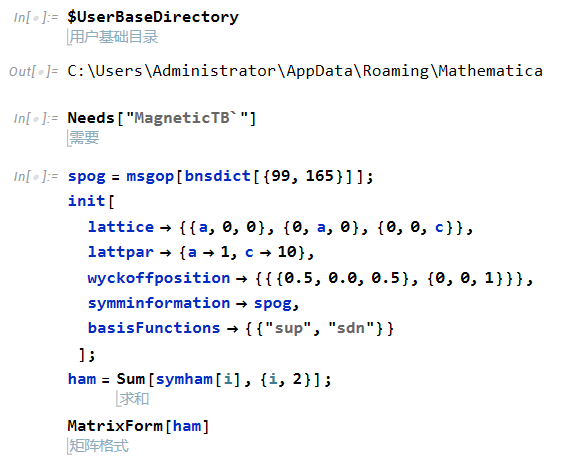
\includegraphics[max width=0.88\linewidth,max height=0.62\textheight,keepaspectratio]{assets/figure-8eaf301b7f1f.png}
\end{figure}\par\par


输出为:\par


\par\begin{figure}[H]\centering
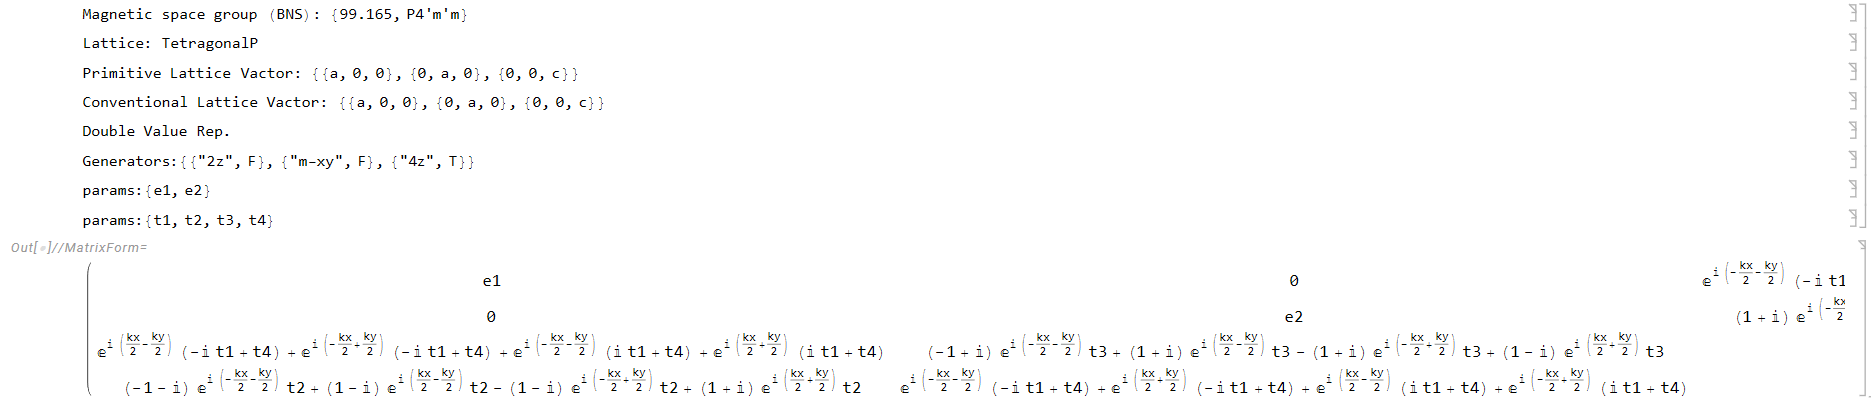
\includegraphics[max width=0.88\linewidth,max height=0.62\textheight,keepaspectratio]{assets/figure-77c40e47a7aa.png}
\end{figure}\par\par


然后运行下方代码,输出hr.dat紧束缚模型:\par


\par\begin{figure}[H]\centering
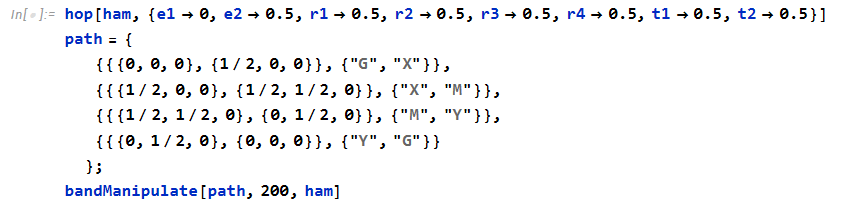
\includegraphics[max width=0.88\linewidth,max height=0.62\textheight,keepaspectratio]{assets/figure-64f2dcd3cbe8.png}
\end{figure}\par\par


上面是最基本的n能带模型构建代码,产生的hr.dat文件可以用于边缘态等紧束缚模型相关计算。\par


此外,为了探究e t r造成的影响,我写了进行拓扑相界扫描的代码,旨在一定的范围区间内,生成hr.dat文件,批量计算其拓扑不变量和能带,最后绘制出散点图,但由于维度过高,12能带模型的拓扑相界无法用 常规手段表征,且我是自行研究,无人指导,因此先记录,后如果涉及到相关领域,再继续研究,\par


\par\begin{figure}[H]\centering
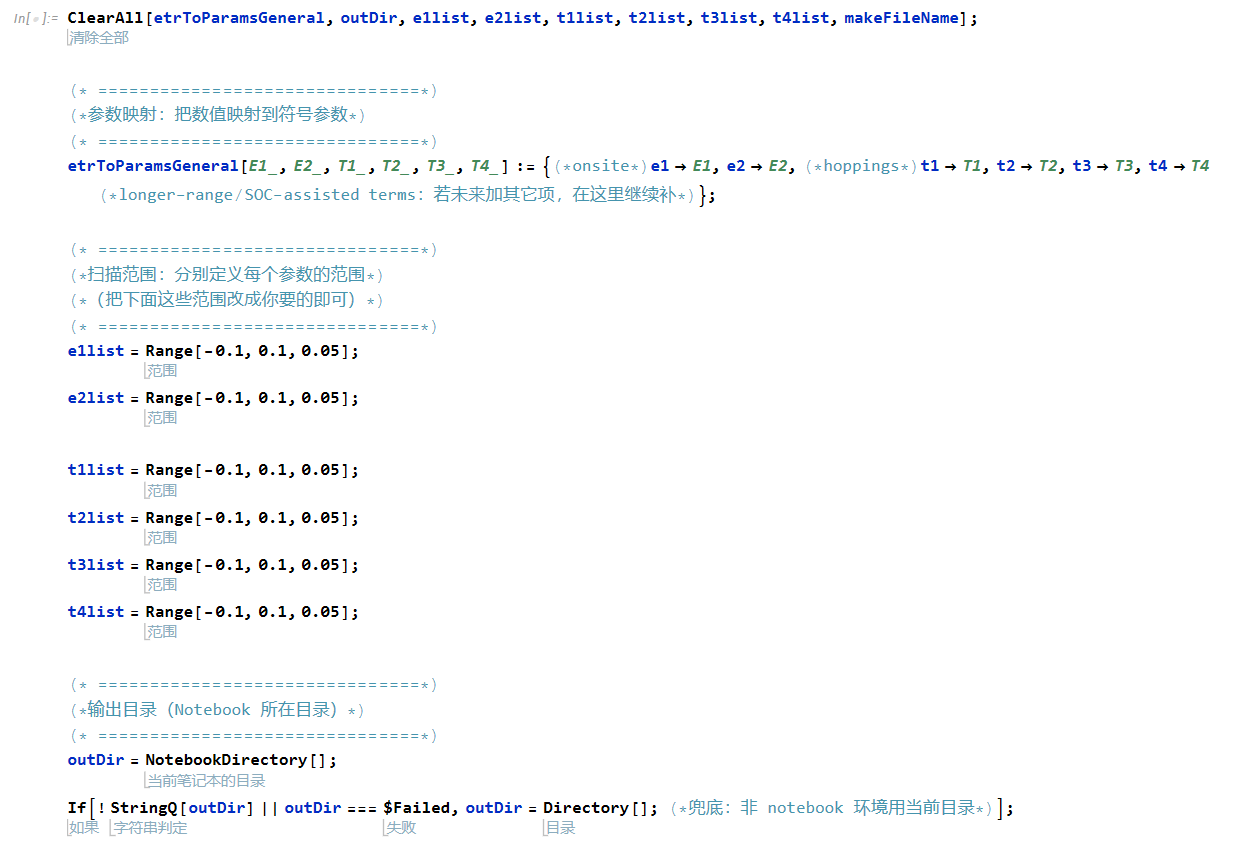
\includegraphics[max width=0.88\linewidth,max height=0.62\textheight,keepaspectratio]{assets/figure-8cf888eb4866.png}
\end{figure}\par
 
\par\begin{figure}[H]\centering
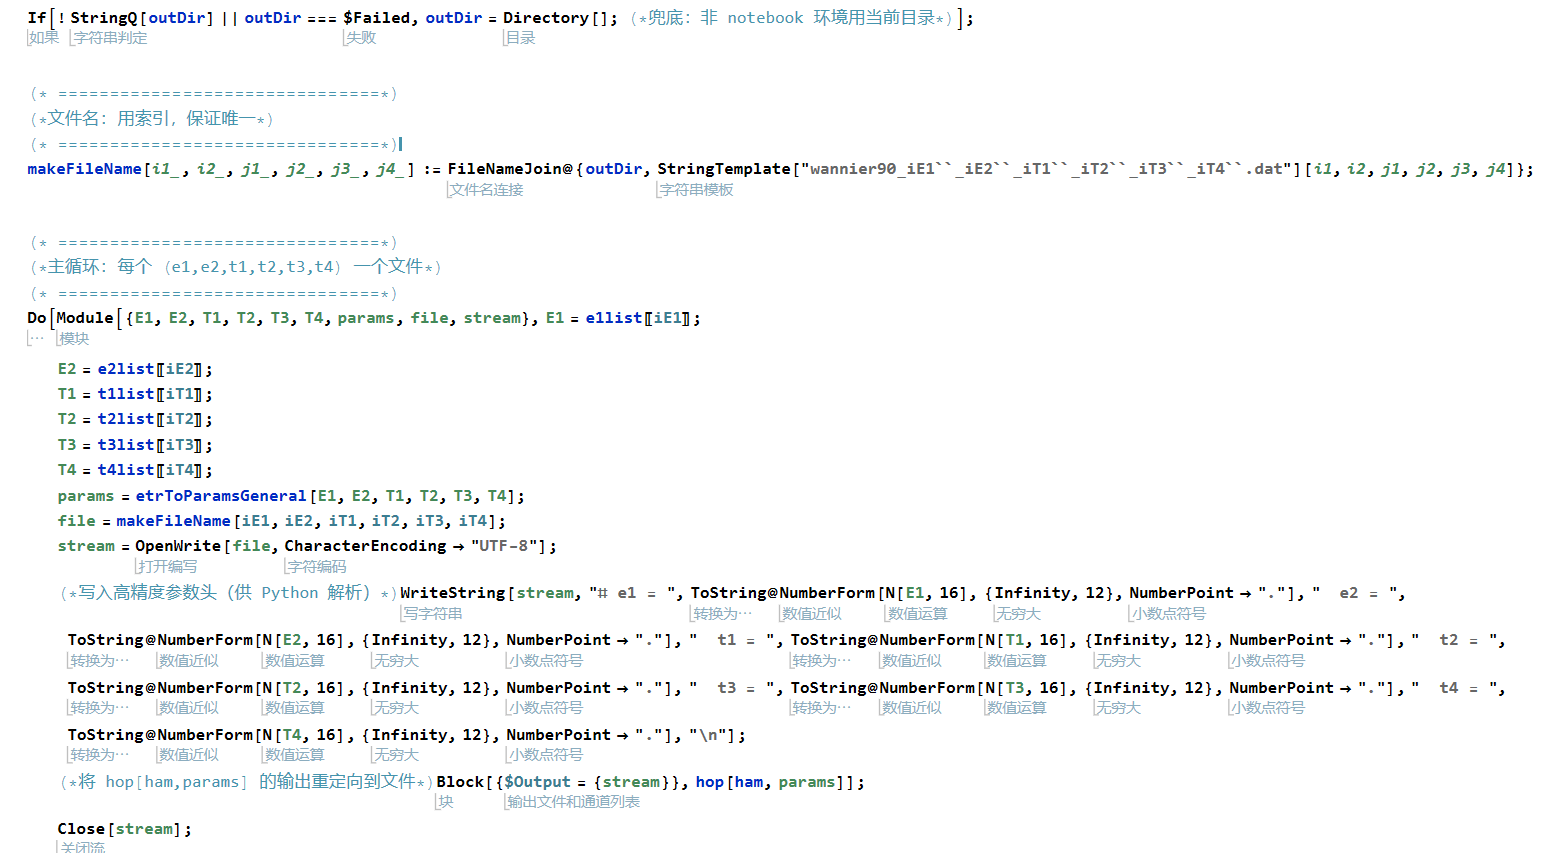
\includegraphics[max width=0.88\linewidth,max height=0.62\textheight,keepaspectratio]{assets/figure-d935cbb83dc1.png}
\end{figure}\par
 
\par\begin{figure}[H]\centering
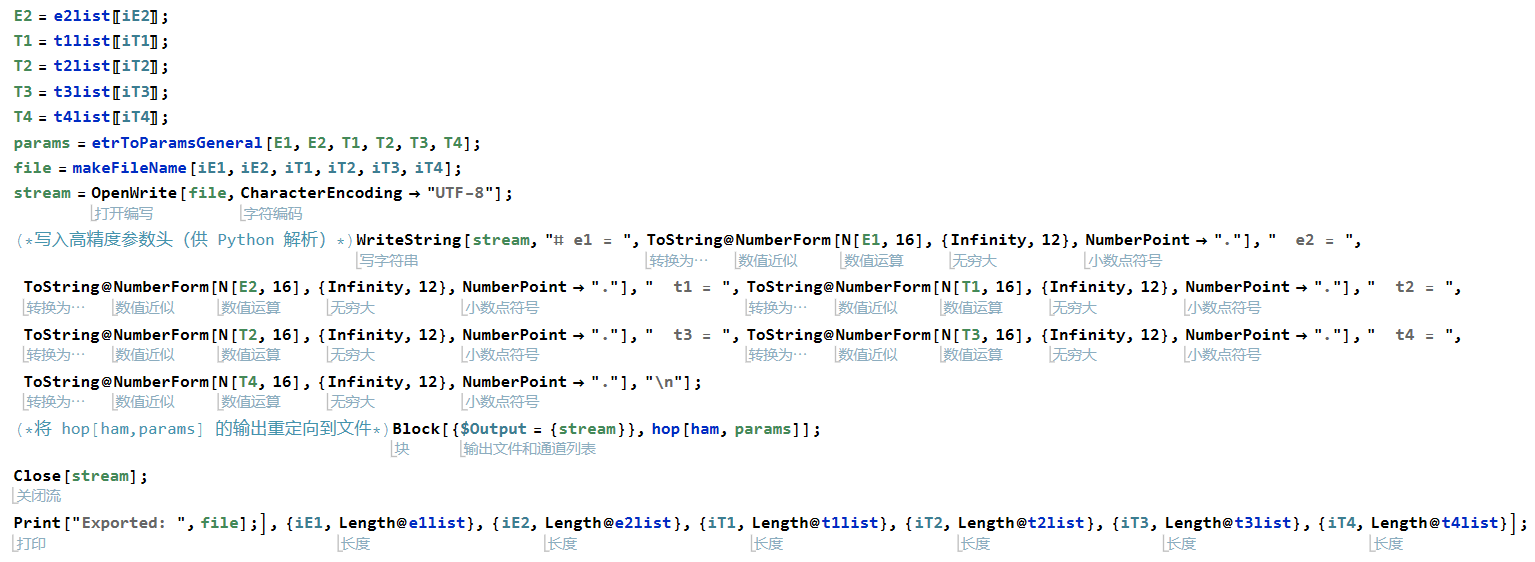
\includegraphics[max width=0.88\linewidth,max height=0.62\textheight,keepaspectratio]{assets/figure-fca0d9955ed0.png}
\end{figure}\par
 
\par\begin{figure}[H]\centering
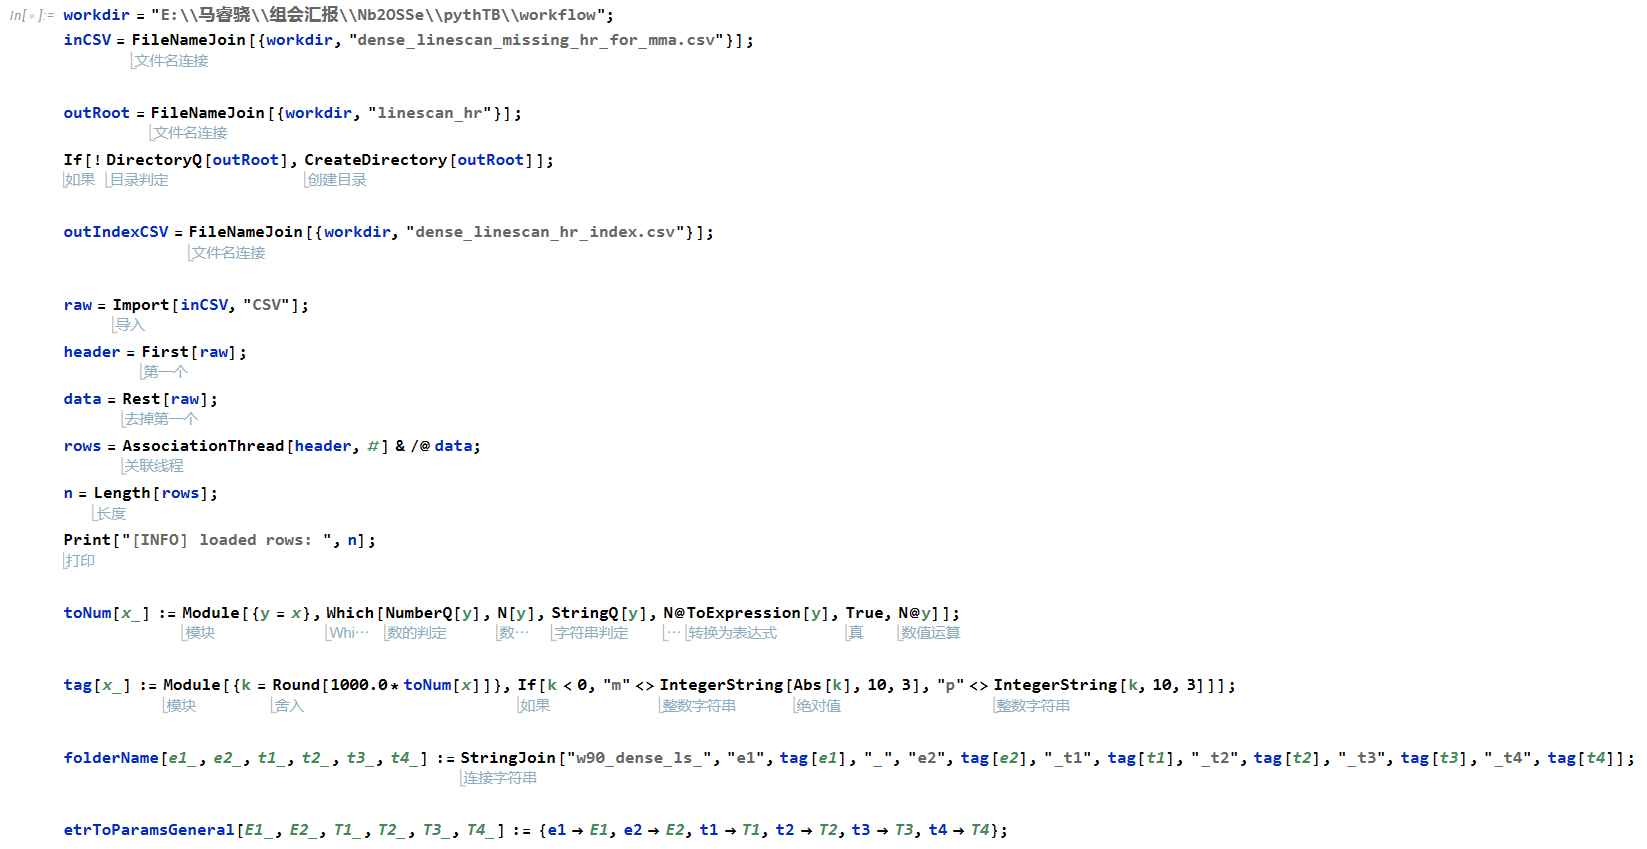
\includegraphics[max width=0.88\linewidth,max height=0.62\textheight,keepaspectratio]{assets/figure-d8257bd892e4.png}
\end{figure}\par
 
\par\begin{figure}[H]\centering
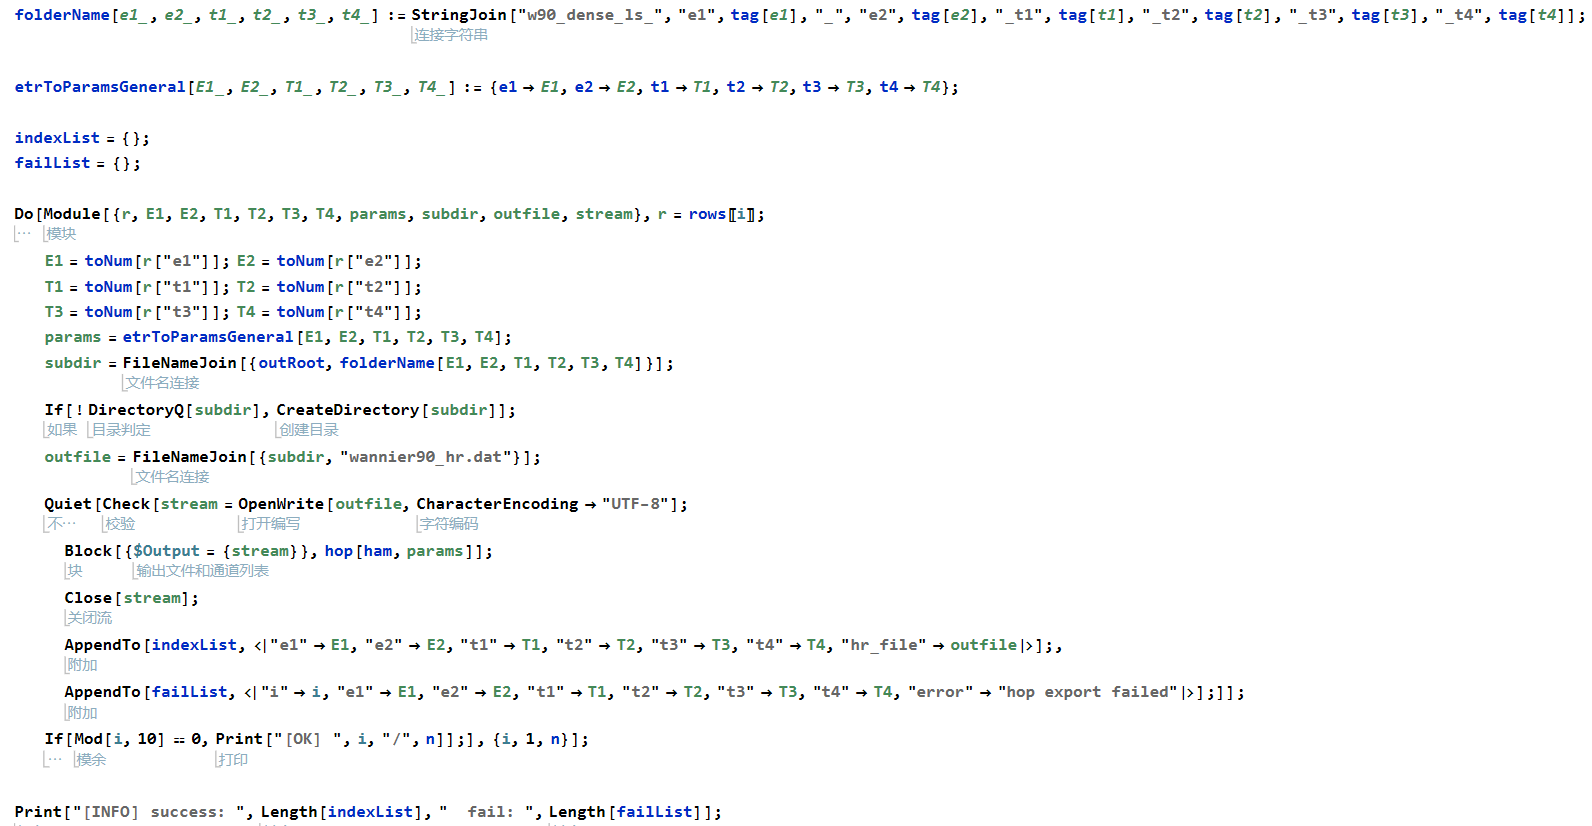
\includegraphics[max width=0.88\linewidth,max height=0.62\textheight,keepaspectratio]{assets/figure-f4da1ee86cd4.png}
\end{figure}\par
 
\par\begin{figure}[H]\centering
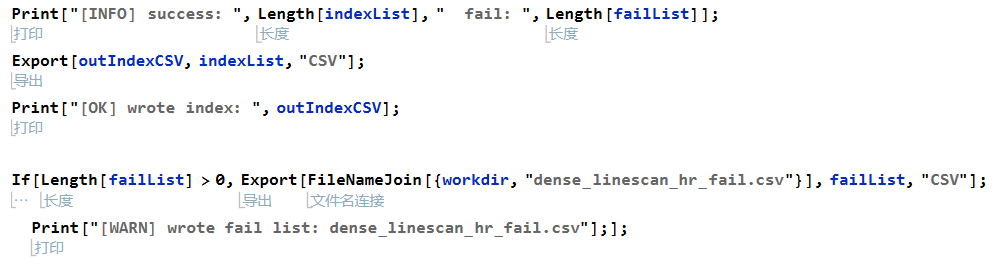
\includegraphics[max width=0.88\linewidth,max height=0.62\textheight,keepaspectratio]{assets/figure-3e73d965de87.png}
\end{figure}\par\par


完整代码只需要修改路径即可,我把输入文件上传到github,后面再补写文章。\par


后续用optuna进行超参数优化,这个是另一个方法(另一个python库)\par



\section{(原创自研)利用wannier验证超超交换路径}
\begin{articlemeta}
\textbf{日期：}2026-02-04\hfill\textbf{在线原文：}\href{https://marx2001.github.io/sci-note\_posts/20260204-super1}{marx2001.github.io}
\end{articlemeta}

\subsubsection{说明}


为验证MNX2Y6体系铁磁基态的产生机制,用wannier提取跃迁矩阵元,判断哪个元素主导超超交换路径。\par


1step.py 是提取在位能,2step.py是对各个原子进行超超交换路径组合,然后除以对应的在位能,形成一个值,根据这个值的大小判断超超交换路径贡献,找到路径最大的那个。\par


\subsubsection{代码的基本用法}


(1)第一步,将 Wannier 轨道“编号”与“物理含义”一一对应,也就是建立一张 WF index →(原子、轨道类型、位置) 的映射表。缺少这张表时,从 wannier90\_\allowbreak{}hr.dat 抽出来的矩阵元只是数字,无法明确其对应 Tc–Se、Se–Ir 还是 Tc–Tc 的哪条路径。\par


准备文件\par


\begin{codeindexbox}{代码清单 A.57.1}
语言：python；完整代码见附录第 \pageref{code:57:1} 页，共 3 行。
\end{codeindexbox}


即,第一步要确认wannier90拟合的正确性,并输出上述文件。\par


(2) Step 2 的核心是:将 wannier90\_\allowbreak{}hr.dat 里的 Hmn(R)变成“带几何距离的 hopping 列表”,再按目标子空间对(Tc–Tc、Tc–Se、Se–Ir...)和壳层做统计。\par


workflow:\par


准备:\par


\begin{codeindexbox}{代码清单 A.57.2}
语言：python；完整代码见附录第 \pageref{code:57:2} 页，共 3 行。
\end{codeindexbox}


输出:\par


\begin{codeindexbox}{代码清单 A.57.3}
语言：python；完整代码见附录第 \pageref{code:57:3} 页，共 2 行。
\end{codeindexbox}


名字随意,可以通过代码修改\par


代码:\par


\begin{codeindexbox}{代码清单 A.57.4}
语言：python；完整代码见附录第 \pageref{code:57:4} 页，共 357 行。
\end{codeindexbox}


命令行输入:\par


\begin{inlinecodebox}{命令示例 · shell}
\VerbatimInput[fontsize=\small,breaklines=true,breakanywhere=true,tabsize=2,listparameters={\setlength{\topsep}{0pt}\setlength{\partopsep}{0pt}\setlength{\parsep}{0pt}}]{code/057-005.sh}
\end{inlinecodebox}


可以调整命令来规定输出文件名\par


(3) 读取已经生成的 2step.csv(跨原子 edges),自动筛选 Tc–Se 与 Se–Ir 的近邻 hopping,构 造 Tc → Se → Ir → Se → Tc 的候选“超超交换路径”,并按路径权重排序输出一个csv文件。\par


对于三跳跃体系,类似超交换,可用下方脚本:\par


\begin{codeindexbox}{代码清单 A.57.6}
语言：python；完整代码见附录第 \pageref{code:57:6} 页，共 271 行。
\end{codeindexbox}


运行方法(针对当前文件名:2step.csv):\par


\begin{codeindexbox}{代码清单 A.57.7}
语言：shell；完整代码见附录第 \pageref{code:57:7} 页，共 7 行。
\end{codeindexbox}


如果尽可能不漏(慢):\par


\begin{codeindexbox}{代码清单 A.57.8}
语言：shell；完整代码见附录第 \pageref{code:57:8} 页，共 7 行。
\end{codeindexbox}


上面这个脚本没有测试过,使用需谨慎。\par


四跃迁桥连结构\par


\begin{codeindexbox}{代码清单 A.57.9}
语言：python；完整代码见附录第 \pageref{code:57:9} 页，共 265 行。
\end{codeindexbox}


使用方法:\par


\begin{inlinecodebox}{命令示例 · shell}
\VerbatimInput[fontsize=\small,breaklines=true,breakanywhere=true,tabsize=2,listparameters={\setlength{\topsep}{0pt}\setlength{\partopsep}{0pt}\setlength{\parsep}{0pt}}]{code/057-010.sh}
\end{inlinecodebox}


\begin{inlinecodebox}{命令示例 · shell}
\VerbatimInput[fontsize=\small,breaklines=true,breakanywhere=true,tabsize=2,listparameters={\setlength{\topsep}{0pt}\setlength{\partopsep}{0pt}\setlength{\parsep}{0pt}}]{code/057-011.sh}
\end{inlinecodebox}


分别输出Ge和Ir\par


源文件目录:/\allowbreak{}public/\allowbreak{}home/\allowbreak{}cssong/\allowbreak{}song/\allowbreak{}1mrx/\allowbreak{}9\_\allowbreak{}single\_\allowbreak{}layer/\allowbreak{}19\_\allowbreak{}ReIrGe2S6/\allowbreak{}TcIrGeSe/\allowbreak{} 3\_\allowbreak{}static\_\allowbreak{}band/\allowbreak{}4\_\allowbreak{}wannier/\allowbreak{}ncl\par


(4) 根据研究目标,需要判断超超交换路径主要由提供铁电性的迁移原子 Ge 还是非磁性原子 Ir 主导, 我们可以修改脚本,让它在输出路径时能够分别计算 Ge 和 Ir 路径的贡献,并将这些路径的 权重贡献 和参与原子频率明确标识出来。\par


这一步与(3)不矛盾,但代码有所不同,选择(4)也许更准一些。\par


\begin{codeindexbox}{代码清单 A.57.12}
语言：python；完整代码见附录第 \pageref{code:57:12} 页，共 224 行。
\end{codeindexbox}


要依次修改delta\_\allowbreak{}floor的值来确保全局不会因为分子过小而导致错误。分别测试0.1,0.5,1 。\par


(5) 与DFT结果的对比\par


上述代码都是从全局角度分析Ir和Ge究竟谁占超超交换的主导,而J1是DFT计算得到的J的主导,通过在 TB模型中计算J1元素分辨,来判断谁的贡献更大,代码如下:\par


\begin{codeindexbox}{代码清单 A.57.13}
语言：python；完整代码见附录第 \pageref{code:57:13} 页，共 46 行。
\end{codeindexbox}


运行方法:\par


\begin{inlinecodebox}{命令示例 · shell}
\VerbatimInput[fontsize=\small,breaklines=true,breakanywhere=true,tabsize=2,listparameters={\setlength{\topsep}{0pt}\setlength{\partopsep}{0pt}\setlength{\parsep}{0pt}}]{code/057-014.sh}
\end{inlinecodebox}


上述依据:\par


\par\begin{figure}[H]\centering
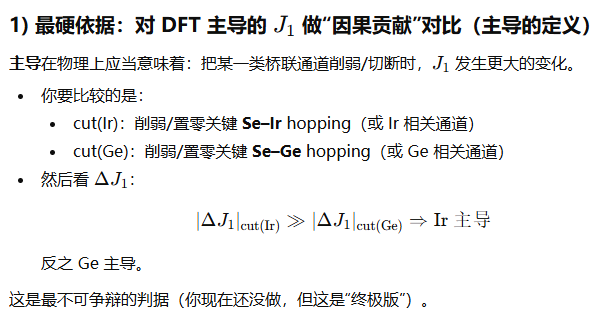
\includegraphics[max width=0.88\linewidth,max height=0.62\textheight,keepaspectratio]{assets/figure-131c738168c6.png}
\end{figure}\par
 
\par\begin{figure}[H]\centering
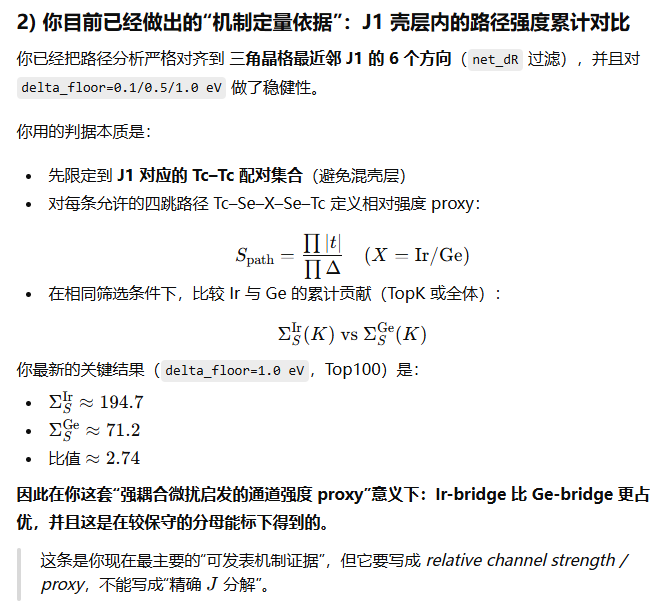
\includegraphics[max width=0.88\linewidth,max height=0.62\textheight,keepaspectratio]{assets/figure-23cf9091990d.png}
\end{figure}\par
 
\par\begin{figure}[H]\centering
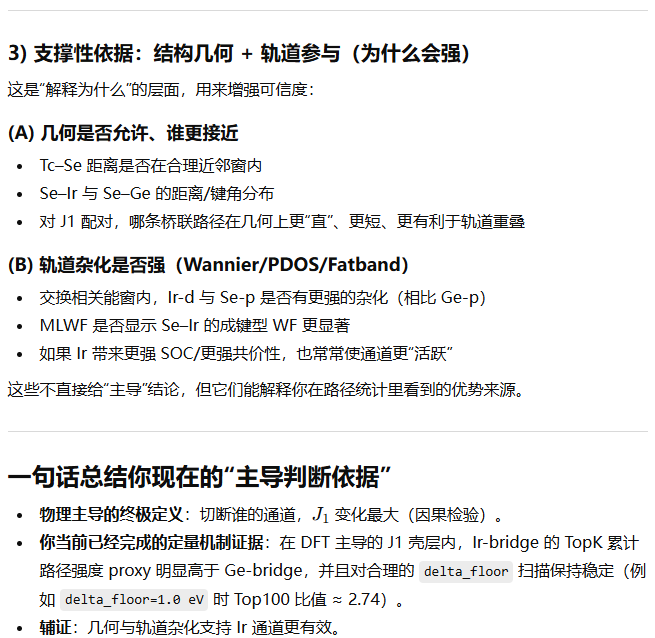
\includegraphics[max width=0.88\linewidth,max height=0.62\textheight,keepaspectratio]{assets/figure-ce796e5cbecb.png}
\end{figure}\par\par


\subsubsection{实际应用}


比较Ir和Ge哪个贡献更大(上面已经完成),下方是在不考虑soc的情况下,分别对spin up和spin down进行贡献比较,确保spin up能代表性的指出交换路径是d-p杂化组成的。\par


(1) 产生1step文件\par


\begin{codeindexbox}{代码清单 A.57.15}
语言：shell；完整代码见附录第 \pageref{code:57:15} 页，共 3 行。
\end{codeindexbox}


(2) 产生2step文件\par


\begin{codeindexbox}{代码清单 A.57.16}
语言：shell；完整代码见附录第 \pageref{code:57:16} 页，共 7 行。
\end{codeindexbox}


(3)与DFT进行对比\par


\begin{inlinecodebox}{命令示例 · shell}
\VerbatimInput[fontsize=\small,breaklines=true,breakanywhere=true,tabsize=2,listparameters={\setlength{\topsep}{0pt}\setlength{\partopsep}{0pt}\setlength{\parsep}{0pt}}]{code/057-017.sh}
\end{inlinecodebox}


这一步的输出类似于\par


\begin{codeindexbox}{代码清单 A.57.18}
语言：shell；完整代码见附录第 \pageref{code:57:18} 页，共 5 行。
\end{codeindexbox}


结论是,Ir比Ge贡献大的多,经过改变dleta\_\allowbreak{}floor,也是一样的结论,spin up和spin down并不能在数量上严格一致,但只要都支持d-p-d-p-d结论即可,用前面的评分标准定量分析,用MLWFS 的spin up通道定性演示(因为spin down的图极为混乱,看不清化学键)\par



\section{(原创自研)利用wannier验证超超交换路径(2)}
\begin{articlemeta}
\textbf{日期：}2026-02-06\hfill\textbf{在线原文：}\href{https://marx2001.github.io/sci-note\_posts/20260206-super2}{marx2001.github.io}
\end{articlemeta}

\subsubsection{说明}


上一篇文章是固定d-p-d-p-d的超超交换路径,dp杂化,而不能排除d-p-p-p-d杂化的可能,因此本篇文章通过修改脚本主要探究d-p-p-p-d杂化与d-p-d-p-d哪个更占据主导。 1step.py 是提取在位能,2step.py是对各个原子进行超超交换路径组合,然后除以对应的在位能,形成一个值,根据这个值的大小判断超超交换路径贡献,找到路径最大的那个。\par


\subsubsection{代码}


(1) 此次要在同一个子空间内对比Ge-d和Ge-p的超超交换路径评分,且考虑SOC,因此考虑下方的轨道:\par


\begin{codeindexbox}{代码清单 A.58.1}
语言：python；完整代码见附录第 \pageref{code:58:1} 页，共 6 行。
\end{codeindexbox}


运行一次成功的wannier拟合之后,进入第二步\par


(2) 我们需要重新修改一下代码,因为之前的代码是硬编码wannier centres和元素轨道对应。\par


\begin{codeindexbox}{代码清单 A.58.2}
语言：python；完整代码见附录第 \pageref{code:58:2} 页，共 536 行。
\end{codeindexbox}


运行指令\par


\begin{inlinecodebox}{短代码 · python}
\VerbatimInput[fontsize=\small,breaklines=true,breakanywhere=true,tabsize=2,listparameters={\setlength{\topsep}{0pt}\setlength{\partopsep}{0pt}\setlength{\parsep}{0pt}}]{code/058-003.py}
\end{inlinecodebox}


得到文件\par


\begin{codeindexbox}{代码清单 A.58.4}
语言：shell；完整代码见附录第 \pageref{code:58:4} 页，共 2 行。
\end{codeindexbox}


\begin{codeindexbox}{代码清单 A.58.5}
语言：python；完整代码见附录第 \pageref{code:58:5} 页，共 430 行。
\end{codeindexbox}


运行指令\par


\begin{inlinecodebox}{短代码 · python}
\VerbatimInput[fontsize=\small,breaklines=true,breakanywhere=true,tabsize=2,listparameters={\setlength{\topsep}{0pt}\setlength{\partopsep}{0pt}\setlength{\parsep}{0pt}}]{code/058-006.py}
\end{inlinecodebox}


重复运行上面指令,得到Ge-d和Ge-p的评分\par


然后增大delta\_\allowbreak{}floor确保数值稳定,如果出现不一致,那么说明脚本或者公式存在问题,需要重新考虑。\par


目前我的材料体系得到的结果是Ge-d相比于Ir-d和Ge-p,Ge-d参与的评分更高,但是dos和投影能带指出,费米能级附近的主要贡献是Ge-p,所以考虑Ge-d轨道是不合适的。\par


所以真正的结论是,这是一个d-p-d-p-d的超超交换路径。\par


最终结论,经过详实的对超超交换路径的评分,落实了d-p杂化导致的强铁磁基态,且是四面体配位的Se原子路径。\par



\section{(原创自研)利用wannier验证超超交换路径(3)}
\begin{articlemeta}
\textbf{日期：}2026-02-07\hfill\textbf{在线原文：}\href{https://marx2001.github.io/sci-note\_posts/20260207-super3}{marx2001.github.io}
\end{articlemeta}

\subsubsection{说明}


上一篇文章是固定d-p-d-p-d的超超交换路径,dp杂化,而不能排除d-p-p-p-d杂化的可能,因此本篇文章通过修改脚本主要探究d-p-p-p-d杂化与d-p-d-p-d哪个更占据主导。 1step.py 是提取在位能,2step.py是对各个原子进行超超交换路径组合,然后除以对应的在位能,形成一个值,根据这个值的大小判断超超交换路径贡献,找到路径最大的那个。\par


这篇文章是细化成能用于论文的指标,包括在位能等等。\par


文件路径:\par


\begin{inlinecodebox}{命令示例 · shell}
\VerbatimInput[fontsize=\small,breaklines=true,breakanywhere=true,tabsize=2,listparameters={\setlength{\topsep}{0pt}\setlength{\partopsep}{0pt}\setlength{\parsep}{0pt}}]{code/059-001.sh}
\end{inlinecodebox}


\subsubsection{代码}


(1) 第一步\par


之前的脚本里虽然已经做了 WF centre → 最近原子(PBC minimum image)的映射(map\_\allowbreak{}wf\_\allowbreak{}to\_\allowbreak{}atoms),但真正用于分组(Tc\_\allowbreak{}d/\allowbreak{}Ir\_\allowbreak{}d/\allowbreak{}Se\_\allowbreak{}p/\allowbreak{}Ge\_\allowbreak{}p)的仍然是硬编码的 WF 序号区间 wf\_\allowbreak{}group。并且在主循环里 gm = wf\_\allowbreak{}group(m), gn = wf\_\allowbreak{}group(n) 也仍然走的是这个硬编码逻辑。这就导致:只要投影顺序、num\_\allowbreak{}wann、spin 通道或 Wannier 排序发生变化,分组 就会错——因此”之前修改是否正确”的结论是:核心问题没有被真正修掉(最近原子映射算出来了,但没用来分组)。\par


下文对该脚本进行了”最小但关键”的正确修复:删除 wf\_\allowbreak{}group(wf) 的”WF 序号区间分组”(这是不可靠的根源),改为:对每条 hopping,先使用已计算出的 elem\_\allowbreak{}m/\allowbreak{}elem\_\allowbreak{}n(来自最 近原子映射),再进行无向格式(便于做壳层统计),同时在 out\_\allowbreak{}edges 里额外写出 group\_\allowbreak{}m/\allowbreak{}group\_\allowbreak{}n,便于后续在 2step 中筛选。\par


\begin{codeindexbox}{代码清单 A.59.2}
语言：python；完整代码见附录第 \pageref{code:59:2} 页，共 402 行。
\end{codeindexbox}


运行方法:\par


\begin{inlinecodebox}{短代码 · python}
\VerbatimInput[fontsize=\small,breaklines=true,breakanywhere=true,tabsize=2,listparameters={\setlength{\topsep}{0pt}\setlength{\partopsep}{0pt}\setlength{\parsep}{0pt}}]{code/059-003.py}
\end{inlinecodebox}


(2) 第二步是优化2step.py,对应1step.py\par


当前脚本虽然已经建立了Wannier函数中心到最近原子的映射,但其用于轨道分组的核心逻辑仍然依赖于硬编码的Wannier函数序号区间。具体来说,在主循环中判断Tc\_\allowbreak{}d、Ir\_\allowbreak{}d等分组依据的 wf\_\allowbreak{}group()函数,正是基于此不可靠的序号范围。这导致一旦体系的投影顺序、Wannier函数数量、自旋通道设置发生改变,或Wannier函数本身经过重排,分组结果必然出错。因此,之前对脚本的 修改并未触及这一根本问题,已计算出的原子映射信息实际上并未被用于关键的分组步骤。\par


为解决此问题,需要进行一项关键修复:彻底删除基于序号区间的wf\_\allowbreak{}group函数。正确的做法是,在处理每条hopping时,直接利用已计算出的elem\_\allowbreak{}m/\allowbreak{}elem\_\allowbreak{}n(即映射得到的原子元素信 息),再通过一个可配置的、从元素到轨道组的映射关系(例如Tc-> Tc\_\allowbreak{}d),来动态确定分组标签。同时,建议通过新增命令行参数来接收此映射关系及分组顺序,这将使脚本完全脱离对特定体系 编码的依赖,增强通用性。输出方面,pair列可继续保持Tc\_\allowbreak{}d<->Se\_\allowbreak{}p这类无向格式以利于统计,但需在结果中额外输出group\_\allowbreak{}m/\allowbreak{}group\_\allowbreak{}n两列,以便后续的2step.py脚本能够依据准确的分组信息 进行筛选和计算。\par


目前的 1step 输出已包含 group\_\allowbreak{}m/\allowbreak{}group\_\allowbreak{}n列(例如 Tc\_\allowbreak{}d、Se\_\allowbreak{}p 等),因此 2step 的核心改进在于:应优先依据这些明确的分组信息来筛选路径和建边,而不再依赖原始的 elem\_\allowbreak{}m/\allowbreak{}elem\_\allowbreak{}n (如 “Tc”、”Se” 等元素标签)。这一调整将彻底避免对不稳定的“Wannier 函数序号范围”的依赖。\par


为了实现平滑过渡,对 2step 进行如下修改:新版将兼容两种输入格式。当输入文件包含 group\_\allowbreak{}m/\allowbreak{}group\_\allowbreak{}n列时,程序会优先使用分组信息;若为旧格式文件,则自动回退至基于 elem\_\allowbreak{}m/\allowbreak{}elem\_\allowbreak{}n 的逻辑。本次改动将在其基础上以“最小侵入”的方式完成,确保核心流程清晰且易于维护。\par


\begin{codeindexbox}{代码清单 A.59.4}
语言：python；完整代码见附录第 \pageref{code:59:4} 页，共 386 行。
\end{codeindexbox}


使用方法:\par


\begin{inlinecodebox}{短代码 · python}
\VerbatimInput[fontsize=\small,breaklines=true,breakanywhere=true,tabsize=2,listparameters={\setlength{\topsep}{0pt}\setlength{\partopsep}{0pt}\setlength{\parsep}{0pt}}]{code/059-005.py}
\end{inlinecodebox}


(3) 第三步,新增考虑U和J。\par


下面提供一份完整且可直接替换的 2step.py脚本。该版本在我之前提交的“带 U/\allowbreak{}JH 分母修正”基础上,进一步针对当前体系的特点做了适配调整。\par


在参数设置上,默认 hund\_\allowbreak{}coef取值为 2(对应更合理的 U + 2JH形式,这是考虑到体系中 d 轨道呈 2+2+1 分裂的实际情况,因此不建议默认使用 4)。同时保留 –hund\_\allowbreak{}coef 参数,可设置为 1、2、4 等不同取值,以进行敏感性分析。\par


功能方面,保留了 –enable\_\allowbreak{}UJ开关:开启时将使用包含 U 和 JH 的分母进行计算;关闭则回退到仅依赖 on-site 能级差的纯能量分母模式。为了方便论文写作与结果复现,输出 CSV 文件中会 新增记录相关参数,包括:enable\_\allowbreak{}UJ、U\_\allowbreak{}Tc、U\_\allowbreak{}Ir、JH\_\allowbreak{}Tc、JH\_\allowbreak{}Ir以及 hund\_\allowbreak{}coef。\par


需要说明的是,此版本默认采用元素模式(即识别 Tc、Se、Ir 等元素标签)。如果 edges.csv中已包含 group\_\allowbreak{}m/\allowbreak{}group\_\allowbreak{}n列(例如 Tc\_\allowbreak{}d、Se\_\allowbreak{}p、Ir\_\allowbreak{}d),并希望依据这些分组信息进行处理, 请运行时添加以下参数\par


\begin{codeindexbox}{代码清单 A.59.6}
语言：python；完整代码见附录第 \pageref{code:59:6} 页，共 472 行。
\end{codeindexbox}


使用方法:\par


\begin{inlinecodebox}{短代码 · python}
\VerbatimInput[fontsize=\small,breaklines=true,breakanywhere=true,tabsize=2,listparameters={\setlength{\topsep}{0pt}\setlength{\partopsep}{0pt}\setlength{\parsep}{0pt}}]{code/059-007.py}
\end{inlinecodebox}


(4)第四步,筛选各个原子链\par


选择各个原子链中,评分排名前3的原子链\par


\begin{codeindexbox}{代码清单 A.59.8}
语言：python；完整代码见附录第 \pageref{code:59:8} 页，共 140 行。
\end{codeindexbox}


使用方法:\par


\begin{inlinecodebox}{短代码 · python}
\VerbatimInput[fontsize=\small,breaklines=true,breakanywhere=true,tabsize=2,listparameters={\setlength{\topsep}{0pt}\setlength{\partopsep}{0pt}\setlength{\parsep}{0pt}}]{code/059-009.py}
\end{inlinecodebox}


使用两次,考虑netR\par


\begin{inlinecodebox}{短代码 · python}
\VerbatimInput[fontsize=\small,breaklines=true,breakanywhere=true,tabsize=2,listparameters={\setlength{\topsep}{0pt}\setlength{\partopsep}{0pt}\setlength{\parsep}{0pt}}]{code/059-010.py}
\end{inlinecodebox}


(5) 第五步 提取超超交换各个原子之间的跃迁参数\par


运行下方代码:\par


\begin{codeindexbox}{代码清单 A.59.11}
语言：python；完整代码见附录第 \pageref{code:59:11} 页，共 86 行。
\end{codeindexbox}


使用方法:\par


\begin{inlinecodebox}{短代码 · python}
\VerbatimInput[fontsize=\small,breaklines=true,breakanywhere=true,tabsize=2,listparameters={\setlength{\topsep}{0pt}\setlength{\partopsep}{0pt}\setlength{\parsep}{0pt}}]{code/059-012.py}
\end{inlinecodebox}


(6) 第六步 提取Tc之间直接交换,与超超交换强度的数量级作比较\par


\begin{codeindexbox}{代码清单 A.59.13}
语言：python；完整代码见附录第 \pageref{code:59:13} 页，共 121 行。
\end{codeindexbox}


使用方法:\par


\begin{inlinecodebox}{短代码 · python}
\VerbatimInput[fontsize=\small,breaklines=true,breakanywhere=true,tabsize=2,listparameters={\setlength{\topsep}{0pt}\setlength{\partopsep}{0pt}\setlength{\parsep}{0pt}}]{code/059-014.py}
\end{inlinecodebox}


至此,得到了超超交换路径与直接交换路径的定量表述。\par



\section{(原创自研)利用PDOS验证超超交换路径}
\begin{articlemeta}
\textbf{日期：}2026-02-08\hfill\textbf{在线原文：}\href{https://marx2001.github.io/sci-note\_posts/20260208-pdos}{marx2001.github.io}
\end{articlemeta}

\subsubsection{说明}


暂无\par


\subsubsection{代码}


用这个代码,计算出设置范围内的指定原子的价带顶和导带底的分轨道能级排布顺序。\par


\begin{codeindexbox}{代码清单 A.60.1}
语言：python；完整代码见附录第 \pageref{code:60:1} 页，共 297 行。
\end{codeindexbox}


使用方法\par


\begin{inlinecodebox}{命令示例 · shell}
\VerbatimInput[fontsize=\small,breaklines=true,breakanywhere=true,tabsize=2,listparameters={\setlength{\topsep}{0pt}\setlength{\partopsep}{0pt}\setlength{\parsep}{0pt}}]{code/060-002.sh}
\end{inlinecodebox}



\section{(原创自研)利用wannier验证超超交换路径(4)}
\begin{articlemeta}
\textbf{日期：}2026-02-08\hfill\textbf{在线原文：}\href{https://marx2001.github.io/sci-note\_posts/20260208-super4}{marx2001.github.io}
\end{articlemeta}

\subsubsection{说明}


本篇文章是此系列最后一篇文章,提取跃迁矩阵元,将其对角化后量化d轨道和p轨道的分轨道的相对能量并画图。 文件路径:\par


\begin{inlinecodebox}{命令示例 · shell}
\VerbatimInput[fontsize=\small,breaklines=true,breakanywhere=true,tabsize=2,listparameters={\setlength{\topsep}{0pt}\setlength{\partopsep}{0pt}\setlength{\parsep}{0pt}}]{code/061-001.sh}
\end{inlinecodebox}


\subsubsection{代码}


(1) 第一步\par


核心用途:从 Wannier90 的 wannier90\_\allowbreak{}hr.dat 里提取每个原子对应的“局域在位(on-site)哈密顿量”子块,做本征分解得到“局域能级”(可理解为晶场/\allowbreak{}原子轨道能级的数值化近似), 并且用 wannier90.win 的投影顺序给这些能级打上 px/\allowbreak{}py/\allowbreak{}pz/\allowbreak{}dxy/\allowbreak{}... 之类的轨道标签,最后输出若干 CSV 统计文件。\par


该脚本通过读取三个关键文件构建材料模型:\par


wannier90\_\allowbreak{}hr.dat(对应 –hr参数):提取 R=(0,0,0) 的矩阵元,构建 on‐site 哈密顿量并做厄米化处理(0.5*(H0+H0†))。\par


edges.csv(对应 –edges参数):提供 Wannier 函数与原子/\allowbreak{}元素的归属关系,必须包含 m,n,atom m,atom n,elem m,elem n列;若同一 WF 被标记为不同原子或元素,脚本会报错并要 求修正一致性。\par


wannier90.win(对应 –win参数):仅解析 begin projections...end projections块,获取各元素的投影轨道信息(支持自动将 d/\allowbreak{}p/\allowbreak{}s 展开为 5d/\allowbreak{}3p/\allowbreak{}1s)。\par


以上文件共同用于构建哈密顿量并关联轨道、原子与元素信息。\par


总的来说:专门用于分析Wannier函数局域能级的工具。它通过整合三份输入文件——hr.dat(提供哈密顿量矩阵元)、edges.csv(定义Wannier函数与原子的归属关系)和wannier90.win(规 定轨道的投影顺序)——来构建并分解每个原子附近的电子结构。\par


其核心计算流程分为六步:首先从哈密顿量中提取on-site相互作用部分;接着将Wannier函数按原子分组;然后依据投影信息为这些函数打上轨道标签;之后对每个原子的哈密顿量子块进行本 征分解,获得局域能级;再为每个能级标记出其主导轨道成分;最后还可选择性地进行能级配对诊断,以分析能级分裂特征。\par


脚本会输出三份CSV结果文件:levels.csv详细列出每个原子的所有能级及其主导轨道;pair\_\allowbreak{}centers.csv提供能级配对的诊断信息;orbital\_\allowbreak{}order.csv则汇总了每个原子各类轨道的最低 能量。总而言之,该工具将抽象的哈密顿量矩阵转化为清晰、按原子和轨道分解的能级图谱,极大地便利了后续的材料电子结构分析与可视化。\par


\begin{codeindexbox}{代码清单 A.61.2}
语言：python；完整代码见附录第 \pageref{code:61:2} 页，共 350 行。
\end{codeindexbox}


使用方法:\par


\begin{inlinecodebox}{命令示例 · shell}
\VerbatimInput[fontsize=\small,breaklines=true,breakanywhere=true,tabsize=2,listparameters={\setlength{\topsep}{0pt}\setlength{\partopsep}{0pt}\setlength{\parsep}{0pt}}]{code/061-003.sh}
\end{inlinecodebox}


(2) 第二步\par


这是一个用于分析材料中元素局域能级分布的Python脚本。其核心功能是对前序脚本(如 cf\_\allowbreak{}final hr\_\allowbreak{}win\_\allowbreak{}edges.py)生成的 *\_\allowbreak{}levels.csv文件进行高阶统计分析。\par


脚本首先对原始数据进行清洗,过滤掉主导轨道标签不可靠的能级(如轨道权重过低或为空),确保分析质量。随后,按“元素-主导轨道”组合进行分组,计算每个组内能级能量的详细统计量, 包括均值、标准差、分位数等。最重要的,脚本会汇总每个元素在不同轨道上的中位数能级,并通过计算其极差,生成一个衡量“晶场分裂强度”或“轨道能级展开”的实用摘要。\par


最终,脚本会输出三个CSV文件:一份包含所有有效能级的详细长表、一份每个元素-轨道组合的统计量表,以及一份汇总了各元素轨道能级展开范围的核心摘要,从而将原子尺度的复杂数据提炼 为元素层面的清晰物理图像。\par


\begin{codeindexbox}{代码清单 A.61.4}
语言：python；完整代码见附录第 \pageref{code:61:4} 页，共 95 行。
\end{codeindexbox}


使用方法:\par


\begin{inlinecodebox}{短代码 · python}
\VerbatimInput[fontsize=\small,breaklines=true,breakanywhere=true,tabsize=2,listparameters={\setlength{\topsep}{0pt}\setlength{\partopsep}{0pt}\setlength{\parsep}{0pt}}]{code/061-005.py}
\end{inlinecodebox}


(3) 第三步\par


该脚本(cfFINAL\_\allowbreak{}export\_\allowbreak{}fullweights.py)在材料电子结构分析中实现了关键增强。它首先读取三个必要文件:wannier90\_\allowbreak{}hr.dat(构建on-site哈密顿量)、edges.csv(建立Wannier 函数到原子的唯一映射)和wannier90.win(确定投影轨道顺序),并严格校验WF顺序与投影顺序的一致性以保证后续标签准确。\par


其核心计算分为两步:对每个原子的on-site哈密顿量子块进行对角化,得到局域能级;然后,对每条能级的本征态,计算其在所有基轨道(如px、py、pz、dxy等)上的详细权重分布。这是相 较于旧版工具的最大提升——旧版仅输出主导轨道,而新版会导出所有轨道的精确占比。\par


脚本最终输出三个CSV文件,其中最重要的*\_\allowbreak{}levels\_\allowbreak{}fullweights.csv文件完整记录了每条能级的全轨道权重。这使得用户可以直接提取特定元素(如硒Se)的所有px、py、pz轨道权重,进 而进行加权的分布统计、绘制能级展开图等深入分析,而不再局限于之前仅基于主导轨道的简化统计。\par


\begin{codeindexbox}{代码清单 A.61.6}
语言：python；完整代码见附录第 \pageref{code:61:6} 页，共 269 行。
\end{codeindexbox}


\begin{inlinecodebox}{命令示例 · shell}
\VerbatimInput[fontsize=\small,breaklines=true,breakanywhere=true,tabsize=2,listparameters={\setlength{\topsep}{0pt}\setlength{\partopsep}{0pt}\setlength{\parsep}{0pt}}]{code/061-007.sh}
\end{inlinecodebox}


(4) 第四步\par


collect\_\allowbreak{}elem\_\allowbreak{}orbital\_\allowbreak{}distributions.py脚本是用于分析材料中元素轨道能量分布的专业工具。其核心功能是基于包含全轨道权重的能级数据(*\_\allowbreak{}levels\_\allowbreak{}fullweights.csv),对每个元 素的各个轨道(如 Se 的 px、py、pz)进行加权统计,从而解决了此前提出的“分析Se的px/\allowbreak{}py/\allowbreak{}pz整体分布”的需求。\par


具体而言,它对每个元素和轨道(如 w\_\allowbreak{}px)执行以下计算:首先,将每条能级的相对能量 E\_\allowbreak{}rel视为样本值,并将其在该轨道上的权重 w\_\allowbreak{}orb作为样本权重;接着,过滤掉权重过小的噪声数 据;然后,计算加权平均值、标准差、分位数等统计量;最后,生成加权的能量分布直方图数据。\par


脚本默认输出两个CSV文件:一个汇总每个元素-轨道组合的加权统计数据(\emph{\_\allowbreak{}weighted\_\allowbreak{}stats.csv),另一个则提供用于绘制分布曲线或热图的直方图数据点(}\_\allowbreak{}hist.csv)。\par


与此前按主导轨道进行“硬分类”的脚本 collect\_\allowbreak{}elem\_\allowbreak{}cf\_\allowbreak{}stats.py不同,本脚本利用全轨道权重进行“软分解”统计,能更精确地刻画每个轨道对整体能级的贡献分布。\par


\begin{codeindexbox}{代码清单 A.61.8}
语言：python；完整代码见附录第 \pageref{code:61:8} 页，共 119 行。
\end{codeindexbox}


使用方法:\par


\begin{inlinecodebox}{命令示例 · shell}
\VerbatimInput[fontsize=\small,breaklines=true,breakanywhere=true,tabsize=2,listparameters={\setlength{\topsep}{0pt}\setlength{\partopsep}{0pt}\setlength{\parsep}{0pt}}]{code/061-009.sh}
\end{inlinecodebox}


(5) 第五步 绘图\par


配套的绘图工具,用于将前序统计分析的结果进行可视化。\par


plot\_\allowbreak{}elem\_\allowbreak{}level\_\allowbreak{}diagram.py 用于绘制元素的轨道能级示意图。它读取包含加权统计量(如中位数、四分位数)的文件,为指定元素的每个轨道绘制一条以加权中位能量为中心的水平线 段,并可选择添加四分位距区间以示意能级分布宽度。其产出类似一张简明的“能级图”,直观展示各轨道能量的中心位置与离散程度。\par


plot\_\allowbreak{}elem\_\allowbreak{}orb\_\allowbreak{}distributions.py 则用于绘制元素-轨道的能量分布曲线图。它基于直方图数据文件,为指定元素的每个轨道绘制一条完整的分布曲线,横轴为能量,纵轴为加权强度,从而 完整呈现每个轨道在能量空间中的分布形状、峰位和展宽。\par


两者的核心区别在于信息压缩程度:前者将每个轨道的信息压缩为一个代表性能级(可带误差棒),产出示意图;后者则保留并展示完整的分布轮廓,产出细节曲线图。它们从不同维度呈现同一 组数据,共同服务于对材料中元素局域电子结构的深入理解与展示。\par


\begin{codeindexbox}{代码清单 A.61.10}
语言：python；完整代码见附录第 \pageref{code:61:10} 页，共 88 行。
\end{codeindexbox}


\begin{codeindexbox}{代码清单 A.61.11}
语言：python；完整代码见附录第 \pageref{code:61:11} 页，共 84 行。
\end{codeindexbox}


使用方法\par


\begin{codeindexbox}{代码清单 A.61.12}
语言：shell；完整代码见附录第 \pageref{code:61:12} 页，共 10 行。
\end{codeindexbox}


(6)第六步 旋转坐标系\par


第五步的脚本相对于eg和t2g这种经典情况理论上是适用的,因为没有旋转局域坐标系,我的材料并不是通常的畸变情况,所以不适用,因此下方脚本是针对这个问题而写的。\par


\begin{codeindexbox}{代码清单 A.61.13}
语言：python；完整代码见附录第 \pageref{code:61:13} 页，共 583 行。
\end{codeindexbox}


使用方法:\par


\begin{inlinecodebox}{命令示例 · shell}
\VerbatimInput[fontsize=\small,breaklines=true,breakanywhere=true,tabsize=2,listparameters={\setlength{\topsep}{0pt}\setlength{\partopsep}{0pt}\setlength{\parsep}{0pt}}]{code/061-014.sh}
\end{inlinecodebox}


这个脚本确实有效,但是由于wannier考虑soc是一种较为”混乱“的情况,包含了杂化等等,所以即使旋转了坐标系,也是不能实现和dft计算中的pdos同样的简并情况。\par


(7)第七步 通过pdos中的d轨道\par


计算bandcenters,得到准确的轨道能级分布。\par


输入文件,dft计算dos后,用vaspkit导出的数据文档。\par


\begin{codeindexbox}{代码清单 A.61.15}
语言：python；完整代码见附录第 \pageref{code:61:15} 页，共 2 行。
\end{codeindexbox}


代码如下:\par


\begin{codeindexbox}{代码清单 A.61.16}
语言：python；完整代码见附录第 \pageref{code:61:16} 页，共 121 行。
\end{codeindexbox}


运行代码,能量范围-1到0,价带顶:\par


\begin{inlinecodebox}{命令示例 · shell}
\VerbatimInput[fontsize=\small,breaklines=true,breakanywhere=true,tabsize=2,listparameters={\setlength{\topsep}{0pt}\setlength{\partopsep}{0pt}\setlength{\parsep}{0pt}}]{code/061-017.sh}
\end{inlinecodebox}


该脚本的核心原理:将轨道投影态密度(PDOS)视为能量分布函数 Dα(E),在用户指定的能量窗口内,通过计算其一阶矩(即“带中心”)来定义每个轨道或轨道组的有效能量位置, 并利用其零阶矩(积分面积)来量化该轨道在该窗口内的总谱权重。\par


该原理的适用范围及学术写作中的准确表述方式。该方法提供的是基于PDOS的“有效能级对齐”,而非来自局域哈密顿量的严格晶场本征值。在用于绘制轨道能级示意图并解释超交换等 机制时,建议在论文中表述为“根据占据能窗内的轨道投影态密度谱重中心确定各轨道组的相对能量位置”,这样的表述更为严谨。\par


然后绘图\par


\begin{codeindexbox}{代码清单 A.61.18}
语言：python；完整代码见附录第 \pageref{code:61:18} 页，共 208 行。
\end{codeindexbox}


使用方法\par


\begin{inlinecodebox}{命令示例 · shell}
\VerbatimInput[fontsize=\small,breaklines=true,breakanywhere=true,tabsize=2,listparameters={\setlength{\topsep}{0pt}\setlength{\partopsep}{0pt}\setlength{\parsep}{0pt}}]{code/061-019.sh}
\end{inlinecodebox}



\section{(原创自研)利用wannier计算超超交换过程中的轨道杂化}
\begin{articlemeta}
\textbf{日期：}2026-02-13\hfill\textbf{在线原文：}\href{https://marx2001.github.io/sci-note\_posts/20260213-dp}{marx2001.github.io}
\end{articlemeta}

\subsubsection{说明}


为了严谨,参考一篇CPL文章给出的超交换示意图,以及d-p杂化轨道的情况,本篇文章写脚本来提取自己体系的杂化情况。\par


\subsubsection{代码}


(1) 获取edges.csv\par


\begin{codeindexbox}{代码清单 A.62.1}
语言：python；完整代码见附录第 \pageref{code:62:1} 页，共 375 行。
\end{codeindexbox}


使用方法:需要去除掉所有的换行符:\par


\begin{codeindexbox}{代码清单 A.62.2}
语言：shell；完整代码见附录第 \pageref{code:62:2} 页，共 8 行。
\end{codeindexbox}


(2) 提取想要的原子对之间的杂化情况\par


\begin{codeindexbox}{代码清单 A.62.3}
语言：python；完整代码见附录第 \pageref{code:62:3} 页，共 361 行。
\end{codeindexbox}


使用方法:\par


\begin{codeindexbox}{代码清单 A.62.4}
语言：shell；完整代码见附录第 \pageref{code:62:4} 页，共 8 行。
\end{codeindexbox}


(3) 使用脚本,计算dd轨道杂化情况\par


\begin{codeindexbox}{代码清单 A.62.5}
语言：python；完整代码见附录第 \pageref{code:62:5} 页，共 384 行。
\end{codeindexbox}


使用方法:\par


\begin{inlinecodebox}{命令示例 · shell}
\VerbatimInput[fontsize=\small,breaklines=true,breakanywhere=true,tabsize=2,listparameters={\setlength{\topsep}{0pt}\setlength{\partopsep}{0pt}\setlength{\parsep}{0pt}}]{code/062-006.sh}
\end{inlinecodebox}


前面的文章提到了有原子序号的超超交换路径,直接找序号,然后选择最小的dist\_\allowbreak{}atom即可,就是最近的这个键的杂化情况。\par


今天白天开了1400公里的车,凌晨2:07完成此篇文章。\par



\section{(原创自研)机器学习-1}
\begin{articlemeta}
\textbf{日期：}2026-03-21\hfill\textbf{在线原文：}\href{https://marx2001.github.io/sci-note\_posts/20260321-ML1}{marx2001.github.io}
\end{articlemeta}

\subsubsection{说明}


均为原创,禁止抄袭,转载注明出处,否则必会追究。\par


\subsubsection{Stage 0:样本生成}


\textbf{任务:}\par


\begin{itemize}
\item 生成第一批 1200 个标准化 \texttt{hr.dat} 样本
\item 写入 \texttt{sample\_\allowbreak{}id /\allowbreak{} zone /\allowbreak{} raw\_\allowbreak{}vars /\allowbreak{} signed\_\allowbreak{}features}
\item 生成 \texttt{sample\_\allowbreak{}file\_\allowbreak{}manifest.csv}
\end{itemize}


\textbf{脚本:}\par


\begin{itemize}
\item \texttt{scripts/\allowbreak{}00\_\allowbreak{}generate\_\allowbreak{}stage0\_\allowbreak{}dataset\_\allowbreak{}standard.wl}
\end{itemize}


\textbf{输出文件夹名称:}\par


\begin{itemize}
\item \texttt{raw\_\allowbreak{}hr\_\allowbreak{}stage0\_\allowbreak{}global\_\allowbreak{}random}
\end{itemize}


\textbf{建议正式归档路径:}\par


\begin{itemize}
\item \texttt{01\_\allowbreak{}raw\_\allowbreak{}models/\allowbreak{}stage0\_\allowbreak{}global\_\allowbreak{}random/\allowbreak{}}
\end{itemize}


\textbf{该目录下主要文件:}\par


\begin{itemize}
\item \texttt{wannier90\_\allowbreak{}nb2se2o\_\allowbreak{}g000001.dat}
\item \texttt{...}
\item \texttt{sample\_\allowbreak{}file\_\allowbreak{}manifest.csv}
\item \texttt{bad\_\allowbreak{}export\_\allowbreak{}log.txt}
\end{itemize}


\subsubsection{Stage 1:hr.dat 清洗与格式标准化}


\textbf{任务:}\par


\begin{itemize}
\item 清洗 \texttt{hr.dat}
\item 兼容前部四行注释
\item 自动搜索真正的 \texttt{num\_\allowbreak{}wann /\allowbreak{} nrpts}
\item 校验 degeneracy 与 hopping 行
\item 为后续 \texttt{band /\allowbreak{} chern} 计算做准备
\end{itemize}


\textbf{脚本:}\par


\begin{itemize}
\item \texttt{scripts/\allowbreak{}01\_\allowbreak{}clean\_\allowbreak{}hr\_\allowbreak{}stage0\_\allowbreak{}standard.py}
\end{itemize}


\textbf{输出文件夹名称:}\par


\begin{itemize}
\item \texttt{clean\_\allowbreak{}raw\_\allowbreak{}hr\_\allowbreak{}stage0\_\allowbreak{}global\_\allowbreak{}random}
\end{itemize}


\textbf{建议正式归档路径:}\par


\begin{itemize}
\item \texttt{02\_\allowbreak{}preprocess/\allowbreak{}clean\_\allowbreak{}stage0\_\allowbreak{}global\_\allowbreak{}random/\allowbreak{}}
\end{itemize}


\textbf{该目录下主要文件:}\par


\begin{itemize}
\item 清洗后的 \texttt{wannier90*.dat}
\item \texttt{sample\_\allowbreak{}file\_\allowbreak{}manifest.csv}
\item \texttt{bad\_\allowbreak{}clean\_\allowbreak{}files.log}
\end{itemize}


\subsubsection{Stage 2:能带 /\allowbreak{} 带隙计算}


\textbf{任务:}\par


\begin{itemize}
\item 读取清洗后的 \texttt{hr.dat}
\item 解析 \texttt{sample\_\allowbreak{}id /\allowbreak{} zone /\allowbreak{} 参数}
\item 计算 \texttt{band /\allowbreak{} gap /\allowbreak{} midgap EF}
\item 输出样本级 band 结果与汇总表
\end{itemize}


\textbf{脚本:}\par


\begin{itemize}
\item \texttt{scripts/\allowbreak{}02\_\allowbreak{}band\_\allowbreak{}gap\_\allowbreak{}stage0\_\allowbreak{}standard.py}
\end{itemize}


\textbf{输出文件夹名称:}\par


\begin{itemize}
\item \texttt{bands\_\allowbreak{}output\_\allowbreak{}stage0\_\allowbreak{}global\_\allowbreak{}random}
\end{itemize}


\textbf{建议正式归档路径:}\par


\begin{itemize}
\item \texttt{03\_\allowbreak{}physics\_\allowbreak{}calc/\allowbreak{}band/\allowbreak{}stage0\_\allowbreak{}global\_\allowbreak{}random/\allowbreak{}}
\end{itemize}


\textbf{该目录下主要文件:}\par


\begin{itemize}
\item 每个样本一个子目录 
\begin{itemize}
\item \texttt{bands.csv}
\item \texttt{bands.png}
\item \texttt{band\_\allowbreak{}info.txt}
\end{itemize}
\item \texttt{all\_\allowbreak{}band\_\allowbreak{}summary.csv}
\item \texttt{sample\_\allowbreak{}file\_\allowbreak{}manifest\_\allowbreak{}band.csv}
\end{itemize}


\subsubsection{Stage 3:Chern 三通道计算}


\textbf{任务:}\par


\begin{itemize}
\item 读取清洗后的 \texttt{hr.dat}
\item 计算多网格 Chern
\item 同时输出三通道结果: 
\begin{enumerate}
\item \texttt{chern\_\allowbreak{}reliable\_\allowbreak{}strict}
\item \texttt{boundary\_\allowbreak{}sensitive\_\allowbreak{}flag /\allowbreak{} boundary\_\allowbreak{}sensitive\_\allowbreak{}score}
\item \texttt{numeric\_\allowbreak{}bad\_\allowbreak{}flag}
\end{enumerate}
\item \texttt{v2} 版本中已将 \texttt{extreme\_\allowbreak{}min\_\allowbreak{}link\_\allowbreak{}amp} 从硬坏点改成边界敏感信号
\end{itemize}


\textbf{脚本:}\par


\begin{itemize}
\item \texttt{scripts/\allowbreak{}03\_\allowbreak{}chern\_\allowbreak{}stage0\_\allowbreak{}dualchannel.py}
\item \texttt{scripts/\allowbreak{}03\_\allowbreak{}chern\_\allowbreak{}stage0\_\allowbreak{}dualchannel\_\allowbreak{}v2.py}(当前推荐使用)
\end{itemize}


\textbf{输出文件夹名称:}\par


\begin{itemize}
\item \texttt{chern\_\allowbreak{}output\_\allowbreak{}stage0\_\allowbreak{}global\_\allowbreak{}random\_\allowbreak{}dualchannel}
\end{itemize}


\textbf{建议正式归档路径:}\par


\begin{itemize}
\item \texttt{03\_\allowbreak{}physics\_\allowbreak{}calc/\allowbreak{}chern/\allowbreak{}stage0\_\allowbreak{}global\_\allowbreak{}random/\allowbreak{}}
\end{itemize}


\textbf{该目录下主要文件:}\par


\begin{itemize}
\item 每个样本一个子目录 
\begin{itemize}
\item \texttt{chern\_\allowbreak{}info.txt}
\end{itemize}
\item \texttt{all\_\allowbreak{}chern\_\allowbreak{}summary.csv}
\item \texttt{sample\_\allowbreak{}file\_\allowbreak{}manifest\_\allowbreak{}chern.csv}
\item \texttt{bad\_\allowbreak{}jobs.log}
\end{itemize}


\subsubsection{Stage 4:merge 与 stage0 标准化数据集生成}


\textbf{任务:}\par


\begin{itemize}
\item 合并 \texttt{all\_\allowbreak{}band\_\allowbreak{}summary.csv} 与 \texttt{all\_\allowbreak{}chern\_\allowbreak{}summary.csv}
\item 生成完整 \texttt{stage0} 数据集
\item 生成统一 \texttt{sample\_\allowbreak{}file\_\allowbreak{}manifest.csv}
\item 输出可直接并入主表的 \texttt{master\_\allowbreak{}stage0\_\allowbreak{}ready.csv}
\item 解决参数列 merge 后变成 \texttt{e1\_\allowbreak{}band /\allowbreak{} e1\_\allowbreak{}chern} 的问题
\end{itemize}


\textbf{脚本:}\par


\begin{itemize}
\item \texttt{scripts/\allowbreak{}04\_\allowbreak{}merge\_\allowbreak{}to\_\allowbreak{}master\_\allowbreak{}stage0\_\allowbreak{}standard.py}
\end{itemize}


\textbf{输出文件夹名称:}\par


\begin{itemize}
\item \texttt{merged\_\allowbreak{}stage0\_\allowbreak{}global\_\allowbreak{}random}
\end{itemize}


\textbf{建议正式归档路径:}\par


\begin{itemize}
\item \texttt{04\_\allowbreak{}datasets/\allowbreak{}stage0\_\allowbreak{}raw\_\allowbreak{}merged/\allowbreak{}}
\end{itemize}


\textbf{该目录下主要文件:}\par


\begin{itemize}
\item \texttt{final\_\allowbreak{}dataset\_\allowbreak{}stage0\_\allowbreak{}global\_\allowbreak{}random\_\allowbreak{}standard.csv}
\item \texttt{sample\_\allowbreak{}file\_\allowbreak{}manifest.csv}
\item \texttt{master\_\allowbreak{}stage0\_\allowbreak{}ready.csv}
\end{itemize}


\subsubsection{Stage 5:主表建立与维护}


\textbf{任务:}\par


\begin{itemize}
\item 将 \texttt{master\_\allowbreak{}stage0\_\allowbreak{}ready.csv} 并入 \texttt{master\_\allowbreak{}dataset\_\allowbreak{}all.csv}
\item 若主表不存在则自动初始化
\item 主表始终保留表头
\item 后续各批次数据统一并入主表
\end{itemize}


\textbf{脚本:}\par


\begin{itemize}
\item \texttt{scripts/\allowbreak{}append\_\allowbreak{}stage\_\allowbreak{}ready\_\allowbreak{}to\_\allowbreak{}master.py}
\end{itemize}


\textbf{主表文件夹名称:}\par


\begin{itemize}
\item \texttt{master\_\allowbreak{}tables}
\end{itemize}


\textbf{建议正式路径:}\par


\begin{itemize}
\item \texttt{04\_\allowbreak{}datasets/\allowbreak{}master\_\allowbreak{}tables/\allowbreak{}}
\end{itemize}


\textbf{主要文件:}\par


\begin{itemize}
\item \texttt{master\_\allowbreak{}dataset\_\allowbreak{}all.csv}
\end{itemize}


\textbf{辅助 manifest 文件夹:}\par


\begin{itemize}
\item \texttt{04\_\allowbreak{}datasets/\allowbreak{}manifests/\allowbreak{}}
\end{itemize}


\textbf{可放置文件:}\par


\begin{itemize}
\item \texttt{stage0\_\allowbreak{}sample\_\allowbreak{}file\_\allowbreak{}manifest.csv}
\item 后续各阶段 manifest
\end{itemize}


\subsubsection{Stage 6:Level A 机器学习(绝缘体任务)}


\textbf{任务:}\par


\begin{itemize}
\item 用 8 参数学习 \texttt{is\_\allowbreak{}physical\_\allowbreak{}insulator}
\item 建立第一轮可训练验证基线
\item 比较 RF 与 XGBoost
\item 输出特征重要性、预测结果、混淆矩阵、日志
\end{itemize}


\textbf{脚本:}\par


\begin{itemize}
\item \texttt{scripts/\allowbreak{}stage1\_\allowbreak{}rf\_\allowbreak{}is\_\allowbreak{}insulator\_\allowbreak{}baseline.py}
\item \texttt{scripts/\allowbreak{}stage1\_\allowbreak{}xgboost\_\allowbreak{}is\_\allowbreak{}insulator.py}
\end{itemize}


\textbf{输出总文件夹名称:}\par


\begin{itemize}
\item \texttt{05\_\allowbreak{}ml\_\allowbreak{}models/\allowbreak{}levelA\_\allowbreak{}insulator/\allowbreak{}}
\end{itemize}


\textbf{RF 输出路径:}\par


\begin{itemize}
\item \texttt{05\_\allowbreak{}ml\_\allowbreak{}models/\allowbreak{}levelA\_\allowbreak{}insulator/\allowbreak{}random\_\allowbreak{}forest/\allowbreak{}}
\end{itemize}


\textbf{XGBoost 输出路径:}\par


\begin{itemize}
\item \texttt{05\_\allowbreak{}ml\_\allowbreak{}models/\allowbreak{}levelA\_\allowbreak{}insulator/\allowbreak{}xgboost/\allowbreak{}}
\end{itemize}


\textbf{每个模型目录下主要文件:}\par


\begin{itemize}
\item \texttt{metrics.txt}
\item \texttt{metrics.json}
\item \texttt{feature\_\allowbreak{}importance.csv}
\item \texttt{predictions\_\allowbreak{}test.csv}
\item \texttt{confusion\_\allowbreak{}matrix.png}
\item \texttt{model.joblib}
\end{itemize}


\textbf{日志路径:}\par


\begin{itemize}
\item \texttt{logs/\allowbreak{}ml/\allowbreak{}stage1\_\allowbreak{}rf\_\allowbreak{}is\_\allowbreak{}insulator\_\allowbreak{}baseline.log}
\item \texttt{logs/\allowbreak{}ml/\allowbreak{}stage1\_\allowbreak{}xgboost\_\allowbreak{}is\_\allowbreak{}insulator.log}
\end{itemize}


\subsubsection{Stage 7:Level B 机器学习(拓扑倾向任务)}


\textbf{任务(下一步计划):}\par


\begin{itemize}
\item 用 8 参数学习 \texttt{is\_\allowbreak{}topo\_\allowbreak{}by\_\allowbreak{}chern}
\item 比较 RF 与 XGBoost
\item 判断“参数 -> 拓扑倾向”的可学性
\end{itemize}


\textbf{计划脚本名称(尚未正式写出时的建议命名):}\par


\begin{itemize}
\item \texttt{scripts/\allowbreak{}stage2\_\allowbreak{}rf\_\allowbreak{}is\_\allowbreak{}topo\_\allowbreak{}by\_\allowbreak{}chern\_\allowbreak{}baseline.py}
\item \texttt{scripts/\allowbreak{}stage2\_\allowbreak{}xgboost\_\allowbreak{}is\_\allowbreak{}topo\_\allowbreak{}by\_\allowbreak{}chern.py}
\end{itemize}


\textbf{建议输出路径:}\par


\begin{itemize}
\item \texttt{05\_\allowbreak{}ml\_\allowbreak{}models/\allowbreak{}levelB\_\allowbreak{}topo/\allowbreak{}random\_\allowbreak{}forest/\allowbreak{}}
\item \texttt{05\_\allowbreak{}ml\_\allowbreak{}models/\allowbreak{}levelB\_\allowbreak{}topo/\allowbreak{}xgboost/\allowbreak{}}
\end{itemize}


\subsubsection{Stage 8:边界候选搜索}


\textbf{任务(后续计划):}\par


\begin{itemize}
\item 联合 \texttt{P(insulator)} 与 \texttt{P(topo)}
\item 结合 \texttt{boundary\_\allowbreak{}sensitive\_\allowbreak{}flag /\allowbreak{} score}
\item 识别拓扑相界候选区
\item 为局部 refine 提供种子点
\end{itemize}


\textbf{建议主文件夹名称:}\par


\begin{itemize}
\item \texttt{06\_\allowbreak{}boundary\_\allowbreak{}search/\allowbreak{}}
\end{itemize}


\textbf{建议子路径示例:}\par


\begin{itemize}
\item \texttt{06\_\allowbreak{}boundary\_\allowbreak{}search/\allowbreak{}stage0\_\allowbreak{}candidates/\allowbreak{}}
\item \texttt{06\_\allowbreak{}boundary\_\allowbreak{}search/\allowbreak{}joint\_\allowbreak{}probability\_\allowbreak{}analysis/\allowbreak{}}
\item \texttt{06\_\allowbreak{}boundary\_\allowbreak{}search/\allowbreak{}top\_\allowbreak{}candidates/\allowbreak{}}
\end{itemize}


\subsubsection{Stage 9:局部 refine /\allowbreak{} 候选点回算}


\textbf{任务(后续计划):}\par


\begin{itemize}
\item 在边界候选区附近做局部采样
\item 生成 refine 样本
\item 重新计算 \texttt{band /\allowbreak{} chern}
\item 并回主表
\item 进一步逼近真正 TI 区域或相界
\end{itemize}


\textbf{建议主文件夹名称:}\par


\begin{itemize}
\item \texttt{07\_\allowbreak{}local\_\allowbreak{}refine/\allowbreak{}}
\end{itemize}


\textbf{建议子路径示例:}\par


\begin{itemize}
\item \texttt{07\_\allowbreak{}local\_\allowbreak{}refine/\allowbreak{}windows\_\allowbreak{}t2\_\allowbreak{}r3/\allowbreak{}}
\item \texttt{07\_\allowbreak{}local\_\allowbreak{}refine/\allowbreak{}windows\_\allowbreak{}t2\_\allowbreak{}r3\_\allowbreak{}r2/\allowbreak{}}
\item \texttt{07\_\allowbreak{}local\_\allowbreak{}refine/\allowbreak{}batch\_\allowbreak{}001/\allowbreak{}}
\item \texttt{07\_\allowbreak{}local\_\allowbreak{}refine/\allowbreak{}batch\_\allowbreak{}002/\allowbreak{}}
\end{itemize}


\subsubsection{Stage 10:图件、报告、总结}


\textbf{任务:}\par


\begin{itemize}
\item 画图
\item 汇总阶段性结果
\item 形成组会 /\allowbreak{} 论文 /\allowbreak{} 项目说明材料
\end{itemize}


\textbf{建议文件夹名称与路径:}\par


\begin{itemize}
\item \texttt{08\_\allowbreak{}figures/\allowbreak{}}
\item \texttt{09\_\allowbreak{}reports/\allowbreak{}stage\_\allowbreak{}summaries/\allowbreak{}}
\end{itemize}


\textbf{可放置内容:}\par


\begin{itemize}
\item 图件
\item 数据体检报告
\item 阶段总结 txt
\item README 草稿
\item 数据字典
\item 模型结果总结
\end{itemize}


\subsubsection{当前已经确定的重要文件路径(按功能)}


\begin{enumerate}
\item \textbf{原始样本} 
\begin{itemize}
\item \texttt{01\_\allowbreak{}raw\_\allowbreak{}models/\allowbreak{}stage0\_\allowbreak{}global\_\allowbreak{}random/\allowbreak{}}
\end{itemize}
\item \textbf{清洗后 hr.dat} 
\begin{itemize}
\item \texttt{02\_\allowbreak{}preprocess/\allowbreak{}clean\_\allowbreak{}stage0\_\allowbreak{}global\_\allowbreak{}random/\allowbreak{}}
\end{itemize}
\item \textbf{band 结果} 
\begin{itemize}
\item \texttt{03\_\allowbreak{}physics\_\allowbreak{}calc/\allowbreak{}band/\allowbreak{}stage0\_\allowbreak{}global\_\allowbreak{}random/\allowbreak{}}
\end{itemize}
\item \textbf{chern 三通道结果} 
\begin{itemize}
\item \texttt{03\_\allowbreak{}physics\_\allowbreak{}calc/\allowbreak{}chern/\allowbreak{}stage0\_\allowbreak{}global\_\allowbreak{}random/\allowbreak{}}
\end{itemize}
\item \textbf{stage0 merge 数据集} 
\begin{itemize}
\item \texttt{04\_\allowbreak{}datasets/\allowbreak{}stage0\_\allowbreak{}raw\_\allowbreak{}merged/\allowbreak{}final\_\allowbreak{}dataset\_\allowbreak{}stage0\_\allowbreak{}global\_\allowbreak{}random\_\allowbreak{}standard.csv}
\end{itemize}
\item \textbf{stage0 manifest} 
\begin{itemize}
\item \texttt{04\_\allowbreak{}datasets/\allowbreak{}manifests/\allowbreak{}stage0\_\allowbreak{}sample\_\allowbreak{}file\_\allowbreak{}manifest.csv}
\end{itemize}
\item \textbf{stage0 ready 表} 
\begin{itemize}
\item \texttt{04\_\allowbreak{}datasets/\allowbreak{}stage0\_\allowbreak{}raw\_\allowbreak{}merged/\allowbreak{}master\_\allowbreak{}stage0\_\allowbreak{}ready.csv}
\end{itemize}
\item \textbf{当前正式主表} 
\begin{itemize}
\item \texttt{04\_\allowbreak{}datasets/\allowbreak{}master\_\allowbreak{}tables/\allowbreak{}master\_\allowbreak{}dataset\_\allowbreak{}all.csv}
\end{itemize}
\item \textbf{Stage1 RF 输出} 
\begin{itemize}
\item \texttt{05\_\allowbreak{}ml\_\allowbreak{}models/\allowbreak{}levelA\_\allowbreak{}insulator/\allowbreak{}random\_\allowbreak{}forest/\allowbreak{}}
\end{itemize}
\item \textbf{Stage1 XGBoost 输出} 
\begin{itemize}
\item \texttt{05\_\allowbreak{}ml\_\allowbreak{}models/\allowbreak{}levelA\_\allowbreak{}insulator/\allowbreak{}xgboost/\allowbreak{}}
\end{itemize}
\item \textbf{日志} 
\begin{itemize}
\item \texttt{logs/\allowbreak{}ml/\allowbreak{}}
\end{itemize}
\end{enumerate}


\subsubsection{当前阶段已经完成到哪里}


\textbf{已经完成:}\par


\begin{itemize}
\item Stage 0:样本生成
\item Stage 1:清洗
\item Stage 2:\texttt{band /\allowbreak{} gap} 计算
\item Stage 3:Chern 三通道计算(\texttt{v2} 已修正)
\item Stage 4:merge
\item Stage 5:主表建立
\item Stage 6:Level A 机器学习(\texttt{is\_\allowbreak{}physical\_\allowbreak{}insulator},RF 与 XGBoost 已跑通)
\end{itemize}


\textbf{当前下一步:}\par


\begin{itemize}
\item Stage 7:Level B 机器学习(\texttt{is\_\allowbreak{}topo\_\allowbreak{}by\_\allowbreak{}chern})
\end{itemize}


\subsubsection{当前最重要的文件}


如果只保留最关键的文件,当前应重点关注:\par


\begin{enumerate}
\item \textbf{主表} 
\begin{itemize}
\item \texttt{04\_\allowbreak{}datasets/\allowbreak{}master\_\allowbreak{}tables/\allowbreak{}master\_\allowbreak{}dataset\_\allowbreak{}all.csv}
\end{itemize}
\item \textbf{Stage0 ready} 
\begin{itemize}
\item \texttt{04\_\allowbreak{}datasets/\allowbreak{}stage0\_\allowbreak{}raw\_\allowbreak{}merged/\allowbreak{}master\_\allowbreak{}stage0\_\allowbreak{}ready.csv}
\end{itemize}
\item \textbf{band 汇总} 
\begin{itemize}
\item \texttt{03\_\allowbreak{}physics\_\allowbreak{}calc/\allowbreak{}band/\allowbreak{}stage0\_\allowbreak{}global\_\allowbreak{}random/\allowbreak{}all\_\allowbreak{}band\_\allowbreak{}summary.csv}
\end{itemize}
\item \textbf{chern 汇总} 
\begin{itemize}
\item \texttt{03\_\allowbreak{}physics\_\allowbreak{}calc/\allowbreak{}chern/\allowbreak{}stage0\_\allowbreak{}global\_\allowbreak{}random/\allowbreak{}all\_\allowbreak{}chern\_\allowbreak{}summary.csv}
\end{itemize}
\item \textbf{XGBoost 结果} 
\begin{itemize}
\item \texttt{05\_\allowbreak{}ml\_\allowbreak{}models/\allowbreak{}levelA\_\allowbreak{}insulator/\allowbreak{}xgboost/\allowbreak{}}
\end{itemize}
\item \textbf{RF 结果} 
\begin{itemize}
\item \texttt{05\_\allowbreak{}ml\_\allowbreak{}models/\allowbreak{}levelA\_\allowbreak{}insulator/\allowbreak{}random\_\allowbreak{}forest/\allowbreak{}}
\end{itemize}
\end{enumerate}



\section{(原创自研)机器学习-2}
\begin{articlemeta}
\textbf{日期：}2026-03-21\hfill\textbf{在线原文：}\href{https://marx2001.github.io/sci-note\_posts/20260321-ML2}{marx2001.github.io}
\end{articlemeta}

\subsubsection{说明}


均为原创,禁止抄袭,转载注明出处,否则必会追究。\par


\subsubsection{项目主线}


当前项目不是单纯“训练一个分类器”,而是围绕 Nb2Se2O 在 MSG \{123,342\} 下的紧束缚参数空间,建立一套:\par


\begin{enumerate}
\item 样本生成
\item hr.dat 清洗
\item 能带 /\allowbreak{} 带隙计算
\item Chern 三通道计算
\item 统一主表
\item 机器学习分类
\item 拓扑相界候选筛选
\item 后续局部精修与机制解释
\end{enumerate}


的完整工程。\par


研究目标可以概括为:\par


\begin{itemize}
\item 用 8 个核心参数(e1, e2, t1, t2, r1, r2, r3, r4)学习和预测拓扑性质
\item 区分“绝缘体倾向”“拓扑倾向”“边界敏感样本”
\item 用机器学习辅助寻找拓扑相界
\item 最终回到参数作用和物理机制解释
\end{itemize}


当前已经完成到:\\ “第一批 1200 个标准化样本 + 主表建立 + Stage1 绝缘体机器学习” 这一步。\par


\subsubsection{目录结构与主表}


已经确定采用长期主表方案:\par


\begin{itemize}
\item \texttt{master\_\allowbreak{}dataset\_\allowbreak{}all.csv} 始终保留表头
\item 每一批数据先输出成 \texttt{master\_\allowbreak{}*\_\allowbreak{}ready.csv}
\item 再并入 \texttt{master\_\allowbreak{}dataset\_\allowbreak{}all.csv}
\end{itemize}


已经确认:\par


\begin{itemize}
\item \texttt{master\_\allowbreak{}stage0\_\allowbreak{}ready.csv} 是正确的 stage0 标准化接口表
\item 最新的 \texttt{master\_\allowbreak{}dataset\_\allowbreak{}all.csv} 没有问题,可以作为新主表使用
\end{itemize}


新主表当前状态:\par


\begin{itemize}
\item 1200 行
\item 32 列
\item \texttt{sample\_\allowbreak{}id} 无重复
\item 8 个核心参数全部非空:\\ \texttt{e1, e2, t1, t2, r1, r2, r3, r4}
\item 路径列正常:\\ \texttt{hr\_\allowbreak{}path, band\_\allowbreak{}path, chern\_\allowbreak{}path}
\item 标签列正常:\\ \texttt{gap\_\allowbreak{}min, is\_\allowbreak{}physical\_\allowbreak{}insulator, chern, is\_\allowbreak{}topo\_\allowbreak{}by\_\allowbreak{}chern,} \texttt{chern\_\allowbreak{}reliable, chern\_\allowbreak{}reliable\_\allowbreak{}strict,} \texttt{boundary\_\allowbreak{}sensitive\_\allowbreak{}flag, boundary\_\allowbreak{}sensitive\_\allowbreak{}score,} \texttt{numeric\_\allowbreak{}bad\_\allowbreak{}flag, is\_\allowbreak{}TI}
\end{itemize}


当前新主表可直接用于机器学习。\par


\subsubsection{标准化脚本链条}


\begin{enumerate}
\item \textbf{00\_\allowbreak{}generate\_\allowbreak{}stage0\_\allowbreak{}dataset\_\allowbreak{}standard.wl}\par
 
\textbf{作用:}\par
 
\begin{itemize}
\item 生成 1200 个标准命名的 \texttt{hr.dat}
\item 写入 \texttt{sample\_\allowbreak{}id /\allowbreak{} zone /\allowbreak{} raw\_\allowbreak{}vars /\allowbreak{} signed\_\allowbreak{}features}
\item 同时生成 \texttt{sample\_\allowbreak{}file\_\allowbreak{}manifest.csv}
\end{itemize}
 
\textbf{输出目录:}\par
 
\begin{itemize}
\item \texttt{raw\_\allowbreak{}hr\_\allowbreak{}stage0\_\allowbreak{}global\_\allowbreak{}random/\allowbreak{}}
\end{itemize}
 
\textbf{说明:}\par
 
\begin{itemize}
\item \texttt{sample\_\allowbreak{}id} 采用标准化命名,避免后期补映射
\item 不再依赖旧的 \texttt{sample1/\allowbreak{}sample2} 体系
\end{itemize}
\item \textbf{01\_\allowbreak{}clean\_\allowbreak{}hr\_\allowbreak{}stage0\_\allowbreak{}standard.py}\par
 
\textbf{作用:}\par
 
\begin{itemize}
\item 清洗 \texttt{hr.dat}
\item 兼容前部四行注释
\item 不再错误地把 header 后第一行直接认成 \texttt{num\_\allowbreak{}wann}
\item 在整个 body 中搜索真正的 \texttt{num\_\allowbreak{}wann /\allowbreak{} nrpts}
\item 校验 degeneracy 与 hopping 行
\end{itemize}
 
\textbf{输出目录:}\par
 
\begin{itemize}
\item \texttt{clean\_\allowbreak{}raw\_\allowbreak{}hr\_\allowbreak{}stage0\_\allowbreak{}global\_\allowbreak{}random/\allowbreak{}}
\end{itemize}
 
\textbf{说明:}\par
 
\begin{itemize}
\item 之前清洗报错“cannot find num\_\allowbreak{}wann line”已经修好
\item 新版清洗脚本可以兼容当前这批 \texttt{hr.dat} 的真实格式
\end{itemize}
\item \textbf{02\_\allowbreak{}band\_\allowbreak{}gap\_\allowbreak{}stage0\_\allowbreak{}standard.py}\par
 
\textbf{作用:}\par
 
\begin{itemize}
\item 读取清洗后的 \texttt{hr.dat}
\item 解析 \texttt{sample\_\allowbreak{}id /\allowbreak{} zone /\allowbreak{} 参数}
\item 计算 \texttt{band /\allowbreak{} gap /\allowbreak{} midgap EF}
\item 输出 \texttt{all\_\allowbreak{}band\_\allowbreak{}summary.csv} 与样本级 band 结果
\end{itemize}
 
\textbf{输出目录:}\par
 
\begin{itemize}
\item \texttt{bands\_\allowbreak{}output\_\allowbreak{}stage0\_\allowbreak{}global\_\allowbreak{}random/\allowbreak{}}
\end{itemize}
 
\textbf{说明:}\par
 
\begin{itemize}
\item \texttt{all\_\allowbreak{}band\_\allowbreak{}summary.csv} 中参数列是正常存在的
\item 后面参数丢失的问题不在这里,而在 \texttt{merge}
\end{itemize}
\item \textbf{03\_\allowbreak{}chern\_\allowbreak{}stage0\_\allowbreak{}dualchannel.py}\par
 
最初版本建立了三通道思想:\par
 
\begin{itemize}
\item \texttt{chern\_\allowbreak{}reliable\_\allowbreak{}strict}
\item \texttt{boundary\_\allowbreak{}sensitive\_\allowbreak{}flag /\allowbreak{} score}
\item \texttt{numeric\_\allowbreak{}bad\_\allowbreak{}flag}
\end{itemize}
 
但最初 \texttt{numeric\_\allowbreak{}bad} 过强:\par
 
\begin{itemize}
\item \texttt{extreme\_\allowbreak{}min\_\allowbreak{}link\_\allowbreak{}amp} 被当作硬坏点
\item 导致 \texttt{boundary\_\allowbreak{}flag} 过少,\texttt{numeric\_\allowbreak{}bad} 过多
\end{itemize}
\item \textbf{03\_\allowbreak{}chern\_\allowbreak{}stage0\_\allowbreak{}dualchannel\_\allowbreak{}v2.py}\par
 
这是后续修正版,必须记住。\par
 
\textbf{关键修改:}\par
 
\begin{itemize}
\item 不再把 \texttt{extreme\_\allowbreak{}min\_\allowbreak{}link\_\allowbreak{}amp} 直接视为 \texttt{numeric\_\allowbreak{}bad}
\item 把它改成“边界敏感信号”
\item 提高 \texttt{boundary\_\allowbreak{}sensitive\_\allowbreak{}score}
\item \texttt{boundary\_\allowbreak{}sensitive\_\allowbreak{}reason} 会记为:\\ \texttt{extreme\_\allowbreak{}link\_\allowbreak{}amp\_\allowbreak{}boundary\_\allowbreak{}like}
\end{itemize}
 
\textbf{这样做的原因:}\par
 
\begin{itemize}
\item 近相界、小带隙、Berry curvature 尖锐、网格敏感的样本,不应该被直接丢掉
\item 它们正是拓扑相界研究最有价值的样本
\end{itemize}
 
\textbf{输出目录:}\par
 
\begin{itemize}
\item \texttt{chern\_\allowbreak{}output\_\allowbreak{}stage0\_\allowbreak{}global\_\allowbreak{}random\_\allowbreak{}dualchannel/\allowbreak{}}
\end{itemize}
\item \textbf{04\_\allowbreak{}merge\_\allowbreak{}to\_\allowbreak{}master\_\allowbreak{}stage0\_\allowbreak{}standard.py}\par
 
这是 merge 标准版脚本,后续又修过两轮。\par
 
\textbf{关键修正点:}\par
 
\begin{itemize}
\item 解决 DataFrame 构造时“Per-column arrays must each be 1-dimensional”问题
\item 解决参数列丢失问题:\\ merge 后参数列可能变成 \texttt{e1\_\allowbreak{}band /\allowbreak{} e1\_\allowbreak{}chern},旧版只找 \texttt{e1},导致 \texttt{master\_\allowbreak{}stage0\_\allowbreak{}ready.csv} 中参数全空
\item 新版优先自动识别:\\ \texttt{e1 -> e1\_\allowbreak{}band -> e1\_\allowbreak{}chern}\\ 其余参数同理
\end{itemize}
 
\textbf{最终效果:}\par
 
\begin{itemize}
\item \texttt{master\_\allowbreak{}stage0\_\allowbreak{}ready.csv} 参数全部恢复
\item 能正确写入 strict /\allowbreak{} boundary /\allowbreak{} numeric\_\allowbreak{}bad 三通道字段
\end{itemize}
\item \textbf{append\_\allowbreak{}stage\_\allowbreak{}ready\_\allowbreak{}to\_\allowbreak{}master.py}\par
 
\textbf{作用:}\par
 
\begin{itemize}
\item 把 \texttt{master\_\allowbreak{}stage0\_\allowbreak{}ready.csv} 这种标准化 ready 表并入 \texttt{master\_\allowbreak{}dataset\_\allowbreak{}all.csv}
\item 如果主表不存在或为空,则自动初始化
\item 自动对齐列
\item 按 \texttt{sample\_\allowbreak{}id} 去重,保留后者
\item 主表始终保留表头
\end{itemize}
 
\textbf{最终决定:}\par
 
\begin{itemize}
\item 主表始终保留表头,这是推荐方案
\item 旧主表不再继续用
\item 当前主表直接从新的 stage0 数据重新开始
\end{itemize}
\end{enumerate}


\subsubsection{数据统计结论}


最终 merge 成功后的最新统计(以最新正确版本为准):\par


\begin{itemize}
\item 总样本数:1200
\item \texttt{is\_\allowbreak{}physical\_\allowbreak{}insulator = 1}:340
\item \texttt{is\_\allowbreak{}topo\_\allowbreak{}by\_\allowbreak{}chern = 1}:351
\item \texttt{chern\_\allowbreak{}reliable\_\allowbreak{}strict = 1}:814
\item \texttt{boundary\_\allowbreak{}sensitive\_\allowbreak{}flag = 1}:388
\item \texttt{numeric\_\allowbreak{}bad\_\allowbreak{}flag = 1}:0
\item \texttt{is\_\allowbreak{}TI = 1}:0
\item \texttt{is\_\allowbreak{}near\_\allowbreak{}gapless = 1}:7
\end{itemize}


解释:\par


\begin{enumerate}
\item \textbf{绝缘体和拓扑倾向并不缺}\par
 
\begin{itemize}
\item 绝缘体有 340 个
\item topo 倾向有 351 个
\item strict reliable 有 814 个
\end{itemize}
 
说明样本本身不是“什么都没有”。\par
\item \textbf{真正缺的是稳定 TI 交集}\par
 
\texttt{is\_\allowbreak{}TI} 仍然为 0,说明:\par
 
\begin{itemize}
\item 稳定拓扑绝缘体交集仍极薄
\item 当前最重要的不是直接学 \texttt{is\_\allowbreak{}TI}
\item 而是先学:\\ \texttt{is\_\allowbreak{}physical\_\allowbreak{}insulator}\\ \texttt{is\_\allowbreak{}topo\_\allowbreak{}by\_\allowbreak{}chern}\\ \texttt{boundary\_\allowbreak{}sensitive\_\allowbreak{}flag}
\end{itemize}
\item \textbf{boundary 通道已经变得合理}\par
 
原来旧版结果里:\par
 
\begin{itemize}
\item \texttt{boundary\_\allowbreak{}flag} 只有 6
\item \texttt{numeric\_\allowbreak{}bad} 高达 382
\end{itemize}
 
在把 \texttt{extreme\_\allowbreak{}min\_\allowbreak{}link\_\allowbreak{}amp} 从硬坏点改成边界敏感信号后:\par
 
\begin{itemize}
\item \texttt{boundary\_\allowbreak{}flag} 变成 388
\item \texttt{numeric\_\allowbreak{}bad} 清零
\end{itemize}
 
这个变化非常关键,说明:\par
 
\begin{itemize}
\item 近相界样本终于被正确保留下来
\item 三通道设计方向是对的
\end{itemize}
\end{enumerate}


\subsubsection{文献对模型路线的影响与最终模型选择}


结合研究目的与文献结论,最终决定:\par


\begin{enumerate}
\item \textbf{当前阶段不需要优先下载 GitHub 代码改造}\par
 
\textbf{原因:}\par
 
\begin{itemize}
\item 当前任务是低维表格型参数学习,不是 Wilson loop /\allowbreak{} gauge-equivariant 输入
\item 最需要的是:\\ 参数 -> 相区 /\allowbreak{} 相界 /\allowbreak{} 机制解释
\item 自己写干净、可控的脚本更适合当前阶段
\end{itemize}
\item \textbf{当前正式主模型选择}\par
 
\begin{itemize}
\item 主模型:XGBoost
\item 对照模型:Random Forest
\end{itemize}
 
\textbf{原因:}\par
 
\begin{itemize}
\item 与当前 8 参数表格型输入最匹配
\item 与文献中表格学习最佳实践一致
\item 兼顾性能和可解释性
\end{itemize}
\item \textbf{当前不建议直接上}\par
 
\begin{itemize}
\item \texttt{gauge-equivariant neural network}
\item 深度网络
\item \texttt{TDA/\allowbreak{}PD} 无监督主模型
\end{itemize}
 
它们更适合后续波函数几何 /\allowbreak{} Wilson loop /\allowbreak{} persistence diagram 专题,不是当前第一主线。\par
\end{enumerate}


\subsubsection{Stage1 机器学习脚本}


已经写好并成功运行:\par


\begin{enumerate}
\item \textbf{stage1\_\allowbreak{}rf\_\allowbreak{}is\_\allowbreak{}insulator\_\allowbreak{}baseline.py}\par
 
\textbf{作用:}\par
 
\begin{itemize}
\item 第一版对照模型
\item 用 RF 学 8 参数 -> \texttt{is\_\allowbreak{}physical\_\allowbreak{}insulator}
\item 稳定、直观、可解释
\item 用来确认主表是否可训练
\item 给出基线指标和特征重要性
\end{itemize}
 
\textbf{输出目录:}\par
 
\begin{itemize}
\item \texttt{05\_\allowbreak{}ml\_\allowbreak{}models/\allowbreak{}levelA\_\allowbreak{}insulator/\allowbreak{}random\_\allowbreak{}forest/\allowbreak{}}
\end{itemize}
 
\textbf{输出文件:}\par
 
\begin{itemize}
\item \texttt{metrics.txt}
\item \texttt{metrics.json}
\item \texttt{feature\_\allowbreak{}importance.csv}
\item \texttt{predictions\_\allowbreak{}test.csv}
\item \texttt{confusion\_\allowbreak{}matrix.png}
\item \texttt{model.joblib}
\end{itemize}
 
\textbf{日志:}\par
 
\begin{itemize}
\item \texttt{logs/\allowbreak{}ml/\allowbreak{}stage1\_\allowbreak{}rf\_\allowbreak{}is\_\allowbreak{}insulator\_\allowbreak{}baseline.log}
\end{itemize}
\item \textbf{stage1\_\allowbreak{}xgboost\_\allowbreak{}is\_\allowbreak{}insulator.py}\par
 
\textbf{作用:}\par
 
\begin{itemize}
\item 第一阶段正式主模型
\item 用 XGBoost 学 8 参数 -> \texttt{is\_\allowbreak{}physical\_\allowbreak{}insulator}
\item 作为后续 \texttt{is\_\allowbreak{}topo\_\allowbreak{}by\_\allowbreak{}chern /\allowbreak{} boundary\_\allowbreak{}sensitive\_\allowbreak{}flag} 的模板
\end{itemize}
 
\textbf{输出目录:}\par
 
\begin{itemize}
\item \texttt{05\_\allowbreak{}ml\_\allowbreak{}models/\allowbreak{}levelA\_\allowbreak{}insulator/\allowbreak{}xgboost/\allowbreak{}}
\end{itemize}
 
\textbf{输出文件:}\par
 
\begin{itemize}
\item \texttt{metrics.txt}
\item \texttt{metrics.json}
\item \texttt{feature\_\allowbreak{}importance.csv}
\item \texttt{predictions\_\allowbreak{}test.csv}
\item \texttt{confusion\_\allowbreak{}matrix.png}
\item \texttt{model.joblib}
\end{itemize}
 
\textbf{日志:}\par
 
\begin{itemize}
\item \texttt{logs/\allowbreak{}ml/\allowbreak{}stage1\_\allowbreak{}xgboost\_\allowbreak{}is\_\allowbreak{}insulator.log}
\end{itemize}
\item \textbf{stage1\_\allowbreak{}model\_\allowbreak{}usage\_\allowbreak{}guide.txt}\par
 
\textbf{作用:}\par
 
\begin{itemize}
\item 说明两个脚本的用途
\item 说明为什么先跑 RF,再跑 XGBoost
\item 说明日志输出与结果目录
\end{itemize}
\end{enumerate}


\subsubsection{Stage1绝缘体任务结果}


\begin{enumerate}
\item \textbf{XGBoost 结果}\par
 
\begin{itemize}
\item \texttt{accuracy = 0.854167}
\item \texttt{precision = 0.789474}
\item \texttt{recall = 0.661765}
\item \texttt{f1 = 0.720000}
\end{itemize}
 
\textbf{测试集分类报告:}\\ Class 0:\par
 
\begin{itemize}
\item \texttt{precision = 0.874317}
\item \texttt{recall = 0.930233}
\item \texttt{f1 = 0.901408}
\end{itemize}
 
Class 1:\par
 
\begin{itemize}
\item \texttt{precision = 0.789474}
\item \texttt{recall = 0.661765}
\item \texttt{f1 = 0.720000}
\end{itemize}
\item \textbf{Random Forest 结果}\par
 
\begin{itemize}
\item \texttt{accuracy = 0.850000}
\item \texttt{precision = 0.833333}
\item \texttt{recall = 0.588235}
\item \texttt{f1 = 0.689655}
\end{itemize}
 
\textbf{测试集分类报告:}\\ Class 0:\par
 
\begin{itemize}
\item \texttt{precision = 0.854167}
\item \texttt{recall = 0.953488}
\item \texttt{f1 = 0.901099}
\end{itemize}
 
Class 1:\par
 
\begin{itemize}
\item \texttt{precision = 0.833333}
\item \texttt{recall = 0.588235}
\item \texttt{f1 = 0.689655}
\end{itemize}
\item \textbf{对比结论}\par
 
\begin{itemize}
\item XGBoost 略优于 RF
\item RF precision 稍高
\item 但 XGBoost recall 与 f1 更好
\item 对当前研究目标来说,XGBoost 更适合作为主模型
\end{itemize}
 
\textbf{研究判断:}\par
 
\begin{itemize}
\item 当前 1200 样本已经足够支撑第一轮机器学习
\item 8 参数到 \texttt{is\_\allowbreak{}physical\_\allowbreak{}insulator} 的映射是“可学”的
\item 数据链条已经从样本生成到模型训练完全打通
\item 当前结果已经达到“可以正式进入下一阶段”的标准
\end{itemize}
\end{enumerate}


\subsubsection{总判断}


\begin{enumerate}
\item \textbf{当前不是“没有结果”}\par
 
实际上已经成功建立了:\par
 
\begin{itemize}
\item 标准化样本生成
\item \texttt{hr.dat} 清洗
\item \texttt{band/\allowbreak{}gap} 计算
\item Chern 三通道计算
\item 主表
\item 第一轮机器学习
\end{itemize}
\item \textbf{当前研究主线最清楚的结论}\par
 
\begin{itemize}
\item 绝缘体可学
\item 拓扑倾向样本足够
\item 稳定 TI 仍然极少
\item 相界样本必须通过 \texttt{boundary} 通道保留,不能再用过强 hard filter 直接丢弃
\end{itemize}
\item \textbf{当前最重要的方法学结论}\par
 
\begin{itemize}
\item 不能再用“单一 strict reliability”筛所有 Chern 样本
\item 必须区分:\\ a. 稳定拓扑相(strict)\\ b. 边界敏感样本(boundary)\\ c. 真正坏点(numeric\_\allowbreak{}bad)
\end{itemize}
 
这一点已经通过 1200 样本结果验证。\par
\end{enumerate}


\subsubsection{下一步}


当前 \texttt{is\_\allowbreak{}physical\_\allowbreak{}insulator} 任务已经跑通,所以下一步不应继续停留在绝缘体任务上。\par


下一步正式任务应为:\par


\begin{enumerate}
\item \textbf{stage2\_\allowbreak{}xgboost\_\allowbreak{}is\_\allowbreak{}topo\_\allowbreak{}by\_\allowbreak{}chern.py}\par
 
\begin{itemize}
\item 目标:\texttt{is\_\allowbreak{}topo\_\allowbreak{}by\_\allowbreak{}chern}
\item 主模型:XGBoost
\end{itemize}
\item \textbf{stage2\_\allowbreak{}rf\_\allowbreak{}is\_\allowbreak{}topo\_\allowbreak{}by\_\allowbreak{}chern\_\allowbreak{}baseline.py}\par
 
\begin{itemize}
\item 目标:\texttt{is\_\allowbreak{}topo\_\allowbreak{}by\_\allowbreak{}chern}
\item 对照模型:Random Forest
\end{itemize}
\end{enumerate}


\textbf{原因:}\par


\begin{itemize}
\item 绝缘体任务已经证明可学
\item 现在应验证 8 参数 -> 拓扑倾向 是否也可学
\item 这一步比绝缘体更接近项目主线
\end{itemize}


后续再进一步的任务可考虑:\par


\begin{itemize}
\item \texttt{boundary\_\allowbreak{}sensitive\_\allowbreak{}flag} 学习
\item 联合 \texttt{P(insulator) + P(topo)} 做边界候选筛选
\item 在高分边界区做局部 refine
\item 回到参数机制解释
\end{itemize}



\section{(原创自研)机器学习-3}
\begin{articlemeta}
\textbf{日期：}2026-03-21\hfill\textbf{在线原文：}\href{https://marx2001.github.io/sci-note\_posts/20260321-ML3}{marx2001.github.io}
\end{articlemeta}

\subsubsection{说明}


均为原创,禁止抄袭,转载注明出处,否则必会追究。\par


\subsubsection{项目主线}


本项目的目标不是单纯训练一个分类器,而是构建“物理模型扫描 + 严格机器学习判别 + 闭环定向 refine”的完整流程,用于研究 Nb2Se2O 对应 8 参数最小模型中的拓扑相界、拓扑平台和参数主导机制。\par


整体主线是:\par


\begin{enumerate}
\item 用 MagneticTB /\allowbreak{} Mathematica 在参数空间取样;
\item 通过 band + chern 计算得到物理标签;
\item 合并成总主表 \texttt{master\_\allowbreak{}dataset\_\allowbreak{}all.csv};
\item 训练严格三层模型 A /\allowbreak{} B /\allowbreak{} C;
\item 用 joint 结果反向指导下一轮局部 refine;
\item 最终从闭环结果中提取 core /\allowbreak{} trivial /\allowbreak{} boundary 的代表集合和最终相图。
\end{enumerate}


\subsubsection{理论依据}


\begin{enumerate}
\item \textbf{参数空间模型}\par
 
当前工作的对象不是传统材料描述符,而是具有明确物理意义的 8 参数最小模型:\par
 
\begin{itemize}
\item \texttt{e1, e2}
\item \texttt{t1, t2}
\item \texttt{r1, r2, r3, r4}
\end{itemize}
 
因此这是一个“物理参数空间中的相结构学习问题”。\par
\item \textbf{为什么不是只做 brute-force}\par
 
如果完全靠 brute-force,在高维参数空间中寻找相界和平台非常耗时,而且边界点很稀疏、很难正好扫到。\par
 
因此引入机器学习,目的不是替代理论计算,而是:\par
 
\begin{itemize}
\item 从已有样本中学习 topo /\allowbreak{} trivial /\allowbreak{} boundary 的结构;
\item 反向告诉我们下一轮更值得算哪些区域;
\item 提高局部 refine 的效率。
\end{itemize}
\end{enumerate}


\subsubsection{三层机器学习流程}


\begin{enumerate}
\item \textbf{Level A}\par
 
\textbf{目标:}\par
 
\begin{itemize}
\item 判断一个样本是否是 physical insulator
\end{itemize}
 
\textbf{作用:}\par
 
\begin{itemize}
\item 先过滤掉明显不合理的金属 /\allowbreak{} 近隙闭合样本
\item 为 topo 判断提供物理合理性约束
\end{itemize}
 
\textbf{结论:}\par
 
\begin{itemize}
\item Level A 一直较稳定,不是瓶颈
\item 它在 joint 中相当于“物理门控层”
\end{itemize}
\item \textbf{Level B}\par
 
\textbf{目标:}\par
 
\begin{itemize}
\item 判断一个样本是否是 topo(\texttt{target = is\_\allowbreak{}topo\_\allowbreak{}by\_\allowbreak{}chern})
\end{itemize}
 
\textbf{作用:}\par
 
\begin{itemize}
\item 这是整个流程最核心的一层
\item 直接决定 topo /\allowbreak{} trivial /\allowbreak{} boundary 的区分能力
\end{itemize}
 
\textbf{为什么难:}\par
 
\begin{itemize}
\item topo /\allowbreak{} trivial 本来就是参数空间中的模糊过渡
\item 大量样本靠近相界
\item 不是一个天然完全可分的任务
\end{itemize}
 
\textbf{关键结论:}\par
 
\begin{itemize}
\item 初期 strict 版 Level B 区分能力不够强
\item 通过定向增样和多轮 refine 数据回流后,Level B 的 \texttt{roc\_\allowbreak{}auc /\allowbreak{} ap} 明显提升
\item 说明 ML 闭环确实有效
\end{itemize}
\item \textbf{Level C}\par
 
\textbf{目标:}\par
 
\begin{itemize}
\item 判断 chern 结果是否可靠
\end{itemize}
 
\textbf{作用:}\par
 
\begin{itemize}
\item 去除数值不稳定和伪拓扑结果
\item 给 final topo 候选加“可信度”约束
\end{itemize}
 
\textbf{结论:}\par
 
\begin{itemize}
\item Level C 在 strict v2 后已经较稳定
\item 在 joint 中承担可靠性过滤角色
\end{itemize}
\end{enumerate}


\subsubsection{joint的功能}


joint 的作用,不是替代模型,而是把 A /\allowbreak{} B /\allowbreak{} C 三层结果融合成最终候选集合。\par


当前 \texttt{joint\_\allowbreak{}weighted} 的核心形式为:\par


\texttt{0.25 * p\_\allowbreak{}insulator + 0.40 * p\_\allowbreak{}topo + 0.35 * p\_\allowbreak{}reliable}\par


这样得到:\par


\begin{itemize}
\item \texttt{topo\_\allowbreak{}primary}:较高置信 topo 候选
\item \texttt{topo\_\allowbreak{}core}:最高置信核心区
\item \texttt{trivial}:高置信平庸区
\item \texttt{boundary}:边界 /\allowbreak{} 过渡区
\end{itemize}


相比只用一个 topo 分类器,这种方式更严谨,因为:\par


\begin{itemize}
\item A 保证物理合理性
\item B 强调拓扑倾向
\item C 限制数值可靠性
\end{itemize}


\subsubsection{数据构建与闭环 refine 流程}


已经写好并成功运行。\par


整个流程为:\par


\begin{enumerate}
\item Mathematica /\allowbreak{} MagneticTB 生成原始 \texttt{dat/\allowbreak{}hr}
\item \texttt{clean} 清洗
\item \texttt{band} 计算 \texttt{gap /\allowbreak{} 能带}
\item \texttt{chern} 计算陈数与可靠性
\item \texttt{merge} 合并 \texttt{band /\allowbreak{} chern /\allowbreak{} manifest}
\item \texttt{append} 并入 \texttt{master\_\allowbreak{}dataset\_\allowbreak{}all.csv}
\item 训练 A /\allowbreak{} B /\allowbreak{} C
\item 跑 \texttt{joint}
\item 提取下一轮局部 refine 中心
\item 再回到 Mathematica 做局部精扫
\end{enumerate}


这条闭环已经多轮验证可用。\par


\subsubsection{各阶段结论}


\begin{enumerate}
\item \textbf{Stage5e /\allowbreak{} C=1 platform confirm}\par
 
这一阶段最重要的结论是:\par
 
\begin{itemize}
\item 已经在参数空间中确认存在稳定的 \texttt{C=1} 拓扑平台核
\item 这是后续机器学习闭环的物理基础
\end{itemize}
\item \textbf{levelB\_\allowbreak{}aug\_\allowbreak{}batch001\_\allowbreak{}lite}\par
 
\textbf{定位:}\par
 
\begin{itemize}
\item 不是直接出最终物理图
\item 而是专门为 Level B 提供高价值 hard /\allowbreak{} boundary 样本
\end{itemize}
 
\textbf{结论:}\par
 
\begin{itemize}
\item 新增样本进入训练后,Level B 明显变强
\item 说明“ML 反向指导补样”的路线成立
\end{itemize}
\item \textbf{next\_\allowbreak{}refine\_\allowbreak{}top30 /\allowbreak{} core12+boundary12}\par
 
\textbf{定位:}\par
 
\begin{itemize}
\item 从 joint 中压缩出更高价值中心
\item 分成 core 精扫与 boundary 窄窗口 refine
\end{itemize}
 
\textbf{结论:}\par
 
\begin{itemize}
\item Level B 再次提升
\item 同时表明模型开始整体更偏 topo
\item 原来适合旧模型的 joint 阈值不再适合新模型,需要重新校准
\end{itemize}
\item \textbf{final\_\allowbreak{}boundary\_\allowbreak{}top20\_\allowbreak{}refine}\par
 
\textbf{定位:}\par
 
\begin{itemize}
\item 最后一轮偏 boundary 收束的 refine
\item 使用 \texttt{16 boundary + 4 core anchor}
\end{itemize}
 
\textbf{结论:}\par
 
\begin{itemize}
\item 继续补数据的边际收益开始下降
\item core /\allowbreak{} trivial 已经相对可控
\item boundary 仍然较宽,说明参数空间本身存在较宽过渡带
\end{itemize}
\end{enumerate}


\subsubsection{最终一轮结果的定量总结}


最终导出结果表明:\par


\begin{itemize}
\item Master rows: \texttt{52130}
\item Core rows: \texttt{453}
\item Primary rows: \texttt{3834}
\item Trivial rows: \texttt{419}
\item Boundary rows: \texttt{9978}
\item Final core representatives: \texttt{6}
\item Final trivial representatives: \texttt{12}
\item Final boundary representatives: \texttt{20}
\end{itemize}


这些数说明:\par


\begin{enumerate}
\item 数据规模已经足够大,不再是小样本试验;
\item core 已经压到“可展示”的量级;
\item trivial 已经形成正式可用的对照区;
\item boundary 依然明显更宽,说明它不是少量噪点,而是参数空间中的重要结构。
\end{enumerate}


\subsubsection{三张最终图的解释}


\begin{enumerate}
\item \textbf{Final phase map (\texttt{t2}, \texttt{r3})}\par
 
这张图最重要的信息是:\par
 
\begin{itemize}
\item \texttt{topo\_\allowbreak{}core} 和 \texttt{topo\_\allowbreak{}primary} 集中分布在 \texttt{t2-r3} 平面的局部区域;
\item \texttt{boundary} 围绕 \texttt{core /\allowbreak{} primary} 附近出现;
\item \texttt{trivial} 更分散,更多处于外围或非核心区域;
\item 大量 \texttt{other} 说明并不是所有点都被强行判为 topo 或 boundary。
\end{itemize}
 
\textbf{物理含义:}\par
 
\begin{itemize}
\item 拓扑平台不是全空间普遍存在,而是集中在特定的参数联动区域;
\item \texttt{boundary} 主要围绕这些区域分布,说明相界是在核心区外侧展开的,而不是随机出现。
\end{itemize}
\item \textbf{Mean \texttt{joint\_\allowbreak{}weighted} heatmap (\texttt{t2}, \texttt{r3})}\par
 
这张图显示:\par
 
\begin{itemize}
\item \texttt{joint\_\allowbreak{}weighted} 的高值区域集中在一小块中心区域;
\item 远离这一区域后,平均 \texttt{joint\_\allowbreak{}weighted} 明显降低;
\item 这与最终相图中的 \texttt{topo\_\allowbreak{}core /\allowbreak{} topo\_\allowbreak{}primary} 聚集区吻合。
\end{itemize}
 
\textbf{物理含义:}\par
 
\begin{itemize}
\item A /\allowbreak{} B /\allowbreak{} C 三层融合后的“综合拓扑可信度”在 \texttt{t2-r3} 平面上存在显著热点;
\item \texttt{t2} 和 \texttt{r3} 的联动对最终相结构确实重要。
\end{itemize}
\item \textbf{Mean \texttt{boundary\_\allowbreak{}score\_\allowbreak{}v3} heatmap (\texttt{t2}, \texttt{r3})}\par
 
这张图显示:\par
 
\begin{itemize}
\item \texttt{boundary\_\allowbreak{}score\_\allowbreak{}v3} 的较高区域并不是只在一条单线边界上;
\item 它在中心附近形成较宽的高值 /\allowbreak{} 中高值区域;
\item 外围虽偶有高值散点,但主体高值区仍集中在中心附近。
\end{itemize}
 
\textbf{物理含义:}\par
 
\begin{itemize}
\item 过渡带是“带状 /\allowbreak{} 区域状”的,而不是一条非常尖锐的单线边界;
\item 这支持“当前参数空间中存在较宽 boundary 区”的最终理解。
\end{itemize}
\end{enumerate}


\subsubsection{为什么最终选择 t2 和 r3 作为主图坐标}


\begin{enumerate}
\item \textbf{从 refine 设计上看,\texttt{t2-r3} 一直是主扫平面。}\par
 
在多轮 Mathematica refine 脚本中,无论是:\par
 
\begin{itemize}
\item \texttt{CORE\_\allowbreak{}PLATFORM\_\allowbreak{}FINE}
\item \texttt{BOUNDARY\_\allowbreak{}T2\_\allowbreak{}R3\_\allowbreak{}NARROW}
\item \texttt{BOUNDARY\_\allowbreak{}T2\_\allowbreak{}R3\_\allowbreak{}ULTRANARROW}
\end{itemize}
 
主轴都优先围绕 \texttt{t2} 和 \texttt{r3} 展开,其他参数更多作为轻微扰动或辅助方向。\par
\item \textbf{从最终相图上看,\texttt{t2-r3} 平面上的结构最清楚。}\par
 
最终 phase map 中:\par
 
\begin{itemize}
\item \texttt{core /\allowbreak{} primary /\allowbreak{} boundary} 的聚集关系在 \texttt{t2-r3} 上最直观;
\item 可以清楚看到中心区和过渡区;
\item \texttt{trivial} 对照也能同时展示。
\end{itemize}
\item \textbf{从 joint heatmap 上看,\texttt{t2-r3} 具有统计上的热点结构。}\par
 
无论是 \texttt{joint\_\allowbreak{}weighted} 还是 \texttt{boundary\_\allowbreak{}score\_\allowbreak{}v3},在 \texttt{t2-r3} 平面上都呈现出明显的中心区热点,而不是全局随机均匀分布。\par
\item \textbf{从物理解释角度,\texttt{t2} 与 \texttt{r3} 承担了主导相界变化的角色。}\par
 
结合整个闭环流程的经验,\texttt{t2} 和 \texttt{r3} 在多轮 refine 中持续表现出:\par
 
\begin{itemize}
\item 对 core 是否稳定存在有明显影响;
\item 对 boundary 是否扩展 /\allowbreak{} 收缩有明显影响。
\end{itemize}
 
因此,最终选 \texttt{t2-r3} 做主图,不是因为“画起来方便”,而是因为:\par
 
\begin{itemize}
\item 它们在机器学习闭环里被持续证明是高敏感方向;
\item 它们在最终相图与热图中都给出了最清楚的结构表达;
\item 它们最能体现“平台核 + 宽过渡带”这一最终结论。
\end{itemize}
\end{enumerate}


\subsubsection{当前最终理解}


\begin{enumerate}
\item \textbf{core 已经相对稳定:}\par
 
参数空间中确实存在高置信 topo 核心区,可以作为论文中“平台核”的主要展示部分。\par
\item \textbf{trivial 已经可用:}\par
 
可以作为论文中的对照区,也可证明模型不是只会报 topo。\par
\item \textbf{boundary 仍然宽:}\par
 
这是当前最重要的物理现象之一。\\ 即使经过多轮边界 refine,boundary 仍然保持较宽,这说明:\par
 
\begin{itemize}
\item 它不只是数值噪声;
\item 更像是参数空间中的真实过渡带。
\end{itemize}
 
因此 boundary 不一定要被继续机械压窄,而应该作为一个“值得解释”的物理结果。\par
\end{enumerate}


\subsubsection{机器学习流程的总依据}


当前项目真正被验证的不是某个单一 accuracy 数字,而是以下整套逻辑:\par


\begin{enumerate}
\item 机器学习能从物理样本中学到参数空间结构;
\item Level B 能识别更像 topo /\allowbreak{} trivial /\allowbreak{} boundary 的区域;
\item joint 能把 A /\allowbreak{} B /\allowbreak{} C 融合成更可解释的候选集合;
\item 这些候选可以反向指导下一轮物理 refine;
\item 新物理样本回流后又能继续推强模型;
\item 多轮循环后,模型与物理结果一起逐渐收束。
\end{enumerate}


也就是说,这是一条已经成立的:\par


\textbf{“物理计算 -> 机器学习 -> 再物理 refine”}\par


闭环路线。\par


\subsubsection{当前阶段该做什么}


现在已经不建议再开启新一轮大规模补样。\par


原因:\par


\begin{itemize}
\item core 已相对稳定;
\item trivial 已可用;
\item boundary 虽然宽,但继续补样不会再带来质变;
\item 再继续闭环的边际收益已经下降。
\end{itemize}


因此当前最合理的下一步是:\par


\begin{enumerate}
\item 导出最终 \texttt{core /\allowbreak{} trivial /\allowbreak{} boundary} 代表点;
\item 生成论文版相图 /\allowbreak{} 参数图;
\item 整理特征重要性与参数解释;
\end{enumerate}


\subsubsection{描述}


可以按下面逻辑讲:\par


\begin{enumerate}
\item 从 8 参数最小模型出发,研究拓扑相界问题;
\item brute-force 难以高效捕捉高维相界,因此引入 ML;
\item 构建三层严格模型:A 绝缘性,B 拓扑性,C 可靠性;
\item 用 joint 融合三层结果,得到 \texttt{core /\allowbreak{} trivial /\allowbreak{} boundary};
\item 再用这些结果反向指导下一轮局部 refine;
\item 多轮闭环后发现: 
\begin{itemize}
\item topo core 稳定存在;
\item trivial 区可用;
\item boundary 仍然较宽;
\end{itemize}
\item 最终说明: 机器学习成功参与并提升了拓扑相界搜索过程,同时揭示了参数空间中的稳定平台核与宽过渡带。
\end{enumerate}


\subsubsection{总分析与总结论}


\begin{enumerate}
\item 机器学习闭环是有效的;
\item Level B 是核心贡献点;
\item 当前参数空间中同时存在: 
\begin{itemize}
\item 稳定的 topo core;
\item 可对照的 trivial 区;
\item 较宽的 boundary 过渡带;
\end{itemize}
\item 项目现在进入“结果凝练与展示”阶段。
\end{enumerate}


\subsubsection{总结}


当前项目已经完成了从:\par


\textbf{“物理模型样本构建”}\par


到\par


\textbf{“严格三层机器学习”}\par


再到\par


\textbf{“机器学习闭环反向指导局部 refine”}\par


的完整验证。\par


目前最有价值的总结论是:\par


\textbf{“机器学习成功参与并提升了拓扑相界搜索过程,识别出了高置信 topo core、可对照 trivial 区,以及在多轮 refine 后仍然保留的宽 boundary 过渡带。”}\par



\section{(原创自研)机器学习-应用1}
\begin{articlemeta}
\textbf{日期：}2026-03-23\hfill\textbf{在线原文：}\href{https://marx2001.github.io/sci-note\_posts/20260323-ML4}{marx2001.github.io}
\end{articlemeta}

\subsubsection{说明}


均为原创,禁止抄袭,转载注明出处,否则必会追究。\par


\subsubsection{项目主线}


当前对话工作总结说明(ML 拓扑代理模型项目)。\par


\subsubsection{项目背景}


当前项目围绕 8 参数最小模型(磁群 \texttt{\{123,342\}}、z 向共线自旋假设)构建机器学习代理模型,目标是:输入一组参数,快速判断该参数点是否为拓扑候选,并进一步服务于参数空间搜索、相图分析和后验 Chern 验证。\par


\subsubsection{本次对话的核心工作主线}


本次对话主要围绕“第一个应用:相图代理模型 /\allowbreak{} 拓扑候选筛选器”展开,并在后续延伸到:\par


\begin{enumerate}
\item 机器学习模型的用途讨论(3 个应用方向)
\item 预测脚本、joint 规则脚本、测试集生成脚本
\item Mathematica /\allowbreak{} WL 导出 \texttt{hr.dat} 脚本
\item Chern 后处理与准确率评估脚本
\item 阈值扫描脚本
\item consistent \texttt{sample\_\allowbreak{}id} 验证链条(严格一一对应)
\end{enumerate}


\subsubsection{一、模型的三个主要应用(当前建议的论文主线)}


\begin{enumerate}
\item \textbf{应用一:相图代理模型 /\allowbreak{} 拓扑候选快速筛选} 
\begin{itemize}
\item 输入一组 8 参数
\item 输出模型判断:是否绝缘、是否拓扑、是否可靠
\item 适合作为“高精度拓扑候选预筛器”
\item 这是当前对话中实现最完整、最推荐优先推进的应用
\end{itemize}
\item \textbf{应用二:参数敏感性 /\allowbreak{} 控制轴识别} 
\begin{itemize}
\item 通过 \texttt{feature importance /\allowbreak{} SHAP /\allowbreak{} 局部扫描} 分析
\item 识别哪些参数或组合变量最主导拓扑相界
\item 当前结论:\texttt{t2} 和 \texttt{r3} 是拓扑相界主轴
\item 与解析模型中 \texttt{e、t、r} 的物理关系相互印证
\end{itemize}
\item \textbf{应用三:8 参数拟合 /\allowbreak{} 反演辅助} 
\begin{itemize}
\item 从真实材料低能带或 Wannier 结果出发,拟合等效 8 参数
\item 再把拟合得到的参数点放入 ML 相图中
\item 这是连接真实材料的关键增强方向
\item 当前对话中讨论了理论方案,但尚未正式展开完整脚本链条
\end{itemize}
\end{enumerate}


\subsubsection{二、当前阶段的主要结论}


\begin{enumerate}
\item 训练好的三层模型已经能正常工作,且当前预测脚本已修好 22 维特征输入问题: 
\begin{itemize}
\item 原始输入只需 8 个参数:\\ \texttt{e1, e2, t1, t2, r1, r2, r3, r4}
\item 脚本内部自动补齐训练时用到的 14 个组合特征:\\ \texttt{e0, m, rbar, d12, d34, dpair, A13, A24, A14, A23, B1, B2, B3, B4}
\end{itemize}
\item 组合特征的定义来自: 
\begin{itemize}
\item \texttt{05\_\allowbreak{}B\_\allowbreak{}next\_\allowbreak{}stage\_\allowbreak{}refine\_\allowbreak{}debug\_\allowbreak{}fixed.py}
\item 核心函数:\texttt{add\_\allowbreak{}signed\_\allowbreak{}features(df)}
\end{itemize}
\item 三层模型当前使用目录(已统一到 \texttt{scripts} 相对路径口径): 
\begin{itemize}
\item \texttt{05\_\allowbreak{}ml\_\allowbreak{}models/\allowbreak{}levelA\_\allowbreak{}insulator\_\allowbreak{}strict/\allowbreak{}xgboost/\allowbreak{}model.joblib}
\item \texttt{05\_\allowbreak{}ml\_\allowbreak{}models/\allowbreak{}me\_\allowbreak{}final\_\allowbreak{}boundary\_\allowbreak{}top20\_\allowbreak{}refine/\allowbreak{}xgboost/\allowbreak{}model.joblib}
\item \texttt{05\_\allowbreak{}ml\_\allowbreak{}models/\allowbreak{}levelC\_\allowbreak{}reliability\_\allowbreak{}strict\_\allowbreak{}v2/\allowbreak{}xgboost/\allowbreak{}model.joblib}
\end{itemize}
\item 现阶段最推荐的用途不是“完全替代 Chern 计算”,而是: 
\begin{itemize}
\item 高 \texttt{precision} 的 topo candidate screening
\item 即:先用 ML 报出高置信候选,再做后验 Chern 验证
\end{itemize}
\item 在严格 consistent \texttt{sample\_\allowbreak{}id} 链条下,100 个样本的最终验证结果为: 
\begin{itemize}
\item \texttt{n\_\allowbreak{}valid = 100}
\item \texttt{accuracy = 0.87}
\item \texttt{precision = 0.8461538461538461}
\item \texttt{recall = 0.7096774193548387}
\item \texttt{f1 = 0.7719298245614036}
\item \texttt{tp = 22}
\item \texttt{tn = 65}
\item \texttt{fp = 4}
\item \texttt{fn = 9}
\end{itemize}
\item 阈值扫描后,以 \texttt{precision} 为优化目标,最佳阈值为: 
\begin{itemize}
\item \texttt{Best threshold by precision: 0.6}
\item \texttt{accuracy = 0.84}
\item \texttt{precision = 0.894737}
\item \texttt{recall = 0.548387}
\item \texttt{f1 = 0.68}
\end{itemize}
\item 从发表角度的客观定位: 
\begin{itemize}
\item 这组结果适合支撑“模型可作为高 precision 的拓扑候选预筛工具”
\item 不适合表述成“模型已经可以替代真实拓扑判定”
\item 如果继续补更多独立样本验证,论文说服力会进一步提升
\end{itemize}
\end{enumerate}


\subsubsection{三、关于“究竟该提升 accuracy 还是 precision”的结论}


用户当前的核心目标是:\par


\begin{quotebox}
只关心模型说“这组参数对应的是拓扑”这句话准不准。\par
\end{quotebox}


因此最重要的指标是:\par


\begin{itemize}
\item \texttt{Precision}
\end{itemize}


\subsubsection{原因}


\begin{itemize}
\item \texttt{Precision = TP /\allowbreak{} (TP + FP)}
\item 它直接回答:模型一旦报 topo,这个判断有多大概率是真的
\item 这和后续 expensive 的 \texttt{band /\allowbreak{} Chern} 计算成本最直接相关
\end{itemize}


\subsubsection{为什么 Accuracy 不是当前第一优先}


\begin{itemize}
\item \texttt{Accuracy} 会受到非 topo 样本占比影响
\item 即便模型对 trivial 判得很好,accuracy 也可能高
\item 但这不等价于“报 topo 是否真的准”
\end{itemize}


因此:\par


\begin{itemize}
\item 当前优先目标:提升 \texttt{Precision}
\item 其次再考虑 \texttt{Accuracy}
\item \texttt{Recall} 不是当前主目标(除非想尽量少漏 topo)
\end{itemize}


\subsubsection{四、脚本总览(按功能分类)}


\subsubsection{A. 代理模型基础预测 /\allowbreak{} phase map 工具}


\begin{enumerate}
\item \textbf{\texttt{predict\_\allowbreak{}8param\_\allowbreak{}phase\_\allowbreak{}suite\_\allowbreak{}v3.py}}\par
 
\textbf{功能:}\par
 
\begin{itemize}
\item 单点预测
\item 批量 CSV 预测
\item 二维参数扫描
\item 自动补齐 14 个组合特征
\end{itemize}
 
\textbf{使用顺序:}\par
 
\begin{itemize}
\item 最先运行的基础预测脚本
\end{itemize}
 
\textbf{需要修改:}\par
 
\begin{itemize}
\item \texttt{TRAIN\_\allowbreak{}RANGE\_\allowbreak{}CSV}
\item \texttt{MODE}
\item \texttt{INPUT\_\allowbreak{}CSV}
\item \texttt{OUTPUT\_\allowbreak{}CSV}
\item \texttt{SCAN\_\allowbreak{}FIXED\_\allowbreak{}PARAMS}
\item \texttt{SCAN\_\allowbreak{}RANGES}
\end{itemize}
\item \textbf{\texttt{apply\_\allowbreak{}joint\_\allowbreak{}phase\_\allowbreak{}rules\_\allowbreak{}v3.py}}\par
 
\textbf{功能:}\par
 
\begin{itemize}
\item 对 stage1 /\allowbreak{} stage2 /\allowbreak{} stage3 结果做 joint 融合
\item 给出最终相区标签(如 \texttt{topo\_\allowbreak{}core /\allowbreak{} topo\_\allowbreak{}primary /\allowbreak{} boundary /\allowbreak{} trivial})
\end{itemize}
 
\textbf{使用顺序:}\par
 
\begin{itemize}
\item 在批量预测之后使用
\end{itemize}
 
\textbf{需要修改:}\par
 
\begin{itemize}
\item \texttt{INPUT\_\allowbreak{}PRED\_\allowbreak{}CSV}
\item \texttt{OUTPUT\_\allowbreak{}JOINT\_\allowbreak{}CSV}
\item 各种 \texttt{threshold}(如需要)
\end{itemize}
\item \textbf{\texttt{evaluate\_\allowbreak{}proxy\_\allowbreak{}model\_\allowbreak{}on\_\allowbreak{}testset.py}}\par
 
\textbf{功能:}\par
 
\begin{itemize}
\item 在测试集上评估三层模型
\item 输出 \texttt{accuracy /\allowbreak{} precision /\allowbreak{} recall /\allowbreak{} f1 /\allowbreak{} confusion matrix}
\end{itemize}
 
\textbf{使用顺序:}\par
 
\begin{itemize}
\item 需要直接评估测试集时使用
\end{itemize}
 
\textbf{需要修改:}\par
 
\begin{itemize}
\item \texttt{TEST\_\allowbreak{}CSV}
\item \texttt{LABEL\_\allowbreak{}STAGE1}
\item \texttt{LABEL\_\allowbreak{}STAGE2}
\item \texttt{LABEL\_\allowbreak{}STAGE3}
\end{itemize}
\end{enumerate}


\subsubsection{B. 从分析结果生成新测试集 /\allowbreak{} 批量预测}


\begin{enumerate}
\item \textbf{\texttt{build\_\allowbreak{}proxy\_\allowbreak{}testset\_\allowbreak{}from\_\allowbreak{}analysis.py}}\par
 
\textbf{功能:}\par
 
\begin{itemize}
\item 读取最后一轮分析脚本输出的中心点 CSV
\item 在中心点附近按设定宽度生成新的参数测试集 CSV
\end{itemize}
 
\textbf{默认中心点来源:}\par
 
\begin{itemize}
\item \texttt{05\_\allowbreak{}ml\_\allowbreak{}models/\allowbreak{}levelB\_\allowbreak{}augmentation\_\allowbreak{}analysis/\allowbreak{}recommended\_\allowbreak{}levelB\_\allowbreak{}augmentation\_\allowbreak{}set.csv}
\end{itemize}
 
\textbf{需要修改:}\par
 
\begin{itemize}
\item \texttt{INPUT\_\allowbreak{}CENTER\_\allowbreak{}CSV}
\item \texttt{MAX\_\allowbreak{}CENTERS}
\item \texttt{WIDTHS\_\allowbreak{}CORE}
\item \texttt{WIDTHS\_\allowbreak{}BOUNDARY}
\item \texttt{WIDTHS\_\allowbreak{}DEFAULT}
\end{itemize}
\item \textbf{\texttt{batch\_\allowbreak{}predict\_\allowbreak{}proxy\_\allowbreak{}topo.py}}\par
 
\textbf{功能:}\par
 
\begin{itemize}
\item 对生成的测试集做批量预测
\item 输出预测 CSV
\end{itemize}
 
\textbf{需要修改:}\par
 
\begin{itemize}
\item \texttt{INPUT\_\allowbreak{}TESTSET\_\allowbreak{}CSV}
\item \texttt{OUTPUT\_\allowbreak{}PRED\_\allowbreak{}CSV}
\end{itemize}
\item \textbf{\texttt{run\_\allowbreak{}proxy\_\allowbreak{}testset\_\allowbreak{}workflow.py}}\par
 
\textbf{功能:}\par
 
\begin{itemize}
\item 串联运行:\\ a) \texttt{build\_\allowbreak{}proxy\_\allowbreak{}testset\_\allowbreak{}from\_\allowbreak{}analysis.py}\\ b) \texttt{batch\_\allowbreak{}predict\_\allowbreak{}proxy\_\allowbreak{}topo.py}
\end{itemize}
 
\textbf{使用顺序:}\par
 
\begin{itemize}
\item 一步跑完测试集生成 + 批量预测
\end{itemize}
 
\textbf{注意:}\par
 
\begin{itemize}
\item 路径需和前两个脚本一致
\end{itemize}
\end{enumerate}


\subsubsection{C. 小样本评估链条(50 /\allowbreak{} 100 /\allowbreak{} consistent 版本)}


\begin{enumerate}
\item \textbf{\texttt{reduce\_\allowbreak{}proxy\_\allowbreak{}testset\_\allowbreak{}to\_\allowbreak{}50.py}}\par
 
\textbf{功能:}\par
 
\begin{itemize}
\item 从大样本测试集或预测结果里随机抽取 50 个样本
\end{itemize}
 
\textbf{需要修改(如果改样本数):}\par
 
\begin{itemize}
\item \texttt{OUT\_\allowbreak{}CSV}
\item \texttt{N\_\allowbreak{}SAMPLES}
\end{itemize}
 
\textbf{注意:}\par
 
\begin{itemize}
\item 只改 \texttt{N\_\allowbreak{}SAMPLES} 不够,输出文件名也要同步修改
\end{itemize}
\item \textbf{\texttt{generate\_\allowbreak{}hr\_\allowbreak{}from\_\allowbreak{}proxy\_\allowbreak{}testset\_\allowbreak{}50.wl}}\par
 
\textbf{功能:}\par
 
\begin{itemize}
\item 读取 \texttt{proxy\_\allowbreak{}testset\_\allowbreak{}50.csv}
\item 导出 \texttt{hr.dat}
\end{itemize}
 
\textbf{需要修改:}\par
 
\begin{itemize}
\item \texttt{testCsv}
\item \texttt{rawOutDir}
\item \texttt{sample\_\allowbreak{}id /\allowbreak{} 文件名前缀}(如需)
\end{itemize}
\item \textbf{\texttt{compare\_\allowbreak{}proxy\_\allowbreak{}prediction\_\allowbreak{}vs\_\allowbreak{}chern.py /\allowbreak{} v2 /\allowbreak{} v3}}\par
 
\textbf{功能:}\par
 
\begin{itemize}
\item 对比预测 CSV 和真实 Chern 汇总 CSV
\item 自动匹配并计算 \texttt{accuracy /\allowbreak{} precision /\allowbreak{} recall /\allowbreak{} f1}
\end{itemize}
 
\textbf{演化说明:}\par
 
\begin{itemize}
\item 初版:简单匹配
\item \texttt{v2}:如果 Chern CSV 没有参数列,则自动从 manifest 补回参数
\item \texttt{v3}:加入多层匹配与 debug 输出
\end{itemize}
 
\textbf{需要修改:}\par
 
\begin{itemize}
\item \texttt{PRED\_\allowbreak{}CSV}
\item \texttt{CHERN\_\allowbreak{}CSV}
\item \texttt{MANIFEST\_\allowbreak{}CSV}
\end{itemize}
\end{enumerate}


\subsubsection{D. 完全统一的 consistent 版本(推荐)}


\begin{enumerate}
\item \textbf{\texttt{reduce\_\allowbreak{}proxy\_\allowbreak{}testset\_\allowbreak{}to\_\allowbreak{}100\_\allowbreak{}consistent.py}}\par
 
\textbf{功能:}\par
 
\begin{itemize}
\item 从大样本预测表里抽样 100 个样本
\item 强制保留 /\allowbreak{} 生成统一 \texttt{sample\_\allowbreak{}id}
\end{itemize}
 
\textbf{输出:}\par
 
\begin{itemize}
\item \texttt{06\_\allowbreak{}outputs/\allowbreak{}proxy\_\allowbreak{}small\_\allowbreak{}eval/\allowbreak{}proxy\_\allowbreak{}testset\_\allowbreak{}100\_\allowbreak{}consistent.csv}
\end{itemize}
 
\textbf{需要修改:}\par
 
\begin{itemize}
\item \texttt{N\_\allowbreak{}SAMPLES}
\item \texttt{RANDOM\_\allowbreak{}SEED}
\item \texttt{OUT\_\allowbreak{}CSV}
\item \texttt{INPUT\_\allowbreak{}CANDIDATES}
\end{itemize}
\item \textbf{\texttt{generate\_\allowbreak{}hr\_\allowbreak{}from\_\allowbreak{}proxy\_\allowbreak{}testset\_\allowbreak{}100\_\allowbreak{}consistent.wl}}\par
 
\textbf{功能:}\par
 
\begin{itemize}
\item 读取 \texttt{proxy\_\allowbreak{}testset\_\allowbreak{}100\_\allowbreak{}consistent.csv}
\item 直接使用 CSV 中的 \texttt{sample\_\allowbreak{}id} 写入 \texttt{hr.dat} 文件头
\item 导出 manifest
\end{itemize}
 
\textbf{输出:}\par
 
\begin{itemize}
\item \texttt{scripts/\allowbreak{}raw\_\allowbreak{}hr\_\allowbreak{}proxy\_\allowbreak{}testset\_\allowbreak{}100\_\allowbreak{}consistent/\allowbreak{}}
\end{itemize}
 
\textbf{需要修改:}\par
 
\begin{itemize}
\item \texttt{testCsv}
\item \texttt{rawOutDir}
\item 参数范围(如需)
\end{itemize}
\item \textbf{\texttt{compare\_\allowbreak{}proxy\_\allowbreak{}prediction\_\allowbreak{}vs\_\allowbreak{}chern\_\allowbreak{}100\_\allowbreak{}consistent.py}}\par
 
\textbf{功能:}\par
 
\begin{itemize}
\item 只按 \texttt{sample\_\allowbreak{}id} 进行严格 1:1 对齐
\item 不再使用参数 \texttt{round} 近似匹配
\end{itemize}
 
\textbf{输入:}\par
 
\begin{itemize}
\item \texttt{proxy\_\allowbreak{}testset\_\allowbreak{}100\_\allowbreak{}consistent.csv}
\item \texttt{chern\_\allowbreak{}output\_\allowbreak{}hr\_\allowbreak{}proxy\_\allowbreak{}testset\_\allowbreak{}100\_\allowbreak{}consistent/\allowbreak{}all\_\allowbreak{}chern\_\allowbreak{}summary.csv}
\end{itemize}
 
\textbf{输出:}\par
 
\begin{itemize}
\item merged CSV
\item summary txt/\allowbreak{}json
\end{itemize}
 
\textbf{需要修改:}\par
 
\begin{itemize}
\item \texttt{PRED\_\allowbreak{}CSV}
\item \texttt{CHERN\_\allowbreak{}CSV}
\end{itemize}
\end{enumerate}


\subsubsection{E. 阈值扫描}


\begin{enumerate}
\item \textbf{\texttt{scan\_\allowbreak{}topo\_\allowbreak{}thresholds.py}}\par
 
\textbf{功能:}\par
 
\begin{itemize}
\item 对已完成严格匹配的 merged CSV 做 \texttt{p\_\allowbreak{}topo} 阈值扫描
\item 计算不同阈值下的 \texttt{accuracy /\allowbreak{} precision /\allowbreak{} recall /\allowbreak{} f1}
\end{itemize}
 
\textbf{默认输入:}\par
 
\begin{itemize}
\item \texttt{06\_\allowbreak{}outputs/\allowbreak{}proxy\_\allowbreak{}small\_\allowbreak{}eval\_\allowbreak{}eval/\allowbreak{}proxy\_\allowbreak{}vs\_\allowbreak{}chern\_\allowbreak{}merged\_\allowbreak{}100\_\allowbreak{}consistent.csv}
\end{itemize}
 
\textbf{需要修改:}\par
 
\begin{itemize}
\item \texttt{INPUT\_\allowbreak{}CSV}
\item \texttt{THRESHOLDS}
\item \texttt{FOCUS\_\allowbreak{}METRIC(precision /\allowbreak{} accuracy /\allowbreak{} f1)}
\end{itemize}
 
\textbf{当前最重要结论:}\par
 
\begin{itemize}
\item 用户当前目标下,应优先用 \texttt{precision} 作为优化指标
\end{itemize}
\end{enumerate}


\subsubsection{五、重要的 WL /\allowbreak{} Chern /\allowbreak{} compare 链条说明}


\begin{enumerate}
\item 一开始出现“只匹配上 152/\allowbreak{}200”的问题,原因不是模型不准,而是: 
\begin{itemize}
\item 预测 CSV、WL 导出、Chern 汇总没有共享同一套 \texttt{sample\_\allowbreak{}id}
\item 导致 compare 脚本只能退回到参数 \texttt{round} 匹配
\end{itemize}
\item 最终通过 consistent 版本解决: 
\begin{itemize}
\item 抽样 CSV 中保留 \texttt{sample\_\allowbreak{}id}
\item WL 导出时把同一个 \texttt{sample\_\allowbreak{}id} 写入 \texttt{hr.dat} 文件头
\item Chern 脚本从 \texttt{hr.dat} 文件头读出 \texttt{sample\_\allowbreak{}id}
\item compare 脚本按 \texttt{sample\_\allowbreak{}id} 严格 1:1 对齐
\end{itemize}
\item Chern 脚本是否统一: 
\begin{itemize}
\item 逻辑上已经统一,因为 \texttt{read\_\allowbreak{}hr\_\allowbreak{}file()} 会读取 \texttt{\# sample\_\allowbreak{}id}
\item 但目录名必须同步改成 consistent 版本
\end{itemize}
 
例如:\par
 
\begin{itemize}
\item \texttt{WORKDIR = ROOT /\allowbreak{} "clean\_\allowbreak{}raw\_\allowbreak{}hr\_\allowbreak{}proxy\_\allowbreak{}testset\_\allowbreak{}100\_\allowbreak{}consistent"}
\item \texttt{OUTDIR = ROOT /\allowbreak{} "chern\_\allowbreak{}output\_\allowbreak{}hr\_\allowbreak{}proxy\_\allowbreak{}testset\_\allowbreak{}100\_\allowbreak{}consistent"}
\end{itemize}
\end{enumerate}


\subsubsection{六、当前最推荐的使用顺序(consistent 严格验证版)}


如果要重新做一套 100 个样本的一一对应验证,推荐顺序如下:\par


\subsubsection{步骤 1:抽样并生成 consistent 测试集}


运行:\par


\begin{itemize}
\item \texttt{reduce\_\allowbreak{}proxy\_\allowbreak{}testset\_\allowbreak{}to\_\allowbreak{}100\_\allowbreak{}consistent.py}
\end{itemize}


输出:\par


\begin{itemize}
\item \texttt{06\_\allowbreak{}outputs/\allowbreak{}proxy\_\allowbreak{}small\_\allowbreak{}eval/\allowbreak{}proxy\_\allowbreak{}testset\_\allowbreak{}100\_\allowbreak{}consistent.csv}
\end{itemize}


\subsubsection{步骤 2:导出 hr.dat}


运行:\par


\begin{itemize}
\item \texttt{generate\_\allowbreak{}hr\_\allowbreak{}from\_\allowbreak{}proxy\_\allowbreak{}testset\_\allowbreak{}100\_\allowbreak{}consistent.wl}
\end{itemize}


输出:\par


\begin{itemize}
\item \texttt{scripts/\allowbreak{}raw\_\allowbreak{}hr\_\allowbreak{}proxy\_\allowbreak{}testset\_\allowbreak{}100\_\allowbreak{}consistent/\allowbreak{}}
\item \texttt{sample\_\allowbreak{}file\_\allowbreak{}manifest.csv}
\item \texttt{bad\_\allowbreak{}export\_\allowbreak{}log.txt}
\end{itemize}


\subsubsection{步骤 3:clean}


将 \texttt{raw\_\allowbreak{}hr\_\allowbreak{}proxy\_\allowbreak{}testset\_\allowbreak{}100\_\allowbreak{}consistent} 导入 clean 脚本,输出:\par


\begin{itemize}
\item \texttt{clean\_\allowbreak{}raw\_\allowbreak{}hr\_\allowbreak{}proxy\_\allowbreak{}testset\_\allowbreak{}100\_\allowbreak{}consistent}
\end{itemize}


\subsubsection{步骤 4:计算 Chern}


修改 Chern 脚本中的:\par


\begin{itemize}
\item \texttt{WORKDIR = ROOT /\allowbreak{} "clean\_\allowbreak{}raw\_\allowbreak{}hr\_\allowbreak{}proxy\_\allowbreak{}testset\_\allowbreak{}100\_\allowbreak{}consistent"}
\item \texttt{OUTDIR = ROOT /\allowbreak{} "chern\_\allowbreak{}output\_\allowbreak{}hr\_\allowbreak{}proxy\_\allowbreak{}testset\_\allowbreak{}100\_\allowbreak{}consistent"}
\end{itemize}


运行后输出:\par


\begin{itemize}
\item \texttt{chern\_\allowbreak{}output\_\allowbreak{}hr\_\allowbreak{}proxy\_\allowbreak{}testset\_\allowbreak{}100\_\allowbreak{}consistent/\allowbreak{}all\_\allowbreak{}chern\_\allowbreak{}summary.csv}
\end{itemize}


\subsubsection{步骤 5:严格 compare}


运行:\par


\begin{itemize}
\item \texttt{compare\_\allowbreak{}proxy\_\allowbreak{}prediction\_\allowbreak{}vs\_\allowbreak{}chern\_\allowbreak{}100\_\allowbreak{}consistent.py}
\end{itemize}


输出:\par


\begin{itemize}
\item \texttt{proxy\_\allowbreak{}vs\_\allowbreak{}chern\_\allowbreak{}merged\_\allowbreak{}100\_\allowbreak{}consistent.csv}
\item \texttt{proxy\_\allowbreak{}vs\_\allowbreak{}chern\_\allowbreak{}summary\_\allowbreak{}100\_\allowbreak{}consistent.txt}
\item \texttt{proxy\_\allowbreak{}vs\_\allowbreak{}chern\_\allowbreak{}summary\_\allowbreak{}100\_\allowbreak{}consistent.json}
\end{itemize}


\subsubsection{步骤 6:阈值扫描}


运行:\par


\begin{itemize}
\item \texttt{scan\_\allowbreak{}topo\_\allowbreak{}thresholds.py}
\end{itemize}


得到不同 \texttt{p\_\allowbreak{}topo} 阈值下的:\par


\begin{itemize}
\item \texttt{accuracy}
\item \texttt{precision}
\item \texttt{recall}
\item \texttt{f1}
\end{itemize}


当前结果:\par


\begin{itemize}
\item \texttt{Best threshold by precision = 0.6}
\end{itemize}


\subsubsection{七、如何理解当前结果是否“够发文章”}


\begin{enumerate}
\item 当前结果已经足够支持: 
\begin{itemize}
\item 模型可作为高 precision 的拓扑候选预筛器
\item 可以显著减少无效的后验 Chern 计算
\item 已经有独立后验验证支撑“模型有实用性”
\end{itemize}
\item 当前结果不建议表述为: 
\begin{itemize}
\item 模型可完全替代真实 Chern 计算
\item 模型已经非常高精度、几乎无误
\end{itemize}
\item 当前论文叙事最稳的定位: 
\begin{itemize}
\item 8 参数最小模型
\item XGBoost 学习拓扑参数空间
\item \texttt{t2 /\allowbreak{} r3} 是主导相界的控制轴
\item 机器学习模型可作为高 precision 的 topo candidate screening 工具
\item 使用后验 Chern 计算对独立样本进行验证
\end{itemize}
\end{enumerate}


\subsubsection{八、给初学者的直接结论}


\begin{enumerate}
\item 当前最应重视的指标: 
\begin{itemize}
\item \texttt{Precision}
\end{itemize}
\item 原因: 
\begin{itemize}
\item 研究重点是判断模型给出的 topo 结论是否准确
\item 这正对应 \texttt{precision},而不是 \texttt{accuracy}
\end{itemize}
\item 目前结果说明: 
\begin{itemize}
\item 模型已经“可用”
\item 更像筛选器,而不是最终判决器
\item 这是可以写进论文的,但叙事要准确
\end{itemize}
\item 后续增强方向: 
\begin{itemize}
\item 再做更多独立样本验证(如再做 100 或 200)
\item 报不同随机抽样下的平均表现
\item 把阈值扫描结果作为补充说明
\item 继续结合 \texttt{t2-r3} 主相图和参数控制轴分析
\end{itemize}
\end{enumerate}


\subsubsection{九、最后的总判断}


当前对话中,最完整、最可落地、最接近论文正文主线的内容是:\par


\begin{itemize}
\item 第一个应用:相图代理模型 /\allowbreak{} 拓扑候选预筛器
\item 已建立从参数输入、ML 预测、WL 导出 \texttt{hr.dat}、后验 Chern、严格 compare、阈值扫描的完整闭环
\item 模型当前的价值定位是:\\ “高 precision 的拓扑候选筛选工具”
\end{itemize}


这条线已经具备继续整理成论文方法与结果部分的基础。\par



\section{(原创自研)机器学习-应用2}
\begin{articlemeta}
\textbf{日期：}2026-03-23\hfill\textbf{在线原文：}\href{https://marx2001.github.io/sci-note\_posts/20260323-ML5}{marx2001.github.io}
\end{articlemeta}

\subsubsection{当前项目复盘说明书(第二应用:参数敏感性 /\allowbreak{} 控制轴识别)}


\subsubsection{版本说明}


本说明书用于系统总结当前窗口内已经完成的工作、得到的结论、脚本的用途与使用方法、关键文件位置、各类结果应如何理解,以及后续复盘时应如何快速恢复上下文。\par


本说明书重点围绕以下内容展开:\par


\begin{enumerate}
\item 项目总体定位
\item 第一应用与第二应用的关系
\item 第二应用当前已经完成到什么程度
\item 关键脚本的功能、路径、运行方法
\item 模型、数据、代表点、相图等文件的作用
\item 当前最稳妥的物理论文式结论
\item 后续继续推进时应该优先看什么、补什么
\end{enumerate}


\subsubsection{一、项目总体定位}


当前工作并非“简单训练一个分类器”,而是围绕 Lieb lattice 的 8 参数最小模型,建立一个具有物理可解释性的机器学习代理框架,用来做两件事:\par


\subsubsection{A. 应用一:快速筛选 /\allowbreak{} 代理预测}


给定一组 8 参数(脚本内部会自动补齐组合特征),快速预测:\par


\begin{itemize}
\item 是否绝缘
\item 是否为 topo(\texttt{is\_\allowbreak{}topo\_\allowbreak{}by\_\allowbreak{}chern})
\item 是否可靠
\end{itemize}


然后构造 \texttt{joint score /\allowbreak{} phase map},用于大规模参数空间预筛选。\par


\subsubsection{B. 应用二:参数敏感性 /\allowbreak{} 控制轴识别}


在已有代理模型基础上,不再只问“能不能判出来”,而是问:\par


\begin{itemize}
\item 到底哪些参数、哪些组合变量在主导拓扑判定?
\item 为什么最终相图主平面会落在 \texttt{t2-r3}?
\item \texttt{core /\allowbreak{} boundary /\allowbreak{} trivial} 三类区域在参数空间里是什么结构?
\item \texttt{boundary} 是噪声,还是一个真实存在的宽过渡带?
\end{itemize}


当前窗口已经重点完成的是第二应用。\par


\subsubsection{二、理论基础与文献关联}


当前研究对象是 Lieb lattice 的 8 参数最小模型,参数为:\par


\begin{itemize}
\item \texttt{e1, e2, t1, t2, r1, r2, r3, r4}
\end{itemize}


这套变量并非任意定义,而是来自该类模型的最小 TB /\allowbreak{} MagneticTB 描述。已有文章与支撑材料中,已经给出这 8 参数最小模型的解析形式,并说明:\par


\begin{enumerate}
\item Lieb lattice 中,自旋劈裂 /\allowbreak{} altermagnetic splitting 的解析来源主要受 \texttt{r} 类参数差异控制;
\item 在高对称点与特定路径上,\texttt{r1-r3}、\texttt{r2-r4} 的差异会直接决定劈裂;
\item 这说明 \texttt{r-family} 在解析理论层面本来就具有核心物理意义。
\end{enumerate}


这一点与当前机器学习第二应用的结果是“同方向支撑”的,而不是矛盾的。\par


但要注意区分:\par


\begin{itemize}
\item 文献讨论的是:\texttt{spin splitting /\allowbreak{} altermagnetism} 的解析来源
\item 当前第二项应用讨论的是:\texttt{topological classification /\allowbreak{} phase boundary /\allowbreak{} boundary structure} 的全局统计控制规律
\end{itemize}


因此两者不是完全同一个命题,但共享同一套 8 参数最小模型和同一物理背景。\par


\subsubsection{三、当前项目输入、模型与特征体系}


\subsubsection{1. 主数据表}


当前主表文件为:\par


\texttt{D:\textbackslash{}\allowbreak{}论文\textbackslash{}\allowbreak{}ML\textbackslash{}\allowbreak{}Nb2Se2O\_\allowbreak{}ML\_\allowbreak{}Topo\_\allowbreak{}123\_\allowbreak{}342\textbackslash{}\allowbreak{}04\_\allowbreak{}datasets\textbackslash{}\allowbreak{}master\_\allowbreak{}tables\textbackslash{}\allowbreak{}master\_\allowbreak{}dataset\_\allowbreak{}all.csv}\par


这是整个机器学习分析的统一数据入口。\par


\subsubsection{2. 三层模型路径}


A 模型(绝缘性门控):\par


\texttt{D:\textbackslash{}\allowbreak{}论文\textbackslash{}\allowbreak{}ML\textbackslash{}\allowbreak{}Nb2Se2O\_\allowbreak{}ML\_\allowbreak{}Topo\_\allowbreak{}123\_\allowbreak{}342\textbackslash{}\allowbreak{}05\_\allowbreak{}ml\_\allowbreak{}models\textbackslash{}\allowbreak{}1\_\allowbreak{}levelA\_\allowbreak{}insulator\_\allowbreak{}final\textbackslash{}\allowbreak{}xgboost\textbackslash{}\allowbreak{}model.joblib}\par


B 模型(拓扑主模型):\par


\texttt{D:\textbackslash{}\allowbreak{}论文\textbackslash{}\allowbreak{}ML\textbackslash{}\allowbreak{}Nb2Se2O\_\allowbreak{}ML\_\allowbreak{}Topo\_\allowbreak{}123\_\allowbreak{}342\textbackslash{}\allowbreak{}05\_\allowbreak{}ml\_\allowbreak{}models\textbackslash{}\allowbreak{}2\_\allowbreak{}levelB\_\allowbreak{}final\textbackslash{}\allowbreak{}xgboost}\par


C 模型(可靠性层):\par


\texttt{D:\textbackslash{}\allowbreak{}论文\textbackslash{}\allowbreak{}ML\textbackslash{}\allowbreak{}Nb2Se2O\_\allowbreak{}ML\_\allowbreak{}Topo\_\allowbreak{}123\_\allowbreak{}342\textbackslash{}\allowbreak{}05\_\allowbreak{}ml\_\allowbreak{}models\textbackslash{}\allowbreak{}3\_\allowbreak{}levelC\_\allowbreak{}reliability\_\allowbreak{}final\textbackslash{}\allowbreak{}xgboost}\par


\subsubsection{3. 第二应用最关键的训练脚本参考}


已确认 \texttt{add\_\allowbreak{}signed\_\allowbreak{}features(df)} 在 09 开头的训练 levelB 脚本中,具体文件为:\par


\texttt{09\_\allowbreak{}B\_\allowbreak{}final\_\allowbreak{}boundary\_\allowbreak{}top20\_\allowbreak{}refine.py}\par


这个脚本定义了训练时真实使用的固定输入特征口径。\par


\subsubsection{4. RAW8 与 FULL22}


当前分析必须明确区分两套特征口径。\par


\paragraph{RAW8(原始参数)}


\begin{itemize}
\item \texttt{e1, e2, t1, t2, r1, r2, r3, r4}
\end{itemize}


\paragraph{FULL22(训练真实输入)}


\begin{itemize}
\item \texttt{e1, e2, t1, t2, r1, r2, r3, r4}
\item \texttt{e0, m, rbar, d12, d34, dpair}
\item \texttt{A13, A24, A14, A23, B1, B2, B3, B4}
\end{itemize}


其中补充 14 个组合变量来自 \texttt{add\_\allowbreak{}signed\_\allowbreak{}features(df)},定义如下:\par


\begin{itemize}
\item \texttt{e0    = (e1 + e2) /\allowbreak{} 2}
\item \texttt{m     = (e1 - e2) /\allowbreak{} 2}
\item \texttt{rbar  = (r1 + r2 + r3 + r4) /\allowbreak{} 4}
\item \texttt{d12   = r1 - r2}
\item \texttt{d34   = r3 - r4}
\item \texttt{dpair = ((r1 + r2) - (r3 + r4)) /\allowbreak{} 2}
\item \texttt{A13   = r1 + r3}
\item \texttt{A24   = r2 + r4}
\item \texttt{A14   = r1 + r4}
\item \texttt{A23   = r2 + r3}
\item \texttt{B1    = r1 + r2 + r3 + r4}
\item \texttt{B2    = r1 + r2 - r3 - r4}
\item \texttt{B3    = r1 - r2 + r3 - r4}
\item \texttt{B4    = r1 - r2 - r3 + r4}
\end{itemize}


\subsubsection{重要提醒}


当前 Level B 模型训练时固定吃 \texttt{FULL22},而不是 \texttt{RAW8}。因此:\par


\begin{itemize}
\item 不能直接把 \texttt{RAW8} 喂给模型 \texttt{predict\_\allowbreak{}proba}
\item 正确做法是:由 \texttt{RAW8} 自动补齐 \texttt{FULL22},再送入模型
\item \texttt{RAW8} 只能作为“解释视角”,不能作为这个已训练模型的直接输入口径
\end{itemize}


\subsubsection{四、当前第二应用的目标与实际实现}


第二应用不是重新训练,而是“解释已有模型”。\par


主要问题:\par


\begin{enumerate}
\item 哪些参数最重要?
\item 哪些组合特征最重要?
\item 为什么 \texttt{t2-r3} 平面最适合做主图?
\item \texttt{core /\allowbreak{} boundary /\allowbreak{} trivial} 是否真的是参数空间中的三类结构?
\item \texttt{boundary} 是噪声,还是一个真实存在的宽过渡带?
\end{enumerate}


对应实现方式:\par


\begin{enumerate}
\item 全局重要性分析 
\begin{itemize}
\item \texttt{model feature importance}
\item \texttt{permutation importance}
\item \texttt{SHAP importance}
\end{itemize}
\item 主控制平面分析 
\begin{itemize}
\item \texttt{t2-r3 mean predicted probability heatmap}
\item \texttt{t2-r3 2D PDP}
\end{itemize}
\item \texttt{joint /\allowbreak{} boundary} 结构分析 
\begin{itemize}
\item \texttt{joint\_\allowbreak{}weighted heatmap}
\item \texttt{boundary\_\allowbreak{}score\_\allowbreak{}v3 heatmap}
\end{itemize}
\item 代表点案例分析 
\begin{itemize}
\item \texttt{final\_\allowbreak{}core\_\allowbreak{}representatives.csv}
\item \texttt{final\_\allowbreak{}boundary\_\allowbreak{}representatives.csv}
\item \texttt{final\_\allowbreak{}trivial\_\allowbreak{}representatives.csv}
\item 以及对应 \texttt{prediction /\allowbreak{} SHAP} 结果
\end{itemize}
\end{enumerate}


\subsubsection{五、第二应用主脚本的发展过程与最终可用版本}


在当前窗口里,第二应用主脚本经历了多轮修正,主要原因有三类:\par


\subsubsection{1. 特征名不匹配}


原因:\par


Level B 模型是 \texttt{FULL22} 训练,而初始脚本误把 \texttt{RAW8} 直接喂给模型,导致 \texttt{feature\_\allowbreak{}names mismatch}。\par


修复:\par


改成“预测时始终用 \texttt{FULL22};\texttt{RAW8} 只做汇总视角”。\par


\subsubsection{2. 脏数值字符串导致 SHAP 报错}


典型格式:\par


\begin{itemize}
\item \texttt{[5E-1]}
\item \texttt{[-1.2E+0]}
\item \texttt{[ 3.5 ]}
\end{itemize}


初始尝试:\par


\begin{itemize}
\item 去方括号
\item 强制 float
\end{itemize}


仍然失败。\par


\subsubsection{3. shap.TreeExplainer 内部路径仍碰到字符串问题}


最终修复:\par


对 XGBoost 模型,不再走 \texttt{shap.TreeExplainer} 主路径,改用 XGBoost 原生 \texttt{pred\_\allowbreak{}contribs=True} 计算 SHAP 贡献。\par


这条路径更稳,绕开了 \texttt{[5E-1]} 报错。\par


\subsubsection{最终推荐使用的脚本版本}


\texttt{analyze\_\allowbreak{}application2\_\allowbreak{}parameter\_\allowbreak{}sensitivity\_\allowbreak{}v6.py}\par


\subsubsection{作用}


\begin{itemize}
\item 读取 \texttt{master\_\allowbreak{}dataset\_\allowbreak{}all.csv}
\item 自动补齐 \texttt{FULL22}
\item 加载 A /\allowbreak{} B /\allowbreak{} C 模型
\item 以 Level B 为主做全局解释
\item 输出 \texttt{FULL22 importance /\allowbreak{} permutation /\allowbreak{} SHAP}
\item 输出 \texttt{RAW8-view} 汇总结果
\item 输出 \texttt{t2-r3} 概率热图
\item 输出 \texttt{t2-r3 PDP}
\item 读取 \texttt{joint\_\allowbreak{}phase\_\allowbreak{}scatter\_\allowbreak{}final.csv}
\item 读取 representative CSV
\item 输出代表点预测与解释
\end{itemize}


\subsubsection{六、脚本路径、运行方法与输入输出位置}


\subsubsection{1. 脚本建议放置位置}


\texttt{D:\textbackslash{}\allowbreak{}论文\textbackslash{}\allowbreak{}ML\textbackslash{}\allowbreak{}Nb2Se2O\_\allowbreak{}ML\_\allowbreak{}Topo\_\allowbreak{}123\_\allowbreak{}342\textbackslash{}\allowbreak{}scripts}\par


\subsubsection{2. 最终推荐运行脚本}


\texttt{analyze\_\allowbreak{}application2\_\allowbreak{}parameter\_\allowbreak{}sensitivity\_\allowbreak{}v6.py}\par


\subsubsection{3. 运行方式}


在项目根目录中执行:\par


\texttt{python .\textbackslash{}\allowbreak{}scripts\textbackslash{}\allowbreak{}analyze\_\allowbreak{}application2\_\allowbreak{}parameter\_\allowbreak{}sensitivity\_\allowbreak{}v6.py}\par


\subsubsection{4. 当前 joint 与 representative 文件母目录}


\texttt{D:\textbackslash{}\allowbreak{}论文\textbackslash{}\allowbreak{}ML\textbackslash{}\allowbreak{}Nb2Se2O\_\allowbreak{}ML\_\allowbreak{}Topo\_\allowbreak{}123\_\allowbreak{}342\textbackslash{}\allowbreak{}05\_\allowbreak{}ml\_\allowbreak{}models\textbackslash{}\allowbreak{}final\_\allowbreak{}paper\_\allowbreak{}exports}\par


其中包括:\par


\begin{itemize}
\item \texttt{joint\_\allowbreak{}phase\_\allowbreak{}scatter\_\allowbreak{}final.csv}
\item \texttt{final\_\allowbreak{}core\_\allowbreak{}representatives.csv}
\item \texttt{final\_\allowbreak{}boundary\_\allowbreak{}representatives.csv}
\item \texttt{final\_\allowbreak{}trivial\_\allowbreak{}representatives.csv}
\end{itemize}


\subsubsection{5. 输出目录}


\texttt{D:\textbackslash{}\allowbreak{}论文\textbackslash{}\allowbreak{}ML\textbackslash{}\allowbreak{}Nb2Se2O\_\allowbreak{}ML\_\allowbreak{}Topo\_\allowbreak{}123\_\allowbreak{}342\textbackslash{}\allowbreak{}06\_\allowbreak{}outputs\textbackslash{}\allowbreak{}application2\_\allowbreak{}parameter\_\allowbreak{}sensitivity\_\allowbreak{}v6}\par


\subsubsection{6. 重点输出文件}


\paragraph{Level B /\allowbreak{} FULL22}


\begin{itemize}
\item \texttt{feature\_\allowbreak{}importance.csv}
\item \texttt{permutation\_\allowbreak{}importance.csv}
\item \texttt{shap\_\allowbreak{}importance.csv}
\item \texttt{prob\_\allowbreak{}heatmap\_\allowbreak{}t2\_\allowbreak{}r3.png}
\item \texttt{prob\_\allowbreak{}heatmap\_\allowbreak{}t2\_\allowbreak{}r3.csv}
\item \texttt{pdp\_\allowbreak{}t2.png}
\item \texttt{pdp\_\allowbreak{}r3.png}
\item \texttt{pdp\_\allowbreak{}t2\_\allowbreak{}r3.png}
\end{itemize}


\paragraph{RAW8 汇总视角}


\begin{itemize}
\item \texttt{raw8\_\allowbreak{}view\_\allowbreak{}model\_\allowbreak{}importance.csv}
\item \texttt{raw8\_\allowbreak{}view\_\allowbreak{}permutation\_\allowbreak{}importance.csv}
\item \texttt{raw8\_\allowbreak{}view\_\allowbreak{}shap\_\allowbreak{}importance.csv}
\end{itemize}


\paragraph{joint 相关}


\begin{itemize}
\item \texttt{joint\_\allowbreak{}weighted\_\allowbreak{}heatmap\_\allowbreak{}t2\_\allowbreak{}r3.csv /\allowbreak{} png}
\item \texttt{boundary\_\allowbreak{}score\_\allowbreak{}v3\_\allowbreak{}heatmap\_\allowbreak{}t2\_\allowbreak{}r3.csv /\allowbreak{} png}
\end{itemize}


\paragraph{representative cases}


\begin{itemize}
\item \texttt{core\_\allowbreak{}predictions.csv}
\item \texttt{boundary\_\allowbreak{}predictions.csv}
\item \texttt{trivial\_\allowbreak{}predictions.csv}
\item 对应 \texttt{mean\_\allowbreak{}abs\_\allowbreak{}shap} 与 \texttt{top contributions}
\end{itemize}


\paragraph{汇总说明}


\begin{itemize}
\item \texttt{summary.txt}
\item \texttt{summary.json}
\end{itemize}


\subsubsection{七、当前已经确认的重要结果}


\subsubsection{(一)模型本身是可用的}


Level B 当前给出的指标为:\par


\begin{itemize}
\item \texttt{roc\_\allowbreak{}auc ≈ 0.8185}
\item \texttt{average\_\allowbreak{}precision ≈ 0.8354}
\end{itemize}


这说明:\par


\begin{enumerate}
\item 模型不是无效模型;
\item 它对 topo 正类具有较好的排序能力与检索能力;
\item 后续做参数解释是有意义的,不是在解释一个坏模型。
\end{enumerate}


\subsubsection{(二)全局重要性:r-family 才是主导通道}


根据当前 summary 结果:\par


\paragraph{FULL22 下 top model importance 主要包括}


\begin{itemize}
\item \texttt{A23}
\item \texttt{B4}
\item \texttt{r2}
\item \texttt{B2}
\item \texttt{dpair}
\item \texttt{r4}
\item \texttt{d12}
\item \texttt{r3}
\item \texttt{A14}
\item \texttt{t2}
\end{itemize}


\paragraph{FULL22 下 top SHAP 主要包括}


\begin{itemize}
\item \texttt{B4}
\item \texttt{dpair}
\item \texttt{r2}
\item \texttt{r4}
\item \texttt{A23}
\item \texttt{d12}
\item \texttt{r3}
\item \texttt{e1}
\item \texttt{m}
\item \texttt{B2}
\end{itemize}


这说明:\par


\begin{enumerate}
\item 模型不是靠单一裸参数在判 topo;
\item 模型主要依赖 \texttt{r-family} 构造出的组合结构;
\item 组合变量层(\texttt{B4, dpair, d12, A23, B2})是最关键的信息层。
\end{enumerate}


\subsubsection{(三)汇总回 RAW8 后:r2 > r3 > r4 > r1}


把 \texttt{FULL22} 重要性重新汇总回 \texttt{RAW8} 后得到的核心结论是:\par


\texttt{r2 > r3 > r4 > r1 >> e1 /\allowbreak{} e2 /\allowbreak{} t2 /\allowbreak{} t1}\par


SHAP 的 \texttt{RAW8-view} 结果也是同样趋势。\par


因此,当前最稳妥的全局物理结论是:\par


“Lieb lattice 8 参数最小模型中的 topo 判定,全局上主要由 r-family 及其组合结构控制。”\par


\subsubsection{(四)t2-r3 仍然是论文主图最合适的二维切面}


虽然全局上 \texttt{r-family} 更强,但最终相图和多轮 refine 都落在 \texttt{t2-r3} 平面上,因此:\par


\begin{itemize}
\item \texttt{t2-r3} 不是“全局最强两个参数”的意思;
\item \texttt{t2-r3} 是“最适合把核心平台、过渡带、外围区展示出来的二维切面”。
\end{itemize}


所以最准确的表述不是:\par


“t2 和 r3 是全局最主要参数”\par


而是:\par


“全局上 r-family 主导;在低维展示与局部 refine 层面,t2-r3 是最有信息量的主控制平面。”\par


\subsubsection{(五)t2-r3 probability heatmap 的解释}


当前 Level B /\allowbreak{} FULL22: mean predicted probability on \texttt{t2-r3} plane 图显示:\par


\begin{enumerate}
\item 中心附近存在相对连续的中高值区域;
\item 外围高值多为零散散点;
\item 主要热点并不均匀分布于全平面,而是在中心附近形成聚集。
\end{enumerate}


这说明:\par


\begin{itemize}
\item topo 高置信区不是随机噪声,而是集中在某些参数联动区域;
\item 中心附近对应的是更可能形成 \texttt{topo platform /\allowbreak{} core} 的区域。
\end{itemize}


\subsubsection{(六)t2-r3 2D PDP 的解释}


PDP 的作用是:\par


在把其它变量按总体分布平均后,只看 \texttt{t2-r3} 移动时模型输出如何变化。\par


当前图中的主要趋势是:\par


\begin{enumerate}
\item \texttt{t2} 从约 \texttt{-0.30} 向 \texttt{-0.15} 增加时,预测从较低值抬升到更高平台;
\item \texttt{r3} 从更低区域向上移动时,预测也上升;
\item 不是一条极尖锐单线,而是一个较平滑的平台区与过渡区。
\end{enumerate}


这说明:\par


\begin{itemize}
\item 模型看到的不是刀锋相界;
\item \texttt{boundary} 更像带状或区域状结构;
\item \texttt{topo core} 的周围存在较宽的 \texttt{transition shell}。
\end{itemize}


\subsubsection{(七)boundary 是真实过渡带,不是纯噪声}


最终 heatmap 和代表点结果共同支持:\par


\begin{enumerate}
\item \texttt{boundary\_\allowbreak{}score\_\allowbreak{}v3} 的高值不是只落在一条线;
\item 它更像围绕中心区域展开的中高值壳层;
\item \texttt{core /\allowbreak{} boundary /\allowbreak{} trivial} 在参数空间中构成“平台核 + 宽过渡带 + 外围对照区”的结构。
\end{enumerate}


因此,\texttt{boundary} 不是应该无限压缩掉的误差残余,而是参数空间中真实存在的过渡带。\par


\subsubsection{八、代表点(representatives)分析结论}


目前已准备三类代表点:\par


\begin{enumerate}
\item \texttt{final\_\allowbreak{}core\_\allowbreak{}representatives.csv}
\item \texttt{final\_\allowbreak{}boundary\_\allowbreak{}representatives.csv}
\item \texttt{final\_\allowbreak{}trivial\_\allowbreak{}representatives.csv}
\end{enumerate}


对应预测结果文件:\par


\begin{itemize}
\item \texttt{core\_\allowbreak{}predictions.csv}
\item \texttt{boundary\_\allowbreak{}predictions.csv}
\item \texttt{trivial\_\allowbreak{}predictions.csv}
\end{itemize}


它们的作用是做第二应用里最直观的案例对比。\par


已经明确的解读逻辑:\par


\begin{enumerate}
\item \texttt{core} 代表点:应具有较高 topo 概率
\item \texttt{trivial} 代表点:应具有较低 topo 概率
\item \texttt{boundary} 代表点:应落在中间,是“摇摆态 /\allowbreak{} 过渡态”
\end{enumerate}


此前已得到:\par


\begin{itemize}
\item \texttt{core representative} 数量:6
\item \texttt{trivial representative} 数量:12
\item \texttt{boundary representative} 数量:20
\end{itemize}


因此,第二应用不仅有全局图,还有样本级案例支撑。\par


论文写法上,应把 representative 看成:\par


\begin{itemize}
\item \texttt{core}:平台核
\item \texttt{boundary}:壳层过渡区
\item \texttt{trivial}:外部对照区
\end{itemize}


\subsubsection{九、当前最准确的论文式结论(必须记住)}


当前最稳妥、最不容易与文献矛盾、也最符合当前机器学习输出的结论是:\par


\subsubsection{中文版本}


对于 Lieb lattice 的 8 参数最小模型,机器学习的全局解释表明,拓扑判定主要由 \texttt{r-family} 及其组合特征主导,尤其是由 \texttt{r1-r4} 构造的 \texttt{B4、dpair、A23、d12、B2} 等变量表现出最高的重要性。将贡献汇总回原始参数后,\texttt{r2、r3、r4、r1} 的作用显著强于 \texttt{e1、e2、t2、t1},说明 \texttt{r} 通道是决定参数空间拓扑结构的主导因素。与此同时,在低维展示与局部 refine 层面,\texttt{t2-r3} 平面最能清晰呈现拓扑平台核、外围过渡带与 trivial 对照区,因此它是最合适的二维主控制切面。由概率热图、二维 PDP 以及 \texttt{boundary\_\allowbreak{}score\_\allowbreak{}v3} 共同可见,boundary 并非一条极尖锐单线,而是围绕 topo core 展开的较宽区域状过渡带。\par


\subsubsection{英文版本}


For the Lieb-lattice eight-parameter minimal model, the global ML interpretation indicates that the topological classification is primarily governed by the \texttt{r-family} and its derived combinations, especially \texttt{B4, dpair, A23, d12, and B2} constructed from \texttt{r1-r4}. When the full feature contributions are aggregated back to the raw parameter level, \texttt{r2, r3, r4, and r1} dominate over \texttt{e1, e2, t2, and t1}, indicating that the \texttt{r} channel serves as the primary control sector of the topological structure in parameter space. Meanwhile, at the level of low-dimensional visualization and local refinement, the \texttt{t2-r3} plane provides the most informative control slice for displaying the topological platform core, the surrounding transition shell, and the trivial reference region. The probability heatmap, 2D PDP, and \texttt{boundary\_\allowbreak{}score\_\allowbreak{}v3} consistently show that the boundary is not a sharp single curve but a relatively broad region-like transition layer surrounding the topo core.\par


\subsubsection{十、与文章结论是否矛盾:最终口径}


不矛盾,但要区分命题层级。\par


文章说的是:\par


\begin{itemize}
\item Lieb lattice 的 \texttt{spin splitting /\allowbreak{} altermagnetic splitting}
\item 解析上主要由 \texttt{r1-r3、r2-r4} 差异控制
\end{itemize}


当前讨论的是:\par


\begin{itemize}
\item Lieb lattice 8 参数最小模型中的 topo 判定与 phase boundary 结构
\item 全局上 \texttt{r-family} 主导,二维展示上 \texttt{t2-r3} 最清楚
\end{itemize}


因此正确理解是:\par


\begin{enumerate}
\item 文献提供了解析理论来源,尤其支持 \texttt{r-family} 的关键性;
\item 第二项应用提供了机器学习参数空间中的全局验证;
\item \texttt{t2-r3} 是“最佳二维展示切面”,不等于“全局最强两个单参数”。
\end{enumerate}


千万不要再把当前结果写成:\par


“t2 和 r3 是全局最主要控制拓扑性质的两个参数”\par


应改写为:\par


“全局上 r-family 及其组合结构主导;在二维展示与局部 refine 层面,t2-r3 是最合适的主控制平面。”\par


\subsubsection{十一、后续复盘时优先查看的文件}


如果以后重新打开项目,只想快速恢复上下文,建议优先看:\par


\begin{enumerate}
\item 主说明文件 
\begin{itemize}
\item 本 txt 文件
\item \texttt{06\_\allowbreak{}outputs\textbackslash{}\allowbreak{}application2\_\allowbreak{}parameter\_\allowbreak{}sensitivity\_\allowbreak{}v6\textbackslash{}\allowbreak{}summary.txt}
\end{itemize}
\item 全局解释结果 
\begin{itemize}
\item \texttt{feature\_\allowbreak{}importance.csv}
\item \texttt{permutation\_\allowbreak{}importance.csv}
\item \texttt{shap\_\allowbreak{}importance.csv}
\end{itemize}
\item 二维控制平面 
\begin{itemize}
\item \texttt{prob\_\allowbreak{}heatmap\_\allowbreak{}t2\_\allowbreak{}r3.png}
\item \texttt{pdp\_\allowbreak{}t2\_\allowbreak{}r3.png}
\item \texttt{boundary\_\allowbreak{}score\_\allowbreak{}v3\_\allowbreak{}heatmap\_\allowbreak{}t2\_\allowbreak{}r3.png /\allowbreak{} csv}
\end{itemize}
\item 代表点结果 
\begin{itemize}
\item \texttt{core\_\allowbreak{}predictions.csv}
\item \texttt{boundary\_\allowbreak{}predictions.csv}
\item \texttt{trivial\_\allowbreak{}predictions.csv}
\end{itemize}
\item 最终 joint 源表 
\begin{itemize}
\item \texttt{joint\_\allowbreak{}phase\_\allowbreak{}scatter\_\allowbreak{}final.csv}
\end{itemize}
\end{enumerate}


\subsubsection{十二、如果后续还要继续做,推荐顺序}


\begin{enumerate}
\item 先读本说明书
\item 再读 application2 的 \texttt{summary.txt}
\item 再看 Level B 的: 
\begin{itemize}
\item \texttt{shap\_\allowbreak{}importance.csv}
\item \texttt{prob\_\allowbreak{}heatmap\_\allowbreak{}t2\_\allowbreak{}r3.png}
\item \texttt{pdp\_\allowbreak{}t2\_\allowbreak{}r3.png}
\end{itemize}
\item 再看 \texttt{boundary\_\allowbreak{}score\_\allowbreak{}v3} 的热图
\item 最后看 representative 的三类 predictions
\end{enumerate}


如果继续写论文,最自然的顺序是:\par


A. 先交代模型有效性(metrics)\\ B. 再给出 \texttt{FULL22} 全局重要性\\ C. 再给出 \texttt{RAW8-view},说明 \texttt{r-family} 主导\\ D. 再展示 \texttt{t2-r3 heatmap} 与 \texttt{2D PDP}\\ E. 再展示 \texttt{core /\allowbreak{} boundary /\allowbreak{} trivial representative}\\ F. 最后总结“平台核 + 宽过渡带 + 外围对照区”\par


\subsubsection{十三、当前状态一句话总结}


当前第二应用已经完成到这样一个程度:\par


当前成果不仅包括一个能够预测 topo 的代理模型,还形成了一个可在 Lieb lattice 8 参数最小模型上识别参数主导结构、解释为何相图主平面落在 \texttt{t2-r3}、并证明 \texttt{boundary} 为真实宽过渡带的可解释机器学习框架。\par


Done.\par



\section{(原创脚本)任意体系的磁参数J的磁构型设计与计算}
\begin{articlemeta}
\textbf{日期：}2026-06-10\hfill\textbf{在线原文：}\href{https://marx2001.github.io/sci-note\_posts/20260610}{marx2001.github.io}
\end{articlemeta}

\subsubsection{说明}


原创脚本。原则上可用于任意异质结、单层、块体体系的磁参数J的计算。测试过三角晶格体系。\par


\subsubsection{方法}


\begin{codeindexbox}{代码清单 A.68.1}
语言：python；完整代码见附录第 \pageref{code:68:1} 页，共 676 行。
\end{codeindexbox}


脚本逻辑:\par


\begin{codeindexbox}{代码清单 A.68.2}
语言：shell；完整代码见附录第 \pageref{code:68:2} 页，共 8 行。
\end{codeindexbox}


使用方法,只需要扩胞后的poscar即可:\par


\begin{inlinecodebox}{命令示例 · shell}
\VerbatimInput[fontsize=\small,breaklines=true,breakanywhere=true,tabsize=2,listparameters={\setlength{\topsep}{0pt}\setlength{\partopsep}{0pt}\setlength{\parsep}{0pt}}]{code/068-003.sh}
\end{inlinecodebox}


–pbc 不用修改,单层体系,块体再改成1 1 1 ; –n-configs 是生成需要的磁构型或者是能量方程,原则上几个未知量几个方程,但是最小二乘法拟合应该是更为准确。\par


\chapter{高通量、自动化与模型构建}
\begin{partbox}本专题收录 7 篇文章。\end{partbox}

\section{高通量结构优化脚本}
\begin{articlemeta}
\textbf{日期：}2025-09-23\hfill\textbf{在线原文：}\href{https://marx2001.github.io/sci-note\_posts/20250923-scripts/}{marx2001.github.io}
\end{articlemeta}

\subsubsection{用于高通量计算的结构优化脚本}


\subsection{1.介绍}


此脚本用于高通量计算的第一步——结构优化。详细来说,此脚本需要放置在目标目录中,修改数组中材料的名称后,自动产生相应的文件夹。此外,还需要准备一个POSCAR文件。\par


脚本的原理是,根据数组创建与材料名称一一对应的文件夹,并复制POSCAR,同时读取文件夹名称中的元素,再替换进POSCAR对应的元素行,由此可基于该结构开展高通量计算。需要注意,必须使用目标结构的 POSCAR。\par


使用脚本的顺序,按照脚本名称一一运行即可。脚本代码如下:\par


1.先用sh命令运行1.sh脚本,创建文件夹\par


\begin{codeindexbox}{代码清单 A.69.1}
语言：shell；完整代码见附录第 \pageref{code:69:1} 页，共 30 行。
\end{codeindexbox}


2.运行2.py,代码如下所示:\par


\begin{codeindexbox}{代码清单 A.69.2}
语言：python；完整代码见附录第 \pageref{code:69:2} 页，共 75 行。
\end{codeindexbox}


3.运行3.pbs,开始结构优化,此时INCAR中力的收敛标准和能量收敛标准均是较低的,1e-4,-0.1的收敛标准\par


\begin{codeindexbox}{代码清单 A.69.3}
语言：shell；完整代码见附录第 \pageref{code:69:3} 页，共 59 行。
\end{codeindexbox}


4.在运行下一步脚本之前,记得更改INCAR中的收敛标准(1e-6,-0.05),因为只有逐步提高收敛标准,才能获得比较准确的结构优化结果。\par


\begin{codeindexbox}{代码清单 A.69.4}
语言：shell；完整代码见附录第 \pageref{code:69:4} 页，共 76 行。
\end{codeindexbox}


5.最后一次结构优化,收敛标准提到1e-6,-0.01,此时的结构已足以计算磁参数等性质,计算声子谱时可以设置收敛标准1e-8,-0.001\par


\begin{codeindexbox}{代码清单 A.69.5}
语言：shell；完整代码见附录第 \pageref{code:69:5} 页，共 172 行。
\end{codeindexbox}



\section{通过能带判断缺陷、团簇的python脚本}
\begin{articlemeta}
\textbf{日期：}2025-09-24\hfill\textbf{在线原文：}\href{https://marx2001.github.io/sci-note\_posts/20250924-pyprocar}{marx2001.github.io}
\end{articlemeta}

\subsection{1.介绍}


此脚本放置于任意位置,手动指定数据路径,可以自动确定能量窗口,寻找团簇,缺陷。\par


\begin{codeindexbox}{代码清单 A.70.1}
语言：python；完整代码见附录第 \pageref{code:70:1} 页，共 11 行。
\end{codeindexbox}



\section{高通量DMI计算脚本}
\begin{articlemeta}
\textbf{日期：}2025-09-24\hfill\textbf{在线原文：}\href{https://marx2001.github.io/sci-note\_posts/20250924-scripts/}{marx2001.github.io}
\end{articlemeta}

\subsection{用于高通量DMI计算的脚本}


\subsubsection{1.介绍}


此脚本用于高通量计算的第二步——DMI计算。详细来说,此脚本是高通量结构优化脚本的后续部分。用法如下:将此脚本放置在与结构优化脚本同级别的目录中,直接运行即可,会产生一个4\_\allowbreak{}DMI的文件夹,同时脚本所在目录也要放置incar.cw和incar.acw文件,后续将用于计算。\par


1.qsub 脚本名.pbs,提交任务即可\par


\begin{codeindexbox}{代码清单 A.71.1}
语言：shell；完整代码见附录第 \pageref{code:71:1} 页，共 303 行。
\end{codeindexbox}


2.shell面板内运行脚本进行数据处理。\par


\begin{codeindexbox}{代码清单 A.71.2}
语言：python；完整代码见附录第 \pageref{code:71:2} 页，共 112 行。
\end{codeindexbox}



\section{(原创脚本)高通量磁耦合参数计算脚本}
\begin{articlemeta}
\textbf{日期：}2025-09-26\hfill\textbf{在线原文：}\href{https://marx2001.github.io/sci-note\_posts/20250926-scripts/}{marx2001.github.io}
\end{articlemeta}

\subsection{高通量磁耦合参数计算的脚本}


此脚本用于高通量计算的第三步——J的计算。详细来说,此脚本是高通量结构优化脚本的后续部分。用法如下:将此脚本放置在与结构优化脚本同级别的目录中,直接运行即可,会产生一个5\_\allowbreak{}J的文件夹,同时脚本所在目录也要放置INCAR1、INCAR2、INCAR3、INCAR4文件,后续将用于计算。\par


\begin{enumerate}
\item qsub 8.pbs,提交任务即可
\end{enumerate}


\begin{codeindexbox}{代码清单 A.72.1}
语言：shell；完整代码见附录第 \pageref{code:72:1} 页，共 121 行。
\end{codeindexbox}



\section{二维双层转角材料的代码构建}
\begin{articlemeta}
\textbf{日期：}2025-09-26\hfill\textbf{在线原文：}\href{https://marx2001.github.io/sci-note\_posts/note11}{marx2001.github.io}
\end{articlemeta}

\subsection{任意六角或者三角体系的构建双层转角的脚本}


此脚本用途如题所示\par


\begin{enumerate}
\item 提交脚本即可,如果是120°体系,直接运行,若是60°体系,则先注释掉120°的代码,取消注释60°部分的代码
\end{enumerate}


这个代码是主代码,直接运行即可\par


\begin{codeindexbox}{代码清单 A.73.1}
语言：python；完整代码见附录第 \pageref{code:73:1} 页，共 21 行。
\end{codeindexbox}


这个代码是配套使用的,复制到文件夹内即可。\par


\begin{codeindexbox}{代码清单 A.73.2}
语言：python；完整代码见附录第 \pageref{code:73:2} 页，共 556 行。
\end{codeindexbox}


最后只需要在文件夹内准备一个POSCAR即可。文件夹内有POSCAR和以上两个脚本即可。\par



\section{(改编脚本)快速计算投影能带}
\begin{articlemeta}
\textbf{日期：}2025-12-27\hfill\textbf{在线原文：}\href{https://marx2001.github.io/sci-note\_posts/20251227-band}{marx2001.github.io}
\end{articlemeta}

\subsubsection{Vasp计算投影能带}


投影能带的计算不是必需的,而是在分析机制的时候使用。例如在分析晶体场劈裂情况时需要用到。使用名称为《vasp计算能带》文章中所用的INCAR,计算完成后,输入vaspkit/\allowbreak{}214 即可输出手动选择特定原子的投影能带数据文件。下面是vaspkit投影能带的选取注释:\par


211 标准能带结构(包含所有原子和轨道的投影)\par


212 仅提取单个选定原子的轨道投影能带\par


213 按元素分类(如所有 Fe 原子)的投影能带\par


214 手动选择特定原子(输入原子序号)的投影能带\par


215 按元素权重(如 50\% Fe + 50\% O)的投影能带\par


216 对选定原子和轨道的投影求和(如所有 Fe 的 d 轨道)\par


考虑soc的情况下,使用这个脚本\par


\begin{codeindexbox}{代码清单 A.74.1}
语言：python；完整代码见附录第 \pageref{code:74:1} 页，共 651 行。
\end{codeindexbox}


不考虑soc的情况下,使用这个脚本:\par


\begin{codeindexbox}{代码清单 A.74.2}
语言：python；完整代码见附录第 \pageref{code:74:2} 页，共 621 行。
\end{codeindexbox}


\subsubsection{使用方法}


脚本放到当前目录,然后先激活环境\par


\begin{inlinecodebox}{命令示例 · shell}
\VerbatimInput[fontsize=\small,breaklines=true,breakanywhere=true,tabsize=2,listparameters={\setlength{\topsep}{0pt}\setlength{\partopsep}{0pt}\setlength{\parsep}{0pt}}]{code/074-003.sh}
\end{inlinecodebox}


输入命令:\par


\begin{inlinecodebox}{命令示例 · shell}
\VerbatimInput[fontsize=\small,breaklines=true,breakanywhere=true,tabsize=2,listparameters={\setlength{\topsep}{0pt}\setlength{\partopsep}{0pt}\setlength{\parsep}{0pt}}]{code/074-004.sh}
\end{inlinecodebox}


脚本开头有相关命令的解释和默认值,如果需要,重新看脚本即可,此处不再赘述。\par



\section{(原创脚本)python解线性方程组}
\begin{articlemeta}
\textbf{日期：}2025-12-30\hfill\textbf{在线原文：}\href{https://marx2001.github.io/sci-note\_posts/20251230-linear}{marx2001.github.io}
\end{articlemeta}

\subsubsection{代码如下}


用于求解三角晶格的J\par


\begin{codeindexbox}{代码清单 A.75.1}
语言：python；完整代码见附录第 \pageref{code:75:1} 页，共 25 行。
\end{codeindexbox}


\part{绘图流程与代码}
\chapter{能带、轨道与电子结构可视化}
\begin{partbox}覆盖能带、轨道投影、自旋密度、Berry 曲率、3D MAE、斯格明子与原子结构渲染,突出从原始数据到论文级图件的完整流程。\par\medskip 本专题收录 4 篇文章。\end{partbox}

\section{(改编脚本)快速绘制轨道投影能带}
\begin{articlemeta}
\textbf{日期：}2025-12-22\hfill\textbf{在线原文：}\href{https://marx2001.github.io/sci-note\_posts/20251222-band}{marx2001.github.io}
\end{articlemeta}

\begin{enumerate}
\item 计算
\end{enumerate}


自洽计算\par


\begin{inlinecodebox}{命令示例 · shell}
\VerbatimInput[fontsize=\small,breaklines=true,breakanywhere=true,tabsize=2,listparameters={\setlength{\topsep}{0pt}\setlength{\partopsep}{0pt}\setlength{\parsep}{0pt}}]{code/076-001.sh}
\end{inlinecodebox}


计算能带,复制上一步的CHGCAR,POSCAR,POTCAR,INCAR到当前目录,修改INCAR\par


\begin{inlinecodebox}{命令示例 · shell}
\VerbatimInput[fontsize=\small,breaklines=true,breakanywhere=true,tabsize=2,listparameters={\setlength{\topsep}{0pt}\setlength{\partopsep}{0pt}\setlength{\parsep}{0pt}}]{code/076-002.sh}
\end{inlinecodebox}


KPOINTS使用点模式,即KPOINTS中给出每个k点坐标,把高对称点放到文件k-point中:\par


\begin{codeindexbox}{代码清单 A.76.3}
语言：shell；完整代码见附录第 \pageref{code:76:3} 页，共 5 行。
\end{codeindexbox}


运行脚本:\par


\begin{inlinecodebox}{命令示例 · shell}
\VerbatimInput[fontsize=\small,breaklines=true,breakanywhere=true,tabsize=2,listparameters={\setlength{\topsep}{0pt}\setlength{\partopsep}{0pt}\setlength{\parsep}{0pt}}]{code/076-004.sh}
\end{inlinecodebox}


提交能带计算,等待计算完成后,下一步处理数据\par


kp.py的内容如下:\par


\begin{codeindexbox}{代码清单 A.76.5}
语言：python；完整代码见附录第 \pageref{code:76:5} 页，共 27 行。
\end{codeindexbox}


\begin{enumerate}
\item 数据处理
\end{enumerate}


运行step1.sh,得到总的数据,文件名称为note-bnd\par


\begin{codeindexbox}{代码清单 A.76.6}
语言：shell；完整代码见附录第 \pageref{code:76:6} 页，共 12 行。
\end{codeindexbox}


运行step2.sh,得到分轨道的能带数据\par


\begin{codeindexbox}{代码清单 A.76.7}
语言：shell；完整代码见附录第 \pageref{code:76:7} 页，共 10 行。
\end{codeindexbox}


绘图,运行step3.py、step4.py、step5.py、step6.py,主要区别是spin的设置分为up\textbackslash{}\allowbreak{}down\textbackslash{}\allowbreak{}no\textbackslash{}\allowbreak{}both,有的脚本有bug,后期再改。脚本内容如下所示:\par


step3.py\par


\begin{codeindexbox}{代码清单 A.76.8}
语言：python；完整代码见附录第 \pageref{code:76:8} 页，共 118 行。
\end{codeindexbox}


step4.py\par


\begin{codeindexbox}{代码清单 A.76.9}
语言：python；完整代码见附录第 \pageref{code:76:9} 页，共 185 行。
\end{codeindexbox}


step5.py\par


\begin{codeindexbox}{代码清单 A.76.10}
语言：python；完整代码见附录第 \pageref{code:76:10} 页，共 194 行。
\end{codeindexbox}


step6.py\par


\begin{codeindexbox}{代码清单 A.76.11}
语言：python；完整代码见附录第 \pageref{code:76:11} 页，共 127 行。
\end{codeindexbox}



\section{(原创脚本)Pyprocar绘制能带图}
\begin{articlemeta}
\textbf{日期：}2025-12-30\hfill\textbf{在线原文：}\href{https://marx2001.github.io/sci-note\_posts/20251230-band}{marx2001.github.io}
\end{articlemeta}

\subsubsection{利用Python绘制能带}


没啥可说的,是原创脚本,此为记录,以防脚本丢失。以jupyter book形式运行,并保存到数据所在的文件夹。\par


\begin{codeindexbox}{代码清单 A.77.1}
语言：python；完整代码见附录第 \pageref{code:77:1} 页，共 87 行。
\end{codeindexbox}



\section{MLWFS绘制轨道}
\begin{articlemeta}
\textbf{日期：}2026-01-22\hfill\textbf{在线原文：}\href{https://marx2001.github.io/sci-note\_posts/20260122-mlwfs}{marx2001.github.io}
\end{articlemeta}

\subsubsection{步骤}


(1) 完成一次拟合良好的wannier,注意INCAR中加入 LWRITE\_\allowbreak{}UNK = .TRUE. 输出Unk文件\par


\begin{inlinecodebox}{命令示例 · shell}
\VerbatimInput[fontsize=\small,breaklines=true,breakanywhere=true,tabsize=2,listparameters={\setlength{\topsep}{0pt}\setlength{\partopsep}{0pt}\setlength{\parsep}{0pt}}]{code/078-001.sh}
\end{inlinecodebox}


(2) 产生nnkp文件,输入\par


\begin{inlinecodebox}{命令示例 · shell}
\VerbatimInput[fontsize=\small,breaklines=true,breakanywhere=true,tabsize=2,listparameters={\setlength{\topsep}{0pt}\setlength{\partopsep}{0pt}\setlength{\parsep}{0pt}}]{code/078-002.sh}
\end{inlinecodebox}


\begin{inlinecodebox}{命令示例 · shell}
\VerbatimInput[fontsize=\small,breaklines=true,breakanywhere=true,tabsize=2,listparameters={\setlength{\topsep}{0pt}\setlength{\partopsep}{0pt}\setlength{\parsep}{0pt}}]{code/078-003.sh}
\end{inlinecodebox}


(3) 在win文件中加入\par


\begin{codeindexbox}{代码清单 A.78.4}
语言：shell；完整代码见附录第 \pageref{code:78:4} 页，共 6 行。
\end{codeindexbox}


(4) 运行wannier90输出cube\par


\begin{inlinecodebox}{命令示例 · shell}
\VerbatimInput[fontsize=\small,breaklines=true,breakanywhere=true,tabsize=2,listparameters={\setlength{\topsep}{0pt}\setlength{\partopsep}{0pt}\setlength{\parsep}{0pt}}]{code/078-005.sh}
\end{inlinecodebox}


\begin{inlinecodebox}{命令示例 · shell}
\VerbatimInput[fontsize=\small,breaklines=true,breakanywhere=true,tabsize=2,listparameters={\setlength{\topsep}{0pt}\setlength{\partopsep}{0pt}\setlength{\parsep}{0pt}}]{code/078-006.sh}
\end{inlinecodebox}


(5) 使用vesta打开产生的cube文件\par



\section{(原创脚本)绘制精美的投影能带图}
\begin{articlemeta}
\textbf{日期：}2026-02-05\hfill\textbf{在线原文：}\href{https://marx2001.github.io/sci-note\_posts/20260205-fatband}{marx2001.github.io}
\end{articlemeta}

\subsubsection{说明}


用于记录写脚本的有用的版本,有些暂时用不上,但是绘制n重简并的能带的时候可以用到,还有的脚本的功能是任意数量的轨道组合也能画图,同时指定颜色,这两种脚本只选一种来使用,未免有些 可惜,所以都记录在此,后面根据论文排版不同,选择不同版本的脚本进行绘图。\par


所有脚本的使用方法可能会有细微差别,具体体现在使用方法上。\par


脚本默认在计算能带的目录下,要有Procar等文件,procar版本是6.5.0,其他版本并没有测试过,所以不知道是否会存在问题,建议本地电脑安装pyprocar,并运行脚本。\par


\subsubsection{脚本1}


绘制d轨道简并状态下的投影能带图,最少要设置3个轨道,后面有需要再改。\par


\begin{codeindexbox}{代码清单 A.79.1}
语言：python；完整代码见附录第 \pageref{code:79:1} 页，共 424 行。
\end{codeindexbox}


使用方法:\par


\begin{inlinecodebox}{命令示例 · shell}
\VerbatimInput[fontsize=\small,breaklines=true,breakanywhere=true,tabsize=2,listparameters={\setlength{\topsep}{0pt}\setlength{\partopsep}{0pt}\setlength{\parsep}{0pt}}]{code/079-002.sh}
\end{inlinecodebox}


\subsubsection{脚本2}


更美观,且支持对每个轨道自定义颜色,支持任意数量的轨道组合,除了f轨道\par


\begin{codeindexbox}{代码清单 A.79.3}
语言：python；完整代码见附录第 \pageref{code:79:3} 页，共 487 行。
\end{codeindexbox}


使用方法:\par


\begin{inlinecodebox}{命令示例 · shell}
\VerbatimInput[fontsize=\small,breaklines=true,breakanywhere=true,tabsize=2,listparameters={\setlength{\topsep}{0pt}\setlength{\partopsep}{0pt}\setlength{\parsep}{0pt}}]{code/079-004.sh}
\end{inlinecodebox}


\subsubsection{脚本3}


对全局字体加深要求,全部加粗,且规定字体为Times New Roman。调整刻度线、标题、刻度与轴线之间的距离,使得图片可以用于论文。\par


\begin{codeindexbox}{代码清单 A.79.5}
语言：python；完整代码见附录第 \pageref{code:79:5} 页，共 481 行。
\end{codeindexbox}


使用方法:\par


\begin{inlinecodebox}{短代码 · python}
\VerbatimInput[fontsize=\small,breaklines=true,breakanywhere=true,tabsize=2,listparameters={\setlength{\topsep}{0pt}\setlength{\partopsep}{0pt}\setlength{\parsep}{0pt}}]{code/079-006.py}
\end{inlinecodebox}


\begin{inlinecodebox}{短代码 · python}
\VerbatimInput[fontsize=\small,breaklines=true,breakanywhere=true,tabsize=2,listparameters={\setlength{\topsep}{0pt}\setlength{\partopsep}{0pt}\setlength{\parsep}{0pt}}]{code/079-007.py}
\end{inlinecodebox}


最终效果\par


\par\begin{figure}[H]\centering
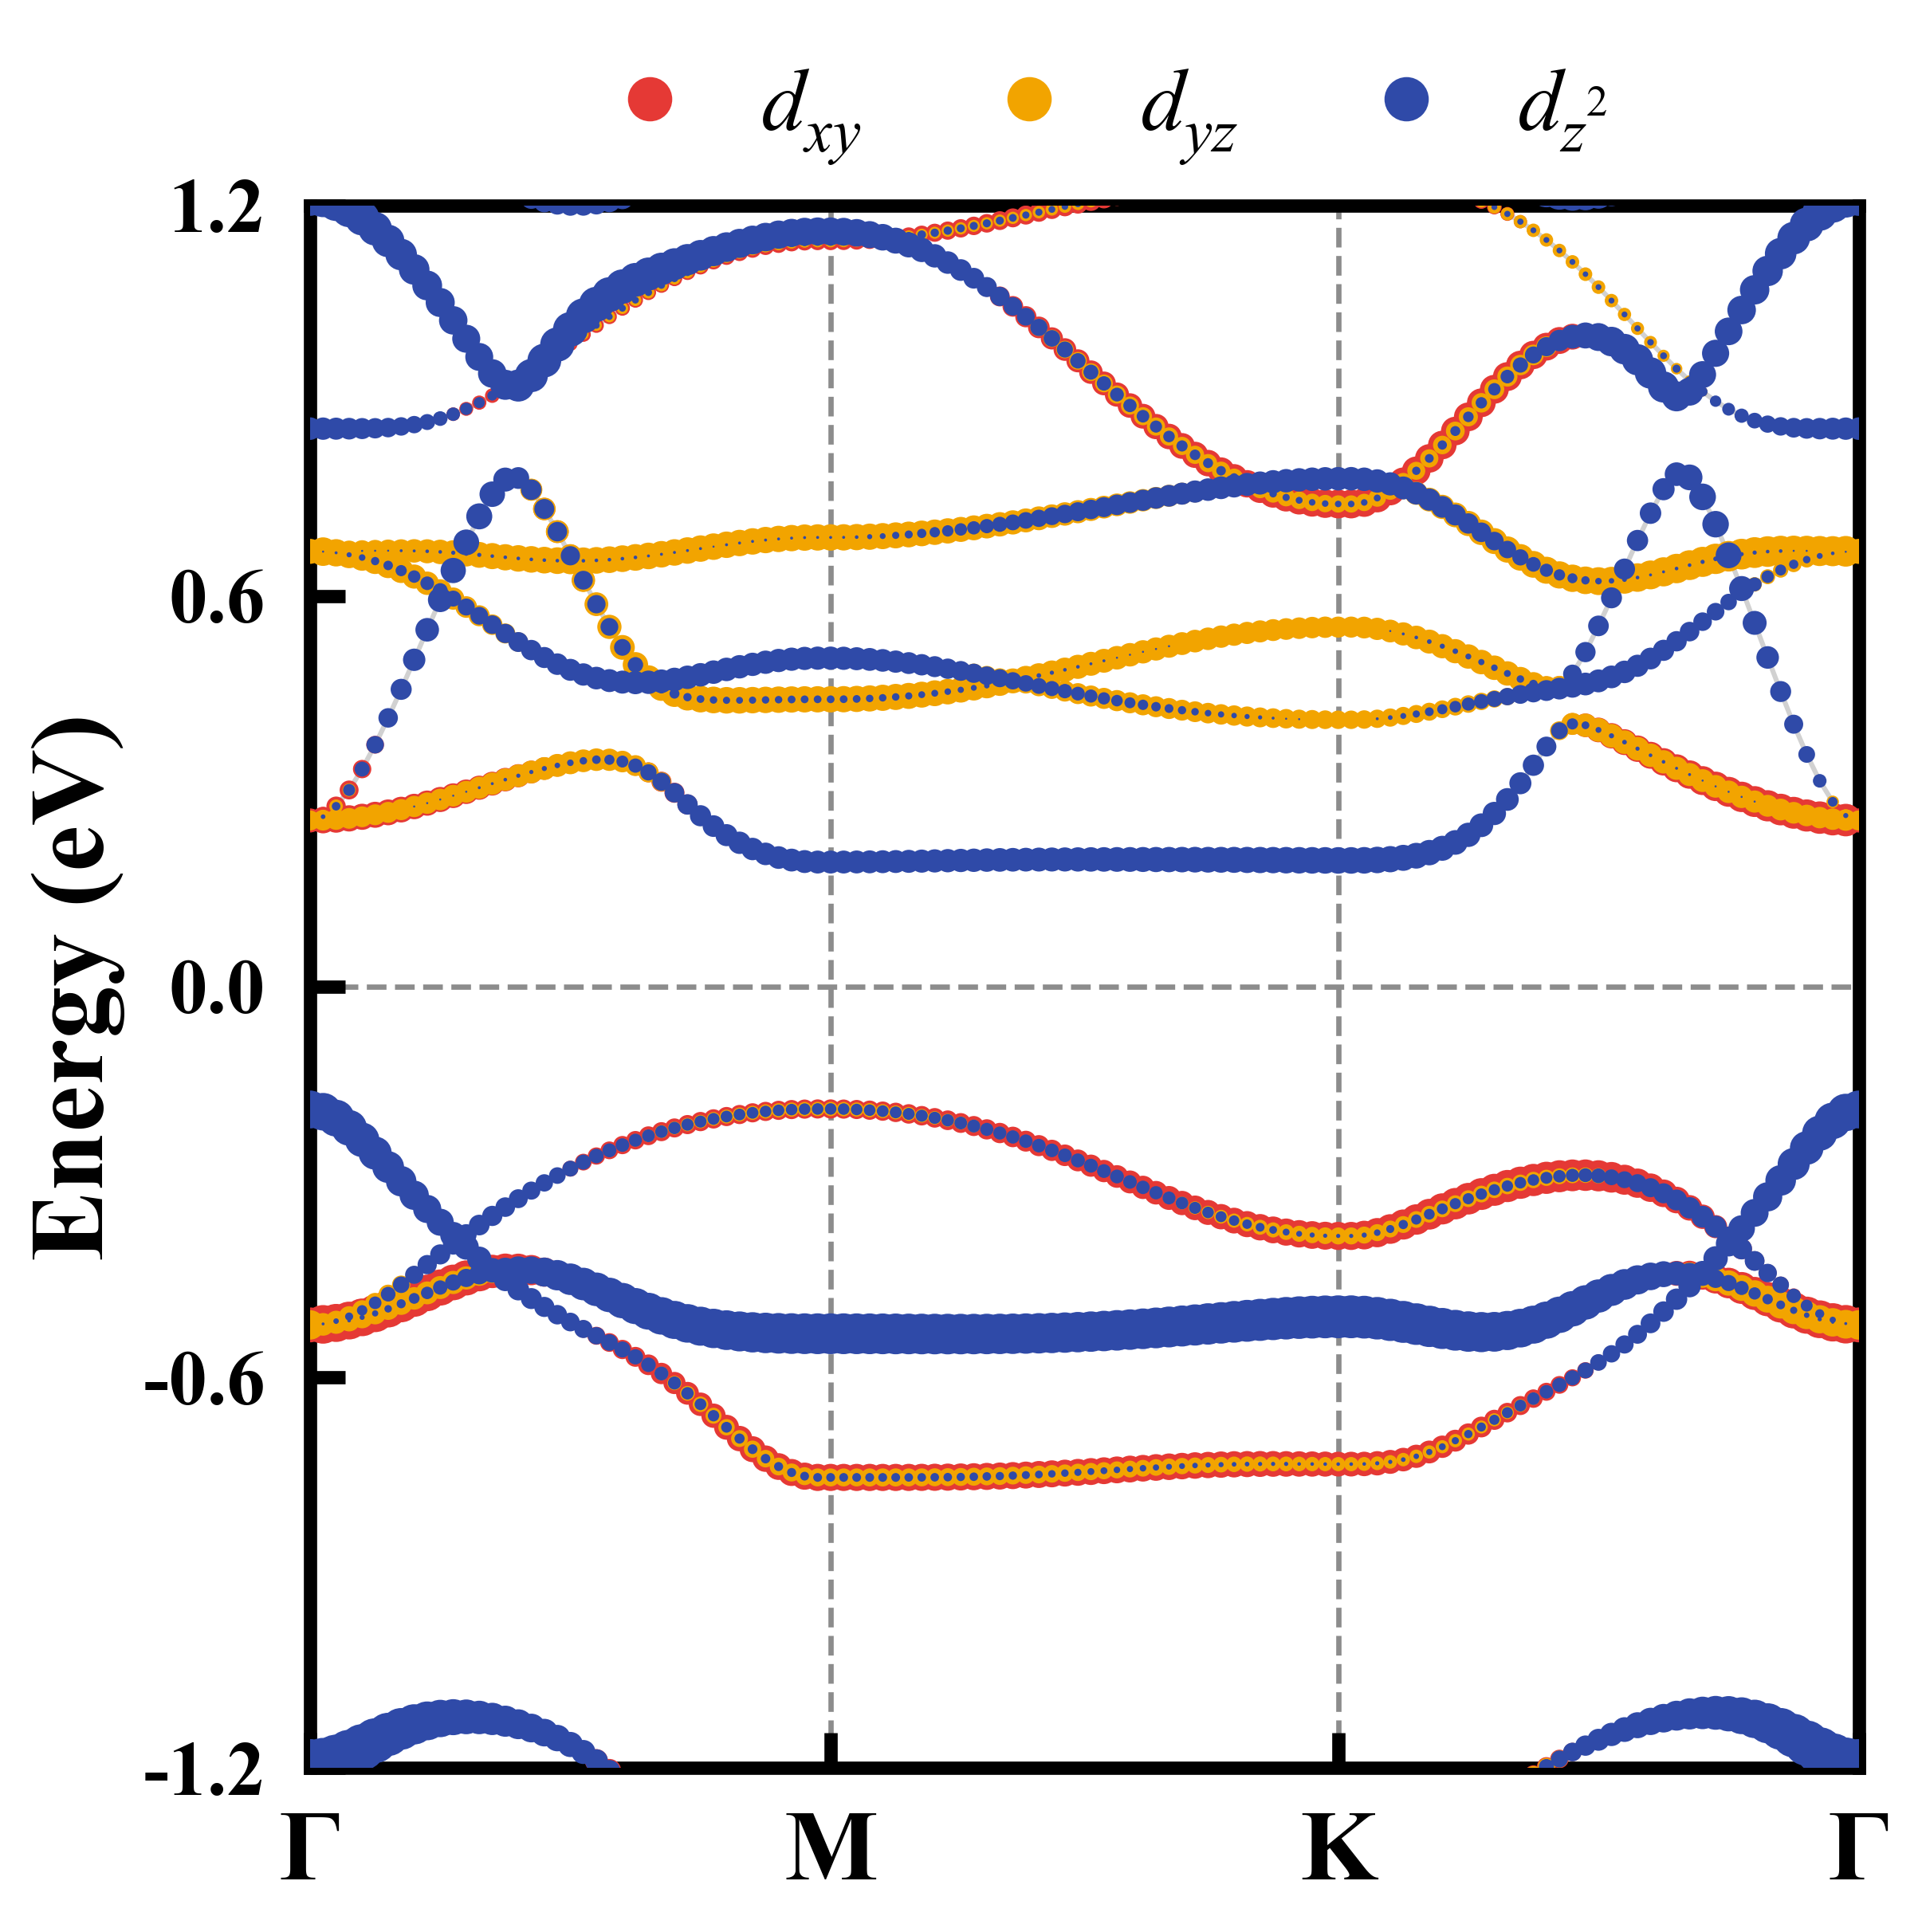
\includegraphics[max width=0.88\linewidth,max height=0.62\textheight,keepaspectratio]{assets/figure-f4be811e7e38.png}
\end{figure}\par\par


2026.3.4补充新代码,考虑soc的时候,上面脚本解析会失败,所以下面版本是绘制考虑soc的投影能带图。\par


\begin{codeindexbox}{代码清单 A.79.8}
语言：python；完整代码见附录第 \pageref{code:79:8} 页，共 522 行。
\end{codeindexbox}


\chapter{拓扑、磁性与三维场可视化}
\begin{partbox}本专题收录 3 篇文章。\end{partbox}

\section{绘制3DMAE的流程(原创脚本与流程)}
\begin{articlemeta}
\textbf{日期：}2025-09-24\hfill\textbf{在线原文：}\href{https://marx2001.github.io/sci-note\_posts/20250924-3DMAE}{marx2001.github.io}
\end{articlemeta}

\subsubsection{3DMAE绘制流程}


\textbf{ 1. 计算3DMAE数据}\par


以MPSS为例,其结构如图所示\par


\par\begin{figure}[H]\centering
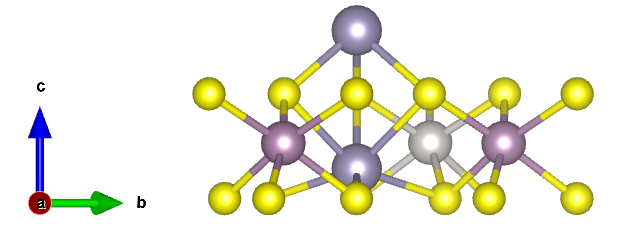
\includegraphics[max width=0.88\linewidth,max height=0.62\textheight,keepaspectratio]{assets/figure-40e35c707e27.png}
\caption{MPSS结构图}
\end{figure}\par


\par\begin{figure}[H]\centering
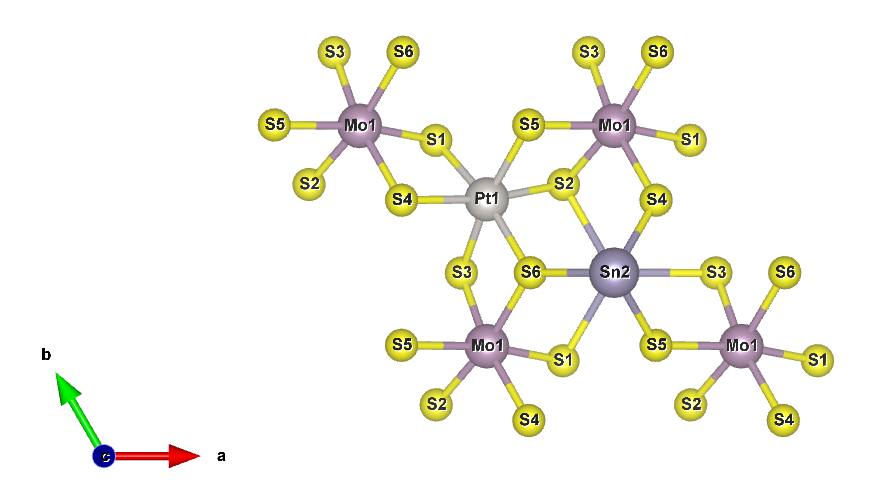
\includegraphics[max width=0.88\linewidth,max height=0.62\textheight,keepaspectratio]{assets/figure-54a09f852c31.png}
\caption{MPSS结构图}
\end{figure}\par


首先,准备输入文件VASPKIT.in文件,POSCAR、POTCAR、KPOINTS、mrx.py以及CHGCAR。\par


VASPKIT.in文件由自己编写,内容如下\par


\begin{codeindexbox}{代码清单 A.80.1}
语言：python；完整代码见附录第 \pageref{code:80:1} 页，共 3 行。
\end{codeindexbox}


INCAR文件如下:\par


\begin{codeindexbox}{代码清单 A.80.2}
语言：python；完整代码见附录第 \pageref{code:80:2} 页，共 37 行。
\end{codeindexbox}


提交计算脚本,脚本内容如下:\par


\begin{codeindexbox}{代码清单 A.80.3}
语言：python；完整代码见附录第 \pageref{code:80:3} 页，共 32 行。
\end{codeindexbox}


\textbf{ 2. 数据后处理与画图}\par


\begin{enumerate}
\item 计算完成后,修改VASPKIT.in文件,将第一行的1改为2,产生MAE.dat数据文件。\par
\item 运行mrx.py,产生四个txt文件\par
\item 打开Origin,同一个系统框内创建四个矩阵。如下图所示,点击画红框的按钮,选择“插入”\par
\end{enumerate}


\par\begin{figure}[H]\centering
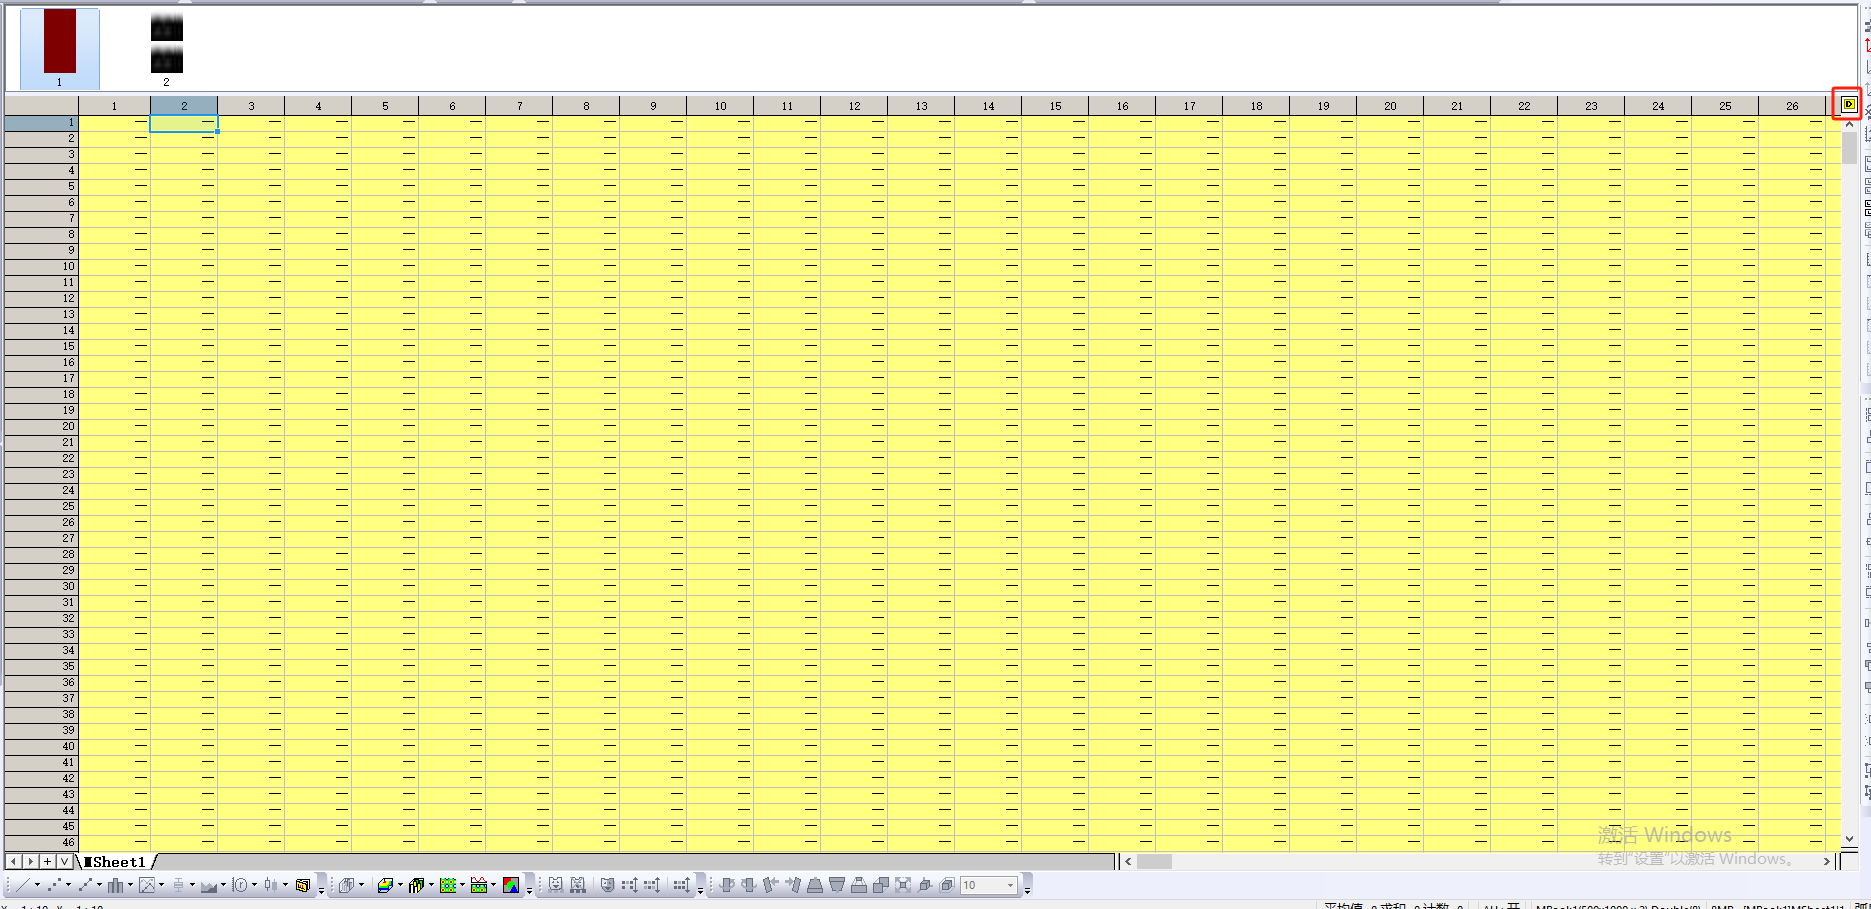
\includegraphics[max width=0.88\linewidth,max height=0.62\textheight,keepaspectratio]{assets/figure-535a98d36d85.png}
\caption{MAE图}
\end{figure}\par


\begin{enumerate}
\item ctrl+A全选,并于工具栏中点击“绘图”-“参数曲面图”,即可产生3DMAE图像。\par
\item 双击页面空白的地方,弹出“图层”框,选择“平面”,将XY、YZ、ZX取消勾选,再旋转到合适的角度,即可得到3DMAE图。如果比例不满意,可以选择“坐标轴”选项,修改某一轴的长度即可找到优美的比例。\par
\end{enumerate}


PS:mrx.py为原创脚本,其代码如下:\par


\begin{codeindexbox}{代码清单 A.80.4}
语言：python；完整代码见附录第 \pageref{code:80:4} 页，共 62 行。
\end{codeindexbox}


也可以用Python进行3DMAE绘图,经过我的精心调试,原创脚本如下:\par


\begin{codeindexbox}{代码清单 A.80.5}
语言：python；完整代码见附录第 \pageref{code:80:5} 页，共 84 行。
\end{codeindexbox}


Python绘图脚本效果如下:\par


\par\begin{figure}[H]\centering
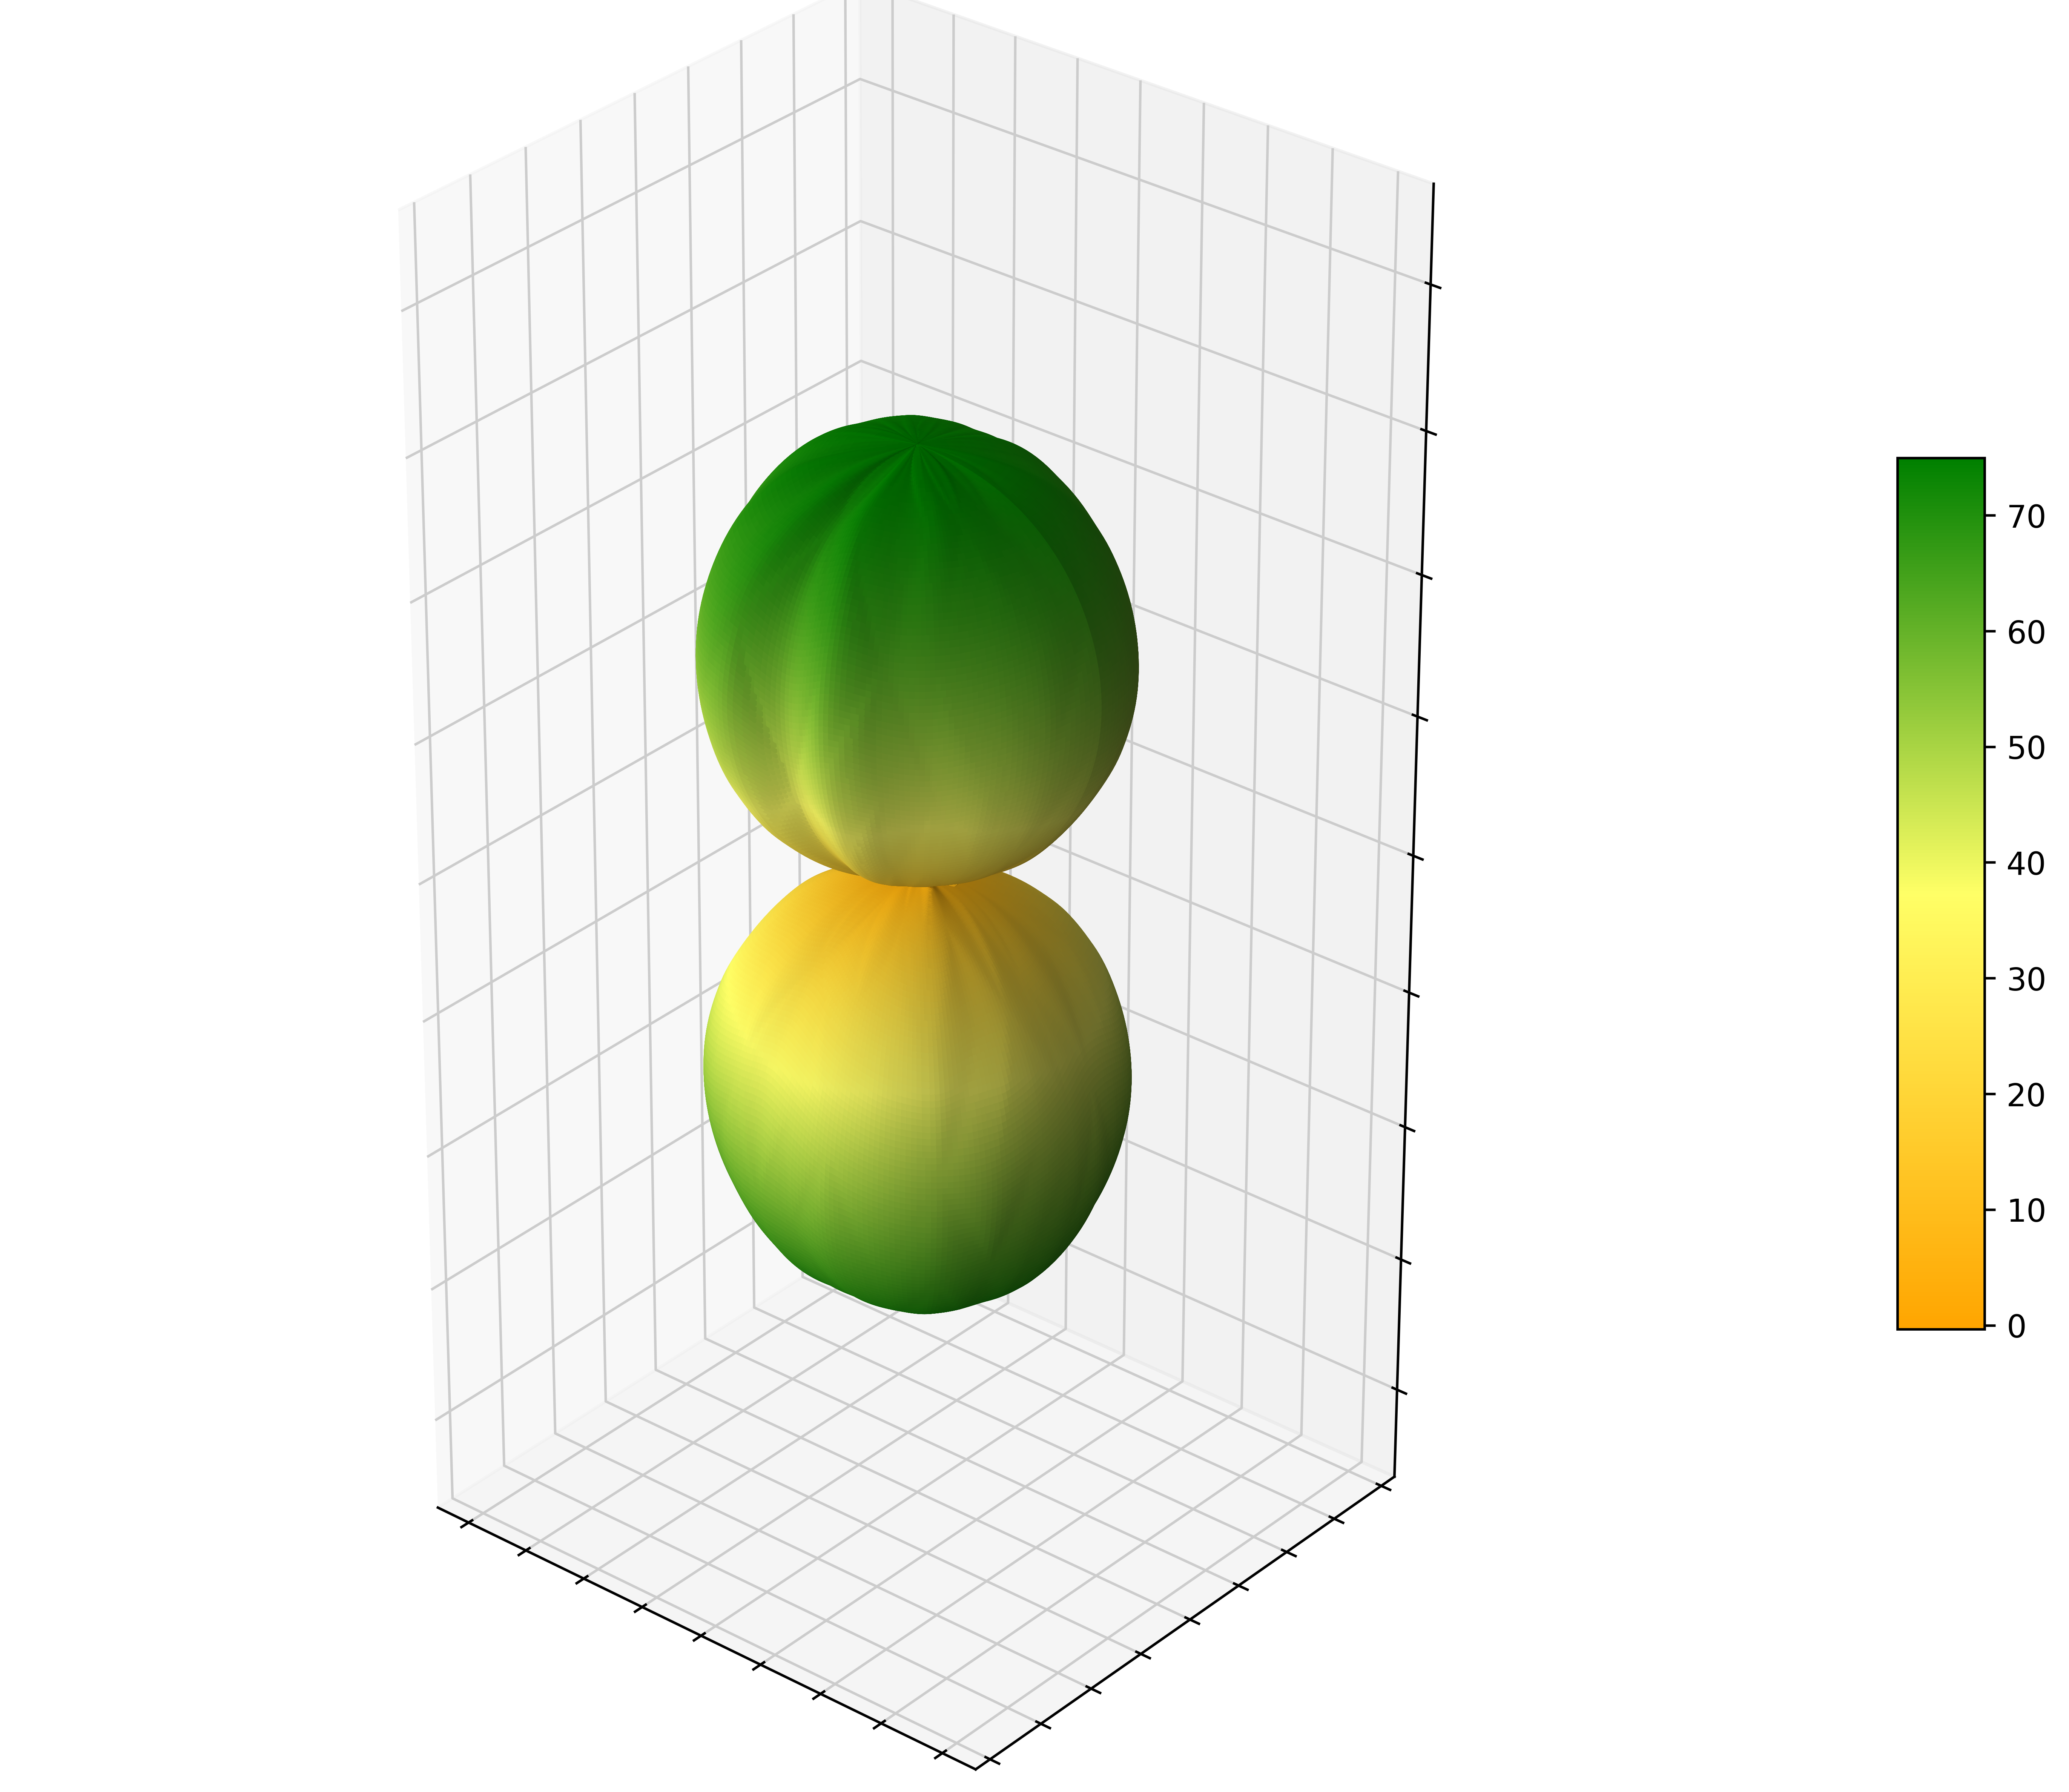
\includegraphics[max width=0.88\linewidth,max height=0.62\textheight,keepaspectratio]{assets/figure-9a5bfaa9f620.png}
\caption{3DMAE图}
\end{figure}\par



\section{vasp绘制自旋密度分布图}
\begin{articlemeta}
\textbf{日期：}2025-10-13\hfill\textbf{在线原文：}\href{https://marx2001.github.io/sci-note\_posts/20251013-picture/}{marx2001.github.io}
\end{articlemeta}

\subsection{用于高通量DMI计算的脚本}


\subsubsection{1.介绍}


简单记录一下如何绘制自旋密度分布图。\par


\subsubsection{2.两种方法}


\begin{enumerate}
\item vtst脚本
\end{enumerate}


命令行输入chgsplit.pl CHGCAR(在静态自洽计算文件夹中),得到CHGCAR\_\allowbreak{}tot、CHGCAR\_\allowbreak{}mag文件\par


放入vesta查看,设置Properties-isosurfaces level=0.023(这个是我的论文中的参考值)or 0.0037\par


\begin{enumerate}
\item vaspkit
\end{enumerate}


vaspkit 312 似乎可以。\par



\section{(原创脚本)vaspberry计算贝里曲率与后处理}
\begin{articlemeta}
\textbf{日期：}2026-03-02\hfill\textbf{在线原文：}\href{https://marx2001.github.io/sci-note\_posts/20260302-berry}{marx2001.github.io}
\end{articlemeta}

\subsubsection{说明}


方法不是原创,后处理程序以及单条能带贝利曲率的计算和细节是原创。\par


原创脚本,盗取必究。\par


\subsubsection{方法}


第一步: VASP的静态计算(要考虑SOC) LWAVE=.TRUE.\par


自洽关键参数:\par


\begin{inlinecodebox}{短代码 · python}
\VerbatimInput[fontsize=\small,breaklines=true,breakanywhere=true,tabsize=2,listparameters={\setlength{\topsep}{0pt}\setlength{\partopsep}{0pt}\setlength{\parsep}{0pt}}]{code/082-001.py}
\end{inlinecodebox}


第二步: 在当前目录提交vaspberry的计算假设我们第一步中的KPOINTS使用的是12 * 12 * 1的参数,价带顶为18,或者我们计算第18个带的贝里曲率以及陈数,则运行命令\par


\begin{codeindexbox}{代码清单 A.82.2}
语言：shell；完整代码见附录第 \pageref{code:82:2} 页，共 1 行。
\end{codeindexbox}


kx和ky是k点数,单层材料ii取1,18是价带顶和导带底分别的序号.此命令为计算第1个带到第18个带的总的贝里曲率以及陈数,而不是单一能带的贝里曲率和陈数。\par


会输出一个贝里曲率的输出文件BERRYCURV.dat 使用自带脚本contour.py,就可以显示贝里曲率了。\par


计算某一条带的贝里曲率和陈数,例如第一占据价带,\par


\begin{codeindexbox}{代码清单 A.82.3}
语言：shell；完整代码见附录第 \pageref{code:82:3} 页，共 1 行。
\end{codeindexbox}


若自洽为共线计算(vasp\_\allowbreak{}std),则在vaspberry所在目录将自洽计算的波函数WAVECAR拷贝进来,运行:\par


\begin{codeindexbox}{代码清单 A.82.4}
语言：shell；完整代码见附录第 \pageref{code:82:4} 页，共 1 行。
\end{codeindexbox}


注意kx 和 ky值要与KPOINTS k点个数一致,-s 1表示共线计算,18表示价带顶.\par


改进版后处理代码(原创):\par


\begin{codeindexbox}{代码清单 A.82.5}
语言：python；完整代码见附录第 \pageref{code:82:5} 页，共 55 行。
\end{codeindexbox}


第二个版本:\par


\begin{codeindexbox}{代码清单 A.82.6}
语言：python；完整代码见附录第 \pageref{code:82:6} 页，共 57 行。
\end{codeindexbox}


绘图则放到ppt内另行处理。选择ppt内图片格式中的矫正颜色,让对比度增加20\%,也可以进行其他处理。\par


我自己的计算命令:\par


\begin{codeindexbox}{代码清单 A.82.7}
语言：shell；完整代码见附录第 \pageref{code:82:7} 页，共 1 行。
\end{codeindexbox}


计算单带贝利曲率,原创代码:\par


创建ipynb文件\par


cell1:\par


\begin{codeindexbox}{代码清单 A.82.8}
语言：python；完整代码见附录第 \pageref{code:82:8} 页，共 24 行。
\end{codeindexbox}


cell2:\par


\begin{codeindexbox}{代码清单 A.82.9}
语言：python；完整代码见附录第 \pageref{code:82:9} 页，共 12 行。
\end{codeindexbox}


cell3\par


\begin{codeindexbox}{代码清单 A.82.10}
语言：python；完整代码见附录第 \pageref{code:82:10} 页，共 19 行。
\end{codeindexbox}


cell4\par


\begin{codeindexbox}{代码清单 A.82.11}
语言：python；完整代码见附录第 \pageref{code:82:11} 页，共 8 行。
\end{codeindexbox}


cell5\par


\begin{codeindexbox}{代码清单 A.82.12}
语言：python；完整代码见附录第 \pageref{code:82:12} 页，共 228 行。
\end{codeindexbox}


这个脚本会生成一个dat文件,第一列和第五列是我们放到origin绘图的数据,分别是x和y轴。\par


增大取点N\_\allowbreak{}PER\_\allowbreak{}SEG = 3,设置费米能级EF = -1.4862,修改价带和导带编号,脚本默认计算全部的价带+n条导带:\par


\begin{inlinecodebox}{短代码 · python}
\VerbatimInput[fontsize=\small,breaklines=true,breakanywhere=true,tabsize=2,listparameters={\setlength{\topsep}{0pt}\setlength{\partopsep}{0pt}\setlength{\parsep}{0pt}}]{code/082-013.py}
\end{inlinecodebox}


20260303更新代码方便绘图:\par


新增两个cell:\par


\begin{codeindexbox}{代码清单 A.82.14}
语言：python；完整代码见附录第 \pageref{code:82:14} 页，共 44 行。
\end{codeindexbox}


上面的cell用于,输出当前使用的高对称点,下面的cell把高对称点作为横轴,贝利曲率作为y轴,绘制1D折线图,并输出一个名叫final.dat的数据文件。\par


\begin{codeindexbox}{代码清单 A.82.15}
语言：python；完整代码见附录第 \pageref{code:82:15} 页，共 61 行。
\end{codeindexbox}


x轴用第一列,y轴用Omega\_\allowbreak{}xy这一列。\par


再次更新一个cell,用于输出高对称带点\par


\begin{codeindexbox}{代码清单 A.82.16}
语言：python；完整代码见附录第 \pageref{code:82:16} 页，共 27 行。
\end{codeindexbox}


再次更新,可以用于论文的绘图代码,新的cell基于已经计算好的数据进行绘图:\par


\begin{codeindexbox}{代码清单 A.82.17}
语言：python；完整代码见附录第 \pageref{code:82:17} 页，共 176 行。
\end{codeindexbox}


上面是绘制全部价带的贝利曲率分布图,下方给出考虑导带数目后的贝利曲率分布折线图:\par


作为ipynb文件的cell写入\par


\begin{codeindexbox}{代码清单 A.82.18}
语言：python；完整代码见附录第 \pageref{code:82:18} 页，共 54 行。
\end{codeindexbox}


如果数值过大,则不需要单位转换直接用下方代码生成贝利曲率图片:\par


\begin{codeindexbox}{代码清单 A.82.19}
语言：python；完整代码见附录第 \pageref{code:82:19} 页，共 176 行。
\end{codeindexbox}


原创脚本,盗取必究。\par


\chapter{结构建模与三维渲染}
\begin{partbox}本专题收录 2 篇文章。\end{partbox}

\section{(原创脚本)blender绘制斯格明子}
\begin{articlemeta}
\textbf{日期：}2026-03-07\hfill\textbf{在线原文：}\href{https://marx2001.github.io/sci-note\_posts/20260307-blender}{marx2001.github.io}
\end{articlemeta}

\subsubsection{说明}


均为原创,禁止抄袭,转载注明出处,否则必会追究。\par


\subsubsection{方法}


(1) 原子自旋模拟,提交spirit任务得到ovf文件。\par


(2) 收集所有的ovf文件,并转换成图片,脚本如下:\par


sh脚本负责收集,python负责绘制,配色为原创:\par


\begin{codeindexbox}{代码清单 A.83.1}
语言：shell；完整代码见附录第 \pageref{code:83:1} 页，共 9 行。
\end{codeindexbox}


\begin{codeindexbox}{代码清单 A.83.2}
语言：python；完整代码见附录第 \pageref{code:83:2} 页，共 127 行。
\end{codeindexbox}


(3) 筛选需要绘制的ovf文件和对应的图片。复制到同一个文件夹中\par


(4) 先将ovf转换为csv文件,记录自旋数据,这是一个ipynb文件,需要opencv库。改晶格常数等信息。\par


\begin{codeindexbox}{代码清单 A.83.3}
语言：python；完整代码见附录第 \pageref{code:83:3} 页，共 162 行。
\end{codeindexbox}


(5) 框选想要绘制的区域。\par


\begin{codeindexbox}{代码清单 A.83.4}
语言：python；完整代码见附录第 \pageref{code:83:4} 页，共 69 行。
\end{codeindexbox}


(6) 记录上一步输出的 ROI 参数,据此计算目标绘制区域的坐标,同时修改相应的 PNG 和 CSV 文件名。\par


\begin{codeindexbox}{代码清单 A.83.5}
语言：shell；完整代码见附录第 \pageref{code:83:5} 页，共 1 行。
\end{codeindexbox}


将坐标填入下方脚本\par


\begin{codeindexbox}{代码清单 A.83.6}
语言：python；完整代码见附录第 \pageref{code:83:6} 页，共 42 行。
\end{codeindexbox}


(7)转换xywh坐标为xyz坐标,即将图片中的位置转换为csv文件的位置。\par


\begin{codeindexbox}{代码清单 A.83.7}
语言：python；完整代码见附录第 \pageref{code:83:7} 页，共 42 行。
\end{codeindexbox}


(8)上一个脚本的输出如下所示,填入到下一个脚本结尾的相应的xyz坐标处:\par


\begin{codeindexbox}{代码清单 A.83.8}
语言：shell；完整代码见附录第 \pageref{code:83:8} 页，共 4 行。
\end{codeindexbox}


\begin{codeindexbox}{代码清单 A.83.9}
语言：python；完整代码见附录第 \pageref{code:83:9} 页，共 48 行。
\end{codeindexbox}


(9)计算切割后的斯格明子的自旋数据并形成spin texture图,观察是否是自己想要的那一个区域。\par


\begin{codeindexbox}{代码清单 A.83.10}
语言：python；完整代码见附录第 \pageref{code:83:10} 页，共 44 行。
\end{codeindexbox}


(10) 以下为 Blender 代码。需将 Blender 工程文件与上述输出文件置于同一文件夹。\par


这个是抠图版的代码,只绘制斯格明子本身\par


\begin{codeindexbox}{代码清单 A.83.11}
语言：python；完整代码见附录第 \pageref{code:83:11} 页，共 44 行。
\end{codeindexbox}


这个是方形的背景\par


\begin{codeindexbox}{代码清单 A.83.12}
语言：python；完整代码见附录第 \pageref{code:83:12} 页，共 44 行。
\end{codeindexbox}


上面是绘制ovf到blender的全部流程,后面会记录如何自己创建一个自旋数据csv文件,并用blender绘制出来。\par



\section{(绘图教程) VESTA 到 Blender 的二维材料3D论文原子结构绘图教程}
\begin{articlemeta}
\textbf{日期：}2026-09-04\hfill\textbf{在线原文：}\href{https://marx2001.github.io/sci-note\_posts/20260904-vesta-blender}{marx2001.github.io}
\end{articlemeta}

\#\#\par


\begin{codeindexbox}{代码清单 A.84.1}
语言：text；完整代码见附录第 \pageref{code:84:1} 页，共 1 行。
\end{codeindexbox}


说明\par


\begin{codeindexbox}{代码清单 A.84.2}
语言：text；完整代码见附录第 \pageref{code:84:2} 页，共 1 行。
\end{codeindexbox}


本文记录如何将第一性原理计算得到的晶体结构文件,通过 \textbf{VESTA → Blender} 转换为适用于论文 Figure 的三维原子结构模型。\par


该流程面向没有 Blender 使用经验的科研人员,目标是:\par


\begin{codeindexbox}{代码清单 A.84.3}
语言：text；完整代码见附录第 \pageref{code:84:3} 页，共 9 行。
\end{codeindexbox}


核心思想:\par


\begin{codeindexbox}{代码清单 A.84.4}
语言：text；完整代码见附录第 \pageref{code:84:4} 页，共 2 行。
\end{codeindexbox}


不要直接在 Blender 中手动搭建晶体结构。对于二维材料和异质结构,原子坐标、键连接和周期性必须由晶体软件保证。\par


\medskip\hrule\medskip


\subsection{一、整体工作流概览}


\subsubsection{Step 1:准备结构文件}


输入文件:\par


\begin{codeindexbox}{代码清单 A.84.5}
语言：text；完整代码见附录第 \pageref{code:84:5} 页，共 3 行。
\end{codeindexbox}


推荐使用:\par


\begin{codeindexbox}{代码清单 A.84.6}
语言：text；完整代码见附录第 \pageref{code:84:6} 页，共 1 行。
\end{codeindexbox}


原因:\par


\begin{itemize}
\item 已经过结构优化;
\item 原子位置更加稳定;
\item 可直接用于论文结构展示。
\end{itemize}


\medskip\hrule\medskip


\subsubsection{Step 2:VESTA处理结构}


VESTA主要完成:\par


\begin{codeindexbox}{代码清单 A.84.7}
语言：text；完整代码见附录第 \pageref{code:84:7} 页，共 11 行。
\end{codeindexbox}


VESTA不建议作为最终渲染工具,而作为结构准备工具。\par


\medskip\hrule\medskip


\subsection{二、VESTA结构处理步骤}


\subsubsection{1. 导入结构}


打开:\par


\begin{codeindexbox}{代码清单 A.84.8}
语言：text；完整代码见附录第 \pageref{code:84:8} 页，共 1 行。
\end{codeindexbox}


加载:\par


\begin{codeindexbox}{代码清单 A.84.9}
语言：text；完整代码见附录第 \pageref{code:84:9} 页，共 1 行。
\end{codeindexbox}


检查:\par


\begin{itemize}
\item 元素种类;
\item 原子数量;
\item 晶格参数;
\item 层间结构。
\end{itemize}


\medskip\hrule\medskip


\subsubsection{2. 扩胞}


二维材料通常需要扩胞显示周期性。\par


路径:\par


\begin{codeindexbox}{代码清单 A.84.10}
语言：text；完整代码见附录第 \pageref{code:84:10} 页，共 5 行。
\end{codeindexbox}


设置:\par


例如:\par


\begin{inlinecodebox}{短代码 · text}
\VerbatimInput[fontsize=\small,breaklines=true,breakanywhere=true,tabsize=2,listparameters={\setlength{\topsep}{0pt}\setlength{\partopsep}{0pt}\setlength{\parsep}{0pt}}]{code/084-011.txt}
\end{inlinecodebox}


得到:\par


\begin{codeindexbox}{代码清单 A.84.12}
语言：text；完整代码见附录第 \pageref{code:84:12} 页，共 1 行。
\end{codeindexbox}


注意:\par


不要在 Blender 中直接扩胞。\par


原因:\par


\begin{itemize}
\item 周期关系难以控制;
\item 键连接容易错误;
\item 模型容易出现断键。
\end{itemize}


\medskip\hrule\medskip


\subsubsection{3. 设置原子和键}


建议:\par


显示主要化学键:\par


例如:\par


\begin{codeindexbox}{代码清单 A.84.13}
语言：text；完整代码见附录第 \pageref{code:84:13} 页，共 2 行。
\end{codeindexbox}


关闭不必要连接:\par


例如:\par


\begin{codeindexbox}{代码清单 A.84.14}
语言：text；完整代码见附录第 \pageref{code:84:14} 页，共 1 行。
\end{codeindexbox}


原则:\par


结构展示不是显示所有可能连接,而是突出晶体骨架。\par


\medskip\hrule\medskip


\subsubsection{4. 调整原子比例}


VESTA默认原子大小通常偏小。\par


论文图建议:\par


\begin{itemize}
\item 磁性元素适当放大;
\item 配位原子保持比例;
\item 键不要过粗。
\end{itemize}


\medskip\hrule\medskip


\subsection{三、VESTA导出到Blender}


\subsubsection{推荐路线}


\begin{codeindexbox}{代码清单 A.84.15}
语言：text；完整代码见附录第 \pageref{code:84:15} 页，共 5 行。
\end{codeindexbox}


原因:\par


VRML可以保留:\par


\begin{itemize}
\item 原子球;
\item 键;
\item 基本颜色信息。
\end{itemize}


\medskip\hrule\medskip


导出:\par


\begin{codeindexbox}{代码清单 A.84.16}
语言：text；完整代码见附录第 \pageref{code:84:16} 页，共 5 行。
\end{codeindexbox}


得到:\par


\begin{codeindexbox}{代码清单 A.84.17}
语言：text；完整代码见附录第 \pageref{code:84:17} 页，共 1 行。
\end{codeindexbox}


\medskip\hrule\medskip


\subsection{四、Blender导入流程(新手)}


\subsubsection{Step 1:安装VRML导入插件}


Blender 4.2默认可能没有VRML导入。\par


进入:\par


\begin{codeindexbox}{代码清单 A.84.18}
语言：text；完整代码见附录第 \pageref{code:84:18} 页，共 5 行。
\end{codeindexbox}


搜索:\par


\begin{codeindexbox}{代码清单 A.84.19}
语言：text；完整代码见附录第 \pageref{code:84:19} 页，共 1 行。
\end{codeindexbox}


如果没有:\par


需要安装支持VRML/\allowbreak{}Web3D格式的插件。\par


\medskip\hrule\medskip


\subsubsection{Step 2:导入结构}


菜单:\par


\begin{codeindexbox}{代码清单 A.84.20}
语言：text；完整代码见附录第 \pageref{code:84:20} 页，共 5 行。
\end{codeindexbox}


选择:\par


\begin{codeindexbox}{代码清单 A.84.21}
语言：text；完整代码见附录第 \pageref{code:84:21} 页，共 1 行。
\end{codeindexbox}


导入后:\par


模型会出现:\par


\begin{itemize}
\item 原子球;
\item 键柱;
\item 材质。
\end{itemize}


\medskip\hrule\medskip


\subsection{五、Blender论文级调整流程}


\subsubsection{1. 设置Camera}


不要直接使用默认Camera。\par


推荐:\par


\begin{codeindexbox}{代码清单 A.84.22}
语言：text；完整代码见附录第 \pageref{code:84:22} 页，共 5 行。
\end{codeindexbox}


将当前视角绑定给Camera。\par


\medskip\hrule\medskip


\subsubsection{2. Camera参数建议}


二维异质结构推荐:\par


\begin{codeindexbox}{代码清单 A.84.23}
语言：text；完整代码见附录第 \pageref{code:84:23} 页，共 2 行。
\end{codeindexbox}


如果结构被裁剪:\par


降低焦距:\par


例如:\par


\begin{codeindexbox}{代码清单 A.84.24}
语言：text；完整代码见附录第 \pageref{code:84:24} 页，共 1 行。
\end{codeindexbox}


\medskip\hrule\medskip


\subsubsection{3. 画幅设置}


横向二维材料推荐:\par


\begin{codeindexbox}{代码清单 A.84.25}
语言：text；完整代码见附录第 \pageref{code:84:25} 页，共 1 行。
\end{codeindexbox}


或者:\par


\begin{codeindexbox}{代码清单 A.84.26}
语言：text；完整代码见附录第 \pageref{code:84:26} 页，共 1 行。
\end{codeindexbox}


比例:\par


约2:1。\par


\medskip\hrule\medskip


\subsection{六、常见问题与解决方法}


\subsubsection{问题1:渲染结果缺少一半结构}


原因:\par


Camera视野太小。\par


解决:\par


检查:\par


\begin{codeindexbox}{代码清单 A.84.27}
语言：text；完整代码见附录第 \pageref{code:84:27} 页，共 1 行。
\end{codeindexbox}


降低:\par


\begin{codeindexbox}{代码清单 A.84.28}
语言：text；完整代码见附录第 \pageref{code:84:28} 页，共 1 行。
\end{codeindexbox}


或者:\par


增大Camera距离。\par


\medskip\hrule\medskip


\subsubsection{问题2:Viewport视角和Camera视角不同}


原因:\par


Viewport不是Camera。\par


解决:\par


当前满意视角:\par


执行:\par


\begin{codeindexbox}{代码清单 A.84.29}
语言：text；完整代码见附录第 \pageref{code:84:29} 页，共 1 行。
\end{codeindexbox}


或者:\par


\begin{codeindexbox}{代码清单 A.84.30}
语言：text；完整代码见附录第 \pageref{code:84:30} 页，共 5 行。
\end{codeindexbox}


\medskip\hrule\medskip


\subsubsection{问题3:原子之间键断裂}


原因:\par


键长阈值设置错误。\par


解决:\par


在VESTA重新设置bond距离。\par


不要在Blender中手动连接大量键。\par


\medskip\hrule\medskip


\subsubsection{问题4:结构颜色灰暗,没有质感}


原因:\par


Blender默认材质和VESTA不同。\par


解决:\par


调整:\par


\subsubsection{Color Management}


推荐:\par


\begin{codeindexbox}{代码清单 A.84.31}
语言：text；完整代码见附录第 \pageref{code:84:31} 页，共 2 行。
\end{codeindexbox}


增加:\par


\begin{codeindexbox}{代码清单 A.84.32}
语言：text；完整代码见附录第 \pageref{code:84:32} 页，共 2 行。
\end{codeindexbox}


\medskip\hrule\medskip


\subsubsection{问题5:结构过于稀疏}


原因:\par


\begin{itemize}
\item 原子半径过小;
\item 键过细。
\end{itemize}


解决:\par


增加:\par


\begin{codeindexbox}{代码清单 A.84.33}
语言：text；完整代码见附录第 \pageref{code:84:33} 页，共 2 行。
\end{codeindexbox}


增加:\par


\begin{codeindexbox}{代码清单 A.84.34}
语言：text；完整代码见附录第 \pageref{code:84:34} 页，共 2 行。
\end{codeindexbox}


\medskip\hrule\medskip


\subsubsection{问题6:没有VESTA的球体质感}


原因:\par


VESTA采用简单Phong光照,而Blender使用PBR材质。\par


解决:\par


Blender中:\par


降低Metallic:\par


\begin{codeindexbox}{代码清单 A.84.35}
语言：text；完整代码见附录第 \pageref{code:84:35} 页，共 1 行。
\end{codeindexbox}


调整:\par


\begin{codeindexbox}{代码清单 A.84.36}
语言：text；完整代码见附录第 \pageref{code:84:36} 页，共 2 行。
\end{codeindexbox}


增加Specular效果。\par


\medskip\hrule\medskip


\subsection{七、推荐Blender渲染设置}


\subsubsection{材质原则}


原子不要设置为金属。\par


推荐:\par


\begin{codeindexbox}{代码清单 A.84.37}
语言：text；完整代码见附录第 \pageref{code:84:37} 页，共 5 行。
\end{codeindexbox}


类似VESTA的塑料球效果。\par


\medskip\hrule\medskip


\subsubsection{灯光}


推荐三点布光:\par


\begin{codeindexbox}{代码清单 A.84.38}
语言：text；完整代码见附录第 \pageref{code:84:38} 页，共 8 行。
\end{codeindexbox}


或者:\par


一个大面积Area Light + 环境光。\par


\medskip\hrule\medskip


\subsection{八、最终推荐流程总结}


\begin{codeindexbox}{代码清单 A.84.39}
语言：text；完整代码见附录第 \pageref{code:84:39} 页，共 21 行。
\end{codeindexbox}


\medskip\hrule\medskip


\subsection{九、最终原则}


\begin{codeindexbox}{代码清单 A.84.40}
语言：text；完整代码见附录第 \pageref{code:84:40} 页，共 8 行。
\end{codeindexbox}


对于二维磁性异质结构:\par


推荐采用:\par


\begin{codeindexbox}{代码清单 A.84.41}
语言：text；完整代码见附录第 \pageref{code:84:41} 页，共 1 行。
\end{codeindexbox}


作为论文 Figure 制作流程。\par


\part{心得笔记}
\chapter{计算调试与方法反思}
\begin{partbox}集中收录复现体会、计算调试、方法反思与阶段性研究总结,展示研究问题如何被发现、分析和修正。\par\medskip 本专题收录 6 篇文章。\end{partbox}

\section{复现文献中材料结构的心得}
\begin{articlemeta}
\textbf{日期：}2025-10-11\hfill\textbf{在线原文：}\href{https://marx2001.github.io/sci-note\_posts/20251011-F}{marx2001.github.io}
\end{articlemeta}

\subsection{摘要}


为了寻找合适的作为多铁异质结铁磁层的材料,准备复现一篇文献,VSeTe具有铁谷性和铁磁性,可以作为候选材料。\par


异质结结构优化心得体会。\par


本次最大收获是发现了一个复现文献结构的新思路——AI辅助法,即通过输入文献中关于结构的描述到AI中,然后让它根据格子的种类,换算成分数坐标,形成POSCAR,这样,键长、键角可以完美的与文献匹配。\par


\textbf{ 1. Janus单层复现文献的心得体会}\par


复现文献结构是一个最大的问题,结构不对,基本上所有的性质都不能和文献匹配,因此得到一个正确的结构是一个艰巨的任务,今天上午,历经3个小时20分钟,终于得到了一个与文献一致的结构。下面是我的复现过程与心得体会\par


首先,我选择之前复现过二维铁磁半导体Janus材料的H-CrSeBr的POSCAR作为起始文件,替换POSCAR中的元素,即可得到H-VSeTe单层的初始结构,然后开始结构优化,不加磁性。我发现,并不能得到正确的结构,最多 是得到相近的结构\par


然后我通过固定ISIF=2,控制晶格常数不变,继续优化,但始终优化不到正确的构型中去,因此想开辟新思路,让AI写代码辅助,具体的过程如开头所示。代码如下:\par


\begin{codeindexbox}{代码清单 A.85.1}
语言：python；完整代码见附录第 \pageref{code:85:1} 页，共 196 行。
\end{codeindexbox}


虽然这个脚本比较呆板,但也是解决了我当下的问题。\par


获得文献结构的另一种方法,是寻找这个结构的原始构型,可以询问AI或者找综述文献,比如TiCdO4,市面上的两篇文献均未提供材料的晶格常数等信息,但是这个材料是TiO2演变而来。\par


\textbf{ 2. 异质结结构优化的心得体会}\par


异质结结构优化是一个巨大的问题,因为漫长且充满了不确定性——畸变随时可能发生。我做了MnSeTe和拓扑绝缘体VTeCl与Zr2Ge2Te6的异质结,晶格失配率约为0.05\%。其结构优化共同的问题是,会发生严重的畸变,变成1T’相的Janus结构。\par


ISIF=2和ISIF=3的结构优化均不能解决该问题。大概只能通过寻找不畸变的异质结才能解决问题。上述两种异质结畸变之后,由半导体变为金属,性质变化剧烈且并无特殊性质出现。\par



\section{vasp结构优化}
\begin{articlemeta}
\textbf{日期：}2025-10-14\hfill\textbf{在线原文：}\href{https://marx2001.github.io/sci-note\_posts/20250926-geo2}{marx2001.github.io}
\end{articlemeta}

\subsection{摘要}


相比于2025.9.26以类似名称命名的文章中的结构优化方式,本人今天继续记录一下最近一周的对于结构优化的心得体会。本文提出了一种最严谨的结构优化方式,然后基于我的想法,我去寻找了文献,以此证明我的理论 的正确性(看到论文后,感叹我真是晚生了几十年,早生几年这文章我自己就发了)。\par


\subsubsection{1. 详细步骤}


首先,对于强关联体系(过渡金属元素,重元素),需要进行DFT+U,这个是众所周知的,但是对于结构优化过程中是否需要加U,很多人并不清楚,做第一性原理计算的时候也并不严谨,包括我目前的课题组内的所有成员,包括已经去各个985读博的所有人,大概率或者百分百没有按照严谨的流程进行结构优化。\par



\section{单层和滑移的系数推导结果}
\begin{articlemeta}
\textbf{日期：}2025-11-21\hfill\textbf{在线原文：}\href{https://marx2001.github.io/sci-note\_posts/20251121-m}{marx2001.github.io}
\end{articlemeta}

\subsubsection{心得笔记}


\subsubsection{2025.11.21 总结}


单层的系数:\par


16,16,16,1 -16,16,16,1 0,0,16,1 0,8,0,1\par


滑移的系数 32,32,32,32,64,1 32,32,32,-32,-64,1 16,16,0,0,0,1 -32,32,32,0,0,1 0 ,32 ,32,0,0,1 16,0 ,32 ,0, 0, 1\par


对应的磁态后续整理\par



\section{VASP计算出的磁参数的归一化问题}
\begin{articlemeta}
\textbf{日期：}2025-11-26\hfill\textbf{在线原文：}\href{https://marx2001.github.io/sci-note\_posts/20251126-if}{marx2001.github.io}
\end{articlemeta}

\subsection{Answer}


\par\begin{figure}[H]\centering
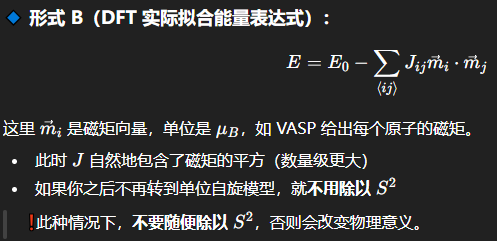
\includegraphics[max width=0.88\linewidth,max height=0.62\textheight,keepaspectratio]{assets/figure-094d146be497.png}
\end{figure}\par\par


\par\begin{figure}[H]\centering
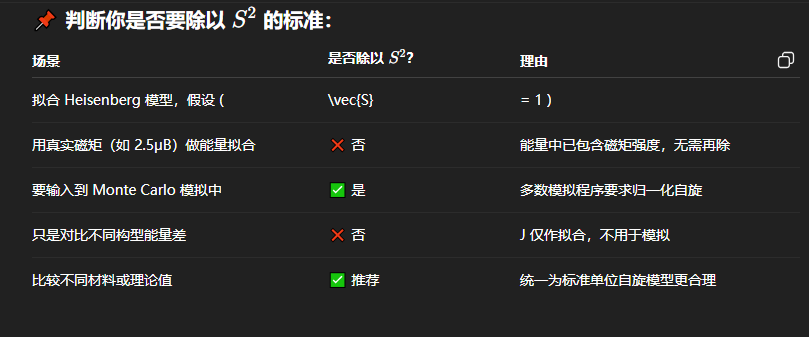
\includegraphics[max width=0.88\linewidth,max height=0.62\textheight,keepaspectratio]{assets/figure-cb367161a90e.png}
\end{figure}\par\par



\section{异常DMI的数值调试}
\begin{articlemeta}
\textbf{日期：}2025-11-26\hfill\textbf{在线原文：}\href{https://marx2001.github.io/sci-note\_posts/20251126-x}{marx2001.github.io}
\end{articlemeta}

\subsubsection{心得笔记}


\subsubsection{异常DMI的数值与日志}


增大RWIGS会导致DMI增大,RWIGS=1.27→1.5\par


\subsubsection{wannier90日志}


k点取5 5 1的时候,ncl的static顺利收敛, 但是增大k点到21 21 1的时候,不收敛\par


\subsubsection{笔记}


\par\begin{figure}[H]\centering
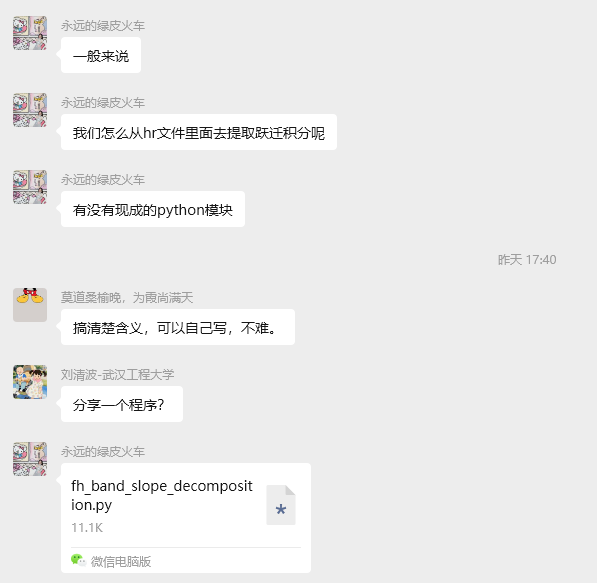
\includegraphics[max width=0.88\linewidth,max height=0.62\textheight,keepaspectratio]{assets/figure-b96fa9cfb0cc.png}
\end{figure}\par\par


\par\begin{figure}[H]\centering
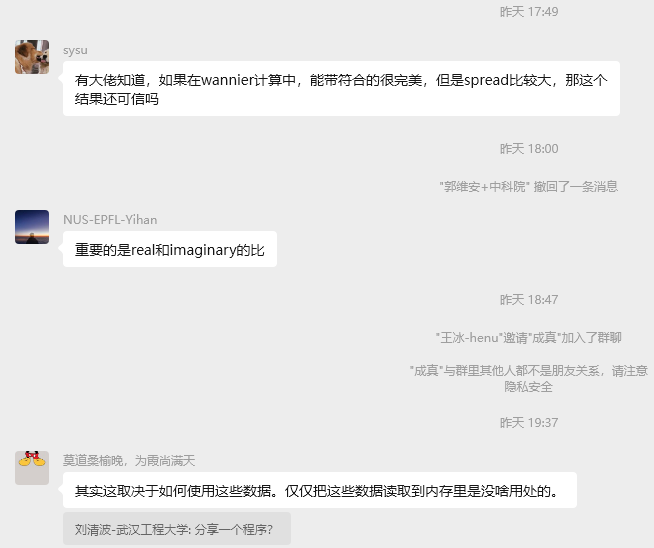
\includegraphics[max width=0.88\linewidth,max height=0.62\textheight,keepaspectratio]{assets/figure-ac3dca427c18.png}
\end{figure}\par\par


\par\begin{figure}[H]\centering

\includegraphics[max width=0.88\linewidth,max height=0.62\textheight,keepaspectratio]{assets/figure-2b384f217479.png}
\end{figure}\par\par


\par\begin{figure}[H]\centering
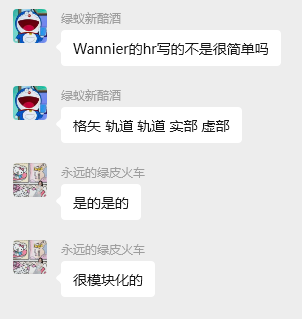
\includegraphics[max width=0.88\linewidth,max height=0.62\textheight,keepaspectratio]{assets/figure-049bd987e9e3.png}
\end{figure}\par\par



\section{利用代码构造紧束缚模型的前置知识}
\begin{articlemeta}
\textbf{日期：}2025-12-06\hfill\textbf{在线原文：}\href{https://marx2001.github.io/sci-note\_posts/20251206-w}{marx2001.github.io}
\end{articlemeta}

\subsubsection{心得笔记}


\subsubsection{对称性约束的六能带紧束缚模型}


用于描述过渡金属二硫化物(TMD)等二维材料的能带结构,特别是在时间反演对称性破缺时,能带出现的谷极化效应(valley polarization)和谷自由度。\par


六能带紧束缚模型是对TMD类材料能带结构的一种简化建模方式,其特点是:\par


\begin{enumerate}
\item 基于轨道选择\par
\item 正负K点能带差异: 在时间反演对称性被破坏时(例如在外磁场或磁性衬底作用下),能带在K和K’点发生能量劈裂和自发谷极化,形成新的自由度——谷自由度(valley degree of freedom),这是实现“谷电子学”的核心基础。\par
\item 群对称性约束: 模型采用具有D3h点群对称性的晶体结构,这是大多数TMD材料(如MoS2、WS2)本征对称性。这个群对称性限制了哈密顿量中各个项的形式,使模型具有物理合理性。\par
\item 哈密顿量表达: 在考虑对称性(如镜面对称、旋转对称等)和晶格结构的基础上,六能带模型构建一个包含6个基态波函数的哈密顿量,用于计算电子的能带结构。\par
\end{enumerate}


Q1:是否有其他数目能带的紧束缚模型?针对每种不同的材料,各种材料对应的紧束缚模型不同吗?\par


A1: 
\par\begin{figure}[H]\centering
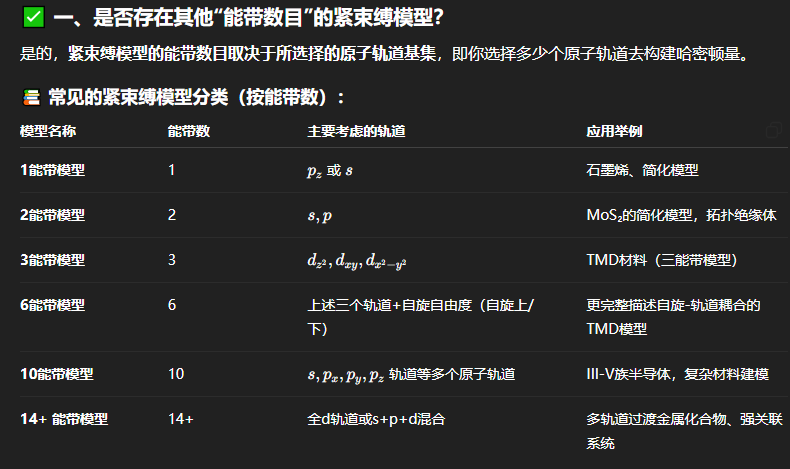
\includegraphics[max width=0.88\linewidth,max height=0.62\textheight,keepaspectratio]{assets/figure-ca38876f2a49.png}
\end{figure}\par
 
\par\begin{figure}[H]\centering
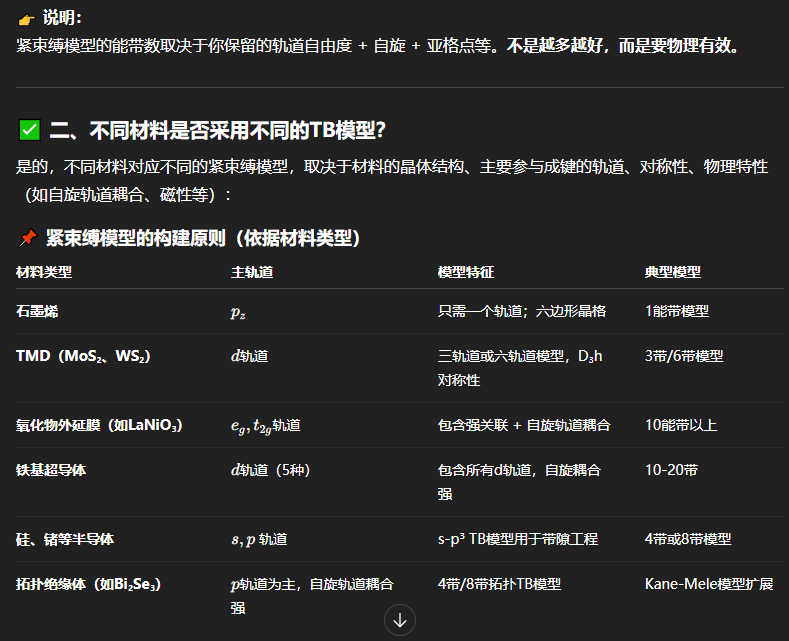
\includegraphics[max width=0.88\linewidth,max height=0.62\textheight,keepaspectratio]{assets/figure-e28763563161.png}
\end{figure}\par\par


\chapter{阶段心得与研究总结}
\begin{partbox}本专题收录 4 篇文章。\end{partbox}

\section{心得笔记1}
\begin{articlemeta}
\textbf{日期：}2025-10-22\hfill\textbf{在线原文：}\href{https://marx2001.github.io/sci-note\_posts/20251022-h}{marx2001.github.io}
\end{articlemeta}

\subsubsection{1}


杂质能级的判断——flat band的出现。杂质原子引入的新能级通常会出现在费米能级附近,表现为局部态(localized states),其在能带结构中表现为非色散性平带(flat bands)在掺杂Pt后,PDOS中出现了新的电 子态,这些态主要由Pt-d轨道与周围Mo-d和S-p轨道混合形成。杂质态通常表现为非常平坦的能带,说明其在实空间中局限在掺杂原子附近。\par


这些态形成于费米能级附近,并不随着动量改变(flat band),意味着它们是局域态,即杂质能级。\par


电荷密度分布,这些能级主要分布在掺杂Pt原子附近及其第一配位壳层内。 进一步确认了这些能级具有局域性,并且源于掺杂引起的对称性破缺\par


掺杂Pt会导致局部晶格结构重构,从而破坏原有的对称性。 这在电子结构上表现为能级分裂和杂质能级的出现。\par


\subsubsection{2}


判断空间群: conda activate mrx\_\allowbreak{}phonopy 然后 phonopy –symmetry –tolerance 0.005\par


\subsubsection{3}


抗磁性桥接原子导致强铁磁耦合的根本原因是:\par


轨道协同:其空轨道或满轨道能与磁性轨道形成对称性匹配的跃迁路径。\par



\section{心得笔记2}
\begin{articlemeta}
\textbf{日期：}2025-11-15\hfill\textbf{在线原文：}\href{https://marx2001.github.io/sci-note\_posts/20251115-h}{marx2001.github.io}
\end{articlemeta}

\subsubsection{1}


利用Lambda固定磁矩使得磁态收敛,四态法计算DMI,首先单点能计算,观察是否顺利收敛,如果不收敛,可以尝试续算,读取上一次的wavecar和chargecar,易于收敛。\par


如果磁矩实在固定不住,需要采用lambda、RWIGS以及M\_\allowbreak{}CONSTR以及I\_\allowbreak{}CONSTRAINED\_\allowbreak{}M的组合进行固定磁矩操作,Lambda的值必须要经过测试,因为不同lambda的值对于收敛后的磁矩 影响极大,需要让Lamdba促进收敛的同时,将磁矩拉到和静态自洽计算即lamdba=0的时候的磁矩大小一致,所以lambda取不同的数值进行磁矩测试是十分必要的。\par


lambda的大小不同,会让磁矩接近静态自洽计算的磁矩,需要让加入lambda后的能量与静态自洽的能量相减,如果加入lambda后的体系能量更低,且磁矩合适,那么这个lambda值就是合理的。\par


\subsubsection{2}


a方向滑移0.5个晶格常数的材料的J的AFM2不收敛,尝试固定磁矩的一套tag不管用+Algo默认,后改用ALGO=ALL+读取上一步的CHGCAR和WAVECAR进行计算,成功收敛,哦对,还需要添加SAXIS=0 0 1\par



\section{EuIn2As2高阶拓扑绝缘体笔记}
\begin{articlemeta}
\textbf{日期：}2025-12-29\hfill\textbf{在线原文：}\href{https://marx2001.github.io/sci-note\_posts/20251229-xinde}{marx2001.github.io}
\end{articlemeta}

\subsubsection{心得笔记}


\par\begin{figure}[H]\centering
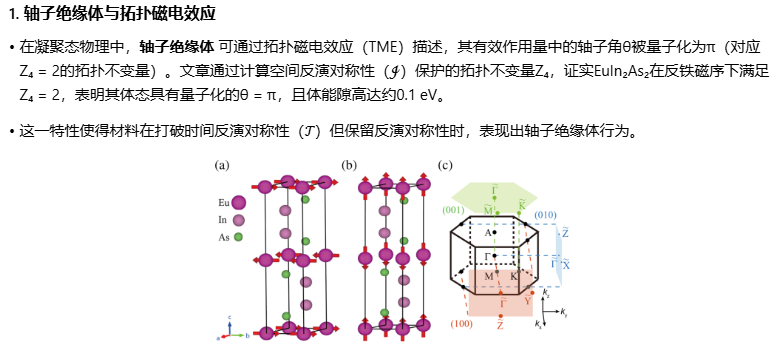
\includegraphics[max width=0.88\linewidth,max height=0.62\textheight,keepaspectratio]{assets/figure-aaf3a42bf79c.png}
\end{figure}\par
 
\par\begin{figure}[H]\centering
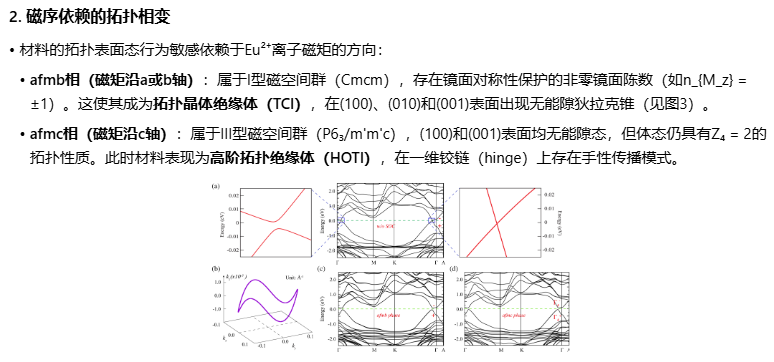
\includegraphics[max width=0.88\linewidth,max height=0.62\textheight,keepaspectratio]{assets/figure-e22453941771.png}
\end{figure}\par
 
\par\begin{figure}[H]\centering
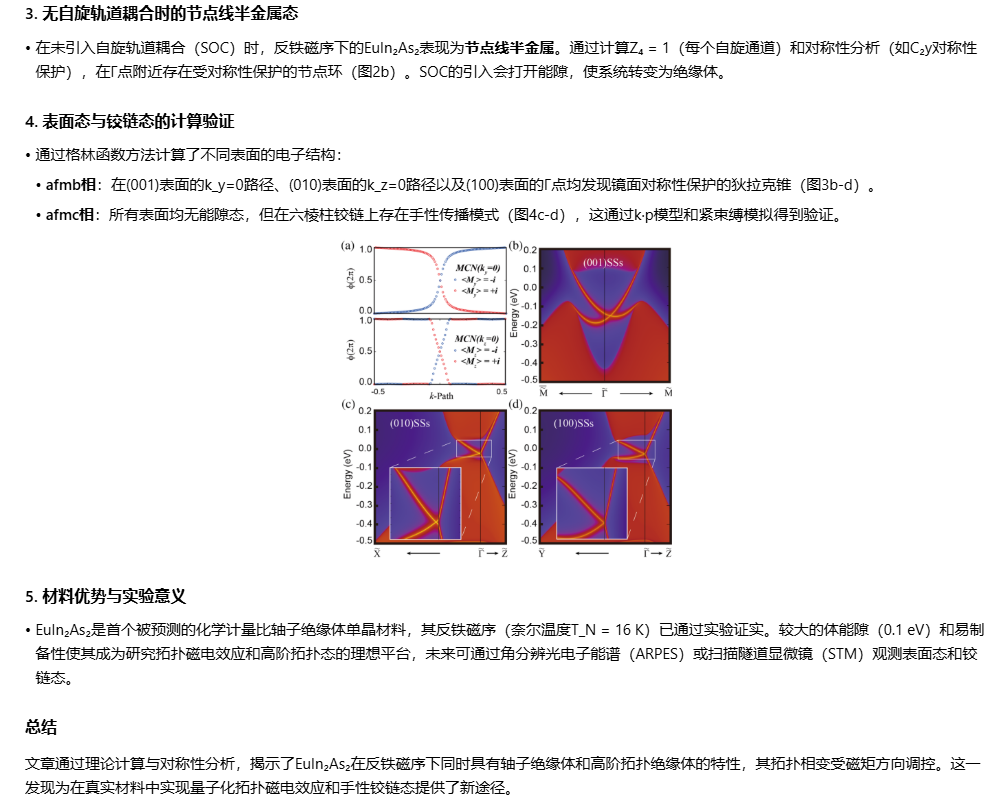
\includegraphics[max width=0.88\linewidth,max height=0.62\textheight,keepaspectratio]{assets/figure-c03c7c7154df.png}
\end{figure}\par
 
\par\begin{figure}[H]\centering
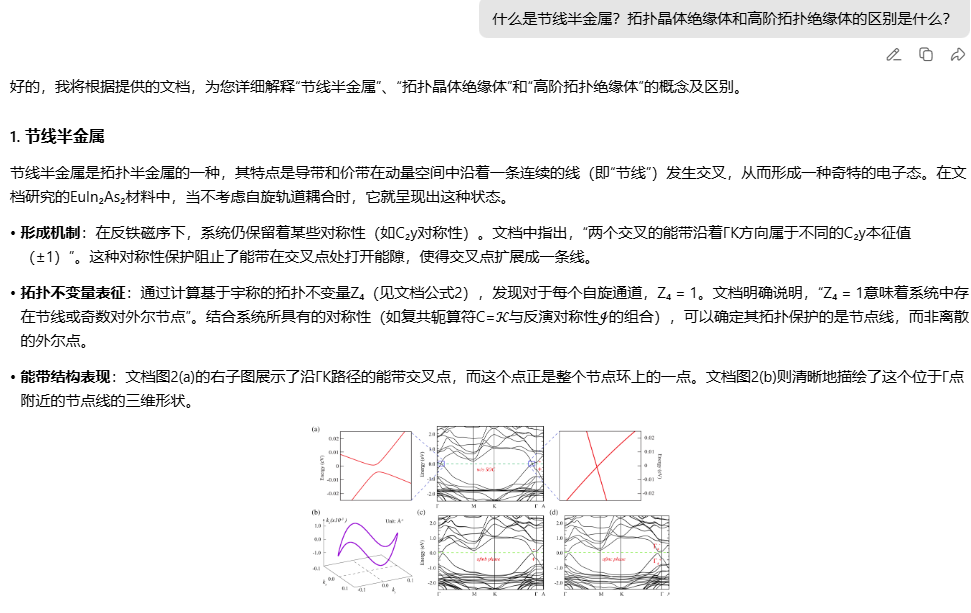
\includegraphics[max width=0.88\linewidth,max height=0.62\textheight,keepaspectratio]{assets/figure-5a530c20f5df.png}
\end{figure}\par
 
\par\begin{figure}[H]\centering
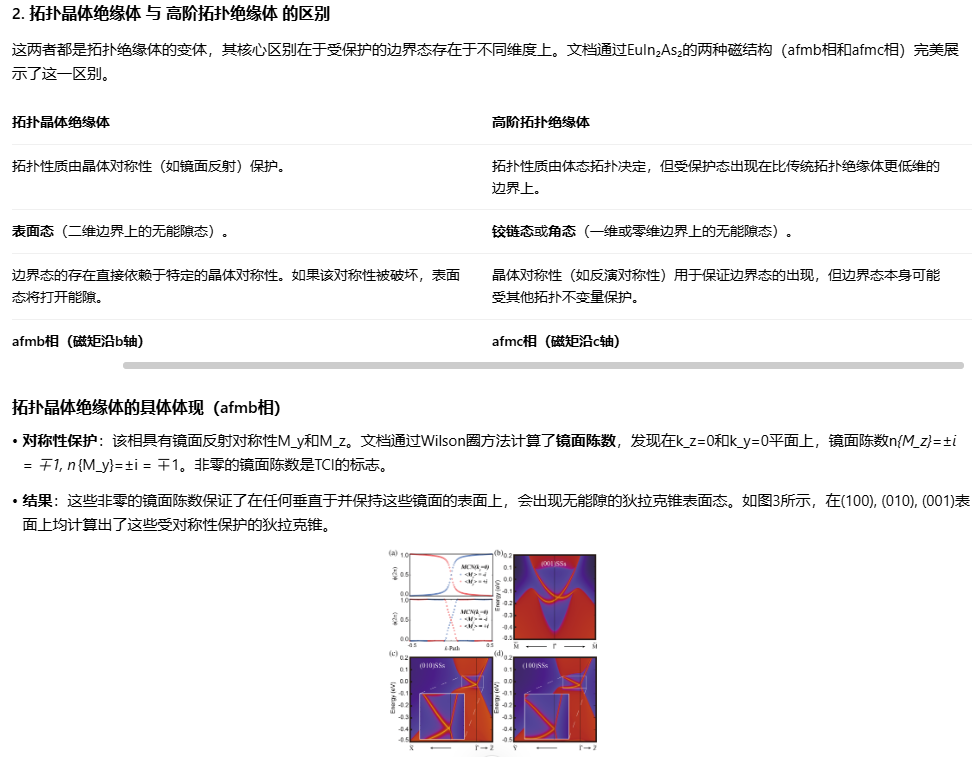
\includegraphics[max width=0.88\linewidth,max height=0.62\textheight,keepaspectratio]{assets/figure-31fb2f8b3003.png}
\end{figure}\par
 
\par\begin{figure}[H]\centering
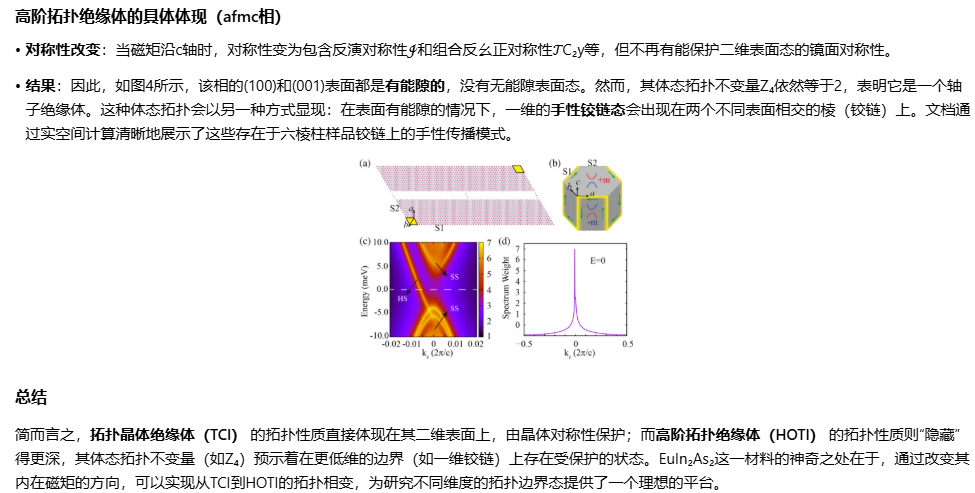
\includegraphics[max width=0.88\linewidth,max height=0.62\textheight,keepaspectratio]{assets/figure-f6ea65d48347.png}
\end{figure}\par
 
\par\begin{figure}[H]\centering
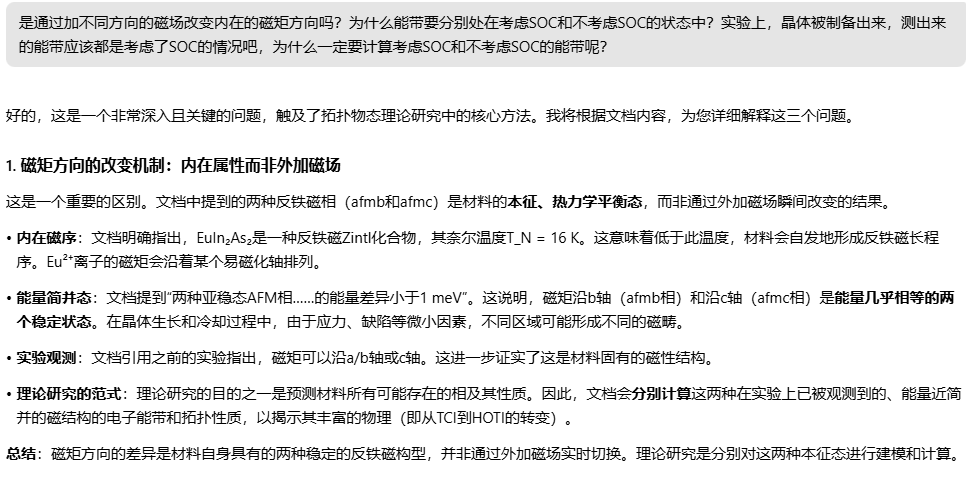
\includegraphics[max width=0.88\linewidth,max height=0.62\textheight,keepaspectratio]{assets/figure-a583c4f09bc6.png}
\end{figure}\par
 
\par\begin{figure}[H]\centering
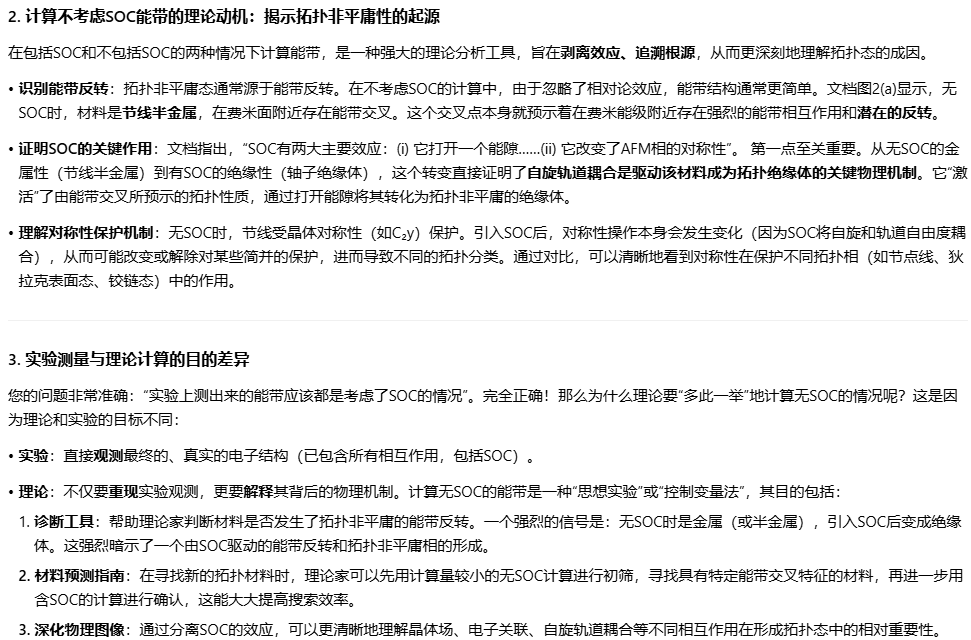
\includegraphics[max width=0.88\linewidth,max height=0.62\textheight,keepaspectratio]{assets/figure-f798f8a1fb4b.png}
\end{figure}\par
 
\par\begin{figure}[H]\centering

\includegraphics[max width=0.88\linewidth,max height=0.62\textheight,keepaspectratio]{assets/figure-6091cc9668a5.png}
\end{figure}\par
 
\par\begin{figure}[H]\centering
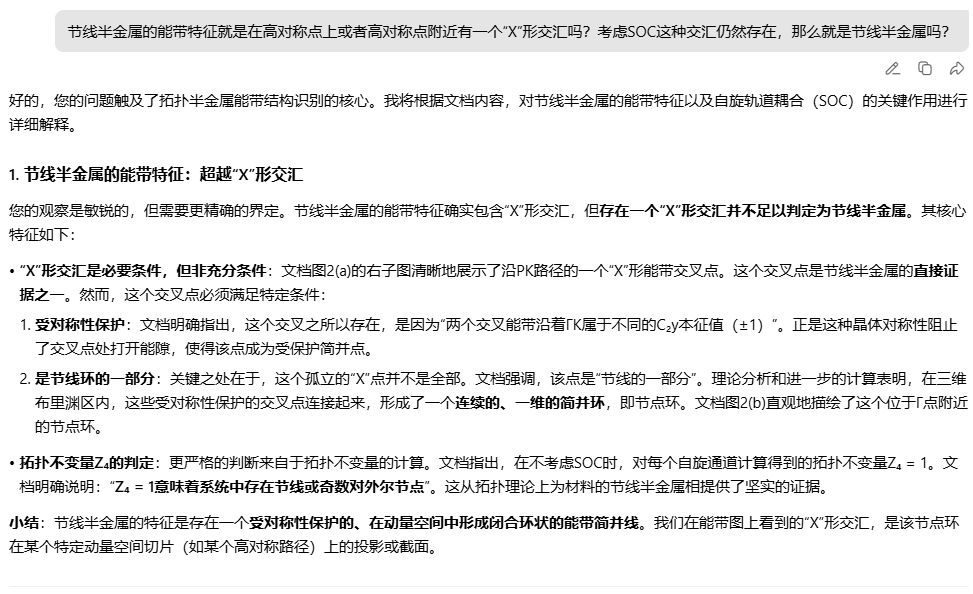
\includegraphics[max width=0.88\linewidth,max height=0.62\textheight,keepaspectratio]{assets/figure-33bda8d3a6ff.png}
\end{figure}\par
 
\par\begin{figure}[H]\centering
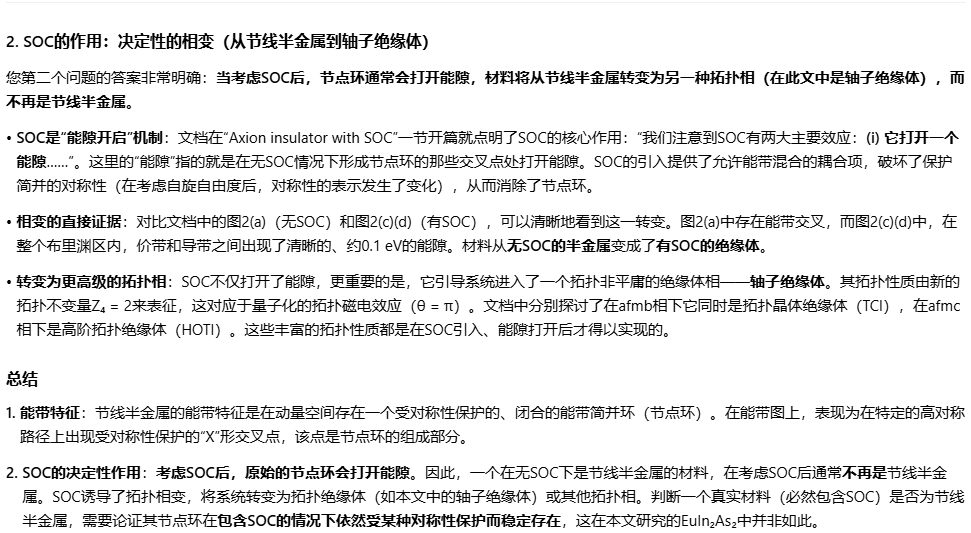
\includegraphics[max width=0.88\linewidth,max height=0.62\textheight,keepaspectratio]{assets/figure-a5d7bec8faff.png}
\end{figure}\par
 
\par\begin{figure}[H]\centering
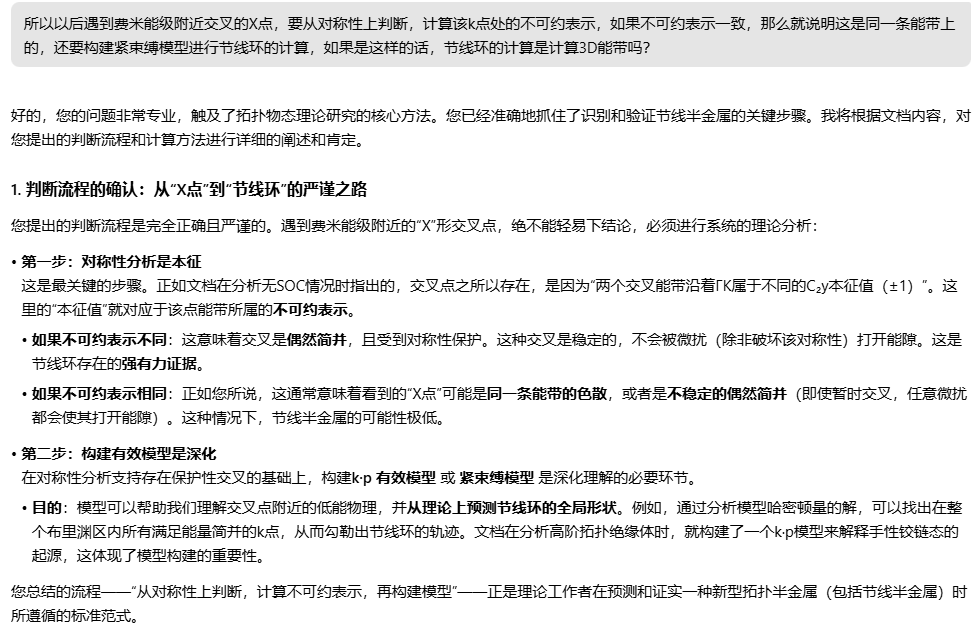
\includegraphics[max width=0.88\linewidth,max height=0.62\textheight,keepaspectratio]{assets/figure-2a01a31f4c7a.png}
\end{figure}\par
 
\par\begin{figure}[H]\centering
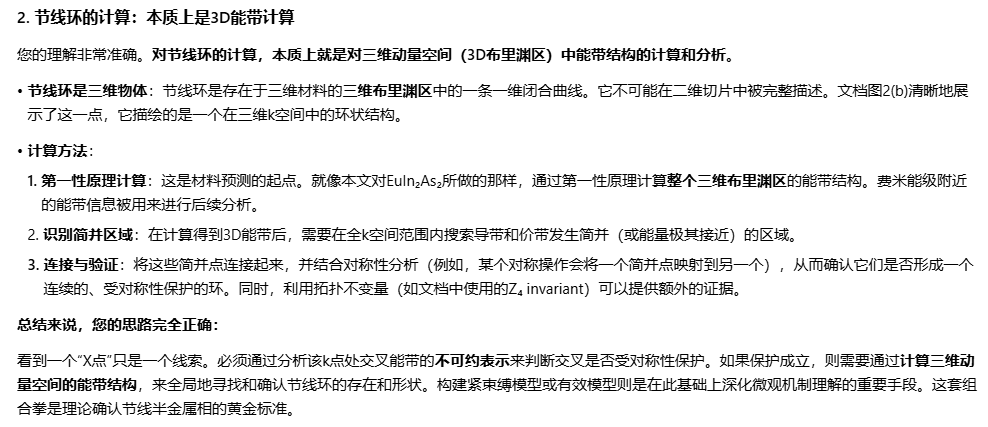
\includegraphics[max width=0.88\linewidth,max height=0.62\textheight,keepaspectratio]{assets/figure-56668064cbe7.png}
\end{figure}\par\par



\section{EuIn2As2高阶拓扑绝缘体笔记2}
\begin{articlemeta}
\textbf{日期：}2025-12-29\hfill\textbf{在线原文：}\href{https://marx2001.github.io/sci-note\_posts/20251230456}{marx2001.github.io}
\end{articlemeta}

\subsubsection{心得笔记}


\par\begin{figure}[H]\centering
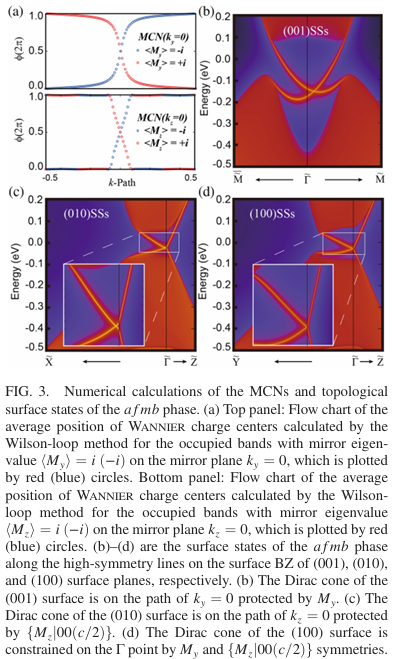
\includegraphics[max width=0.88\linewidth,max height=0.62\textheight,keepaspectratio]{assets/figure-2f5b2428140b.png}
\end{figure}\par
 
\par\begin{figure}[H]\centering
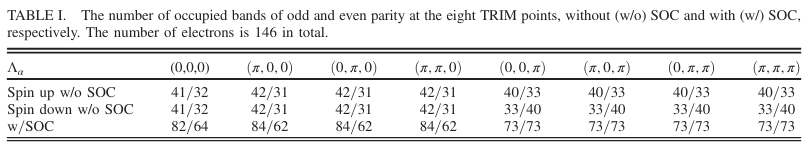
\includegraphics[max width=0.88\linewidth,max height=0.62\textheight,keepaspectratio]{assets/figure-34f2c6ba20fd.png}
\end{figure}\par
 
\par\begin{figure}[H]\centering
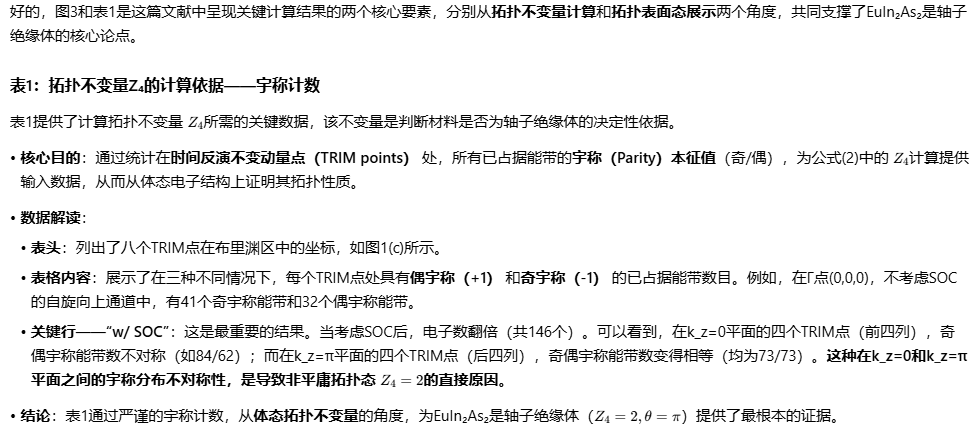
\includegraphics[max width=0.88\linewidth,max height=0.62\textheight,keepaspectratio]{assets/figure-422d2acae09d.png}
\end{figure}\par
 
\par\begin{figure}[H]\centering
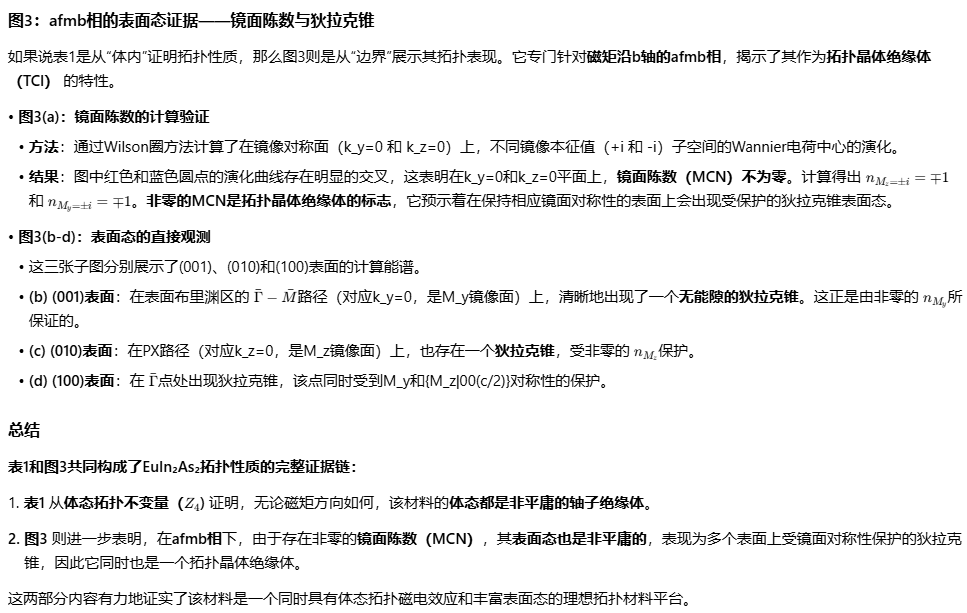
\includegraphics[max width=0.88\linewidth,max height=0.62\textheight,keepaspectratio]{assets/figure-ac28b8f42371.png}
\end{figure}\par
 
\par\begin{figure}[H]\centering
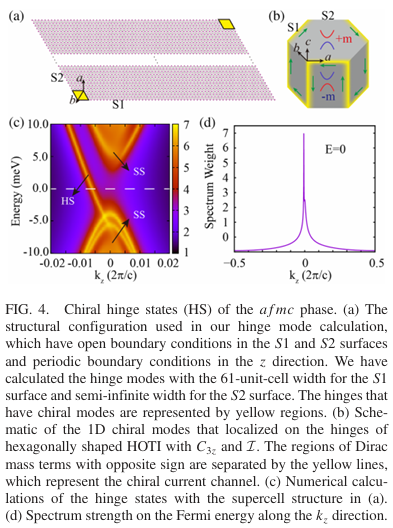
\includegraphics[max width=0.88\linewidth,max height=0.62\textheight,keepaspectratio]{assets/figure-f1cb3f01749d.png}
\end{figure}\par
 
\par\begin{figure}[H]\centering
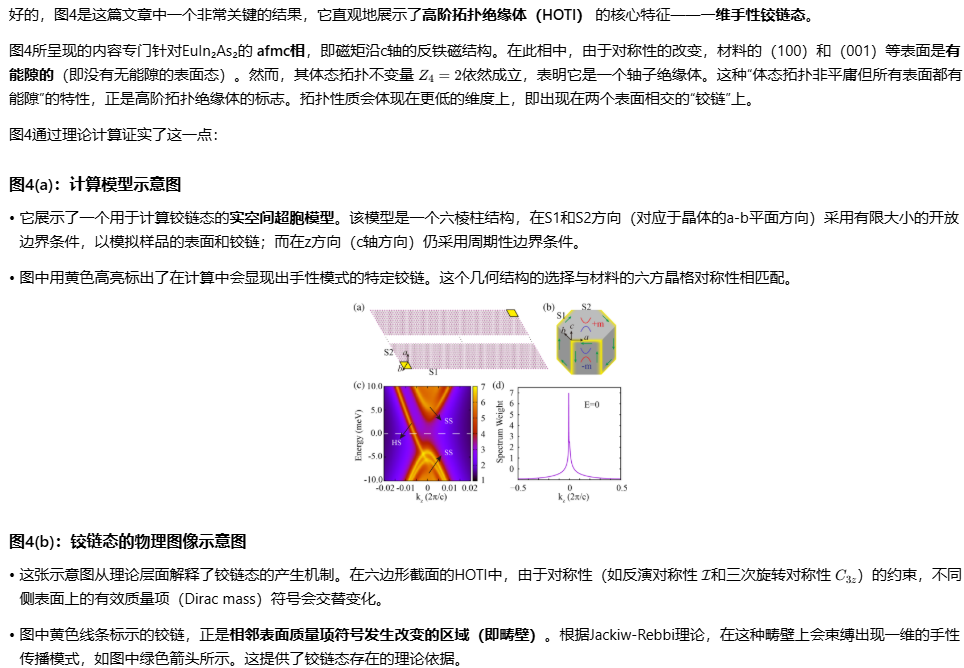
\includegraphics[max width=0.88\linewidth,max height=0.62\textheight,keepaspectratio]{assets/figure-6011523f1d6b.png}
\end{figure}\par
 
\par\begin{figure}[H]\centering
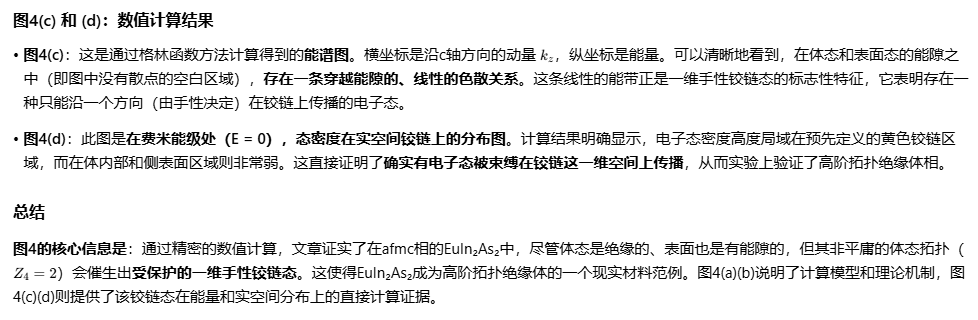
\includegraphics[max width=0.88\linewidth,max height=0.62\textheight,keepaspectratio]{assets/figure-ab551cbdb8f2.png}
\end{figure}\par
 
\par\begin{figure}[H]\centering
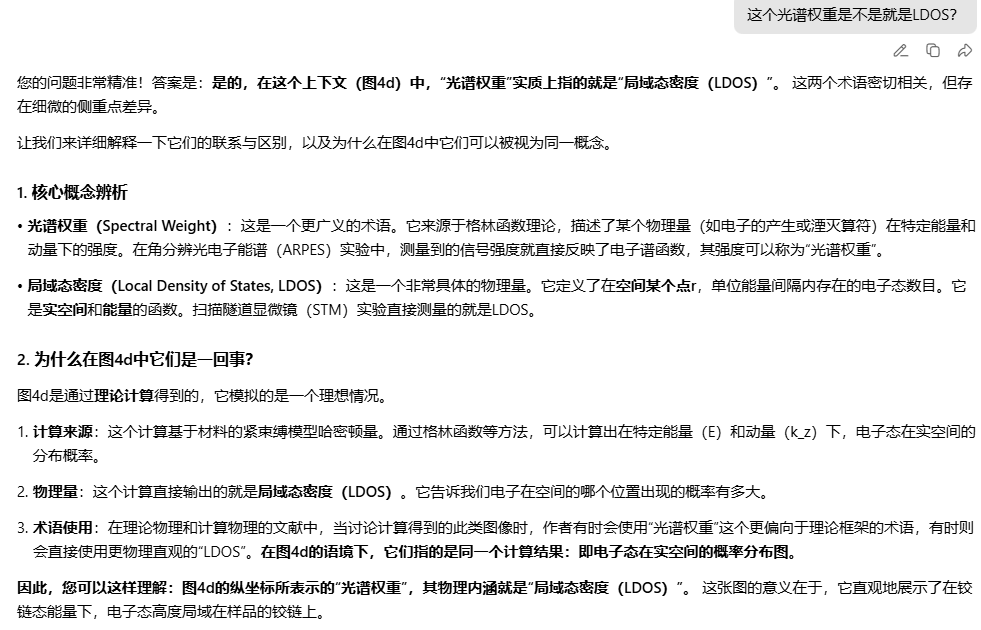
\includegraphics[max width=0.88\linewidth,max height=0.62\textheight,keepaspectratio]{assets/figure-08d3e1cf98c7.png}
\end{figure}\par
 
\par\begin{figure}[H]\centering
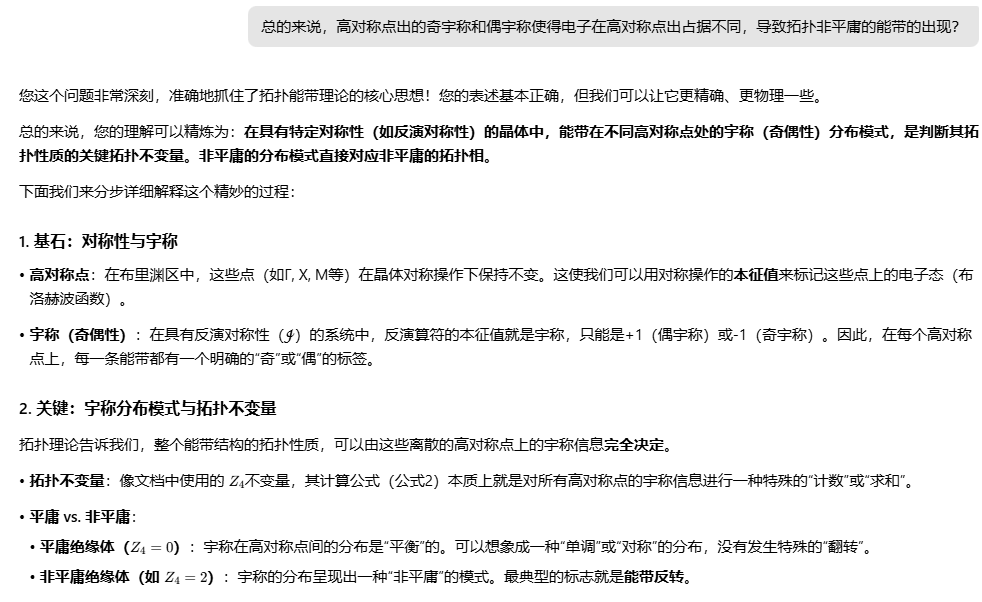
\includegraphics[max width=0.88\linewidth,max height=0.62\textheight,keepaspectratio]{assets/figure-857a8cdba63e.png}
\end{figure}\par
 
\par\begin{figure}[H]\centering
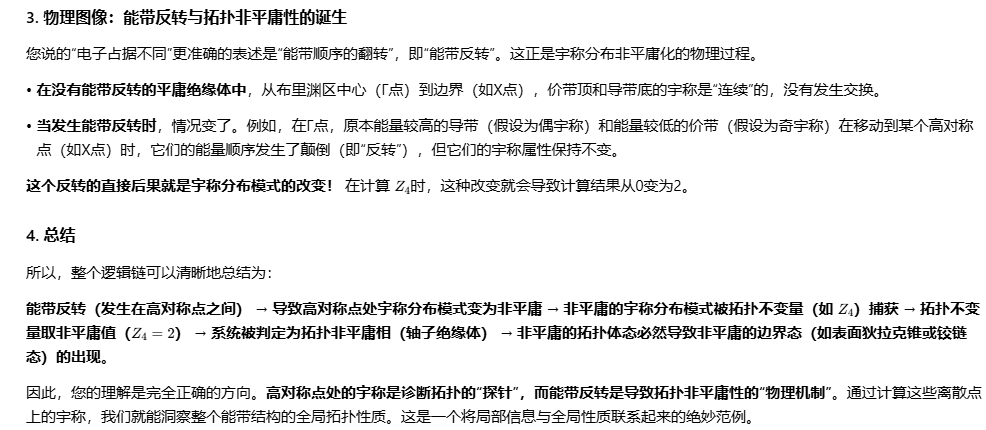
\includegraphics[max width=0.88\linewidth,max height=0.62\textheight,keepaspectratio]{assets/figure-422c2f3392b3.png}
\end{figure}\par
 
\par\begin{figure}[H]\centering
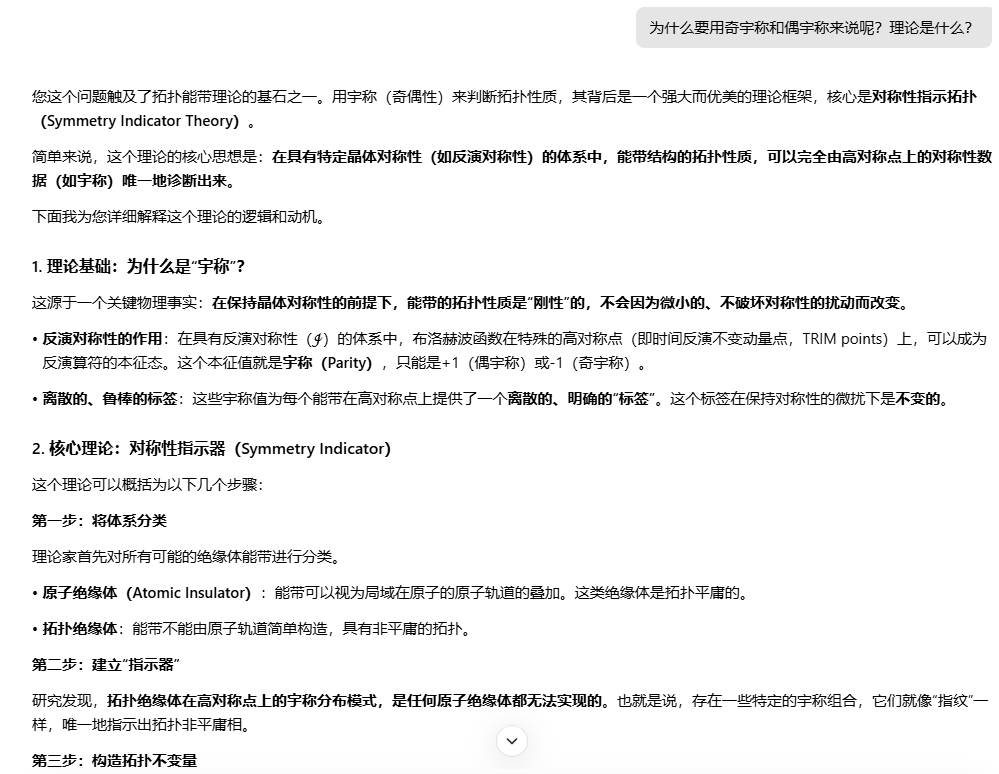
\includegraphics[max width=0.88\linewidth,max height=0.62\textheight,keepaspectratio]{assets/figure-ebf45411ad37.png}
\end{figure}\par
 
\par\begin{figure}[H]\centering
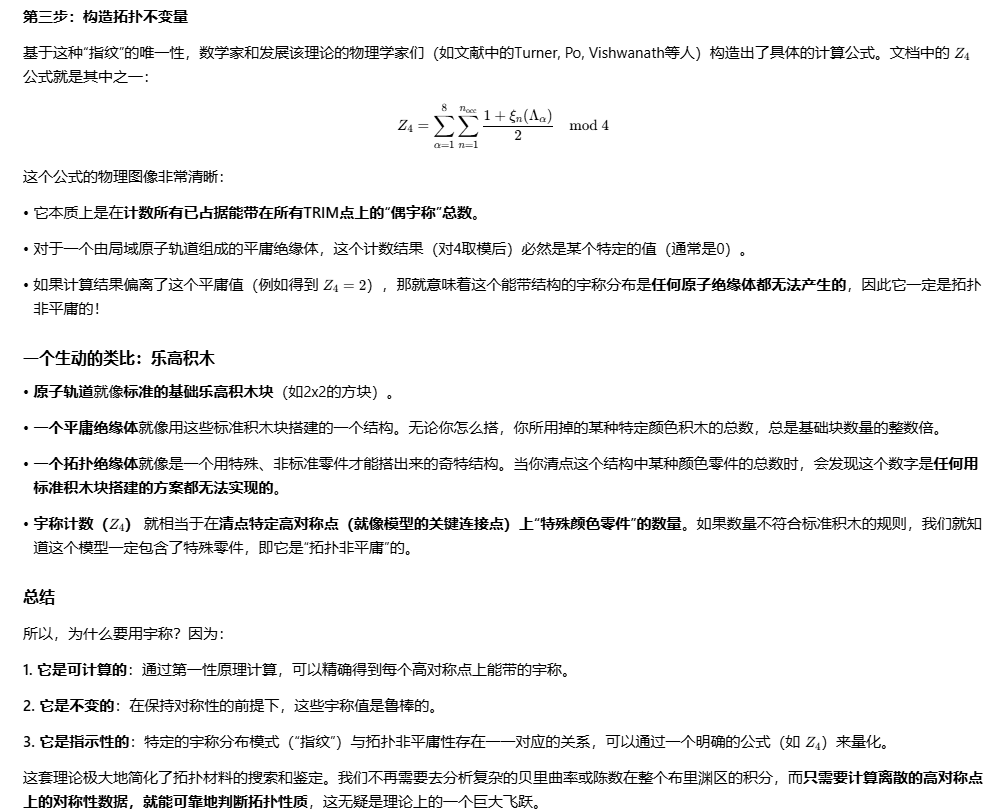
\includegraphics[max width=0.88\linewidth,max height=0.62\textheight,keepaspectratio]{assets/figure-75c998601252.png}
\end{figure}\par
 
\par\begin{figure}[H]\centering
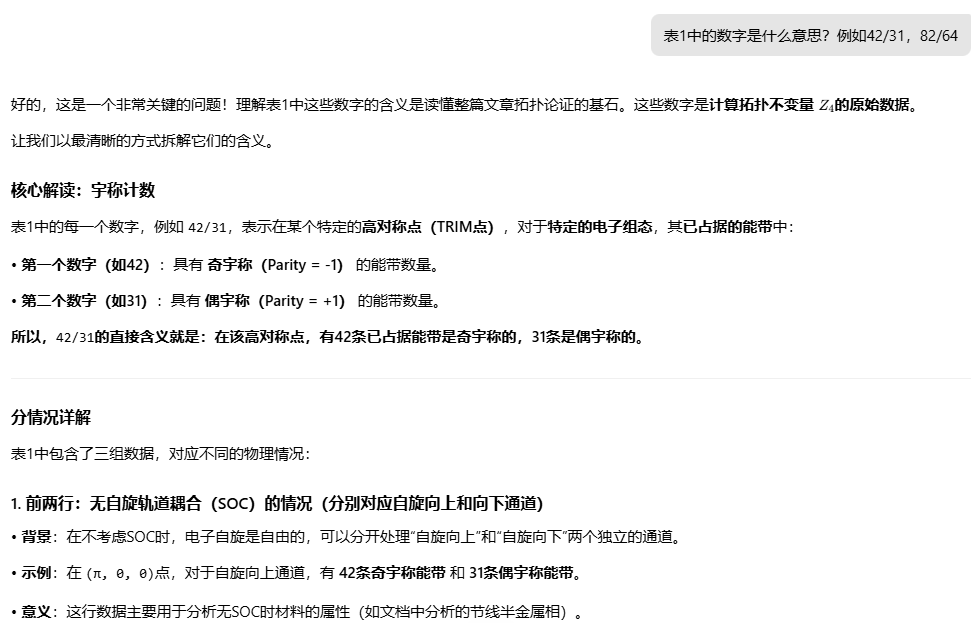
\includegraphics[max width=0.88\linewidth,max height=0.62\textheight,keepaspectratio]{assets/figure-8ee02f59513c.png}
\end{figure}\par
 
\par\begin{figure}[H]\centering
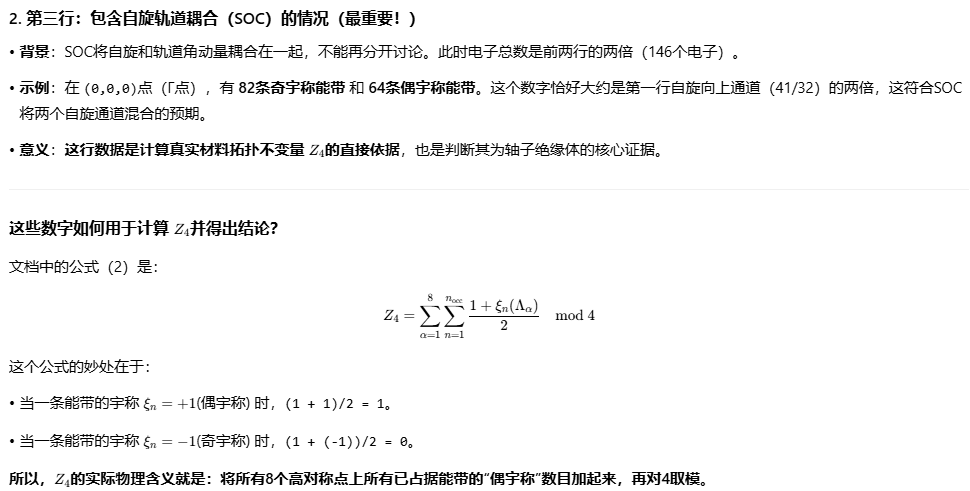
\includegraphics[max width=0.88\linewidth,max height=0.62\textheight,keepaspectratio]{assets/figure-f2d52503788c.png}
\end{figure}\par
 
\par\begin{figure}[H]\centering
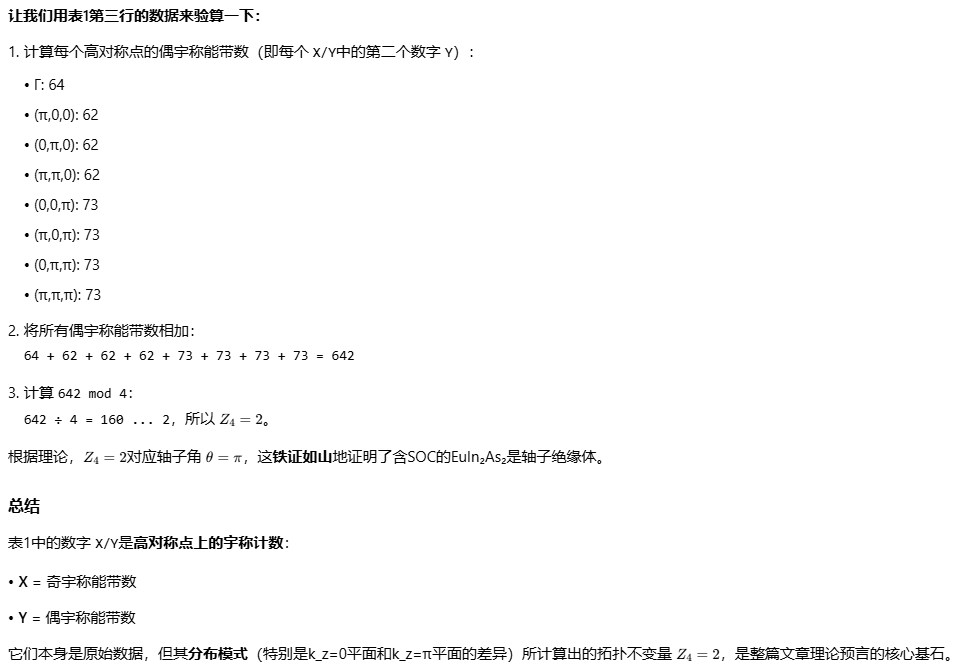
\includegraphics[max width=0.88\linewidth,max height=0.62\textheight,keepaspectratio]{assets/figure-feaab35e2980.png}
\end{figure}\par\par


\appendix
\chapter{完整代码清单}
本附录按正文文章号排序，仅收录不适合在正文展开的较长代码。简短命令与短代码已在正文代码框中直接展示；全部代码块仍保存于工程 \texttt{code/} 目录，便于复制、检索与复现。
\section*{vasp计算态密度}
\phantomsection\label{code:1:1}
\subsection*{代码清单 A.1.1（python，38 行）}
\VerbatimInput[fontsize=\scriptsize,breaklines=true,breakanywhere=true,tabsize=2]{code/001-001.py}
\medskip
\section*{vasp计算投影能带}
\phantomsection\label{code:2:1}
\subsection*{代码清单 A.2.1（python，19 行）}
\VerbatimInput[fontsize=\scriptsize,breaklines=true,breakanywhere=true,tabsize=2]{code/002-001.py}
\medskip
\phantomsection\label{code:2:2}
\subsection*{代码清单 A.2.2（python，658 行）}
\VerbatimInput[fontsize=\scriptsize,breaklines=true,breakanywhere=true,tabsize=2]{code/002-002.py}
\medskip
\phantomsection\label{code:2:3}
\subsection*{代码清单 A.2.3（python，70 行）}
\VerbatimInput[fontsize=\scriptsize,breaklines=true,breakanywhere=true,tabsize=2]{code/002-003.py}
\medskip
\phantomsection\label{code:2:4}
\subsection*{代码清单 A.2.4（python，651 行）}
\VerbatimInput[fontsize=\scriptsize,breaklines=true,breakanywhere=true,tabsize=2]{code/002-004.py}
\medskip
\section*{vasp计算能带}
\phantomsection\label{code:3:1}
\subsection*{代码清单 A.3.1（python，36 行）}
\VerbatimInput[fontsize=\scriptsize,breaklines=true,breakanywhere=true,tabsize=2]{code/003-001.py}
\medskip
\phantomsection\label{code:3:2}
\subsection*{代码清单 A.3.2（python，37 行）}
\VerbatimInput[fontsize=\scriptsize,breaklines=true,breakanywhere=true,tabsize=2]{code/003-002.py}
\medskip
\section*{vasp计算磁耦合参数大小}
\phantomsection\label{code:4:1}
\subsection*{代码清单 A.4.1（shell，40 行）}
\VerbatimInput[fontsize=\scriptsize,breaklines=true,breakanywhere=true,tabsize=2]{code/004-001.sh}
\medskip
\phantomsection\label{code:4:2}
\subsection*{代码清单 A.4.2（shell，40 行）}
\VerbatimInput[fontsize=\scriptsize,breaklines=true,breakanywhere=true,tabsize=2]{code/004-002.sh}
\medskip
\phantomsection\label{code:4:3}
\subsection*{代码清单 A.4.3（shell，40 行）}
\VerbatimInput[fontsize=\scriptsize,breaklines=true,breakanywhere=true,tabsize=2]{code/004-003.sh}
\medskip
\phantomsection\label{code:4:4}
\subsection*{代码清单 A.4.4（shell，40 行）}
\VerbatimInput[fontsize=\scriptsize,breaklines=true,breakanywhere=true,tabsize=2]{code/004-004.sh}
\medskip
\phantomsection\label{code:4:5}
\subsection*{代码清单 A.4.5（shell，41 行）}
\VerbatimInput[fontsize=\scriptsize,breaklines=true,breakanywhere=true,tabsize=2]{code/004-005.sh}
\medskip
\phantomsection\label{code:4:6}
\subsection*{代码清单 A.4.6（shell，46 行）}
\VerbatimInput[fontsize=\scriptsize,breaklines=true,breakanywhere=true,tabsize=2]{code/004-006.sh}
\medskip
\phantomsection\label{code:4:7}
\subsection*{代码清单 A.4.7（shell，41 行）}
\VerbatimInput[fontsize=\scriptsize,breaklines=true,breakanywhere=true,tabsize=2]{code/004-007.sh}
\medskip
\phantomsection\label{code:4:8}
\subsection*{代码清单 A.4.8（shell，41 行）}
\VerbatimInput[fontsize=\scriptsize,breaklines=true,breakanywhere=true,tabsize=2]{code/004-008.sh}
\medskip
\phantomsection\label{code:4:9}
\subsection*{代码清单 A.4.9（shell，41 行）}
\VerbatimInput[fontsize=\scriptsize,breaklines=true,breakanywhere=true,tabsize=2]{code/004-009.sh}
\medskip
\phantomsection\label{code:4:10}
\subsection*{代码清单 A.4.10（shell，51 行）}
\VerbatimInput[fontsize=\scriptsize,breaklines=true,breakanywhere=true,tabsize=2]{code/004-010.sh}
\medskip
\section*{vasp计算DMI大小}
\phantomsection\label{code:5:1}
\subsection*{代码清单 A.5.1（python，39 行）}
\VerbatimInput[fontsize=\scriptsize,breaklines=true,breakanywhere=true,tabsize=2]{code/005-001.py}
\medskip
\phantomsection\label{code:5:2}
\subsection*{代码清单 A.5.2（shell，39 行）}
\VerbatimInput[fontsize=\scriptsize,breaklines=true,breakanywhere=true,tabsize=2]{code/005-002.sh}
\medskip
\phantomsection\label{code:5:3}
\subsection*{代码清单 A.5.3（shell，46 行）}
\VerbatimInput[fontsize=\scriptsize,breaklines=true,breakanywhere=true,tabsize=2]{code/005-003.sh}
\medskip
\section*{(文献整理)块体材料 DMI 的第一性原理提取方法}
\phantomsection\label{code:6:1}
\subsection*{代码清单 A.6.1（shell，5 行）}
\VerbatimInput[fontsize=\scriptsize,breaklines=true,breakanywhere=true,tabsize=2]{code/006-001.sh}
\medskip
\phantomsection\label{code:6:2}
\subsection*{代码清单 A.6.2（text，4 行）}
\VerbatimInput[fontsize=\scriptsize,breaklines=true,breakanywhere=true,tabsize=2]{code/006-002.txt}
\medskip
\phantomsection\label{code:6:3}
\subsection*{代码清单 A.6.3（shell，5 行）}
\VerbatimInput[fontsize=\scriptsize,breaklines=true,breakanywhere=true,tabsize=2]{code/006-003.sh}
\medskip
\phantomsection\label{code:6:4}
\subsection*{代码清单 A.6.4（shell，1 行）}
\VerbatimInput[fontsize=\scriptsize,breaklines=true,breakanywhere=true,tabsize=2]{code/006-004.sh}
\medskip
\phantomsection\label{code:6:5}
\subsection*{代码清单 A.6.5（text，4 行）}
\VerbatimInput[fontsize=\scriptsize,breaklines=true,breakanywhere=true,tabsize=2]{code/006-005.txt}
\medskip
\phantomsection\label{code:6:6}
\subsection*{代码清单 A.6.6（shell，3 行）}
\VerbatimInput[fontsize=\scriptsize,breaklines=true,breakanywhere=true,tabsize=2]{code/006-006.sh}
\medskip
\phantomsection\label{code:6:7}
\subsection*{代码清单 A.6.7（text，5 行）}
\VerbatimInput[fontsize=\scriptsize,breaklines=true,breakanywhere=true,tabsize=2]{code/006-007.txt}
\medskip
\phantomsection\label{code:6:8}
\subsection*{代码清单 A.6.8（text，4 行）}
\VerbatimInput[fontsize=\scriptsize,breaklines=true,breakanywhere=true,tabsize=2]{code/006-008.txt}
\medskip
\phantomsection\label{code:6:9}
\subsection*{代码清单 A.6.9（shell，4 行）}
\VerbatimInput[fontsize=\scriptsize,breaklines=true,breakanywhere=true,tabsize=2]{code/006-009.sh}
\medskip
\phantomsection\label{code:6:10}
\subsection*{代码清单 A.6.10（shell，1 行）}
\VerbatimInput[fontsize=\scriptsize,breaklines=true,breakanywhere=true,tabsize=2]{code/006-010.sh}
\medskip
\phantomsection\label{code:6:11}
\subsection*{代码清单 A.6.11（text，4 行）}
\VerbatimInput[fontsize=\scriptsize,breaklines=true,breakanywhere=true,tabsize=2]{code/006-011.txt}
\medskip
\phantomsection\label{code:6:12}
\subsection*{代码清单 A.6.12（text，4 行）}
\VerbatimInput[fontsize=\scriptsize,breaklines=true,breakanywhere=true,tabsize=2]{code/006-012.txt}
\medskip
\phantomsection\label{code:6:13}
\subsection*{代码清单 A.6.13（shell，3 行）}
\VerbatimInput[fontsize=\scriptsize,breaklines=true,breakanywhere=true,tabsize=2]{code/006-013.sh}
\medskip
\phantomsection\label{code:6:14}
\subsection*{代码清单 A.6.14（text，5 行）}
\VerbatimInput[fontsize=\scriptsize,breaklines=true,breakanywhere=true,tabsize=2]{code/006-014.txt}
\medskip
\phantomsection\label{code:6:15}
\subsection*{代码清单 A.6.15（shell，3 行）}
\VerbatimInput[fontsize=\scriptsize,breaklines=true,breakanywhere=true,tabsize=2]{code/006-015.sh}
\medskip
\phantomsection\label{code:6:16}
\subsection*{代码清单 A.6.16（text，5 行）}
\VerbatimInput[fontsize=\scriptsize,breaklines=true,breakanywhere=true,tabsize=2]{code/006-016.txt}
\medskip
\phantomsection\label{code:6:17}
\subsection*{代码清单 A.6.17（shell，3 行）}
\VerbatimInput[fontsize=\scriptsize,breaklines=true,breakanywhere=true,tabsize=2]{code/006-017.sh}
\medskip
\phantomsection\label{code:6:18}
\subsection*{代码清单 A.6.18（text，4 行）}
\VerbatimInput[fontsize=\scriptsize,breaklines=true,breakanywhere=true,tabsize=2]{code/006-018.txt}
\medskip
\phantomsection\label{code:6:19}
\subsection*{代码清单 A.6.19（shell，1 行）}
\VerbatimInput[fontsize=\scriptsize,breaklines=true,breakanywhere=true,tabsize=2]{code/006-019.sh}
\medskip
\phantomsection\label{code:6:20}
\subsection*{代码清单 A.6.20（text，5 行）}
\VerbatimInput[fontsize=\scriptsize,breaklines=true,breakanywhere=true,tabsize=2]{code/006-020.txt}
\medskip
\phantomsection\label{code:6:21}
\subsection*{代码清单 A.6.21（shell，3 行）}
\VerbatimInput[fontsize=\scriptsize,breaklines=true,breakanywhere=true,tabsize=2]{code/006-021.sh}
\medskip
\phantomsection\label{code:6:22}
\subsection*{代码清单 A.6.22（text，3 行）}
\VerbatimInput[fontsize=\scriptsize,breaklines=true,breakanywhere=true,tabsize=2]{code/006-022.txt}
\medskip
\phantomsection\label{code:6:23}
\subsection*{代码清单 A.6.23（text，1 行）}
\VerbatimInput[fontsize=\scriptsize,breaklines=true,breakanywhere=true,tabsize=2]{code/006-023.txt}
\medskip
\phantomsection\label{code:6:24}
\subsection*{代码清单 A.6.24（text，2 行）}
\VerbatimInput[fontsize=\scriptsize,breaklines=true,breakanywhere=true,tabsize=2]{code/006-024.txt}
\medskip
\phantomsection\label{code:6:25}
\subsection*{代码清单 A.6.25（text，3 行）}
\VerbatimInput[fontsize=\scriptsize,breaklines=true,breakanywhere=true,tabsize=2]{code/006-025.txt}
\medskip
\phantomsection\label{code:6:26}
\subsection*{代码清单 A.6.26（text，1 行）}
\VerbatimInput[fontsize=\scriptsize,breaklines=true,breakanywhere=true,tabsize=2]{code/006-026.txt}
\medskip
\phantomsection\label{code:6:27}
\subsection*{代码清单 A.6.27（shell，5 行）}
\VerbatimInput[fontsize=\scriptsize,breaklines=true,breakanywhere=true,tabsize=2]{code/006-027.sh}
\medskip
\phantomsection\label{code:6:28}
\subsection*{代码清单 A.6.28（shell，17 行）}
\VerbatimInput[fontsize=\scriptsize,breaklines=true,breakanywhere=true,tabsize=2]{code/006-028.sh}
\medskip
\phantomsection\label{code:6:29}
\subsection*{代码清单 A.6.29（shell，1 行）}
\VerbatimInput[fontsize=\scriptsize,breaklines=true,breakanywhere=true,tabsize=2]{code/006-029.sh}
\medskip
\phantomsection\label{code:6:30}
\subsection*{代码清单 A.6.30（shell，1 行）}
\VerbatimInput[fontsize=\scriptsize,breaklines=true,breakanywhere=true,tabsize=2]{code/006-030.sh}
\medskip
\phantomsection\label{code:6:31}
\subsection*{代码清单 A.6.31（shell，1 行）}
\VerbatimInput[fontsize=\scriptsize,breaklines=true,breakanywhere=true,tabsize=2]{code/006-031.sh}
\medskip
\phantomsection\label{code:6:32}
\subsection*{代码清单 A.6.32（text，54 行）}
\VerbatimInput[fontsize=\scriptsize,breaklines=true,breakanywhere=true,tabsize=2]{code/006-032.txt}
\medskip
\section*{vasp结构优化}
\phantomsection\label{code:7:1}
\subsection*{代码清单 A.7.1（shell，22 行）}
\VerbatimInput[fontsize=\scriptsize,breaklines=true,breakanywhere=true,tabsize=2]{code/007-001.sh}
\medskip
\phantomsection\label{code:7:2}
\subsection*{代码清单 A.7.2（shell，27 行）}
\VerbatimInput[fontsize=\scriptsize,breaklines=true,breakanywhere=true,tabsize=2]{code/007-002.sh}
\medskip
\section*{Wannier90 学习笔记}
\phantomsection\label{code:8:1}
\subsection*{代码清单 A.8.1（shell，3 行）}
\VerbatimInput[fontsize=\scriptsize,breaklines=true,breakanywhere=true,tabsize=2]{code/008-001.sh}
\medskip
\section*{以Bi烯为例的wannier90表面态计算}
\phantomsection\label{code:9:2}
\subsection*{代码清单 A.9.2（shell，30 行）}
\VerbatimInput[fontsize=\scriptsize,breaklines=true,breakanywhere=true,tabsize=2]{code/009-002.sh}
\medskip
\phantomsection\label{code:9:3}
\subsection*{代码清单 A.9.3（shell，15 行）}
\VerbatimInput[fontsize=\scriptsize,breaklines=true,breakanywhere=true,tabsize=2]{code/009-003.sh}
\medskip
\phantomsection\label{code:9:4}
\subsection*{代码清单 A.9.4（shell，10 行）}
\VerbatimInput[fontsize=\scriptsize,breaklines=true,breakanywhere=true,tabsize=2]{code/009-004.sh}
\medskip
\phantomsection\label{code:9:7}
\subsection*{代码清单 A.9.7（shell，63 行）}
\VerbatimInput[fontsize=\scriptsize,breaklines=true,breakanywhere=true,tabsize=2]{code/009-007.sh}
\medskip
\phantomsection\label{code:9:11}
\subsection*{代码清单 A.9.11（shell，63 行）}
\VerbatimInput[fontsize=\scriptsize,breaklines=true,breakanywhere=true,tabsize=2]{code/009-011.sh}
\medskip
\phantomsection\label{code:9:12}
\subsection*{代码清单 A.9.12（shell，57 行）}
\VerbatimInput[fontsize=\scriptsize,breaklines=true,breakanywhere=true,tabsize=2]{code/009-012.sh}
\medskip
\section*{Wannier90的表面态的参数选择标准1\_\allowbreak{}示例文件的参数注释}
\phantomsection\label{code:11:1}
\subsection*{代码清单 A.11.1（shell，63 行）}
\VerbatimInput[fontsize=\scriptsize,breaklines=true,breakanywhere=true,tabsize=2]{code/011-001.sh}
\medskip
\phantomsection\label{code:11:2}
\subsection*{代码清单 A.11.2（shell，10 行）}
\VerbatimInput[fontsize=\scriptsize,breaklines=true,breakanywhere=true,tabsize=2]{code/011-002.sh}
\medskip
\phantomsection\label{code:11:3}
\subsection*{代码清单 A.11.3（shell，4 行）}
\VerbatimInput[fontsize=\scriptsize,breaklines=true,breakanywhere=true,tabsize=2]{code/011-003.sh}
\medskip
\phantomsection\label{code:11:4}
\subsection*{代码清单 A.11.4（shell，5 行）}
\VerbatimInput[fontsize=\scriptsize,breaklines=true,breakanywhere=true,tabsize=2]{code/011-004.sh}
\medskip
\phantomsection\label{code:11:5}
\subsection*{代码清单 A.11.5（shell，4 行）}
\VerbatimInput[fontsize=\scriptsize,breaklines=true,breakanywhere=true,tabsize=2]{code/011-005.sh}
\medskip
\section*{wannier90的能带拟合步骤}
\phantomsection\label{code:20:1}
\subsection*{代码清单 A.20.1（shell，5 行）}
\VerbatimInput[fontsize=\scriptsize,breaklines=true,breakanywhere=true,tabsize=2]{code/020-001.sh}
\medskip
\phantomsection\label{code:20:2}
\subsection*{代码清单 A.20.2（shell，43 行）}
\VerbatimInput[fontsize=\scriptsize,breaklines=true,breakanywhere=true,tabsize=2]{code/020-002.sh}
\medskip
\phantomsection\label{code:20:3}
\subsection*{代码清单 A.20.3（shell，11 行）}
\VerbatimInput[fontsize=\scriptsize,breaklines=true,breakanywhere=true,tabsize=2]{code/020-003.sh}
\medskip
\phantomsection\label{code:20:4}
\subsection*{代码清单 A.20.4（shell，42 行）}
\VerbatimInput[fontsize=\scriptsize,breaklines=true,breakanywhere=true,tabsize=2]{code/020-004.sh}
\medskip
\phantomsection\label{code:20:5}
\subsection*{代码清单 A.20.5（shell，15 行）}
\VerbatimInput[fontsize=\scriptsize,breaklines=true,breakanywhere=true,tabsize=2]{code/020-005.sh}
\medskip
\phantomsection\label{code:20:6}
\subsection*{代码清单 A.20.6（shell，54 行）}
\VerbatimInput[fontsize=\scriptsize,breaklines=true,breakanywhere=true,tabsize=2]{code/020-006.sh}
\medskip
\phantomsection\label{code:20:7}
\subsection*{代码清单 A.20.7（shell，10 行）}
\VerbatimInput[fontsize=\scriptsize,breaklines=true,breakanywhere=true,tabsize=2]{code/020-007.sh}
\medskip
\section*{pyw90的测试用例}
\phantomsection\label{code:21:2}
\subsection*{代码清单 A.21.2（shell，8 行）}
\VerbatimInput[fontsize=\scriptsize,breaklines=true,breakanywhere=true,tabsize=2]{code/021-002.sh}
\medskip
\phantomsection\label{code:21:3}
\subsection*{代码清单 A.21.3（shell，15 行）}
\VerbatimInput[fontsize=\scriptsize,breaklines=true,breakanywhere=true,tabsize=2]{code/021-003.sh}
\medskip
\phantomsection\label{code:21:4}
\subsection*{代码清单 A.21.4（shell，1 行）}
\VerbatimInput[fontsize=\scriptsize,breaklines=true,breakanywhere=true,tabsize=2]{code/021-004.sh}
\medskip
\phantomsection\label{code:21:5}
\subsection*{代码清单 A.21.5（shell，23 行）}
\VerbatimInput[fontsize=\scriptsize,breaklines=true,breakanywhere=true,tabsize=2]{code/021-005.sh}
\medskip
\phantomsection\label{code:21:6}
\subsection*{代码清单 A.21.6（shell，1 行）}
\VerbatimInput[fontsize=\scriptsize,breaklines=true,breakanywhere=true,tabsize=2]{code/021-006.sh}
\medskip
\phantomsection\label{code:21:7}
\subsection*{代码清单 A.21.7（shell，24 行）}
\VerbatimInput[fontsize=\scriptsize,breaklines=true,breakanywhere=true,tabsize=2]{code/021-007.sh}
\medskip
\phantomsection\label{code:21:8}
\subsection*{代码清单 A.21.8（shell，2 行）}
\VerbatimInput[fontsize=\scriptsize,breaklines=true,breakanywhere=true,tabsize=2]{code/021-008.sh}
\medskip
\phantomsection\label{code:21:9}
\subsection*{代码清单 A.21.9（shell，78 行）}
\VerbatimInput[fontsize=\scriptsize,breaklines=true,breakanywhere=true,tabsize=2]{code/021-009.sh}
\medskip
\phantomsection\label{code:21:10}
\subsection*{代码清单 A.21.10（shell，1 行）}
\VerbatimInput[fontsize=\scriptsize,breaklines=true,breakanywhere=true,tabsize=2]{code/021-010.sh}
\medskip
\phantomsection\label{code:21:11}
\subsection*{代码清单 A.21.11（shell，76 行）}
\VerbatimInput[fontsize=\scriptsize,breaklines=true,breakanywhere=true,tabsize=2]{code/021-011.sh}
\medskip
\phantomsection\label{code:21:12}
\subsection*{代码清单 A.21.12（shell，1 行）}
\VerbatimInput[fontsize=\scriptsize,breaklines=true,breakanywhere=true,tabsize=2]{code/021-012.sh}
\medskip
\phantomsection\label{code:21:13}
\subsection*{代码清单 A.21.13（shell，35 行）}
\VerbatimInput[fontsize=\scriptsize,breaklines=true,breakanywhere=true,tabsize=2]{code/021-013.sh}
\medskip
\phantomsection\label{code:21:14}
\subsection*{代码清单 A.21.14（shell，12 行）}
\VerbatimInput[fontsize=\scriptsize,breaklines=true,breakanywhere=true,tabsize=2]{code/021-014.sh}
\medskip
\phantomsection\label{code:21:15}
\subsection*{代码清单 A.21.15（shell，12 行）}
\VerbatimInput[fontsize=\scriptsize,breaklines=true,breakanywhere=true,tabsize=2]{code/021-015.sh}
\medskip
\phantomsection\label{code:21:16}
\subsection*{代码清单 A.21.16（shell，12 行）}
\VerbatimInput[fontsize=\scriptsize,breaklines=true,breakanywhere=true,tabsize=2]{code/021-016.sh}
\medskip
\phantomsection\label{code:21:17}
\subsection*{代码清单 A.21.17（shell，1 行）}
\VerbatimInput[fontsize=\scriptsize,breaklines=true,breakanywhere=true,tabsize=2]{code/021-017.sh}
\medskip
\phantomsection\label{code:21:18}
\subsection*{代码清单 A.21.18（shell，2 行）}
\VerbatimInput[fontsize=\scriptsize,breaklines=true,breakanywhere=true,tabsize=2]{code/021-018.sh}
\medskip
\phantomsection\label{code:21:19}
\subsection*{代码清单 A.21.19（shell，2 行）}
\VerbatimInput[fontsize=\scriptsize,breaklines=true,breakanywhere=true,tabsize=2]{code/021-019.sh}
\medskip
\phantomsection\label{code:21:20}
\subsection*{代码清单 A.21.20（shell，42 行）}
\VerbatimInput[fontsize=\scriptsize,breaklines=true,breakanywhere=true,tabsize=2]{code/021-020.sh}
\medskip
\phantomsection\label{code:21:21}
\subsection*{代码清单 A.21.21（shell，1 行）}
\VerbatimInput[fontsize=\scriptsize,breaklines=true,breakanywhere=true,tabsize=2]{code/021-021.sh}
\medskip
\phantomsection\label{code:21:22}
\subsection*{代码清单 A.21.22（shell，1 行）}
\VerbatimInput[fontsize=\scriptsize,breaklines=true,breakanywhere=true,tabsize=2]{code/021-022.sh}
\medskip
\phantomsection\label{code:21:23}
\subsection*{代码清单 A.21.23（shell，1 行）}
\VerbatimInput[fontsize=\scriptsize,breaklines=true,breakanywhere=true,tabsize=2]{code/021-023.sh}
\medskip
\section*{pyw90的测试用例2\_\allowbreak{}本地运行}
\phantomsection\label{code:22:1}
\subsection*{代码清单 A.22.1（shell，20 行）}
\VerbatimInput[fontsize=\scriptsize,breaklines=true,breakanywhere=true,tabsize=2]{code/022-001.sh}
\medskip
\phantomsection\label{code:22:2}
\subsection*{代码清单 A.22.2（shell，1 行）}
\VerbatimInput[fontsize=\scriptsize,breaklines=true,breakanywhere=true,tabsize=2]{code/022-002.sh}
\medskip
\phantomsection\label{code:22:3}
\subsection*{代码清单 A.22.3（shell，1 行）}
\VerbatimInput[fontsize=\scriptsize,breaklines=true,breakanywhere=true,tabsize=2]{code/022-003.sh}
\medskip
\phantomsection\label{code:22:4}
\subsection*{代码清单 A.22.4（shell，1 行）}
\VerbatimInput[fontsize=\scriptsize,breaklines=true,breakanywhere=true,tabsize=2]{code/022-004.sh}
\medskip
\phantomsection\label{code:22:5}
\subsection*{代码清单 A.22.5（shell，1 行）}
\VerbatimInput[fontsize=\scriptsize,breaklines=true,breakanywhere=true,tabsize=2]{code/022-005.sh}
\medskip
\phantomsection\label{code:22:6}
\subsection*{代码清单 A.22.6（shell，1 行）}
\VerbatimInput[fontsize=\scriptsize,breaklines=true,breakanywhere=true,tabsize=2]{code/022-006.sh}
\medskip
\phantomsection\label{code:22:7}
\subsection*{代码清单 A.22.7（shell，1 行）}
\VerbatimInput[fontsize=\scriptsize,breaklines=true,breakanywhere=true,tabsize=2]{code/022-007.sh}
\medskip
\section*{Wannier Tools的代码解释}
\phantomsection\label{code:23:1}
\subsection*{代码清单 A.23.1（fortran，2051 行）}
\VerbatimInput[fontsize=\scriptsize,breaklines=true,breakanywhere=true,tabsize=2]{code/023-001.f90}
\medskip
\phantomsection\label{code:23:2}
\subsection*{代码清单 A.23.2（fortran，290 行）}
\VerbatimInput[fontsize=\scriptsize,breaklines=true,breakanywhere=true,tabsize=2]{code/023-002.f90}
\medskip
\section*{wannierberrier的安装}
\phantomsection\label{code:24:2}
\subsection*{代码清单 A.24.2（shell，9 行）}
\VerbatimInput[fontsize=\scriptsize,breaklines=true,breakanywhere=true,tabsize=2]{code/024-002.sh}
\medskip
\phantomsection\label{code:24:4}
\subsection*{代码清单 A.24.4（shell，93 行）}
\VerbatimInput[fontsize=\scriptsize,breaklines=true,breakanywhere=true,tabsize=2]{code/024-004.sh}
\medskip
\section*{wansymm的对称化功能}
\phantomsection\label{code:25:5}
\subsection*{代码清单 A.25.5（python，19 行）}
\VerbatimInput[fontsize=\scriptsize,breaklines=true,breakanywhere=true,tabsize=2]{code/025-005.py}
\medskip
\phantomsection\label{code:25:6}
\subsection*{代码清单 A.25.6（python，9 行）}
\VerbatimInput[fontsize=\scriptsize,breaklines=true,breakanywhere=true,tabsize=2]{code/025-006.py}
\medskip
\section*{利用Wannier Tools的对称化hr.dat}
\phantomsection\label{code:26:3}
\subsection*{代码清单 A.26.3（python，24 行）}
\VerbatimInput[fontsize=\scriptsize,breaklines=true,breakanywhere=true,tabsize=2]{code/026-003.py}
\medskip
\phantomsection\label{code:26:4}
\subsection*{代码清单 A.26.4（python，13 行）}
\VerbatimInput[fontsize=\scriptsize,breaklines=true,breakanywhere=true,tabsize=2]{code/026-004.py}
\medskip
\phantomsection\label{code:26:5}
\subsection*{代码清单 A.26.5（python，30 行）}
\VerbatimInput[fontsize=\scriptsize,breaklines=true,breakanywhere=true,tabsize=2]{code/026-005.py}
\medskip
\phantomsection\label{code:26:6}
\subsection*{代码清单 A.26.6（python，70 行）}
\VerbatimInput[fontsize=\scriptsize,breaklines=true,breakanywhere=true,tabsize=2]{code/026-006.py}
\medskip
\section*{pythTB的学习\_\allowbreak{}Parameterized\_\allowbreak{}TBModel}
\phantomsection\label{code:30:1}
\subsection*{代码清单 A.30.1（python，2 行）}
\VerbatimInput[fontsize=\scriptsize,breaklines=true,breakanywhere=true,tabsize=2]{code/030-001.py}
\medskip
\phantomsection\label{code:30:2}
\subsection*{代码清单 A.30.2（python，13 行）}
\VerbatimInput[fontsize=\scriptsize,breaklines=true,breakanywhere=true,tabsize=2]{code/030-002.py}
\medskip
\phantomsection\label{code:30:3}
\subsection*{代码清单 A.30.3（python，1 行）}
\VerbatimInput[fontsize=\scriptsize,breaklines=true,breakanywhere=true,tabsize=2]{code/030-003.py}
\medskip
\phantomsection\label{code:30:4}
\subsection*{代码清单 A.30.4（python，1 行）}
\VerbatimInput[fontsize=\scriptsize,breaklines=true,breakanywhere=true,tabsize=2]{code/030-004.py}
\medskip
\phantomsection\label{code:30:5}
\subsection*{代码清单 A.30.5（python，1 行）}
\VerbatimInput[fontsize=\scriptsize,breaklines=true,breakanywhere=true,tabsize=2]{code/030-005.py}
\medskip
\phantomsection\label{code:30:6}
\subsection*{代码清单 A.30.6（python，40 行）}
\VerbatimInput[fontsize=\scriptsize,breaklines=true,breakanywhere=true,tabsize=2]{code/030-006.py}
\medskip
\phantomsection\label{code:30:7}
\subsection*{代码清单 A.30.7（python，4 行）}
\VerbatimInput[fontsize=\scriptsize,breaklines=true,breakanywhere=true,tabsize=2]{code/030-007.py}
\medskip
\phantomsection\label{code:30:8}
\subsection*{代码清单 A.30.8（python，1 行）}
\VerbatimInput[fontsize=\scriptsize,breaklines=true,breakanywhere=true,tabsize=2]{code/030-008.py}
\medskip
\phantomsection\label{code:30:9}
\subsection*{代码清单 A.30.9（python，13 行）}
\VerbatimInput[fontsize=\scriptsize,breaklines=true,breakanywhere=true,tabsize=2]{code/030-009.py}
\medskip
\phantomsection\label{code:30:10}
\subsection*{代码清单 A.30.10（python，4 行）}
\VerbatimInput[fontsize=\scriptsize,breaklines=true,breakanywhere=true,tabsize=2]{code/030-010.py}
\medskip
\phantomsection\label{code:30:11}
\subsection*{代码清单 A.30.11（python，7 行）}
\VerbatimInput[fontsize=\scriptsize,breaklines=true,breakanywhere=true,tabsize=2]{code/030-011.py}
\medskip
\phantomsection\label{code:30:12}
\subsection*{代码清单 A.30.12（python，4 行）}
\VerbatimInput[fontsize=\scriptsize,breaklines=true,breakanywhere=true,tabsize=2]{code/030-012.py}
\medskip
\phantomsection\label{code:30:13}
\subsection*{代码清单 A.30.13（python，7 行）}
\VerbatimInput[fontsize=\scriptsize,breaklines=true,breakanywhere=true,tabsize=2]{code/030-013.py}
\medskip
\phantomsection\label{code:30:14}
\subsection*{代码清单 A.30.14（python，4 行）}
\VerbatimInput[fontsize=\scriptsize,breaklines=true,breakanywhere=true,tabsize=2]{code/030-014.py}
\medskip
\phantomsection\label{code:30:15}
\subsection*{代码清单 A.30.15（python，2 行）}
\VerbatimInput[fontsize=\scriptsize,breaklines=true,breakanywhere=true,tabsize=2]{code/030-015.py}
\medskip
\phantomsection\label{code:30:16}
\subsection*{代码清单 A.30.16（python，1 行）}
\VerbatimInput[fontsize=\scriptsize,breaklines=true,breakanywhere=true,tabsize=2]{code/030-016.py}
\medskip
\phantomsection\label{code:30:17}
\subsection*{代码清单 A.30.17（python，42 行）}
\VerbatimInput[fontsize=\scriptsize,breaklines=true,breakanywhere=true,tabsize=2]{code/030-017.py}
\medskip
\phantomsection\label{code:30:19}
\subsection*{代码清单 A.30.19（python，2 行）}
\VerbatimInput[fontsize=\scriptsize,breaklines=true,breakanywhere=true,tabsize=2]{code/030-019.py}
\medskip
\phantomsection\label{code:30:20}
\subsection*{代码清单 A.30.20（python，17 行）}
\VerbatimInput[fontsize=\scriptsize,breaklines=true,breakanywhere=true,tabsize=2]{code/030-020.py}
\medskip
\phantomsection\label{code:30:21}
\subsection*{代码清单 A.30.21（python，3 行）}
\VerbatimInput[fontsize=\scriptsize,breaklines=true,breakanywhere=true,tabsize=2]{code/030-021.py}
\medskip
\phantomsection\label{code:30:22}
\subsection*{代码清单 A.30.22（python，10 行）}
\VerbatimInput[fontsize=\scriptsize,breaklines=true,breakanywhere=true,tabsize=2]{code/030-022.py}
\medskip
\phantomsection\label{code:30:23}
\subsection*{代码清单 A.30.23（python，38 行）}
\VerbatimInput[fontsize=\scriptsize,breaklines=true,breakanywhere=true,tabsize=2]{code/030-023.py}
\medskip
\phantomsection\label{code:30:24}
\subsection*{代码清单 A.30.24（python，3 行）}
\VerbatimInput[fontsize=\scriptsize,breaklines=true,breakanywhere=true,tabsize=2]{code/030-024.py}
\medskip
\phantomsection\label{code:30:25}
\subsection*{代码清单 A.30.25（python，38 行）}
\VerbatimInput[fontsize=\scriptsize,breaklines=true,breakanywhere=true,tabsize=2]{code/030-025.py}
\medskip
\phantomsection\label{code:30:26}
\subsection*{代码清单 A.30.26（python，2 行）}
\VerbatimInput[fontsize=\scriptsize,breaklines=true,breakanywhere=true,tabsize=2]{code/030-026.py}
\medskip
\section*{pythTB的学习\_\allowbreak{}lattice类}
\phantomsection\label{code:31:2}
\subsection*{代码清单 A.31.2（python，2 行）}
\VerbatimInput[fontsize=\scriptsize,breaklines=true,breakanywhere=true,tabsize=2]{code/031-002.py}
\medskip
\phantomsection\label{code:31:5}
\subsection*{代码清单 A.31.5（python，26 行）}
\VerbatimInput[fontsize=\scriptsize,breaklines=true,breakanywhere=true,tabsize=2]{code/031-005.py}
\medskip
\phantomsection\label{code:31:6}
\subsection*{代码清单 A.31.6（python，1 行）}
\VerbatimInput[fontsize=\scriptsize,breaklines=true,breakanywhere=true,tabsize=2]{code/031-006.py}
\medskip
\phantomsection\label{code:31:7}
\subsection*{代码清单 A.31.7（python，2 行）}
\VerbatimInput[fontsize=\scriptsize,breaklines=true,breakanywhere=true,tabsize=2]{code/031-007.py}
\medskip
\phantomsection\label{code:31:8}
\subsection*{代码清单 A.31.8（python，2 行）}
\VerbatimInput[fontsize=\scriptsize,breaklines=true,breakanywhere=true,tabsize=2]{code/031-008.py}
\medskip
\phantomsection\label{code:31:9}
\subsection*{代码清单 A.31.9（python，4 行）}
\VerbatimInput[fontsize=\scriptsize,breaklines=true,breakanywhere=true,tabsize=2]{code/031-009.py}
\medskip
\phantomsection\label{code:31:11}
\subsection*{代码清单 A.31.11（python，2 行）}
\VerbatimInput[fontsize=\scriptsize,breaklines=true,breakanywhere=true,tabsize=2]{code/031-011.py}
\medskip
\phantomsection\label{code:31:12}
\subsection*{代码清单 A.31.12（python，1 行）}
\VerbatimInput[fontsize=\scriptsize,breaklines=true,breakanywhere=true,tabsize=2]{code/031-012.py}
\medskip
\phantomsection\label{code:31:13}
\subsection*{代码清单 A.31.13（python，1 行）}
\VerbatimInput[fontsize=\scriptsize,breaklines=true,breakanywhere=true,tabsize=2]{code/031-013.py}
\medskip
\phantomsection\label{code:31:14}
\subsection*{代码清单 A.31.14（python，90 行）}
\VerbatimInput[fontsize=\scriptsize,breaklines=true,breakanywhere=true,tabsize=2]{code/031-014.py}
\medskip
\section*{pythTB的学习\_\allowbreak{}mesh类}
\phantomsection\label{code:32:1}
\subsection*{代码清单 A.32.1（python，2 行）}
\VerbatimInput[fontsize=\scriptsize,breaklines=true,breakanywhere=true,tabsize=2]{code/032-001.py}
\medskip
\phantomsection\label{code:32:2}
\subsection*{代码清单 A.32.2（python，5 行）}
\VerbatimInput[fontsize=\scriptsize,breaklines=true,breakanywhere=true,tabsize=2]{code/032-002.py}
\medskip
\phantomsection\label{code:32:3}
\subsection*{代码清单 A.32.3（python，3 行）}
\VerbatimInput[fontsize=\scriptsize,breaklines=true,breakanywhere=true,tabsize=2]{code/032-003.py}
\medskip
\phantomsection\label{code:32:4}
\subsection*{代码清单 A.32.4（python，12 行）}
\VerbatimInput[fontsize=\scriptsize,breaklines=true,breakanywhere=true,tabsize=2]{code/032-004.py}
\medskip
\phantomsection\label{code:32:5}
\subsection*{代码清单 A.32.5（python，1 行）}
\VerbatimInput[fontsize=\scriptsize,breaklines=true,breakanywhere=true,tabsize=2]{code/032-005.py}
\medskip
\phantomsection\label{code:32:6}
\subsection*{代码清单 A.32.6（python，9 行）}
\VerbatimInput[fontsize=\scriptsize,breaklines=true,breakanywhere=true,tabsize=2]{code/032-006.py}
\medskip
\phantomsection\label{code:32:7}
\subsection*{代码清单 A.32.7（python，6 行）}
\VerbatimInput[fontsize=\scriptsize,breaklines=true,breakanywhere=true,tabsize=2]{code/032-007.py}
\medskip
\phantomsection\label{code:32:8}
\subsection*{代码清单 A.32.8（python，9 行）}
\VerbatimInput[fontsize=\scriptsize,breaklines=true,breakanywhere=true,tabsize=2]{code/032-008.py}
\medskip
\phantomsection\label{code:32:9}
\subsection*{代码清单 A.32.9（python，7 行）}
\VerbatimInput[fontsize=\scriptsize,breaklines=true,breakanywhere=true,tabsize=2]{code/032-009.py}
\medskip
\phantomsection\label{code:32:10}
\subsection*{代码清单 A.32.10（python，9 行）}
\VerbatimInput[fontsize=\scriptsize,breaklines=true,breakanywhere=true,tabsize=2]{code/032-010.py}
\medskip
\section*{pythTB的学习\_\allowbreak{}tb\_\allowbreak{}model to TBModel in v2.0}
\phantomsection\label{code:33:1}
\subsection*{代码清单 A.33.1（python，2 行）}
\VerbatimInput[fontsize=\scriptsize,breaklines=true,breakanywhere=true,tabsize=2]{code/033-001.py}
\medskip
\phantomsection\label{code:33:2}
\subsection*{代码清单 A.33.2（python，6 行）}
\VerbatimInput[fontsize=\scriptsize,breaklines=true,breakanywhere=true,tabsize=2]{code/033-002.py}
\medskip
\phantomsection\label{code:33:4}
\subsection*{代码清单 A.33.4（python，14 行）}
\VerbatimInput[fontsize=\scriptsize,breaklines=true,breakanywhere=true,tabsize=2]{code/033-004.py}
\medskip
\phantomsection\label{code:33:5}
\subsection*{代码清单 A.33.5（python，3 行）}
\VerbatimInput[fontsize=\scriptsize,breaklines=true,breakanywhere=true,tabsize=2]{code/033-005.py}
\medskip
\phantomsection\label{code:33:6}
\subsection*{代码清单 A.33.6（python，7 行）}
\VerbatimInput[fontsize=\scriptsize,breaklines=true,breakanywhere=true,tabsize=2]{code/033-006.py}
\medskip
\phantomsection\label{code:33:7}
\subsection*{代码清单 A.33.7（python，1 行）}
\VerbatimInput[fontsize=\scriptsize,breaklines=true,breakanywhere=true,tabsize=2]{code/033-007.py}
\medskip
\phantomsection\label{code:33:8}
\subsection*{代码清单 A.33.8（python，52 行）}
\VerbatimInput[fontsize=\scriptsize,breaklines=true,breakanywhere=true,tabsize=2]{code/033-008.py}
\medskip
\phantomsection\label{code:33:9}
\subsection*{代码清单 A.33.9（python，2 行）}
\VerbatimInput[fontsize=\scriptsize,breaklines=true,breakanywhere=true,tabsize=2]{code/033-009.py}
\medskip
\phantomsection\label{code:33:10}
\subsection*{代码清单 A.33.10（python，3 行）}
\VerbatimInput[fontsize=\scriptsize,breaklines=true,breakanywhere=true,tabsize=2]{code/033-010.py}
\medskip
\phantomsection\label{code:33:12}
\subsection*{代码清单 A.33.12（python，7 行）}
\VerbatimInput[fontsize=\scriptsize,breaklines=true,breakanywhere=true,tabsize=2]{code/033-012.py}
\medskip
\phantomsection\label{code:33:13}
\subsection*{代码清单 A.33.13（python，17 行）}
\VerbatimInput[fontsize=\scriptsize,breaklines=true,breakanywhere=true,tabsize=2]{code/033-013.py}
\medskip
\phantomsection\label{code:33:15}
\subsection*{代码清单 A.33.15（python，3 行）}
\VerbatimInput[fontsize=\scriptsize,breaklines=true,breakanywhere=true,tabsize=2]{code/033-015.py}
\medskip
\phantomsection\label{code:33:16}
\subsection*{代码清单 A.33.16（python，2 行）}
\VerbatimInput[fontsize=\scriptsize,breaklines=true,breakanywhere=true,tabsize=2]{code/033-016.py}
\medskip
\phantomsection\label{code:33:17}
\subsection*{代码清单 A.33.17（python，31 行）}
\VerbatimInput[fontsize=\scriptsize,breaklines=true,breakanywhere=true,tabsize=2]{code/033-017.py}
\medskip
\phantomsection\label{code:33:18}
\subsection*{代码清单 A.33.18（python，52 行）}
\VerbatimInput[fontsize=\scriptsize,breaklines=true,breakanywhere=true,tabsize=2]{code/033-018.py}
\medskip
\phantomsection\label{code:33:19}
\subsection*{代码清单 A.33.19（python，4 行）}
\VerbatimInput[fontsize=\scriptsize,breaklines=true,breakanywhere=true,tabsize=2]{code/033-019.py}
\medskip
\section*{pythTB的学习\_\allowbreak{}wf\_\allowbreak{}array to in v2.0WFArray}
\phantomsection\label{code:34:1}
\subsection*{代码清单 A.34.1（python，5 行）}
\VerbatimInput[fontsize=\scriptsize,breaklines=true,breakanywhere=true,tabsize=2]{code/034-001.py}
\medskip
\phantomsection\label{code:34:4}
\subsection*{代码清单 A.34.4（python，1 行）}
\VerbatimInput[fontsize=\scriptsize,breaklines=true,breakanywhere=true,tabsize=2]{code/034-004.py}
\medskip
\phantomsection\label{code:34:6}
\subsection*{代码清单 A.34.6（python，18 行）}
\VerbatimInput[fontsize=\scriptsize,breaklines=true,breakanywhere=true,tabsize=2]{code/034-006.py}
\medskip
\phantomsection\label{code:34:8}
\subsection*{代码清单 A.34.8（python，1 行）}
\VerbatimInput[fontsize=\scriptsize,breaklines=true,breakanywhere=true,tabsize=2]{code/034-008.py}
\medskip
\phantomsection\label{code:34:9}
\subsection*{代码清单 A.34.9（python，6 行）}
\VerbatimInput[fontsize=\scriptsize,breaklines=true,breakanywhere=true,tabsize=2]{code/034-009.py}
\medskip
\phantomsection\label{code:34:11}
\subsection*{代码清单 A.34.11（python，7 行）}
\VerbatimInput[fontsize=\scriptsize,breaklines=true,breakanywhere=true,tabsize=2]{code/034-011.py}
\medskip
\phantomsection\label{code:34:12}
\subsection*{代码清单 A.34.12（python，4 行）}
\VerbatimInput[fontsize=\scriptsize,breaklines=true,breakanywhere=true,tabsize=2]{code/034-012.py}
\medskip
\phantomsection\label{code:34:13}
\subsection*{代码清单 A.34.13（python，10 行）}
\VerbatimInput[fontsize=\scriptsize,breaklines=true,breakanywhere=true,tabsize=2]{code/034-013.py}
\medskip
\phantomsection\label{code:34:15}
\subsection*{代码清单 A.34.15（python，1 行）}
\VerbatimInput[fontsize=\scriptsize,breaklines=true,breakanywhere=true,tabsize=2]{code/034-015.py}
\medskip
\phantomsection\label{code:34:16}
\subsection*{代码清单 A.34.16（python，1 行）}
\VerbatimInput[fontsize=\scriptsize,breaklines=true,breakanywhere=true,tabsize=2]{code/034-016.py}
\medskip
\phantomsection\label{code:34:17}
\subsection*{代码清单 A.34.17（python，1 行）}
\VerbatimInput[fontsize=\scriptsize,breaklines=true,breakanywhere=true,tabsize=2]{code/034-017.py}
\medskip
\section*{vasp2kp的学习\_\allowbreak{}1}
\phantomsection\label{code:35:1}
\subsection*{代码清单 A.35.1（python，1 行）}
\VerbatimInput[fontsize=\scriptsize,breaklines=true,breakanywhere=true,tabsize=2]{code/035-001.py}
\medskip
\section*{ir2TB的学习}
\phantomsection\label{code:36:1}
\subsection*{代码清单 A.36.1（shell，1 行）}
\VerbatimInput[fontsize=\scriptsize,breaklines=true,breakanywhere=true,tabsize=2]{code/036-001.sh}
\medskip
\phantomsection\label{code:36:2}
\subsection*{代码清单 A.36.2（shell，1 行）}
\VerbatimInput[fontsize=\scriptsize,breaklines=true,breakanywhere=true,tabsize=2]{code/036-002.sh}
\medskip
\section*{irvsp的学习}
\phantomsection\label{code:37:1}
\subsection*{代码清单 A.37.1（shell，1 行）}
\VerbatimInput[fontsize=\scriptsize,breaklines=true,breakanywhere=true,tabsize=2]{code/037-001.sh}
\medskip
\phantomsection\label{code:37:2}
\subsection*{代码清单 A.37.2（shell，1 行）}
\VerbatimInput[fontsize=\scriptsize,breaklines=true,breakanywhere=true,tabsize=2]{code/037-002.sh}
\medskip
\section*{(原创脚本)角态验证1-配置pybinding环境-Ubuntu系统配置}
\phantomsection\label{code:38:1}
\subsection*{代码清单 A.38.1（shell，2 行）}
\VerbatimInput[fontsize=\scriptsize,breaklines=true,breakanywhere=true,tabsize=2]{code/038-001.sh}
\medskip
\phantomsection\label{code:38:2}
\subsection*{代码清单 A.38.2（shell，7 行）}
\VerbatimInput[fontsize=\scriptsize,breaklines=true,breakanywhere=true,tabsize=2]{code/038-002.sh}
\medskip
\phantomsection\label{code:38:7}
\subsection*{代码清单 A.38.7（shell，7 行）}
\VerbatimInput[fontsize=\scriptsize,breaklines=true,breakanywhere=true,tabsize=2]{code/038-007.sh}
\medskip
\section*{网站维护与操作手册}
\phantomsection\label{code:40:1}
\subsection*{代码清单 A.40.1（plaintext，1 行）}
\VerbatimInput[fontsize=\scriptsize,breaklines=true,breakanywhere=true,tabsize=2]{code/040-001.txt}
\medskip
\phantomsection\label{code:40:2}
\subsection*{代码清单 A.40.2（text，161 行）}
\VerbatimInput[fontsize=\scriptsize,breaklines=true,breakanywhere=true,tabsize=2]{code/040-002.txt}
\medskip
\phantomsection\label{code:40:3}
\subsection*{代码清单 A.40.3（text，72 行）}
\VerbatimInput[fontsize=\scriptsize,breaklines=true,breakanywhere=true,tabsize=2]{code/040-003.txt}
\medskip
\phantomsection\label{code:40:4}
\subsection*{代码清单 A.40.4（text，41 行）}
\VerbatimInput[fontsize=\scriptsize,breaklines=true,breakanywhere=true,tabsize=2]{code/040-004.txt}
\medskip
\phantomsection\label{code:40:5}
\subsection*{代码清单 A.40.5（text，226 行）}
\VerbatimInput[fontsize=\scriptsize,breaklines=true,breakanywhere=true,tabsize=2]{code/040-005.txt}
\medskip
\phantomsection\label{code:40:6}
\subsection*{代码清单 A.40.6（text，4 行）}
\VerbatimInput[fontsize=\scriptsize,breaklines=true,breakanywhere=true,tabsize=2]{code/040-006.txt}
\medskip
\section*{(原创自研)网站维护记录1}
\phantomsection\label{code:41:1}
\subsection*{代码清单 A.41.1（text，1 行）}
\VerbatimInput[fontsize=\scriptsize,breaklines=true,breakanywhere=true,tabsize=2]{code/041-001.txt}
\medskip
\phantomsection\label{code:41:2}
\subsection*{代码清单 A.41.2（text，1 行）}
\VerbatimInput[fontsize=\scriptsize,breaklines=true,breakanywhere=true,tabsize=2]{code/041-002.txt}
\medskip
\phantomsection\label{code:41:3}
\subsection*{代码清单 A.41.3（html，1 行）}
\VerbatimInput[fontsize=\scriptsize,breaklines=true,breakanywhere=true,tabsize=2]{code/041-003.html}
\medskip
\phantomsection\label{code:41:5}
\subsection*{代码清单 A.41.5（text，1 行）}
\VerbatimInput[fontsize=\scriptsize,breaklines=true,breakanywhere=true,tabsize=2]{code/041-005.txt}
\medskip
\phantomsection\label{code:41:6}
\subsection*{代码清单 A.41.6（text，1 行）}
\VerbatimInput[fontsize=\scriptsize,breaklines=true,breakanywhere=true,tabsize=2]{code/041-006.txt}
\medskip
\phantomsection\label{code:41:7}
\subsection*{代码清单 A.41.7（text，1 行）}
\VerbatimInput[fontsize=\scriptsize,breaklines=true,breakanywhere=true,tabsize=2]{code/041-007.txt}
\medskip
\phantomsection\label{code:41:8}
\subsection*{代码清单 A.41.8（text，1 行）}
\VerbatimInput[fontsize=\scriptsize,breaklines=true,breakanywhere=true,tabsize=2]{code/041-008.txt}
\medskip
\phantomsection\label{code:41:9}
\subsection*{代码清单 A.41.9（html，1 行）}
\VerbatimInput[fontsize=\scriptsize,breaklines=true,breakanywhere=true,tabsize=2]{code/041-009.html}
\medskip
\phantomsection\label{code:41:10}
\subsection*{代码清单 A.41.10（html，1 行）}
\VerbatimInput[fontsize=\scriptsize,breaklines=true,breakanywhere=true,tabsize=2]{code/041-010.html}
\medskip
\phantomsection\label{code:41:11}
\subsection*{代码清单 A.41.11（html，1 行）}
\VerbatimInput[fontsize=\scriptsize,breaklines=true,breakanywhere=true,tabsize=2]{code/041-011.html}
\medskip
\phantomsection\label{code:41:12}
\subsection*{代码清单 A.41.12（text，1 行）}
\VerbatimInput[fontsize=\scriptsize,breaklines=true,breakanywhere=true,tabsize=2]{code/041-012.txt}
\medskip
\phantomsection\label{code:41:13}
\subsection*{代码清单 A.41.13（text，1 行）}
\VerbatimInput[fontsize=\scriptsize,breaklines=true,breakanywhere=true,tabsize=2]{code/041-013.txt}
\medskip
\phantomsection\label{code:41:14}
\subsection*{代码清单 A.41.14（html，1 行）}
\VerbatimInput[fontsize=\scriptsize,breaklines=true,breakanywhere=true,tabsize=2]{code/041-014.html}
\medskip
\phantomsection\label{code:41:15}
\subsection*{代码清单 A.41.15（text，1 行）}
\VerbatimInput[fontsize=\scriptsize,breaklines=true,breakanywhere=true,tabsize=2]{code/041-015.txt}
\medskip
\phantomsection\label{code:41:16}
\subsection*{代码清单 A.41.16（text，1 行）}
\VerbatimInput[fontsize=\scriptsize,breaklines=true,breakanywhere=true,tabsize=2]{code/041-016.txt}
\medskip
\phantomsection\label{code:41:17}
\subsection*{代码清单 A.41.17（html，1 行）}
\VerbatimInput[fontsize=\scriptsize,breaklines=true,breakanywhere=true,tabsize=2]{code/041-017.html}
\medskip
\phantomsection\label{code:41:18}
\subsection*{代码清单 A.41.18（html，1 行）}
\VerbatimInput[fontsize=\scriptsize,breaklines=true,breakanywhere=true,tabsize=2]{code/041-018.html}
\medskip
\phantomsection\label{code:41:19}
\subsection*{代码清单 A.41.19（html，1 行）}
\VerbatimInput[fontsize=\scriptsize,breaklines=true,breakanywhere=true,tabsize=2]{code/041-019.html}
\medskip
\phantomsection\label{code:41:20}
\subsection*{代码清单 A.41.20（html，1 行）}
\VerbatimInput[fontsize=\scriptsize,breaklines=true,breakanywhere=true,tabsize=2]{code/041-020.html}
\medskip
\phantomsection\label{code:41:21}
\subsection*{代码清单 A.41.21（html，1 行）}
\VerbatimInput[fontsize=\scriptsize,breaklines=true,breakanywhere=true,tabsize=2]{code/041-021.html}
\medskip
\phantomsection\label{code:41:22}
\subsection*{代码清单 A.41.22（html，48 行）}
\VerbatimInput[fontsize=\scriptsize,breaklines=true,breakanywhere=true,tabsize=2]{code/041-022.html}
\medskip
\phantomsection\label{code:41:23}
\subsection*{代码清单 A.41.23（text，1 行）}
\VerbatimInput[fontsize=\scriptsize,breaklines=true,breakanywhere=true,tabsize=2]{code/041-023.txt}
\medskip
\phantomsection\label{code:41:24}
\subsection*{代码清单 A.41.24（text，1 行）}
\VerbatimInput[fontsize=\scriptsize,breaklines=true,breakanywhere=true,tabsize=2]{code/041-024.txt}
\medskip
\phantomsection\label{code:41:25}
\subsection*{代码清单 A.41.25（css，1 行）}
\VerbatimInput[fontsize=\scriptsize,breaklines=true,breakanywhere=true,tabsize=2]{code/041-025.css}
\medskip
\phantomsection\label{code:41:26}
\subsection*{代码清单 A.41.26（css，31 行）}
\VerbatimInput[fontsize=\scriptsize,breaklines=true,breakanywhere=true,tabsize=2]{code/041-026.css}
\medskip
\phantomsection\label{code:41:27}
\subsection*{代码清单 A.41.27（css，1 行）}
\VerbatimInput[fontsize=\scriptsize,breaklines=true,breakanywhere=true,tabsize=2]{code/041-027.css}
\medskip
\phantomsection\label{code:41:28}
\subsection*{代码清单 A.41.28（text，1 行）}
\VerbatimInput[fontsize=\scriptsize,breaklines=true,breakanywhere=true,tabsize=2]{code/041-028.txt}
\medskip
\phantomsection\label{code:41:29}
\subsection*{代码清单 A.41.29（text，1 行）}
\VerbatimInput[fontsize=\scriptsize,breaklines=true,breakanywhere=true,tabsize=2]{code/041-029.txt}
\medskip
\phantomsection\label{code:41:30}
\subsection*{代码清单 A.41.30（text，1 行）}
\VerbatimInput[fontsize=\scriptsize,breaklines=true,breakanywhere=true,tabsize=2]{code/041-030.txt}
\medskip
\phantomsection\label{code:41:31}
\subsection*{代码清单 A.41.31（text，1 行）}
\VerbatimInput[fontsize=\scriptsize,breaklines=true,breakanywhere=true,tabsize=2]{code/041-031.txt}
\medskip
\phantomsection\label{code:41:32}
\subsection*{代码清单 A.41.32（text，1 行）}
\VerbatimInput[fontsize=\scriptsize,breaklines=true,breakanywhere=true,tabsize=2]{code/041-032.txt}
\medskip
\phantomsection\label{code:41:33}
\subsection*{代码清单 A.41.33（text，1 行）}
\VerbatimInput[fontsize=\scriptsize,breaklines=true,breakanywhere=true,tabsize=2]{code/041-033.txt}
\medskip
\section*{(原创自研)网站维护记录2}
\phantomsection\label{code:42:1}
\subsection*{代码清单 A.42.1（text，1 行）}
\VerbatimInput[fontsize=\scriptsize,breaklines=true,breakanywhere=true,tabsize=2]{code/042-001.txt}
\medskip
\phantomsection\label{code:42:2}
\subsection*{代码清单 A.42.2（text，1 行）}
\VerbatimInput[fontsize=\scriptsize,breaklines=true,breakanywhere=true,tabsize=2]{code/042-002.txt}
\medskip
\phantomsection\label{code:42:3}
\subsection*{代码清单 A.42.3（text，1 行）}
\VerbatimInput[fontsize=\scriptsize,breaklines=true,breakanywhere=true,tabsize=2]{code/042-003.txt}
\medskip
\phantomsection\label{code:42:4}
\subsection*{代码清单 A.42.4（yaml，26 行）}
\VerbatimInput[fontsize=\scriptsize,breaklines=true,breakanywhere=true,tabsize=2]{code/042-004.yml}
\medskip
\phantomsection\label{code:42:5}
\subsection*{代码清单 A.42.5（yaml，2 行）}
\VerbatimInput[fontsize=\scriptsize,breaklines=true,breakanywhere=true,tabsize=2]{code/042-005.yml}
\medskip
\phantomsection\label{code:42:6}
\subsection*{代码清单 A.42.6（yaml，2 行）}
\VerbatimInput[fontsize=\scriptsize,breaklines=true,breakanywhere=true,tabsize=2]{code/042-006.yml}
\medskip
\phantomsection\label{code:42:7}
\subsection*{代码清单 A.42.7（yaml，3 行）}
\VerbatimInput[fontsize=\scriptsize,breaklines=true,breakanywhere=true,tabsize=2]{code/042-007.yml}
\medskip
\phantomsection\label{code:42:8}
\subsection*{代码清单 A.42.8（text，1 行）}
\VerbatimInput[fontsize=\scriptsize,breaklines=true,breakanywhere=true,tabsize=2]{code/042-008.txt}
\medskip
\phantomsection\label{code:42:9}
\subsection*{代码清单 A.42.9（text，1 行）}
\VerbatimInput[fontsize=\scriptsize,breaklines=true,breakanywhere=true,tabsize=2]{code/042-009.txt}
\medskip
\phantomsection\label{code:42:10}
\subsection*{代码清单 A.42.10（yaml，1 行）}
\VerbatimInput[fontsize=\scriptsize,breaklines=true,breakanywhere=true,tabsize=2]{code/042-010.yml}
\medskip
\phantomsection\label{code:42:11}
\subsection*{代码清单 A.42.11（text，1 行）}
\VerbatimInput[fontsize=\scriptsize,breaklines=true,breakanywhere=true,tabsize=2]{code/042-011.txt}
\medskip
\phantomsection\label{code:42:12}
\subsection*{代码清单 A.42.12（text，1 行）}
\VerbatimInput[fontsize=\scriptsize,breaklines=true,breakanywhere=true,tabsize=2]{code/042-012.txt}
\medskip
\phantomsection\label{code:42:13}
\subsection*{代码清单 A.42.13（text，1 行）}
\VerbatimInput[fontsize=\scriptsize,breaklines=true,breakanywhere=true,tabsize=2]{code/042-013.txt}
\medskip
\phantomsection\label{code:42:14}
\subsection*{代码清单 A.42.14（text，1 行）}
\VerbatimInput[fontsize=\scriptsize,breaklines=true,breakanywhere=true,tabsize=2]{code/042-014.txt}
\medskip
\phantomsection\label{code:42:15}
\subsection*{代码清单 A.42.15（text，1 行）}
\VerbatimInput[fontsize=\scriptsize,breaklines=true,breakanywhere=true,tabsize=2]{code/042-015.txt}
\medskip
\phantomsection\label{code:42:16}
\subsection*{代码清单 A.42.16（text，1 行）}
\VerbatimInput[fontsize=\scriptsize,breaklines=true,breakanywhere=true,tabsize=2]{code/042-016.txt}
\medskip
\phantomsection\label{code:42:17}
\subsection*{代码清单 A.42.17（text，1 行）}
\VerbatimInput[fontsize=\scriptsize,breaklines=true,breakanywhere=true,tabsize=2]{code/042-017.txt}
\medskip
\phantomsection\label{code:42:19}
\subsection*{代码清单 A.42.19（text，6 行）}
\VerbatimInput[fontsize=\scriptsize,breaklines=true,breakanywhere=true,tabsize=2]{code/042-019.txt}
\medskip
\phantomsection\label{code:42:20}
\subsection*{代码清单 A.42.20（yaml，1 行）}
\VerbatimInput[fontsize=\scriptsize,breaklines=true,breakanywhere=true,tabsize=2]{code/042-020.yml}
\medskip
\phantomsection\label{code:42:21}
\subsection*{代码清单 A.42.21（yaml，1 行）}
\VerbatimInput[fontsize=\scriptsize,breaklines=true,breakanywhere=true,tabsize=2]{code/042-021.yml}
\medskip
\phantomsection\label{code:42:22}
\subsection*{代码清单 A.42.22（yaml，2 行）}
\VerbatimInput[fontsize=\scriptsize,breaklines=true,breakanywhere=true,tabsize=2]{code/042-022.yml}
\medskip
\phantomsection\label{code:42:23}
\subsection*{代码清单 A.42.23（yaml，6 行）}
\VerbatimInput[fontsize=\scriptsize,breaklines=true,breakanywhere=true,tabsize=2]{code/042-023.yml}
\medskip
\phantomsection\label{code:42:24}
\subsection*{代码清单 A.42.24（yaml，1 行）}
\VerbatimInput[fontsize=\scriptsize,breaklines=true,breakanywhere=true,tabsize=2]{code/042-024.yml}
\medskip
\section*{(原创自研)网站维护记录3}
\phantomsection\label{code:43:2}
\subsection*{代码清单 A.43.2（text，1 行）}
\VerbatimInput[fontsize=\scriptsize,breaklines=true,breakanywhere=true,tabsize=2]{code/043-002.txt}
\medskip
\phantomsection\label{code:43:3}
\subsection*{代码清单 A.43.3（text，1 行）}
\VerbatimInput[fontsize=\scriptsize,breaklines=true,breakanywhere=true,tabsize=2]{code/043-003.txt}
\medskip
\phantomsection\label{code:43:4}
\subsection*{代码清单 A.43.4（text，1 行）}
\VerbatimInput[fontsize=\scriptsize,breaklines=true,breakanywhere=true,tabsize=2]{code/043-004.txt}
\medskip
\phantomsection\label{code:43:10}
\subsection*{代码清单 A.43.10（text，1 行）}
\VerbatimInput[fontsize=\scriptsize,breaklines=true,breakanywhere=true,tabsize=2]{code/043-010.txt}
\medskip
\phantomsection\label{code:43:13}
\subsection*{代码清单 A.43.13（text，2 行）}
\VerbatimInput[fontsize=\scriptsize,breaklines=true,breakanywhere=true,tabsize=2]{code/043-013.txt}
\medskip
\phantomsection\label{code:43:14}
\subsection*{代码清单 A.43.14（text，1 行）}
\VerbatimInput[fontsize=\scriptsize,breaklines=true,breakanywhere=true,tabsize=2]{code/043-014.txt}
\medskip
\phantomsection\label{code:43:15}
\subsection*{代码清单 A.43.15（text，1 行）}
\VerbatimInput[fontsize=\scriptsize,breaklines=true,breakanywhere=true,tabsize=2]{code/043-015.txt}
\medskip
\phantomsection\label{code:43:16}
\subsection*{代码清单 A.43.16（text，1 行）}
\VerbatimInput[fontsize=\scriptsize,breaklines=true,breakanywhere=true,tabsize=2]{code/043-016.txt}
\medskip
\phantomsection\label{code:43:27}
\subsection*{代码清单 A.43.27（text，1 行）}
\VerbatimInput[fontsize=\scriptsize,breaklines=true,breakanywhere=true,tabsize=2]{code/043-027.txt}
\medskip
\phantomsection\label{code:43:30}
\subsection*{代码清单 A.43.30（text，1 行）}
\VerbatimInput[fontsize=\scriptsize,breaklines=true,breakanywhere=true,tabsize=2]{code/043-030.txt}
\medskip
\phantomsection\label{code:43:31}
\subsection*{代码清单 A.43.31（text，1 行）}
\VerbatimInput[fontsize=\scriptsize,breaklines=true,breakanywhere=true,tabsize=2]{code/043-031.txt}
\medskip
\phantomsection\label{code:43:32}
\subsection*{代码清单 A.43.32（text，2 行）}
\VerbatimInput[fontsize=\scriptsize,breaklines=true,breakanywhere=true,tabsize=2]{code/043-032.txt}
\medskip
\phantomsection\label{code:43:33}
\subsection*{代码清单 A.43.33（text，1 行）}
\VerbatimInput[fontsize=\scriptsize,breaklines=true,breakanywhere=true,tabsize=2]{code/043-033.txt}
\medskip
\phantomsection\label{code:43:40}
\subsection*{代码清单 A.43.40（text，1 行）}
\VerbatimInput[fontsize=\scriptsize,breaklines=true,breakanywhere=true,tabsize=2]{code/043-040.txt}
\medskip
\phantomsection\label{code:43:42}
\subsection*{代码清单 A.43.42（text，1 行）}
\VerbatimInput[fontsize=\scriptsize,breaklines=true,breakanywhere=true,tabsize=2]{code/043-042.txt}
\medskip
\section*{(原创自研)网站维护记录4-更新结束}
\phantomsection\label{code:44:1}
\subsection*{代码清单 A.44.1（html，1 行）}
\VerbatimInput[fontsize=\scriptsize,breaklines=true,breakanywhere=true,tabsize=2]{code/044-001.html}
\medskip
\phantomsection\label{code:44:2}
\subsection*{代码清单 A.44.2（scss，1 行）}
\VerbatimInput[fontsize=\scriptsize,breaklines=true,breakanywhere=true,tabsize=2]{code/044-002.txt}
\medskip
\phantomsection\label{code:44:3}
\subsection*{代码清单 A.44.3（html，3 行）}
\VerbatimInput[fontsize=\scriptsize,breaklines=true,breakanywhere=true,tabsize=2]{code/044-003.html}
\medskip
\phantomsection\label{code:44:4}
\subsection*{代码清单 A.44.4（html，13 行）}
\VerbatimInput[fontsize=\scriptsize,breaklines=true,breakanywhere=true,tabsize=2]{code/044-004.html}
\medskip
\phantomsection\label{code:44:5}
\subsection*{代码清单 A.44.5（html，1 行）}
\VerbatimInput[fontsize=\scriptsize,breaklines=true,breakanywhere=true,tabsize=2]{code/044-005.html}
\medskip
\phantomsection\label{code:44:6}
\subsection*{代码清单 A.44.6（scss，5 行）}
\VerbatimInput[fontsize=\scriptsize,breaklines=true,breakanywhere=true,tabsize=2]{code/044-006.txt}
\medskip
\phantomsection\label{code:44:7}
\subsection*{代码清单 A.44.7（scss，3 行）}
\VerbatimInput[fontsize=\scriptsize,breaklines=true,breakanywhere=true,tabsize=2]{code/044-007.txt}
\medskip
\phantomsection\label{code:44:8}
\subsection*{代码清单 A.44.8（liquid，4 行）}
\VerbatimInput[fontsize=\scriptsize,breaklines=true,breakanywhere=true,tabsize=2]{code/044-008.txt}
\medskip
\phantomsection\label{code:44:9}
\subsection*{代码清单 A.44.9（liquid，6 行）}
\VerbatimInput[fontsize=\scriptsize,breaklines=true,breakanywhere=true,tabsize=2]{code/044-009.txt}
\medskip
\section*{(原创自研)网站维护记录5-搜索功能与界面更新}
\phantomsection\label{code:45:1}
\subsection*{代码清单 A.45.1（liquid，1 行）}
\VerbatimInput[fontsize=\scriptsize,breaklines=true,breakanywhere=true,tabsize=2]{code/045-001.txt}
\medskip
\phantomsection\label{code:45:2}
\subsection*{代码清单 A.45.2（liquid，1 行）}
\VerbatimInput[fontsize=\scriptsize,breaklines=true,breakanywhere=true,tabsize=2]{code/045-002.txt}
\medskip
\phantomsection\label{code:45:4}
\subsection*{代码清单 A.45.4（text，1 行）}
\VerbatimInput[fontsize=\scriptsize,breaklines=true,breakanywhere=true,tabsize=2]{code/045-004.txt}
\medskip
\phantomsection\label{code:45:5}
\subsection*{代码清单 A.45.5（text，1 行）}
\VerbatimInput[fontsize=\scriptsize,breaklines=true,breakanywhere=true,tabsize=2]{code/045-005.txt}
\medskip
\phantomsection\label{code:45:6}
\subsection*{代码清单 A.45.6（html，1 行）}
\VerbatimInput[fontsize=\scriptsize,breaklines=true,breakanywhere=true,tabsize=2]{code/045-006.html}
\medskip
\section*{(建模流程)Materials Studio 2023 手动搭建 Cs3V9Te13 晶体结构}
\phantomsection\label{code:46:1}
\subsection*{代码清单 A.46.1（text，1 行）}
\VerbatimInput[fontsize=\scriptsize,breaklines=true,breakanywhere=true,tabsize=2]{code/046-001.txt}
\medskip
\phantomsection\label{code:46:2}
\subsection*{代码清单 A.46.2（text，11 行）}
\VerbatimInput[fontsize=\scriptsize,breaklines=true,breakanywhere=true,tabsize=2]{code/046-002.txt}
\medskip
\phantomsection\label{code:46:3}
\subsection*{代码清单 A.46.3（text，2 行）}
\VerbatimInput[fontsize=\scriptsize,breaklines=true,breakanywhere=true,tabsize=2]{code/046-003.txt}
\medskip
\phantomsection\label{code:46:4}
\subsection*{代码清单 A.46.4（text，1 行）}
\VerbatimInput[fontsize=\scriptsize,breaklines=true,breakanywhere=true,tabsize=2]{code/046-004.txt}
\medskip
\phantomsection\label{code:46:5}
\subsection*{代码清单 A.46.5（text，4 行）}
\VerbatimInput[fontsize=\scriptsize,breaklines=true,breakanywhere=true,tabsize=2]{code/046-005.txt}
\medskip
\phantomsection\label{code:46:6}
\subsection*{代码清单 A.46.6（text，1 行）}
\VerbatimInput[fontsize=\scriptsize,breaklines=true,breakanywhere=true,tabsize=2]{code/046-006.txt}
\medskip
\phantomsection\label{code:46:7}
\subsection*{代码清单 A.46.7（text，1 行）}
\VerbatimInput[fontsize=\scriptsize,breaklines=true,breakanywhere=true,tabsize=2]{code/046-007.txt}
\medskip
\phantomsection\label{code:46:8}
\subsection*{代码清单 A.46.8（text，1 行）}
\VerbatimInput[fontsize=\scriptsize,breaklines=true,breakanywhere=true,tabsize=2]{code/046-008.txt}
\medskip
\phantomsection\label{code:46:9}
\subsection*{代码清单 A.46.9（text，1 行）}
\VerbatimInput[fontsize=\scriptsize,breaklines=true,breakanywhere=true,tabsize=2]{code/046-009.txt}
\medskip
\phantomsection\label{code:46:10}
\subsection*{代码清单 A.46.10（text，1 行）}
\VerbatimInput[fontsize=\scriptsize,breaklines=true,breakanywhere=true,tabsize=2]{code/046-010.txt}
\medskip
\phantomsection\label{code:46:11}
\subsection*{代码清单 A.46.11（text，1 行）}
\VerbatimInput[fontsize=\scriptsize,breaklines=true,breakanywhere=true,tabsize=2]{code/046-011.txt}
\medskip
\phantomsection\label{code:46:12}
\subsection*{代码清单 A.46.12（text，1 行）}
\VerbatimInput[fontsize=\scriptsize,breaklines=true,breakanywhere=true,tabsize=2]{code/046-012.txt}
\medskip
\phantomsection\label{code:46:13}
\subsection*{代码清单 A.46.13（text，1 行）}
\VerbatimInput[fontsize=\scriptsize,breaklines=true,breakanywhere=true,tabsize=2]{code/046-013.txt}
\medskip
\phantomsection\label{code:46:14}
\subsection*{代码清单 A.46.14（text，1 行）}
\VerbatimInput[fontsize=\scriptsize,breaklines=true,breakanywhere=true,tabsize=2]{code/046-014.txt}
\medskip
\phantomsection\label{code:46:15}
\subsection*{代码清单 A.46.15（text，1 行）}
\VerbatimInput[fontsize=\scriptsize,breaklines=true,breakanywhere=true,tabsize=2]{code/046-015.txt}
\medskip
\phantomsection\label{code:46:16}
\subsection*{代码清单 A.46.16（text，2 行）}
\VerbatimInput[fontsize=\scriptsize,breaklines=true,breakanywhere=true,tabsize=2]{code/046-016.txt}
\medskip
\phantomsection\label{code:46:17}
\subsection*{代码清单 A.46.17（text，7 行）}
\VerbatimInput[fontsize=\scriptsize,breaklines=true,breakanywhere=true,tabsize=2]{code/046-017.txt}
\medskip
\phantomsection\label{code:46:19}
\subsection*{代码清单 A.46.19（text，1 行）}
\VerbatimInput[fontsize=\scriptsize,breaklines=true,breakanywhere=true,tabsize=2]{code/046-019.txt}
\medskip
\phantomsection\label{code:46:20}
\subsection*{代码清单 A.46.20（text，1 行）}
\VerbatimInput[fontsize=\scriptsize,breaklines=true,breakanywhere=true,tabsize=2]{code/046-020.txt}
\medskip
\phantomsection\label{code:46:21}
\subsection*{代码清单 A.46.21（text，3 行）}
\VerbatimInput[fontsize=\scriptsize,breaklines=true,breakanywhere=true,tabsize=2]{code/046-021.txt}
\medskip
\phantomsection\label{code:46:22}
\subsection*{代码清单 A.46.22（text，1 行）}
\VerbatimInput[fontsize=\scriptsize,breaklines=true,breakanywhere=true,tabsize=2]{code/046-022.txt}
\medskip
\phantomsection\label{code:46:24}
\subsection*{代码清单 A.46.24（text，1 行）}
\VerbatimInput[fontsize=\scriptsize,breaklines=true,breakanywhere=true,tabsize=2]{code/046-024.txt}
\medskip
\phantomsection\label{code:46:25}
\subsection*{代码清单 A.46.25（text，8 行）}
\VerbatimInput[fontsize=\scriptsize,breaklines=true,breakanywhere=true,tabsize=2]{code/046-025.txt}
\medskip
\phantomsection\label{code:46:26}
\subsection*{代码清单 A.46.26（text，1 行）}
\VerbatimInput[fontsize=\scriptsize,breaklines=true,breakanywhere=true,tabsize=2]{code/046-026.txt}
\medskip
\phantomsection\label{code:46:27}
\subsection*{代码清单 A.46.27（text，8 行）}
\VerbatimInput[fontsize=\scriptsize,breaklines=true,breakanywhere=true,tabsize=2]{code/046-027.txt}
\medskip
\phantomsection\label{code:46:28}
\subsection*{代码清单 A.46.28（text，1 行）}
\VerbatimInput[fontsize=\scriptsize,breaklines=true,breakanywhere=true,tabsize=2]{code/046-028.txt}
\medskip
\phantomsection\label{code:46:29}
\subsection*{代码清单 A.46.29（text，2 行）}
\VerbatimInput[fontsize=\scriptsize,breaklines=true,breakanywhere=true,tabsize=2]{code/046-029.txt}
\medskip
\phantomsection\label{code:46:30}
\subsection*{代码清单 A.46.30（text，8 行）}
\VerbatimInput[fontsize=\scriptsize,breaklines=true,breakanywhere=true,tabsize=2]{code/046-030.txt}
\medskip
\phantomsection\label{code:46:31}
\subsection*{代码清单 A.46.31（text，1 行）}
\VerbatimInput[fontsize=\scriptsize,breaklines=true,breakanywhere=true,tabsize=2]{code/046-031.txt}
\medskip
\phantomsection\label{code:46:32}
\subsection*{代码清单 A.46.32（text，8 行）}
\VerbatimInput[fontsize=\scriptsize,breaklines=true,breakanywhere=true,tabsize=2]{code/046-032.txt}
\medskip
\phantomsection\label{code:46:33}
\subsection*{代码清单 A.46.33（text，1 行）}
\VerbatimInput[fontsize=\scriptsize,breaklines=true,breakanywhere=true,tabsize=2]{code/046-033.txt}
\medskip
\phantomsection\label{code:46:34}
\subsection*{代码清单 A.46.34（text，8 行）}
\VerbatimInput[fontsize=\scriptsize,breaklines=true,breakanywhere=true,tabsize=2]{code/046-034.txt}
\medskip
\phantomsection\label{code:46:35}
\subsection*{代码清单 A.46.35（text，1 行）}
\VerbatimInput[fontsize=\scriptsize,breaklines=true,breakanywhere=true,tabsize=2]{code/046-035.txt}
\medskip
\phantomsection\label{code:46:36}
\subsection*{代码清单 A.46.36（text，8 行）}
\VerbatimInput[fontsize=\scriptsize,breaklines=true,breakanywhere=true,tabsize=2]{code/046-036.txt}
\medskip
\phantomsection\label{code:46:37}
\subsection*{代码清单 A.46.37（text，1 行）}
\VerbatimInput[fontsize=\scriptsize,breaklines=true,breakanywhere=true,tabsize=2]{code/046-037.txt}
\medskip
\phantomsection\label{code:46:38}
\subsection*{代码清单 A.46.38（text，1 行）}
\VerbatimInput[fontsize=\scriptsize,breaklines=true,breakanywhere=true,tabsize=2]{code/046-038.txt}
\medskip
\phantomsection\label{code:46:39}
\subsection*{代码清单 A.46.39（text，1 行）}
\VerbatimInput[fontsize=\scriptsize,breaklines=true,breakanywhere=true,tabsize=2]{code/046-039.txt}
\medskip
\phantomsection\label{code:46:40}
\subsection*{代码清单 A.46.40（text，1 行）}
\VerbatimInput[fontsize=\scriptsize,breaklines=true,breakanywhere=true,tabsize=2]{code/046-040.txt}
\medskip
\phantomsection\label{code:46:41}
\subsection*{代码清单 A.46.41（text，2 行）}
\VerbatimInput[fontsize=\scriptsize,breaklines=true,breakanywhere=true,tabsize=2]{code/046-041.txt}
\medskip
\phantomsection\label{code:46:42}
\subsection*{代码清单 A.46.42（text，1 行）}
\VerbatimInput[fontsize=\scriptsize,breaklines=true,breakanywhere=true,tabsize=2]{code/046-042.txt}
\medskip
\phantomsection\label{code:46:43}
\subsection*{代码清单 A.46.43（text，1 行）}
\VerbatimInput[fontsize=\scriptsize,breaklines=true,breakanywhere=true,tabsize=2]{code/046-043.txt}
\medskip
\phantomsection\label{code:46:45}
\subsection*{代码清单 A.46.45（text，1 行）}
\VerbatimInput[fontsize=\scriptsize,breaklines=true,breakanywhere=true,tabsize=2]{code/046-045.txt}
\medskip
\phantomsection\label{code:46:46}
\subsection*{代码清单 A.46.46（text，1 行）}
\VerbatimInput[fontsize=\scriptsize,breaklines=true,breakanywhere=true,tabsize=2]{code/046-046.txt}
\medskip
\phantomsection\label{code:46:47}
\subsection*{代码清单 A.46.47（text，1 行）}
\VerbatimInput[fontsize=\scriptsize,breaklines=true,breakanywhere=true,tabsize=2]{code/046-047.txt}
\medskip
\phantomsection\label{code:46:48}
\subsection*{代码清单 A.46.48（text，2 行）}
\VerbatimInput[fontsize=\scriptsize,breaklines=true,breakanywhere=true,tabsize=2]{code/046-048.txt}
\medskip
\phantomsection\label{code:46:49}
\subsection*{代码清单 A.46.49（text，1 行）}
\VerbatimInput[fontsize=\scriptsize,breaklines=true,breakanywhere=true,tabsize=2]{code/046-049.txt}
\medskip
\phantomsection\label{code:46:50}
\subsection*{代码清单 A.46.50（text，1 行）}
\VerbatimInput[fontsize=\scriptsize,breaklines=true,breakanywhere=true,tabsize=2]{code/046-050.txt}
\medskip
\phantomsection\label{code:46:52}
\subsection*{代码清单 A.46.52（text，1 行）}
\VerbatimInput[fontsize=\scriptsize,breaklines=true,breakanywhere=true,tabsize=2]{code/046-052.txt}
\medskip
\phantomsection\label{code:46:53}
\subsection*{代码清单 A.46.53（text，1 行）}
\VerbatimInput[fontsize=\scriptsize,breaklines=true,breakanywhere=true,tabsize=2]{code/046-053.txt}
\medskip
\phantomsection\label{code:46:54}
\subsection*{代码清单 A.46.54（text，1 行）}
\VerbatimInput[fontsize=\scriptsize,breaklines=true,breakanywhere=true,tabsize=2]{code/046-054.txt}
\medskip
\phantomsection\label{code:46:55}
\subsection*{代码清单 A.46.55（text，2 行）}
\VerbatimInput[fontsize=\scriptsize,breaklines=true,breakanywhere=true,tabsize=2]{code/046-055.txt}
\medskip
\phantomsection\label{code:46:56}
\subsection*{代码清单 A.46.56（text，1 行）}
\VerbatimInput[fontsize=\scriptsize,breaklines=true,breakanywhere=true,tabsize=2]{code/046-056.txt}
\medskip
\phantomsection\label{code:46:57}
\subsection*{代码清单 A.46.57（text，2 行）}
\VerbatimInput[fontsize=\scriptsize,breaklines=true,breakanywhere=true,tabsize=2]{code/046-057.txt}
\medskip
\phantomsection\label{code:46:58}
\subsection*{代码清单 A.46.58（text，1 行）}
\VerbatimInput[fontsize=\scriptsize,breaklines=true,breakanywhere=true,tabsize=2]{code/046-058.txt}
\medskip
\phantomsection\label{code:46:61}
\subsection*{代码清单 A.46.61（text，1 行）}
\VerbatimInput[fontsize=\scriptsize,breaklines=true,breakanywhere=true,tabsize=2]{code/046-061.txt}
\medskip
\phantomsection\label{code:46:62}
\subsection*{代码清单 A.46.62（text，1 行）}
\VerbatimInput[fontsize=\scriptsize,breaklines=true,breakanywhere=true,tabsize=2]{code/046-062.txt}
\medskip
\phantomsection\label{code:46:63}
\subsection*{代码清单 A.46.63（text，1 行）}
\VerbatimInput[fontsize=\scriptsize,breaklines=true,breakanywhere=true,tabsize=2]{code/046-063.txt}
\medskip
\phantomsection\label{code:46:66}
\subsection*{代码清单 A.46.66（text，3 行）}
\VerbatimInput[fontsize=\scriptsize,breaklines=true,breakanywhere=true,tabsize=2]{code/046-066.txt}
\medskip
\phantomsection\label{code:46:67}
\subsection*{代码清单 A.46.67（text，1 行）}
\VerbatimInput[fontsize=\scriptsize,breaklines=true,breakanywhere=true,tabsize=2]{code/046-067.txt}
\medskip
\phantomsection\label{code:46:68}
\subsection*{代码清单 A.46.68（text，2 行）}
\VerbatimInput[fontsize=\scriptsize,breaklines=true,breakanywhere=true,tabsize=2]{code/046-068.txt}
\medskip
\phantomsection\label{code:46:69}
\subsection*{代码清单 A.46.69（text，2 行）}
\VerbatimInput[fontsize=\scriptsize,breaklines=true,breakanywhere=true,tabsize=2]{code/046-069.txt}
\medskip
\phantomsection\label{code:46:70}
\subsection*{代码清单 A.46.70（text，27 行）}
\VerbatimInput[fontsize=\scriptsize,breaklines=true,breakanywhere=true,tabsize=2]{code/046-070.txt}
\medskip
\phantomsection\label{code:46:71}
\subsection*{代码清单 A.46.71（text，7 行）}
\VerbatimInput[fontsize=\scriptsize,breaklines=true,breakanywhere=true,tabsize=2]{code/046-071.txt}
\medskip
\section*{FES体系自旋陈数、金属性阻碍与相界代码}
\phantomsection\label{code:47:1}
\subsection*{代码清单 A.47.1（python，1175 行）}
\VerbatimInput[fontsize=\scriptsize,breaklines=true,breakanywhere=true,tabsize=2]{code/047-001.py}
\medskip
\phantomsection\label{code:47:2}
\subsection*{代码清单 A.47.2（python，1450 行）}
\VerbatimInput[fontsize=\scriptsize,breaklines=true,breakanywhere=true,tabsize=2]{code/047-002.py}
\medskip
\phantomsection\label{code:47:3}
\subsection*{代码清单 A.47.3（python，1008 行）}
\VerbatimInput[fontsize=\scriptsize,breaklines=true,breakanywhere=true,tabsize=2]{code/047-003.py}
\medskip
\phantomsection\label{code:47:4}
\subsection*{代码清单 A.47.4（python，937 行）}
\VerbatimInput[fontsize=\scriptsize,breaklines=true,breakanywhere=true,tabsize=2]{code/047-004.py}
\medskip
\phantomsection\label{code:47:5}
\subsection*{代码清单 A.47.5（python，1226 行）}
\VerbatimInput[fontsize=\scriptsize,breaklines=true,breakanywhere=true,tabsize=2]{code/047-005.py}
\medskip
\phantomsection\label{code:47:6}
\subsection*{代码清单 A.47.6（python，874 行）}
\VerbatimInput[fontsize=\scriptsize,breaklines=true,breakanywhere=true,tabsize=2]{code/047-006.py}
\medskip
\phantomsection\label{code:47:7}
\subsection*{代码清单 A.47.7（python，1058 行）}
\VerbatimInput[fontsize=\scriptsize,breaklines=true,breakanywhere=true,tabsize=2]{code/047-007.py}
\medskip
\phantomsection\label{code:47:8}
\subsection*{代码清单 A.47.8（python，792 行）}
\VerbatimInput[fontsize=\scriptsize,breaklines=true,breakanywhere=true,tabsize=2]{code/047-008.py}
\medskip
\section*{Lieb体系自旋陈数、解析质量与相界代码}
\phantomsection\label{code:48:1}
\subsection*{代码清单 A.48.1（python，2866 行）}
\VerbatimInput[fontsize=\scriptsize,breaklines=true,breakanywhere=true,tabsize=2]{code/048-001.py}
\medskip
\phantomsection\label{code:48:2}
\subsection*{代码清单 A.48.2（python，886 行）}
\VerbatimInput[fontsize=\scriptsize,breaklines=true,breakanywhere=true,tabsize=2]{code/048-002.py}
\medskip
\phantomsection\label{code:48:3}
\subsection*{代码清单 A.48.3（python，518 行）}
\VerbatimInput[fontsize=\scriptsize,breaklines=true,breakanywhere=true,tabsize=2]{code/048-003.py}
\medskip
\section*{TTS体系全局拓扑标注与分层机器学习代码}
\phantomsection\label{code:49:1}
\subsection*{代码清单 A.49.1（python，1066 行）}
\VerbatimInput[fontsize=\scriptsize,breaklines=true,breakanywhere=true,tabsize=2]{code/049-001.py}
\medskip
\phantomsection\label{code:49:2}
\subsection*{代码清单 A.49.2（python，1489 行）}
\VerbatimInput[fontsize=\scriptsize,breaklines=true,breakanywhere=true,tabsize=2]{code/049-002.py}
\medskip
\phantomsection\label{code:49:3}
\subsection*{代码清单 A.49.3（python，1790 行）}
\VerbatimInput[fontsize=\scriptsize,breaklines=true,breakanywhere=true,tabsize=2]{code/049-003.py}
\medskip
\phantomsection\label{code:49:4}
\subsection*{代码清单 A.49.4（python，1294 行）}
\VerbatimInput[fontsize=\scriptsize,breaklines=true,breakanywhere=true,tabsize=2]{code/049-004.py}
\medskip
\phantomsection\label{code:49:5}
\subsection*{代码清单 A.49.5（python，1492 行）}
\VerbatimInput[fontsize=\scriptsize,breaklines=true,breakanywhere=true,tabsize=2]{code/049-005.py}
\medskip
\phantomsection\label{code:49:6}
\subsection*{代码清单 A.49.6（python，1166 行）}
\VerbatimInput[fontsize=\scriptsize,breaklines=true,breakanywhere=true,tabsize=2]{code/049-006.py}
\medskip
\phantomsection\label{code:49:7}
\subsection*{代码清单 A.49.7（python，1360 行）}
\VerbatimInput[fontsize=\scriptsize,breaklines=true,breakanywhere=true,tabsize=2]{code/049-007.py}
\medskip
\section*{TTS体系机制感知机器学习、局部质量相界与验证代码}
\phantomsection\label{code:50:1}
\subsection*{代码清单 A.50.1（python，1641 行）}
\VerbatimInput[fontsize=\scriptsize,breaklines=true,breakanywhere=true,tabsize=2]{code/050-001.py}
\medskip
\phantomsection\label{code:50:2}
\subsection*{代码清单 A.50.2（python，1603 行）}
\VerbatimInput[fontsize=\scriptsize,breaklines=true,breakanywhere=true,tabsize=2]{code/050-002.py}
\medskip
\phantomsection\label{code:50:3}
\subsection*{代码清单 A.50.3（python，1738 行）}
\VerbatimInput[fontsize=\scriptsize,breaklines=true,breakanywhere=true,tabsize=2]{code/050-003.py}
\medskip
\phantomsection\label{code:50:4}
\subsection*{代码清单 A.50.4（python，1200 行）}
\VerbatimInput[fontsize=\scriptsize,breaklines=true,breakanywhere=true,tabsize=2]{code/050-004.py}
\medskip
\phantomsection\label{code:50:5}
\subsection*{代码清单 A.50.5（python，1211 行）}
\VerbatimInput[fontsize=\scriptsize,breaklines=true,breakanywhere=true,tabsize=2]{code/050-005.py}
\medskip
\phantomsection\label{code:50:6}
\subsection*{代码清单 A.50.6（python，901 行）}
\VerbatimInput[fontsize=\scriptsize,breaklines=true,breakanywhere=true,tabsize=2]{code/050-006.py}
\medskip
\phantomsection\label{code:50:7}
\subsection*{代码清单 A.50.7（python，674 行）}
\VerbatimInput[fontsize=\scriptsize,breaklines=true,breakanywhere=true,tabsize=2]{code/050-007.py}
\medskip
\phantomsection\label{code:50:8}
\subsection*{代码清单 A.50.8（python，819 行）}
\VerbatimInput[fontsize=\scriptsize,breaklines=true,breakanywhere=true,tabsize=2]{code/050-008.py}
\medskip
\section*{三体系体能带、边缘态、Berry曲率与霍尔响应代码}
\phantomsection\label{code:51:1}
\subsection*{代码清单 A.51.1（python，1892 行）}
\VerbatimInput[fontsize=\scriptsize,breaklines=true,breakanywhere=true,tabsize=2]{code/051-001.py}
\medskip
\phantomsection\label{code:51:2}
\subsection*{代码清单 A.51.2（python，1984 行）}
\VerbatimInput[fontsize=\scriptsize,breaklines=true,breakanywhere=true,tabsize=2]{code/051-002.py}
\medskip
\phantomsection\label{code:51:3}
\subsection*{代码清单 A.51.3（python，914 行）}
\VerbatimInput[fontsize=\scriptsize,breaklines=true,breakanywhere=true,tabsize=2]{code/051-003.py}
\medskip
\phantomsection\label{code:51:4}
\subsection*{代码清单 A.51.4（python，420 行）}
\VerbatimInput[fontsize=\scriptsize,breaklines=true,breakanywhere=true,tabsize=2]{code/051-004.py}
\medskip
\phantomsection\label{code:51:5}
\subsection*{代码清单 A.51.5（python，179 行）}
\VerbatimInput[fontsize=\scriptsize,breaklines=true,breakanywhere=true,tabsize=2]{code/051-005.py}
\medskip
\phantomsection\label{code:51:6}
\subsection*{代码清单 A.51.6（python，301 行）}
\VerbatimInput[fontsize=\scriptsize,breaklines=true,breakanywhere=true,tabsize=2]{code/051-006.py}
\medskip
\phantomsection\label{code:51:7}
\subsection*{代码清单 A.51.7（python，579 行）}
\VerbatimInput[fontsize=\scriptsize,breaklines=true,breakanywhere=true,tabsize=2]{code/051-007.py}
\medskip
\phantomsection\label{code:51:8}
\subsection*{代码清单 A.51.8（python，230 行）}
\VerbatimInput[fontsize=\scriptsize,breaklines=true,breakanywhere=true,tabsize=2]{code/051-008.py}
\medskip
\section*{kp构造对称哈密顿量的测试}
\phantomsection\label{code:53:1}
\subsection*{代码清单 A.53.1（plaintext，10 行）}
\VerbatimInput[fontsize=\scriptsize,breaklines=true,breakanywhere=true,tabsize=2]{code/053-001.txt}
\medskip
\section*{(原创脚本)基于对称性构造TB模型(n带紧束缚模型)——边缘态计算与拟合}
\phantomsection\label{code:54:1}
\subsection*{代码清单 A.54.1（python，23 行）}
\VerbatimInput[fontsize=\scriptsize,breaklines=true,breakanywhere=true,tabsize=2]{code/054-001.py}
\medskip
\phantomsection\label{code:54:2}
\subsection*{代码清单 A.54.2（python，12 行）}
\VerbatimInput[fontsize=\scriptsize,breaklines=true,breakanywhere=true,tabsize=2]{code/054-002.py}
\medskip
\phantomsection\label{code:54:3}
\subsection*{代码清单 A.54.3（python，19 行）}
\VerbatimInput[fontsize=\scriptsize,breaklines=true,breakanywhere=true,tabsize=2]{code/054-003.py}
\medskip
\phantomsection\label{code:54:4}
\subsection*{代码清单 A.54.4（python，27 行）}
\VerbatimInput[fontsize=\scriptsize,breaklines=true,breakanywhere=true,tabsize=2]{code/054-004.py}
\medskip
\phantomsection\label{code:54:5}
\subsection*{代码清单 A.54.5（python，102 行）}
\VerbatimInput[fontsize=\scriptsize,breaklines=true,breakanywhere=true,tabsize=2]{code/054-005.py}
\medskip
\phantomsection\label{code:54:6}
\subsection*{代码清单 A.54.6（python，9 行）}
\VerbatimInput[fontsize=\scriptsize,breaklines=true,breakanywhere=true,tabsize=2]{code/054-006.py}
\medskip
\phantomsection\label{code:54:7}
\subsection*{代码清单 A.54.7（python，9 行）}
\VerbatimInput[fontsize=\scriptsize,breaklines=true,breakanywhere=true,tabsize=2]{code/054-007.py}
\medskip
\phantomsection\label{code:54:8}
\subsection*{代码清单 A.54.8（python，663 行）}
\VerbatimInput[fontsize=\scriptsize,breaklines=true,breakanywhere=true,tabsize=2]{code/054-008.py}
\medskip
\section*{(原创自研)利用wannier验证超超交换路径}
\phantomsection\label{code:57:1}
\subsection*{代码清单 A.57.1（python，3 行）}
\VerbatimInput[fontsize=\scriptsize,breaklines=true,breakanywhere=true,tabsize=2]{code/057-001.py}
\medskip
\phantomsection\label{code:57:2}
\subsection*{代码清单 A.57.2（python，3 行）}
\VerbatimInput[fontsize=\scriptsize,breaklines=true,breakanywhere=true,tabsize=2]{code/057-002.py}
\medskip
\phantomsection\label{code:57:3}
\subsection*{代码清单 A.57.3（python，2 行）}
\VerbatimInput[fontsize=\scriptsize,breaklines=true,breakanywhere=true,tabsize=2]{code/057-003.py}
\medskip
\phantomsection\label{code:57:4}
\subsection*{代码清单 A.57.4（python，357 行）}
\VerbatimInput[fontsize=\scriptsize,breaklines=true,breakanywhere=true,tabsize=2]{code/057-004.py}
\medskip
\phantomsection\label{code:57:6}
\subsection*{代码清单 A.57.6（python，271 行）}
\VerbatimInput[fontsize=\scriptsize,breaklines=true,breakanywhere=true,tabsize=2]{code/057-006.py}
\medskip
\phantomsection\label{code:57:7}
\subsection*{代码清单 A.57.7（shell，7 行）}
\VerbatimInput[fontsize=\scriptsize,breaklines=true,breakanywhere=true,tabsize=2]{code/057-007.sh}
\medskip
\phantomsection\label{code:57:8}
\subsection*{代码清单 A.57.8（shell，7 行）}
\VerbatimInput[fontsize=\scriptsize,breaklines=true,breakanywhere=true,tabsize=2]{code/057-008.sh}
\medskip
\phantomsection\label{code:57:9}
\subsection*{代码清单 A.57.9（python，265 行）}
\VerbatimInput[fontsize=\scriptsize,breaklines=true,breakanywhere=true,tabsize=2]{code/057-009.py}
\medskip
\phantomsection\label{code:57:12}
\subsection*{代码清单 A.57.12（python，224 行）}
\VerbatimInput[fontsize=\scriptsize,breaklines=true,breakanywhere=true,tabsize=2]{code/057-012.py}
\medskip
\phantomsection\label{code:57:13}
\subsection*{代码清单 A.57.13（python，46 行）}
\VerbatimInput[fontsize=\scriptsize,breaklines=true,breakanywhere=true,tabsize=2]{code/057-013.py}
\medskip
\phantomsection\label{code:57:15}
\subsection*{代码清单 A.57.15（shell，3 行）}
\VerbatimInput[fontsize=\scriptsize,breaklines=true,breakanywhere=true,tabsize=2]{code/057-015.sh}
\medskip
\phantomsection\label{code:57:16}
\subsection*{代码清单 A.57.16（shell，7 行）}
\VerbatimInput[fontsize=\scriptsize,breaklines=true,breakanywhere=true,tabsize=2]{code/057-016.sh}
\medskip
\phantomsection\label{code:57:18}
\subsection*{代码清单 A.57.18（shell，5 行）}
\VerbatimInput[fontsize=\scriptsize,breaklines=true,breakanywhere=true,tabsize=2]{code/057-018.sh}
\medskip
\section*{(原创自研)利用wannier验证超超交换路径(2)}
\phantomsection\label{code:58:1}
\subsection*{代码清单 A.58.1（python，6 行）}
\VerbatimInput[fontsize=\scriptsize,breaklines=true,breakanywhere=true,tabsize=2]{code/058-001.py}
\medskip
\phantomsection\label{code:58:2}
\subsection*{代码清单 A.58.2（python，536 行）}
\VerbatimInput[fontsize=\scriptsize,breaklines=true,breakanywhere=true,tabsize=2]{code/058-002.py}
\medskip
\phantomsection\label{code:58:4}
\subsection*{代码清单 A.58.4（shell，2 行）}
\VerbatimInput[fontsize=\scriptsize,breaklines=true,breakanywhere=true,tabsize=2]{code/058-004.sh}
\medskip
\phantomsection\label{code:58:5}
\subsection*{代码清单 A.58.5（python，430 行）}
\VerbatimInput[fontsize=\scriptsize,breaklines=true,breakanywhere=true,tabsize=2]{code/058-005.py}
\medskip
\section*{(原创自研)利用wannier验证超超交换路径(3)}
\phantomsection\label{code:59:2}
\subsection*{代码清单 A.59.2（python，402 行）}
\VerbatimInput[fontsize=\scriptsize,breaklines=true,breakanywhere=true,tabsize=2]{code/059-002.py}
\medskip
\phantomsection\label{code:59:4}
\subsection*{代码清单 A.59.4（python，386 行）}
\VerbatimInput[fontsize=\scriptsize,breaklines=true,breakanywhere=true,tabsize=2]{code/059-004.py}
\medskip
\phantomsection\label{code:59:6}
\subsection*{代码清单 A.59.6（python，472 行）}
\VerbatimInput[fontsize=\scriptsize,breaklines=true,breakanywhere=true,tabsize=2]{code/059-006.py}
\medskip
\phantomsection\label{code:59:8}
\subsection*{代码清单 A.59.8（python，140 行）}
\VerbatimInput[fontsize=\scriptsize,breaklines=true,breakanywhere=true,tabsize=2]{code/059-008.py}
\medskip
\phantomsection\label{code:59:11}
\subsection*{代码清单 A.59.11（python，86 行）}
\VerbatimInput[fontsize=\scriptsize,breaklines=true,breakanywhere=true,tabsize=2]{code/059-011.py}
\medskip
\phantomsection\label{code:59:13}
\subsection*{代码清单 A.59.13（python，121 行）}
\VerbatimInput[fontsize=\scriptsize,breaklines=true,breakanywhere=true,tabsize=2]{code/059-013.py}
\medskip
\section*{(原创自研)利用PDOS验证超超交换路径}
\phantomsection\label{code:60:1}
\subsection*{代码清单 A.60.1（python，297 行）}
\VerbatimInput[fontsize=\scriptsize,breaklines=true,breakanywhere=true,tabsize=2]{code/060-001.py}
\medskip
\section*{(原创自研)利用wannier验证超超交换路径(4)}
\phantomsection\label{code:61:2}
\subsection*{代码清单 A.61.2（python，350 行）}
\VerbatimInput[fontsize=\scriptsize,breaklines=true,breakanywhere=true,tabsize=2]{code/061-002.py}
\medskip
\phantomsection\label{code:61:4}
\subsection*{代码清单 A.61.4（python，95 行）}
\VerbatimInput[fontsize=\scriptsize,breaklines=true,breakanywhere=true,tabsize=2]{code/061-004.py}
\medskip
\phantomsection\label{code:61:6}
\subsection*{代码清单 A.61.6（python，269 行）}
\VerbatimInput[fontsize=\scriptsize,breaklines=true,breakanywhere=true,tabsize=2]{code/061-006.py}
\medskip
\phantomsection\label{code:61:8}
\subsection*{代码清单 A.61.8（python，119 行）}
\VerbatimInput[fontsize=\scriptsize,breaklines=true,breakanywhere=true,tabsize=2]{code/061-008.py}
\medskip
\phantomsection\label{code:61:10}
\subsection*{代码清单 A.61.10（python，88 行）}
\VerbatimInput[fontsize=\scriptsize,breaklines=true,breakanywhere=true,tabsize=2]{code/061-010.py}
\medskip
\phantomsection\label{code:61:11}
\subsection*{代码清单 A.61.11（python，84 行）}
\VerbatimInput[fontsize=\scriptsize,breaklines=true,breakanywhere=true,tabsize=2]{code/061-011.py}
\medskip
\phantomsection\label{code:61:12}
\subsection*{代码清单 A.61.12（shell，10 行）}
\VerbatimInput[fontsize=\scriptsize,breaklines=true,breakanywhere=true,tabsize=2]{code/061-012.sh}
\medskip
\phantomsection\label{code:61:13}
\subsection*{代码清单 A.61.13（python，583 行）}
\VerbatimInput[fontsize=\scriptsize,breaklines=true,breakanywhere=true,tabsize=2]{code/061-013.py}
\medskip
\phantomsection\label{code:61:15}
\subsection*{代码清单 A.61.15（python，2 行）}
\VerbatimInput[fontsize=\scriptsize,breaklines=true,breakanywhere=true,tabsize=2]{code/061-015.py}
\medskip
\phantomsection\label{code:61:16}
\subsection*{代码清单 A.61.16（python，121 行）}
\VerbatimInput[fontsize=\scriptsize,breaklines=true,breakanywhere=true,tabsize=2]{code/061-016.py}
\medskip
\phantomsection\label{code:61:18}
\subsection*{代码清单 A.61.18（python，208 行）}
\VerbatimInput[fontsize=\scriptsize,breaklines=true,breakanywhere=true,tabsize=2]{code/061-018.py}
\medskip
\section*{(原创自研)利用wannier计算超超交换过程中的轨道杂化}
\phantomsection\label{code:62:1}
\subsection*{代码清单 A.62.1（python，375 行）}
\VerbatimInput[fontsize=\scriptsize,breaklines=true,breakanywhere=true,tabsize=2]{code/062-001.py}
\medskip
\phantomsection\label{code:62:2}
\subsection*{代码清单 A.62.2（shell，8 行）}
\VerbatimInput[fontsize=\scriptsize,breaklines=true,breakanywhere=true,tabsize=2]{code/062-002.sh}
\medskip
\phantomsection\label{code:62:3}
\subsection*{代码清单 A.62.3（python，361 行）}
\VerbatimInput[fontsize=\scriptsize,breaklines=true,breakanywhere=true,tabsize=2]{code/062-003.py}
\medskip
\phantomsection\label{code:62:4}
\subsection*{代码清单 A.62.4（shell，8 行）}
\VerbatimInput[fontsize=\scriptsize,breaklines=true,breakanywhere=true,tabsize=2]{code/062-004.sh}
\medskip
\phantomsection\label{code:62:5}
\subsection*{代码清单 A.62.5（python，384 行）}
\VerbatimInput[fontsize=\scriptsize,breaklines=true,breakanywhere=true,tabsize=2]{code/062-005.py}
\medskip
\section*{(原创脚本)任意体系的磁参数J的磁构型设计与计算}
\phantomsection\label{code:68:1}
\subsection*{代码清单 A.68.1（python，676 行）}
\VerbatimInput[fontsize=\scriptsize,breaklines=true,breakanywhere=true,tabsize=2]{code/068-001.py}
\medskip
\phantomsection\label{code:68:2}
\subsection*{代码清单 A.68.2（shell，8 行）}
\VerbatimInput[fontsize=\scriptsize,breaklines=true,breakanywhere=true,tabsize=2]{code/068-002.sh}
\medskip
\section*{高通量结构优化脚本}
\phantomsection\label{code:69:1}
\subsection*{代码清单 A.69.1（shell，30 行）}
\VerbatimInput[fontsize=\scriptsize,breaklines=true,breakanywhere=true,tabsize=2]{code/069-001.sh}
\medskip
\phantomsection\label{code:69:2}
\subsection*{代码清单 A.69.2（python，75 行）}
\VerbatimInput[fontsize=\scriptsize,breaklines=true,breakanywhere=true,tabsize=2]{code/069-002.py}
\medskip
\phantomsection\label{code:69:3}
\subsection*{代码清单 A.69.3（shell，59 行）}
\VerbatimInput[fontsize=\scriptsize,breaklines=true,breakanywhere=true,tabsize=2]{code/069-003.sh}
\medskip
\phantomsection\label{code:69:4}
\subsection*{代码清单 A.69.4（shell，76 行）}
\VerbatimInput[fontsize=\scriptsize,breaklines=true,breakanywhere=true,tabsize=2]{code/069-004.sh}
\medskip
\phantomsection\label{code:69:5}
\subsection*{代码清单 A.69.5（shell，172 行）}
\VerbatimInput[fontsize=\scriptsize,breaklines=true,breakanywhere=true,tabsize=2]{code/069-005.sh}
\medskip
\section*{通过能带判断缺陷、团簇的python脚本}
\phantomsection\label{code:70:1}
\subsection*{代码清单 A.70.1（python，11 行）}
\VerbatimInput[fontsize=\scriptsize,breaklines=true,breakanywhere=true,tabsize=2]{code/070-001.py}
\medskip
\section*{高通量DMI计算脚本}
\phantomsection\label{code:71:1}
\subsection*{代码清单 A.71.1（shell，303 行）}
\VerbatimInput[fontsize=\scriptsize,breaklines=true,breakanywhere=true,tabsize=2]{code/071-001.sh}
\medskip
\phantomsection\label{code:71:2}
\subsection*{代码清单 A.71.2（python，112 行）}
\VerbatimInput[fontsize=\scriptsize,breaklines=true,breakanywhere=true,tabsize=2]{code/071-002.py}
\medskip
\section*{(原创脚本)高通量磁耦合参数计算脚本}
\phantomsection\label{code:72:1}
\subsection*{代码清单 A.72.1（shell，121 行）}
\VerbatimInput[fontsize=\scriptsize,breaklines=true,breakanywhere=true,tabsize=2]{code/072-001.sh}
\medskip
\section*{二维双层转角材料的代码构建}
\phantomsection\label{code:73:1}
\subsection*{代码清单 A.73.1（python，21 行）}
\VerbatimInput[fontsize=\scriptsize,breaklines=true,breakanywhere=true,tabsize=2]{code/073-001.py}
\medskip
\phantomsection\label{code:73:2}
\subsection*{代码清单 A.73.2（python，556 行）}
\VerbatimInput[fontsize=\scriptsize,breaklines=true,breakanywhere=true,tabsize=2]{code/073-002.py}
\medskip
\section*{(改编脚本)快速计算投影能带}
\phantomsection\label{code:74:1}
\subsection*{代码清单 A.74.1（python，651 行）}
\VerbatimInput[fontsize=\scriptsize,breaklines=true,breakanywhere=true,tabsize=2]{code/074-001.py}
\medskip
\phantomsection\label{code:74:2}
\subsection*{代码清单 A.74.2（python，621 行）}
\VerbatimInput[fontsize=\scriptsize,breaklines=true,breakanywhere=true,tabsize=2]{code/074-002.py}
\medskip
\section*{(原创脚本)python解线性方程组}
\phantomsection\label{code:75:1}
\subsection*{代码清单 A.75.1（python，25 行）}
\VerbatimInput[fontsize=\scriptsize,breaklines=true,breakanywhere=true,tabsize=2]{code/075-001.py}
\medskip
\section*{(改编脚本)快速绘制轨道投影能带}
\phantomsection\label{code:76:3}
\subsection*{代码清单 A.76.3（shell，5 行）}
\VerbatimInput[fontsize=\scriptsize,breaklines=true,breakanywhere=true,tabsize=2]{code/076-003.sh}
\medskip
\phantomsection\label{code:76:5}
\subsection*{代码清单 A.76.5（python，27 行）}
\VerbatimInput[fontsize=\scriptsize,breaklines=true,breakanywhere=true,tabsize=2]{code/076-005.py}
\medskip
\phantomsection\label{code:76:6}
\subsection*{代码清单 A.76.6（shell，12 行）}
\VerbatimInput[fontsize=\scriptsize,breaklines=true,breakanywhere=true,tabsize=2]{code/076-006.sh}
\medskip
\phantomsection\label{code:76:7}
\subsection*{代码清单 A.76.7（shell，10 行）}
\VerbatimInput[fontsize=\scriptsize,breaklines=true,breakanywhere=true,tabsize=2]{code/076-007.sh}
\medskip
\phantomsection\label{code:76:8}
\subsection*{代码清单 A.76.8（python，118 行）}
\VerbatimInput[fontsize=\scriptsize,breaklines=true,breakanywhere=true,tabsize=2]{code/076-008.py}
\medskip
\phantomsection\label{code:76:9}
\subsection*{代码清单 A.76.9（python，185 行）}
\VerbatimInput[fontsize=\scriptsize,breaklines=true,breakanywhere=true,tabsize=2]{code/076-009.py}
\medskip
\phantomsection\label{code:76:10}
\subsection*{代码清单 A.76.10（python，194 行）}
\VerbatimInput[fontsize=\scriptsize,breaklines=true,breakanywhere=true,tabsize=2]{code/076-010.py}
\medskip
\phantomsection\label{code:76:11}
\subsection*{代码清单 A.76.11（python，127 行）}
\VerbatimInput[fontsize=\scriptsize,breaklines=true,breakanywhere=true,tabsize=2]{code/076-011.py}
\medskip
\section*{(原创脚本)Pyprocar绘制能带图}
\phantomsection\label{code:77:1}
\subsection*{代码清单 A.77.1（python，87 行）}
\VerbatimInput[fontsize=\scriptsize,breaklines=true,breakanywhere=true,tabsize=2]{code/077-001.py}
\medskip
\section*{MLWFS绘制轨道}
\phantomsection\label{code:78:4}
\subsection*{代码清单 A.78.4（shell，6 行）}
\VerbatimInput[fontsize=\scriptsize,breaklines=true,breakanywhere=true,tabsize=2]{code/078-004.sh}
\medskip
\section*{(原创脚本)绘制精美的投影能带图}
\phantomsection\label{code:79:1}
\subsection*{代码清单 A.79.1（python，424 行）}
\VerbatimInput[fontsize=\scriptsize,breaklines=true,breakanywhere=true,tabsize=2]{code/079-001.py}
\medskip
\phantomsection\label{code:79:3}
\subsection*{代码清单 A.79.3（python，487 行）}
\VerbatimInput[fontsize=\scriptsize,breaklines=true,breakanywhere=true,tabsize=2]{code/079-003.py}
\medskip
\phantomsection\label{code:79:5}
\subsection*{代码清单 A.79.5（python，481 行）}
\VerbatimInput[fontsize=\scriptsize,breaklines=true,breakanywhere=true,tabsize=2]{code/079-005.py}
\medskip
\phantomsection\label{code:79:8}
\subsection*{代码清单 A.79.8（python，522 行）}
\VerbatimInput[fontsize=\scriptsize,breaklines=true,breakanywhere=true,tabsize=2]{code/079-008.py}
\medskip
\section*{绘制3DMAE的流程(原创脚本与流程)}
\phantomsection\label{code:80:1}
\subsection*{代码清单 A.80.1（python，3 行）}
\VerbatimInput[fontsize=\scriptsize,breaklines=true,breakanywhere=true,tabsize=2]{code/080-001.py}
\medskip
\phantomsection\label{code:80:2}
\subsection*{代码清单 A.80.2（python，37 行）}
\VerbatimInput[fontsize=\scriptsize,breaklines=true,breakanywhere=true,tabsize=2]{code/080-002.py}
\medskip
\phantomsection\label{code:80:3}
\subsection*{代码清单 A.80.3（python，32 行）}
\VerbatimInput[fontsize=\scriptsize,breaklines=true,breakanywhere=true,tabsize=2]{code/080-003.py}
\medskip
\phantomsection\label{code:80:4}
\subsection*{代码清单 A.80.4（python，62 行）}
\VerbatimInput[fontsize=\scriptsize,breaklines=true,breakanywhere=true,tabsize=2]{code/080-004.py}
\medskip
\phantomsection\label{code:80:5}
\subsection*{代码清单 A.80.5（python，84 行）}
\VerbatimInput[fontsize=\scriptsize,breaklines=true,breakanywhere=true,tabsize=2]{code/080-005.py}
\medskip
\section*{(原创脚本)vaspberry计算贝里曲率与后处理}
\phantomsection\label{code:82:2}
\subsection*{代码清单 A.82.2（shell，1 行）}
\VerbatimInput[fontsize=\scriptsize,breaklines=true,breakanywhere=true,tabsize=2]{code/082-002.sh}
\medskip
\phantomsection\label{code:82:3}
\subsection*{代码清单 A.82.3（shell，1 行）}
\VerbatimInput[fontsize=\scriptsize,breaklines=true,breakanywhere=true,tabsize=2]{code/082-003.sh}
\medskip
\phantomsection\label{code:82:4}
\subsection*{代码清单 A.82.4（shell，1 行）}
\VerbatimInput[fontsize=\scriptsize,breaklines=true,breakanywhere=true,tabsize=2]{code/082-004.sh}
\medskip
\phantomsection\label{code:82:5}
\subsection*{代码清单 A.82.5（python，55 行）}
\VerbatimInput[fontsize=\scriptsize,breaklines=true,breakanywhere=true,tabsize=2]{code/082-005.py}
\medskip
\phantomsection\label{code:82:6}
\subsection*{代码清单 A.82.6（python，57 行）}
\VerbatimInput[fontsize=\scriptsize,breaklines=true,breakanywhere=true,tabsize=2]{code/082-006.py}
\medskip
\phantomsection\label{code:82:7}
\subsection*{代码清单 A.82.7（shell，1 行）}
\VerbatimInput[fontsize=\scriptsize,breaklines=true,breakanywhere=true,tabsize=2]{code/082-007.sh}
\medskip
\phantomsection\label{code:82:8}
\subsection*{代码清单 A.82.8（python，24 行）}
\VerbatimInput[fontsize=\scriptsize,breaklines=true,breakanywhere=true,tabsize=2]{code/082-008.py}
\medskip
\phantomsection\label{code:82:9}
\subsection*{代码清单 A.82.9（python，12 行）}
\VerbatimInput[fontsize=\scriptsize,breaklines=true,breakanywhere=true,tabsize=2]{code/082-009.py}
\medskip
\phantomsection\label{code:82:10}
\subsection*{代码清单 A.82.10（python，19 行）}
\VerbatimInput[fontsize=\scriptsize,breaklines=true,breakanywhere=true,tabsize=2]{code/082-010.py}
\medskip
\phantomsection\label{code:82:11}
\subsection*{代码清单 A.82.11（python，8 行）}
\VerbatimInput[fontsize=\scriptsize,breaklines=true,breakanywhere=true,tabsize=2]{code/082-011.py}
\medskip
\phantomsection\label{code:82:12}
\subsection*{代码清单 A.82.12（python，228 行）}
\VerbatimInput[fontsize=\scriptsize,breaklines=true,breakanywhere=true,tabsize=2]{code/082-012.py}
\medskip
\phantomsection\label{code:82:14}
\subsection*{代码清单 A.82.14（python，44 行）}
\VerbatimInput[fontsize=\scriptsize,breaklines=true,breakanywhere=true,tabsize=2]{code/082-014.py}
\medskip
\phantomsection\label{code:82:15}
\subsection*{代码清单 A.82.15（python，61 行）}
\VerbatimInput[fontsize=\scriptsize,breaklines=true,breakanywhere=true,tabsize=2]{code/082-015.py}
\medskip
\phantomsection\label{code:82:16}
\subsection*{代码清单 A.82.16（python，27 行）}
\VerbatimInput[fontsize=\scriptsize,breaklines=true,breakanywhere=true,tabsize=2]{code/082-016.py}
\medskip
\phantomsection\label{code:82:17}
\subsection*{代码清单 A.82.17（python，176 行）}
\VerbatimInput[fontsize=\scriptsize,breaklines=true,breakanywhere=true,tabsize=2]{code/082-017.py}
\medskip
\phantomsection\label{code:82:18}
\subsection*{代码清单 A.82.18（python，54 行）}
\VerbatimInput[fontsize=\scriptsize,breaklines=true,breakanywhere=true,tabsize=2]{code/082-018.py}
\medskip
\phantomsection\label{code:82:19}
\subsection*{代码清单 A.82.19（python，176 行）}
\VerbatimInput[fontsize=\scriptsize,breaklines=true,breakanywhere=true,tabsize=2]{code/082-019.py}
\medskip
\section*{(原创脚本)blender绘制斯格明子}
\phantomsection\label{code:83:1}
\subsection*{代码清单 A.83.1（shell，9 行）}
\VerbatimInput[fontsize=\scriptsize,breaklines=true,breakanywhere=true,tabsize=2]{code/083-001.sh}
\medskip
\phantomsection\label{code:83:2}
\subsection*{代码清单 A.83.2（python，127 行）}
\VerbatimInput[fontsize=\scriptsize,breaklines=true,breakanywhere=true,tabsize=2]{code/083-002.py}
\medskip
\phantomsection\label{code:83:3}
\subsection*{代码清单 A.83.3（python，162 行）}
\VerbatimInput[fontsize=\scriptsize,breaklines=true,breakanywhere=true,tabsize=2]{code/083-003.py}
\medskip
\phantomsection\label{code:83:4}
\subsection*{代码清单 A.83.4（python，69 行）}
\VerbatimInput[fontsize=\scriptsize,breaklines=true,breakanywhere=true,tabsize=2]{code/083-004.py}
\medskip
\phantomsection\label{code:83:5}
\subsection*{代码清单 A.83.5（shell，1 行）}
\VerbatimInput[fontsize=\scriptsize,breaklines=true,breakanywhere=true,tabsize=2]{code/083-005.sh}
\medskip
\phantomsection\label{code:83:6}
\subsection*{代码清单 A.83.6（python，42 行）}
\VerbatimInput[fontsize=\scriptsize,breaklines=true,breakanywhere=true,tabsize=2]{code/083-006.py}
\medskip
\phantomsection\label{code:83:7}
\subsection*{代码清单 A.83.7（python，42 行）}
\VerbatimInput[fontsize=\scriptsize,breaklines=true,breakanywhere=true,tabsize=2]{code/083-007.py}
\medskip
\phantomsection\label{code:83:8}
\subsection*{代码清单 A.83.8（shell，4 行）}
\VerbatimInput[fontsize=\scriptsize,breaklines=true,breakanywhere=true,tabsize=2]{code/083-008.sh}
\medskip
\phantomsection\label{code:83:9}
\subsection*{代码清单 A.83.9（python，48 行）}
\VerbatimInput[fontsize=\scriptsize,breaklines=true,breakanywhere=true,tabsize=2]{code/083-009.py}
\medskip
\phantomsection\label{code:83:10}
\subsection*{代码清单 A.83.10（python，44 行）}
\VerbatimInput[fontsize=\scriptsize,breaklines=true,breakanywhere=true,tabsize=2]{code/083-010.py}
\medskip
\phantomsection\label{code:83:11}
\subsection*{代码清单 A.83.11（python，44 行）}
\VerbatimInput[fontsize=\scriptsize,breaklines=true,breakanywhere=true,tabsize=2]{code/083-011.py}
\medskip
\phantomsection\label{code:83:12}
\subsection*{代码清单 A.83.12（python，44 行）}
\VerbatimInput[fontsize=\scriptsize,breaklines=true,breakanywhere=true,tabsize=2]{code/083-012.py}
\medskip
\section*{(绘图教程) VESTA 到 Blender 的二维材料3D论文原子结构绘图教程}
\phantomsection\label{code:84:1}
\subsection*{代码清单 A.84.1（text，1 行）}
\VerbatimInput[fontsize=\scriptsize,breaklines=true,breakanywhere=true,tabsize=2]{code/084-001.txt}
\medskip
\phantomsection\label{code:84:2}
\subsection*{代码清单 A.84.2（text，1 行）}
\VerbatimInput[fontsize=\scriptsize,breaklines=true,breakanywhere=true,tabsize=2]{code/084-002.txt}
\medskip
\phantomsection\label{code:84:3}
\subsection*{代码清单 A.84.3（text，9 行）}
\VerbatimInput[fontsize=\scriptsize,breaklines=true,breakanywhere=true,tabsize=2]{code/084-003.txt}
\medskip
\phantomsection\label{code:84:4}
\subsection*{代码清单 A.84.4（text，2 行）}
\VerbatimInput[fontsize=\scriptsize,breaklines=true,breakanywhere=true,tabsize=2]{code/084-004.txt}
\medskip
\phantomsection\label{code:84:5}
\subsection*{代码清单 A.84.5（text，3 行）}
\VerbatimInput[fontsize=\scriptsize,breaklines=true,breakanywhere=true,tabsize=2]{code/084-005.txt}
\medskip
\phantomsection\label{code:84:6}
\subsection*{代码清单 A.84.6（text，1 行）}
\VerbatimInput[fontsize=\scriptsize,breaklines=true,breakanywhere=true,tabsize=2]{code/084-006.txt}
\medskip
\phantomsection\label{code:84:7}
\subsection*{代码清单 A.84.7（text，11 行）}
\VerbatimInput[fontsize=\scriptsize,breaklines=true,breakanywhere=true,tabsize=2]{code/084-007.txt}
\medskip
\phantomsection\label{code:84:8}
\subsection*{代码清单 A.84.8（text，1 行）}
\VerbatimInput[fontsize=\scriptsize,breaklines=true,breakanywhere=true,tabsize=2]{code/084-008.txt}
\medskip
\phantomsection\label{code:84:9}
\subsection*{代码清单 A.84.9（text，1 行）}
\VerbatimInput[fontsize=\scriptsize,breaklines=true,breakanywhere=true,tabsize=2]{code/084-009.txt}
\medskip
\phantomsection\label{code:84:10}
\subsection*{代码清单 A.84.10（text，5 行）}
\VerbatimInput[fontsize=\scriptsize,breaklines=true,breakanywhere=true,tabsize=2]{code/084-010.txt}
\medskip
\phantomsection\label{code:84:12}
\subsection*{代码清单 A.84.12（text，1 行）}
\VerbatimInput[fontsize=\scriptsize,breaklines=true,breakanywhere=true,tabsize=2]{code/084-012.txt}
\medskip
\phantomsection\label{code:84:13}
\subsection*{代码清单 A.84.13（text，2 行）}
\VerbatimInput[fontsize=\scriptsize,breaklines=true,breakanywhere=true,tabsize=2]{code/084-013.txt}
\medskip
\phantomsection\label{code:84:14}
\subsection*{代码清单 A.84.14（text，1 行）}
\VerbatimInput[fontsize=\scriptsize,breaklines=true,breakanywhere=true,tabsize=2]{code/084-014.txt}
\medskip
\phantomsection\label{code:84:15}
\subsection*{代码清单 A.84.15（text，5 行）}
\VerbatimInput[fontsize=\scriptsize,breaklines=true,breakanywhere=true,tabsize=2]{code/084-015.txt}
\medskip
\phantomsection\label{code:84:16}
\subsection*{代码清单 A.84.16（text，5 行）}
\VerbatimInput[fontsize=\scriptsize,breaklines=true,breakanywhere=true,tabsize=2]{code/084-016.txt}
\medskip
\phantomsection\label{code:84:17}
\subsection*{代码清单 A.84.17（text，1 行）}
\VerbatimInput[fontsize=\scriptsize,breaklines=true,breakanywhere=true,tabsize=2]{code/084-017.txt}
\medskip
\phantomsection\label{code:84:18}
\subsection*{代码清单 A.84.18（text，5 行）}
\VerbatimInput[fontsize=\scriptsize,breaklines=true,breakanywhere=true,tabsize=2]{code/084-018.txt}
\medskip
\phantomsection\label{code:84:19}
\subsection*{代码清单 A.84.19（text，1 行）}
\VerbatimInput[fontsize=\scriptsize,breaklines=true,breakanywhere=true,tabsize=2]{code/084-019.txt}
\medskip
\phantomsection\label{code:84:20}
\subsection*{代码清单 A.84.20（text，5 行）}
\VerbatimInput[fontsize=\scriptsize,breaklines=true,breakanywhere=true,tabsize=2]{code/084-020.txt}
\medskip
\phantomsection\label{code:84:21}
\subsection*{代码清单 A.84.21（text，1 行）}
\VerbatimInput[fontsize=\scriptsize,breaklines=true,breakanywhere=true,tabsize=2]{code/084-021.txt}
\medskip
\phantomsection\label{code:84:22}
\subsection*{代码清单 A.84.22（text，5 行）}
\VerbatimInput[fontsize=\scriptsize,breaklines=true,breakanywhere=true,tabsize=2]{code/084-022.txt}
\medskip
\phantomsection\label{code:84:23}
\subsection*{代码清单 A.84.23（text，2 行）}
\VerbatimInput[fontsize=\scriptsize,breaklines=true,breakanywhere=true,tabsize=2]{code/084-023.txt}
\medskip
\phantomsection\label{code:84:24}
\subsection*{代码清单 A.84.24（text，1 行）}
\VerbatimInput[fontsize=\scriptsize,breaklines=true,breakanywhere=true,tabsize=2]{code/084-024.txt}
\medskip
\phantomsection\label{code:84:25}
\subsection*{代码清单 A.84.25（text，1 行）}
\VerbatimInput[fontsize=\scriptsize,breaklines=true,breakanywhere=true,tabsize=2]{code/084-025.txt}
\medskip
\phantomsection\label{code:84:26}
\subsection*{代码清单 A.84.26（text，1 行）}
\VerbatimInput[fontsize=\scriptsize,breaklines=true,breakanywhere=true,tabsize=2]{code/084-026.txt}
\medskip
\phantomsection\label{code:84:27}
\subsection*{代码清单 A.84.27（text，1 行）}
\VerbatimInput[fontsize=\scriptsize,breaklines=true,breakanywhere=true,tabsize=2]{code/084-027.txt}
\medskip
\phantomsection\label{code:84:28}
\subsection*{代码清单 A.84.28（text，1 行）}
\VerbatimInput[fontsize=\scriptsize,breaklines=true,breakanywhere=true,tabsize=2]{code/084-028.txt}
\medskip
\phantomsection\label{code:84:29}
\subsection*{代码清单 A.84.29（text，1 行）}
\VerbatimInput[fontsize=\scriptsize,breaklines=true,breakanywhere=true,tabsize=2]{code/084-029.txt}
\medskip
\phantomsection\label{code:84:30}
\subsection*{代码清单 A.84.30（text，5 行）}
\VerbatimInput[fontsize=\scriptsize,breaklines=true,breakanywhere=true,tabsize=2]{code/084-030.txt}
\medskip
\phantomsection\label{code:84:31}
\subsection*{代码清单 A.84.31（text，2 行）}
\VerbatimInput[fontsize=\scriptsize,breaklines=true,breakanywhere=true,tabsize=2]{code/084-031.txt}
\medskip
\phantomsection\label{code:84:32}
\subsection*{代码清单 A.84.32（text，2 行）}
\VerbatimInput[fontsize=\scriptsize,breaklines=true,breakanywhere=true,tabsize=2]{code/084-032.txt}
\medskip
\phantomsection\label{code:84:33}
\subsection*{代码清单 A.84.33（text，2 行）}
\VerbatimInput[fontsize=\scriptsize,breaklines=true,breakanywhere=true,tabsize=2]{code/084-033.txt}
\medskip
\phantomsection\label{code:84:34}
\subsection*{代码清单 A.84.34（text，2 行）}
\VerbatimInput[fontsize=\scriptsize,breaklines=true,breakanywhere=true,tabsize=2]{code/084-034.txt}
\medskip
\phantomsection\label{code:84:35}
\subsection*{代码清单 A.84.35（text，1 行）}
\VerbatimInput[fontsize=\scriptsize,breaklines=true,breakanywhere=true,tabsize=2]{code/084-035.txt}
\medskip
\phantomsection\label{code:84:36}
\subsection*{代码清单 A.84.36（text，2 行）}
\VerbatimInput[fontsize=\scriptsize,breaklines=true,breakanywhere=true,tabsize=2]{code/084-036.txt}
\medskip
\phantomsection\label{code:84:37}
\subsection*{代码清单 A.84.37（text，5 行）}
\VerbatimInput[fontsize=\scriptsize,breaklines=true,breakanywhere=true,tabsize=2]{code/084-037.txt}
\medskip
\phantomsection\label{code:84:38}
\subsection*{代码清单 A.84.38（text，8 行）}
\VerbatimInput[fontsize=\scriptsize,breaklines=true,breakanywhere=true,tabsize=2]{code/084-038.txt}
\medskip
\phantomsection\label{code:84:39}
\subsection*{代码清单 A.84.39（text，21 行）}
\VerbatimInput[fontsize=\scriptsize,breaklines=true,breakanywhere=true,tabsize=2]{code/084-039.txt}
\medskip
\phantomsection\label{code:84:40}
\subsection*{代码清单 A.84.40（text，8 行）}
\VerbatimInput[fontsize=\scriptsize,breaklines=true,breakanywhere=true,tabsize=2]{code/084-040.txt}
\medskip
\phantomsection\label{code:84:41}
\subsection*{代码清单 A.84.41（text，1 行）}
\VerbatimInput[fontsize=\scriptsize,breaklines=true,breakanywhere=true,tabsize=2]{code/084-041.txt}
\medskip
\section*{复现文献中材料结构的心得}
\phantomsection\label{code:85:1}
\subsection*{代码清单 A.85.1（python，196 行）}
\VerbatimInput[fontsize=\scriptsize,breaklines=true,breakanywhere=true,tabsize=2]{code/085-001.py}
\medskip
\end{document}